%
% coif5.tex -- coiflet wavelet 5
%
% (c) 2019 Prof Dr Andreas Müller, Hochschule Rapperswil
%
\documentclass[tikz]{standalone}
\usepackage{amsmath}
\usepackage{times}
\usepackage{txfonts}
\usepackage{pgfplots}
\usepackage{csvsimple}
\usetikzlibrary{arrows,intersections,math}
\begin{document}
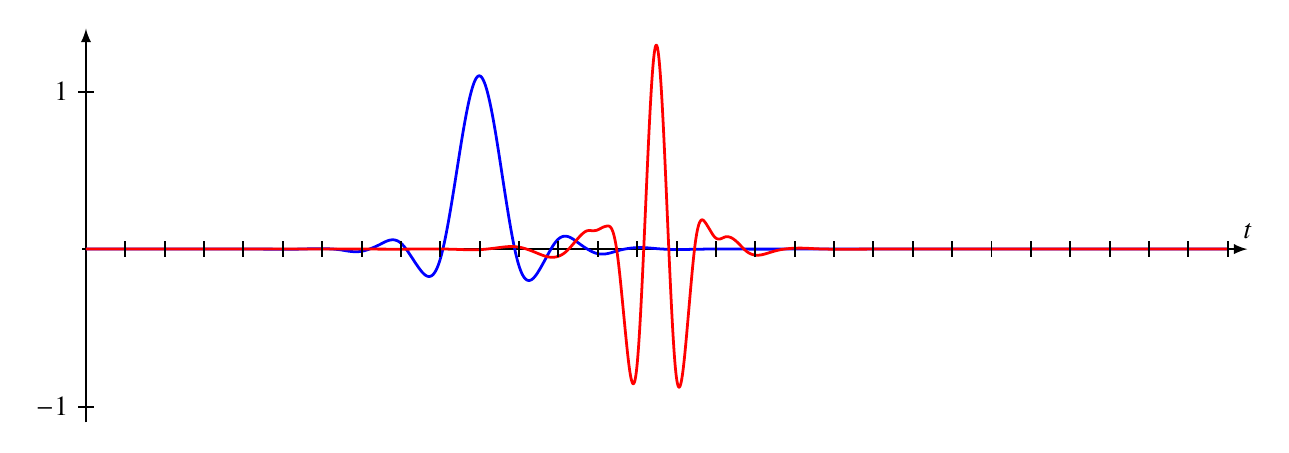
\begin{tikzpicture}[>=latex,yscale=2,xscale=0.5]

\draw[->,line width=0.7pt] (-0.1,0)--(29.5,0) coordinate[label={$t$}];
\draw[->,line width=0.7pt] (0,-1.1)--(0,1.4);

\draw[line width=1pt,color=blue] (0.00000, -0.00000)
(0.00195, 0.00000)
--(0.00391, 0.00000)
--(0.00586, -0.00000)
--(0.00781, -0.00000)
--(0.00977, 0.00000)
--(0.01172, 0.00000)
--(0.01367, -0.00000)
--(0.01562, 0.00000)
--(0.01758, 0.00000)
--(0.01953, 0.00000)
--(0.02148, 0.00000)
--(0.02344, -0.00000)
--(0.02539, -0.00000)
--(0.02734, -0.00000)
--(0.02930, -0.00000)
--(0.03125, 0.00000)
--(0.03320, 0.00000)
--(0.03516, 0.00000)
--(0.03711, -0.00000)
--(0.03906, -0.00000)
--(0.04102, -0.00000)
--(0.04297, -0.00000)
--(0.04492, 0.00000)
--(0.04688, 0.00000)
--(0.04883, 0.00000)
--(0.05078, -0.00000)
--(0.05273, -0.00000)
--(0.05469, -0.00000)
--(0.05664, -0.00000)
--(0.05859, -0.00000)
--(0.06055, -0.00000)
--(0.06250, -0.00000)
--(0.06445, -0.00000)
--(0.06641, 0.00000)
--(0.06836, 0.00000)
--(0.07031, 0.00000)
--(0.07227, 0.00000)
--(0.07422, 0.00000)
--(0.07617, 0.00000)
--(0.07812, 0.00000)
--(0.08008, -0.00000)
--(0.08203, -0.00000)
--(0.08398, -0.00000)
--(0.08594, -0.00000)
--(0.08789, -0.00000)
--(0.08984, -0.00000)
--(0.09180, -0.00000)
--(0.09375, 0.00000)
--(0.09570, 0.00000)
--(0.09766, 0.00000)
--(0.09961, 0.00000)
--(0.10156, 0.00000)
--(0.10352, 0.00000)
--(0.10547, 0.00000)
--(0.10742, -0.00000)
--(0.10938, -0.00000)
--(0.11133, -0.00000)
--(0.11328, -0.00000)
--(0.11523, -0.00000)
--(0.11719, -0.00000)
--(0.11914, 0.00000)
--(0.12109, 0.00000)
--(0.12305, 0.00000)
--(0.12500, 0.00000)
--(0.12695, 0.00000)
--(0.12891, 0.00000)
--(0.13086, 0.00000)
--(0.13281, 0.00000)
--(0.13477, 0.00000)
--(0.13672, 0.00000)
--(0.13867, 0.00000)
--(0.14062, 0.00000)
--(0.14258, 0.00000)
--(0.14453, 0.00000)
--(0.14648, 0.00000)
--(0.14844, 0.00000)
--(0.15039, 0.00000)
--(0.15234, -0.00000)
--(0.15430, -0.00000)
--(0.15625, -0.00000)
--(0.15820, -0.00000)
--(0.16016, -0.00000)
--(0.16211, -0.00000)
--(0.16406, -0.00000)
--(0.16602, -0.00000)
--(0.16797, -0.00000)
--(0.16992, -0.00000)
--(0.17188, -0.00000)
--(0.17383, -0.00000)
--(0.17578, -0.00000)
--(0.17773, -0.00000)
--(0.17969, 0.00000)
--(0.18164, 0.00000)
--(0.18359, 0.00000)
--(0.18555, 0.00000)
--(0.18750, 0.00000)
--(0.18945, 0.00000)
--(0.19141, 0.00000)
--(0.19336, 0.00000)
--(0.19531, 0.00000)
--(0.19727, 0.00000)
--(0.19922, 0.00000)
--(0.20117, 0.00000)
--(0.20312, 0.00000)
--(0.20508, 0.00000)
--(0.20703, -0.00000)
--(0.20898, -0.00000)
--(0.21094, -0.00000)
--(0.21289, -0.00000)
--(0.21484, -0.00000)
--(0.21680, -0.00000)
--(0.21875, -0.00000)
--(0.22070, -0.00000)
--(0.22266, -0.00000)
--(0.22461, -0.00000)
--(0.22656, -0.00000)
--(0.22852, -0.00000)
--(0.23047, -0.00000)
--(0.23242, -0.00000)
--(0.23438, 0.00000)
--(0.23633, 0.00000)
--(0.23828, 0.00000)
--(0.24023, 0.00000)
--(0.24219, 0.00000)
--(0.24414, 0.00000)
--(0.24609, 0.00000)
--(0.24805, 0.00000)
--(0.25000, 0.00000)
--(0.25195, 0.00000)
--(0.25391, 0.00000)
--(0.25586, 0.00000)
--(0.25781, -0.00000)
--(0.25977, -0.00000)
--(0.26172, -0.00000)
--(0.26367, -0.00000)
--(0.26562, -0.00000)
--(0.26758, -0.00000)
--(0.26953, -0.00000)
--(0.27148, -0.00000)
--(0.27344, -0.00000)
--(0.27539, -0.00000)
--(0.27734, -0.00000)
--(0.27930, -0.00000)
--(0.28125, -0.00000)
--(0.28320, -0.00000)
--(0.28516, -0.00000)
--(0.28711, -0.00000)
--(0.28906, -0.00000)
--(0.29102, -0.00000)
--(0.29297, -0.00000)
--(0.29492, -0.00000)
--(0.29688, -0.00000)
--(0.29883, -0.00000)
--(0.30078, -0.00000)
--(0.30273, -0.00000)
--(0.30469, -0.00000)
--(0.30664, -0.00000)
--(0.30859, -0.00000)
--(0.31055, -0.00000)
--(0.31250, -0.00000)
--(0.31445, -0.00000)
--(0.31641, -0.00000)
--(0.31836, -0.00000)
--(0.32031, -0.00000)
--(0.32227, 0.00000)
--(0.32422, 0.00000)
--(0.32617, 0.00000)
--(0.32812, 0.00000)
--(0.33008, 0.00000)
--(0.33203, 0.00000)
--(0.33398, 0.00000)
--(0.33594, 0.00000)
--(0.33789, 0.00000)
--(0.33984, 0.00000)
--(0.34180, 0.00000)
--(0.34375, 0.00000)
--(0.34570, 0.00000)
--(0.34766, 0.00000)
--(0.34961, 0.00000)
--(0.35156, 0.00000)
--(0.35352, 0.00000)
--(0.35547, 0.00000)
--(0.35742, 0.00000)
--(0.35938, 0.00000)
--(0.36133, 0.00000)
--(0.36328, 0.00000)
--(0.36523, 0.00000)
--(0.36719, 0.00000)
--(0.36914, 0.00000)
--(0.37109, 0.00000)
--(0.37305, 0.00000)
--(0.37500, 0.00000)
--(0.37695, -0.00000)
--(0.37891, -0.00000)
--(0.38086, -0.00000)
--(0.38281, -0.00000)
--(0.38477, -0.00000)
--(0.38672, -0.00000)
--(0.38867, -0.00000)
--(0.39062, -0.00000)
--(0.39258, -0.00000)
--(0.39453, -0.00000)
--(0.39648, -0.00000)
--(0.39844, -0.00000)
--(0.40039, -0.00000)
--(0.40234, -0.00000)
--(0.40430, -0.00000)
--(0.40625, -0.00000)
--(0.40820, -0.00000)
--(0.41016, -0.00000)
--(0.41211, -0.00000)
--(0.41406, -0.00000)
--(0.41602, -0.00000)
--(0.41797, -0.00000)
--(0.41992, -0.00000)
--(0.42188, -0.00000)
--(0.42383, -0.00000)
--(0.42578, -0.00000)
--(0.42773, -0.00000)
--(0.42969, -0.00000)
--(0.43164, 0.00000)
--(0.43359, 0.00000)
--(0.43555, 0.00000)
--(0.43750, 0.00000)
--(0.43945, 0.00000)
--(0.44141, 0.00000)
--(0.44336, 0.00000)
--(0.44531, 0.00000)
--(0.44727, 0.00000)
--(0.44922, 0.00000)
--(0.45117, 0.00000)
--(0.45312, 0.00000)
--(0.45508, 0.00000)
--(0.45703, 0.00000)
--(0.45898, 0.00000)
--(0.46094, 0.00000)
--(0.46289, 0.00000)
--(0.46484, 0.00000)
--(0.46680, 0.00000)
--(0.46875, 0.00000)
--(0.47070, 0.00000)
--(0.47266, 0.00000)
--(0.47461, 0.00000)
--(0.47656, 0.00000)
--(0.47852, 0.00000)
--(0.48047, 0.00000)
--(0.48242, 0.00000)
--(0.48438, 0.00000)
--(0.48633, -0.00000)
--(0.48828, -0.00000)
--(0.49023, -0.00000)
--(0.49219, -0.00000)
--(0.49414, -0.00000)
--(0.49609, -0.00000)
--(0.49805, -0.00000)
--(0.50000, -0.00000)
--(0.50195, -0.00000)
--(0.50391, -0.00000)
--(0.50586, -0.00000)
--(0.50781, -0.00000)
--(0.50977, -0.00000)
--(0.51172, -0.00000)
--(0.51367, -0.00000)
--(0.51562, -0.00000)
--(0.51758, -0.00000)
--(0.51953, -0.00000)
--(0.52148, -0.00000)
--(0.52344, -0.00000)
--(0.52539, -0.00000)
--(0.52734, -0.00000)
--(0.52930, -0.00000)
--(0.53125, -0.00000)
--(0.53320, -0.00000)
--(0.53516, 0.00000)
--(0.53711, 0.00000)
--(0.53906, 0.00000)
--(0.54102, 0.00000)
--(0.54297, 0.00000)
--(0.54492, 0.00000)
--(0.54688, 0.00000)
--(0.54883, 0.00000)
--(0.55078, 0.00000)
--(0.55273, 0.00000)
--(0.55469, 0.00000)
--(0.55664, 0.00000)
--(0.55859, 0.00000)
--(0.56055, 0.00000)
--(0.56250, 0.00000)
--(0.56445, 0.00000)
--(0.56641, 0.00000)
--(0.56836, 0.00000)
--(0.57031, 0.00000)
--(0.57227, 0.00000)
--(0.57422, 0.00000)
--(0.57617, 0.00000)
--(0.57812, 0.00000)
--(0.58008, 0.00000)
--(0.58203, 0.00000)
--(0.58398, 0.00000)
--(0.58594, 0.00000)
--(0.58789, 0.00000)
--(0.58984, 0.00000)
--(0.59180, 0.00000)
--(0.59375, 0.00000)
--(0.59570, 0.00000)
--(0.59766, 0.00000)
--(0.59961, 0.00000)
--(0.60156, 0.00000)
--(0.60352, 0.00000)
--(0.60547, 0.00000)
--(0.60742, 0.00000)
--(0.60938, 0.00000)
--(0.61133, 0.00000)
--(0.61328, 0.00000)
--(0.61523, 0.00000)
--(0.61719, 0.00000)
--(0.61914, 0.00000)
--(0.62109, 0.00000)
--(0.62305, 0.00000)
--(0.62500, 0.00000)
--(0.62695, 0.00000)
--(0.62891, 0.00000)
--(0.63086, 0.00000)
--(0.63281, 0.00000)
--(0.63477, 0.00000)
--(0.63672, 0.00000)
--(0.63867, 0.00000)
--(0.64062, 0.00000)
--(0.64258, 0.00000)
--(0.64453, 0.00000)
--(0.64648, 0.00000)
--(0.64844, 0.00000)
--(0.65039, 0.00000)
--(0.65234, 0.00000)
--(0.65430, 0.00000)
--(0.65625, 0.00000)
--(0.65820, 0.00000)
--(0.66016, 0.00000)
--(0.66211, -0.00000)
--(0.66406, -0.00000)
--(0.66602, -0.00000)
--(0.66797, -0.00000)
--(0.66992, -0.00000)
--(0.67188, -0.00000)
--(0.67383, -0.00000)
--(0.67578, -0.00000)
--(0.67773, -0.00000)
--(0.67969, -0.00000)
--(0.68164, -0.00000)
--(0.68359, -0.00000)
--(0.68555, -0.00000)
--(0.68750, -0.00000)
--(0.68945, -0.00000)
--(0.69141, -0.00000)
--(0.69336, -0.00000)
--(0.69531, -0.00000)
--(0.69727, -0.00000)
--(0.69922, -0.00000)
--(0.70117, -0.00000)
--(0.70312, -0.00000)
--(0.70508, -0.00000)
--(0.70703, -0.00000)
--(0.70898, -0.00000)
--(0.71094, -0.00000)
--(0.71289, -0.00000)
--(0.71484, -0.00000)
--(0.71680, -0.00000)
--(0.71875, -0.00000)
--(0.72070, -0.00000)
--(0.72266, -0.00000)
--(0.72461, -0.00000)
--(0.72656, -0.00000)
--(0.72852, -0.00000)
--(0.73047, -0.00000)
--(0.73242, -0.00000)
--(0.73438, -0.00000)
--(0.73633, -0.00000)
--(0.73828, -0.00000)
--(0.74023, -0.00000)
--(0.74219, -0.00000)
--(0.74414, -0.00000)
--(0.74609, -0.00000)
--(0.74805, -0.00000)
--(0.75000, -0.00000)
--(0.75195, -0.00000)
--(0.75391, -0.00000)
--(0.75586, -0.00000)
--(0.75781, -0.00000)
--(0.75977, -0.00000)
--(0.76172, -0.00000)
--(0.76367, -0.00000)
--(0.76562, -0.00000)
--(0.76758, -0.00000)
--(0.76953, -0.00000)
--(0.77148, 0.00000)
--(0.77344, 0.00000)
--(0.77539, 0.00000)
--(0.77734, 0.00000)
--(0.77930, 0.00000)
--(0.78125, 0.00000)
--(0.78320, 0.00000)
--(0.78516, 0.00000)
--(0.78711, 0.00000)
--(0.78906, 0.00000)
--(0.79102, 0.00000)
--(0.79297, 0.00000)
--(0.79492, 0.00000)
--(0.79688, 0.00000)
--(0.79883, 0.00000)
--(0.80078, 0.00000)
--(0.80273, 0.00000)
--(0.80469, 0.00000)
--(0.80664, 0.00000)
--(0.80859, 0.00000)
--(0.81055, 0.00000)
--(0.81250, 0.00000)
--(0.81445, 0.00000)
--(0.81641, 0.00000)
--(0.81836, 0.00000)
--(0.82031, 0.00000)
--(0.82227, 0.00000)
--(0.82422, 0.00000)
--(0.82617, 0.00000)
--(0.82812, 0.00000)
--(0.83008, 0.00000)
--(0.83203, 0.00000)
--(0.83398, 0.00000)
--(0.83594, 0.00000)
--(0.83789, 0.00000)
--(0.83984, 0.00000)
--(0.84180, 0.00000)
--(0.84375, 0.00000)
--(0.84570, 0.00000)
--(0.84766, 0.00000)
--(0.84961, 0.00000)
--(0.85156, 0.00000)
--(0.85352, 0.00000)
--(0.85547, 0.00000)
--(0.85742, 0.00000)
--(0.85938, 0.00000)
--(0.86133, 0.00000)
--(0.86328, 0.00000)
--(0.86523, 0.00000)
--(0.86719, 0.00000)
--(0.86914, 0.00000)
--(0.87109, 0.00000)
--(0.87305, 0.00000)
--(0.87500, 0.00000)
--(0.87695, 0.00000)
--(0.87891, 0.00000)
--(0.88086, -0.00000)
--(0.88281, -0.00000)
--(0.88477, -0.00000)
--(0.88672, -0.00000)
--(0.88867, -0.00000)
--(0.89062, -0.00000)
--(0.89258, -0.00000)
--(0.89453, -0.00000)
--(0.89648, -0.00000)
--(0.89844, -0.00000)
--(0.90039, -0.00000)
--(0.90234, -0.00000)
--(0.90430, -0.00000)
--(0.90625, -0.00000)
--(0.90820, -0.00000)
--(0.91016, -0.00000)
--(0.91211, -0.00000)
--(0.91406, -0.00000)
--(0.91602, -0.00000)
--(0.91797, -0.00000)
--(0.91992, -0.00000)
--(0.92188, -0.00000)
--(0.92383, -0.00000)
--(0.92578, -0.00000)
--(0.92773, -0.00000)
--(0.92969, -0.00000)
--(0.93164, -0.00000)
--(0.93359, -0.00000)
--(0.93555, -0.00000)
--(0.93750, -0.00000)
--(0.93945, -0.00000)
--(0.94141, -0.00000)
--(0.94336, -0.00000)
--(0.94531, -0.00000)
--(0.94727, -0.00000)
--(0.94922, -0.00000)
--(0.95117, -0.00000)
--(0.95312, -0.00000)
--(0.95508, -0.00000)
--(0.95703, -0.00000)
--(0.95898, -0.00000)
--(0.96094, -0.00000)
--(0.96289, -0.00000)
--(0.96484, -0.00000)
--(0.96680, -0.00000)
--(0.96875, -0.00000)
--(0.97070, -0.00000)
--(0.97266, -0.00000)
--(0.97461, -0.00000)
--(0.97656, -0.00000)
--(0.97852, -0.00000)
--(0.98047, -0.00000)
--(0.98242, -0.00000)
--(0.98438, -0.00000)
--(0.98633, -0.00000)
--(0.98828, -0.00000)
--(0.99023, -0.00000)
--(0.99219, 0.00000)
--(0.99414, 0.00000)
--(0.99609, 0.00000)
--(0.99805, 0.00000)
--(1.00000, 0.00000)
--(1.00195, 0.00000)
--(1.00391, 0.00000)
--(1.00586, 0.00000)
--(1.00781, 0.00000)
--(1.00977, 0.00000)
--(1.01172, 0.00000)
--(1.01367, 0.00000)
--(1.01562, 0.00000)
--(1.01758, 0.00000)
--(1.01953, 0.00000)
--(1.02148, 0.00000)
--(1.02344, 0.00000)
--(1.02539, 0.00000)
--(1.02734, 0.00000)
--(1.02930, 0.00000)
--(1.03125, 0.00000)
--(1.03320, 0.00000)
--(1.03516, 0.00000)
--(1.03711, 0.00000)
--(1.03906, 0.00000)
--(1.04102, 0.00000)
--(1.04297, 0.00000)
--(1.04492, 0.00000)
--(1.04688, 0.00000)
--(1.04883, 0.00000)
--(1.05078, 0.00000)
--(1.05273, 0.00000)
--(1.05469, 0.00000)
--(1.05664, 0.00000)
--(1.05859, 0.00000)
--(1.06055, 0.00000)
--(1.06250, 0.00000)
--(1.06445, 0.00000)
--(1.06641, 0.00000)
--(1.06836, 0.00000)
--(1.07031, 0.00000)
--(1.07227, 0.00000)
--(1.07422, 0.00000)
--(1.07617, 0.00000)
--(1.07812, 0.00000)
--(1.08008, 0.00000)
--(1.08203, 0.00000)
--(1.08398, 0.00000)
--(1.08594, 0.00000)
--(1.08789, -0.00000)
--(1.08984, -0.00000)
--(1.09180, -0.00000)
--(1.09375, -0.00000)
--(1.09570, -0.00000)
--(1.09766, -0.00000)
--(1.09961, -0.00000)
--(1.10156, -0.00000)
--(1.10352, -0.00000)
--(1.10547, -0.00000)
--(1.10742, -0.00000)
--(1.10938, -0.00000)
--(1.11133, -0.00000)
--(1.11328, -0.00000)
--(1.11523, -0.00000)
--(1.11719, -0.00000)
--(1.11914, -0.00000)
--(1.12109, -0.00000)
--(1.12305, -0.00000)
--(1.12500, -0.00000)
--(1.12695, -0.00000)
--(1.12891, -0.00000)
--(1.13086, -0.00000)
--(1.13281, -0.00000)
--(1.13477, -0.00000)
--(1.13672, -0.00000)
--(1.13867, -0.00000)
--(1.14062, -0.00000)
--(1.14258, -0.00000)
--(1.14453, -0.00000)
--(1.14648, -0.00000)
--(1.14844, -0.00000)
--(1.15039, -0.00000)
--(1.15234, -0.00000)
--(1.15430, -0.00000)
--(1.15625, -0.00000)
--(1.15820, -0.00000)
--(1.16016, -0.00000)
--(1.16211, -0.00000)
--(1.16406, -0.00000)
--(1.16602, -0.00000)
--(1.16797, -0.00000)
--(1.16992, -0.00000)
--(1.17188, -0.00000)
--(1.17383, -0.00000)
--(1.17578, -0.00000)
--(1.17773, -0.00000)
--(1.17969, -0.00000)
--(1.18164, -0.00000)
--(1.18359, -0.00000)
--(1.18555, -0.00000)
--(1.18750, -0.00000)
--(1.18945, -0.00000)
--(1.19141, -0.00000)
--(1.19336, -0.00000)
--(1.19531, -0.00000)
--(1.19727, -0.00000)
--(1.19922, -0.00000)
--(1.20117, -0.00000)
--(1.20312, -0.00000)
--(1.20508, -0.00000)
--(1.20703, -0.00000)
--(1.20898, -0.00000)
--(1.21094, -0.00000)
--(1.21289, -0.00000)
--(1.21484, -0.00000)
--(1.21680, -0.00000)
--(1.21875, -0.00000)
--(1.22070, -0.00000)
--(1.22266, -0.00000)
--(1.22461, -0.00000)
--(1.22656, -0.00000)
--(1.22852, -0.00000)
--(1.23047, -0.00000)
--(1.23242, -0.00000)
--(1.23438, -0.00000)
--(1.23633, -0.00000)
--(1.23828, -0.00000)
--(1.24023, -0.00000)
--(1.24219, -0.00000)
--(1.24414, -0.00000)
--(1.24609, -0.00000)
--(1.24805, -0.00000)
--(1.25000, -0.00000)
--(1.25195, -0.00000)
--(1.25391, -0.00000)
--(1.25586, -0.00000)
--(1.25781, -0.00000)
--(1.25977, -0.00000)
--(1.26172, -0.00000)
--(1.26367, -0.00000)
--(1.26562, -0.00000)
--(1.26758, -0.00000)
--(1.26953, -0.00000)
--(1.27148, -0.00000)
--(1.27344, -0.00000)
--(1.27539, -0.00000)
--(1.27734, -0.00000)
--(1.27930, -0.00000)
--(1.28125, -0.00000)
--(1.28320, -0.00000)
--(1.28516, -0.00000)
--(1.28711, -0.00000)
--(1.28906, -0.00000)
--(1.29102, -0.00000)
--(1.29297, -0.00000)
--(1.29492, -0.00000)
--(1.29688, -0.00000)
--(1.29883, -0.00000)
--(1.30078, -0.00000)
--(1.30273, -0.00000)
--(1.30469, -0.00000)
--(1.30664, -0.00000)
--(1.30859, -0.00000)
--(1.31055, -0.00000)
--(1.31250, -0.00000)
--(1.31445, -0.00000)
--(1.31641, -0.00000)
--(1.31836, -0.00000)
--(1.32031, -0.00000)
--(1.32227, -0.00000)
--(1.32422, -0.00000)
--(1.32617, -0.00000)
--(1.32812, -0.00000)
--(1.33008, -0.00000)
--(1.33203, -0.00000)
--(1.33398, -0.00000)
--(1.33594, -0.00000)
--(1.33789, -0.00000)
--(1.33984, -0.00000)
--(1.34180, 0.00000)
--(1.34375, 0.00000)
--(1.34570, 0.00000)
--(1.34766, 0.00000)
--(1.34961, 0.00000)
--(1.35156, 0.00000)
--(1.35352, 0.00000)
--(1.35547, 0.00000)
--(1.35742, 0.00000)
--(1.35938, 0.00000)
--(1.36133, 0.00000)
--(1.36328, 0.00000)
--(1.36523, 0.00000)
--(1.36719, 0.00000)
--(1.36914, 0.00000)
--(1.37109, 0.00000)
--(1.37305, 0.00000)
--(1.37500, 0.00000)
--(1.37695, 0.00000)
--(1.37891, 0.00000)
--(1.38086, 0.00000)
--(1.38281, 0.00000)
--(1.38477, 0.00000)
--(1.38672, 0.00000)
--(1.38867, 0.00000)
--(1.39062, 0.00000)
--(1.39258, 0.00000)
--(1.39453, 0.00000)
--(1.39648, 0.00000)
--(1.39844, 0.00000)
--(1.40039, 0.00000)
--(1.40234, 0.00000)
--(1.40430, 0.00000)
--(1.40625, 0.00000)
--(1.40820, 0.00000)
--(1.41016, 0.00000)
--(1.41211, 0.00000)
--(1.41406, 0.00000)
--(1.41602, 0.00000)
--(1.41797, 0.00000)
--(1.41992, 0.00000)
--(1.42188, 0.00000)
--(1.42383, 0.00000)
--(1.42578, 0.00000)
--(1.42773, 0.00000)
--(1.42969, 0.00000)
--(1.43164, 0.00000)
--(1.43359, 0.00000)
--(1.43555, 0.00000)
--(1.43750, 0.00000)
--(1.43945, 0.00000)
--(1.44141, 0.00000)
--(1.44336, 0.00000)
--(1.44531, 0.00000)
--(1.44727, 0.00000)
--(1.44922, 0.00000)
--(1.45117, 0.00000)
--(1.45312, 0.00000)
--(1.45508, 0.00000)
--(1.45703, 0.00000)
--(1.45898, 0.00000)
--(1.46094, 0.00000)
--(1.46289, 0.00000)
--(1.46484, 0.00000)
--(1.46680, 0.00000)
--(1.46875, 0.00000)
--(1.47070, 0.00000)
--(1.47266, 0.00000)
--(1.47461, 0.00000)
--(1.47656, 0.00000)
--(1.47852, 0.00000)
--(1.48047, 0.00000)
--(1.48242, 0.00000)
--(1.48438, 0.00000)
--(1.48633, 0.00000)
--(1.48828, 0.00000)
--(1.49023, 0.00000)
--(1.49219, 0.00000)
--(1.49414, 0.00000)
--(1.49609, 0.00000)
--(1.49805, 0.00000)
--(1.50000, 0.00000)
--(1.50195, 0.00000)
--(1.50391, 0.00000)
--(1.50586, 0.00000)
--(1.50781, 0.00000)
--(1.50977, 0.00000)
--(1.51172, 0.00000)
--(1.51367, 0.00000)
--(1.51562, 0.00000)
--(1.51758, 0.00000)
--(1.51953, 0.00000)
--(1.52148, 0.00000)
--(1.52344, 0.00000)
--(1.52539, 0.00000)
--(1.52734, 0.00000)
--(1.52930, 0.00000)
--(1.53125, 0.00000)
--(1.53320, 0.00000)
--(1.53516, 0.00000)
--(1.53711, 0.00000)
--(1.53906, 0.00000)
--(1.54102, 0.00000)
--(1.54297, 0.00000)
--(1.54492, 0.00000)
--(1.54688, 0.00000)
--(1.54883, 0.00000)
--(1.55078, 0.00000)
--(1.55273, 0.00000)
--(1.55469, 0.00000)
--(1.55664, 0.00000)
--(1.55859, 0.00000)
--(1.56055, -0.00000)
--(1.56250, -0.00000)
--(1.56445, -0.00000)
--(1.56641, -0.00000)
--(1.56836, -0.00000)
--(1.57031, -0.00000)
--(1.57227, -0.00000)
--(1.57422, -0.00000)
--(1.57617, -0.00000)
--(1.57812, -0.00000)
--(1.58008, -0.00000)
--(1.58203, -0.00000)
--(1.58398, -0.00000)
--(1.58594, -0.00000)
--(1.58789, -0.00000)
--(1.58984, -0.00000)
--(1.59180, -0.00000)
--(1.59375, -0.00000)
--(1.59570, -0.00000)
--(1.59766, -0.00000)
--(1.59961, -0.00000)
--(1.60156, -0.00000)
--(1.60352, -0.00000)
--(1.60547, -0.00000)
--(1.60742, -0.00000)
--(1.60938, -0.00000)
--(1.61133, -0.00000)
--(1.61328, -0.00000)
--(1.61523, -0.00000)
--(1.61719, -0.00000)
--(1.61914, -0.00000)
--(1.62109, -0.00000)
--(1.62305, -0.00000)
--(1.62500, -0.00000)
--(1.62695, -0.00000)
--(1.62891, -0.00000)
--(1.63086, -0.00000)
--(1.63281, -0.00000)
--(1.63477, -0.00000)
--(1.63672, -0.00000)
--(1.63867, -0.00000)
--(1.64062, -0.00000)
--(1.64258, -0.00000)
--(1.64453, -0.00000)
--(1.64648, -0.00000)
--(1.64844, -0.00000)
--(1.65039, -0.00000)
--(1.65234, -0.00000)
--(1.65430, -0.00000)
--(1.65625, -0.00000)
--(1.65820, -0.00000)
--(1.66016, -0.00000)
--(1.66211, -0.00000)
--(1.66406, -0.00000)
--(1.66602, -0.00000)
--(1.66797, -0.00000)
--(1.66992, -0.00000)
--(1.67188, -0.00000)
--(1.67383, -0.00000)
--(1.67578, -0.00000)
--(1.67773, -0.00000)
--(1.67969, -0.00000)
--(1.68164, -0.00000)
--(1.68359, -0.00000)
--(1.68555, -0.00000)
--(1.68750, -0.00000)
--(1.68945, -0.00000)
--(1.69141, -0.00000)
--(1.69336, -0.00000)
--(1.69531, -0.00000)
--(1.69727, -0.00000)
--(1.69922, -0.00000)
--(1.70117, -0.00000)
--(1.70312, -0.00000)
--(1.70508, -0.00000)
--(1.70703, -0.00000)
--(1.70898, -0.00000)
--(1.71094, -0.00000)
--(1.71289, -0.00000)
--(1.71484, -0.00000)
--(1.71680, -0.00000)
--(1.71875, -0.00000)
--(1.72070, -0.00000)
--(1.72266, -0.00000)
--(1.72461, -0.00000)
--(1.72656, -0.00000)
--(1.72852, -0.00000)
--(1.73047, -0.00000)
--(1.73242, -0.00000)
--(1.73438, -0.00000)
--(1.73633, -0.00000)
--(1.73828, -0.00000)
--(1.74023, -0.00000)
--(1.74219, -0.00000)
--(1.74414, -0.00000)
--(1.74609, -0.00000)
--(1.74805, -0.00000)
--(1.75000, -0.00000)
--(1.75195, -0.00000)
--(1.75391, -0.00000)
--(1.75586, -0.00000)
--(1.75781, -0.00000)
--(1.75977, -0.00000)
--(1.76172, -0.00000)
--(1.76367, -0.00000)
--(1.76562, -0.00000)
--(1.76758, -0.00000)
--(1.76953, -0.00000)
--(1.77148, -0.00000)
--(1.77344, -0.00000)
--(1.77539, -0.00000)
--(1.77734, -0.00000)
--(1.77930, 0.00000)
--(1.78125, 0.00000)
--(1.78320, 0.00000)
--(1.78516, 0.00000)
--(1.78711, 0.00000)
--(1.78906, 0.00000)
--(1.79102, 0.00000)
--(1.79297, 0.00000)
--(1.79492, 0.00000)
--(1.79688, 0.00000)
--(1.79883, 0.00000)
--(1.80078, 0.00000)
--(1.80273, 0.00000)
--(1.80469, 0.00000)
--(1.80664, 0.00000)
--(1.80859, 0.00000)
--(1.81055, 0.00000)
--(1.81250, 0.00000)
--(1.81445, 0.00000)
--(1.81641, 0.00000)
--(1.81836, 0.00000)
--(1.82031, 0.00000)
--(1.82227, 0.00000)
--(1.82422, 0.00000)
--(1.82617, 0.00000)
--(1.82812, 0.00000)
--(1.83008, 0.00000)
--(1.83203, 0.00000)
--(1.83398, 0.00000)
--(1.83594, 0.00000)
--(1.83789, 0.00000)
--(1.83984, 0.00000)
--(1.84180, 0.00000)
--(1.84375, 0.00000)
--(1.84570, 0.00000)
--(1.84766, 0.00000)
--(1.84961, 0.00000)
--(1.85156, 0.00000)
--(1.85352, 0.00000)
--(1.85547, 0.00000)
--(1.85742, 0.00000)
--(1.85938, 0.00000)
--(1.86133, 0.00000)
--(1.86328, 0.00000)
--(1.86523, 0.00000)
--(1.86719, 0.00000)
--(1.86914, 0.00000)
--(1.87109, 0.00000)
--(1.87305, 0.00000)
--(1.87500, 0.00000)
--(1.87695, 0.00000)
--(1.87891, 0.00000)
--(1.88086, 0.00000)
--(1.88281, 0.00000)
--(1.88477, 0.00000)
--(1.88672, 0.00000)
--(1.88867, 0.00000)
--(1.89062, 0.00000)
--(1.89258, 0.00000)
--(1.89453, 0.00000)
--(1.89648, 0.00000)
--(1.89844, 0.00000)
--(1.90039, 0.00000)
--(1.90234, 0.00000)
--(1.90430, 0.00000)
--(1.90625, 0.00000)
--(1.90820, 0.00000)
--(1.91016, 0.00000)
--(1.91211, 0.00000)
--(1.91406, 0.00000)
--(1.91602, 0.00000)
--(1.91797, 0.00000)
--(1.91992, 0.00000)
--(1.92188, 0.00000)
--(1.92383, 0.00000)
--(1.92578, 0.00000)
--(1.92773, 0.00000)
--(1.92969, 0.00000)
--(1.93164, 0.00000)
--(1.93359, 0.00000)
--(1.93555, 0.00000)
--(1.93750, 0.00000)
--(1.93945, 0.00000)
--(1.94141, 0.00000)
--(1.94336, 0.00000)
--(1.94531, 0.00000)
--(1.94727, 0.00000)
--(1.94922, 0.00000)
--(1.95117, 0.00000)
--(1.95312, 0.00000)
--(1.95508, 0.00000)
--(1.95703, 0.00000)
--(1.95898, 0.00000)
--(1.96094, 0.00000)
--(1.96289, 0.00000)
--(1.96484, 0.00000)
--(1.96680, 0.00000)
--(1.96875, 0.00000)
--(1.97070, 0.00000)
--(1.97266, 0.00000)
--(1.97461, 0.00000)
--(1.97656, 0.00000)
--(1.97852, 0.00000)
--(1.98047, 0.00000)
--(1.98242, 0.00000)
--(1.98438, 0.00000)
--(1.98633, 0.00000)
--(1.98828, 0.00000)
--(1.99023, 0.00000)
--(1.99219, 0.00000)
--(1.99414, 0.00000)
--(1.99609, 0.00000)
--(1.99805, 0.00000)
--(2.00000, 0.00000)
--(2.00195, 0.00000)
--(2.00391, -0.00000)
--(2.00586, -0.00000)
--(2.00781, -0.00000)
--(2.00977, -0.00000)
--(2.01172, -0.00000)
--(2.01367, -0.00000)
--(2.01562, -0.00000)
--(2.01758, -0.00000)
--(2.01953, -0.00000)
--(2.02148, -0.00000)
--(2.02344, -0.00000)
--(2.02539, -0.00000)
--(2.02734, -0.00000)
--(2.02930, -0.00000)
--(2.03125, -0.00000)
--(2.03320, -0.00000)
--(2.03516, -0.00000)
--(2.03711, -0.00000)
--(2.03906, -0.00000)
--(2.04102, -0.00000)
--(2.04297, -0.00000)
--(2.04492, -0.00000)
--(2.04688, -0.00000)
--(2.04883, -0.00000)
--(2.05078, -0.00000)
--(2.05273, -0.00000)
--(2.05469, -0.00000)
--(2.05664, -0.00000)
--(2.05859, -0.00000)
--(2.06055, -0.00000)
--(2.06250, -0.00000)
--(2.06445, -0.00000)
--(2.06641, -0.00000)
--(2.06836, -0.00000)
--(2.07031, -0.00000)
--(2.07227, -0.00000)
--(2.07422, -0.00000)
--(2.07617, -0.00000)
--(2.07812, -0.00000)
--(2.08008, -0.00000)
--(2.08203, -0.00000)
--(2.08398, -0.00000)
--(2.08594, -0.00000)
--(2.08789, -0.00000)
--(2.08984, -0.00000)
--(2.09180, -0.00000)
--(2.09375, -0.00000)
--(2.09570, -0.00000)
--(2.09766, -0.00000)
--(2.09961, -0.00000)
--(2.10156, -0.00000)
--(2.10352, -0.00000)
--(2.10547, -0.00000)
--(2.10742, -0.00000)
--(2.10938, -0.00000)
--(2.11133, -0.00000)
--(2.11328, -0.00000)
--(2.11523, -0.00000)
--(2.11719, -0.00000)
--(2.11914, -0.00000)
--(2.12109, -0.00000)
--(2.12305, -0.00000)
--(2.12500, -0.00000)
--(2.12695, -0.00000)
--(2.12891, -0.00000)
--(2.13086, -0.00000)
--(2.13281, -0.00000)
--(2.13477, -0.00000)
--(2.13672, -0.00000)
--(2.13867, -0.00000)
--(2.14062, -0.00000)
--(2.14258, -0.00000)
--(2.14453, -0.00000)
--(2.14648, -0.00000)
--(2.14844, -0.00000)
--(2.15039, -0.00000)
--(2.15234, -0.00000)
--(2.15430, -0.00000)
--(2.15625, -0.00000)
--(2.15820, -0.00000)
--(2.16016, -0.00000)
--(2.16211, -0.00000)
--(2.16406, -0.00000)
--(2.16602, -0.00000)
--(2.16797, -0.00000)
--(2.16992, -0.00000)
--(2.17188, -0.00000)
--(2.17383, -0.00000)
--(2.17578, -0.00000)
--(2.17773, -0.00000)
--(2.17969, -0.00000)
--(2.18164, -0.00000)
--(2.18359, -0.00000)
--(2.18555, -0.00000)
--(2.18750, -0.00000)
--(2.18945, -0.00000)
--(2.19141, -0.00000)
--(2.19336, 0.00000)
--(2.19531, 0.00000)
--(2.19727, 0.00000)
--(2.19922, 0.00000)
--(2.20117, 0.00000)
--(2.20312, 0.00000)
--(2.20508, 0.00000)
--(2.20703, 0.00000)
--(2.20898, 0.00000)
--(2.21094, 0.00000)
--(2.21289, 0.00000)
--(2.21484, 0.00000)
--(2.21680, 0.00000)
--(2.21875, 0.00000)
--(2.22070, 0.00000)
--(2.22266, 0.00000)
--(2.22461, 0.00000)
--(2.22656, 0.00000)
--(2.22852, 0.00000)
--(2.23047, 0.00000)
--(2.23242, 0.00000)
--(2.23438, 0.00000)
--(2.23633, 0.00000)
--(2.23828, 0.00000)
--(2.24023, 0.00000)
--(2.24219, 0.00000)
--(2.24414, 0.00000)
--(2.24609, 0.00000)
--(2.24805, 0.00000)
--(2.25000, 0.00000)
--(2.25195, 0.00000)
--(2.25391, 0.00000)
--(2.25586, 0.00000)
--(2.25781, 0.00000)
--(2.25977, 0.00000)
--(2.26172, 0.00000)
--(2.26367, 0.00000)
--(2.26562, 0.00000)
--(2.26758, 0.00000)
--(2.26953, 0.00000)
--(2.27148, 0.00000)
--(2.27344, 0.00000)
--(2.27539, 0.00000)
--(2.27734, 0.00000)
--(2.27930, 0.00000)
--(2.28125, 0.00000)
--(2.28320, 0.00000)
--(2.28516, 0.00000)
--(2.28711, 0.00000)
--(2.28906, 0.00000)
--(2.29102, 0.00000)
--(2.29297, 0.00000)
--(2.29492, 0.00000)
--(2.29688, 0.00000)
--(2.29883, 0.00000)
--(2.30078, 0.00000)
--(2.30273, 0.00000)
--(2.30469, 0.00000)
--(2.30664, 0.00000)
--(2.30859, 0.00000)
--(2.31055, 0.00000)
--(2.31250, 0.00000)
--(2.31445, 0.00000)
--(2.31641, 0.00000)
--(2.31836, 0.00000)
--(2.32031, 0.00000)
--(2.32227, 0.00000)
--(2.32422, 0.00000)
--(2.32617, 0.00000)
--(2.32812, 0.00000)
--(2.33008, 0.00000)
--(2.33203, 0.00000)
--(2.33398, 0.00000)
--(2.33594, 0.00000)
--(2.33789, 0.00000)
--(2.33984, 0.00000)
--(2.34180, 0.00000)
--(2.34375, 0.00000)
--(2.34570, 0.00000)
--(2.34766, 0.00000)
--(2.34961, 0.00000)
--(2.35156, 0.00000)
--(2.35352, 0.00000)
--(2.35547, 0.00000)
--(2.35742, 0.00000)
--(2.35938, 0.00000)
--(2.36133, 0.00000)
--(2.36328, 0.00000)
--(2.36523, 0.00000)
--(2.36719, 0.00000)
--(2.36914, 0.00000)
--(2.37109, 0.00000)
--(2.37305, 0.00000)
--(2.37500, 0.00000)
--(2.37695, 0.00000)
--(2.37891, 0.00000)
--(2.38086, 0.00000)
--(2.38281, 0.00000)
--(2.38477, 0.00000)
--(2.38672, 0.00000)
--(2.38867, 0.00000)
--(2.39062, 0.00000)
--(2.39258, 0.00000)
--(2.39453, 0.00000)
--(2.39648, 0.00000)
--(2.39844, 0.00000)
--(2.40039, 0.00000)
--(2.40234, 0.00000)
--(2.40430, 0.00000)
--(2.40625, 0.00000)
--(2.40820, 0.00000)
--(2.41016, 0.00000)
--(2.41211, 0.00000)
--(2.41406, 0.00000)
--(2.41602, 0.00000)
--(2.41797, 0.00000)
--(2.41992, 0.00000)
--(2.42188, 0.00000)
--(2.42383, 0.00000)
--(2.42578, 0.00000)
--(2.42773, 0.00000)
--(2.42969, 0.00000)
--(2.43164, 0.00000)
--(2.43359, 0.00000)
--(2.43555, 0.00000)
--(2.43750, 0.00000)
--(2.43945, 0.00000)
--(2.44141, 0.00000)
--(2.44336, 0.00000)
--(2.44531, 0.00000)
--(2.44727, 0.00000)
--(2.44922, 0.00000)
--(2.45117, 0.00000)
--(2.45312, 0.00000)
--(2.45508, 0.00000)
--(2.45703, 0.00000)
--(2.45898, 0.00000)
--(2.46094, 0.00000)
--(2.46289, 0.00000)
--(2.46484, 0.00000)
--(2.46680, 0.00000)
--(2.46875, 0.00000)
--(2.47070, 0.00000)
--(2.47266, 0.00000)
--(2.47461, 0.00000)
--(2.47656, 0.00000)
--(2.47852, 0.00000)
--(2.48047, 0.00000)
--(2.48242, 0.00000)
--(2.48438, 0.00000)
--(2.48633, 0.00000)
--(2.48828, 0.00000)
--(2.49023, 0.00000)
--(2.49219, 0.00000)
--(2.49414, 0.00000)
--(2.49609, 0.00000)
--(2.49805, 0.00000)
--(2.50000, 0.00000)
--(2.50195, 0.00000)
--(2.50391, 0.00000)
--(2.50586, 0.00000)
--(2.50781, 0.00000)
--(2.50977, 0.00000)
--(2.51172, 0.00000)
--(2.51367, 0.00000)
--(2.51562, 0.00000)
--(2.51758, 0.00000)
--(2.51953, 0.00000)
--(2.52148, 0.00000)
--(2.52344, 0.00000)
--(2.52539, 0.00000)
--(2.52734, 0.00000)
--(2.52930, 0.00000)
--(2.53125, 0.00000)
--(2.53320, 0.00000)
--(2.53516, 0.00000)
--(2.53711, 0.00000)
--(2.53906, 0.00000)
--(2.54102, 0.00000)
--(2.54297, 0.00000)
--(2.54492, 0.00000)
--(2.54688, 0.00000)
--(2.54883, 0.00000)
--(2.55078, 0.00000)
--(2.55273, 0.00000)
--(2.55469, 0.00000)
--(2.55664, 0.00000)
--(2.55859, 0.00000)
--(2.56055, 0.00000)
--(2.56250, 0.00000)
--(2.56445, 0.00000)
--(2.56641, 0.00000)
--(2.56836, 0.00000)
--(2.57031, 0.00000)
--(2.57227, 0.00000)
--(2.57422, 0.00000)
--(2.57617, 0.00000)
--(2.57812, 0.00000)
--(2.58008, 0.00000)
--(2.58203, 0.00000)
--(2.58398, 0.00000)
--(2.58594, 0.00000)
--(2.58789, 0.00000)
--(2.58984, 0.00000)
--(2.59180, 0.00000)
--(2.59375, 0.00000)
--(2.59570, 0.00000)
--(2.59766, 0.00000)
--(2.59961, 0.00000)
--(2.60156, 0.00000)
--(2.60352, 0.00000)
--(2.60547, 0.00000)
--(2.60742, 0.00000)
--(2.60938, 0.00000)
--(2.61133, 0.00000)
--(2.61328, 0.00000)
--(2.61523, 0.00000)
--(2.61719, 0.00000)
--(2.61914, 0.00000)
--(2.62109, 0.00000)
--(2.62305, 0.00000)
--(2.62500, 0.00000)
--(2.62695, 0.00000)
--(2.62891, 0.00000)
--(2.63086, 0.00000)
--(2.63281, 0.00000)
--(2.63477, 0.00000)
--(2.63672, 0.00000)
--(2.63867, 0.00000)
--(2.64062, 0.00000)
--(2.64258, 0.00000)
--(2.64453, 0.00000)
--(2.64648, 0.00000)
--(2.64844, 0.00000)
--(2.65039, 0.00000)
--(2.65234, 0.00000)
--(2.65430, 0.00000)
--(2.65625, 0.00000)
--(2.65820, 0.00000)
--(2.66016, 0.00000)
--(2.66211, 0.00000)
--(2.66406, 0.00000)
--(2.66602, 0.00000)
--(2.66797, 0.00000)
--(2.66992, 0.00000)
--(2.67188, 0.00000)
--(2.67383, 0.00000)
--(2.67578, 0.00000)
--(2.67773, 0.00000)
--(2.67969, 0.00000)
--(2.68164, 0.00000)
--(2.68359, 0.00000)
--(2.68555, 0.00000)
--(2.68750, 0.00000)
--(2.68945, 0.00000)
--(2.69141, 0.00000)
--(2.69336, 0.00000)
--(2.69531, 0.00000)
--(2.69727, 0.00000)
--(2.69922, 0.00000)
--(2.70117, -0.00000)
--(2.70312, -0.00000)
--(2.70508, -0.00000)
--(2.70703, -0.00000)
--(2.70898, -0.00000)
--(2.71094, -0.00000)
--(2.71289, -0.00000)
--(2.71484, -0.00000)
--(2.71680, -0.00000)
--(2.71875, -0.00000)
--(2.72070, -0.00000)
--(2.72266, -0.00000)
--(2.72461, -0.00000)
--(2.72656, -0.00000)
--(2.72852, -0.00000)
--(2.73047, -0.00000)
--(2.73242, -0.00000)
--(2.73438, -0.00000)
--(2.73633, -0.00000)
--(2.73828, -0.00000)
--(2.74023, -0.00000)
--(2.74219, -0.00000)
--(2.74414, -0.00000)
--(2.74609, -0.00000)
--(2.74805, -0.00000)
--(2.75000, -0.00000)
--(2.75195, -0.00000)
--(2.75391, -0.00000)
--(2.75586, -0.00000)
--(2.75781, -0.00000)
--(2.75977, -0.00000)
--(2.76172, -0.00000)
--(2.76367, -0.00000)
--(2.76562, -0.00000)
--(2.76758, -0.00000)
--(2.76953, -0.00000)
--(2.77148, -0.00000)
--(2.77344, -0.00000)
--(2.77539, -0.00000)
--(2.77734, -0.00000)
--(2.77930, -0.00000)
--(2.78125, -0.00000)
--(2.78320, -0.00000)
--(2.78516, -0.00000)
--(2.78711, -0.00000)
--(2.78906, -0.00000)
--(2.79102, -0.00000)
--(2.79297, -0.00000)
--(2.79492, -0.00000)
--(2.79688, -0.00000)
--(2.79883, -0.00000)
--(2.80078, -0.00000)
--(2.80273, -0.00000)
--(2.80469, -0.00000)
--(2.80664, -0.00000)
--(2.80859, -0.00000)
--(2.81055, -0.00000)
--(2.81250, -0.00000)
--(2.81445, -0.00000)
--(2.81641, -0.00000)
--(2.81836, -0.00000)
--(2.82031, -0.00000)
--(2.82227, -0.00000)
--(2.82422, -0.00000)
--(2.82617, -0.00000)
--(2.82812, -0.00000)
--(2.83008, -0.00000)
--(2.83203, -0.00000)
--(2.83398, -0.00000)
--(2.83594, -0.00000)
--(2.83789, -0.00000)
--(2.83984, -0.00000)
--(2.84180, -0.00000)
--(2.84375, -0.00000)
--(2.84570, -0.00000)
--(2.84766, -0.00000)
--(2.84961, -0.00000)
--(2.85156, -0.00000)
--(2.85352, -0.00000)
--(2.85547, -0.00000)
--(2.85742, -0.00000)
--(2.85938, -0.00000)
--(2.86133, -0.00000)
--(2.86328, -0.00000)
--(2.86523, -0.00000)
--(2.86719, -0.00000)
--(2.86914, -0.00000)
--(2.87109, -0.00000)
--(2.87305, -0.00000)
--(2.87500, -0.00000)
--(2.87695, -0.00000)
--(2.87891, -0.00000)
--(2.88086, -0.00000)
--(2.88281, -0.00000)
--(2.88477, -0.00000)
--(2.88672, -0.00000)
--(2.88867, -0.00000)
--(2.89062, -0.00000)
--(2.89258, -0.00000)
--(2.89453, -0.00000)
--(2.89648, -0.00000)
--(2.89844, -0.00000)
--(2.90039, -0.00000)
--(2.90234, -0.00000)
--(2.90430, -0.00000)
--(2.90625, -0.00000)
--(2.90820, -0.00000)
--(2.91016, -0.00000)
--(2.91211, -0.00000)
--(2.91406, -0.00000)
--(2.91602, -0.00000)
--(2.91797, -0.00000)
--(2.91992, -0.00000)
--(2.92188, -0.00000)
--(2.92383, -0.00000)
--(2.92578, -0.00000)
--(2.92773, -0.00000)
--(2.92969, -0.00000)
--(2.93164, -0.00000)
--(2.93359, -0.00000)
--(2.93555, -0.00000)
--(2.93750, -0.00000)
--(2.93945, -0.00000)
--(2.94141, -0.00000)
--(2.94336, -0.00000)
--(2.94531, -0.00000)
--(2.94727, -0.00000)
--(2.94922, -0.00000)
--(2.95117, -0.00000)
--(2.95312, -0.00000)
--(2.95508, -0.00000)
--(2.95703, -0.00000)
--(2.95898, -0.00000)
--(2.96094, -0.00000)
--(2.96289, -0.00000)
--(2.96484, -0.00000)
--(2.96680, -0.00000)
--(2.96875, -0.00000)
--(2.97070, -0.00000)
--(2.97266, -0.00000)
--(2.97461, -0.00000)
--(2.97656, -0.00000)
--(2.97852, -0.00000)
--(2.98047, -0.00000)
--(2.98242, -0.00000)
--(2.98438, -0.00000)
--(2.98633, -0.00000)
--(2.98828, -0.00000)
--(2.99023, -0.00000)
--(2.99219, -0.00000)
--(2.99414, -0.00000)
--(2.99609, -0.00000)
--(2.99805, -0.00000)
--(3.00000, -0.00000)
--(3.00195, -0.00000)
--(3.00391, -0.00000)
--(3.00586, -0.00000)
--(3.00781, -0.00000)
--(3.00977, -0.00000)
--(3.01172, -0.00000)
--(3.01367, -0.00000)
--(3.01562, -0.00000)
--(3.01758, -0.00000)
--(3.01953, -0.00000)
--(3.02148, -0.00000)
--(3.02344, -0.00000)
--(3.02539, -0.00000)
--(3.02734, -0.00000)
--(3.02930, -0.00000)
--(3.03125, -0.00000)
--(3.03320, -0.00000)
--(3.03516, -0.00000)
--(3.03711, -0.00000)
--(3.03906, -0.00000)
--(3.04102, -0.00000)
--(3.04297, -0.00000)
--(3.04492, -0.00000)
--(3.04688, -0.00000)
--(3.04883, -0.00000)
--(3.05078, -0.00000)
--(3.05273, -0.00000)
--(3.05469, -0.00000)
--(3.05664, -0.00000)
--(3.05859, -0.00000)
--(3.06055, -0.00000)
--(3.06250, -0.00000)
--(3.06445, -0.00000)
--(3.06641, -0.00000)
--(3.06836, -0.00000)
--(3.07031, -0.00000)
--(3.07227, -0.00000)
--(3.07422, -0.00000)
--(3.07617, -0.00000)
--(3.07812, -0.00000)
--(3.08008, -0.00000)
--(3.08203, -0.00000)
--(3.08398, -0.00000)
--(3.08594, -0.00000)
--(3.08789, -0.00000)
--(3.08984, -0.00000)
--(3.09180, -0.00000)
--(3.09375, -0.00000)
--(3.09570, -0.00000)
--(3.09766, -0.00000)
--(3.09961, -0.00000)
--(3.10156, -0.00000)
--(3.10352, -0.00000)
--(3.10547, -0.00000)
--(3.10742, -0.00000)
--(3.10938, -0.00000)
--(3.11133, -0.00000)
--(3.11328, -0.00000)
--(3.11523, -0.00000)
--(3.11719, -0.00000)
--(3.11914, -0.00000)
--(3.12109, -0.00000)
--(3.12305, -0.00000)
--(3.12500, -0.00000)
--(3.12695, -0.00000)
--(3.12891, -0.00000)
--(3.13086, -0.00000)
--(3.13281, -0.00000)
--(3.13477, -0.00000)
--(3.13672, -0.00000)
--(3.13867, -0.00000)
--(3.14062, -0.00000)
--(3.14258, 0.00000)
--(3.14453, 0.00000)
--(3.14648, 0.00000)
--(3.14844, 0.00000)
--(3.15039, 0.00000)
--(3.15234, 0.00000)
--(3.15430, 0.00000)
--(3.15625, 0.00000)
--(3.15820, 0.00000)
--(3.16016, 0.00000)
--(3.16211, 0.00000)
--(3.16406, 0.00000)
--(3.16602, 0.00000)
--(3.16797, 0.00000)
--(3.16992, 0.00000)
--(3.17188, 0.00000)
--(3.17383, 0.00000)
--(3.17578, 0.00000)
--(3.17773, 0.00000)
--(3.17969, 0.00000)
--(3.18164, 0.00000)
--(3.18359, 0.00000)
--(3.18555, 0.00000)
--(3.18750, 0.00000)
--(3.18945, 0.00000)
--(3.19141, 0.00000)
--(3.19336, 0.00000)
--(3.19531, 0.00000)
--(3.19727, 0.00000)
--(3.19922, 0.00000)
--(3.20117, 0.00000)
--(3.20312, 0.00000)
--(3.20508, 0.00000)
--(3.20703, 0.00000)
--(3.20898, 0.00000)
--(3.21094, 0.00000)
--(3.21289, 0.00000)
--(3.21484, 0.00000)
--(3.21680, 0.00000)
--(3.21875, 0.00000)
--(3.22070, 0.00000)
--(3.22266, 0.00000)
--(3.22461, 0.00000)
--(3.22656, 0.00000)
--(3.22852, 0.00000)
--(3.23047, 0.00000)
--(3.23242, 0.00000)
--(3.23438, 0.00000)
--(3.23633, 0.00000)
--(3.23828, 0.00000)
--(3.24023, 0.00000)
--(3.24219, 0.00000)
--(3.24414, 0.00000)
--(3.24609, 0.00000)
--(3.24805, 0.00000)
--(3.25000, 0.00000)
--(3.25195, 0.00000)
--(3.25391, 0.00000)
--(3.25586, 0.00000)
--(3.25781, 0.00000)
--(3.25977, 0.00000)
--(3.26172, 0.00000)
--(3.26367, 0.00000)
--(3.26562, 0.00000)
--(3.26758, 0.00000)
--(3.26953, 0.00000)
--(3.27148, 0.00000)
--(3.27344, 0.00000)
--(3.27539, 0.00000)
--(3.27734, 0.00000)
--(3.27930, 0.00000)
--(3.28125, 0.00000)
--(3.28320, 0.00000)
--(3.28516, 0.00000)
--(3.28711, 0.00000)
--(3.28906, 0.00000)
--(3.29102, 0.00000)
--(3.29297, 0.00000)
--(3.29492, 0.00000)
--(3.29688, 0.00000)
--(3.29883, 0.00000)
--(3.30078, 0.00000)
--(3.30273, 0.00000)
--(3.30469, 0.00000)
--(3.30664, 0.00000)
--(3.30859, 0.00000)
--(3.31055, 0.00000)
--(3.31250, 0.00000)
--(3.31445, 0.00000)
--(3.31641, 0.00000)
--(3.31836, 0.00000)
--(3.32031, 0.00000)
--(3.32227, 0.00000)
--(3.32422, 0.00000)
--(3.32617, 0.00000)
--(3.32812, 0.00000)
--(3.33008, 0.00000)
--(3.33203, 0.00000)
--(3.33398, 0.00000)
--(3.33594, 0.00000)
--(3.33789, 0.00000)
--(3.33984, 0.00000)
--(3.34180, 0.00001)
--(3.34375, 0.00001)
--(3.34570, 0.00001)
--(3.34766, 0.00001)
--(3.34961, 0.00001)
--(3.35156, 0.00001)
--(3.35352, 0.00001)
--(3.35547, 0.00001)
--(3.35742, 0.00001)
--(3.35938, 0.00001)
--(3.36133, 0.00001)
--(3.36328, 0.00001)
--(3.36523, 0.00001)
--(3.36719, 0.00001)
--(3.36914, 0.00001)
--(3.37109, 0.00001)
--(3.37305, 0.00001)
--(3.37500, 0.00001)
--(3.37695, 0.00001)
--(3.37891, 0.00001)
--(3.38086, 0.00001)
--(3.38281, 0.00001)
--(3.38477, 0.00001)
--(3.38672, 0.00001)
--(3.38867, 0.00001)
--(3.39062, 0.00001)
--(3.39258, 0.00001)
--(3.39453, 0.00001)
--(3.39648, 0.00001)
--(3.39844, 0.00001)
--(3.40039, 0.00001)
--(3.40234, 0.00001)
--(3.40430, 0.00001)
--(3.40625, 0.00001)
--(3.40820, 0.00001)
--(3.41016, 0.00001)
--(3.41211, 0.00001)
--(3.41406, 0.00001)
--(3.41602, 0.00001)
--(3.41797, 0.00001)
--(3.41992, 0.00001)
--(3.42188, 0.00001)
--(3.42383, 0.00001)
--(3.42578, 0.00001)
--(3.42773, 0.00001)
--(3.42969, 0.00001)
--(3.43164, 0.00001)
--(3.43359, 0.00001)
--(3.43555, 0.00001)
--(3.43750, 0.00001)
--(3.43945, 0.00001)
--(3.44141, 0.00001)
--(3.44336, 0.00001)
--(3.44531, 0.00001)
--(3.44727, 0.00001)
--(3.44922, 0.00001)
--(3.45117, 0.00001)
--(3.45312, 0.00001)
--(3.45508, 0.00001)
--(3.45703, 0.00001)
--(3.45898, 0.00001)
--(3.46094, 0.00001)
--(3.46289, 0.00001)
--(3.46484, 0.00001)
--(3.46680, 0.00001)
--(3.46875, 0.00001)
--(3.47070, 0.00001)
--(3.47266, 0.00001)
--(3.47461, 0.00001)
--(3.47656, 0.00001)
--(3.47852, 0.00001)
--(3.48047, 0.00001)
--(3.48242, 0.00001)
--(3.48438, 0.00001)
--(3.48633, 0.00001)
--(3.48828, 0.00000)
--(3.49023, 0.00000)
--(3.49219, 0.00000)
--(3.49414, 0.00000)
--(3.49609, 0.00000)
--(3.49805, 0.00000)
--(3.50000, 0.00000)
--(3.50195, 0.00000)
--(3.50391, 0.00000)
--(3.50586, 0.00000)
--(3.50781, 0.00000)
--(3.50977, 0.00000)
--(3.51172, 0.00000)
--(3.51367, 0.00000)
--(3.51562, 0.00000)
--(3.51758, 0.00000)
--(3.51953, 0.00000)
--(3.52148, 0.00000)
--(3.52344, 0.00000)
--(3.52539, 0.00000)
--(3.52734, 0.00000)
--(3.52930, 0.00000)
--(3.53125, 0.00000)
--(3.53320, 0.00000)
--(3.53516, 0.00000)
--(3.53711, 0.00000)
--(3.53906, 0.00000)
--(3.54102, 0.00000)
--(3.54297, 0.00000)
--(3.54492, 0.00000)
--(3.54688, 0.00000)
--(3.54883, 0.00000)
--(3.55078, 0.00000)
--(3.55273, 0.00000)
--(3.55469, 0.00000)
--(3.55664, 0.00000)
--(3.55859, 0.00000)
--(3.56055, 0.00000)
--(3.56250, 0.00000)
--(3.56445, 0.00000)
--(3.56641, 0.00000)
--(3.56836, 0.00000)
--(3.57031, 0.00000)
--(3.57227, 0.00000)
--(3.57422, 0.00000)
--(3.57617, 0.00000)
--(3.57812, 0.00000)
--(3.58008, -0.00000)
--(3.58203, -0.00000)
--(3.58398, -0.00000)
--(3.58594, -0.00000)
--(3.58789, -0.00000)
--(3.58984, -0.00000)
--(3.59180, -0.00000)
--(3.59375, -0.00000)
--(3.59570, -0.00000)
--(3.59766, -0.00000)
--(3.59961, -0.00000)
--(3.60156, -0.00000)
--(3.60352, -0.00000)
--(3.60547, -0.00000)
--(3.60742, -0.00000)
--(3.60938, -0.00000)
--(3.61133, -0.00000)
--(3.61328, -0.00000)
--(3.61523, -0.00000)
--(3.61719, -0.00000)
--(3.61914, -0.00000)
--(3.62109, -0.00000)
--(3.62305, -0.00000)
--(3.62500, -0.00000)
--(3.62695, -0.00000)
--(3.62891, -0.00000)
--(3.63086, -0.00000)
--(3.63281, -0.00000)
--(3.63477, -0.00000)
--(3.63672, -0.00000)
--(3.63867, -0.00000)
--(3.64062, -0.00000)
--(3.64258, -0.00000)
--(3.64453, -0.00000)
--(3.64648, -0.00000)
--(3.64844, -0.00000)
--(3.65039, -0.00001)
--(3.65234, -0.00001)
--(3.65430, -0.00001)
--(3.65625, -0.00001)
--(3.65820, -0.00001)
--(3.66016, -0.00001)
--(3.66211, -0.00001)
--(3.66406, -0.00001)
--(3.66602, -0.00001)
--(3.66797, -0.00001)
--(3.66992, -0.00001)
--(3.67188, -0.00001)
--(3.67383, -0.00001)
--(3.67578, -0.00001)
--(3.67773, -0.00001)
--(3.67969, -0.00001)
--(3.68164, -0.00001)
--(3.68359, -0.00001)
--(3.68555, -0.00001)
--(3.68750, -0.00001)
--(3.68945, -0.00001)
--(3.69141, -0.00001)
--(3.69336, -0.00001)
--(3.69531, -0.00001)
--(3.69727, -0.00001)
--(3.69922, -0.00001)
--(3.70117, -0.00001)
--(3.70312, -0.00001)
--(3.70508, -0.00001)
--(3.70703, -0.00001)
--(3.70898, -0.00001)
--(3.71094, -0.00001)
--(3.71289, -0.00001)
--(3.71484, -0.00001)
--(3.71680, -0.00001)
--(3.71875, -0.00001)
--(3.72070, -0.00001)
--(3.72266, -0.00001)
--(3.72461, -0.00001)
--(3.72656, -0.00001)
--(3.72852, -0.00001)
--(3.73047, -0.00001)
--(3.73242, -0.00001)
--(3.73438, -0.00001)
--(3.73633, -0.00001)
--(3.73828, -0.00001)
--(3.74023, -0.00001)
--(3.74219, -0.00001)
--(3.74414, -0.00001)
--(3.74609, -0.00001)
--(3.74805, -0.00001)
--(3.75000, -0.00001)
--(3.75195, -0.00001)
--(3.75391, -0.00001)
--(3.75586, -0.00001)
--(3.75781, -0.00001)
--(3.75977, -0.00001)
--(3.76172, -0.00001)
--(3.76367, -0.00001)
--(3.76562, -0.00001)
--(3.76758, -0.00001)
--(3.76953, -0.00001)
--(3.77148, -0.00001)
--(3.77344, -0.00001)
--(3.77539, -0.00001)
--(3.77734, -0.00001)
--(3.77930, -0.00001)
--(3.78125, -0.00001)
--(3.78320, -0.00001)
--(3.78516, -0.00001)
--(3.78711, -0.00001)
--(3.78906, -0.00001)
--(3.79102, -0.00001)
--(3.79297, -0.00001)
--(3.79492, -0.00001)
--(3.79688, -0.00001)
--(3.79883, -0.00001)
--(3.80078, -0.00002)
--(3.80273, -0.00002)
--(3.80469, -0.00002)
--(3.80664, -0.00002)
--(3.80859, -0.00002)
--(3.81055, -0.00002)
--(3.81250, -0.00002)
--(3.81445, -0.00002)
--(3.81641, -0.00002)
--(3.81836, -0.00002)
--(3.82031, -0.00002)
--(3.82227, -0.00002)
--(3.82422, -0.00002)
--(3.82617, -0.00002)
--(3.82812, -0.00002)
--(3.83008, -0.00002)
--(3.83203, -0.00002)
--(3.83398, -0.00002)
--(3.83594, -0.00002)
--(3.83789, -0.00002)
--(3.83984, -0.00002)
--(3.84180, -0.00002)
--(3.84375, -0.00002)
--(3.84570, -0.00002)
--(3.84766, -0.00002)
--(3.84961, -0.00002)
--(3.85156, -0.00002)
--(3.85352, -0.00002)
--(3.85547, -0.00002)
--(3.85742, -0.00002)
--(3.85938, -0.00002)
--(3.86133, -0.00002)
--(3.86328, -0.00002)
--(3.86523, -0.00002)
--(3.86719, -0.00002)
--(3.86914, -0.00002)
--(3.87109, -0.00002)
--(3.87305, -0.00002)
--(3.87500, -0.00002)
--(3.87695, -0.00002)
--(3.87891, -0.00002)
--(3.88086, -0.00002)
--(3.88281, -0.00002)
--(3.88477, -0.00002)
--(3.88672, -0.00002)
--(3.88867, -0.00002)
--(3.89062, -0.00002)
--(3.89258, -0.00002)
--(3.89453, -0.00002)
--(3.89648, -0.00002)
--(3.89844, -0.00002)
--(3.90039, -0.00002)
--(3.90234, -0.00002)
--(3.90430, -0.00002)
--(3.90625, -0.00002)
--(3.90820, -0.00002)
--(3.91016, -0.00002)
--(3.91211, -0.00002)
--(3.91406, -0.00002)
--(3.91602, -0.00002)
--(3.91797, -0.00002)
--(3.91992, -0.00002)
--(3.92188, -0.00002)
--(3.92383, -0.00002)
--(3.92578, -0.00002)
--(3.92773, -0.00002)
--(3.92969, -0.00002)
--(3.93164, -0.00001)
--(3.93359, -0.00001)
--(3.93555, -0.00001)
--(3.93750, -0.00001)
--(3.93945, -0.00001)
--(3.94141, -0.00001)
--(3.94336, -0.00001)
--(3.94531, -0.00001)
--(3.94727, -0.00001)
--(3.94922, -0.00001)
--(3.95117, -0.00001)
--(3.95312, -0.00001)
--(3.95508, -0.00001)
--(3.95703, -0.00001)
--(3.95898, -0.00001)
--(3.96094, -0.00001)
--(3.96289, -0.00001)
--(3.96484, -0.00001)
--(3.96680, -0.00001)
--(3.96875, -0.00001)
--(3.97070, -0.00001)
--(3.97266, -0.00001)
--(3.97461, -0.00001)
--(3.97656, -0.00001)
--(3.97852, -0.00001)
--(3.98047, -0.00001)
--(3.98242, -0.00001)
--(3.98438, -0.00001)
--(3.98633, -0.00001)
--(3.98828, -0.00001)
--(3.99023, -0.00001)
--(3.99219, -0.00001)
--(3.99414, -0.00001)
--(3.99609, -0.00001)
--(3.99805, -0.00001)
--(4.00000, -0.00001)
--(4.00195, -0.00001)
--(4.00391, -0.00001)
--(4.00586, -0.00001)
--(4.00781, -0.00001)
--(4.00977, -0.00000)
--(4.01172, -0.00000)
--(4.01367, -0.00000)
--(4.01562, -0.00000)
--(4.01758, -0.00000)
--(4.01953, -0.00000)
--(4.02148, -0.00000)
--(4.02344, -0.00000)
--(4.02539, -0.00000)
--(4.02734, -0.00000)
--(4.02930, -0.00000)
--(4.03125, -0.00000)
--(4.03320, 0.00000)
--(4.03516, 0.00000)
--(4.03711, 0.00000)
--(4.03906, 0.00000)
--(4.04102, 0.00000)
--(4.04297, 0.00000)
--(4.04492, 0.00000)
--(4.04688, 0.00000)
--(4.04883, 0.00000)
--(4.05078, 0.00000)
--(4.05273, 0.00000)
--(4.05469, 0.00001)
--(4.05664, 0.00001)
--(4.05859, 0.00001)
--(4.06055, 0.00001)
--(4.06250, 0.00001)
--(4.06445, 0.00001)
--(4.06641, 0.00001)
--(4.06836, 0.00001)
--(4.07031, 0.00001)
--(4.07227, 0.00001)
--(4.07422, 0.00001)
--(4.07617, 0.00001)
--(4.07812, 0.00001)
--(4.08008, 0.00001)
--(4.08203, 0.00001)
--(4.08398, 0.00001)
--(4.08594, 0.00001)
--(4.08789, 0.00001)
--(4.08984, 0.00001)
--(4.09180, 0.00001)
--(4.09375, 0.00001)
--(4.09570, 0.00001)
--(4.09766, 0.00002)
--(4.09961, 0.00002)
--(4.10156, 0.00002)
--(4.10352, 0.00002)
--(4.10547, 0.00002)
--(4.10742, 0.00002)
--(4.10938, 0.00002)
--(4.11133, 0.00002)
--(4.11328, 0.00002)
--(4.11523, 0.00002)
--(4.11719, 0.00002)
--(4.11914, 0.00002)
--(4.12109, 0.00002)
--(4.12305, 0.00002)
--(4.12500, 0.00002)
--(4.12695, 0.00002)
--(4.12891, 0.00002)
--(4.13086, 0.00002)
--(4.13281, 0.00002)
--(4.13477, 0.00002)
--(4.13672, 0.00002)
--(4.13867, 0.00002)
--(4.14062, 0.00002)
--(4.14258, 0.00003)
--(4.14453, 0.00003)
--(4.14648, 0.00003)
--(4.14844, 0.00003)
--(4.15039, 0.00003)
--(4.15234, 0.00003)
--(4.15430, 0.00003)
--(4.15625, 0.00003)
--(4.15820, 0.00003)
--(4.16016, 0.00003)
--(4.16211, 0.00003)
--(4.16406, 0.00003)
--(4.16602, 0.00003)
--(4.16797, 0.00003)
--(4.16992, 0.00003)
--(4.17188, 0.00003)
--(4.17383, 0.00003)
--(4.17578, 0.00003)
--(4.17773, 0.00003)
--(4.17969, 0.00003)
--(4.18164, 0.00003)
--(4.18359, 0.00003)
--(4.18555, 0.00003)
--(4.18750, 0.00003)
--(4.18945, 0.00003)
--(4.19141, 0.00003)
--(4.19336, 0.00003)
--(4.19531, 0.00003)
--(4.19727, 0.00003)
--(4.19922, 0.00003)
--(4.20117, 0.00003)
--(4.20312, 0.00003)
--(4.20508, 0.00003)
--(4.20703, 0.00003)
--(4.20898, 0.00004)
--(4.21094, 0.00004)
--(4.21289, 0.00004)
--(4.21484, 0.00004)
--(4.21680, 0.00004)
--(4.21875, 0.00004)
--(4.22070, 0.00004)
--(4.22266, 0.00004)
--(4.22461, 0.00004)
--(4.22656, 0.00004)
--(4.22852, 0.00004)
--(4.23047, 0.00004)
--(4.23242, 0.00004)
--(4.23438, 0.00004)
--(4.23633, 0.00004)
--(4.23828, 0.00004)
--(4.24023, 0.00004)
--(4.24219, 0.00004)
--(4.24414, 0.00004)
--(4.24609, 0.00004)
--(4.24805, 0.00004)
--(4.25000, 0.00004)
--(4.25195, 0.00004)
--(4.25391, 0.00004)
--(4.25586, 0.00004)
--(4.25781, 0.00004)
--(4.25977, 0.00004)
--(4.26172, 0.00004)
--(4.26367, 0.00004)
--(4.26562, 0.00004)
--(4.26758, 0.00004)
--(4.26953, 0.00004)
--(4.27148, 0.00004)
--(4.27344, 0.00004)
--(4.27539, 0.00004)
--(4.27734, 0.00004)
--(4.27930, 0.00004)
--(4.28125, 0.00003)
--(4.28320, 0.00003)
--(4.28516, 0.00003)
--(4.28711, 0.00003)
--(4.28906, 0.00003)
--(4.29102, 0.00003)
--(4.29297, 0.00003)
--(4.29492, 0.00003)
--(4.29688, 0.00003)
--(4.29883, 0.00003)
--(4.30078, 0.00003)
--(4.30273, 0.00003)
--(4.30469, 0.00003)
--(4.30664, 0.00003)
--(4.30859, 0.00003)
--(4.31055, 0.00003)
--(4.31250, 0.00003)
--(4.31445, 0.00003)
--(4.31641, 0.00003)
--(4.31836, 0.00003)
--(4.32031, 0.00003)
--(4.32227, 0.00003)
--(4.32422, 0.00003)
--(4.32617, 0.00003)
--(4.32812, 0.00003)
--(4.33008, 0.00003)
--(4.33203, 0.00003)
--(4.33398, 0.00003)
--(4.33594, 0.00003)
--(4.33789, 0.00003)
--(4.33984, 0.00003)
--(4.34180, 0.00003)
--(4.34375, 0.00003)
--(4.34570, 0.00002)
--(4.34766, 0.00002)
--(4.34961, 0.00002)
--(4.35156, 0.00002)
--(4.35352, 0.00002)
--(4.35547, 0.00002)
--(4.35742, 0.00002)
--(4.35938, 0.00002)
--(4.36133, 0.00002)
--(4.36328, 0.00002)
--(4.36523, 0.00002)
--(4.36719, 0.00002)
--(4.36914, 0.00002)
--(4.37109, 0.00002)
--(4.37305, 0.00002)
--(4.37500, 0.00002)
--(4.37695, 0.00002)
--(4.37891, 0.00002)
--(4.38086, 0.00002)
--(4.38281, 0.00002)
--(4.38477, 0.00002)
--(4.38672, 0.00002)
--(4.38867, 0.00002)
--(4.39062, 0.00001)
--(4.39258, 0.00001)
--(4.39453, 0.00001)
--(4.39648, 0.00001)
--(4.39844, 0.00001)
--(4.40039, 0.00001)
--(4.40234, 0.00001)
--(4.40430, 0.00001)
--(4.40625, 0.00001)
--(4.40820, 0.00001)
--(4.41016, 0.00001)
--(4.41211, 0.00001)
--(4.41406, 0.00001)
--(4.41602, 0.00001)
--(4.41797, 0.00001)
--(4.41992, 0.00001)
--(4.42188, 0.00001)
--(4.42383, 0.00001)
--(4.42578, 0.00000)
--(4.42773, 0.00000)
--(4.42969, 0.00000)
--(4.43164, 0.00000)
--(4.43359, 0.00000)
--(4.43555, 0.00000)
--(4.43750, 0.00000)
--(4.43945, 0.00000)
--(4.44141, -0.00000)
--(4.44336, -0.00000)
--(4.44531, -0.00000)
--(4.44727, -0.00000)
--(4.44922, -0.00000)
--(4.45117, -0.00000)
--(4.45312, -0.00000)
--(4.45508, -0.00000)
--(4.45703, -0.00001)
--(4.45898, -0.00001)
--(4.46094, -0.00001)
--(4.46289, -0.00001)
--(4.46484, -0.00001)
--(4.46680, -0.00001)
--(4.46875, -0.00001)
--(4.47070, -0.00001)
--(4.47266, -0.00001)
--(4.47461, -0.00001)
--(4.47656, -0.00001)
--(4.47852, -0.00001)
--(4.48047, -0.00001)
--(4.48242, -0.00002)
--(4.48438, -0.00002)
--(4.48633, -0.00002)
--(4.48828, -0.00002)
--(4.49023, -0.00002)
--(4.49219, -0.00002)
--(4.49414, -0.00002)
--(4.49609, -0.00002)
--(4.49805, -0.00002)
--(4.50000, -0.00002)
--(4.50195, -0.00002)
--(4.50391, -0.00002)
--(4.50586, -0.00002)
--(4.50781, -0.00003)
--(4.50977, -0.00003)
--(4.51172, -0.00003)
--(4.51367, -0.00003)
--(4.51562, -0.00003)
--(4.51758, -0.00003)
--(4.51953, -0.00003)
--(4.52148, -0.00003)
--(4.52344, -0.00003)
--(4.52539, -0.00003)
--(4.52734, -0.00003)
--(4.52930, -0.00003)
--(4.53125, -0.00004)
--(4.53320, -0.00004)
--(4.53516, -0.00004)
--(4.53711, -0.00004)
--(4.53906, -0.00004)
--(4.54102, -0.00004)
--(4.54297, -0.00004)
--(4.54492, -0.00004)
--(4.54688, -0.00004)
--(4.54883, -0.00004)
--(4.55078, -0.00004)
--(4.55273, -0.00004)
--(4.55469, -0.00005)
--(4.55664, -0.00005)
--(4.55859, -0.00005)
--(4.56055, -0.00005)
--(4.56250, -0.00005)
--(4.56445, -0.00005)
--(4.56641, -0.00005)
--(4.56836, -0.00005)
--(4.57031, -0.00005)
--(4.57227, -0.00005)
--(4.57422, -0.00005)
--(4.57617, -0.00006)
--(4.57812, -0.00006)
--(4.58008, -0.00006)
--(4.58203, -0.00006)
--(4.58398, -0.00006)
--(4.58594, -0.00006)
--(4.58789, -0.00006)
--(4.58984, -0.00006)
--(4.59180, -0.00006)
--(4.59375, -0.00006)
--(4.59570, -0.00006)
--(4.59766, -0.00007)
--(4.59961, -0.00007)
--(4.60156, -0.00007)
--(4.60352, -0.00007)
--(4.60547, -0.00007)
--(4.60742, -0.00007)
--(4.60938, -0.00007)
--(4.61133, -0.00007)
--(4.61328, -0.00007)
--(4.61523, -0.00007)
--(4.61719, -0.00008)
--(4.61914, -0.00008)
--(4.62109, -0.00008)
--(4.62305, -0.00008)
--(4.62500, -0.00008)
--(4.62695, -0.00008)
--(4.62891, -0.00008)
--(4.63086, -0.00008)
--(4.63281, -0.00008)
--(4.63477, -0.00008)
--(4.63672, -0.00008)
--(4.63867, -0.00009)
--(4.64062, -0.00009)
--(4.64258, -0.00009)
--(4.64453, -0.00009)
--(4.64648, -0.00009)
--(4.64844, -0.00009)
--(4.65039, -0.00009)
--(4.65234, -0.00009)
--(4.65430, -0.00009)
--(4.65625, -0.00009)
--(4.65820, -0.00010)
--(4.66016, -0.00010)
--(4.66211, -0.00010)
--(4.66406, -0.00010)
--(4.66602, -0.00010)
--(4.66797, -0.00010)
--(4.66992, -0.00010)
--(4.67188, -0.00010)
--(4.67383, -0.00010)
--(4.67578, -0.00010)
--(4.67773, -0.00010)
--(4.67969, -0.00010)
--(4.68164, -0.00011)
--(4.68359, -0.00011)
--(4.68555, -0.00011)
--(4.68750, -0.00011)
--(4.68945, -0.00011)
--(4.69141, -0.00011)
--(4.69336, -0.00011)
--(4.69531, -0.00011)
--(4.69727, -0.00011)
--(4.69922, -0.00011)
--(4.70117, -0.00011)
--(4.70312, -0.00011)
--(4.70508, -0.00011)
--(4.70703, -0.00012)
--(4.70898, -0.00012)
--(4.71094, -0.00012)
--(4.71289, -0.00012)
--(4.71484, -0.00012)
--(4.71680, -0.00012)
--(4.71875, -0.00012)
--(4.72070, -0.00012)
--(4.72266, -0.00012)
--(4.72461, -0.00012)
--(4.72656, -0.00012)
--(4.72852, -0.00012)
--(4.73047, -0.00012)
--(4.73242, -0.00012)
--(4.73438, -0.00012)
--(4.73633, -0.00012)
--(4.73828, -0.00012)
--(4.74023, -0.00012)
--(4.74219, -0.00013)
--(4.74414, -0.00013)
--(4.74609, -0.00013)
--(4.74805, -0.00013)
--(4.75000, -0.00013)
--(4.75195, -0.00013)
--(4.75391, -0.00013)
--(4.75586, -0.00013)
--(4.75781, -0.00013)
--(4.75977, -0.00013)
--(4.76172, -0.00013)
--(4.76367, -0.00013)
--(4.76562, -0.00013)
--(4.76758, -0.00013)
--(4.76953, -0.00013)
--(4.77148, -0.00013)
--(4.77344, -0.00013)
--(4.77539, -0.00013)
--(4.77734, -0.00013)
--(4.77930, -0.00013)
--(4.78125, -0.00013)
--(4.78320, -0.00013)
--(4.78516, -0.00013)
--(4.78711, -0.00013)
--(4.78906, -0.00013)
--(4.79102, -0.00013)
--(4.79297, -0.00013)
--(4.79492, -0.00013)
--(4.79688, -0.00013)
--(4.79883, -0.00013)
--(4.80078, -0.00013)
--(4.80273, -0.00014)
--(4.80469, -0.00014)
--(4.80664, -0.00014)
--(4.80859, -0.00014)
--(4.81055, -0.00014)
--(4.81250, -0.00014)
--(4.81445, -0.00014)
--(4.81641, -0.00014)
--(4.81836, -0.00014)
--(4.82031, -0.00014)
--(4.82227, -0.00014)
--(4.82422, -0.00014)
--(4.82617, -0.00014)
--(4.82812, -0.00014)
--(4.83008, -0.00014)
--(4.83203, -0.00014)
--(4.83398, -0.00014)
--(4.83594, -0.00014)
--(4.83789, -0.00014)
--(4.83984, -0.00014)
--(4.84180, -0.00014)
--(4.84375, -0.00014)
--(4.84570, -0.00014)
--(4.84766, -0.00014)
--(4.84961, -0.00014)
--(4.85156, -0.00014)
--(4.85352, -0.00014)
--(4.85547, -0.00014)
--(4.85742, -0.00014)
--(4.85938, -0.00014)
--(4.86133, -0.00014)
--(4.86328, -0.00015)
--(4.86523, -0.00015)
--(4.86719, -0.00015)
--(4.86914, -0.00015)
--(4.87109, -0.00015)
--(4.87305, -0.00015)
--(4.87500, -0.00015)
--(4.87695, -0.00015)
--(4.87891, -0.00015)
--(4.88086, -0.00015)
--(4.88281, -0.00015)
--(4.88477, -0.00015)
--(4.88672, -0.00015)
--(4.88867, -0.00015)
--(4.89062, -0.00015)
--(4.89258, -0.00015)
--(4.89453, -0.00015)
--(4.89648, -0.00016)
--(4.89844, -0.00016)
--(4.90039, -0.00016)
--(4.90234, -0.00016)
--(4.90430, -0.00016)
--(4.90625, -0.00016)
--(4.90820, -0.00016)
--(4.91016, -0.00016)
--(4.91211, -0.00016)
--(4.91406, -0.00016)
--(4.91602, -0.00016)
--(4.91797, -0.00016)
--(4.91992, -0.00016)
--(4.92188, -0.00017)
--(4.92383, -0.00017)
--(4.92578, -0.00017)
--(4.92773, -0.00017)
--(4.92969, -0.00017)
--(4.93164, -0.00017)
--(4.93359, -0.00017)
--(4.93555, -0.00017)
--(4.93750, -0.00017)
--(4.93945, -0.00017)
--(4.94141, -0.00018)
--(4.94336, -0.00018)
--(4.94531, -0.00018)
--(4.94727, -0.00018)
--(4.94922, -0.00018)
--(4.95117, -0.00018)
--(4.95312, -0.00018)
--(4.95508, -0.00018)
--(4.95703, -0.00019)
--(4.95898, -0.00019)
--(4.96094, -0.00019)
--(4.96289, -0.00019)
--(4.96484, -0.00019)
--(4.96680, -0.00019)
--(4.96875, -0.00019)
--(4.97070, -0.00020)
--(4.97266, -0.00020)
--(4.97461, -0.00020)
--(4.97656, -0.00020)
--(4.97852, -0.00020)
--(4.98047, -0.00020)
--(4.98242, -0.00021)
--(4.98438, -0.00021)
--(4.98633, -0.00021)
--(4.98828, -0.00021)
--(4.99023, -0.00021)
--(4.99219, -0.00021)
--(4.99414, -0.00022)
--(4.99609, -0.00022)
--(4.99805, -0.00022)
--(5.00000, -0.00022)
--(5.00195, -0.00022)
--(5.00391, -0.00023)
--(5.00586, -0.00023)
--(5.00781, -0.00023)
--(5.00977, -0.00023)
--(5.01172, -0.00023)
--(5.01367, -0.00024)
--(5.01562, -0.00024)
--(5.01758, -0.00024)
--(5.01953, -0.00024)
--(5.02148, -0.00024)
--(5.02344, -0.00025)
--(5.02539, -0.00025)
--(5.02734, -0.00025)
--(5.02930, -0.00025)
--(5.03125, -0.00026)
--(5.03320, -0.00026)
--(5.03516, -0.00026)
--(5.03711, -0.00026)
--(5.03906, -0.00026)
--(5.04102, -0.00027)
--(5.04297, -0.00027)
--(5.04492, -0.00027)
--(5.04688, -0.00027)
--(5.04883, -0.00028)
--(5.05078, -0.00028)
--(5.05273, -0.00028)
--(5.05469, -0.00028)
--(5.05664, -0.00028)
--(5.05859, -0.00029)
--(5.06055, -0.00029)
--(5.06250, -0.00029)
--(5.06445, -0.00029)
--(5.06641, -0.00029)
--(5.06836, -0.00030)
--(5.07031, -0.00030)
--(5.07227, -0.00030)
--(5.07422, -0.00030)
--(5.07617, -0.00031)
--(5.07812, -0.00031)
--(5.08008, -0.00031)
--(5.08203, -0.00031)
--(5.08398, -0.00031)
--(5.08594, -0.00032)
--(5.08789, -0.00032)
--(5.08984, -0.00032)
--(5.09180, -0.00032)
--(5.09375, -0.00032)
--(5.09570, -0.00033)
--(5.09766, -0.00033)
--(5.09961, -0.00033)
--(5.10156, -0.00033)
--(5.10352, -0.00033)
--(5.10547, -0.00034)
--(5.10742, -0.00034)
--(5.10938, -0.00034)
--(5.11133, -0.00034)
--(5.11328, -0.00034)
--(5.11523, -0.00034)
--(5.11719, -0.00035)
--(5.11914, -0.00035)
--(5.12109, -0.00035)
--(5.12305, -0.00035)
--(5.12500, -0.00035)
--(5.12695, -0.00035)
--(5.12891, -0.00036)
--(5.13086, -0.00036)
--(5.13281, -0.00036)
--(5.13477, -0.00036)
--(5.13672, -0.00036)
--(5.13867, -0.00036)
--(5.14062, -0.00036)
--(5.14258, -0.00036)
--(5.14453, -0.00037)
--(5.14648, -0.00037)
--(5.14844, -0.00037)
--(5.15039, -0.00037)
--(5.15234, -0.00037)
--(5.15430, -0.00037)
--(5.15625, -0.00037)
--(5.15820, -0.00037)
--(5.16016, -0.00037)
--(5.16211, -0.00037)
--(5.16406, -0.00038)
--(5.16602, -0.00038)
--(5.16797, -0.00038)
--(5.16992, -0.00038)
--(5.17188, -0.00038)
--(5.17383, -0.00038)
--(5.17578, -0.00038)
--(5.17773, -0.00038)
--(5.17969, -0.00038)
--(5.18164, -0.00038)
--(5.18359, -0.00038)
--(5.18555, -0.00038)
--(5.18750, -0.00038)
--(5.18945, -0.00038)
--(5.19141, -0.00038)
--(5.19336, -0.00038)
--(5.19531, -0.00038)
--(5.19727, -0.00038)
--(5.19922, -0.00038)
--(5.20117, -0.00038)
--(5.20312, -0.00038)
--(5.20508, -0.00038)
--(5.20703, -0.00038)
--(5.20898, -0.00038)
--(5.21094, -0.00038)
--(5.21289, -0.00038)
--(5.21484, -0.00038)
--(5.21680, -0.00038)
--(5.21875, -0.00038)
--(5.22070, -0.00038)
--(5.22266, -0.00038)
--(5.22461, -0.00038)
--(5.22656, -0.00038)
--(5.22852, -0.00038)
--(5.23047, -0.00038)
--(5.23242, -0.00037)
--(5.23438, -0.00037)
--(5.23633, -0.00037)
--(5.23828, -0.00037)
--(5.24023, -0.00037)
--(5.24219, -0.00037)
--(5.24414, -0.00037)
--(5.24609, -0.00037)
--(5.24805, -0.00036)
--(5.25000, -0.00036)
--(5.25195, -0.00036)
--(5.25391, -0.00036)
--(5.25586, -0.00036)
--(5.25781, -0.00036)
--(5.25977, -0.00035)
--(5.26172, -0.00035)
--(5.26367, -0.00035)
--(5.26562, -0.00035)
--(5.26758, -0.00035)
--(5.26953, -0.00034)
--(5.27148, -0.00034)
--(5.27344, -0.00034)
--(5.27539, -0.00034)
--(5.27734, -0.00034)
--(5.27930, -0.00033)
--(5.28125, -0.00033)
--(5.28320, -0.00033)
--(5.28516, -0.00032)
--(5.28711, -0.00032)
--(5.28906, -0.00032)
--(5.29102, -0.00032)
--(5.29297, -0.00031)
--(5.29492, -0.00031)
--(5.29688, -0.00031)
--(5.29883, -0.00030)
--(5.30078, -0.00030)
--(5.30273, -0.00030)
--(5.30469, -0.00029)
--(5.30664, -0.00029)
--(5.30859, -0.00029)
--(5.31055, -0.00028)
--(5.31250, -0.00028)
--(5.31445, -0.00027)
--(5.31641, -0.00027)
--(5.31836, -0.00027)
--(5.32031, -0.00026)
--(5.32227, -0.00026)
--(5.32422, -0.00025)
--(5.32617, -0.00025)
--(5.32812, -0.00024)
--(5.33008, -0.00024)
--(5.33203, -0.00023)
--(5.33398, -0.00023)
--(5.33594, -0.00022)
--(5.33789, -0.00022)
--(5.33984, -0.00021)
--(5.34180, -0.00021)
--(5.34375, -0.00020)
--(5.34570, -0.00020)
--(5.34766, -0.00019)
--(5.34961, -0.00019)
--(5.35156, -0.00018)
--(5.35352, -0.00018)
--(5.35547, -0.00017)
--(5.35742, -0.00017)
--(5.35938, -0.00016)
--(5.36133, -0.00015)
--(5.36328, -0.00015)
--(5.36523, -0.00014)
--(5.36719, -0.00014)
--(5.36914, -0.00013)
--(5.37109, -0.00012)
--(5.37305, -0.00012)
--(5.37500, -0.00011)
--(5.37695, -0.00010)
--(5.37891, -0.00010)
--(5.38086, -0.00009)
--(5.38281, -0.00008)
--(5.38477, -0.00008)
--(5.38672, -0.00007)
--(5.38867, -0.00006)
--(5.39062, -0.00006)
--(5.39258, -0.00005)
--(5.39453, -0.00004)
--(5.39648, -0.00003)
--(5.39844, -0.00003)
--(5.40039, -0.00002)
--(5.40234, -0.00001)
--(5.40430, -0.00000)
--(5.40625, 0.00001)
--(5.40820, 0.00001)
--(5.41016, 0.00002)
--(5.41211, 0.00003)
--(5.41406, 0.00004)
--(5.41602, 0.00005)
--(5.41797, 0.00006)
--(5.41992, 0.00007)
--(5.42188, 0.00007)
--(5.42383, 0.00008)
--(5.42578, 0.00009)
--(5.42773, 0.00010)
--(5.42969, 0.00011)
--(5.43164, 0.00012)
--(5.43359, 0.00013)
--(5.43555, 0.00014)
--(5.43750, 0.00015)
--(5.43945, 0.00016)
--(5.44141, 0.00017)
--(5.44336, 0.00018)
--(5.44531, 0.00019)
--(5.44727, 0.00020)
--(5.44922, 0.00021)
--(5.45117, 0.00022)
--(5.45312, 0.00023)
--(5.45508, 0.00024)
--(5.45703, 0.00025)
--(5.45898, 0.00027)
--(5.46094, 0.00028)
--(5.46289, 0.00029)
--(5.46484, 0.00030)
--(5.46680, 0.00031)
--(5.46875, 0.00032)
--(5.47070, 0.00033)
--(5.47266, 0.00035)
--(5.47461, 0.00036)
--(5.47656, 0.00037)
--(5.47852, 0.00038)
--(5.48047, 0.00040)
--(5.48242, 0.00041)
--(5.48438, 0.00042)
--(5.48633, 0.00043)
--(5.48828, 0.00045)
--(5.49023, 0.00046)
--(5.49219, 0.00047)
--(5.49414, 0.00049)
--(5.49609, 0.00050)
--(5.49805, 0.00051)
--(5.50000, 0.00053)
--(5.50195, 0.00054)
--(5.50391, 0.00055)
--(5.50586, 0.00057)
--(5.50781, 0.00058)
--(5.50977, 0.00060)
--(5.51172, 0.00061)
--(5.51367, 0.00062)
--(5.51562, 0.00064)
--(5.51758, 0.00065)
--(5.51953, 0.00067)
--(5.52148, 0.00068)
--(5.52344, 0.00070)
--(5.52539, 0.00071)
--(5.52734, 0.00073)
--(5.52930, 0.00074)
--(5.53125, 0.00076)
--(5.53320, 0.00077)
--(5.53516, 0.00079)
--(5.53711, 0.00080)
--(5.53906, 0.00082)
--(5.54102, 0.00083)
--(5.54297, 0.00085)
--(5.54492, 0.00086)
--(5.54688, 0.00088)
--(5.54883, 0.00089)
--(5.55078, 0.00091)
--(5.55273, 0.00093)
--(5.55469, 0.00094)
--(5.55664, 0.00096)
--(5.55859, 0.00097)
--(5.56055, 0.00099)
--(5.56250, 0.00101)
--(5.56445, 0.00102)
--(5.56641, 0.00104)
--(5.56836, 0.00105)
--(5.57031, 0.00107)
--(5.57227, 0.00109)
--(5.57422, 0.00110)
--(5.57617, 0.00112)
--(5.57812, 0.00114)
--(5.58008, 0.00115)
--(5.58203, 0.00117)
--(5.58398, 0.00118)
--(5.58594, 0.00120)
--(5.58789, 0.00122)
--(5.58984, 0.00123)
--(5.59180, 0.00125)
--(5.59375, 0.00127)
--(5.59570, 0.00128)
--(5.59766, 0.00130)
--(5.59961, 0.00132)
--(5.60156, 0.00133)
--(5.60352, 0.00135)
--(5.60547, 0.00137)
--(5.60742, 0.00138)
--(5.60938, 0.00140)
--(5.61133, 0.00142)
--(5.61328, 0.00143)
--(5.61523, 0.00145)
--(5.61719, 0.00147)
--(5.61914, 0.00148)
--(5.62109, 0.00150)
--(5.62305, 0.00152)
--(5.62500, 0.00153)
--(5.62695, 0.00155)
--(5.62891, 0.00157)
--(5.63086, 0.00158)
--(5.63281, 0.00160)
--(5.63477, 0.00162)
--(5.63672, 0.00163)
--(5.63867, 0.00165)
--(5.64062, 0.00167)
--(5.64258, 0.00168)
--(5.64453, 0.00170)
--(5.64648, 0.00171)
--(5.64844, 0.00173)
--(5.65039, 0.00175)
--(5.65234, 0.00176)
--(5.65430, 0.00178)
--(5.65625, 0.00179)
--(5.65820, 0.00181)
--(5.66016, 0.00183)
--(5.66211, 0.00184)
--(5.66406, 0.00186)
--(5.66602, 0.00187)
--(5.66797, 0.00189)
--(5.66992, 0.00191)
--(5.67188, 0.00192)
--(5.67383, 0.00194)
--(5.67578, 0.00195)
--(5.67773, 0.00197)
--(5.67969, 0.00198)
--(5.68164, 0.00200)
--(5.68359, 0.00201)
--(5.68555, 0.00203)
--(5.68750, 0.00204)
--(5.68945, 0.00206)
--(5.69141, 0.00207)
--(5.69336, 0.00209)
--(5.69531, 0.00210)
--(5.69727, 0.00212)
--(5.69922, 0.00213)
--(5.70117, 0.00214)
--(5.70312, 0.00216)
--(5.70508, 0.00217)
--(5.70703, 0.00219)
--(5.70898, 0.00220)
--(5.71094, 0.00221)
--(5.71289, 0.00223)
--(5.71484, 0.00224)
--(5.71680, 0.00225)
--(5.71875, 0.00227)
--(5.72070, 0.00228)
--(5.72266, 0.00229)
--(5.72461, 0.00230)
--(5.72656, 0.00232)
--(5.72852, 0.00233)
--(5.73047, 0.00234)
--(5.73242, 0.00235)
--(5.73438, 0.00237)
--(5.73633, 0.00238)
--(5.73828, 0.00239)
--(5.74023, 0.00240)
--(5.74219, 0.00241)
--(5.74414, 0.00242)
--(5.74609, 0.00243)
--(5.74805, 0.00245)
--(5.75000, 0.00246)
--(5.75195, 0.00247)
--(5.75391, 0.00248)
--(5.75586, 0.00249)
--(5.75781, 0.00250)
--(5.75977, 0.00251)
--(5.76172, 0.00252)
--(5.76367, 0.00253)
--(5.76562, 0.00254)
--(5.76758, 0.00255)
--(5.76953, 0.00256)
--(5.77148, 0.00256)
--(5.77344, 0.00257)
--(5.77539, 0.00258)
--(5.77734, 0.00259)
--(5.77930, 0.00260)
--(5.78125, 0.00261)
--(5.78320, 0.00262)
--(5.78516, 0.00263)
--(5.78711, 0.00263)
--(5.78906, 0.00264)
--(5.79102, 0.00265)
--(5.79297, 0.00266)
--(5.79492, 0.00266)
--(5.79688, 0.00267)
--(5.79883, 0.00268)
--(5.80078, 0.00269)
--(5.80273, 0.00269)
--(5.80469, 0.00270)
--(5.80664, 0.00271)
--(5.80859, 0.00271)
--(5.81055, 0.00272)
--(5.81250, 0.00273)
--(5.81445, 0.00273)
--(5.81641, 0.00274)
--(5.81836, 0.00275)
--(5.82031, 0.00275)
--(5.82227, 0.00276)
--(5.82422, 0.00276)
--(5.82617, 0.00277)
--(5.82812, 0.00277)
--(5.83008, 0.00278)
--(5.83203, 0.00278)
--(5.83398, 0.00279)
--(5.83594, 0.00280)
--(5.83789, 0.00280)
--(5.83984, 0.00280)
--(5.84180, 0.00281)
--(5.84375, 0.00281)
--(5.84570, 0.00282)
--(5.84766, 0.00282)
--(5.84961, 0.00283)
--(5.85156, 0.00283)
--(5.85352, 0.00283)
--(5.85547, 0.00284)
--(5.85742, 0.00284)
--(5.85938, 0.00285)
--(5.86133, 0.00285)
--(5.86328, 0.00285)
--(5.86523, 0.00286)
--(5.86719, 0.00286)
--(5.86914, 0.00286)
--(5.87109, 0.00287)
--(5.87305, 0.00287)
--(5.87500, 0.00287)
--(5.87695, 0.00287)
--(5.87891, 0.00288)
--(5.88086, 0.00288)
--(5.88281, 0.00288)
--(5.88477, 0.00288)
--(5.88672, 0.00289)
--(5.88867, 0.00289)
--(5.89062, 0.00289)
--(5.89258, 0.00289)
--(5.89453, 0.00289)
--(5.89648, 0.00289)
--(5.89844, 0.00290)
--(5.90039, 0.00290)
--(5.90234, 0.00290)
--(5.90430, 0.00290)
--(5.90625, 0.00290)
--(5.90820, 0.00290)
--(5.91016, 0.00290)
--(5.91211, 0.00290)
--(5.91406, 0.00290)
--(5.91602, 0.00290)
--(5.91797, 0.00290)
--(5.91992, 0.00290)
--(5.92188, 0.00290)
--(5.92383, 0.00290)
--(5.92578, 0.00290)
--(5.92773, 0.00290)
--(5.92969, 0.00290)
--(5.93164, 0.00290)
--(5.93359, 0.00290)
--(5.93555, 0.00290)
--(5.93750, 0.00290)
--(5.93945, 0.00290)
--(5.94141, 0.00290)
--(5.94336, 0.00290)
--(5.94531, 0.00289)
--(5.94727, 0.00289)
--(5.94922, 0.00289)
--(5.95117, 0.00289)
--(5.95312, 0.00289)
--(5.95508, 0.00289)
--(5.95703, 0.00288)
--(5.95898, 0.00288)
--(5.96094, 0.00288)
--(5.96289, 0.00288)
--(5.96484, 0.00287)
--(5.96680, 0.00287)
--(5.96875, 0.00287)
--(5.97070, 0.00287)
--(5.97266, 0.00286)
--(5.97461, 0.00286)
--(5.97656, 0.00286)
--(5.97852, 0.00285)
--(5.98047, 0.00285)
--(5.98242, 0.00285)
--(5.98438, 0.00284)
--(5.98633, 0.00284)
--(5.98828, 0.00283)
--(5.99023, 0.00283)
--(5.99219, 0.00282)
--(5.99414, 0.00282)
--(5.99609, 0.00282)
--(5.99805, 0.00281)
--(6.00000, 0.00281)
--(6.00195, 0.00280)
--(6.00391, 0.00280)
--(6.00586, 0.00279)
--(6.00781, 0.00279)
--(6.00977, 0.00278)
--(6.01172, 0.00277)
--(6.01367, 0.00277)
--(6.01562, 0.00276)
--(6.01758, 0.00276)
--(6.01953, 0.00275)
--(6.02148, 0.00274)
--(6.02344, 0.00274)
--(6.02539, 0.00273)
--(6.02734, 0.00272)
--(6.02930, 0.00272)
--(6.03125, 0.00271)
--(6.03320, 0.00270)
--(6.03516, 0.00270)
--(6.03711, 0.00269)
--(6.03906, 0.00268)
--(6.04102, 0.00267)
--(6.04297, 0.00266)
--(6.04492, 0.00266)
--(6.04688, 0.00265)
--(6.04883, 0.00264)
--(6.05078, 0.00263)
--(6.05273, 0.00262)
--(6.05469, 0.00261)
--(6.05664, 0.00260)
--(6.05859, 0.00259)
--(6.06055, 0.00258)
--(6.06250, 0.00258)
--(6.06445, 0.00257)
--(6.06641, 0.00256)
--(6.06836, 0.00254)
--(6.07031, 0.00253)
--(6.07227, 0.00252)
--(6.07422, 0.00251)
--(6.07617, 0.00250)
--(6.07812, 0.00249)
--(6.08008, 0.00248)
--(6.08203, 0.00247)
--(6.08398, 0.00245)
--(6.08594, 0.00244)
--(6.08789, 0.00243)
--(6.08984, 0.00242)
--(6.09180, 0.00241)
--(6.09375, 0.00239)
--(6.09570, 0.00238)
--(6.09766, 0.00237)
--(6.09961, 0.00235)
--(6.10156, 0.00234)
--(6.10352, 0.00232)
--(6.10547, 0.00231)
--(6.10742, 0.00229)
--(6.10938, 0.00228)
--(6.11133, 0.00226)
--(6.11328, 0.00225)
--(6.11523, 0.00223)
--(6.11719, 0.00222)
--(6.11914, 0.00220)
--(6.12109, 0.00219)
--(6.12305, 0.00217)
--(6.12500, 0.00215)
--(6.12695, 0.00213)
--(6.12891, 0.00212)
--(6.13086, 0.00210)
--(6.13281, 0.00208)
--(6.13477, 0.00206)
--(6.13672, 0.00205)
--(6.13867, 0.00203)
--(6.14062, 0.00201)
--(6.14258, 0.00199)
--(6.14453, 0.00197)
--(6.14648, 0.00195)
--(6.14844, 0.00193)
--(6.15039, 0.00191)
--(6.15234, 0.00189)
--(6.15430, 0.00187)
--(6.15625, 0.00185)
--(6.15820, 0.00183)
--(6.16016, 0.00181)
--(6.16211, 0.00179)
--(6.16406, 0.00177)
--(6.16602, 0.00175)
--(6.16797, 0.00173)
--(6.16992, 0.00170)
--(6.17188, 0.00168)
--(6.17383, 0.00166)
--(6.17578, 0.00164)
--(6.17773, 0.00162)
--(6.17969, 0.00159)
--(6.18164, 0.00157)
--(6.18359, 0.00155)
--(6.18555, 0.00152)
--(6.18750, 0.00150)
--(6.18945, 0.00148)
--(6.19141, 0.00145)
--(6.19336, 0.00143)
--(6.19531, 0.00140)
--(6.19727, 0.00138)
--(6.19922, 0.00135)
--(6.20117, 0.00133)
--(6.20312, 0.00130)
--(6.20508, 0.00128)
--(6.20703, 0.00125)
--(6.20898, 0.00123)
--(6.21094, 0.00120)
--(6.21289, 0.00117)
--(6.21484, 0.00115)
--(6.21680, 0.00112)
--(6.21875, 0.00109)
--(6.22070, 0.00107)
--(6.22266, 0.00104)
--(6.22461, 0.00101)
--(6.22656, 0.00098)
--(6.22852, 0.00096)
--(6.23047, 0.00093)
--(6.23242, 0.00090)
--(6.23438, 0.00087)
--(6.23633, 0.00084)
--(6.23828, 0.00081)
--(6.24023, 0.00078)
--(6.24219, 0.00076)
--(6.24414, 0.00073)
--(6.24609, 0.00070)
--(6.24805, 0.00067)
--(6.25000, 0.00064)
--(6.25195, 0.00061)
--(6.25391, 0.00057)
--(6.25586, 0.00054)
--(6.25781, 0.00051)
--(6.25977, 0.00048)
--(6.26172, 0.00045)
--(6.26367, 0.00042)
--(6.26562, 0.00039)
--(6.26758, 0.00035)
--(6.26953, 0.00032)
--(6.27148, 0.00029)
--(6.27344, 0.00025)
--(6.27539, 0.00022)
--(6.27734, 0.00019)
--(6.27930, 0.00015)
--(6.28125, 0.00012)
--(6.28320, 0.00009)
--(6.28516, 0.00005)
--(6.28711, 0.00002)
--(6.28906, -0.00002)
--(6.29102, -0.00006)
--(6.29297, -0.00009)
--(6.29492, -0.00013)
--(6.29688, -0.00016)
--(6.29883, -0.00020)
--(6.30078, -0.00024)
--(6.30273, -0.00028)
--(6.30469, -0.00031)
--(6.30664, -0.00035)
--(6.30859, -0.00039)
--(6.31055, -0.00043)
--(6.31250, -0.00047)
--(6.31445, -0.00051)
--(6.31641, -0.00055)
--(6.31836, -0.00059)
--(6.32031, -0.00063)
--(6.32227, -0.00067)
--(6.32422, -0.00071)
--(6.32617, -0.00075)
--(6.32812, -0.00079)
--(6.33008, -0.00083)
--(6.33203, -0.00087)
--(6.33398, -0.00092)
--(6.33594, -0.00096)
--(6.33789, -0.00100)
--(6.33984, -0.00104)
--(6.34180, -0.00109)
--(6.34375, -0.00113)
--(6.34570, -0.00118)
--(6.34766, -0.00122)
--(6.34961, -0.00127)
--(6.35156, -0.00131)
--(6.35352, -0.00136)
--(6.35547, -0.00140)
--(6.35742, -0.00145)
--(6.35938, -0.00150)
--(6.36133, -0.00154)
--(6.36328, -0.00159)
--(6.36523, -0.00164)
--(6.36719, -0.00169)
--(6.36914, -0.00174)
--(6.37109, -0.00178)
--(6.37305, -0.00183)
--(6.37500, -0.00188)
--(6.37695, -0.00193)
--(6.37891, -0.00198)
--(6.38086, -0.00203)
--(6.38281, -0.00208)
--(6.38477, -0.00214)
--(6.38672, -0.00219)
--(6.38867, -0.00224)
--(6.39062, -0.00229)
--(6.39258, -0.00235)
--(6.39453, -0.00240)
--(6.39648, -0.00245)
--(6.39844, -0.00251)
--(6.40039, -0.00256)
--(6.40234, -0.00262)
--(6.40430, -0.00267)
--(6.40625, -0.00273)
--(6.40820, -0.00278)
--(6.41016, -0.00284)
--(6.41211, -0.00290)
--(6.41406, -0.00295)
--(6.41602, -0.00301)
--(6.41797, -0.00307)
--(6.41992, -0.00313)
--(6.42188, -0.00319)
--(6.42383, -0.00325)
--(6.42578, -0.00331)
--(6.42773, -0.00337)
--(6.42969, -0.00343)
--(6.43164, -0.00349)
--(6.43359, -0.00355)
--(6.43555, -0.00361)
--(6.43750, -0.00368)
--(6.43945, -0.00374)
--(6.44141, -0.00380)
--(6.44336, -0.00387)
--(6.44531, -0.00393)
--(6.44727, -0.00400)
--(6.44922, -0.00406)
--(6.45117, -0.00413)
--(6.45312, -0.00419)
--(6.45508, -0.00426)
--(6.45703, -0.00433)
--(6.45898, -0.00439)
--(6.46094, -0.00446)
--(6.46289, -0.00453)
--(6.46484, -0.00460)
--(6.46680, -0.00467)
--(6.46875, -0.00474)
--(6.47070, -0.00481)
--(6.47266, -0.00488)
--(6.47461, -0.00495)
--(6.47656, -0.00502)
--(6.47852, -0.00509)
--(6.48047, -0.00516)
--(6.48242, -0.00524)
--(6.48438, -0.00531)
--(6.48633, -0.00538)
--(6.48828, -0.00546)
--(6.49023, -0.00553)
--(6.49219, -0.00561)
--(6.49414, -0.00568)
--(6.49609, -0.00576)
--(6.49805, -0.00583)
--(6.50000, -0.00591)
--(6.50195, -0.00599)
--(6.50391, -0.00606)
--(6.50586, -0.00614)
--(6.50781, -0.00622)
--(6.50977, -0.00630)
--(6.51172, -0.00637)
--(6.51367, -0.00645)
--(6.51562, -0.00653)
--(6.51758, -0.00661)
--(6.51953, -0.00669)
--(6.52148, -0.00677)
--(6.52344, -0.00685)
--(6.52539, -0.00693)
--(6.52734, -0.00701)
--(6.52930, -0.00709)
--(6.53125, -0.00718)
--(6.53320, -0.00726)
--(6.53516, -0.00734)
--(6.53711, -0.00742)
--(6.53906, -0.00750)
--(6.54102, -0.00759)
--(6.54297, -0.00767)
--(6.54492, -0.00775)
--(6.54688, -0.00783)
--(6.54883, -0.00792)
--(6.55078, -0.00800)
--(6.55273, -0.00808)
--(6.55469, -0.00817)
--(6.55664, -0.00825)
--(6.55859, -0.00833)
--(6.56055, -0.00842)
--(6.56250, -0.00850)
--(6.56445, -0.00858)
--(6.56641, -0.00867)
--(6.56836, -0.00875)
--(6.57031, -0.00884)
--(6.57227, -0.00892)
--(6.57422, -0.00900)
--(6.57617, -0.00909)
--(6.57812, -0.00917)
--(6.58008, -0.00926)
--(6.58203, -0.00934)
--(6.58398, -0.00942)
--(6.58594, -0.00951)
--(6.58789, -0.00959)
--(6.58984, -0.00968)
--(6.59180, -0.00976)
--(6.59375, -0.00984)
--(6.59570, -0.00993)
--(6.59766, -0.01001)
--(6.59961, -0.01009)
--(6.60156, -0.01018)
--(6.60352, -0.01026)
--(6.60547, -0.01034)
--(6.60742, -0.01043)
--(6.60938, -0.01051)
--(6.61133, -0.01059)
--(6.61328, -0.01068)
--(6.61523, -0.01076)
--(6.61719, -0.01084)
--(6.61914, -0.01092)
--(6.62109, -0.01100)
--(6.62305, -0.01108)
--(6.62500, -0.01116)
--(6.62695, -0.01125)
--(6.62891, -0.01133)
--(6.63086, -0.01141)
--(6.63281, -0.01149)
--(6.63477, -0.01157)
--(6.63672, -0.01165)
--(6.63867, -0.01173)
--(6.64062, -0.01180)
--(6.64258, -0.01188)
--(6.64453, -0.01196)
--(6.64648, -0.01204)
--(6.64844, -0.01212)
--(6.65039, -0.01219)
--(6.65234, -0.01227)
--(6.65430, -0.01235)
--(6.65625, -0.01242)
--(6.65820, -0.01250)
--(6.66016, -0.01257)
--(6.66211, -0.01265)
--(6.66406, -0.01272)
--(6.66602, -0.01280)
--(6.66797, -0.01287)
--(6.66992, -0.01294)
--(6.67188, -0.01302)
--(6.67383, -0.01309)
--(6.67578, -0.01316)
--(6.67773, -0.01323)
--(6.67969, -0.01330)
--(6.68164, -0.01337)
--(6.68359, -0.01344)
--(6.68555, -0.01351)
--(6.68750, -0.01358)
--(6.68945, -0.01365)
--(6.69141, -0.01372)
--(6.69336, -0.01378)
--(6.69531, -0.01385)
--(6.69727, -0.01392)
--(6.69922, -0.01398)
--(6.70117, -0.01405)
--(6.70312, -0.01411)
--(6.70508, -0.01417)
--(6.70703, -0.01424)
--(6.70898, -0.01430)
--(6.71094, -0.01436)
--(6.71289, -0.01442)
--(6.71484, -0.01448)
--(6.71680, -0.01454)
--(6.71875, -0.01460)
--(6.72070, -0.01466)
--(6.72266, -0.01471)
--(6.72461, -0.01477)
--(6.72656, -0.01483)
--(6.72852, -0.01488)
--(6.73047, -0.01494)
--(6.73242, -0.01499)
--(6.73438, -0.01504)
--(6.73633, -0.01510)
--(6.73828, -0.01515)
--(6.74023, -0.01520)
--(6.74219, -0.01525)
--(6.74414, -0.01530)
--(6.74609, -0.01534)
--(6.74805, -0.01539)
--(6.75000, -0.01544)
--(6.75195, -0.01548)
--(6.75391, -0.01553)
--(6.75586, -0.01557)
--(6.75781, -0.01562)
--(6.75977, -0.01566)
--(6.76172, -0.01570)
--(6.76367, -0.01574)
--(6.76562, -0.01578)
--(6.76758, -0.01582)
--(6.76953, -0.01586)
--(6.77148, -0.01590)
--(6.77344, -0.01593)
--(6.77539, -0.01597)
--(6.77734, -0.01601)
--(6.77930, -0.01604)
--(6.78125, -0.01607)
--(6.78320, -0.01610)
--(6.78516, -0.01614)
--(6.78711, -0.01617)
--(6.78906, -0.01620)
--(6.79102, -0.01623)
--(6.79297, -0.01625)
--(6.79492, -0.01628)
--(6.79688, -0.01631)
--(6.79883, -0.01633)
--(6.80078, -0.01636)
--(6.80273, -0.01638)
--(6.80469, -0.01640)
--(6.80664, -0.01643)
--(6.80859, -0.01645)
--(6.81055, -0.01647)
--(6.81250, -0.01649)
--(6.81445, -0.01650)
--(6.81641, -0.01652)
--(6.81836, -0.01654)
--(6.82031, -0.01655)
--(6.82227, -0.01657)
--(6.82422, -0.01658)
--(6.82617, -0.01659)
--(6.82812, -0.01661)
--(6.83008, -0.01662)
--(6.83203, -0.01663)
--(6.83398, -0.01664)
--(6.83594, -0.01664)
--(6.83789, -0.01665)
--(6.83984, -0.01666)
--(6.84180, -0.01666)
--(6.84375, -0.01667)
--(6.84570, -0.01667)
--(6.84766, -0.01667)
--(6.84961, -0.01667)
--(6.85156, -0.01668)
--(6.85352, -0.01668)
--(6.85547, -0.01667)
--(6.85742, -0.01667)
--(6.85938, -0.01667)
--(6.86133, -0.01667)
--(6.86328, -0.01666)
--(6.86523, -0.01665)
--(6.86719, -0.01665)
--(6.86914, -0.01664)
--(6.87109, -0.01663)
--(6.87305, -0.01662)
--(6.87500, -0.01661)
--(6.87695, -0.01660)
--(6.87891, -0.01659)
--(6.88086, -0.01657)
--(6.88281, -0.01656)
--(6.88477, -0.01654)
--(6.88672, -0.01653)
--(6.88867, -0.01651)
--(6.89062, -0.01649)
--(6.89258, -0.01647)
--(6.89453, -0.01645)
--(6.89648, -0.01643)
--(6.89844, -0.01641)
--(6.90039, -0.01638)
--(6.90234, -0.01636)
--(6.90430, -0.01633)
--(6.90625, -0.01631)
--(6.90820, -0.01628)
--(6.91016, -0.01625)
--(6.91211, -0.01622)
--(6.91406, -0.01619)
--(6.91602, -0.01615)
--(6.91797, -0.01612)
--(6.91992, -0.01609)
--(6.92188, -0.01605)
--(6.92383, -0.01601)
--(6.92578, -0.01597)
--(6.92773, -0.01594)
--(6.92969, -0.01589)
--(6.93164, -0.01585)
--(6.93359, -0.01581)
--(6.93555, -0.01577)
--(6.93750, -0.01572)
--(6.93945, -0.01568)
--(6.94141, -0.01563)
--(6.94336, -0.01558)
--(6.94531, -0.01553)
--(6.94727, -0.01548)
--(6.94922, -0.01543)
--(6.95117, -0.01538)
--(6.95312, -0.01532)
--(6.95508, -0.01527)
--(6.95703, -0.01521)
--(6.95898, -0.01515)
--(6.96094, -0.01509)
--(6.96289, -0.01503)
--(6.96484, -0.01497)
--(6.96680, -0.01491)
--(6.96875, -0.01485)
--(6.97070, -0.01478)
--(6.97266, -0.01472)
--(6.97461, -0.01465)
--(6.97656, -0.01458)
--(6.97852, -0.01451)
--(6.98047, -0.01444)
--(6.98242, -0.01437)
--(6.98438, -0.01430)
--(6.98633, -0.01422)
--(6.98828, -0.01415)
--(6.99023, -0.01407)
--(6.99219, -0.01399)
--(6.99414, -0.01391)
--(6.99609, -0.01383)
--(6.99805, -0.01375)
--(7.00000, -0.01367)
--(7.00195, -0.01359)
--(7.00391, -0.01350)
--(7.00586, -0.01342)
--(7.00781, -0.01333)
--(7.00977, -0.01324)
--(7.01172, -0.01315)
--(7.01367, -0.01306)
--(7.01562, -0.01297)
--(7.01758, -0.01288)
--(7.01953, -0.01278)
--(7.02148, -0.01269)
--(7.02344, -0.01259)
--(7.02539, -0.01249)
--(7.02734, -0.01240)
--(7.02930, -0.01230)
--(7.03125, -0.01219)
--(7.03320, -0.01209)
--(7.03516, -0.01199)
--(7.03711, -0.01188)
--(7.03906, -0.01178)
--(7.04102, -0.01167)
--(7.04297, -0.01157)
--(7.04492, -0.01146)
--(7.04688, -0.01135)
--(7.04883, -0.01124)
--(7.05078, -0.01112)
--(7.05273, -0.01101)
--(7.05469, -0.01090)
--(7.05664, -0.01078)
--(7.05859, -0.01066)
--(7.06055, -0.01055)
--(7.06250, -0.01043)
--(7.06445, -0.01031)
--(7.06641, -0.01019)
--(7.06836, -0.01007)
--(7.07031, -0.00994)
--(7.07227, -0.00982)
--(7.07422, -0.00969)
--(7.07617, -0.00957)
--(7.07812, -0.00944)
--(7.08008, -0.00931)
--(7.08203, -0.00918)
--(7.08398, -0.00905)
--(7.08594, -0.00892)
--(7.08789, -0.00879)
--(7.08984, -0.00865)
--(7.09180, -0.00852)
--(7.09375, -0.00838)
--(7.09570, -0.00825)
--(7.09766, -0.00811)
--(7.09961, -0.00797)
--(7.10156, -0.00783)
--(7.10352, -0.00769)
--(7.10547, -0.00754)
--(7.10742, -0.00740)
--(7.10938, -0.00726)
--(7.11133, -0.00711)
--(7.11328, -0.00697)
--(7.11523, -0.00682)
--(7.11719, -0.00667)
--(7.11914, -0.00652)
--(7.12109, -0.00637)
--(7.12305, -0.00622)
--(7.12500, -0.00607)
--(7.12695, -0.00591)
--(7.12891, -0.00576)
--(7.13086, -0.00560)
--(7.13281, -0.00545)
--(7.13477, -0.00529)
--(7.13672, -0.00513)
--(7.13867, -0.00497)
--(7.14062, -0.00481)
--(7.14258, -0.00465)
--(7.14453, -0.00449)
--(7.14648, -0.00433)
--(7.14844, -0.00417)
--(7.15039, -0.00400)
--(7.15234, -0.00384)
--(7.15430, -0.00367)
--(7.15625, -0.00351)
--(7.15820, -0.00334)
--(7.16016, -0.00317)
--(7.16211, -0.00300)
--(7.16406, -0.00283)
--(7.16602, -0.00266)
--(7.16797, -0.00249)
--(7.16992, -0.00232)
--(7.17188, -0.00215)
--(7.17383, -0.00198)
--(7.17578, -0.00180)
--(7.17773, -0.00163)
--(7.17969, -0.00145)
--(7.18164, -0.00128)
--(7.18359, -0.00110)
--(7.18555, -0.00092)
--(7.18750, -0.00075)
--(7.18945, -0.00057)
--(7.19141, -0.00039)
--(7.19336, -0.00021)
--(7.19531, -0.00003)
--(7.19727, 0.00015)
--(7.19922, 0.00033)
--(7.20117, 0.00051)
--(7.20312, 0.00069)
--(7.20508, 0.00088)
--(7.20703, 0.00106)
--(7.20898, 0.00124)
--(7.21094, 0.00143)
--(7.21289, 0.00161)
--(7.21484, 0.00180)
--(7.21680, 0.00198)
--(7.21875, 0.00217)
--(7.22070, 0.00236)
--(7.22266, 0.00254)
--(7.22461, 0.00273)
--(7.22656, 0.00292)
--(7.22852, 0.00311)
--(7.23047, 0.00329)
--(7.23242, 0.00348)
--(7.23438, 0.00367)
--(7.23633, 0.00386)
--(7.23828, 0.00405)
--(7.24023, 0.00424)
--(7.24219, 0.00443)
--(7.24414, 0.00463)
--(7.24609, 0.00482)
--(7.24805, 0.00501)
--(7.25000, 0.00520)
--(7.25195, 0.00539)
--(7.25391, 0.00559)
--(7.25586, 0.00578)
--(7.25781, 0.00598)
--(7.25977, 0.00617)
--(7.26172, 0.00637)
--(7.26367, 0.00656)
--(7.26562, 0.00676)
--(7.26758, 0.00695)
--(7.26953, 0.00715)
--(7.27148, 0.00735)
--(7.27344, 0.00755)
--(7.27539, 0.00774)
--(7.27734, 0.00794)
--(7.27930, 0.00814)
--(7.28125, 0.00834)
--(7.28320, 0.00854)
--(7.28516, 0.00874)
--(7.28711, 0.00894)
--(7.28906, 0.00914)
--(7.29102, 0.00935)
--(7.29297, 0.00955)
--(7.29492, 0.00975)
--(7.29688, 0.00995)
--(7.29883, 0.01016)
--(7.30078, 0.01036)
--(7.30273, 0.01057)
--(7.30469, 0.01077)
--(7.30664, 0.01098)
--(7.30859, 0.01119)
--(7.31055, 0.01139)
--(7.31250, 0.01160)
--(7.31445, 0.01181)
--(7.31641, 0.01202)
--(7.31836, 0.01223)
--(7.32031, 0.01244)
--(7.32227, 0.01265)
--(7.32422, 0.01286)
--(7.32617, 0.01307)
--(7.32812, 0.01328)
--(7.33008, 0.01349)
--(7.33203, 0.01370)
--(7.33398, 0.01392)
--(7.33594, 0.01413)
--(7.33789, 0.01434)
--(7.33984, 0.01456)
--(7.34180, 0.01477)
--(7.34375, 0.01499)
--(7.34570, 0.01521)
--(7.34766, 0.01542)
--(7.34961, 0.01564)
--(7.35156, 0.01586)
--(7.35352, 0.01608)
--(7.35547, 0.01629)
--(7.35742, 0.01651)
--(7.35938, 0.01673)
--(7.36133, 0.01695)
--(7.36328, 0.01717)
--(7.36523, 0.01739)
--(7.36719, 0.01762)
--(7.36914, 0.01784)
--(7.37109, 0.01806)
--(7.37305, 0.01828)
--(7.37500, 0.01851)
--(7.37695, 0.01873)
--(7.37891, 0.01896)
--(7.38086, 0.01918)
--(7.38281, 0.01941)
--(7.38477, 0.01964)
--(7.38672, 0.01986)
--(7.38867, 0.02009)
--(7.39062, 0.02032)
--(7.39258, 0.02055)
--(7.39453, 0.02078)
--(7.39648, 0.02101)
--(7.39844, 0.02124)
--(7.40039, 0.02147)
--(7.40234, 0.02170)
--(7.40430, 0.02193)
--(7.40625, 0.02216)
--(7.40820, 0.02239)
--(7.41016, 0.02263)
--(7.41211, 0.02286)
--(7.41406, 0.02309)
--(7.41602, 0.02333)
--(7.41797, 0.02356)
--(7.41992, 0.02380)
--(7.42188, 0.02404)
--(7.42383, 0.02427)
--(7.42578, 0.02451)
--(7.42773, 0.02475)
--(7.42969, 0.02498)
--(7.43164, 0.02522)
--(7.43359, 0.02546)
--(7.43555, 0.02570)
--(7.43750, 0.02594)
--(7.43945, 0.02618)
--(7.44141, 0.02642)
--(7.44336, 0.02666)
--(7.44531, 0.02691)
--(7.44727, 0.02715)
--(7.44922, 0.02739)
--(7.45117, 0.02763)
--(7.45312, 0.02788)
--(7.45508, 0.02812)
--(7.45703, 0.02837)
--(7.45898, 0.02861)
--(7.46094, 0.02886)
--(7.46289, 0.02910)
--(7.46484, 0.02935)
--(7.46680, 0.02959)
--(7.46875, 0.02984)
--(7.47070, 0.03009)
--(7.47266, 0.03034)
--(7.47461, 0.03059)
--(7.47656, 0.03083)
--(7.47852, 0.03108)
--(7.48047, 0.03133)
--(7.48242, 0.03158)
--(7.48438, 0.03183)
--(7.48633, 0.03208)
--(7.48828, 0.03234)
--(7.49023, 0.03259)
--(7.49219, 0.03284)
--(7.49414, 0.03309)
--(7.49609, 0.03334)
--(7.49805, 0.03360)
--(7.50000, 0.03385)
--(7.50195, 0.03410)
--(7.50391, 0.03435)
--(7.50586, 0.03461)
--(7.50781, 0.03486)
--(7.50977, 0.03511)
--(7.51172, 0.03537)
--(7.51367, 0.03562)
--(7.51562, 0.03587)
--(7.51758, 0.03613)
--(7.51953, 0.03638)
--(7.52148, 0.03663)
--(7.52344, 0.03688)
--(7.52539, 0.03714)
--(7.52734, 0.03739)
--(7.52930, 0.03764)
--(7.53125, 0.03789)
--(7.53320, 0.03815)
--(7.53516, 0.03840)
--(7.53711, 0.03865)
--(7.53906, 0.03890)
--(7.54102, 0.03915)
--(7.54297, 0.03940)
--(7.54492, 0.03965)
--(7.54688, 0.03990)
--(7.54883, 0.04015)
--(7.55078, 0.04040)
--(7.55273, 0.04065)
--(7.55469, 0.04090)
--(7.55664, 0.04114)
--(7.55859, 0.04139)
--(7.56055, 0.04164)
--(7.56250, 0.04188)
--(7.56445, 0.04213)
--(7.56641, 0.04237)
--(7.56836, 0.04261)
--(7.57031, 0.04285)
--(7.57227, 0.04310)
--(7.57422, 0.04334)
--(7.57617, 0.04358)
--(7.57812, 0.04382)
--(7.58008, 0.04405)
--(7.58203, 0.04429)
--(7.58398, 0.04453)
--(7.58594, 0.04476)
--(7.58789, 0.04500)
--(7.58984, 0.04523)
--(7.59180, 0.04546)
--(7.59375, 0.04569)
--(7.59570, 0.04592)
--(7.59766, 0.04615)
--(7.59961, 0.04638)
--(7.60156, 0.04660)
--(7.60352, 0.04683)
--(7.60547, 0.04705)
--(7.60742, 0.04727)
--(7.60938, 0.04750)
--(7.61133, 0.04771)
--(7.61328, 0.04793)
--(7.61523, 0.04815)
--(7.61719, 0.04836)
--(7.61914, 0.04858)
--(7.62109, 0.04879)
--(7.62305, 0.04900)
--(7.62500, 0.04921)
--(7.62695, 0.04942)
--(7.62891, 0.04962)
--(7.63086, 0.04983)
--(7.63281, 0.05003)
--(7.63477, 0.05023)
--(7.63672, 0.05043)
--(7.63867, 0.05063)
--(7.64062, 0.05082)
--(7.64258, 0.05102)
--(7.64453, 0.05121)
--(7.64648, 0.05140)
--(7.64844, 0.05159)
--(7.65039, 0.05178)
--(7.65234, 0.05196)
--(7.65430, 0.05215)
--(7.65625, 0.05233)
--(7.65820, 0.05251)
--(7.66016, 0.05268)
--(7.66211, 0.05286)
--(7.66406, 0.05303)
--(7.66602, 0.05321)
--(7.66797, 0.05338)
--(7.66992, 0.05355)
--(7.67188, 0.05371)
--(7.67383, 0.05388)
--(7.67578, 0.05404)
--(7.67773, 0.05420)
--(7.67969, 0.05436)
--(7.68164, 0.05451)
--(7.68359, 0.05466)
--(7.68555, 0.05482)
--(7.68750, 0.05496)
--(7.68945, 0.05511)
--(7.69141, 0.05526)
--(7.69336, 0.05540)
--(7.69531, 0.05554)
--(7.69727, 0.05568)
--(7.69922, 0.05581)
--(7.70117, 0.05594)
--(7.70312, 0.05608)
--(7.70508, 0.05620)
--(7.70703, 0.05633)
--(7.70898, 0.05645)
--(7.71094, 0.05657)
--(7.71289, 0.05669)
--(7.71484, 0.05681)
--(7.71680, 0.05692)
--(7.71875, 0.05703)
--(7.72070, 0.05714)
--(7.72266, 0.05724)
--(7.72461, 0.05734)
--(7.72656, 0.05744)
--(7.72852, 0.05754)
--(7.73047, 0.05764)
--(7.73242, 0.05773)
--(7.73438, 0.05782)
--(7.73633, 0.05790)
--(7.73828, 0.05799)
--(7.74023, 0.05807)
--(7.74219, 0.05814)
--(7.74414, 0.05822)
--(7.74609, 0.05829)
--(7.74805, 0.05836)
--(7.75000, 0.05843)
--(7.75195, 0.05849)
--(7.75391, 0.05855)
--(7.75586, 0.05861)
--(7.75781, 0.05866)
--(7.75977, 0.05871)
--(7.76172, 0.05876)
--(7.76367, 0.05880)
--(7.76562, 0.05885)
--(7.76758, 0.05889)
--(7.76953, 0.05892)
--(7.77148, 0.05895)
--(7.77344, 0.05898)
--(7.77539, 0.05901)
--(7.77734, 0.05903)
--(7.77930, 0.05905)
--(7.78125, 0.05907)
--(7.78320, 0.05908)
--(7.78516, 0.05910)
--(7.78711, 0.05910)
--(7.78906, 0.05911)
--(7.79102, 0.05911)
--(7.79297, 0.05910)
--(7.79492, 0.05910)
--(7.79688, 0.05909)
--(7.79883, 0.05908)
--(7.80078, 0.05906)
--(7.80273, 0.05904)
--(7.80469, 0.05902)
--(7.80664, 0.05899)
--(7.80859, 0.05896)
--(7.81055, 0.05893)
--(7.81250, 0.05889)
--(7.81445, 0.05885)
--(7.81641, 0.05881)
--(7.81836, 0.05876)
--(7.82031, 0.05871)
--(7.82227, 0.05866)
--(7.82422, 0.05860)
--(7.82617, 0.05854)
--(7.82812, 0.05847)
--(7.83008, 0.05841)
--(7.83203, 0.05833)
--(7.83398, 0.05826)
--(7.83594, 0.05818)
--(7.83789, 0.05810)
--(7.83984, 0.05801)
--(7.84180, 0.05792)
--(7.84375, 0.05783)
--(7.84570, 0.05773)
--(7.84766, 0.05763)
--(7.84961, 0.05753)
--(7.85156, 0.05742)
--(7.85352, 0.05731)
--(7.85547, 0.05720)
--(7.85742, 0.05708)
--(7.85938, 0.05696)
--(7.86133, 0.05683)
--(7.86328, 0.05670)
--(7.86523, 0.05657)
--(7.86719, 0.05644)
--(7.86914, 0.05630)
--(7.87109, 0.05615)
--(7.87305, 0.05600)
--(7.87500, 0.05585)
--(7.87695, 0.05570)
--(7.87891, 0.05554)
--(7.88086, 0.05537)
--(7.88281, 0.05521)
--(7.88477, 0.05504)
--(7.88672, 0.05486)
--(7.88867, 0.05468)
--(7.89062, 0.05450)
--(7.89258, 0.05431)
--(7.89453, 0.05412)
--(7.89648, 0.05393)
--(7.89844, 0.05373)
--(7.90039, 0.05353)
--(7.90234, 0.05332)
--(7.90430, 0.05311)
--(7.90625, 0.05289)
--(7.90820, 0.05267)
--(7.91016, 0.05245)
--(7.91211, 0.05222)
--(7.91406, 0.05199)
--(7.91602, 0.05176)
--(7.91797, 0.05152)
--(7.91992, 0.05127)
--(7.92188, 0.05102)
--(7.92383, 0.05077)
--(7.92578, 0.05051)
--(7.92773, 0.05025)
--(7.92969, 0.04999)
--(7.93164, 0.04972)
--(7.93359, 0.04944)
--(7.93555, 0.04917)
--(7.93750, 0.04888)
--(7.93945, 0.04860)
--(7.94141, 0.04831)
--(7.94336, 0.04801)
--(7.94531, 0.04771)
--(7.94727, 0.04741)
--(7.94922, 0.04710)
--(7.95117, 0.04679)
--(7.95312, 0.04647)
--(7.95508, 0.04615)
--(7.95703, 0.04582)
--(7.95898, 0.04549)
--(7.96094, 0.04516)
--(7.96289, 0.04482)
--(7.96484, 0.04447)
--(7.96680, 0.04412)
--(7.96875, 0.04377)
--(7.97070, 0.04342)
--(7.97266, 0.04305)
--(7.97461, 0.04269)
--(7.97656, 0.04232)
--(7.97852, 0.04194)
--(7.98047, 0.04157)
--(7.98242, 0.04118)
--(7.98438, 0.04079)
--(7.98633, 0.04040)
--(7.98828, 0.04001)
--(7.99023, 0.03960)
--(7.99219, 0.03920)
--(7.99414, 0.03879)
--(7.99609, 0.03838)
--(7.99805, 0.03796)
--(8.00000, 0.03753)
--(8.00195, 0.03711)
--(8.00391, 0.03668)
--(8.00586, 0.03624)
--(8.00781, 0.03580)
--(8.00977, 0.03536)
--(8.01172, 0.03491)
--(8.01367, 0.03446)
--(8.01562, 0.03400)
--(8.01758, 0.03354)
--(8.01953, 0.03307)
--(8.02148, 0.03261)
--(8.02344, 0.03213)
--(8.02539, 0.03166)
--(8.02734, 0.03117)
--(8.02930, 0.03069)
--(8.03125, 0.03020)
--(8.03320, 0.02971)
--(8.03516, 0.02921)
--(8.03711, 0.02871)
--(8.03906, 0.02821)
--(8.04102, 0.02770)
--(8.04297, 0.02718)
--(8.04492, 0.02667)
--(8.04688, 0.02615)
--(8.04883, 0.02562)
--(8.05078, 0.02510)
--(8.05273, 0.02457)
--(8.05469, 0.02403)
--(8.05664, 0.02349)
--(8.05859, 0.02295)
--(8.06055, 0.02241)
--(8.06250, 0.02186)
--(8.06445, 0.02130)
--(8.06641, 0.02075)
--(8.06836, 0.02019)
--(8.07031, 0.01962)
--(8.07227, 0.01906)
--(8.07422, 0.01849)
--(8.07617, 0.01791)
--(8.07812, 0.01734)
--(8.08008, 0.01676)
--(8.08203, 0.01617)
--(8.08398, 0.01558)
--(8.08594, 0.01499)
--(8.08789, 0.01440)
--(8.08984, 0.01380)
--(8.09180, 0.01320)
--(8.09375, 0.01260)
--(8.09570, 0.01199)
--(8.09766, 0.01138)
--(8.09961, 0.01077)
--(8.10156, 0.01015)
--(8.10352, 0.00953)
--(8.10547, 0.00891)
--(8.10742, 0.00828)
--(8.10938, 0.00765)
--(8.11133, 0.00702)
--(8.11328, 0.00639)
--(8.11523, 0.00575)
--(8.11719, 0.00511)
--(8.11914, 0.00447)
--(8.12109, 0.00382)
--(8.12305, 0.00318)
--(8.12500, 0.00252)
--(8.12695, 0.00187)
--(8.12891, 0.00121)
--(8.13086, 0.00056)
--(8.13281, -0.00011)
--(8.13477, -0.00077)
--(8.13672, -0.00144)
--(8.13867, -0.00210)
--(8.14062, -0.00278)
--(8.14258, -0.00345)
--(8.14453, -0.00412)
--(8.14648, -0.00480)
--(8.14844, -0.00548)
--(8.15039, -0.00616)
--(8.15234, -0.00685)
--(8.15430, -0.00754)
--(8.15625, -0.00822)
--(8.15820, -0.00892)
--(8.16016, -0.00961)
--(8.16211, -0.01030)
--(8.16406, -0.01100)
--(8.16602, -0.01170)
--(8.16797, -0.01240)
--(8.16992, -0.01310)
--(8.17188, -0.01380)
--(8.17383, -0.01451)
--(8.17578, -0.01522)
--(8.17773, -0.01593)
--(8.17969, -0.01664)
--(8.18164, -0.01735)
--(8.18359, -0.01806)
--(8.18555, -0.01878)
--(8.18750, -0.01949)
--(8.18945, -0.02021)
--(8.19141, -0.02093)
--(8.19336, -0.02165)
--(8.19531, -0.02237)
--(8.19727, -0.02310)
--(8.19922, -0.02382)
--(8.20117, -0.02455)
--(8.20312, -0.02527)
--(8.20508, -0.02600)
--(8.20703, -0.02673)
--(8.20898, -0.02746)
--(8.21094, -0.02819)
--(8.21289, -0.02892)
--(8.21484, -0.02965)
--(8.21680, -0.03039)
--(8.21875, -0.03112)
--(8.22070, -0.03185)
--(8.22266, -0.03259)
--(8.22461, -0.03332)
--(8.22656, -0.03406)
--(8.22852, -0.03480)
--(8.23047, -0.03553)
--(8.23242, -0.03627)
--(8.23438, -0.03701)
--(8.23633, -0.03775)
--(8.23828, -0.03849)
--(8.24023, -0.03923)
--(8.24219, -0.03996)
--(8.24414, -0.04070)
--(8.24609, -0.04144)
--(8.24805, -0.04219)
--(8.25000, -0.04293)
--(8.25195, -0.04367)
--(8.25391, -0.04441)
--(8.25586, -0.04515)
--(8.25781, -0.04589)
--(8.25977, -0.04663)
--(8.26172, -0.04738)
--(8.26367, -0.04812)
--(8.26562, -0.04886)
--(8.26758, -0.04961)
--(8.26953, -0.05035)
--(8.27148, -0.05109)
--(8.27344, -0.05184)
--(8.27539, -0.05258)
--(8.27734, -0.05332)
--(8.27930, -0.05407)
--(8.28125, -0.05481)
--(8.28320, -0.05555)
--(8.28516, -0.05630)
--(8.28711, -0.05704)
--(8.28906, -0.05779)
--(8.29102, -0.05853)
--(8.29297, -0.05927)
--(8.29492, -0.06002)
--(8.29688, -0.06076)
--(8.29883, -0.06151)
--(8.30078, -0.06225)
--(8.30273, -0.06300)
--(8.30469, -0.06374)
--(8.30664, -0.06448)
--(8.30859, -0.06523)
--(8.31055, -0.06597)
--(8.31250, -0.06671)
--(8.31445, -0.06746)
--(8.31641, -0.06820)
--(8.31836, -0.06894)
--(8.32031, -0.06969)
--(8.32227, -0.07043)
--(8.32422, -0.07117)
--(8.32617, -0.07191)
--(8.32812, -0.07265)
--(8.33008, -0.07340)
--(8.33203, -0.07414)
--(8.33398, -0.07488)
--(8.33594, -0.07562)
--(8.33789, -0.07636)
--(8.33984, -0.07710)
--(8.34180, -0.07784)
--(8.34375, -0.07857)
--(8.34570, -0.07931)
--(8.34766, -0.08005)
--(8.34961, -0.08079)
--(8.35156, -0.08152)
--(8.35352, -0.08226)
--(8.35547, -0.08300)
--(8.35742, -0.08373)
--(8.35938, -0.08447)
--(8.36133, -0.08520)
--(8.36328, -0.08594)
--(8.36523, -0.08667)
--(8.36719, -0.08740)
--(8.36914, -0.08813)
--(8.37109, -0.08886)
--(8.37305, -0.08959)
--(8.37500, -0.09032)
--(8.37695, -0.09105)
--(8.37891, -0.09178)
--(8.38086, -0.09251)
--(8.38281, -0.09324)
--(8.38477, -0.09396)
--(8.38672, -0.09469)
--(8.38867, -0.09541)
--(8.39062, -0.09613)
--(8.39258, -0.09685)
--(8.39453, -0.09758)
--(8.39648, -0.09830)
--(8.39844, -0.09901)
--(8.40039, -0.09973)
--(8.40234, -0.10045)
--(8.40430, -0.10117)
--(8.40625, -0.10188)
--(8.40820, -0.10259)
--(8.41016, -0.10330)
--(8.41211, -0.10402)
--(8.41406, -0.10472)
--(8.41602, -0.10543)
--(8.41797, -0.10614)
--(8.41992, -0.10684)
--(8.42188, -0.10755)
--(8.42383, -0.10825)
--(8.42578, -0.10895)
--(8.42773, -0.10965)
--(8.42969, -0.11035)
--(8.43164, -0.11105)
--(8.43359, -0.11174)
--(8.43555, -0.11243)
--(8.43750, -0.11313)
--(8.43945, -0.11382)
--(8.44141, -0.11450)
--(8.44336, -0.11519)
--(8.44531, -0.11588)
--(8.44727, -0.11656)
--(8.44922, -0.11724)
--(8.45117, -0.11792)
--(8.45312, -0.11860)
--(8.45508, -0.11927)
--(8.45703, -0.11995)
--(8.45898, -0.12062)
--(8.46094, -0.12129)
--(8.46289, -0.12196)
--(8.46484, -0.12263)
--(8.46680, -0.12329)
--(8.46875, -0.12395)
--(8.47070, -0.12461)
--(8.47266, -0.12527)
--(8.47461, -0.12593)
--(8.47656, -0.12658)
--(8.47852, -0.12723)
--(8.48047, -0.12788)
--(8.48242, -0.12853)
--(8.48438, -0.12918)
--(8.48633, -0.12982)
--(8.48828, -0.13046)
--(8.49023, -0.13110)
--(8.49219, -0.13173)
--(8.49414, -0.13237)
--(8.49609, -0.13300)
--(8.49805, -0.13363)
--(8.50000, -0.13425)
--(8.50195, -0.13487)
--(8.50391, -0.13549)
--(8.50586, -0.13611)
--(8.50781, -0.13672)
--(8.50977, -0.13733)
--(8.51172, -0.13794)
--(8.51367, -0.13855)
--(8.51562, -0.13915)
--(8.51758, -0.13975)
--(8.51953, -0.14034)
--(8.52148, -0.14093)
--(8.52344, -0.14152)
--(8.52539, -0.14211)
--(8.52734, -0.14269)
--(8.52930, -0.14326)
--(8.53125, -0.14384)
--(8.53320, -0.14441)
--(8.53516, -0.14498)
--(8.53711, -0.14554)
--(8.53906, -0.14610)
--(8.54102, -0.14666)
--(8.54297, -0.14721)
--(8.54492, -0.14776)
--(8.54688, -0.14830)
--(8.54883, -0.14884)
--(8.55078, -0.14938)
--(8.55273, -0.14991)
--(8.55469, -0.15043)
--(8.55664, -0.15096)
--(8.55859, -0.15148)
--(8.56055, -0.15199)
--(8.56250, -0.15250)
--(8.56445, -0.15300)
--(8.56641, -0.15351)
--(8.56836, -0.15400)
--(8.57031, -0.15449)
--(8.57227, -0.15498)
--(8.57422, -0.15546)
--(8.57617, -0.15594)
--(8.57812, -0.15641)
--(8.58008, -0.15687)
--(8.58203, -0.15733)
--(8.58398, -0.15779)
--(8.58594, -0.15824)
--(8.58789, -0.15869)
--(8.58984, -0.15913)
--(8.59180, -0.15956)
--(8.59375, -0.15999)
--(8.59570, -0.16041)
--(8.59766, -0.16083)
--(8.59961, -0.16124)
--(8.60156, -0.16165)
--(8.60352, -0.16205)
--(8.60547, -0.16244)
--(8.60742, -0.16283)
--(8.60938, -0.16321)
--(8.61133, -0.16359)
--(8.61328, -0.16396)
--(8.61523, -0.16433)
--(8.61719, -0.16468)
--(8.61914, -0.16504)
--(8.62109, -0.16538)
--(8.62305, -0.16572)
--(8.62500, -0.16605)
--(8.62695, -0.16638)
--(8.62891, -0.16670)
--(8.63086, -0.16701)
--(8.63281, -0.16732)
--(8.63477, -0.16762)
--(8.63672, -0.16792)
--(8.63867, -0.16820)
--(8.64062, -0.16848)
--(8.64258, -0.16876)
--(8.64453, -0.16903)
--(8.64648, -0.16929)
--(8.64844, -0.16954)
--(8.65039, -0.16979)
--(8.65234, -0.17003)
--(8.65430, -0.17026)
--(8.65625, -0.17049)
--(8.65820, -0.17070)
--(8.66016, -0.17092)
--(8.66211, -0.17112)
--(8.66406, -0.17132)
--(8.66602, -0.17151)
--(8.66797, -0.17169)
--(8.66992, -0.17187)
--(8.67188, -0.17204)
--(8.67383, -0.17220)
--(8.67578, -0.17235)
--(8.67773, -0.17250)
--(8.67969, -0.17264)
--(8.68164, -0.17277)
--(8.68359, -0.17290)
--(8.68555, -0.17301)
--(8.68750, -0.17312)
--(8.68945, -0.17322)
--(8.69141, -0.17332)
--(8.69336, -0.17340)
--(8.69531, -0.17348)
--(8.69727, -0.17355)
--(8.69922, -0.17361)
--(8.70117, -0.17367)
--(8.70312, -0.17372)
--(8.70508, -0.17375)
--(8.70703, -0.17378)
--(8.70898, -0.17381)
--(8.71094, -0.17382)
--(8.71289, -0.17382)
--(8.71484, -0.17382)
--(8.71680, -0.17381)
--(8.71875, -0.17379)
--(8.72070, -0.17376)
--(8.72266, -0.17373)
--(8.72461, -0.17368)
--(8.72656, -0.17363)
--(8.72852, -0.17357)
--(8.73047, -0.17350)
--(8.73242, -0.17342)
--(8.73438, -0.17333)
--(8.73633, -0.17323)
--(8.73828, -0.17313)
--(8.74023, -0.17301)
--(8.74219, -0.17289)
--(8.74414, -0.17276)
--(8.74609, -0.17262)
--(8.74805, -0.17247)
--(8.75000, -0.17231)
--(8.75195, -0.17214)
--(8.75391, -0.17196)
--(8.75586, -0.17178)
--(8.75781, -0.17158)
--(8.75977, -0.17137)
--(8.76172, -0.17116)
--(8.76367, -0.17093)
--(8.76562, -0.17070)
--(8.76758, -0.17046)
--(8.76953, -0.17021)
--(8.77148, -0.16994)
--(8.77344, -0.16967)
--(8.77539, -0.16939)
--(8.77734, -0.16910)
--(8.77930, -0.16880)
--(8.78125, -0.16848)
--(8.78320, -0.16816)
--(8.78516, -0.16783)
--(8.78711, -0.16749)
--(8.78906, -0.16714)
--(8.79102, -0.16678)
--(8.79297, -0.16640)
--(8.79492, -0.16602)
--(8.79688, -0.16563)
--(8.79883, -0.16523)
--(8.80078, -0.16481)
--(8.80273, -0.16439)
--(8.80469, -0.16396)
--(8.80664, -0.16351)
--(8.80859, -0.16306)
--(8.81055, -0.16259)
--(8.81250, -0.16211)
--(8.81445, -0.16163)
--(8.81641, -0.16113)
--(8.81836, -0.16062)
--(8.82031, -0.16010)
--(8.82227, -0.15957)
--(8.82422, -0.15903)
--(8.82617, -0.15848)
--(8.82812, -0.15792)
--(8.83008, -0.15735)
--(8.83203, -0.15676)
--(8.83398, -0.15617)
--(8.83594, -0.15556)
--(8.83789, -0.15495)
--(8.83984, -0.15432)
--(8.84180, -0.15368)
--(8.84375, -0.15303)
--(8.84570, -0.15237)
--(8.84766, -0.15170)
--(8.84961, -0.15101)
--(8.85156, -0.15032)
--(8.85352, -0.14961)
--(8.85547, -0.14890)
--(8.85742, -0.14817)
--(8.85938, -0.14743)
--(8.86133, -0.14668)
--(8.86328, -0.14592)
--(8.86523, -0.14514)
--(8.86719, -0.14436)
--(8.86914, -0.14356)
--(8.87109, -0.14275)
--(8.87305, -0.14193)
--(8.87500, -0.14110)
--(8.87695, -0.14026)
--(8.87891, -0.13940)
--(8.88086, -0.13853)
--(8.88281, -0.13765)
--(8.88477, -0.13676)
--(8.88672, -0.13586)
--(8.88867, -0.13494)
--(8.89062, -0.13402)
--(8.89258, -0.13308)
--(8.89453, -0.13212)
--(8.89648, -0.13116)
--(8.89844, -0.13018)
--(8.90039, -0.12920)
--(8.90234, -0.12820)
--(8.90430, -0.12718)
--(8.90625, -0.12616)
--(8.90820, -0.12512)
--(8.91016, -0.12407)
--(8.91211, -0.12301)
--(8.91406, -0.12193)
--(8.91602, -0.12084)
--(8.91797, -0.11974)
--(8.91992, -0.11863)
--(8.92188, -0.11751)
--(8.92383, -0.11637)
--(8.92578, -0.11522)
--(8.92773, -0.11405)
--(8.92969, -0.11288)
--(8.93164, -0.11169)
--(8.93359, -0.11049)
--(8.93555, -0.10927)
--(8.93750, -0.10804)
--(8.93945, -0.10680)
--(8.94141, -0.10555)
--(8.94336, -0.10428)
--(8.94531, -0.10301)
--(8.94727, -0.10171)
--(8.94922, -0.10041)
--(8.95117, -0.09909)
--(8.95312, -0.09776)
--(8.95508, -0.09641)
--(8.95703, -0.09506)
--(8.95898, -0.09369)
--(8.96094, -0.09230)
--(8.96289, -0.09091)
--(8.96484, -0.08950)
--(8.96680, -0.08807)
--(8.96875, -0.08664)
--(8.97070, -0.08519)
--(8.97266, -0.08372)
--(8.97461, -0.08225)
--(8.97656, -0.08076)
--(8.97852, -0.07926)
--(8.98047, -0.07774)
--(8.98242, -0.07621)
--(8.98438, -0.07467)
--(8.98633, -0.07311)
--(8.98828, -0.07154)
--(8.99023, -0.06996)
--(8.99219, -0.06837)
--(8.99414, -0.06676)
--(8.99609, -0.06514)
--(8.99805, -0.06350)
--(9.00000, -0.06186)
--(9.00195, -0.06019)
--(9.00391, -0.05852)
--(9.00586, -0.05683)
--(9.00781, -0.05514)
--(9.00977, -0.05342)
--(9.01172, -0.05170)
--(9.01367, -0.04996)
--(9.01562, -0.04821)
--(9.01758, -0.04645)
--(9.01953, -0.04467)
--(9.02148, -0.04288)
--(9.02344, -0.04108)
--(9.02539, -0.03927)
--(9.02734, -0.03744)
--(9.02930, -0.03560)
--(9.03125, -0.03375)
--(9.03320, -0.03189)
--(9.03516, -0.03001)
--(9.03711, -0.02812)
--(9.03906, -0.02622)
--(9.04102, -0.02431)
--(9.04297, -0.02239)
--(9.04492, -0.02045)
--(9.04688, -0.01850)
--(9.04883, -0.01654)
--(9.05078, -0.01457)
--(9.05273, -0.01259)
--(9.05469, -0.01059)
--(9.05664, -0.00859)
--(9.05859, -0.00657)
--(9.06055, -0.00454)
--(9.06250, -0.00250)
--(9.06445, -0.00044)
--(9.06641, 0.00162)
--(9.06836, 0.00370)
--(9.07031, 0.00579)
--(9.07227, 0.00789)
--(9.07422, 0.01000)
--(9.07617, 0.01212)
--(9.07812, 0.01425)
--(9.08008, 0.01640)
--(9.08203, 0.01855)
--(9.08398, 0.02072)
--(9.08594, 0.02290)
--(9.08789, 0.02508)
--(9.08984, 0.02728)
--(9.09180, 0.02949)
--(9.09375, 0.03171)
--(9.09570, 0.03394)
--(9.09766, 0.03619)
--(9.09961, 0.03844)
--(9.10156, 0.04070)
--(9.10352, 0.04297)
--(9.10547, 0.04526)
--(9.10742, 0.04755)
--(9.10938, 0.04986)
--(9.11133, 0.05217)
--(9.11328, 0.05449)
--(9.11523, 0.05683)
--(9.11719, 0.05917)
--(9.11914, 0.06153)
--(9.12109, 0.06389)
--(9.12305, 0.06626)
--(9.12500, 0.06865)
--(9.12695, 0.07104)
--(9.12891, 0.07344)
--(9.13086, 0.07585)
--(9.13281, 0.07827)
--(9.13477, 0.08070)
--(9.13672, 0.08314)
--(9.13867, 0.08559)
--(9.14062, 0.08805)
--(9.14258, 0.09052)
--(9.14453, 0.09299)
--(9.14648, 0.09548)
--(9.14844, 0.09797)
--(9.15039, 0.10048)
--(9.15234, 0.10299)
--(9.15430, 0.10551)
--(9.15625, 0.10803)
--(9.15820, 0.11057)
--(9.16016, 0.11312)
--(9.16211, 0.11567)
--(9.16406, 0.11823)
--(9.16602, 0.12080)
--(9.16797, 0.12338)
--(9.16992, 0.12597)
--(9.17188, 0.12856)
--(9.17383, 0.13117)
--(9.17578, 0.13378)
--(9.17773, 0.13640)
--(9.17969, 0.13902)
--(9.18164, 0.14166)
--(9.18359, 0.14430)
--(9.18555, 0.14695)
--(9.18750, 0.14960)
--(9.18945, 0.15227)
--(9.19141, 0.15494)
--(9.19336, 0.15762)
--(9.19531, 0.16030)
--(9.19727, 0.16299)
--(9.19922, 0.16569)
--(9.20117, 0.16840)
--(9.20312, 0.17111)
--(9.20508, 0.17383)
--(9.20703, 0.17655)
--(9.20898, 0.17928)
--(9.21094, 0.18202)
--(9.21289, 0.18477)
--(9.21484, 0.18752)
--(9.21680, 0.19027)
--(9.21875, 0.19304)
--(9.22070, 0.19581)
--(9.22266, 0.19858)
--(9.22461, 0.20136)
--(9.22656, 0.20415)
--(9.22852, 0.20694)
--(9.23047, 0.20974)
--(9.23242, 0.21254)
--(9.23438, 0.21535)
--(9.23633, 0.21816)
--(9.23828, 0.22098)
--(9.24023, 0.22381)
--(9.24219, 0.22664)
--(9.24414, 0.22947)
--(9.24609, 0.23231)
--(9.24805, 0.23515)
--(9.25000, 0.23801)
--(9.25195, 0.24086)
--(9.25391, 0.24372)
--(9.25586, 0.24659)
--(9.25781, 0.24945)
--(9.25977, 0.25233)
--(9.26172, 0.25521)
--(9.26367, 0.25809)
--(9.26562, 0.26098)
--(9.26758, 0.26388)
--(9.26953, 0.26677)
--(9.27148, 0.26968)
--(9.27344, 0.27258)
--(9.27539, 0.27549)
--(9.27734, 0.27841)
--(9.27930, 0.28133)
--(9.28125, 0.28425)
--(9.28320, 0.28718)
--(9.28516, 0.29012)
--(9.28711, 0.29305)
--(9.28906, 0.29599)
--(9.29102, 0.29894)
--(9.29297, 0.30189)
--(9.29492, 0.30484)
--(9.29688, 0.30780)
--(9.29883, 0.31076)
--(9.30078, 0.31373)
--(9.30273, 0.31669)
--(9.30469, 0.31967)
--(9.30664, 0.32264)
--(9.30859, 0.32562)
--(9.31055, 0.32861)
--(9.31250, 0.33159)
--(9.31445, 0.33458)
--(9.31641, 0.33758)
--(9.31836, 0.34057)
--(9.32031, 0.34357)
--(9.32227, 0.34658)
--(9.32422, 0.34959)
--(9.32617, 0.35260)
--(9.32812, 0.35561)
--(9.33008, 0.35863)
--(9.33203, 0.36165)
--(9.33398, 0.36467)
--(9.33594, 0.36769)
--(9.33789, 0.37072)
--(9.33984, 0.37375)
--(9.34180, 0.37679)
--(9.34375, 0.37983)
--(9.34570, 0.38287)
--(9.34766, 0.38591)
--(9.34961, 0.38895)
--(9.35156, 0.39200)
--(9.35352, 0.39505)
--(9.35547, 0.39811)
--(9.35742, 0.40116)
--(9.35938, 0.40422)
--(9.36133, 0.40728)
--(9.36328, 0.41034)
--(9.36523, 0.41341)
--(9.36719, 0.41647)
--(9.36914, 0.41954)
--(9.37109, 0.42261)
--(9.37305, 0.42569)
--(9.37500, 0.42876)
--(9.37695, 0.43184)
--(9.37891, 0.43491)
--(9.38086, 0.43799)
--(9.38281, 0.44108)
--(9.38477, 0.44416)
--(9.38672, 0.44724)
--(9.38867, 0.45033)
--(9.39062, 0.45342)
--(9.39258, 0.45651)
--(9.39453, 0.45960)
--(9.39648, 0.46269)
--(9.39844, 0.46578)
--(9.40039, 0.46887)
--(9.40234, 0.47196)
--(9.40430, 0.47506)
--(9.40625, 0.47815)
--(9.40820, 0.48125)
--(9.41016, 0.48435)
--(9.41211, 0.48744)
--(9.41406, 0.49054)
--(9.41602, 0.49364)
--(9.41797, 0.49673)
--(9.41992, 0.49983)
--(9.42188, 0.50293)
--(9.42383, 0.50603)
--(9.42578, 0.50913)
--(9.42773, 0.51222)
--(9.42969, 0.51532)
--(9.43164, 0.51842)
--(9.43359, 0.52152)
--(9.43555, 0.52461)
--(9.43750, 0.52771)
--(9.43945, 0.53080)
--(9.44141, 0.53390)
--(9.44336, 0.53699)
--(9.44531, 0.54009)
--(9.44727, 0.54318)
--(9.44922, 0.54627)
--(9.45117, 0.54937)
--(9.45312, 0.55246)
--(9.45508, 0.55555)
--(9.45703, 0.55864)
--(9.45898, 0.56172)
--(9.46094, 0.56481)
--(9.46289, 0.56790)
--(9.46484, 0.57098)
--(9.46680, 0.57406)
--(9.46875, 0.57714)
--(9.47070, 0.58022)
--(9.47266, 0.58330)
--(9.47461, 0.58638)
--(9.47656, 0.58945)
--(9.47852, 0.59253)
--(9.48047, 0.59560)
--(9.48242, 0.59867)
--(9.48438, 0.60173)
--(9.48633, 0.60480)
--(9.48828, 0.60786)
--(9.49023, 0.61092)
--(9.49219, 0.61398)
--(9.49414, 0.61703)
--(9.49609, 0.62009)
--(9.49805, 0.62314)
--(9.50000, 0.62618)
--(9.50195, 0.62923)
--(9.50391, 0.63227)
--(9.50586, 0.63531)
--(9.50781, 0.63835)
--(9.50977, 0.64138)
--(9.51172, 0.64441)
--(9.51367, 0.64744)
--(9.51562, 0.65046)
--(9.51758, 0.65348)
--(9.51953, 0.65649)
--(9.52148, 0.65951)
--(9.52344, 0.66251)
--(9.52539, 0.66552)
--(9.52734, 0.66852)
--(9.52930, 0.67152)
--(9.53125, 0.67451)
--(9.53320, 0.67750)
--(9.53516, 0.68049)
--(9.53711, 0.68347)
--(9.53906, 0.68644)
--(9.54102, 0.68942)
--(9.54297, 0.69238)
--(9.54492, 0.69535)
--(9.54688, 0.69830)
--(9.54883, 0.70126)
--(9.55078, 0.70421)
--(9.55273, 0.70715)
--(9.55469, 0.71009)
--(9.55664, 0.71302)
--(9.55859, 0.71595)
--(9.56055, 0.71888)
--(9.56250, 0.72179)
--(9.56445, 0.72471)
--(9.56641, 0.72761)
--(9.56836, 0.73051)
--(9.57031, 0.73341)
--(9.57227, 0.73630)
--(9.57422, 0.73918)
--(9.57617, 0.74206)
--(9.57812, 0.74493)
--(9.58008, 0.74780)
--(9.58203, 0.75066)
--(9.58398, 0.75351)
--(9.58594, 0.75636)
--(9.58789, 0.75920)
--(9.58984, 0.76203)
--(9.59180, 0.76485)
--(9.59375, 0.76767)
--(9.59570, 0.77049)
--(9.59766, 0.77329)
--(9.59961, 0.77609)
--(9.60156, 0.77888)
--(9.60352, 0.78166)
--(9.60547, 0.78444)
--(9.60742, 0.78721)
--(9.60938, 0.78997)
--(9.61133, 0.79272)
--(9.61328, 0.79547)
--(9.61523, 0.79821)
--(9.61719, 0.80094)
--(9.61914, 0.80366)
--(9.62109, 0.80638)
--(9.62305, 0.80908)
--(9.62500, 0.81178)
--(9.62695, 0.81447)
--(9.62891, 0.81715)
--(9.63086, 0.81983)
--(9.63281, 0.82249)
--(9.63477, 0.82515)
--(9.63672, 0.82780)
--(9.63867, 0.83044)
--(9.64062, 0.83307)
--(9.64258, 0.83569)
--(9.64453, 0.83831)
--(9.64648, 0.84092)
--(9.64844, 0.84351)
--(9.65039, 0.84610)
--(9.65234, 0.84868)
--(9.65430, 0.85125)
--(9.65625, 0.85381)
--(9.65820, 0.85637)
--(9.66016, 0.85891)
--(9.66211, 0.86144)
--(9.66406, 0.86397)
--(9.66602, 0.86648)
--(9.66797, 0.86899)
--(9.66992, 0.87149)
--(9.67188, 0.87397)
--(9.67383, 0.87645)
--(9.67578, 0.87892)
--(9.67773, 0.88138)
--(9.67969, 0.88383)
--(9.68164, 0.88627)
--(9.68359, 0.88870)
--(9.68555, 0.89112)
--(9.68750, 0.89353)
--(9.68945, 0.89593)
--(9.69141, 0.89831)
--(9.69336, 0.90069)
--(9.69531, 0.90306)
--(9.69727, 0.90542)
--(9.69922, 0.90777)
--(9.70117, 0.91011)
--(9.70312, 0.91243)
--(9.70508, 0.91475)
--(9.70703, 0.91706)
--(9.70898, 0.91935)
--(9.71094, 0.92164)
--(9.71289, 0.92391)
--(9.71484, 0.92617)
--(9.71680, 0.92842)
--(9.71875, 0.93066)
--(9.72070, 0.93289)
--(9.72266, 0.93511)
--(9.72461, 0.93732)
--(9.72656, 0.93952)
--(9.72852, 0.94170)
--(9.73047, 0.94388)
--(9.73242, 0.94604)
--(9.73438, 0.94819)
--(9.73633, 0.95033)
--(9.73828, 0.95245)
--(9.74023, 0.95457)
--(9.74219, 0.95667)
--(9.74414, 0.95877)
--(9.74609, 0.96085)
--(9.74805, 0.96291)
--(9.75000, 0.96497)
--(9.75195, 0.96701)
--(9.75391, 0.96904)
--(9.75586, 0.97106)
--(9.75781, 0.97307)
--(9.75977, 0.97506)
--(9.76172, 0.97704)
--(9.76367, 0.97901)
--(9.76562, 0.98097)
--(9.76758, 0.98291)
--(9.76953, 0.98484)
--(9.77148, 0.98675)
--(9.77344, 0.98866)
--(9.77539, 0.99054)
--(9.77734, 0.99242)
--(9.77930, 0.99428)
--(9.78125, 0.99613)
--(9.78320, 0.99797)
--(9.78516, 0.99979)
--(9.78711, 1.00160)
--(9.78906, 1.00339)
--(9.79102, 1.00517)
--(9.79297, 1.00693)
--(9.79492, 1.00869)
--(9.79688, 1.01042)
--(9.79883, 1.01215)
--(9.80078, 1.01385)
--(9.80273, 1.01555)
--(9.80469, 1.01723)
--(9.80664, 1.01889)
--(9.80859, 1.02054)
--(9.81055, 1.02217)
--(9.81250, 1.02379)
--(9.81445, 1.02540)
--(9.81641, 1.02699)
--(9.81836, 1.02857)
--(9.82031, 1.03013)
--(9.82227, 1.03167)
--(9.82422, 1.03320)
--(9.82617, 1.03471)
--(9.82812, 1.03621)
--(9.83008, 1.03770)
--(9.83203, 1.03916)
--(9.83398, 1.04062)
--(9.83594, 1.04205)
--(9.83789, 1.04348)
--(9.83984, 1.04488)
--(9.84180, 1.04627)
--(9.84375, 1.04764)
--(9.84570, 1.04900)
--(9.84766, 1.05034)
--(9.84961, 1.05167)
--(9.85156, 1.05298)
--(9.85352, 1.05427)
--(9.85547, 1.05555)
--(9.85742, 1.05681)
--(9.85938, 1.05805)
--(9.86133, 1.05928)
--(9.86328, 1.06049)
--(9.86523, 1.06168)
--(9.86719, 1.06286)
--(9.86914, 1.06402)
--(9.87109, 1.06517)
--(9.87305, 1.06629)
--(9.87500, 1.06740)
--(9.87695, 1.06849)
--(9.87891, 1.06957)
--(9.88086, 1.07063)
--(9.88281, 1.07167)
--(9.88477, 1.07269)
--(9.88672, 1.07370)
--(9.88867, 1.07469)
--(9.89062, 1.07566)
--(9.89258, 1.07661)
--(9.89453, 1.07754)
--(9.89648, 1.07846)
--(9.89844, 1.07936)
--(9.90039, 1.08024)
--(9.90234, 1.08110)
--(9.90430, 1.08195)
--(9.90625, 1.08278)
--(9.90820, 1.08359)
--(9.91016, 1.08438)
--(9.91211, 1.08515)
--(9.91406, 1.08590)
--(9.91602, 1.08664)
--(9.91797, 1.08736)
--(9.91992, 1.08806)
--(9.92188, 1.08874)
--(9.92383, 1.08940)
--(9.92578, 1.09004)
--(9.92773, 1.09066)
--(9.92969, 1.09127)
--(9.93164, 1.09186)
--(9.93359, 1.09242)
--(9.93555, 1.09297)
--(9.93750, 1.09350)
--(9.93945, 1.09401)
--(9.94141, 1.09450)
--(9.94336, 1.09498)
--(9.94531, 1.09543)
--(9.94727, 1.09586)
--(9.94922, 1.09628)
--(9.95117, 1.09667)
--(9.95312, 1.09705)
--(9.95508, 1.09740)
--(9.95703, 1.09774)
--(9.95898, 1.09805)
--(9.96094, 1.09835)
--(9.96289, 1.09863)
--(9.96484, 1.09889)
--(9.96680, 1.09912)
--(9.96875, 1.09934)
--(9.97070, 1.09954)
--(9.97266, 1.09972)
--(9.97461, 1.09988)
--(9.97656, 1.10002)
--(9.97852, 1.10014)
--(9.98047, 1.10023)
--(9.98242, 1.10031)
--(9.98438, 1.10037)
--(9.98633, 1.10041)
--(9.98828, 1.10043)
--(9.99023, 1.10043)
--(9.99219, 1.10041)
--(9.99414, 1.10037)
--(9.99609, 1.10030)
--(9.99805, 1.10022)
--(10.00000, 1.10012)
--(10.00195, 1.10000)
--(10.00391, 1.09986)
--(10.00586, 1.09970)
--(10.00781, 1.09952)
--(10.00977, 1.09932)
--(10.01172, 1.09910)
--(10.01367, 1.09886)
--(10.01562, 1.09861)
--(10.01758, 1.09833)
--(10.01953, 1.09803)
--(10.02148, 1.09771)
--(10.02344, 1.09738)
--(10.02539, 1.09702)
--(10.02734, 1.09665)
--(10.02930, 1.09625)
--(10.03125, 1.09584)
--(10.03320, 1.09540)
--(10.03516, 1.09495)
--(10.03711, 1.09448)
--(10.03906, 1.09399)
--(10.04102, 1.09348)
--(10.04297, 1.09295)
--(10.04492, 1.09240)
--(10.04688, 1.09184)
--(10.04883, 1.09125)
--(10.05078, 1.09065)
--(10.05273, 1.09002)
--(10.05469, 1.08938)
--(10.05664, 1.08872)
--(10.05859, 1.08804)
--(10.06055, 1.08735)
--(10.06250, 1.08663)
--(10.06445, 1.08590)
--(10.06641, 1.08514)
--(10.06836, 1.08437)
--(10.07031, 1.08358)
--(10.07227, 1.08277)
--(10.07422, 1.08195)
--(10.07617, 1.08110)
--(10.07812, 1.08024)
--(10.08008, 1.07936)
--(10.08203, 1.07846)
--(10.08398, 1.07755)
--(10.08594, 1.07661)
--(10.08789, 1.07566)
--(10.08984, 1.07469)
--(10.09180, 1.07370)
--(10.09375, 1.07270)
--(10.09570, 1.07168)
--(10.09766, 1.07064)
--(10.09961, 1.06958)
--(10.10156, 1.06850)
--(10.10352, 1.06741)
--(10.10547, 1.06630)
--(10.10742, 1.06518)
--(10.10938, 1.06403)
--(10.11133, 1.06287)
--(10.11328, 1.06170)
--(10.11523, 1.06050)
--(10.11719, 1.05929)
--(10.11914, 1.05807)
--(10.12109, 1.05682)
--(10.12305, 1.05556)
--(10.12500, 1.05428)
--(10.12695, 1.05299)
--(10.12891, 1.05168)
--(10.13086, 1.05035)
--(10.13281, 1.04901)
--(10.13477, 1.04765)
--(10.13672, 1.04628)
--(10.13867, 1.04489)
--(10.14062, 1.04348)
--(10.14258, 1.04206)
--(10.14453, 1.04062)
--(10.14648, 1.03916)
--(10.14844, 1.03769)
--(10.15039, 1.03620)
--(10.15234, 1.03470)
--(10.15430, 1.03318)
--(10.15625, 1.03165)
--(10.15820, 1.03010)
--(10.16016, 1.02854)
--(10.16211, 1.02696)
--(10.16406, 1.02536)
--(10.16602, 1.02375)
--(10.16797, 1.02213)
--(10.16992, 1.02049)
--(10.17188, 1.01883)
--(10.17383, 1.01716)
--(10.17578, 1.01548)
--(10.17773, 1.01377)
--(10.17969, 1.01206)
--(10.18164, 1.01033)
--(10.18359, 1.00859)
--(10.18555, 1.00683)
--(10.18750, 1.00506)
--(10.18945, 1.00327)
--(10.19141, 1.00147)
--(10.19336, 0.99965)
--(10.19531, 0.99782)
--(10.19727, 0.99598)
--(10.19922, 0.99412)
--(10.20117, 0.99225)
--(10.20312, 0.99037)
--(10.20508, 0.98847)
--(10.20703, 0.98656)
--(10.20898, 0.98463)
--(10.21094, 0.98269)
--(10.21289, 0.98074)
--(10.21484, 0.97878)
--(10.21680, 0.97680)
--(10.21875, 0.97481)
--(10.22070, 0.97281)
--(10.22266, 0.97079)
--(10.22461, 0.96876)
--(10.22656, 0.96672)
--(10.22852, 0.96466)
--(10.23047, 0.96260)
--(10.23242, 0.96052)
--(10.23438, 0.95843)
--(10.23633, 0.95632)
--(10.23828, 0.95421)
--(10.24023, 0.95208)
--(10.24219, 0.94994)
--(10.24414, 0.94779)
--(10.24609, 0.94562)
--(10.24805, 0.94345)
--(10.25000, 0.94126)
--(10.25195, 0.93906)
--(10.25391, 0.93685)
--(10.25586, 0.93462)
--(10.25781, 0.93239)
--(10.25977, 0.93014)
--(10.26172, 0.92789)
--(10.26367, 0.92562)
--(10.26562, 0.92333)
--(10.26758, 0.92104)
--(10.26953, 0.91874)
--(10.27148, 0.91642)
--(10.27344, 0.91410)
--(10.27539, 0.91176)
--(10.27734, 0.90941)
--(10.27930, 0.90706)
--(10.28125, 0.90469)
--(10.28320, 0.90231)
--(10.28516, 0.89991)
--(10.28711, 0.89751)
--(10.28906, 0.89510)
--(10.29102, 0.89268)
--(10.29297, 0.89024)
--(10.29492, 0.88780)
--(10.29688, 0.88534)
--(10.29883, 0.88288)
--(10.30078, 0.88040)
--(10.30273, 0.87792)
--(10.30469, 0.87542)
--(10.30664, 0.87292)
--(10.30859, 0.87040)
--(10.31055, 0.86787)
--(10.31250, 0.86534)
--(10.31445, 0.86279)
--(10.31641, 0.86024)
--(10.31836, 0.85767)
--(10.32031, 0.85510)
--(10.32227, 0.85251)
--(10.32422, 0.84992)
--(10.32617, 0.84731)
--(10.32812, 0.84470)
--(10.33008, 0.84208)
--(10.33203, 0.83944)
--(10.33398, 0.83680)
--(10.33594, 0.83415)
--(10.33789, 0.83149)
--(10.33984, 0.82882)
--(10.34180, 0.82614)
--(10.34375, 0.82346)
--(10.34570, 0.82076)
--(10.34766, 0.81805)
--(10.34961, 0.81534)
--(10.35156, 0.81262)
--(10.35352, 0.80988)
--(10.35547, 0.80714)
--(10.35742, 0.80439)
--(10.35938, 0.80164)
--(10.36133, 0.79887)
--(10.36328, 0.79610)
--(10.36523, 0.79331)
--(10.36719, 0.79052)
--(10.36914, 0.78772)
--(10.37109, 0.78491)
--(10.37305, 0.78210)
--(10.37500, 0.77927)
--(10.37695, 0.77644)
--(10.37891, 0.77360)
--(10.38086, 0.77076)
--(10.38281, 0.76790)
--(10.38477, 0.76504)
--(10.38672, 0.76217)
--(10.38867, 0.75930)
--(10.39062, 0.75641)
--(10.39258, 0.75352)
--(10.39453, 0.75063)
--(10.39648, 0.74772)
--(10.39844, 0.74481)
--(10.40039, 0.74189)
--(10.40234, 0.73897)
--(10.40430, 0.73604)
--(10.40625, 0.73310)
--(10.40820, 0.73016)
--(10.41016, 0.72721)
--(10.41211, 0.72425)
--(10.41406, 0.72129)
--(10.41602, 0.71832)
--(10.41797, 0.71535)
--(10.41992, 0.71237)
--(10.42188, 0.70938)
--(10.42383, 0.70639)
--(10.42578, 0.70339)
--(10.42773, 0.70039)
--(10.42969, 0.69738)
--(10.43164, 0.69437)
--(10.43359, 0.69135)
--(10.43555, 0.68833)
--(10.43750, 0.68530)
--(10.43945, 0.68227)
--(10.44141, 0.67923)
--(10.44336, 0.67619)
--(10.44531, 0.67314)
--(10.44727, 0.67009)
--(10.44922, 0.66703)
--(10.45117, 0.66397)
--(10.45312, 0.66090)
--(10.45508, 0.65783)
--(10.45703, 0.65476)
--(10.45898, 0.65168)
--(10.46094, 0.64859)
--(10.46289, 0.64551)
--(10.46484, 0.64242)
--(10.46680, 0.63932)
--(10.46875, 0.63622)
--(10.47070, 0.63312)
--(10.47266, 0.63002)
--(10.47461, 0.62691)
--(10.47656, 0.62379)
--(10.47852, 0.62068)
--(10.48047, 0.61756)
--(10.48242, 0.61444)
--(10.48438, 0.61131)
--(10.48633, 0.60818)
--(10.48828, 0.60505)
--(10.49023, 0.60192)
--(10.49219, 0.59878)
--(10.49414, 0.59564)
--(10.49609, 0.59250)
--(10.49805, 0.58935)
--(10.50000, 0.58621)
--(10.50195, 0.58306)
--(10.50391, 0.57990)
--(10.50586, 0.57675)
--(10.50781, 0.57359)
--(10.50977, 0.57043)
--(10.51172, 0.56727)
--(10.51367, 0.56411)
--(10.51562, 0.56095)
--(10.51758, 0.55778)
--(10.51953, 0.55461)
--(10.52148, 0.55144)
--(10.52344, 0.54827)
--(10.52539, 0.54510)
--(10.52734, 0.54192)
--(10.52930, 0.53875)
--(10.53125, 0.53557)
--(10.53320, 0.53239)
--(10.53516, 0.52921)
--(10.53711, 0.52603)
--(10.53906, 0.52285)
--(10.54102, 0.51967)
--(10.54297, 0.51648)
--(10.54492, 0.51330)
--(10.54688, 0.51011)
--(10.54883, 0.50693)
--(10.55078, 0.50374)
--(10.55273, 0.50055)
--(10.55469, 0.49736)
--(10.55664, 0.49418)
--(10.55859, 0.49099)
--(10.56055, 0.48780)
--(10.56250, 0.48461)
--(10.56445, 0.48142)
--(10.56641, 0.47823)
--(10.56836, 0.47504)
--(10.57031, 0.47186)
--(10.57227, 0.46867)
--(10.57422, 0.46548)
--(10.57617, 0.46229)
--(10.57812, 0.45911)
--(10.58008, 0.45592)
--(10.58203, 0.45273)
--(10.58398, 0.44955)
--(10.58594, 0.44636)
--(10.58789, 0.44318)
--(10.58984, 0.44000)
--(10.59180, 0.43682)
--(10.59375, 0.43364)
--(10.59570, 0.43046)
--(10.59766, 0.42728)
--(10.59961, 0.42411)
--(10.60156, 0.42093)
--(10.60352, 0.41776)
--(10.60547, 0.41459)
--(10.60742, 0.41142)
--(10.60938, 0.40825)
--(10.61133, 0.40508)
--(10.61328, 0.40192)
--(10.61523, 0.39876)
--(10.61719, 0.39560)
--(10.61914, 0.39244)
--(10.62109, 0.38928)
--(10.62305, 0.38613)
--(10.62500, 0.38298)
--(10.62695, 0.37983)
--(10.62891, 0.37668)
--(10.63086, 0.37353)
--(10.63281, 0.37039)
--(10.63477, 0.36725)
--(10.63672, 0.36411)
--(10.63867, 0.36097)
--(10.64062, 0.35784)
--(10.64258, 0.35471)
--(10.64453, 0.35158)
--(10.64648, 0.34846)
--(10.64844, 0.34534)
--(10.65039, 0.34222)
--(10.65234, 0.33910)
--(10.65430, 0.33599)
--(10.65625, 0.33288)
--(10.65820, 0.32977)
--(10.66016, 0.32666)
--(10.66211, 0.32356)
--(10.66406, 0.32046)
--(10.66602, 0.31737)
--(10.66797, 0.31428)
--(10.66992, 0.31119)
--(10.67188, 0.30811)
--(10.67383, 0.30502)
--(10.67578, 0.30195)
--(10.67773, 0.29887)
--(10.67969, 0.29580)
--(10.68164, 0.29273)
--(10.68359, 0.28967)
--(10.68555, 0.28661)
--(10.68750, 0.28356)
--(10.68945, 0.28050)
--(10.69141, 0.27746)
--(10.69336, 0.27441)
--(10.69531, 0.27137)
--(10.69727, 0.26834)
--(10.69922, 0.26531)
--(10.70117, 0.26228)
--(10.70312, 0.25926)
--(10.70508, 0.25624)
--(10.70703, 0.25322)
--(10.70898, 0.25021)
--(10.71094, 0.24721)
--(10.71289, 0.24421)
--(10.71484, 0.24121)
--(10.71680, 0.23822)
--(10.71875, 0.23523)
--(10.72070, 0.23225)
--(10.72266, 0.22927)
--(10.72461, 0.22630)
--(10.72656, 0.22333)
--(10.72852, 0.22037)
--(10.73047, 0.21741)
--(10.73242, 0.21446)
--(10.73438, 0.21151)
--(10.73633, 0.20856)
--(10.73828, 0.20563)
--(10.74023, 0.20269)
--(10.74219, 0.19977)
--(10.74414, 0.19685)
--(10.74609, 0.19393)
--(10.74805, 0.19102)
--(10.75000, 0.18812)
--(10.75195, 0.18522)
--(10.75391, 0.18232)
--(10.75586, 0.17944)
--(10.75781, 0.17656)
--(10.75977, 0.17368)
--(10.76172, 0.17082)
--(10.76367, 0.16795)
--(10.76562, 0.16510)
--(10.76758, 0.16225)
--(10.76953, 0.15941)
--(10.77148, 0.15657)
--(10.77344, 0.15375)
--(10.77539, 0.15092)
--(10.77734, 0.14811)
--(10.77930, 0.14530)
--(10.78125, 0.14250)
--(10.78320, 0.13971)
--(10.78516, 0.13692)
--(10.78711, 0.13415)
--(10.78906, 0.13138)
--(10.79102, 0.12861)
--(10.79297, 0.12586)
--(10.79492, 0.12311)
--(10.79688, 0.12037)
--(10.79883, 0.11764)
--(10.80078, 0.11492)
--(10.80273, 0.11220)
--(10.80469, 0.10949)
--(10.80664, 0.10680)
--(10.80859, 0.10411)
--(10.81055, 0.10142)
--(10.81250, 0.09875)
--(10.81445, 0.09609)
--(10.81641, 0.09343)
--(10.81836, 0.09078)
--(10.82031, 0.08814)
--(10.82227, 0.08551)
--(10.82422, 0.08289)
--(10.82617, 0.08028)
--(10.82812, 0.07768)
--(10.83008, 0.07508)
--(10.83203, 0.07250)
--(10.83398, 0.06992)
--(10.83594, 0.06736)
--(10.83789, 0.06480)
--(10.83984, 0.06226)
--(10.84180, 0.05972)
--(10.84375, 0.05719)
--(10.84570, 0.05467)
--(10.84766, 0.05217)
--(10.84961, 0.04967)
--(10.85156, 0.04718)
--(10.85352, 0.04470)
--(10.85547, 0.04224)
--(10.85742, 0.03978)
--(10.85938, 0.03733)
--(10.86133, 0.03489)
--(10.86328, 0.03247)
--(10.86523, 0.03005)
--(10.86719, 0.02765)
--(10.86914, 0.02525)
--(10.87109, 0.02287)
--(10.87305, 0.02050)
--(10.87500, 0.01813)
--(10.87695, 0.01578)
--(10.87891, 0.01344)
--(10.88086, 0.01111)
--(10.88281, 0.00880)
--(10.88477, 0.00649)
--(10.88672, 0.00419)
--(10.88867, 0.00191)
--(10.89062, -0.00036)
--(10.89258, -0.00262)
--(10.89453, -0.00487)
--(10.89648, -0.00711)
--(10.89844, -0.00934)
--(10.90039, -0.01155)
--(10.90234, -0.01375)
--(10.90430, -0.01594)
--(10.90625, -0.01812)
--(10.90820, -0.02029)
--(10.91016, -0.02244)
--(10.91211, -0.02459)
--(10.91406, -0.02672)
--(10.91602, -0.02883)
--(10.91797, -0.03094)
--(10.91992, -0.03303)
--(10.92188, -0.03512)
--(10.92383, -0.03718)
--(10.92578, -0.03924)
--(10.92773, -0.04128)
--(10.92969, -0.04332)
--(10.93164, -0.04533)
--(10.93359, -0.04734)
--(10.93555, -0.04933)
--(10.93750, -0.05131)
--(10.93945, -0.05328)
--(10.94141, -0.05523)
--(10.94336, -0.05718)
--(10.94531, -0.05910)
--(10.94727, -0.06102)
--(10.94922, -0.06292)
--(10.95117, -0.06481)
--(10.95312, -0.06668)
--(10.95508, -0.06854)
--(10.95703, -0.07039)
--(10.95898, -0.07223)
--(10.96094, -0.07405)
--(10.96289, -0.07586)
--(10.96484, -0.07765)
--(10.96680, -0.07943)
--(10.96875, -0.08120)
--(10.97070, -0.08295)
--(10.97266, -0.08469)
--(10.97461, -0.08641)
--(10.97656, -0.08812)
--(10.97852, -0.08982)
--(10.98047, -0.09150)
--(10.98242, -0.09317)
--(10.98438, -0.09483)
--(10.98633, -0.09647)
--(10.98828, -0.09810)
--(10.99023, -0.09971)
--(10.99219, -0.10131)
--(10.99414, -0.10290)
--(10.99609, -0.10447)
--(10.99805, -0.10602)
--(11.00000, -0.10757)
--(11.00195, -0.10910)
--(11.00391, -0.11061)
--(11.00586, -0.11211)
--(11.00781, -0.11360)
--(11.00977, -0.11507)
--(11.01172, -0.11653)
--(11.01367, -0.11798)
--(11.01562, -0.11941)
--(11.01758, -0.12083)
--(11.01953, -0.12223)
--(11.02148, -0.12362)
--(11.02344, -0.12500)
--(11.02539, -0.12636)
--(11.02734, -0.12771)
--(11.02930, -0.12904)
--(11.03125, -0.13036)
--(11.03320, -0.13167)
--(11.03516, -0.13297)
--(11.03711, -0.13424)
--(11.03906, -0.13551)
--(11.04102, -0.13676)
--(11.04297, -0.13800)
--(11.04492, -0.13923)
--(11.04688, -0.14044)
--(11.04883, -0.14164)
--(11.05078, -0.14282)
--(11.05273, -0.14399)
--(11.05469, -0.14515)
--(11.05664, -0.14630)
--(11.05859, -0.14743)
--(11.06055, -0.14854)
--(11.06250, -0.14965)
--(11.06445, -0.15074)
--(11.06641, -0.15182)
--(11.06836, -0.15288)
--(11.07031, -0.15393)
--(11.07227, -0.15497)
--(11.07422, -0.15600)
--(11.07617, -0.15701)
--(11.07812, -0.15801)
--(11.08008, -0.15899)
--(11.08203, -0.15996)
--(11.08398, -0.16092)
--(11.08594, -0.16187)
--(11.08789, -0.16280)
--(11.08984, -0.16373)
--(11.09180, -0.16463)
--(11.09375, -0.16553)
--(11.09570, -0.16641)
--(11.09766, -0.16728)
--(11.09961, -0.16814)
--(11.10156, -0.16898)
--(11.10352, -0.16982)
--(11.10547, -0.17064)
--(11.10742, -0.17144)
--(11.10938, -0.17224)
--(11.11133, -0.17302)
--(11.11328, -0.17379)
--(11.11523, -0.17455)
--(11.11719, -0.17530)
--(11.11914, -0.17603)
--(11.12109, -0.17675)
--(11.12305, -0.17746)
--(11.12500, -0.17816)
--(11.12695, -0.17884)
--(11.12891, -0.17952)
--(11.13086, -0.18018)
--(11.13281, -0.18082)
--(11.13477, -0.18146)
--(11.13672, -0.18209)
--(11.13867, -0.18270)
--(11.14062, -0.18330)
--(11.14258, -0.18389)
--(11.14453, -0.18447)
--(11.14648, -0.18503)
--(11.14844, -0.18558)
--(11.15039, -0.18613)
--(11.15234, -0.18666)
--(11.15430, -0.18717)
--(11.15625, -0.18768)
--(11.15820, -0.18818)
--(11.16016, -0.18866)
--(11.16211, -0.18913)
--(11.16406, -0.18959)
--(11.16602, -0.19004)
--(11.16797, -0.19048)
--(11.16992, -0.19091)
--(11.17188, -0.19132)
--(11.17383, -0.19172)
--(11.17578, -0.19211)
--(11.17773, -0.19250)
--(11.17969, -0.19287)
--(11.18164, -0.19322)
--(11.18359, -0.19357)
--(11.18555, -0.19391)
--(11.18750, -0.19423)
--(11.18945, -0.19455)
--(11.19141, -0.19485)
--(11.19336, -0.19514)
--(11.19531, -0.19543)
--(11.19727, -0.19570)
--(11.19922, -0.19596)
--(11.20117, -0.19621)
--(11.20312, -0.19645)
--(11.20508, -0.19668)
--(11.20703, -0.19689)
--(11.20898, -0.19710)
--(11.21094, -0.19730)
--(11.21289, -0.19749)
--(11.21484, -0.19767)
--(11.21680, -0.19783)
--(11.21875, -0.19799)
--(11.22070, -0.19814)
--(11.22266, -0.19827)
--(11.22461, -0.19840)
--(11.22656, -0.19852)
--(11.22852, -0.19862)
--(11.23047, -0.19872)
--(11.23242, -0.19881)
--(11.23438, -0.19889)
--(11.23633, -0.19895)
--(11.23828, -0.19901)
--(11.24023, -0.19906)
--(11.24219, -0.19910)
--(11.24414, -0.19913)
--(11.24609, -0.19915)
--(11.24805, -0.19916)
--(11.25000, -0.19916)
--(11.25195, -0.19915)
--(11.25391, -0.19913)
--(11.25586, -0.19911)
--(11.25781, -0.19907)
--(11.25977, -0.19903)
--(11.26172, -0.19897)
--(11.26367, -0.19891)
--(11.26562, -0.19884)
--(11.26758, -0.19876)
--(11.26953, -0.19866)
--(11.27148, -0.19857)
--(11.27344, -0.19846)
--(11.27539, -0.19834)
--(11.27734, -0.19821)
--(11.27930, -0.19808)
--(11.28125, -0.19794)
--(11.28320, -0.19778)
--(11.28516, -0.19762)
--(11.28711, -0.19745)
--(11.28906, -0.19728)
--(11.29102, -0.19709)
--(11.29297, -0.19690)
--(11.29492, -0.19669)
--(11.29688, -0.19648)
--(11.29883, -0.19626)
--(11.30078, -0.19604)
--(11.30273, -0.19580)
--(11.30469, -0.19556)
--(11.30664, -0.19530)
--(11.30859, -0.19504)
--(11.31055, -0.19478)
--(11.31250, -0.19450)
--(11.31445, -0.19422)
--(11.31641, -0.19392)
--(11.31836, -0.19362)
--(11.32031, -0.19332)
--(11.32227, -0.19300)
--(11.32422, -0.19268)
--(11.32617, -0.19235)
--(11.32812, -0.19201)
--(11.33008, -0.19166)
--(11.33203, -0.19131)
--(11.33398, -0.19095)
--(11.33594, -0.19058)
--(11.33789, -0.19020)
--(11.33984, -0.18982)
--(11.34180, -0.18942)
--(11.34375, -0.18903)
--(11.34570, -0.18862)
--(11.34766, -0.18821)
--(11.34961, -0.18779)
--(11.35156, -0.18736)
--(11.35352, -0.18692)
--(11.35547, -0.18648)
--(11.35742, -0.18603)
--(11.35938, -0.18558)
--(11.36133, -0.18511)
--(11.36328, -0.18464)
--(11.36523, -0.18417)
--(11.36719, -0.18368)
--(11.36914, -0.18319)
--(11.37109, -0.18270)
--(11.37305, -0.18219)
--(11.37500, -0.18168)
--(11.37695, -0.18117)
--(11.37891, -0.18064)
--(11.38086, -0.18012)
--(11.38281, -0.17958)
--(11.38477, -0.17904)
--(11.38672, -0.17849)
--(11.38867, -0.17794)
--(11.39062, -0.17738)
--(11.39258, -0.17681)
--(11.39453, -0.17624)
--(11.39648, -0.17567)
--(11.39844, -0.17508)
--(11.40039, -0.17450)
--(11.40234, -0.17390)
--(11.40430, -0.17330)
--(11.40625, -0.17270)
--(11.40820, -0.17209)
--(11.41016, -0.17147)
--(11.41211, -0.17085)
--(11.41406, -0.17023)
--(11.41602, -0.16960)
--(11.41797, -0.16896)
--(11.41992, -0.16832)
--(11.42188, -0.16768)
--(11.42383, -0.16703)
--(11.42578, -0.16637)
--(11.42773, -0.16571)
--(11.42969, -0.16505)
--(11.43164, -0.16438)
--(11.43359, -0.16370)
--(11.43555, -0.16303)
--(11.43750, -0.16234)
--(11.43945, -0.16166)
--(11.44141, -0.16097)
--(11.44336, -0.16027)
--(11.44531, -0.15957)
--(11.44727, -0.15887)
--(11.44922, -0.15816)
--(11.45117, -0.15745)
--(11.45312, -0.15673)
--(11.45508, -0.15602)
--(11.45703, -0.15529)
--(11.45898, -0.15457)
--(11.46094, -0.15383)
--(11.46289, -0.15310)
--(11.46484, -0.15236)
--(11.46680, -0.15162)
--(11.46875, -0.15088)
--(11.47070, -0.15013)
--(11.47266, -0.14938)
--(11.47461, -0.14862)
--(11.47656, -0.14787)
--(11.47852, -0.14710)
--(11.48047, -0.14634)
--(11.48242, -0.14557)
--(11.48438, -0.14480)
--(11.48633, -0.14403)
--(11.48828, -0.14325)
--(11.49023, -0.14248)
--(11.49219, -0.14169)
--(11.49414, -0.14091)
--(11.49609, -0.14012)
--(11.49805, -0.13933)
--(11.50000, -0.13854)
--(11.50195, -0.13775)
--(11.50391, -0.13695)
--(11.50586, -0.13615)
--(11.50781, -0.13535)
--(11.50977, -0.13454)
--(11.51172, -0.13373)
--(11.51367, -0.13292)
--(11.51562, -0.13211)
--(11.51758, -0.13129)
--(11.51953, -0.13048)
--(11.52148, -0.12966)
--(11.52344, -0.12884)
--(11.52539, -0.12801)
--(11.52734, -0.12719)
--(11.52930, -0.12636)
--(11.53125, -0.12553)
--(11.53320, -0.12470)
--(11.53516, -0.12386)
--(11.53711, -0.12302)
--(11.53906, -0.12219)
--(11.54102, -0.12134)
--(11.54297, -0.12050)
--(11.54492, -0.11966)
--(11.54688, -0.11881)
--(11.54883, -0.11796)
--(11.55078, -0.11711)
--(11.55273, -0.11626)
--(11.55469, -0.11541)
--(11.55664, -0.11455)
--(11.55859, -0.11369)
--(11.56055, -0.11283)
--(11.56250, -0.11197)
--(11.56445, -0.11111)
--(11.56641, -0.11025)
--(11.56836, -0.10938)
--(11.57031, -0.10852)
--(11.57227, -0.10765)
--(11.57422, -0.10678)
--(11.57617, -0.10591)
--(11.57812, -0.10504)
--(11.58008, -0.10417)
--(11.58203, -0.10329)
--(11.58398, -0.10242)
--(11.58594, -0.10154)
--(11.58789, -0.10066)
--(11.58984, -0.09978)
--(11.59180, -0.09891)
--(11.59375, -0.09802)
--(11.59570, -0.09714)
--(11.59766, -0.09626)
--(11.59961, -0.09538)
--(11.60156, -0.09449)
--(11.60352, -0.09361)
--(11.60547, -0.09272)
--(11.60742, -0.09183)
--(11.60938, -0.09095)
--(11.61133, -0.09006)
--(11.61328, -0.08917)
--(11.61523, -0.08828)
--(11.61719, -0.08739)
--(11.61914, -0.08650)
--(11.62109, -0.08561)
--(11.62305, -0.08471)
--(11.62500, -0.08382)
--(11.62695, -0.08293)
--(11.62891, -0.08203)
--(11.63086, -0.08114)
--(11.63281, -0.08024)
--(11.63477, -0.07935)
--(11.63672, -0.07845)
--(11.63867, -0.07755)
--(11.64062, -0.07666)
--(11.64258, -0.07576)
--(11.64453, -0.07486)
--(11.64648, -0.07396)
--(11.64844, -0.07306)
--(11.65039, -0.07216)
--(11.65234, -0.07127)
--(11.65430, -0.07037)
--(11.65625, -0.06947)
--(11.65820, -0.06857)
--(11.66016, -0.06767)
--(11.66211, -0.06677)
--(11.66406, -0.06586)
--(11.66602, -0.06496)
--(11.66797, -0.06406)
--(11.66992, -0.06316)
--(11.67188, -0.06226)
--(11.67383, -0.06136)
--(11.67578, -0.06046)
--(11.67773, -0.05956)
--(11.67969, -0.05866)
--(11.68164, -0.05776)
--(11.68359, -0.05685)
--(11.68555, -0.05595)
--(11.68750, -0.05505)
--(11.68945, -0.05415)
--(11.69141, -0.05325)
--(11.69336, -0.05235)
--(11.69531, -0.05145)
--(11.69727, -0.05055)
--(11.69922, -0.04965)
--(11.70117, -0.04875)
--(11.70312, -0.04785)
--(11.70508, -0.04695)
--(11.70703, -0.04605)
--(11.70898, -0.04515)
--(11.71094, -0.04425)
--(11.71289, -0.04335)
--(11.71484, -0.04245)
--(11.71680, -0.04155)
--(11.71875, -0.04066)
--(11.72070, -0.03976)
--(11.72266, -0.03886)
--(11.72461, -0.03796)
--(11.72656, -0.03707)
--(11.72852, -0.03617)
--(11.73047, -0.03528)
--(11.73242, -0.03438)
--(11.73438, -0.03349)
--(11.73633, -0.03259)
--(11.73828, -0.03170)
--(11.74023, -0.03081)
--(11.74219, -0.02992)
--(11.74414, -0.02902)
--(11.74609, -0.02813)
--(11.74805, -0.02724)
--(11.75000, -0.02636)
--(11.75195, -0.02547)
--(11.75391, -0.02458)
--(11.75586, -0.02369)
--(11.75781, -0.02281)
--(11.75977, -0.02193)
--(11.76172, -0.02104)
--(11.76367, -0.02016)
--(11.76562, -0.01928)
--(11.76758, -0.01840)
--(11.76953, -0.01753)
--(11.77148, -0.01665)
--(11.77344, -0.01578)
--(11.77539, -0.01490)
--(11.77734, -0.01403)
--(11.77930, -0.01316)
--(11.78125, -0.01229)
--(11.78320, -0.01143)
--(11.78516, -0.01056)
--(11.78711, -0.00970)
--(11.78906, -0.00884)
--(11.79102, -0.00798)
--(11.79297, -0.00712)
--(11.79492, -0.00627)
--(11.79688, -0.00541)
--(11.79883, -0.00456)
--(11.80078, -0.00371)
--(11.80273, -0.00287)
--(11.80469, -0.00202)
--(11.80664, -0.00118)
--(11.80859, -0.00034)
--(11.81055, 0.00050)
--(11.81250, 0.00133)
--(11.81445, 0.00216)
--(11.81641, 0.00299)
--(11.81836, 0.00382)
--(11.82031, 0.00464)
--(11.82227, 0.00547)
--(11.82422, 0.00629)
--(11.82617, 0.00710)
--(11.82812, 0.00792)
--(11.83008, 0.00873)
--(11.83203, 0.00954)
--(11.83398, 0.01034)
--(11.83594, 0.01114)
--(11.83789, 0.01194)
--(11.83984, 0.01274)
--(11.84180, 0.01353)
--(11.84375, 0.01432)
--(11.84570, 0.01511)
--(11.84766, 0.01590)
--(11.84961, 0.01668)
--(11.85156, 0.01745)
--(11.85352, 0.01823)
--(11.85547, 0.01900)
--(11.85742, 0.01976)
--(11.85938, 0.02053)
--(11.86133, 0.02129)
--(11.86328, 0.02205)
--(11.86523, 0.02280)
--(11.86719, 0.02355)
--(11.86914, 0.02429)
--(11.87109, 0.02503)
--(11.87305, 0.02577)
--(11.87500, 0.02651)
--(11.87695, 0.02724)
--(11.87891, 0.02796)
--(11.88086, 0.02869)
--(11.88281, 0.02941)
--(11.88477, 0.03012)
--(11.88672, 0.03083)
--(11.88867, 0.03154)
--(11.89062, 0.03224)
--(11.89258, 0.03294)
--(11.89453, 0.03364)
--(11.89648, 0.03433)
--(11.89844, 0.03501)
--(11.90039, 0.03569)
--(11.90234, 0.03637)
--(11.90430, 0.03705)
--(11.90625, 0.03771)
--(11.90820, 0.03838)
--(11.91016, 0.03904)
--(11.91211, 0.03970)
--(11.91406, 0.04035)
--(11.91602, 0.04100)
--(11.91797, 0.04164)
--(11.91992, 0.04228)
--(11.92188, 0.04291)
--(11.92383, 0.04354)
--(11.92578, 0.04417)
--(11.92773, 0.04479)
--(11.92969, 0.04540)
--(11.93164, 0.04601)
--(11.93359, 0.04662)
--(11.93555, 0.04722)
--(11.93750, 0.04782)
--(11.93945, 0.04841)
--(11.94141, 0.04900)
--(11.94336, 0.04958)
--(11.94531, 0.05016)
--(11.94727, 0.05073)
--(11.94922, 0.05129)
--(11.95117, 0.05186)
--(11.95312, 0.05241)
--(11.95508, 0.05297)
--(11.95703, 0.05351)
--(11.95898, 0.05406)
--(11.96094, 0.05459)
--(11.96289, 0.05512)
--(11.96484, 0.05565)
--(11.96680, 0.05617)
--(11.96875, 0.05669)
--(11.97070, 0.05720)
--(11.97266, 0.05770)
--(11.97461, 0.05820)
--(11.97656, 0.05870)
--(11.97852, 0.05919)
--(11.98047, 0.05967)
--(11.98242, 0.06015)
--(11.98438, 0.06063)
--(11.98633, 0.06109)
--(11.98828, 0.06156)
--(11.99023, 0.06201)
--(11.99219, 0.06247)
--(11.99414, 0.06291)
--(11.99609, 0.06335)
--(11.99805, 0.06379)
--(12.00000, 0.06422)
--(12.00195, 0.06464)
--(12.00391, 0.06506)
--(12.00586, 0.06548)
--(12.00781, 0.06589)
--(12.00977, 0.06629)
--(12.01172, 0.06669)
--(12.01367, 0.06708)
--(12.01562, 0.06747)
--(12.01758, 0.06785)
--(12.01953, 0.06822)
--(12.02148, 0.06859)
--(12.02344, 0.06896)
--(12.02539, 0.06932)
--(12.02734, 0.06968)
--(12.02930, 0.07003)
--(12.03125, 0.07037)
--(12.03320, 0.07071)
--(12.03516, 0.07104)
--(12.03711, 0.07137)
--(12.03906, 0.07169)
--(12.04102, 0.07201)
--(12.04297, 0.07233)
--(12.04492, 0.07263)
--(12.04688, 0.07293)
--(12.04883, 0.07323)
--(12.05078, 0.07352)
--(12.05273, 0.07381)
--(12.05469, 0.07409)
--(12.05664, 0.07437)
--(12.05859, 0.07464)
--(12.06055, 0.07490)
--(12.06250, 0.07516)
--(12.06445, 0.07542)
--(12.06641, 0.07567)
--(12.06836, 0.07592)
--(12.07031, 0.07616)
--(12.07227, 0.07639)
--(12.07422, 0.07662)
--(12.07617, 0.07685)
--(12.07812, 0.07707)
--(12.08008, 0.07728)
--(12.08203, 0.07749)
--(12.08398, 0.07770)
--(12.08594, 0.07790)
--(12.08789, 0.07810)
--(12.08984, 0.07829)
--(12.09180, 0.07847)
--(12.09375, 0.07865)
--(12.09570, 0.07883)
--(12.09766, 0.07900)
--(12.09961, 0.07917)
--(12.10156, 0.07933)
--(12.10352, 0.07949)
--(12.10547, 0.07964)
--(12.10742, 0.07979)
--(12.10938, 0.07993)
--(12.11133, 0.08007)
--(12.11328, 0.08021)
--(12.11523, 0.08034)
--(12.11719, 0.08046)
--(12.11914, 0.08058)
--(12.12109, 0.08070)
--(12.12305, 0.08081)
--(12.12500, 0.08092)
--(12.12695, 0.08102)
--(12.12891, 0.08112)
--(12.13086, 0.08121)
--(12.13281, 0.08130)
--(12.13477, 0.08138)
--(12.13672, 0.08146)
--(12.13867, 0.08154)
--(12.14062, 0.08161)
--(12.14258, 0.08167)
--(12.14453, 0.08174)
--(12.14648, 0.08179)
--(12.14844, 0.08185)
--(12.15039, 0.08189)
--(12.15234, 0.08194)
--(12.15430, 0.08198)
--(12.15625, 0.08201)
--(12.15820, 0.08204)
--(12.16016, 0.08207)
--(12.16211, 0.08209)
--(12.16406, 0.08211)
--(12.16602, 0.08212)
--(12.16797, 0.08213)
--(12.16992, 0.08213)
--(12.17188, 0.08214)
--(12.17383, 0.08213)
--(12.17578, 0.08212)
--(12.17773, 0.08211)
--(12.17969, 0.08209)
--(12.18164, 0.08207)
--(12.18359, 0.08205)
--(12.18555, 0.08202)
--(12.18750, 0.08198)
--(12.18945, 0.08195)
--(12.19141, 0.08190)
--(12.19336, 0.08186)
--(12.19531, 0.08181)
--(12.19727, 0.08176)
--(12.19922, 0.08170)
--(12.20117, 0.08164)
--(12.20312, 0.08157)
--(12.20508, 0.08150)
--(12.20703, 0.08143)
--(12.20898, 0.08135)
--(12.21094, 0.08127)
--(12.21289, 0.08118)
--(12.21484, 0.08109)
--(12.21680, 0.08100)
--(12.21875, 0.08090)
--(12.22070, 0.08080)
--(12.22266, 0.08070)
--(12.22461, 0.08059)
--(12.22656, 0.08048)
--(12.22852, 0.08036)
--(12.23047, 0.08024)
--(12.23242, 0.08012)
--(12.23438, 0.07999)
--(12.23633, 0.07986)
--(12.23828, 0.07973)
--(12.24023, 0.07959)
--(12.24219, 0.07945)
--(12.24414, 0.07931)
--(12.24609, 0.07916)
--(12.24805, 0.07901)
--(12.25000, 0.07886)
--(12.25195, 0.07870)
--(12.25391, 0.07854)
--(12.25586, 0.07837)
--(12.25781, 0.07820)
--(12.25977, 0.07803)
--(12.26172, 0.07786)
--(12.26367, 0.07768)
--(12.26562, 0.07750)
--(12.26758, 0.07731)
--(12.26953, 0.07713)
--(12.27148, 0.07694)
--(12.27344, 0.07674)
--(12.27539, 0.07655)
--(12.27734, 0.07635)
--(12.27930, 0.07614)
--(12.28125, 0.07594)
--(12.28320, 0.07573)
--(12.28516, 0.07552)
--(12.28711, 0.07530)
--(12.28906, 0.07508)
--(12.29102, 0.07486)
--(12.29297, 0.07464)
--(12.29492, 0.07441)
--(12.29688, 0.07419)
--(12.29883, 0.07395)
--(12.30078, 0.07372)
--(12.30273, 0.07348)
--(12.30469, 0.07324)
--(12.30664, 0.07300)
--(12.30859, 0.07276)
--(12.31055, 0.07251)
--(12.31250, 0.07226)
--(12.31445, 0.07200)
--(12.31641, 0.07175)
--(12.31836, 0.07149)
--(12.32031, 0.07123)
--(12.32227, 0.07097)
--(12.32422, 0.07070)
--(12.32617, 0.07043)
--(12.32812, 0.07016)
--(12.33008, 0.06989)
--(12.33203, 0.06962)
--(12.33398, 0.06934)
--(12.33594, 0.06906)
--(12.33789, 0.06878)
--(12.33984, 0.06849)
--(12.34180, 0.06821)
--(12.34375, 0.06792)
--(12.34570, 0.06763)
--(12.34766, 0.06733)
--(12.34961, 0.06704)
--(12.35156, 0.06674)
--(12.35352, 0.06644)
--(12.35547, 0.06614)
--(12.35742, 0.06583)
--(12.35938, 0.06553)
--(12.36133, 0.06522)
--(12.36328, 0.06491)
--(12.36523, 0.06460)
--(12.36719, 0.06428)
--(12.36914, 0.06397)
--(12.37109, 0.06365)
--(12.37305, 0.06333)
--(12.37500, 0.06301)
--(12.37695, 0.06269)
--(12.37891, 0.06237)
--(12.38086, 0.06204)
--(12.38281, 0.06171)
--(12.38477, 0.06138)
--(12.38672, 0.06105)
--(12.38867, 0.06072)
--(12.39062, 0.06039)
--(12.39258, 0.06005)
--(12.39453, 0.05972)
--(12.39648, 0.05938)
--(12.39844, 0.05904)
--(12.40039, 0.05870)
--(12.40234, 0.05836)
--(12.40430, 0.05801)
--(12.40625, 0.05767)
--(12.40820, 0.05733)
--(12.41016, 0.05698)
--(12.41211, 0.05663)
--(12.41406, 0.05628)
--(12.41602, 0.05593)
--(12.41797, 0.05558)
--(12.41992, 0.05523)
--(12.42188, 0.05488)
--(12.42383, 0.05453)
--(12.42578, 0.05417)
--(12.42773, 0.05382)
--(12.42969, 0.05347)
--(12.43164, 0.05311)
--(12.43359, 0.05275)
--(12.43555, 0.05240)
--(12.43750, 0.05204)
--(12.43945, 0.05168)
--(12.44141, 0.05132)
--(12.44336, 0.05096)
--(12.44531, 0.05060)
--(12.44727, 0.05024)
--(12.44922, 0.04988)
--(12.45117, 0.04952)
--(12.45312, 0.04915)
--(12.45508, 0.04879)
--(12.45703, 0.04843)
--(12.45898, 0.04807)
--(12.46094, 0.04770)
--(12.46289, 0.04734)
--(12.46484, 0.04698)
--(12.46680, 0.04661)
--(12.46875, 0.04625)
--(12.47070, 0.04589)
--(12.47266, 0.04552)
--(12.47461, 0.04516)
--(12.47656, 0.04480)
--(12.47852, 0.04443)
--(12.48047, 0.04407)
--(12.48242, 0.04371)
--(12.48438, 0.04334)
--(12.48633, 0.04298)
--(12.48828, 0.04262)
--(12.49023, 0.04225)
--(12.49219, 0.04189)
--(12.49414, 0.04153)
--(12.49609, 0.04116)
--(12.49805, 0.04080)
--(12.50000, 0.04044)
--(12.50195, 0.04008)
--(12.50391, 0.03972)
--(12.50586, 0.03935)
--(12.50781, 0.03899)
--(12.50977, 0.03863)
--(12.51172, 0.03827)
--(12.51367, 0.03791)
--(12.51562, 0.03755)
--(12.51758, 0.03719)
--(12.51953, 0.03683)
--(12.52148, 0.03647)
--(12.52344, 0.03611)
--(12.52539, 0.03576)
--(12.52734, 0.03540)
--(12.52930, 0.03504)
--(12.53125, 0.03468)
--(12.53320, 0.03432)
--(12.53516, 0.03397)
--(12.53711, 0.03361)
--(12.53906, 0.03326)
--(12.54102, 0.03290)
--(12.54297, 0.03254)
--(12.54492, 0.03219)
--(12.54688, 0.03183)
--(12.54883, 0.03148)
--(12.55078, 0.03113)
--(12.55273, 0.03077)
--(12.55469, 0.03042)
--(12.55664, 0.03007)
--(12.55859, 0.02971)
--(12.56055, 0.02936)
--(12.56250, 0.02901)
--(12.56445, 0.02866)
--(12.56641, 0.02831)
--(12.56836, 0.02796)
--(12.57031, 0.02761)
--(12.57227, 0.02726)
--(12.57422, 0.02691)
--(12.57617, 0.02657)
--(12.57812, 0.02622)
--(12.58008, 0.02587)
--(12.58203, 0.02552)
--(12.58398, 0.02518)
--(12.58594, 0.02483)
--(12.58789, 0.02449)
--(12.58984, 0.02414)
--(12.59180, 0.02380)
--(12.59375, 0.02346)
--(12.59570, 0.02312)
--(12.59766, 0.02277)
--(12.59961, 0.02243)
--(12.60156, 0.02209)
--(12.60352, 0.02175)
--(12.60547, 0.02141)
--(12.60742, 0.02107)
--(12.60938, 0.02073)
--(12.61133, 0.02040)
--(12.61328, 0.02006)
--(12.61523, 0.01972)
--(12.61719, 0.01938)
--(12.61914, 0.01905)
--(12.62109, 0.01871)
--(12.62305, 0.01838)
--(12.62500, 0.01805)
--(12.62695, 0.01771)
--(12.62891, 0.01738)
--(12.63086, 0.01705)
--(12.63281, 0.01672)
--(12.63477, 0.01639)
--(12.63672, 0.01606)
--(12.63867, 0.01573)
--(12.64062, 0.01540)
--(12.64258, 0.01507)
--(12.64453, 0.01474)
--(12.64648, 0.01441)
--(12.64844, 0.01409)
--(12.65039, 0.01376)
--(12.65234, 0.01343)
--(12.65430, 0.01311)
--(12.65625, 0.01279)
--(12.65820, 0.01246)
--(12.66016, 0.01214)
--(12.66211, 0.01182)
--(12.66406, 0.01150)
--(12.66602, 0.01118)
--(12.66797, 0.01086)
--(12.66992, 0.01054)
--(12.67188, 0.01022)
--(12.67383, 0.00990)
--(12.67578, 0.00958)
--(12.67773, 0.00926)
--(12.67969, 0.00895)
--(12.68164, 0.00863)
--(12.68359, 0.00832)
--(12.68555, 0.00800)
--(12.68750, 0.00769)
--(12.68945, 0.00738)
--(12.69141, 0.00707)
--(12.69336, 0.00675)
--(12.69531, 0.00644)
--(12.69727, 0.00613)
--(12.69922, 0.00582)
--(12.70117, 0.00551)
--(12.70312, 0.00520)
--(12.70508, 0.00490)
--(12.70703, 0.00459)
--(12.70898, 0.00428)
--(12.71094, 0.00398)
--(12.71289, 0.00367)
--(12.71484, 0.00337)
--(12.71680, 0.00306)
--(12.71875, 0.00276)
--(12.72070, 0.00246)
--(12.72266, 0.00215)
--(12.72461, 0.00185)
--(12.72656, 0.00155)
--(12.72852, 0.00125)
--(12.73047, 0.00095)
--(12.73242, 0.00065)
--(12.73438, 0.00035)
--(12.73633, 0.00005)
--(12.73828, -0.00024)
--(12.74023, -0.00054)
--(12.74219, -0.00084)
--(12.74414, -0.00113)
--(12.74609, -0.00143)
--(12.74805, -0.00172)
--(12.75000, -0.00201)
--(12.75195, -0.00231)
--(12.75391, -0.00260)
--(12.75586, -0.00289)
--(12.75781, -0.00318)
--(12.75977, -0.00347)
--(12.76172, -0.00376)
--(12.76367, -0.00405)
--(12.76562, -0.00433)
--(12.76758, -0.00462)
--(12.76953, -0.00490)
--(12.77148, -0.00519)
--(12.77344, -0.00547)
--(12.77539, -0.00575)
--(12.77734, -0.00604)
--(12.77930, -0.00632)
--(12.78125, -0.00660)
--(12.78320, -0.00688)
--(12.78516, -0.00715)
--(12.78711, -0.00743)
--(12.78906, -0.00771)
--(12.79102, -0.00798)
--(12.79297, -0.00825)
--(12.79492, -0.00853)
--(12.79688, -0.00880)
--(12.79883, -0.00907)
--(12.80078, -0.00934)
--(12.80273, -0.00961)
--(12.80469, -0.00987)
--(12.80664, -0.01014)
--(12.80859, -0.01040)
--(12.81055, -0.01067)
--(12.81250, -0.01093)
--(12.81445, -0.01119)
--(12.81641, -0.01145)
--(12.81836, -0.01171)
--(12.82031, -0.01197)
--(12.82227, -0.01222)
--(12.82422, -0.01248)
--(12.82617, -0.01273)
--(12.82812, -0.01298)
--(12.83008, -0.01324)
--(12.83203, -0.01349)
--(12.83398, -0.01373)
--(12.83594, -0.01398)
--(12.83789, -0.01423)
--(12.83984, -0.01447)
--(12.84180, -0.01471)
--(12.84375, -0.01495)
--(12.84570, -0.01519)
--(12.84766, -0.01543)
--(12.84961, -0.01567)
--(12.85156, -0.01590)
--(12.85352, -0.01614)
--(12.85547, -0.01637)
--(12.85742, -0.01660)
--(12.85938, -0.01683)
--(12.86133, -0.01706)
--(12.86328, -0.01729)
--(12.86523, -0.01751)
--(12.86719, -0.01773)
--(12.86914, -0.01795)
--(12.87109, -0.01817)
--(12.87305, -0.01839)
--(12.87500, -0.01861)
--(12.87695, -0.01882)
--(12.87891, -0.01904)
--(12.88086, -0.01925)
--(12.88281, -0.01946)
--(12.88477, -0.01967)
--(12.88672, -0.01987)
--(12.88867, -0.02008)
--(12.89062, -0.02028)
--(12.89258, -0.02049)
--(12.89453, -0.02069)
--(12.89648, -0.02088)
--(12.89844, -0.02108)
--(12.90039, -0.02128)
--(12.90234, -0.02147)
--(12.90430, -0.02166)
--(12.90625, -0.02185)
--(12.90820, -0.02204)
--(12.91016, -0.02223)
--(12.91211, -0.02241)
--(12.91406, -0.02259)
--(12.91602, -0.02278)
--(12.91797, -0.02296)
--(12.91992, -0.02313)
--(12.92188, -0.02331)
--(12.92383, -0.02349)
--(12.92578, -0.02366)
--(12.92773, -0.02383)
--(12.92969, -0.02400)
--(12.93164, -0.02417)
--(12.93359, -0.02433)
--(12.93555, -0.02450)
--(12.93750, -0.02466)
--(12.93945, -0.02482)
--(12.94141, -0.02498)
--(12.94336, -0.02514)
--(12.94531, -0.02529)
--(12.94727, -0.02545)
--(12.94922, -0.02560)
--(12.95117, -0.02575)
--(12.95312, -0.02589)
--(12.95508, -0.02604)
--(12.95703, -0.02619)
--(12.95898, -0.02633)
--(12.96094, -0.02647)
--(12.96289, -0.02661)
--(12.96484, -0.02674)
--(12.96680, -0.02688)
--(12.96875, -0.02701)
--(12.97070, -0.02714)
--(12.97266, -0.02727)
--(12.97461, -0.02740)
--(12.97656, -0.02753)
--(12.97852, -0.02765)
--(12.98047, -0.02777)
--(12.98242, -0.02789)
--(12.98438, -0.02801)
--(12.98633, -0.02812)
--(12.98828, -0.02824)
--(12.99023, -0.02835)
--(12.99219, -0.02846)
--(12.99414, -0.02857)
--(12.99609, -0.02868)
--(12.99805, -0.02878)
--(13.00000, -0.02888)
--(13.00195, -0.02898)
--(13.00391, -0.02908)
--(13.00586, -0.02918)
--(13.00781, -0.02928)
--(13.00977, -0.02937)
--(13.01172, -0.02946)
--(13.01367, -0.02955)
--(13.01562, -0.02964)
--(13.01758, -0.02972)
--(13.01953, -0.02981)
--(13.02148, -0.02989)
--(13.02344, -0.02997)
--(13.02539, -0.03005)
--(13.02734, -0.03013)
--(13.02930, -0.03020)
--(13.03125, -0.03027)
--(13.03320, -0.03035)
--(13.03516, -0.03041)
--(13.03711, -0.03048)
--(13.03906, -0.03055)
--(13.04102, -0.03061)
--(13.04297, -0.03067)
--(13.04492, -0.03073)
--(13.04688, -0.03079)
--(13.04883, -0.03085)
--(13.05078, -0.03090)
--(13.05273, -0.03096)
--(13.05469, -0.03101)
--(13.05664, -0.03106)
--(13.05859, -0.03110)
--(13.06055, -0.03115)
--(13.06250, -0.03119)
--(13.06445, -0.03124)
--(13.06641, -0.03128)
--(13.06836, -0.03132)
--(13.07031, -0.03135)
--(13.07227, -0.03139)
--(13.07422, -0.03142)
--(13.07617, -0.03145)
--(13.07812, -0.03148)
--(13.08008, -0.03151)
--(13.08203, -0.03154)
--(13.08398, -0.03157)
--(13.08594, -0.03159)
--(13.08789, -0.03161)
--(13.08984, -0.03163)
--(13.09180, -0.03165)
--(13.09375, -0.03167)
--(13.09570, -0.03168)
--(13.09766, -0.03170)
--(13.09961, -0.03171)
--(13.10156, -0.03172)
--(13.10352, -0.03173)
--(13.10547, -0.03174)
--(13.10742, -0.03174)
--(13.10938, -0.03175)
--(13.11133, -0.03175)
--(13.11328, -0.03175)
--(13.11523, -0.03175)
--(13.11719, -0.03175)
--(13.11914, -0.03175)
--(13.12109, -0.03174)
--(13.12305, -0.03173)
--(13.12500, -0.03173)
--(13.12695, -0.03172)
--(13.12891, -0.03171)
--(13.13086, -0.03169)
--(13.13281, -0.03168)
--(13.13477, -0.03166)
--(13.13672, -0.03165)
--(13.13867, -0.03163)
--(13.14062, -0.03161)
--(13.14258, -0.03159)
--(13.14453, -0.03156)
--(13.14648, -0.03154)
--(13.14844, -0.03151)
--(13.15039, -0.03149)
--(13.15234, -0.03146)
--(13.15430, -0.03143)
--(13.15625, -0.03139)
--(13.15820, -0.03136)
--(13.16016, -0.03132)
--(13.16211, -0.03129)
--(13.16406, -0.03125)
--(13.16602, -0.03121)
--(13.16797, -0.03117)
--(13.16992, -0.03113)
--(13.17188, -0.03108)
--(13.17383, -0.03104)
--(13.17578, -0.03099)
--(13.17773, -0.03094)
--(13.17969, -0.03089)
--(13.18164, -0.03084)
--(13.18359, -0.03079)
--(13.18555, -0.03073)
--(13.18750, -0.03068)
--(13.18945, -0.03062)
--(13.19141, -0.03056)
--(13.19336, -0.03050)
--(13.19531, -0.03044)
--(13.19727, -0.03038)
--(13.19922, -0.03032)
--(13.20117, -0.03025)
--(13.20312, -0.03018)
--(13.20508, -0.03012)
--(13.20703, -0.03005)
--(13.20898, -0.02998)
--(13.21094, -0.02990)
--(13.21289, -0.02983)
--(13.21484, -0.02976)
--(13.21680, -0.02968)
--(13.21875, -0.02960)
--(13.22070, -0.02952)
--(13.22266, -0.02944)
--(13.22461, -0.02936)
--(13.22656, -0.02928)
--(13.22852, -0.02920)
--(13.23047, -0.02911)
--(13.23242, -0.02902)
--(13.23438, -0.02894)
--(13.23633, -0.02885)
--(13.23828, -0.02876)
--(13.24023, -0.02867)
--(13.24219, -0.02857)
--(13.24414, -0.02848)
--(13.24609, -0.02838)
--(13.24805, -0.02829)
--(13.25000, -0.02819)
--(13.25195, -0.02809)
--(13.25391, -0.02799)
--(13.25586, -0.02789)
--(13.25781, -0.02779)
--(13.25977, -0.02769)
--(13.26172, -0.02758)
--(13.26367, -0.02748)
--(13.26562, -0.02737)
--(13.26758, -0.02726)
--(13.26953, -0.02715)
--(13.27148, -0.02704)
--(13.27344, -0.02693)
--(13.27539, -0.02682)
--(13.27734, -0.02671)
--(13.27930, -0.02660)
--(13.28125, -0.02648)
--(13.28320, -0.02637)
--(13.28516, -0.02625)
--(13.28711, -0.02613)
--(13.28906, -0.02602)
--(13.29102, -0.02590)
--(13.29297, -0.02578)
--(13.29492, -0.02566)
--(13.29688, -0.02553)
--(13.29883, -0.02541)
--(13.30078, -0.02529)
--(13.30273, -0.02516)
--(13.30469, -0.02504)
--(13.30664, -0.02491)
--(13.30859, -0.02479)
--(13.31055, -0.02466)
--(13.31250, -0.02453)
--(13.31445, -0.02440)
--(13.31641, -0.02427)
--(13.31836, -0.02414)
--(13.32031, -0.02401)
--(13.32227, -0.02388)
--(13.32422, -0.02375)
--(13.32617, -0.02362)
--(13.32812, -0.02348)
--(13.33008, -0.02335)
--(13.33203, -0.02321)
--(13.33398, -0.02308)
--(13.33594, -0.02294)
--(13.33789, -0.02280)
--(13.33984, -0.02267)
--(13.34180, -0.02253)
--(13.34375, -0.02239)
--(13.34570, -0.02225)
--(13.34766, -0.02211)
--(13.34961, -0.02197)
--(13.35156, -0.02183)
--(13.35352, -0.02169)
--(13.35547, -0.02155)
--(13.35742, -0.02141)
--(13.35938, -0.02126)
--(13.36133, -0.02112)
--(13.36328, -0.02098)
--(13.36523, -0.02083)
--(13.36719, -0.02069)
--(13.36914, -0.02054)
--(13.37109, -0.02040)
--(13.37305, -0.02025)
--(13.37500, -0.02011)
--(13.37695, -0.01996)
--(13.37891, -0.01981)
--(13.38086, -0.01967)
--(13.38281, -0.01952)
--(13.38477, -0.01937)
--(13.38672, -0.01923)
--(13.38867, -0.01908)
--(13.39062, -0.01893)
--(13.39258, -0.01878)
--(13.39453, -0.01863)
--(13.39648, -0.01848)
--(13.39844, -0.01834)
--(13.40039, -0.01819)
--(13.40234, -0.01804)
--(13.40430, -0.01789)
--(13.40625, -0.01774)
--(13.40820, -0.01759)
--(13.41016, -0.01744)
--(13.41211, -0.01729)
--(13.41406, -0.01714)
--(13.41602, -0.01699)
--(13.41797, -0.01684)
--(13.41992, -0.01669)
--(13.42188, -0.01654)
--(13.42383, -0.01639)
--(13.42578, -0.01624)
--(13.42773, -0.01609)
--(13.42969, -0.01594)
--(13.43164, -0.01579)
--(13.43359, -0.01564)
--(13.43555, -0.01549)
--(13.43750, -0.01535)
--(13.43945, -0.01520)
--(13.44141, -0.01505)
--(13.44336, -0.01490)
--(13.44531, -0.01475)
--(13.44727, -0.01460)
--(13.44922, -0.01445)
--(13.45117, -0.01431)
--(13.45312, -0.01416)
--(13.45508, -0.01401)
--(13.45703, -0.01386)
--(13.45898, -0.01372)
--(13.46094, -0.01357)
--(13.46289, -0.01342)
--(13.46484, -0.01328)
--(13.46680, -0.01313)
--(13.46875, -0.01299)
--(13.47070, -0.01284)
--(13.47266, -0.01270)
--(13.47461, -0.01255)
--(13.47656, -0.01241)
--(13.47852, -0.01227)
--(13.48047, -0.01212)
--(13.48242, -0.01198)
--(13.48438, -0.01184)
--(13.48633, -0.01170)
--(13.48828, -0.01156)
--(13.49023, -0.01141)
--(13.49219, -0.01127)
--(13.49414, -0.01113)
--(13.49609, -0.01099)
--(13.49805, -0.01086)
--(13.50000, -0.01072)
--(13.50195, -0.01058)
--(13.50391, -0.01044)
--(13.50586, -0.01030)
--(13.50781, -0.01017)
--(13.50977, -0.01003)
--(13.51172, -0.00990)
--(13.51367, -0.00976)
--(13.51562, -0.00963)
--(13.51758, -0.00949)
--(13.51953, -0.00936)
--(13.52148, -0.00922)
--(13.52344, -0.00909)
--(13.52539, -0.00896)
--(13.52734, -0.00883)
--(13.52930, -0.00870)
--(13.53125, -0.00856)
--(13.53320, -0.00843)
--(13.53516, -0.00830)
--(13.53711, -0.00818)
--(13.53906, -0.00805)
--(13.54102, -0.00792)
--(13.54297, -0.00779)
--(13.54492, -0.00766)
--(13.54688, -0.00754)
--(13.54883, -0.00741)
--(13.55078, -0.00728)
--(13.55273, -0.00716)
--(13.55469, -0.00703)
--(13.55664, -0.00691)
--(13.55859, -0.00678)
--(13.56055, -0.00666)
--(13.56250, -0.00654)
--(13.56445, -0.00641)
--(13.56641, -0.00629)
--(13.56836, -0.00617)
--(13.57031, -0.00605)
--(13.57227, -0.00593)
--(13.57422, -0.00581)
--(13.57617, -0.00569)
--(13.57812, -0.00557)
--(13.58008, -0.00545)
--(13.58203, -0.00533)
--(13.58398, -0.00521)
--(13.58594, -0.00510)
--(13.58789, -0.00498)
--(13.58984, -0.00486)
--(13.59180, -0.00475)
--(13.59375, -0.00463)
--(13.59570, -0.00452)
--(13.59766, -0.00440)
--(13.59961, -0.00429)
--(13.60156, -0.00418)
--(13.60352, -0.00406)
--(13.60547, -0.00395)
--(13.60742, -0.00384)
--(13.60938, -0.00373)
--(13.61133, -0.00362)
--(13.61328, -0.00351)
--(13.61523, -0.00340)
--(13.61719, -0.00329)
--(13.61914, -0.00318)
--(13.62109, -0.00307)
--(13.62305, -0.00296)
--(13.62500, -0.00285)
--(13.62695, -0.00275)
--(13.62891, -0.00264)
--(13.63086, -0.00253)
--(13.63281, -0.00243)
--(13.63477, -0.00232)
--(13.63672, -0.00222)
--(13.63867, -0.00211)
--(13.64062, -0.00201)
--(13.64258, -0.00191)
--(13.64453, -0.00180)
--(13.64648, -0.00170)
--(13.64844, -0.00160)
--(13.65039, -0.00150)
--(13.65234, -0.00140)
--(13.65430, -0.00129)
--(13.65625, -0.00119)
--(13.65820, -0.00109)
--(13.66016, -0.00100)
--(13.66211, -0.00090)
--(13.66406, -0.00080)
--(13.66602, -0.00070)
--(13.66797, -0.00060)
--(13.66992, -0.00051)
--(13.67188, -0.00041)
--(13.67383, -0.00031)
--(13.67578, -0.00022)
--(13.67773, -0.00012)
--(13.67969, -0.00003)
--(13.68164, 0.00007)
--(13.68359, 0.00016)
--(13.68555, 0.00025)
--(13.68750, 0.00035)
--(13.68945, 0.00044)
--(13.69141, 0.00053)
--(13.69336, 0.00062)
--(13.69531, 0.00071)
--(13.69727, 0.00080)
--(13.69922, 0.00089)
--(13.70117, 0.00098)
--(13.70312, 0.00107)
--(13.70508, 0.00116)
--(13.70703, 0.00125)
--(13.70898, 0.00134)
--(13.71094, 0.00143)
--(13.71289, 0.00152)
--(13.71484, 0.00160)
--(13.71680, 0.00169)
--(13.71875, 0.00178)
--(13.72070, 0.00186)
--(13.72266, 0.00195)
--(13.72461, 0.00203)
--(13.72656, 0.00212)
--(13.72852, 0.00220)
--(13.73047, 0.00228)
--(13.73242, 0.00237)
--(13.73438, 0.00245)
--(13.73633, 0.00253)
--(13.73828, 0.00262)
--(13.74023, 0.00270)
--(13.74219, 0.00278)
--(13.74414, 0.00286)
--(13.74609, 0.00294)
--(13.74805, 0.00302)
--(13.75000, 0.00310)
--(13.75195, 0.00318)
--(13.75391, 0.00326)
--(13.75586, 0.00334)
--(13.75781, 0.00342)
--(13.75977, 0.00350)
--(13.76172, 0.00357)
--(13.76367, 0.00365)
--(13.76562, 0.00373)
--(13.76758, 0.00380)
--(13.76953, 0.00388)
--(13.77148, 0.00395)
--(13.77344, 0.00403)
--(13.77539, 0.00410)
--(13.77734, 0.00418)
--(13.77930, 0.00425)
--(13.78125, 0.00433)
--(13.78320, 0.00440)
--(13.78516, 0.00447)
--(13.78711, 0.00454)
--(13.78906, 0.00461)
--(13.79102, 0.00469)
--(13.79297, 0.00476)
--(13.79492, 0.00483)
--(13.79688, 0.00490)
--(13.79883, 0.00497)
--(13.80078, 0.00503)
--(13.80273, 0.00510)
--(13.80469, 0.00517)
--(13.80664, 0.00524)
--(13.80859, 0.00531)
--(13.81055, 0.00537)
--(13.81250, 0.00544)
--(13.81445, 0.00550)
--(13.81641, 0.00557)
--(13.81836, 0.00563)
--(13.82031, 0.00570)
--(13.82227, 0.00576)
--(13.82422, 0.00582)
--(13.82617, 0.00589)
--(13.82812, 0.00595)
--(13.83008, 0.00601)
--(13.83203, 0.00607)
--(13.83398, 0.00613)
--(13.83594, 0.00619)
--(13.83789, 0.00625)
--(13.83984, 0.00631)
--(13.84180, 0.00637)
--(13.84375, 0.00643)
--(13.84570, 0.00649)
--(13.84766, 0.00654)
--(13.84961, 0.00660)
--(13.85156, 0.00666)
--(13.85352, 0.00671)
--(13.85547, 0.00677)
--(13.85742, 0.00682)
--(13.85938, 0.00687)
--(13.86133, 0.00693)
--(13.86328, 0.00698)
--(13.86523, 0.00703)
--(13.86719, 0.00708)
--(13.86914, 0.00714)
--(13.87109, 0.00719)
--(13.87305, 0.00724)
--(13.87500, 0.00729)
--(13.87695, 0.00733)
--(13.87891, 0.00738)
--(13.88086, 0.00743)
--(13.88281, 0.00748)
--(13.88477, 0.00753)
--(13.88672, 0.00757)
--(13.88867, 0.00762)
--(13.89062, 0.00766)
--(13.89258, 0.00771)
--(13.89453, 0.00775)
--(13.89648, 0.00780)
--(13.89844, 0.00784)
--(13.90039, 0.00788)
--(13.90234, 0.00792)
--(13.90430, 0.00797)
--(13.90625, 0.00801)
--(13.90820, 0.00805)
--(13.91016, 0.00809)
--(13.91211, 0.00813)
--(13.91406, 0.00817)
--(13.91602, 0.00821)
--(13.91797, 0.00824)
--(13.91992, 0.00828)
--(13.92188, 0.00832)
--(13.92383, 0.00836)
--(13.92578, 0.00839)
--(13.92773, 0.00843)
--(13.92969, 0.00846)
--(13.93164, 0.00850)
--(13.93359, 0.00853)
--(13.93555, 0.00857)
--(13.93750, 0.00860)
--(13.93945, 0.00863)
--(13.94141, 0.00867)
--(13.94336, 0.00870)
--(13.94531, 0.00873)
--(13.94727, 0.00876)
--(13.94922, 0.00879)
--(13.95117, 0.00882)
--(13.95312, 0.00885)
--(13.95508, 0.00888)
--(13.95703, 0.00891)
--(13.95898, 0.00894)
--(13.96094, 0.00896)
--(13.96289, 0.00899)
--(13.96484, 0.00902)
--(13.96680, 0.00904)
--(13.96875, 0.00907)
--(13.97070, 0.00909)
--(13.97266, 0.00912)
--(13.97461, 0.00914)
--(13.97656, 0.00917)
--(13.97852, 0.00919)
--(13.98047, 0.00921)
--(13.98242, 0.00923)
--(13.98438, 0.00926)
--(13.98633, 0.00928)
--(13.98828, 0.00930)
--(13.99023, 0.00932)
--(13.99219, 0.00934)
--(13.99414, 0.00936)
--(13.99609, 0.00938)
--(13.99805, 0.00940)
--(14.00000, 0.00942)
--(14.00195, 0.00943)
--(14.00391, 0.00945)
--(14.00586, 0.00947)
--(14.00781, 0.00948)
--(14.00977, 0.00950)
--(14.01172, 0.00952)
--(14.01367, 0.00953)
--(14.01562, 0.00955)
--(14.01758, 0.00956)
--(14.01953, 0.00957)
--(14.02148, 0.00959)
--(14.02344, 0.00960)
--(14.02539, 0.00961)
--(14.02734, 0.00962)
--(14.02930, 0.00964)
--(14.03125, 0.00965)
--(14.03320, 0.00966)
--(14.03516, 0.00967)
--(14.03711, 0.00968)
--(14.03906, 0.00969)
--(14.04102, 0.00969)
--(14.04297, 0.00970)
--(14.04492, 0.00971)
--(14.04688, 0.00972)
--(14.04883, 0.00973)
--(14.05078, 0.00973)
--(14.05273, 0.00974)
--(14.05469, 0.00974)
--(14.05664, 0.00975)
--(14.05859, 0.00975)
--(14.06055, 0.00976)
--(14.06250, 0.00976)
--(14.06445, 0.00977)
--(14.06641, 0.00977)
--(14.06836, 0.00977)
--(14.07031, 0.00977)
--(14.07227, 0.00978)
--(14.07422, 0.00978)
--(14.07617, 0.00978)
--(14.07812, 0.00978)
--(14.08008, 0.00978)
--(14.08203, 0.00978)
--(14.08398, 0.00978)
--(14.08594, 0.00978)
--(14.08789, 0.00978)
--(14.08984, 0.00977)
--(14.09180, 0.00977)
--(14.09375, 0.00977)
--(14.09570, 0.00977)
--(14.09766, 0.00976)
--(14.09961, 0.00976)
--(14.10156, 0.00975)
--(14.10352, 0.00975)
--(14.10547, 0.00974)
--(14.10742, 0.00974)
--(14.10938, 0.00973)
--(14.11133, 0.00973)
--(14.11328, 0.00972)
--(14.11523, 0.00971)
--(14.11719, 0.00971)
--(14.11914, 0.00970)
--(14.12109, 0.00969)
--(14.12305, 0.00968)
--(14.12500, 0.00967)
--(14.12695, 0.00966)
--(14.12891, 0.00965)
--(14.13086, 0.00964)
--(14.13281, 0.00963)
--(14.13477, 0.00962)
--(14.13672, 0.00961)
--(14.13867, 0.00960)
--(14.14062, 0.00959)
--(14.14258, 0.00958)
--(14.14453, 0.00956)
--(14.14648, 0.00955)
--(14.14844, 0.00954)
--(14.15039, 0.00952)
--(14.15234, 0.00951)
--(14.15430, 0.00949)
--(14.15625, 0.00948)
--(14.15820, 0.00946)
--(14.16016, 0.00945)
--(14.16211, 0.00943)
--(14.16406, 0.00942)
--(14.16602, 0.00940)
--(14.16797, 0.00938)
--(14.16992, 0.00936)
--(14.17188, 0.00935)
--(14.17383, 0.00933)
--(14.17578, 0.00931)
--(14.17773, 0.00929)
--(14.17969, 0.00927)
--(14.18164, 0.00925)
--(14.18359, 0.00923)
--(14.18555, 0.00921)
--(14.18750, 0.00919)
--(14.18945, 0.00917)
--(14.19141, 0.00914)
--(14.19336, 0.00912)
--(14.19531, 0.00910)
--(14.19727, 0.00908)
--(14.19922, 0.00905)
--(14.20117, 0.00903)
--(14.20312, 0.00900)
--(14.20508, 0.00898)
--(14.20703, 0.00895)
--(14.20898, 0.00893)
--(14.21094, 0.00890)
--(14.21289, 0.00888)
--(14.21484, 0.00885)
--(14.21680, 0.00882)
--(14.21875, 0.00880)
--(14.22070, 0.00877)
--(14.22266, 0.00874)
--(14.22461, 0.00871)
--(14.22656, 0.00869)
--(14.22852, 0.00866)
--(14.23047, 0.00863)
--(14.23242, 0.00860)
--(14.23438, 0.00857)
--(14.23633, 0.00854)
--(14.23828, 0.00851)
--(14.24023, 0.00847)
--(14.24219, 0.00844)
--(14.24414, 0.00841)
--(14.24609, 0.00838)
--(14.24805, 0.00835)
--(14.25000, 0.00831)
--(14.25195, 0.00828)
--(14.25391, 0.00825)
--(14.25586, 0.00821)
--(14.25781, 0.00818)
--(14.25977, 0.00814)
--(14.26172, 0.00811)
--(14.26367, 0.00807)
--(14.26562, 0.00804)
--(14.26758, 0.00800)
--(14.26953, 0.00797)
--(14.27148, 0.00793)
--(14.27344, 0.00789)
--(14.27539, 0.00786)
--(14.27734, 0.00782)
--(14.27930, 0.00778)
--(14.28125, 0.00775)
--(14.28320, 0.00771)
--(14.28516, 0.00767)
--(14.28711, 0.00763)
--(14.28906, 0.00759)
--(14.29102, 0.00755)
--(14.29297, 0.00751)
--(14.29492, 0.00748)
--(14.29688, 0.00744)
--(14.29883, 0.00740)
--(14.30078, 0.00736)
--(14.30273, 0.00732)
--(14.30469, 0.00728)
--(14.30664, 0.00723)
--(14.30859, 0.00719)
--(14.31055, 0.00715)
--(14.31250, 0.00711)
--(14.31445, 0.00707)
--(14.31641, 0.00703)
--(14.31836, 0.00699)
--(14.32031, 0.00694)
--(14.32227, 0.00690)
--(14.32422, 0.00686)
--(14.32617, 0.00682)
--(14.32812, 0.00678)
--(14.33008, 0.00673)
--(14.33203, 0.00669)
--(14.33398, 0.00665)
--(14.33594, 0.00660)
--(14.33789, 0.00656)
--(14.33984, 0.00652)
--(14.34180, 0.00647)
--(14.34375, 0.00643)
--(14.34570, 0.00638)
--(14.34766, 0.00634)
--(14.34961, 0.00630)
--(14.35156, 0.00625)
--(14.35352, 0.00621)
--(14.35547, 0.00616)
--(14.35742, 0.00612)
--(14.35938, 0.00607)
--(14.36133, 0.00603)
--(14.36328, 0.00598)
--(14.36523, 0.00594)
--(14.36719, 0.00589)
--(14.36914, 0.00585)
--(14.37109, 0.00580)
--(14.37305, 0.00576)
--(14.37500, 0.00571)
--(14.37695, 0.00567)
--(14.37891, 0.00562)
--(14.38086, 0.00558)
--(14.38281, 0.00553)
--(14.38477, 0.00549)
--(14.38672, 0.00544)
--(14.38867, 0.00540)
--(14.39062, 0.00535)
--(14.39258, 0.00530)
--(14.39453, 0.00526)
--(14.39648, 0.00521)
--(14.39844, 0.00517)
--(14.40039, 0.00512)
--(14.40234, 0.00508)
--(14.40430, 0.00503)
--(14.40625, 0.00499)
--(14.40820, 0.00494)
--(14.41016, 0.00489)
--(14.41211, 0.00485)
--(14.41406, 0.00480)
--(14.41602, 0.00476)
--(14.41797, 0.00471)
--(14.41992, 0.00467)
--(14.42188, 0.00462)
--(14.42383, 0.00458)
--(14.42578, 0.00453)
--(14.42773, 0.00448)
--(14.42969, 0.00444)
--(14.43164, 0.00439)
--(14.43359, 0.00435)
--(14.43555, 0.00430)
--(14.43750, 0.00426)
--(14.43945, 0.00421)
--(14.44141, 0.00417)
--(14.44336, 0.00412)
--(14.44531, 0.00408)
--(14.44727, 0.00404)
--(14.44922, 0.00399)
--(14.45117, 0.00395)
--(14.45312, 0.00390)
--(14.45508, 0.00386)
--(14.45703, 0.00381)
--(14.45898, 0.00377)
--(14.46094, 0.00373)
--(14.46289, 0.00368)
--(14.46484, 0.00364)
--(14.46680, 0.00360)
--(14.46875, 0.00355)
--(14.47070, 0.00351)
--(14.47266, 0.00347)
--(14.47461, 0.00342)
--(14.47656, 0.00338)
--(14.47852, 0.00334)
--(14.48047, 0.00330)
--(14.48242, 0.00325)
--(14.48438, 0.00321)
--(14.48633, 0.00317)
--(14.48828, 0.00313)
--(14.49023, 0.00309)
--(14.49219, 0.00305)
--(14.49414, 0.00301)
--(14.49609, 0.00296)
--(14.49805, 0.00292)
--(14.50000, 0.00288)
--(14.50195, 0.00284)
--(14.50391, 0.00280)
--(14.50586, 0.00276)
--(14.50781, 0.00272)
--(14.50977, 0.00268)
--(14.51172, 0.00264)
--(14.51367, 0.00260)
--(14.51562, 0.00256)
--(14.51758, 0.00252)
--(14.51953, 0.00249)
--(14.52148, 0.00245)
--(14.52344, 0.00241)
--(14.52539, 0.00237)
--(14.52734, 0.00233)
--(14.52930, 0.00229)
--(14.53125, 0.00226)
--(14.53320, 0.00222)
--(14.53516, 0.00218)
--(14.53711, 0.00214)
--(14.53906, 0.00211)
--(14.54102, 0.00207)
--(14.54297, 0.00203)
--(14.54492, 0.00200)
--(14.54688, 0.00196)
--(14.54883, 0.00192)
--(14.55078, 0.00189)
--(14.55273, 0.00185)
--(14.55469, 0.00182)
--(14.55664, 0.00178)
--(14.55859, 0.00175)
--(14.56055, 0.00171)
--(14.56250, 0.00168)
--(14.56445, 0.00164)
--(14.56641, 0.00161)
--(14.56836, 0.00157)
--(14.57031, 0.00154)
--(14.57227, 0.00150)
--(14.57422, 0.00147)
--(14.57617, 0.00144)
--(14.57812, 0.00140)
--(14.58008, 0.00137)
--(14.58203, 0.00134)
--(14.58398, 0.00130)
--(14.58594, 0.00127)
--(14.58789, 0.00124)
--(14.58984, 0.00120)
--(14.59180, 0.00117)
--(14.59375, 0.00114)
--(14.59570, 0.00111)
--(14.59766, 0.00108)
--(14.59961, 0.00104)
--(14.60156, 0.00101)
--(14.60352, 0.00098)
--(14.60547, 0.00095)
--(14.60742, 0.00092)
--(14.60938, 0.00089)
--(14.61133, 0.00086)
--(14.61328, 0.00083)
--(14.61523, 0.00080)
--(14.61719, 0.00077)
--(14.61914, 0.00074)
--(14.62109, 0.00071)
--(14.62305, 0.00068)
--(14.62500, 0.00065)
--(14.62695, 0.00062)
--(14.62891, 0.00059)
--(14.63086, 0.00056)
--(14.63281, 0.00053)
--(14.63477, 0.00050)
--(14.63672, 0.00047)
--(14.63867, 0.00044)
--(14.64062, 0.00042)
--(14.64258, 0.00039)
--(14.64453, 0.00036)
--(14.64648, 0.00033)
--(14.64844, 0.00031)
--(14.65039, 0.00028)
--(14.65234, 0.00025)
--(14.65430, 0.00022)
--(14.65625, 0.00020)
--(14.65820, 0.00017)
--(14.66016, 0.00014)
--(14.66211, 0.00012)
--(14.66406, 0.00009)
--(14.66602, 0.00006)
--(14.66797, 0.00004)
--(14.66992, 0.00001)
--(14.67188, -0.00001)
--(14.67383, -0.00004)
--(14.67578, -0.00006)
--(14.67773, -0.00009)
--(14.67969, -0.00011)
--(14.68164, -0.00014)
--(14.68359, -0.00016)
--(14.68555, -0.00019)
--(14.68750, -0.00021)
--(14.68945, -0.00024)
--(14.69141, -0.00026)
--(14.69336, -0.00028)
--(14.69531, -0.00031)
--(14.69727, -0.00033)
--(14.69922, -0.00035)
--(14.70117, -0.00038)
--(14.70312, -0.00040)
--(14.70508, -0.00042)
--(14.70703, -0.00045)
--(14.70898, -0.00047)
--(14.71094, -0.00049)
--(14.71289, -0.00051)
--(14.71484, -0.00053)
--(14.71680, -0.00056)
--(14.71875, -0.00058)
--(14.72070, -0.00060)
--(14.72266, -0.00062)
--(14.72461, -0.00064)
--(14.72656, -0.00066)
--(14.72852, -0.00069)
--(14.73047, -0.00071)
--(14.73242, -0.00073)
--(14.73438, -0.00075)
--(14.73633, -0.00077)
--(14.73828, -0.00079)
--(14.74023, -0.00081)
--(14.74219, -0.00083)
--(14.74414, -0.00085)
--(14.74609, -0.00087)
--(14.74805, -0.00089)
--(14.75000, -0.00091)
--(14.75195, -0.00093)
--(14.75391, -0.00095)
--(14.75586, -0.00096)
--(14.75781, -0.00098)
--(14.75977, -0.00100)
--(14.76172, -0.00102)
--(14.76367, -0.00104)
--(14.76562, -0.00106)
--(14.76758, -0.00107)
--(14.76953, -0.00109)
--(14.77148, -0.00111)
--(14.77344, -0.00113)
--(14.77539, -0.00115)
--(14.77734, -0.00116)
--(14.77930, -0.00118)
--(14.78125, -0.00120)
--(14.78320, -0.00121)
--(14.78516, -0.00123)
--(14.78711, -0.00125)
--(14.78906, -0.00126)
--(14.79102, -0.00128)
--(14.79297, -0.00130)
--(14.79492, -0.00131)
--(14.79688, -0.00133)
--(14.79883, -0.00134)
--(14.80078, -0.00136)
--(14.80273, -0.00138)
--(14.80469, -0.00139)
--(14.80664, -0.00141)
--(14.80859, -0.00142)
--(14.81055, -0.00144)
--(14.81250, -0.00145)
--(14.81445, -0.00147)
--(14.81641, -0.00148)
--(14.81836, -0.00149)
--(14.82031, -0.00151)
--(14.82227, -0.00152)
--(14.82422, -0.00154)
--(14.82617, -0.00155)
--(14.82812, -0.00156)
--(14.83008, -0.00158)
--(14.83203, -0.00159)
--(14.83398, -0.00160)
--(14.83594, -0.00162)
--(14.83789, -0.00163)
--(14.83984, -0.00164)
--(14.84180, -0.00166)
--(14.84375, -0.00167)
--(14.84570, -0.00168)
--(14.84766, -0.00169)
--(14.84961, -0.00170)
--(14.85156, -0.00172)
--(14.85352, -0.00173)
--(14.85547, -0.00174)
--(14.85742, -0.00175)
--(14.85938, -0.00176)
--(14.86133, -0.00177)
--(14.86328, -0.00178)
--(14.86523, -0.00180)
--(14.86719, -0.00181)
--(14.86914, -0.00182)
--(14.87109, -0.00183)
--(14.87305, -0.00184)
--(14.87500, -0.00185)
--(14.87695, -0.00186)
--(14.87891, -0.00187)
--(14.88086, -0.00188)
--(14.88281, -0.00189)
--(14.88477, -0.00190)
--(14.88672, -0.00190)
--(14.88867, -0.00191)
--(14.89062, -0.00192)
--(14.89258, -0.00193)
--(14.89453, -0.00194)
--(14.89648, -0.00195)
--(14.89844, -0.00196)
--(14.90039, -0.00197)
--(14.90234, -0.00197)
--(14.90430, -0.00198)
--(14.90625, -0.00199)
--(14.90820, -0.00200)
--(14.91016, -0.00201)
--(14.91211, -0.00201)
--(14.91406, -0.00202)
--(14.91602, -0.00203)
--(14.91797, -0.00204)
--(14.91992, -0.00204)
--(14.92188, -0.00205)
--(14.92383, -0.00206)
--(14.92578, -0.00206)
--(14.92773, -0.00207)
--(14.92969, -0.00208)
--(14.93164, -0.00208)
--(14.93359, -0.00209)
--(14.93555, -0.00210)
--(14.93750, -0.00210)
--(14.93945, -0.00211)
--(14.94141, -0.00212)
--(14.94336, -0.00212)
--(14.94531, -0.00213)
--(14.94727, -0.00213)
--(14.94922, -0.00214)
--(14.95117, -0.00214)
--(14.95312, -0.00215)
--(14.95508, -0.00215)
--(14.95703, -0.00216)
--(14.95898, -0.00216)
--(14.96094, -0.00217)
--(14.96289, -0.00217)
--(14.96484, -0.00218)
--(14.96680, -0.00218)
--(14.96875, -0.00219)
--(14.97070, -0.00219)
--(14.97266, -0.00220)
--(14.97461, -0.00220)
--(14.97656, -0.00221)
--(14.97852, -0.00221)
--(14.98047, -0.00222)
--(14.98242, -0.00222)
--(14.98438, -0.00222)
--(14.98633, -0.00223)
--(14.98828, -0.00223)
--(14.99023, -0.00223)
--(14.99219, -0.00224)
--(14.99414, -0.00224)
--(14.99609, -0.00225)
--(14.99805, -0.00225)
--(15.00000, -0.00225)
--(15.00195, -0.00226)
--(15.00391, -0.00226)
--(15.00586, -0.00226)
--(15.00781, -0.00226)
--(15.00977, -0.00227)
--(15.01172, -0.00227)
--(15.01367, -0.00227)
--(15.01562, -0.00228)
--(15.01758, -0.00228)
--(15.01953, -0.00228)
--(15.02148, -0.00228)
--(15.02344, -0.00229)
--(15.02539, -0.00229)
--(15.02734, -0.00229)
--(15.02930, -0.00229)
--(15.03125, -0.00229)
--(15.03320, -0.00230)
--(15.03516, -0.00230)
--(15.03711, -0.00230)
--(15.03906, -0.00230)
--(15.04102, -0.00230)
--(15.04297, -0.00230)
--(15.04492, -0.00231)
--(15.04688, -0.00231)
--(15.04883, -0.00231)
--(15.05078, -0.00231)
--(15.05273, -0.00231)
--(15.05469, -0.00231)
--(15.05664, -0.00231)
--(15.05859, -0.00231)
--(15.06055, -0.00231)
--(15.06250, -0.00232)
--(15.06445, -0.00232)
--(15.06641, -0.00232)
--(15.06836, -0.00232)
--(15.07031, -0.00232)
--(15.07227, -0.00232)
--(15.07422, -0.00232)
--(15.07617, -0.00232)
--(15.07812, -0.00232)
--(15.08008, -0.00232)
--(15.08203, -0.00232)
--(15.08398, -0.00232)
--(15.08594, -0.00232)
--(15.08789, -0.00232)
--(15.08984, -0.00232)
--(15.09180, -0.00232)
--(15.09375, -0.00232)
--(15.09570, -0.00232)
--(15.09766, -0.00231)
--(15.09961, -0.00231)
--(15.10156, -0.00231)
--(15.10352, -0.00231)
--(15.10547, -0.00231)
--(15.10742, -0.00231)
--(15.10938, -0.00231)
--(15.11133, -0.00231)
--(15.11328, -0.00231)
--(15.11523, -0.00230)
--(15.11719, -0.00230)
--(15.11914, -0.00230)
--(15.12109, -0.00230)
--(15.12305, -0.00230)
--(15.12500, -0.00230)
--(15.12695, -0.00230)
--(15.12891, -0.00229)
--(15.13086, -0.00229)
--(15.13281, -0.00229)
--(15.13477, -0.00229)
--(15.13672, -0.00228)
--(15.13867, -0.00228)
--(15.14062, -0.00228)
--(15.14258, -0.00228)
--(15.14453, -0.00227)
--(15.14648, -0.00227)
--(15.14844, -0.00227)
--(15.15039, -0.00227)
--(15.15234, -0.00226)
--(15.15430, -0.00226)
--(15.15625, -0.00226)
--(15.15820, -0.00225)
--(15.16016, -0.00225)
--(15.16211, -0.00225)
--(15.16406, -0.00224)
--(15.16602, -0.00224)
--(15.16797, -0.00224)
--(15.16992, -0.00223)
--(15.17188, -0.00223)
--(15.17383, -0.00223)
--(15.17578, -0.00222)
--(15.17773, -0.00222)
--(15.17969, -0.00221)
--(15.18164, -0.00221)
--(15.18359, -0.00221)
--(15.18555, -0.00220)
--(15.18750, -0.00220)
--(15.18945, -0.00219)
--(15.19141, -0.00219)
--(15.19336, -0.00218)
--(15.19531, -0.00218)
--(15.19727, -0.00217)
--(15.19922, -0.00217)
--(15.20117, -0.00217)
--(15.20312, -0.00216)
--(15.20508, -0.00216)
--(15.20703, -0.00215)
--(15.20898, -0.00214)
--(15.21094, -0.00214)
--(15.21289, -0.00213)
--(15.21484, -0.00213)
--(15.21680, -0.00212)
--(15.21875, -0.00212)
--(15.22070, -0.00211)
--(15.22266, -0.00211)
--(15.22461, -0.00210)
--(15.22656, -0.00209)
--(15.22852, -0.00209)
--(15.23047, -0.00208)
--(15.23242, -0.00207)
--(15.23438, -0.00207)
--(15.23633, -0.00206)
--(15.23828, -0.00206)
--(15.24023, -0.00205)
--(15.24219, -0.00204)
--(15.24414, -0.00204)
--(15.24609, -0.00203)
--(15.24805, -0.00202)
--(15.25000, -0.00201)
--(15.25195, -0.00201)
--(15.25391, -0.00200)
--(15.25586, -0.00199)
--(15.25781, -0.00199)
--(15.25977, -0.00198)
--(15.26172, -0.00197)
--(15.26367, -0.00196)
--(15.26562, -0.00195)
--(15.26758, -0.00195)
--(15.26953, -0.00194)
--(15.27148, -0.00193)
--(15.27344, -0.00192)
--(15.27539, -0.00192)
--(15.27734, -0.00191)
--(15.27930, -0.00190)
--(15.28125, -0.00189)
--(15.28320, -0.00188)
--(15.28516, -0.00187)
--(15.28711, -0.00187)
--(15.28906, -0.00186)
--(15.29102, -0.00185)
--(15.29297, -0.00184)
--(15.29492, -0.00183)
--(15.29688, -0.00182)
--(15.29883, -0.00181)
--(15.30078, -0.00181)
--(15.30273, -0.00180)
--(15.30469, -0.00179)
--(15.30664, -0.00178)
--(15.30859, -0.00177)
--(15.31055, -0.00176)
--(15.31250, -0.00175)
--(15.31445, -0.00174)
--(15.31641, -0.00173)
--(15.31836, -0.00173)
--(15.32031, -0.00172)
--(15.32227, -0.00171)
--(15.32422, -0.00170)
--(15.32617, -0.00169)
--(15.32812, -0.00168)
--(15.33008, -0.00167)
--(15.33203, -0.00166)
--(15.33398, -0.00165)
--(15.33594, -0.00164)
--(15.33789, -0.00163)
--(15.33984, -0.00162)
--(15.34180, -0.00161)
--(15.34375, -0.00160)
--(15.34570, -0.00159)
--(15.34766, -0.00158)
--(15.34961, -0.00157)
--(15.35156, -0.00156)
--(15.35352, -0.00155)
--(15.35547, -0.00154)
--(15.35742, -0.00153)
--(15.35938, -0.00152)
--(15.36133, -0.00151)
--(15.36328, -0.00150)
--(15.36523, -0.00149)
--(15.36719, -0.00148)
--(15.36914, -0.00147)
--(15.37109, -0.00146)
--(15.37305, -0.00145)
--(15.37500, -0.00144)
--(15.37695, -0.00143)
--(15.37891, -0.00142)
--(15.38086, -0.00141)
--(15.38281, -0.00140)
--(15.38477, -0.00139)
--(15.38672, -0.00138)
--(15.38867, -0.00137)
--(15.39062, -0.00136)
--(15.39258, -0.00135)
--(15.39453, -0.00134)
--(15.39648, -0.00133)
--(15.39844, -0.00132)
--(15.40039, -0.00131)
--(15.40234, -0.00130)
--(15.40430, -0.00129)
--(15.40625, -0.00128)
--(15.40820, -0.00127)
--(15.41016, -0.00126)
--(15.41211, -0.00125)
--(15.41406, -0.00124)
--(15.41602, -0.00123)
--(15.41797, -0.00122)
--(15.41992, -0.00121)
--(15.42188, -0.00120)
--(15.42383, -0.00119)
--(15.42578, -0.00118)
--(15.42773, -0.00117)
--(15.42969, -0.00116)
--(15.43164, -0.00115)
--(15.43359, -0.00114)
--(15.43555, -0.00113)
--(15.43750, -0.00112)
--(15.43945, -0.00111)
--(15.44141, -0.00110)
--(15.44336, -0.00109)
--(15.44531, -0.00108)
--(15.44727, -0.00107)
--(15.44922, -0.00106)
--(15.45117, -0.00105)
--(15.45312, -0.00104)
--(15.45508, -0.00103)
--(15.45703, -0.00102)
--(15.45898, -0.00101)
--(15.46094, -0.00100)
--(15.46289, -0.00099)
--(15.46484, -0.00098)
--(15.46680, -0.00097)
--(15.46875, -0.00096)
--(15.47070, -0.00095)
--(15.47266, -0.00094)
--(15.47461, -0.00093)
--(15.47656, -0.00092)
--(15.47852, -0.00091)
--(15.48047, -0.00090)
--(15.48242, -0.00090)
--(15.48438, -0.00089)
--(15.48633, -0.00088)
--(15.48828, -0.00087)
--(15.49023, -0.00086)
--(15.49219, -0.00085)
--(15.49414, -0.00084)
--(15.49609, -0.00083)
--(15.49805, -0.00082)
--(15.50000, -0.00081)
--(15.50195, -0.00080)
--(15.50391, -0.00079)
--(15.50586, -0.00078)
--(15.50781, -0.00077)
--(15.50977, -0.00076)
--(15.51172, -0.00076)
--(15.51367, -0.00075)
--(15.51562, -0.00074)
--(15.51758, -0.00073)
--(15.51953, -0.00072)
--(15.52148, -0.00071)
--(15.52344, -0.00070)
--(15.52539, -0.00069)
--(15.52734, -0.00068)
--(15.52930, -0.00068)
--(15.53125, -0.00067)
--(15.53320, -0.00066)
--(15.53516, -0.00065)
--(15.53711, -0.00064)
--(15.53906, -0.00063)
--(15.54102, -0.00062)
--(15.54297, -0.00061)
--(15.54492, -0.00061)
--(15.54688, -0.00060)
--(15.54883, -0.00059)
--(15.55078, -0.00058)
--(15.55273, -0.00057)
--(15.55469, -0.00056)
--(15.55664, -0.00056)
--(15.55859, -0.00055)
--(15.56055, -0.00054)
--(15.56250, -0.00053)
--(15.56445, -0.00052)
--(15.56641, -0.00052)
--(15.56836, -0.00051)
--(15.57031, -0.00050)
--(15.57227, -0.00049)
--(15.57422, -0.00048)
--(15.57617, -0.00048)
--(15.57812, -0.00047)
--(15.58008, -0.00046)
--(15.58203, -0.00045)
--(15.58398, -0.00044)
--(15.58594, -0.00044)
--(15.58789, -0.00043)
--(15.58984, -0.00042)
--(15.59180, -0.00041)
--(15.59375, -0.00041)
--(15.59570, -0.00040)
--(15.59766, -0.00039)
--(15.59961, -0.00038)
--(15.60156, -0.00038)
--(15.60352, -0.00037)
--(15.60547, -0.00036)
--(15.60742, -0.00035)
--(15.60938, -0.00035)
--(15.61133, -0.00034)
--(15.61328, -0.00033)
--(15.61523, -0.00032)
--(15.61719, -0.00032)
--(15.61914, -0.00031)
--(15.62109, -0.00030)
--(15.62305, -0.00030)
--(15.62500, -0.00029)
--(15.62695, -0.00028)
--(15.62891, -0.00027)
--(15.63086, -0.00027)
--(15.63281, -0.00026)
--(15.63477, -0.00025)
--(15.63672, -0.00025)
--(15.63867, -0.00024)
--(15.64062, -0.00023)
--(15.64258, -0.00023)
--(15.64453, -0.00022)
--(15.64648, -0.00021)
--(15.64844, -0.00021)
--(15.65039, -0.00020)
--(15.65234, -0.00019)
--(15.65430, -0.00019)
--(15.65625, -0.00018)
--(15.65820, -0.00017)
--(15.66016, -0.00017)
--(15.66211, -0.00016)
--(15.66406, -0.00015)
--(15.66602, -0.00015)
--(15.66797, -0.00014)
--(15.66992, -0.00013)
--(15.67188, -0.00013)
--(15.67383, -0.00012)
--(15.67578, -0.00012)
--(15.67773, -0.00011)
--(15.67969, -0.00010)
--(15.68164, -0.00010)
--(15.68359, -0.00009)
--(15.68555, -0.00009)
--(15.68750, -0.00008)
--(15.68945, -0.00007)
--(15.69141, -0.00007)
--(15.69336, -0.00006)
--(15.69531, -0.00006)
--(15.69727, -0.00005)
--(15.69922, -0.00005)
--(15.70117, -0.00004)
--(15.70312, -0.00003)
--(15.70508, -0.00003)
--(15.70703, -0.00002)
--(15.70898, -0.00002)
--(15.71094, -0.00001)
--(15.71289, -0.00001)
--(15.71484, -0.00000)
--(15.71680, 0.00000)
--(15.71875, 0.00001)
--(15.72070, 0.00001)
--(15.72266, 0.00002)
--(15.72461, 0.00002)
--(15.72656, 0.00003)
--(15.72852, 0.00003)
--(15.73047, 0.00004)
--(15.73242, 0.00004)
--(15.73438, 0.00005)
--(15.73633, 0.00005)
--(15.73828, 0.00006)
--(15.74023, 0.00006)
--(15.74219, 0.00007)
--(15.74414, 0.00007)
--(15.74609, 0.00008)
--(15.74805, 0.00008)
--(15.75000, 0.00009)
--(15.75195, 0.00009)
--(15.75391, 0.00010)
--(15.75586, 0.00010)
--(15.75781, 0.00011)
--(15.75977, 0.00011)
--(15.76172, 0.00012)
--(15.76367, 0.00012)
--(15.76562, 0.00012)
--(15.76758, 0.00013)
--(15.76953, 0.00013)
--(15.77148, 0.00014)
--(15.77344, 0.00014)
--(15.77539, 0.00015)
--(15.77734, 0.00015)
--(15.77930, 0.00015)
--(15.78125, 0.00016)
--(15.78320, 0.00016)
--(15.78516, 0.00017)
--(15.78711, 0.00017)
--(15.78906, 0.00017)
--(15.79102, 0.00018)
--(15.79297, 0.00018)
--(15.79492, 0.00019)
--(15.79688, 0.00019)
--(15.79883, 0.00019)
--(15.80078, 0.00020)
--(15.80273, 0.00020)
--(15.80469, 0.00020)
--(15.80664, 0.00021)
--(15.80859, 0.00021)
--(15.81055, 0.00021)
--(15.81250, 0.00022)
--(15.81445, 0.00022)
--(15.81641, 0.00023)
--(15.81836, 0.00023)
--(15.82031, 0.00023)
--(15.82227, 0.00024)
--(15.82422, 0.00024)
--(15.82617, 0.00024)
--(15.82812, 0.00025)
--(15.83008, 0.00025)
--(15.83203, 0.00025)
--(15.83398, 0.00025)
--(15.83594, 0.00026)
--(15.83789, 0.00026)
--(15.83984, 0.00026)
--(15.84180, 0.00027)
--(15.84375, 0.00027)
--(15.84570, 0.00027)
--(15.84766, 0.00028)
--(15.84961, 0.00028)
--(15.85156, 0.00028)
--(15.85352, 0.00028)
--(15.85547, 0.00029)
--(15.85742, 0.00029)
--(15.85938, 0.00029)
--(15.86133, 0.00029)
--(15.86328, 0.00030)
--(15.86523, 0.00030)
--(15.86719, 0.00030)
--(15.86914, 0.00030)
--(15.87109, 0.00031)
--(15.87305, 0.00031)
--(15.87500, 0.00031)
--(15.87695, 0.00031)
--(15.87891, 0.00032)
--(15.88086, 0.00032)
--(15.88281, 0.00032)
--(15.88477, 0.00032)
--(15.88672, 0.00033)
--(15.88867, 0.00033)
--(15.89062, 0.00033)
--(15.89258, 0.00033)
--(15.89453, 0.00033)
--(15.89648, 0.00034)
--(15.89844, 0.00034)
--(15.90039, 0.00034)
--(15.90234, 0.00034)
--(15.90430, 0.00034)
--(15.90625, 0.00035)
--(15.90820, 0.00035)
--(15.91016, 0.00035)
--(15.91211, 0.00035)
--(15.91406, 0.00035)
--(15.91602, 0.00036)
--(15.91797, 0.00036)
--(15.91992, 0.00036)
--(15.92188, 0.00036)
--(15.92383, 0.00036)
--(15.92578, 0.00036)
--(15.92773, 0.00037)
--(15.92969, 0.00037)
--(15.93164, 0.00037)
--(15.93359, 0.00037)
--(15.93555, 0.00037)
--(15.93750, 0.00037)
--(15.93945, 0.00038)
--(15.94141, 0.00038)
--(15.94336, 0.00038)
--(15.94531, 0.00038)
--(15.94727, 0.00038)
--(15.94922, 0.00038)
--(15.95117, 0.00038)
--(15.95312, 0.00039)
--(15.95508, 0.00039)
--(15.95703, 0.00039)
--(15.95898, 0.00039)
--(15.96094, 0.00039)
--(15.96289, 0.00039)
--(15.96484, 0.00039)
--(15.96680, 0.00039)
--(15.96875, 0.00040)
--(15.97070, 0.00040)
--(15.97266, 0.00040)
--(15.97461, 0.00040)
--(15.97656, 0.00040)
--(15.97852, 0.00040)
--(15.98047, 0.00040)
--(15.98242, 0.00040)
--(15.98438, 0.00041)
--(15.98633, 0.00041)
--(15.98828, 0.00041)
--(15.99023, 0.00041)
--(15.99219, 0.00041)
--(15.99414, 0.00041)
--(15.99609, 0.00041)
--(15.99805, 0.00041)
--(16.00000, 0.00041)
--(16.00195, 0.00041)
--(16.00391, 0.00042)
--(16.00586, 0.00042)
--(16.00781, 0.00042)
--(16.00977, 0.00042)
--(16.01172, 0.00042)
--(16.01367, 0.00042)
--(16.01562, 0.00042)
--(16.01758, 0.00042)
--(16.01953, 0.00042)
--(16.02148, 0.00042)
--(16.02344, 0.00042)
--(16.02539, 0.00042)
--(16.02734, 0.00042)
--(16.02930, 0.00043)
--(16.03125, 0.00043)
--(16.03320, 0.00043)
--(16.03516, 0.00043)
--(16.03711, 0.00043)
--(16.03906, 0.00043)
--(16.04102, 0.00043)
--(16.04297, 0.00043)
--(16.04492, 0.00043)
--(16.04688, 0.00043)
--(16.04883, 0.00043)
--(16.05078, 0.00043)
--(16.05273, 0.00043)
--(16.05469, 0.00043)
--(16.05664, 0.00043)
--(16.05859, 0.00043)
--(16.06055, 0.00043)
--(16.06250, 0.00044)
--(16.06445, 0.00044)
--(16.06641, 0.00044)
--(16.06836, 0.00044)
--(16.07031, 0.00044)
--(16.07227, 0.00044)
--(16.07422, 0.00044)
--(16.07617, 0.00044)
--(16.07812, 0.00044)
--(16.08008, 0.00044)
--(16.08203, 0.00044)
--(16.08398, 0.00044)
--(16.08594, 0.00044)
--(16.08789, 0.00044)
--(16.08984, 0.00044)
--(16.09180, 0.00044)
--(16.09375, 0.00044)
--(16.09570, 0.00044)
--(16.09766, 0.00044)
--(16.09961, 0.00044)
--(16.10156, 0.00044)
--(16.10352, 0.00044)
--(16.10547, 0.00044)
--(16.10742, 0.00044)
--(16.10938, 0.00044)
--(16.11133, 0.00044)
--(16.11328, 0.00044)
--(16.11523, 0.00044)
--(16.11719, 0.00044)
--(16.11914, 0.00044)
--(16.12109, 0.00044)
--(16.12305, 0.00044)
--(16.12500, 0.00044)
--(16.12695, 0.00044)
--(16.12891, 0.00044)
--(16.13086, 0.00044)
--(16.13281, 0.00044)
--(16.13477, 0.00044)
--(16.13672, 0.00044)
--(16.13867, 0.00044)
--(16.14062, 0.00044)
--(16.14258, 0.00044)
--(16.14453, 0.00044)
--(16.14648, 0.00044)
--(16.14844, 0.00044)
--(16.15039, 0.00044)
--(16.15234, 0.00044)
--(16.15430, 0.00044)
--(16.15625, 0.00044)
--(16.15820, 0.00044)
--(16.16016, 0.00044)
--(16.16211, 0.00044)
--(16.16406, 0.00044)
--(16.16602, 0.00044)
--(16.16797, 0.00044)
--(16.16992, 0.00043)
--(16.17188, 0.00043)
--(16.17383, 0.00043)
--(16.17578, 0.00043)
--(16.17773, 0.00043)
--(16.17969, 0.00043)
--(16.18164, 0.00043)
--(16.18359, 0.00043)
--(16.18555, 0.00043)
--(16.18750, 0.00043)
--(16.18945, 0.00043)
--(16.19141, 0.00043)
--(16.19336, 0.00043)
--(16.19531, 0.00043)
--(16.19727, 0.00043)
--(16.19922, 0.00043)
--(16.20117, 0.00043)
--(16.20312, 0.00042)
--(16.20508, 0.00042)
--(16.20703, 0.00042)
--(16.20898, 0.00042)
--(16.21094, 0.00042)
--(16.21289, 0.00042)
--(16.21484, 0.00042)
--(16.21680, 0.00042)
--(16.21875, 0.00042)
--(16.22070, 0.00042)
--(16.22266, 0.00042)
--(16.22461, 0.00041)
--(16.22656, 0.00041)
--(16.22852, 0.00041)
--(16.23047, 0.00041)
--(16.23242, 0.00041)
--(16.23438, 0.00041)
--(16.23633, 0.00041)
--(16.23828, 0.00041)
--(16.24023, 0.00041)
--(16.24219, 0.00041)
--(16.24414, 0.00040)
--(16.24609, 0.00040)
--(16.24805, 0.00040)
--(16.25000, 0.00040)
--(16.25195, 0.00040)
--(16.25391, 0.00040)
--(16.25586, 0.00040)
--(16.25781, 0.00040)
--(16.25977, 0.00039)
--(16.26172, 0.00039)
--(16.26367, 0.00039)
--(16.26562, 0.00039)
--(16.26758, 0.00039)
--(16.26953, 0.00039)
--(16.27148, 0.00039)
--(16.27344, 0.00039)
--(16.27539, 0.00038)
--(16.27734, 0.00038)
--(16.27930, 0.00038)
--(16.28125, 0.00038)
--(16.28320, 0.00038)
--(16.28516, 0.00038)
--(16.28711, 0.00038)
--(16.28906, 0.00037)
--(16.29102, 0.00037)
--(16.29297, 0.00037)
--(16.29492, 0.00037)
--(16.29688, 0.00037)
--(16.29883, 0.00037)
--(16.30078, 0.00037)
--(16.30273, 0.00036)
--(16.30469, 0.00036)
--(16.30664, 0.00036)
--(16.30859, 0.00036)
--(16.31055, 0.00036)
--(16.31250, 0.00036)
--(16.31445, 0.00035)
--(16.31641, 0.00035)
--(16.31836, 0.00035)
--(16.32031, 0.00035)
--(16.32227, 0.00035)
--(16.32422, 0.00035)
--(16.32617, 0.00034)
--(16.32812, 0.00034)
--(16.33008, 0.00034)
--(16.33203, 0.00034)
--(16.33398, 0.00034)
--(16.33594, 0.00034)
--(16.33789, 0.00033)
--(16.33984, 0.00033)
--(16.34180, 0.00033)
--(16.34375, 0.00033)
--(16.34570, 0.00033)
--(16.34766, 0.00033)
--(16.34961, 0.00032)
--(16.35156, 0.00032)
--(16.35352, 0.00032)
--(16.35547, 0.00032)
--(16.35742, 0.00032)
--(16.35938, 0.00031)
--(16.36133, 0.00031)
--(16.36328, 0.00031)
--(16.36523, 0.00031)
--(16.36719, 0.00031)
--(16.36914, 0.00031)
--(16.37109, 0.00030)
--(16.37305, 0.00030)
--(16.37500, 0.00030)
--(16.37695, 0.00030)
--(16.37891, 0.00030)
--(16.38086, 0.00029)
--(16.38281, 0.00029)
--(16.38477, 0.00029)
--(16.38672, 0.00029)
--(16.38867, 0.00029)
--(16.39062, 0.00029)
--(16.39258, 0.00028)
--(16.39453, 0.00028)
--(16.39648, 0.00028)
--(16.39844, 0.00028)
--(16.40039, 0.00028)
--(16.40234, 0.00027)
--(16.40430, 0.00027)
--(16.40625, 0.00027)
--(16.40820, 0.00027)
--(16.41016, 0.00027)
--(16.41211, 0.00027)
--(16.41406, 0.00026)
--(16.41602, 0.00026)
--(16.41797, 0.00026)
--(16.41992, 0.00026)
--(16.42188, 0.00026)
--(16.42383, 0.00025)
--(16.42578, 0.00025)
--(16.42773, 0.00025)
--(16.42969, 0.00025)
--(16.43164, 0.00025)
--(16.43359, 0.00025)
--(16.43555, 0.00024)
--(16.43750, 0.00024)
--(16.43945, 0.00024)
--(16.44141, 0.00024)
--(16.44336, 0.00024)
--(16.44531, 0.00023)
--(16.44727, 0.00023)
--(16.44922, 0.00023)
--(16.45117, 0.00023)
--(16.45312, 0.00023)
--(16.45508, 0.00022)
--(16.45703, 0.00022)
--(16.45898, 0.00022)
--(16.46094, 0.00022)
--(16.46289, 0.00022)
--(16.46484, 0.00022)
--(16.46680, 0.00021)
--(16.46875, 0.00021)
--(16.47070, 0.00021)
--(16.47266, 0.00021)
--(16.47461, 0.00021)
--(16.47656, 0.00020)
--(16.47852, 0.00020)
--(16.48047, 0.00020)
--(16.48242, 0.00020)
--(16.48438, 0.00020)
--(16.48633, 0.00020)
--(16.48828, 0.00019)
--(16.49023, 0.00019)
--(16.49219, 0.00019)
--(16.49414, 0.00019)
--(16.49609, 0.00019)
--(16.49805, 0.00019)
--(16.50000, 0.00018)
--(16.50195, 0.00018)
--(16.50391, 0.00018)
--(16.50586, 0.00018)
--(16.50781, 0.00018)
--(16.50977, 0.00017)
--(16.51172, 0.00017)
--(16.51367, 0.00017)
--(16.51562, 0.00017)
--(16.51758, 0.00017)
--(16.51953, 0.00017)
--(16.52148, 0.00016)
--(16.52344, 0.00016)
--(16.52539, 0.00016)
--(16.52734, 0.00016)
--(16.52930, 0.00016)
--(16.53125, 0.00016)
--(16.53320, 0.00015)
--(16.53516, 0.00015)
--(16.53711, 0.00015)
--(16.53906, 0.00015)
--(16.54102, 0.00015)
--(16.54297, 0.00015)
--(16.54492, 0.00014)
--(16.54688, 0.00014)
--(16.54883, 0.00014)
--(16.55078, 0.00014)
--(16.55273, 0.00014)
--(16.55469, 0.00014)
--(16.55664, 0.00014)
--(16.55859, 0.00013)
--(16.56055, 0.00013)
--(16.56250, 0.00013)
--(16.56445, 0.00013)
--(16.56641, 0.00013)
--(16.56836, 0.00013)
--(16.57031, 0.00012)
--(16.57227, 0.00012)
--(16.57422, 0.00012)
--(16.57617, 0.00012)
--(16.57812, 0.00012)
--(16.58008, 0.00012)
--(16.58203, 0.00012)
--(16.58398, 0.00011)
--(16.58594, 0.00011)
--(16.58789, 0.00011)
--(16.58984, 0.00011)
--(16.59180, 0.00011)
--(16.59375, 0.00011)
--(16.59570, 0.00010)
--(16.59766, 0.00010)
--(16.59961, 0.00010)
--(16.60156, 0.00010)
--(16.60352, 0.00010)
--(16.60547, 0.00010)
--(16.60742, 0.00010)
--(16.60938, 0.00009)
--(16.61133, 0.00009)
--(16.61328, 0.00009)
--(16.61523, 0.00009)
--(16.61719, 0.00009)
--(16.61914, 0.00009)
--(16.62109, 0.00009)
--(16.62305, 0.00009)
--(16.62500, 0.00008)
--(16.62695, 0.00008)
--(16.62891, 0.00008)
--(16.63086, 0.00008)
--(16.63281, 0.00008)
--(16.63477, 0.00008)
--(16.63672, 0.00008)
--(16.63867, 0.00007)
--(16.64062, 0.00007)
--(16.64258, 0.00007)
--(16.64453, 0.00007)
--(16.64648, 0.00007)
--(16.64844, 0.00007)
--(16.65039, 0.00007)
--(16.65234, 0.00006)
--(16.65430, 0.00006)
--(16.65625, 0.00006)
--(16.65820, 0.00006)
--(16.66016, 0.00006)
--(16.66211, 0.00006)
--(16.66406, 0.00006)
--(16.66602, 0.00006)
--(16.66797, 0.00005)
--(16.66992, 0.00005)
--(16.67188, 0.00005)
--(16.67383, 0.00005)
--(16.67578, 0.00005)
--(16.67773, 0.00005)
--(16.67969, 0.00005)
--(16.68164, 0.00005)
--(16.68359, 0.00005)
--(16.68555, 0.00004)
--(16.68750, 0.00004)
--(16.68945, 0.00004)
--(16.69141, 0.00004)
--(16.69336, 0.00004)
--(16.69531, 0.00004)
--(16.69727, 0.00004)
--(16.69922, 0.00004)
--(16.70117, 0.00003)
--(16.70312, 0.00003)
--(16.70508, 0.00003)
--(16.70703, 0.00003)
--(16.70898, 0.00003)
--(16.71094, 0.00003)
--(16.71289, 0.00003)
--(16.71484, 0.00003)
--(16.71680, 0.00003)
--(16.71875, 0.00003)
--(16.72070, 0.00002)
--(16.72266, 0.00002)
--(16.72461, 0.00002)
--(16.72656, 0.00002)
--(16.72852, 0.00002)
--(16.73047, 0.00002)
--(16.73242, 0.00002)
--(16.73438, 0.00002)
--(16.73633, 0.00002)
--(16.73828, 0.00002)
--(16.74023, 0.00001)
--(16.74219, 0.00001)
--(16.74414, 0.00001)
--(16.74609, 0.00001)
--(16.74805, 0.00001)
--(16.75000, 0.00001)
--(16.75195, 0.00001)
--(16.75391, 0.00001)
--(16.75586, 0.00001)
--(16.75781, 0.00001)
--(16.75977, 0.00001)
--(16.76172, 0.00000)
--(16.76367, 0.00000)
--(16.76562, 0.00000)
--(16.76758, 0.00000)
--(16.76953, 0.00000)
--(16.77148, -0.00000)
--(16.77344, -0.00000)
--(16.77539, -0.00000)
--(16.77734, -0.00000)
--(16.77930, -0.00000)
--(16.78125, -0.00000)
--(16.78320, -0.00001)
--(16.78516, -0.00001)
--(16.78711, -0.00001)
--(16.78906, -0.00001)
--(16.79102, -0.00001)
--(16.79297, -0.00001)
--(16.79492, -0.00001)
--(16.79688, -0.00001)
--(16.79883, -0.00001)
--(16.80078, -0.00001)
--(16.80273, -0.00001)
--(16.80469, -0.00001)
--(16.80664, -0.00001)
--(16.80859, -0.00001)
--(16.81055, -0.00002)
--(16.81250, -0.00002)
--(16.81445, -0.00002)
--(16.81641, -0.00002)
--(16.81836, -0.00002)
--(16.82031, -0.00002)
--(16.82227, -0.00002)
--(16.82422, -0.00002)
--(16.82617, -0.00002)
--(16.82812, -0.00002)
--(16.83008, -0.00002)
--(16.83203, -0.00002)
--(16.83398, -0.00002)
--(16.83594, -0.00002)
--(16.83789, -0.00002)
--(16.83984, -0.00003)
--(16.84180, -0.00003)
--(16.84375, -0.00003)
--(16.84570, -0.00003)
--(16.84766, -0.00003)
--(16.84961, -0.00003)
--(16.85156, -0.00003)
--(16.85352, -0.00003)
--(16.85547, -0.00003)
--(16.85742, -0.00003)
--(16.85938, -0.00003)
--(16.86133, -0.00003)
--(16.86328, -0.00003)
--(16.86523, -0.00003)
--(16.86719, -0.00003)
--(16.86914, -0.00003)
--(16.87109, -0.00003)
--(16.87305, -0.00003)
--(16.87500, -0.00004)
--(16.87695, -0.00004)
--(16.87891, -0.00004)
--(16.88086, -0.00004)
--(16.88281, -0.00004)
--(16.88477, -0.00004)
--(16.88672, -0.00004)
--(16.88867, -0.00004)
--(16.89062, -0.00004)
--(16.89258, -0.00004)
--(16.89453, -0.00004)
--(16.89648, -0.00004)
--(16.89844, -0.00004)
--(16.90039, -0.00004)
--(16.90234, -0.00004)
--(16.90430, -0.00004)
--(16.90625, -0.00004)
--(16.90820, -0.00004)
--(16.91016, -0.00004)
--(16.91211, -0.00004)
--(16.91406, -0.00004)
--(16.91602, -0.00004)
--(16.91797, -0.00004)
--(16.91992, -0.00004)
--(16.92188, -0.00005)
--(16.92383, -0.00005)
--(16.92578, -0.00005)
--(16.92773, -0.00005)
--(16.92969, -0.00005)
--(16.93164, -0.00005)
--(16.93359, -0.00005)
--(16.93555, -0.00005)
--(16.93750, -0.00005)
--(16.93945, -0.00005)
--(16.94141, -0.00005)
--(16.94336, -0.00005)
--(16.94531, -0.00005)
--(16.94727, -0.00005)
--(16.94922, -0.00005)
--(16.95117, -0.00005)
--(16.95312, -0.00005)
--(16.95508, -0.00005)
--(16.95703, -0.00005)
--(16.95898, -0.00005)
--(16.96094, -0.00005)
--(16.96289, -0.00005)
--(16.96484, -0.00005)
--(16.96680, -0.00005)
--(16.96875, -0.00005)
--(16.97070, -0.00005)
--(16.97266, -0.00005)
--(16.97461, -0.00005)
--(16.97656, -0.00005)
--(16.97852, -0.00005)
--(16.98047, -0.00005)
--(16.98242, -0.00005)
--(16.98438, -0.00005)
--(16.98633, -0.00006)
--(16.98828, -0.00006)
--(16.99023, -0.00006)
--(16.99219, -0.00006)
--(16.99414, -0.00006)
--(16.99609, -0.00006)
--(16.99805, -0.00006)
--(17.00000, -0.00006)
--(17.00195, -0.00006)
--(17.00391, -0.00006)
--(17.00586, -0.00006)
--(17.00781, -0.00006)
--(17.00977, -0.00006)
--(17.01172, -0.00006)
--(17.01367, -0.00006)
--(17.01562, -0.00006)
--(17.01758, -0.00006)
--(17.01953, -0.00006)
--(17.02148, -0.00006)
--(17.02344, -0.00006)
--(17.02539, -0.00006)
--(17.02734, -0.00006)
--(17.02930, -0.00006)
--(17.03125, -0.00006)
--(17.03320, -0.00006)
--(17.03516, -0.00006)
--(17.03711, -0.00006)
--(17.03906, -0.00006)
--(17.04102, -0.00006)
--(17.04297, -0.00006)
--(17.04492, -0.00006)
--(17.04688, -0.00006)
--(17.04883, -0.00006)
--(17.05078, -0.00006)
--(17.05273, -0.00006)
--(17.05469, -0.00006)
--(17.05664, -0.00006)
--(17.05859, -0.00006)
--(17.06055, -0.00006)
--(17.06250, -0.00006)
--(17.06445, -0.00006)
--(17.06641, -0.00006)
--(17.06836, -0.00006)
--(17.07031, -0.00006)
--(17.07227, -0.00006)
--(17.07422, -0.00006)
--(17.07617, -0.00006)
--(17.07812, -0.00006)
--(17.08008, -0.00006)
--(17.08203, -0.00006)
--(17.08398, -0.00006)
--(17.08594, -0.00006)
--(17.08789, -0.00006)
--(17.08984, -0.00006)
--(17.09180, -0.00006)
--(17.09375, -0.00006)
--(17.09570, -0.00006)
--(17.09766, -0.00006)
--(17.09961, -0.00006)
--(17.10156, -0.00006)
--(17.10352, -0.00006)
--(17.10547, -0.00006)
--(17.10742, -0.00006)
--(17.10938, -0.00006)
--(17.11133, -0.00006)
--(17.11328, -0.00006)
--(17.11523, -0.00006)
--(17.11719, -0.00006)
--(17.11914, -0.00006)
--(17.12109, -0.00007)
--(17.12305, -0.00007)
--(17.12500, -0.00007)
--(17.12695, -0.00007)
--(17.12891, -0.00007)
--(17.13086, -0.00007)
--(17.13281, -0.00007)
--(17.13477, -0.00007)
--(17.13672, -0.00007)
--(17.13867, -0.00007)
--(17.14062, -0.00007)
--(17.14258, -0.00007)
--(17.14453, -0.00007)
--(17.14648, -0.00007)
--(17.14844, -0.00007)
--(17.15039, -0.00007)
--(17.15234, -0.00007)
--(17.15430, -0.00007)
--(17.15625, -0.00007)
--(17.15820, -0.00007)
--(17.16016, -0.00007)
--(17.16211, -0.00007)
--(17.16406, -0.00007)
--(17.16602, -0.00007)
--(17.16797, -0.00007)
--(17.16992, -0.00007)
--(17.17188, -0.00007)
--(17.17383, -0.00007)
--(17.17578, -0.00007)
--(17.17773, -0.00007)
--(17.17969, -0.00006)
--(17.18164, -0.00006)
--(17.18359, -0.00006)
--(17.18555, -0.00006)
--(17.18750, -0.00006)
--(17.18945, -0.00006)
--(17.19141, -0.00006)
--(17.19336, -0.00006)
--(17.19531, -0.00006)
--(17.19727, -0.00006)
--(17.19922, -0.00006)
--(17.20117, -0.00006)
--(17.20312, -0.00006)
--(17.20508, -0.00006)
--(17.20703, -0.00006)
--(17.20898, -0.00006)
--(17.21094, -0.00006)
--(17.21289, -0.00006)
--(17.21484, -0.00006)
--(17.21680, -0.00006)
--(17.21875, -0.00006)
--(17.22070, -0.00006)
--(17.22266, -0.00006)
--(17.22461, -0.00006)
--(17.22656, -0.00006)
--(17.22852, -0.00006)
--(17.23047, -0.00006)
--(17.23242, -0.00006)
--(17.23438, -0.00006)
--(17.23633, -0.00006)
--(17.23828, -0.00006)
--(17.24023, -0.00006)
--(17.24219, -0.00006)
--(17.24414, -0.00006)
--(17.24609, -0.00006)
--(17.24805, -0.00006)
--(17.25000, -0.00006)
--(17.25195, -0.00006)
--(17.25391, -0.00006)
--(17.25586, -0.00006)
--(17.25781, -0.00006)
--(17.25977, -0.00006)
--(17.26172, -0.00006)
--(17.26367, -0.00006)
--(17.26562, -0.00006)
--(17.26758, -0.00006)
--(17.26953, -0.00006)
--(17.27148, -0.00006)
--(17.27344, -0.00006)
--(17.27539, -0.00006)
--(17.27734, -0.00006)
--(17.27930, -0.00006)
--(17.28125, -0.00006)
--(17.28320, -0.00006)
--(17.28516, -0.00006)
--(17.28711, -0.00006)
--(17.28906, -0.00006)
--(17.29102, -0.00006)
--(17.29297, -0.00006)
--(17.29492, -0.00006)
--(17.29688, -0.00006)
--(17.29883, -0.00006)
--(17.30078, -0.00006)
--(17.30273, -0.00006)
--(17.30469, -0.00006)
--(17.30664, -0.00006)
--(17.30859, -0.00005)
--(17.31055, -0.00005)
--(17.31250, -0.00005)
--(17.31445, -0.00005)
--(17.31641, -0.00005)
--(17.31836, -0.00005)
--(17.32031, -0.00005)
--(17.32227, -0.00005)
--(17.32422, -0.00005)
--(17.32617, -0.00005)
--(17.32812, -0.00005)
--(17.33008, -0.00005)
--(17.33203, -0.00005)
--(17.33398, -0.00005)
--(17.33594, -0.00005)
--(17.33789, -0.00005)
--(17.33984, -0.00005)
--(17.34180, -0.00005)
--(17.34375, -0.00005)
--(17.34570, -0.00005)
--(17.34766, -0.00005)
--(17.34961, -0.00005)
--(17.35156, -0.00005)
--(17.35352, -0.00005)
--(17.35547, -0.00005)
--(17.35742, -0.00005)
--(17.35938, -0.00005)
--(17.36133, -0.00005)
--(17.36328, -0.00005)
--(17.36523, -0.00005)
--(17.36719, -0.00005)
--(17.36914, -0.00005)
--(17.37109, -0.00005)
--(17.37305, -0.00005)
--(17.37500, -0.00005)
--(17.37695, -0.00005)
--(17.37891, -0.00005)
--(17.38086, -0.00004)
--(17.38281, -0.00004)
--(17.38477, -0.00004)
--(17.38672, -0.00004)
--(17.38867, -0.00004)
--(17.39062, -0.00004)
--(17.39258, -0.00004)
--(17.39453, -0.00004)
--(17.39648, -0.00004)
--(17.39844, -0.00004)
--(17.40039, -0.00004)
--(17.40234, -0.00004)
--(17.40430, -0.00004)
--(17.40625, -0.00004)
--(17.40820, -0.00004)
--(17.41016, -0.00004)
--(17.41211, -0.00004)
--(17.41406, -0.00004)
--(17.41602, -0.00004)
--(17.41797, -0.00004)
--(17.41992, -0.00004)
--(17.42188, -0.00004)
--(17.42383, -0.00004)
--(17.42578, -0.00004)
--(17.42773, -0.00004)
--(17.42969, -0.00004)
--(17.43164, -0.00004)
--(17.43359, -0.00004)
--(17.43555, -0.00004)
--(17.43750, -0.00004)
--(17.43945, -0.00004)
--(17.44141, -0.00004)
--(17.44336, -0.00004)
--(17.44531, -0.00004)
--(17.44727, -0.00004)
--(17.44922, -0.00003)
--(17.45117, -0.00003)
--(17.45312, -0.00003)
--(17.45508, -0.00003)
--(17.45703, -0.00003)
--(17.45898, -0.00003)
--(17.46094, -0.00003)
--(17.46289, -0.00003)
--(17.46484, -0.00003)
--(17.46680, -0.00003)
--(17.46875, -0.00003)
--(17.47070, -0.00003)
--(17.47266, -0.00003)
--(17.47461, -0.00003)
--(17.47656, -0.00003)
--(17.47852, -0.00003)
--(17.48047, -0.00003)
--(17.48242, -0.00003)
--(17.48438, -0.00003)
--(17.48633, -0.00003)
--(17.48828, -0.00003)
--(17.49023, -0.00003)
--(17.49219, -0.00003)
--(17.49414, -0.00003)
--(17.49609, -0.00003)
--(17.49805, -0.00003)
--(17.50000, -0.00003)
--(17.50195, -0.00003)
--(17.50391, -0.00003)
--(17.50586, -0.00003)
--(17.50781, -0.00003)
--(17.50977, -0.00003)
--(17.51172, -0.00003)
--(17.51367, -0.00003)
--(17.51562, -0.00003)
--(17.51758, -0.00003)
--(17.51953, -0.00003)
--(17.52148, -0.00002)
--(17.52344, -0.00002)
--(17.52539, -0.00002)
--(17.52734, -0.00002)
--(17.52930, -0.00002)
--(17.53125, -0.00002)
--(17.53320, -0.00002)
--(17.53516, -0.00002)
--(17.53711, -0.00002)
--(17.53906, -0.00002)
--(17.54102, -0.00002)
--(17.54297, -0.00002)
--(17.54492, -0.00002)
--(17.54688, -0.00002)
--(17.54883, -0.00002)
--(17.55078, -0.00002)
--(17.55273, -0.00002)
--(17.55469, -0.00002)
--(17.55664, -0.00002)
--(17.55859, -0.00002)
--(17.56055, -0.00002)
--(17.56250, -0.00002)
--(17.56445, -0.00002)
--(17.56641, -0.00002)
--(17.56836, -0.00002)
--(17.57031, -0.00002)
--(17.57227, -0.00002)
--(17.57422, -0.00002)
--(17.57617, -0.00002)
--(17.57812, -0.00002)
--(17.58008, -0.00002)
--(17.58203, -0.00002)
--(17.58398, -0.00002)
--(17.58594, -0.00002)
--(17.58789, -0.00002)
--(17.58984, -0.00002)
--(17.59180, -0.00002)
--(17.59375, -0.00002)
--(17.59570, -0.00002)
--(17.59766, -0.00002)
--(17.59961, -0.00002)
--(17.60156, -0.00002)
--(17.60352, -0.00002)
--(17.60547, -0.00002)
--(17.60742, -0.00001)
--(17.60938, -0.00001)
--(17.61133, -0.00001)
--(17.61328, -0.00001)
--(17.61523, -0.00001)
--(17.61719, -0.00001)
--(17.61914, -0.00001)
--(17.62109, -0.00001)
--(17.62305, -0.00001)
--(17.62500, -0.00001)
--(17.62695, -0.00001)
--(17.62891, -0.00001)
--(17.63086, -0.00001)
--(17.63281, -0.00001)
--(17.63477, -0.00001)
--(17.63672, -0.00001)
--(17.63867, -0.00001)
--(17.64062, -0.00001)
--(17.64258, -0.00001)
--(17.64453, -0.00001)
--(17.64648, -0.00001)
--(17.64844, -0.00001)
--(17.65039, -0.00001)
--(17.65234, -0.00001)
--(17.65430, -0.00001)
--(17.65625, -0.00001)
--(17.65820, -0.00001)
--(17.66016, -0.00001)
--(17.66211, -0.00001)
--(17.66406, -0.00001)
--(17.66602, -0.00001)
--(17.66797, -0.00001)
--(17.66992, -0.00001)
--(17.67188, -0.00001)
--(17.67383, -0.00001)
--(17.67578, -0.00001)
--(17.67773, -0.00001)
--(17.67969, -0.00001)
--(17.68164, -0.00001)
--(17.68359, -0.00001)
--(17.68555, -0.00001)
--(17.68750, -0.00001)
--(17.68945, -0.00001)
--(17.69141, -0.00001)
--(17.69336, -0.00001)
--(17.69531, -0.00001)
--(17.69727, -0.00001)
--(17.69922, -0.00001)
--(17.70117, -0.00001)
--(17.70312, -0.00001)
--(17.70508, -0.00001)
--(17.70703, -0.00001)
--(17.70898, -0.00001)
--(17.71094, -0.00001)
--(17.71289, -0.00001)
--(17.71484, -0.00001)
--(17.71680, -0.00001)
--(17.71875, -0.00000)
--(17.72070, -0.00000)
--(17.72266, -0.00000)
--(17.72461, -0.00000)
--(17.72656, -0.00000)
--(17.72852, -0.00000)
--(17.73047, -0.00000)
--(17.73242, -0.00000)
--(17.73438, -0.00000)
--(17.73633, -0.00000)
--(17.73828, -0.00000)
--(17.74023, -0.00000)
--(17.74219, -0.00000)
--(17.74414, -0.00000)
--(17.74609, -0.00000)
--(17.74805, -0.00000)
--(17.75000, -0.00000)
--(17.75195, -0.00000)
--(17.75391, -0.00000)
--(17.75586, -0.00000)
--(17.75781, -0.00000)
--(17.75977, -0.00000)
--(17.76172, -0.00000)
--(17.76367, -0.00000)
--(17.76562, -0.00000)
--(17.76758, -0.00000)
--(17.76953, -0.00000)
--(17.77148, -0.00000)
--(17.77344, -0.00000)
--(17.77539, -0.00000)
--(17.77734, -0.00000)
--(17.77930, -0.00000)
--(17.78125, -0.00000)
--(17.78320, -0.00000)
--(17.78516, -0.00000)
--(17.78711, -0.00000)
--(17.78906, -0.00000)
--(17.79102, -0.00000)
--(17.79297, -0.00000)
--(17.79492, -0.00000)
--(17.79688, -0.00000)
--(17.79883, -0.00000)
--(17.80078, -0.00000)
--(17.80273, -0.00000)
--(17.80469, -0.00000)
--(17.80664, -0.00000)
--(17.80859, 0.00000)
--(17.81055, 0.00000)
--(17.81250, 0.00000)
--(17.81445, 0.00000)
--(17.81641, 0.00000)
--(17.81836, 0.00000)
--(17.82031, 0.00000)
--(17.82227, 0.00000)
--(17.82422, 0.00000)
--(17.82617, 0.00000)
--(17.82812, 0.00000)
--(17.83008, 0.00000)
--(17.83203, 0.00000)
--(17.83398, 0.00000)
--(17.83594, 0.00000)
--(17.83789, 0.00000)
--(17.83984, 0.00000)
--(17.84180, 0.00000)
--(17.84375, 0.00000)
--(17.84570, 0.00000)
--(17.84766, 0.00000)
--(17.84961, 0.00000)
--(17.85156, 0.00000)
--(17.85352, 0.00000)
--(17.85547, 0.00000)
--(17.85742, 0.00000)
--(17.85938, 0.00000)
--(17.86133, 0.00000)
--(17.86328, 0.00000)
--(17.86523, 0.00000)
--(17.86719, 0.00000)
--(17.86914, 0.00000)
--(17.87109, 0.00000)
--(17.87305, 0.00000)
--(17.87500, 0.00000)
--(17.87695, 0.00000)
--(17.87891, 0.00000)
--(17.88086, 0.00000)
--(17.88281, 0.00000)
--(17.88477, 0.00000)
--(17.88672, 0.00000)
--(17.88867, 0.00000)
--(17.89062, 0.00000)
--(17.89258, 0.00000)
--(17.89453, 0.00000)
--(17.89648, 0.00000)
--(17.89844, 0.00000)
--(17.90039, 0.00000)
--(17.90234, 0.00000)
--(17.90430, 0.00000)
--(17.90625, 0.00000)
--(17.90820, 0.00000)
--(17.91016, 0.00000)
--(17.91211, 0.00000)
--(17.91406, 0.00000)
--(17.91602, 0.00000)
--(17.91797, 0.00000)
--(17.91992, 0.00000)
--(17.92188, 0.00000)
--(17.92383, 0.00000)
--(17.92578, 0.00000)
--(17.92773, 0.00000)
--(17.92969, 0.00000)
--(17.93164, 0.00000)
--(17.93359, 0.00000)
--(17.93555, 0.00000)
--(17.93750, 0.00000)
--(17.93945, 0.00000)
--(17.94141, 0.00000)
--(17.94336, 0.00000)
--(17.94531, 0.00000)
--(17.94727, 0.00000)
--(17.94922, 0.00000)
--(17.95117, 0.00000)
--(17.95312, 0.00000)
--(17.95508, 0.00000)
--(17.95703, 0.00000)
--(17.95898, 0.00000)
--(17.96094, 0.00000)
--(17.96289, 0.00000)
--(17.96484, 0.00000)
--(17.96680, 0.00000)
--(17.96875, 0.00000)
--(17.97070, 0.00000)
--(17.97266, 0.00000)
--(17.97461, 0.00000)
--(17.97656, 0.00000)
--(17.97852, 0.00000)
--(17.98047, 0.00000)
--(17.98242, 0.00000)
--(17.98438, 0.00000)
--(17.98633, 0.00000)
--(17.98828, 0.00000)
--(17.99023, 0.00000)
--(17.99219, 0.00000)
--(17.99414, 0.00000)
--(17.99609, 0.00000)
--(17.99805, 0.00000)
--(18.00000, 0.00000)
--(18.00195, 0.00000)
--(18.00391, 0.00000)
--(18.00586, 0.00000)
--(18.00781, 0.00000)
--(18.00977, 0.00000)
--(18.01172, 0.00000)
--(18.01367, 0.00000)
--(18.01562, 0.00000)
--(18.01758, 0.00000)
--(18.01953, 0.00000)
--(18.02148, 0.00000)
--(18.02344, 0.00000)
--(18.02539, 0.00000)
--(18.02734, 0.00000)
--(18.02930, 0.00000)
--(18.03125, 0.00000)
--(18.03320, 0.00000)
--(18.03516, 0.00000)
--(18.03711, 0.00000)
--(18.03906, 0.00000)
--(18.04102, 0.00000)
--(18.04297, 0.00000)
--(18.04492, 0.00001)
--(18.04688, 0.00001)
--(18.04883, 0.00001)
--(18.05078, 0.00001)
--(18.05273, 0.00001)
--(18.05469, 0.00001)
--(18.05664, 0.00001)
--(18.05859, 0.00001)
--(18.06055, 0.00001)
--(18.06250, 0.00001)
--(18.06445, 0.00001)
--(18.06641, 0.00001)
--(18.06836, 0.00001)
--(18.07031, 0.00001)
--(18.07227, 0.00001)
--(18.07422, 0.00001)
--(18.07617, 0.00001)
--(18.07812, 0.00001)
--(18.08008, 0.00001)
--(18.08203, 0.00001)
--(18.08398, 0.00001)
--(18.08594, 0.00001)
--(18.08789, 0.00001)
--(18.08984, 0.00001)
--(18.09180, 0.00001)
--(18.09375, 0.00001)
--(18.09570, 0.00001)
--(18.09766, 0.00001)
--(18.09961, 0.00001)
--(18.10156, 0.00001)
--(18.10352, 0.00001)
--(18.10547, 0.00001)
--(18.10742, 0.00001)
--(18.10938, 0.00001)
--(18.11133, 0.00001)
--(18.11328, 0.00001)
--(18.11523, 0.00001)
--(18.11719, 0.00001)
--(18.11914, 0.00001)
--(18.12109, 0.00001)
--(18.12305, 0.00001)
--(18.12500, 0.00001)
--(18.12695, 0.00001)
--(18.12891, 0.00001)
--(18.13086, 0.00001)
--(18.13281, 0.00001)
--(18.13477, 0.00001)
--(18.13672, 0.00001)
--(18.13867, 0.00001)
--(18.14062, 0.00001)
--(18.14258, 0.00001)
--(18.14453, 0.00001)
--(18.14648, 0.00001)
--(18.14844, 0.00001)
--(18.15039, 0.00001)
--(18.15234, 0.00001)
--(18.15430, 0.00001)
--(18.15625, 0.00001)
--(18.15820, 0.00001)
--(18.16016, 0.00001)
--(18.16211, 0.00001)
--(18.16406, 0.00001)
--(18.16602, 0.00001)
--(18.16797, 0.00001)
--(18.16992, 0.00001)
--(18.17188, 0.00001)
--(18.17383, 0.00001)
--(18.17578, 0.00001)
--(18.17773, 0.00001)
--(18.17969, 0.00001)
--(18.18164, 0.00001)
--(18.18359, 0.00001)
--(18.18555, 0.00001)
--(18.18750, 0.00001)
--(18.18945, 0.00001)
--(18.19141, 0.00001)
--(18.19336, 0.00001)
--(18.19531, 0.00001)
--(18.19727, 0.00001)
--(18.19922, 0.00001)
--(18.20117, 0.00001)
--(18.20312, 0.00001)
--(18.20508, 0.00001)
--(18.20703, 0.00001)
--(18.20898, 0.00001)
--(18.21094, 0.00001)
--(18.21289, 0.00001)
--(18.21484, 0.00001)
--(18.21680, 0.00001)
--(18.21875, 0.00001)
--(18.22070, 0.00001)
--(18.22266, 0.00001)
--(18.22461, 0.00001)
--(18.22656, 0.00001)
--(18.22852, 0.00001)
--(18.23047, 0.00001)
--(18.23242, 0.00001)
--(18.23438, 0.00001)
--(18.23633, 0.00001)
--(18.23828, 0.00001)
--(18.24023, 0.00001)
--(18.24219, 0.00001)
--(18.24414, 0.00001)
--(18.24609, 0.00001)
--(18.24805, 0.00001)
--(18.25000, 0.00001)
--(18.25195, 0.00001)
--(18.25391, 0.00001)
--(18.25586, 0.00001)
--(18.25781, 0.00001)
--(18.25977, 0.00001)
--(18.26172, 0.00001)
--(18.26367, 0.00001)
--(18.26562, 0.00001)
--(18.26758, 0.00001)
--(18.26953, 0.00001)
--(18.27148, 0.00001)
--(18.27344, 0.00001)
--(18.27539, 0.00001)
--(18.27734, 0.00001)
--(18.27930, 0.00001)
--(18.28125, 0.00001)
--(18.28320, 0.00001)
--(18.28516, 0.00001)
--(18.28711, 0.00001)
--(18.28906, 0.00001)
--(18.29102, 0.00001)
--(18.29297, 0.00001)
--(18.29492, 0.00001)
--(18.29688, 0.00001)
--(18.29883, 0.00001)
--(18.30078, 0.00001)
--(18.30273, 0.00001)
--(18.30469, 0.00001)
--(18.30664, 0.00001)
--(18.30859, 0.00001)
--(18.31055, 0.00001)
--(18.31250, 0.00001)
--(18.31445, 0.00001)
--(18.31641, 0.00001)
--(18.31836, 0.00001)
--(18.32031, 0.00001)
--(18.32227, 0.00001)
--(18.32422, 0.00001)
--(18.32617, 0.00001)
--(18.32812, 0.00001)
--(18.33008, 0.00001)
--(18.33203, 0.00001)
--(18.33398, 0.00001)
--(18.33594, 0.00001)
--(18.33789, 0.00001)
--(18.33984, 0.00001)
--(18.34180, 0.00001)
--(18.34375, 0.00001)
--(18.34570, 0.00001)
--(18.34766, 0.00001)
--(18.34961, 0.00001)
--(18.35156, 0.00001)
--(18.35352, 0.00001)
--(18.35547, 0.00001)
--(18.35742, 0.00000)
--(18.35938, 0.00000)
--(18.36133, 0.00000)
--(18.36328, 0.00000)
--(18.36523, 0.00000)
--(18.36719, 0.00000)
--(18.36914, 0.00000)
--(18.37109, 0.00000)
--(18.37305, 0.00000)
--(18.37500, 0.00000)
--(18.37695, 0.00000)
--(18.37891, 0.00000)
--(18.38086, 0.00000)
--(18.38281, 0.00000)
--(18.38477, 0.00000)
--(18.38672, 0.00000)
--(18.38867, 0.00000)
--(18.39062, 0.00000)
--(18.39258, 0.00000)
--(18.39453, 0.00000)
--(18.39648, 0.00000)
--(18.39844, 0.00000)
--(18.40039, 0.00000)
--(18.40234, 0.00000)
--(18.40430, 0.00000)
--(18.40625, 0.00000)
--(18.40820, 0.00000)
--(18.41016, 0.00000)
--(18.41211, 0.00000)
--(18.41406, 0.00000)
--(18.41602, 0.00000)
--(18.41797, 0.00000)
--(18.41992, 0.00000)
--(18.42188, 0.00000)
--(18.42383, 0.00000)
--(18.42578, 0.00000)
--(18.42773, 0.00000)
--(18.42969, 0.00000)
--(18.43164, 0.00000)
--(18.43359, 0.00000)
--(18.43555, 0.00000)
--(18.43750, 0.00000)
--(18.43945, 0.00000)
--(18.44141, 0.00000)
--(18.44336, 0.00000)
--(18.44531, 0.00000)
--(18.44727, 0.00000)
--(18.44922, 0.00000)
--(18.45117, 0.00000)
--(18.45312, 0.00000)
--(18.45508, 0.00000)
--(18.45703, 0.00000)
--(18.45898, 0.00000)
--(18.46094, 0.00000)
--(18.46289, 0.00000)
--(18.46484, 0.00000)
--(18.46680, 0.00000)
--(18.46875, 0.00000)
--(18.47070, 0.00000)
--(18.47266, 0.00000)
--(18.47461, 0.00000)
--(18.47656, 0.00000)
--(18.47852, 0.00000)
--(18.48047, 0.00000)
--(18.48242, 0.00000)
--(18.48438, 0.00000)
--(18.48633, 0.00000)
--(18.48828, 0.00000)
--(18.49023, 0.00000)
--(18.49219, 0.00000)
--(18.49414, 0.00000)
--(18.49609, 0.00000)
--(18.49805, 0.00000)
--(18.50000, 0.00000)
--(18.50195, 0.00000)
--(18.50391, 0.00000)
--(18.50586, 0.00000)
--(18.50781, 0.00000)
--(18.50977, 0.00000)
--(18.51172, 0.00000)
--(18.51367, 0.00000)
--(18.51562, 0.00000)
--(18.51758, 0.00000)
--(18.51953, 0.00000)
--(18.52148, 0.00000)
--(18.52344, 0.00000)
--(18.52539, 0.00000)
--(18.52734, 0.00000)
--(18.52930, 0.00000)
--(18.53125, 0.00000)
--(18.53320, 0.00000)
--(18.53516, 0.00000)
--(18.53711, 0.00000)
--(18.53906, 0.00000)
--(18.54102, 0.00000)
--(18.54297, 0.00000)
--(18.54492, 0.00000)
--(18.54688, 0.00000)
--(18.54883, 0.00000)
--(18.55078, 0.00000)
--(18.55273, 0.00000)
--(18.55469, 0.00000)
--(18.55664, 0.00000)
--(18.55859, 0.00000)
--(18.56055, 0.00000)
--(18.56250, 0.00000)
--(18.56445, 0.00000)
--(18.56641, 0.00000)
--(18.56836, 0.00000)
--(18.57031, 0.00000)
--(18.57227, 0.00000)
--(18.57422, 0.00000)
--(18.57617, 0.00000)
--(18.57812, 0.00000)
--(18.58008, 0.00000)
--(18.58203, 0.00000)
--(18.58398, 0.00000)
--(18.58594, 0.00000)
--(18.58789, 0.00000)
--(18.58984, 0.00000)
--(18.59180, 0.00000)
--(18.59375, 0.00000)
--(18.59570, 0.00000)
--(18.59766, 0.00000)
--(18.59961, 0.00000)
--(18.60156, 0.00000)
--(18.60352, 0.00000)
--(18.60547, 0.00000)
--(18.60742, 0.00000)
--(18.60938, 0.00000)
--(18.61133, 0.00000)
--(18.61328, 0.00000)
--(18.61523, 0.00000)
--(18.61719, 0.00000)
--(18.61914, 0.00000)
--(18.62109, 0.00000)
--(18.62305, 0.00000)
--(18.62500, 0.00000)
--(18.62695, 0.00000)
--(18.62891, 0.00000)
--(18.63086, 0.00000)
--(18.63281, 0.00000)
--(18.63477, 0.00000)
--(18.63672, 0.00000)
--(18.63867, 0.00000)
--(18.64062, 0.00000)
--(18.64258, 0.00000)
--(18.64453, 0.00000)
--(18.64648, 0.00000)
--(18.64844, 0.00000)
--(18.65039, 0.00000)
--(18.65234, 0.00000)
--(18.65430, 0.00000)
--(18.65625, 0.00000)
--(18.65820, 0.00000)
--(18.66016, 0.00000)
--(18.66211, 0.00000)
--(18.66406, 0.00000)
--(18.66602, 0.00000)
--(18.66797, 0.00000)
--(18.66992, 0.00000)
--(18.67188, 0.00000)
--(18.67383, 0.00000)
--(18.67578, 0.00000)
--(18.67773, 0.00000)
--(18.67969, 0.00000)
--(18.68164, 0.00000)
--(18.68359, 0.00000)
--(18.68555, 0.00000)
--(18.68750, 0.00000)
--(18.68945, 0.00000)
--(18.69141, 0.00000)
--(18.69336, 0.00000)
--(18.69531, 0.00000)
--(18.69727, 0.00000)
--(18.69922, 0.00000)
--(18.70117, 0.00000)
--(18.70312, 0.00000)
--(18.70508, 0.00000)
--(18.70703, 0.00000)
--(18.70898, 0.00000)
--(18.71094, 0.00000)
--(18.71289, 0.00000)
--(18.71484, 0.00000)
--(18.71680, 0.00000)
--(18.71875, 0.00000)
--(18.72070, 0.00000)
--(18.72266, 0.00000)
--(18.72461, 0.00000)
--(18.72656, 0.00000)
--(18.72852, 0.00000)
--(18.73047, 0.00000)
--(18.73242, 0.00000)
--(18.73438, 0.00000)
--(18.73633, 0.00000)
--(18.73828, 0.00000)
--(18.74023, 0.00000)
--(18.74219, 0.00000)
--(18.74414, 0.00000)
--(18.74609, 0.00000)
--(18.74805, 0.00000)
--(18.75000, 0.00000)
--(18.75195, 0.00000)
--(18.75391, 0.00000)
--(18.75586, 0.00000)
--(18.75781, 0.00000)
--(18.75977, 0.00000)
--(18.76172, 0.00000)
--(18.76367, 0.00000)
--(18.76562, 0.00000)
--(18.76758, 0.00000)
--(18.76953, 0.00000)
--(18.77148, 0.00000)
--(18.77344, 0.00000)
--(18.77539, 0.00000)
--(18.77734, 0.00000)
--(18.77930, 0.00000)
--(18.78125, 0.00000)
--(18.78320, 0.00000)
--(18.78516, 0.00000)
--(18.78711, 0.00000)
--(18.78906, 0.00000)
--(18.79102, 0.00000)
--(18.79297, 0.00000)
--(18.79492, 0.00000)
--(18.79688, 0.00000)
--(18.79883, 0.00000)
--(18.80078, 0.00000)
--(18.80273, 0.00000)
--(18.80469, 0.00000)
--(18.80664, 0.00000)
--(18.80859, 0.00000)
--(18.81055, 0.00000)
--(18.81250, 0.00000)
--(18.81445, 0.00000)
--(18.81641, 0.00000)
--(18.81836, 0.00000)
--(18.82031, 0.00000)
--(18.82227, 0.00000)
--(18.82422, 0.00000)
--(18.82617, 0.00000)
--(18.82812, 0.00000)
--(18.83008, 0.00000)
--(18.83203, 0.00000)
--(18.83398, 0.00000)
--(18.83594, -0.00000)
--(18.83789, -0.00000)
--(18.83984, -0.00000)
--(18.84180, -0.00000)
--(18.84375, -0.00000)
--(18.84570, -0.00000)
--(18.84766, -0.00000)
--(18.84961, -0.00000)
--(18.85156, -0.00000)
--(18.85352, -0.00000)
--(18.85547, -0.00000)
--(18.85742, -0.00000)
--(18.85938, -0.00000)
--(18.86133, -0.00000)
--(18.86328, -0.00000)
--(18.86523, -0.00000)
--(18.86719, -0.00000)
--(18.86914, -0.00000)
--(18.87109, -0.00000)
--(18.87305, -0.00000)
--(18.87500, -0.00000)
--(18.87695, -0.00000)
--(18.87891, -0.00000)
--(18.88086, -0.00000)
--(18.88281, -0.00000)
--(18.88477, -0.00000)
--(18.88672, -0.00000)
--(18.88867, -0.00000)
--(18.89062, -0.00000)
--(18.89258, -0.00000)
--(18.89453, -0.00000)
--(18.89648, -0.00000)
--(18.89844, -0.00000)
--(18.90039, -0.00000)
--(18.90234, -0.00000)
--(18.90430, -0.00000)
--(18.90625, -0.00000)
--(18.90820, -0.00000)
--(18.91016, -0.00000)
--(18.91211, -0.00000)
--(18.91406, -0.00000)
--(18.91602, -0.00000)
--(18.91797, -0.00000)
--(18.91992, -0.00000)
--(18.92188, -0.00000)
--(18.92383, -0.00000)
--(18.92578, -0.00000)
--(18.92773, -0.00000)
--(18.92969, -0.00000)
--(18.93164, -0.00000)
--(18.93359, -0.00000)
--(18.93555, -0.00000)
--(18.93750, -0.00000)
--(18.93945, -0.00000)
--(18.94141, -0.00000)
--(18.94336, -0.00000)
--(18.94531, -0.00000)
--(18.94727, -0.00000)
--(18.94922, -0.00000)
--(18.95117, -0.00000)
--(18.95312, -0.00000)
--(18.95508, -0.00000)
--(18.95703, -0.00000)
--(18.95898, -0.00000)
--(18.96094, -0.00000)
--(18.96289, -0.00000)
--(18.96484, -0.00000)
--(18.96680, -0.00000)
--(18.96875, -0.00000)
--(18.97070, -0.00000)
--(18.97266, -0.00000)
--(18.97461, -0.00000)
--(18.97656, -0.00000)
--(18.97852, -0.00000)
--(18.98047, -0.00000)
--(18.98242, -0.00000)
--(18.98438, -0.00000)
--(18.98633, -0.00000)
--(18.98828, -0.00000)
--(18.99023, -0.00000)
--(18.99219, -0.00000)
--(18.99414, -0.00000)
--(18.99609, -0.00000)
--(18.99805, -0.00000)
--(19.00000, -0.00000)
--(19.00195, -0.00000)
--(19.00391, -0.00000)
--(19.00586, -0.00000)
--(19.00781, -0.00000)
--(19.00977, -0.00000)
--(19.01172, -0.00000)
--(19.01367, -0.00000)
--(19.01562, -0.00000)
--(19.01758, -0.00000)
--(19.01953, -0.00000)
--(19.02148, -0.00000)
--(19.02344, -0.00000)
--(19.02539, -0.00000)
--(19.02734, -0.00000)
--(19.02930, -0.00000)
--(19.03125, -0.00000)
--(19.03320, -0.00000)
--(19.03516, -0.00000)
--(19.03711, -0.00000)
--(19.03906, -0.00000)
--(19.04102, -0.00000)
--(19.04297, -0.00000)
--(19.04492, -0.00000)
--(19.04688, -0.00000)
--(19.04883, -0.00000)
--(19.05078, -0.00000)
--(19.05273, -0.00000)
--(19.05469, -0.00000)
--(19.05664, -0.00000)
--(19.05859, -0.00000)
--(19.06055, -0.00000)
--(19.06250, -0.00000)
--(19.06445, -0.00000)
--(19.06641, -0.00000)
--(19.06836, -0.00000)
--(19.07031, -0.00000)
--(19.07227, -0.00000)
--(19.07422, -0.00000)
--(19.07617, -0.00000)
--(19.07812, -0.00000)
--(19.08008, -0.00000)
--(19.08203, -0.00000)
--(19.08398, -0.00000)
--(19.08594, -0.00000)
--(19.08789, -0.00000)
--(19.08984, -0.00000)
--(19.09180, -0.00000)
--(19.09375, -0.00000)
--(19.09570, -0.00000)
--(19.09766, -0.00000)
--(19.09961, -0.00000)
--(19.10156, -0.00000)
--(19.10352, -0.00000)
--(19.10547, -0.00000)
--(19.10742, -0.00000)
--(19.10938, -0.00000)
--(19.11133, -0.00000)
--(19.11328, -0.00000)
--(19.11523, -0.00000)
--(19.11719, -0.00000)
--(19.11914, -0.00000)
--(19.12109, -0.00000)
--(19.12305, -0.00000)
--(19.12500, -0.00000)
--(19.12695, -0.00000)
--(19.12891, -0.00000)
--(19.13086, -0.00000)
--(19.13281, -0.00000)
--(19.13477, -0.00000)
--(19.13672, -0.00000)
--(19.13867, -0.00000)
--(19.14062, -0.00000)
--(19.14258, -0.00000)
--(19.14453, -0.00000)
--(19.14648, -0.00000)
--(19.14844, -0.00000)
--(19.15039, -0.00000)
--(19.15234, -0.00000)
--(19.15430, -0.00000)
--(19.15625, -0.00000)
--(19.15820, -0.00000)
--(19.16016, -0.00000)
--(19.16211, -0.00000)
--(19.16406, -0.00000)
--(19.16602, -0.00000)
--(19.16797, -0.00000)
--(19.16992, -0.00000)
--(19.17188, -0.00000)
--(19.17383, -0.00000)
--(19.17578, -0.00000)
--(19.17773, -0.00000)
--(19.17969, -0.00000)
--(19.18164, -0.00000)
--(19.18359, -0.00000)
--(19.18555, -0.00000)
--(19.18750, -0.00000)
--(19.18945, -0.00000)
--(19.19141, -0.00000)
--(19.19336, -0.00000)
--(19.19531, -0.00000)
--(19.19727, -0.00000)
--(19.19922, -0.00000)
--(19.20117, -0.00000)
--(19.20312, -0.00000)
--(19.20508, -0.00000)
--(19.20703, -0.00000)
--(19.20898, -0.00000)
--(19.21094, -0.00000)
--(19.21289, -0.00000)
--(19.21484, -0.00000)
--(19.21680, -0.00000)
--(19.21875, -0.00000)
--(19.22070, -0.00000)
--(19.22266, -0.00000)
--(19.22461, -0.00000)
--(19.22656, -0.00000)
--(19.22852, -0.00000)
--(19.23047, -0.00000)
--(19.23242, -0.00000)
--(19.23438, -0.00000)
--(19.23633, -0.00000)
--(19.23828, -0.00000)
--(19.24023, -0.00000)
--(19.24219, -0.00000)
--(19.24414, -0.00000)
--(19.24609, -0.00000)
--(19.24805, -0.00000)
--(19.25000, -0.00000)
--(19.25195, -0.00000)
--(19.25391, -0.00000)
--(19.25586, -0.00000)
--(19.25781, -0.00000)
--(19.25977, -0.00000)
--(19.26172, -0.00000)
--(19.26367, -0.00000)
--(19.26562, -0.00000)
--(19.26758, -0.00000)
--(19.26953, -0.00000)
--(19.27148, -0.00000)
--(19.27344, -0.00000)
--(19.27539, -0.00000)
--(19.27734, -0.00000)
--(19.27930, -0.00000)
--(19.28125, -0.00000)
--(19.28320, -0.00000)
--(19.28516, -0.00000)
--(19.28711, -0.00000)
--(19.28906, -0.00000)
--(19.29102, -0.00000)
--(19.29297, -0.00000)
--(19.29492, -0.00000)
--(19.29688, -0.00000)
--(19.29883, -0.00000)
--(19.30078, -0.00000)
--(19.30273, -0.00000)
--(19.30469, -0.00000)
--(19.30664, -0.00000)
--(19.30859, -0.00000)
--(19.31055, -0.00000)
--(19.31250, -0.00000)
--(19.31445, -0.00000)
--(19.31641, -0.00000)
--(19.31836, -0.00000)
--(19.32031, -0.00000)
--(19.32227, -0.00000)
--(19.32422, -0.00000)
--(19.32617, -0.00000)
--(19.32812, -0.00000)
--(19.33008, -0.00000)
--(19.33203, -0.00000)
--(19.33398, -0.00000)
--(19.33594, -0.00000)
--(19.33789, -0.00000)
--(19.33984, -0.00000)
--(19.34180, -0.00000)
--(19.34375, -0.00000)
--(19.34570, -0.00000)
--(19.34766, -0.00000)
--(19.34961, -0.00000)
--(19.35156, -0.00000)
--(19.35352, -0.00000)
--(19.35547, -0.00000)
--(19.35742, -0.00000)
--(19.35938, -0.00000)
--(19.36133, -0.00000)
--(19.36328, -0.00000)
--(19.36523, -0.00000)
--(19.36719, -0.00000)
--(19.36914, -0.00000)
--(19.37109, -0.00000)
--(19.37305, -0.00000)
--(19.37500, -0.00000)
--(19.37695, -0.00000)
--(19.37891, -0.00000)
--(19.38086, -0.00000)
--(19.38281, -0.00000)
--(19.38477, -0.00000)
--(19.38672, -0.00000)
--(19.38867, -0.00000)
--(19.39062, -0.00000)
--(19.39258, -0.00000)
--(19.39453, -0.00000)
--(19.39648, -0.00000)
--(19.39844, -0.00000)
--(19.40039, -0.00000)
--(19.40234, -0.00000)
--(19.40430, -0.00000)
--(19.40625, -0.00000)
--(19.40820, -0.00000)
--(19.41016, -0.00000)
--(19.41211, -0.00000)
--(19.41406, -0.00000)
--(19.41602, -0.00000)
--(19.41797, -0.00000)
--(19.41992, -0.00000)
--(19.42188, -0.00000)
--(19.42383, -0.00000)
--(19.42578, -0.00000)
--(19.42773, -0.00000)
--(19.42969, -0.00000)
--(19.43164, -0.00000)
--(19.43359, -0.00000)
--(19.43555, -0.00000)
--(19.43750, -0.00000)
--(19.43945, -0.00000)
--(19.44141, -0.00000)
--(19.44336, -0.00000)
--(19.44531, -0.00000)
--(19.44727, -0.00000)
--(19.44922, -0.00000)
--(19.45117, -0.00000)
--(19.45312, -0.00000)
--(19.45508, -0.00000)
--(19.45703, -0.00000)
--(19.45898, -0.00000)
--(19.46094, -0.00000)
--(19.46289, -0.00000)
--(19.46484, -0.00000)
--(19.46680, -0.00000)
--(19.46875, -0.00000)
--(19.47070, -0.00000)
--(19.47266, -0.00000)
--(19.47461, -0.00000)
--(19.47656, -0.00000)
--(19.47852, -0.00000)
--(19.48047, -0.00000)
--(19.48242, -0.00000)
--(19.48438, -0.00000)
--(19.48633, -0.00000)
--(19.48828, -0.00000)
--(19.49023, -0.00000)
--(19.49219, -0.00000)
--(19.49414, -0.00000)
--(19.49609, -0.00000)
--(19.49805, -0.00000)
--(19.50000, -0.00000)
--(19.50195, -0.00000)
--(19.50391, -0.00000)
--(19.50586, -0.00000)
--(19.50781, -0.00000)
--(19.50977, -0.00000)
--(19.51172, -0.00000)
--(19.51367, -0.00000)
--(19.51562, -0.00000)
--(19.51758, -0.00000)
--(19.51953, -0.00000)
--(19.52148, -0.00000)
--(19.52344, -0.00000)
--(19.52539, -0.00000)
--(19.52734, -0.00000)
--(19.52930, -0.00000)
--(19.53125, -0.00000)
--(19.53320, -0.00000)
--(19.53516, -0.00000)
--(19.53711, -0.00000)
--(19.53906, -0.00000)
--(19.54102, -0.00000)
--(19.54297, -0.00000)
--(19.54492, -0.00000)
--(19.54688, -0.00000)
--(19.54883, -0.00000)
--(19.55078, -0.00000)
--(19.55273, -0.00000)
--(19.55469, -0.00000)
--(19.55664, -0.00000)
--(19.55859, -0.00000)
--(19.56055, -0.00000)
--(19.56250, -0.00000)
--(19.56445, -0.00000)
--(19.56641, -0.00000)
--(19.56836, -0.00000)
--(19.57031, -0.00000)
--(19.57227, -0.00000)
--(19.57422, -0.00000)
--(19.57617, -0.00000)
--(19.57812, -0.00000)
--(19.58008, -0.00000)
--(19.58203, -0.00000)
--(19.58398, -0.00000)
--(19.58594, -0.00000)
--(19.58789, -0.00000)
--(19.58984, -0.00000)
--(19.59180, -0.00000)
--(19.59375, -0.00000)
--(19.59570, -0.00000)
--(19.59766, -0.00000)
--(19.59961, -0.00000)
--(19.60156, -0.00000)
--(19.60352, -0.00000)
--(19.60547, -0.00000)
--(19.60742, -0.00000)
--(19.60938, -0.00000)
--(19.61133, -0.00000)
--(19.61328, -0.00000)
--(19.61523, -0.00000)
--(19.61719, -0.00000)
--(19.61914, -0.00000)
--(19.62109, -0.00000)
--(19.62305, -0.00000)
--(19.62500, -0.00000)
--(19.62695, -0.00000)
--(19.62891, -0.00000)
--(19.63086, -0.00000)
--(19.63281, -0.00000)
--(19.63477, -0.00000)
--(19.63672, -0.00000)
--(19.63867, -0.00000)
--(19.64062, -0.00000)
--(19.64258, -0.00000)
--(19.64453, -0.00000)
--(19.64648, -0.00000)
--(19.64844, -0.00000)
--(19.65039, -0.00000)
--(19.65234, -0.00000)
--(19.65430, -0.00000)
--(19.65625, -0.00000)
--(19.65820, -0.00000)
--(19.66016, -0.00000)
--(19.66211, -0.00000)
--(19.66406, -0.00000)
--(19.66602, -0.00000)
--(19.66797, -0.00000)
--(19.66992, -0.00000)
--(19.67188, -0.00000)
--(19.67383, -0.00000)
--(19.67578, -0.00000)
--(19.67773, -0.00000)
--(19.67969, -0.00000)
--(19.68164, -0.00000)
--(19.68359, -0.00000)
--(19.68555, -0.00000)
--(19.68750, -0.00000)
--(19.68945, -0.00000)
--(19.69141, -0.00000)
--(19.69336, -0.00000)
--(19.69531, -0.00000)
--(19.69727, -0.00000)
--(19.69922, -0.00000)
--(19.70117, -0.00000)
--(19.70312, -0.00000)
--(19.70508, -0.00000)
--(19.70703, -0.00000)
--(19.70898, -0.00000)
--(19.71094, -0.00000)
--(19.71289, -0.00000)
--(19.71484, -0.00000)
--(19.71680, -0.00000)
--(19.71875, -0.00000)
--(19.72070, -0.00000)
--(19.72266, -0.00000)
--(19.72461, -0.00000)
--(19.72656, -0.00000)
--(19.72852, -0.00000)
--(19.73047, -0.00000)
--(19.73242, -0.00000)
--(19.73438, -0.00000)
--(19.73633, -0.00000)
--(19.73828, -0.00000)
--(19.74023, -0.00000)
--(19.74219, -0.00000)
--(19.74414, -0.00000)
--(19.74609, 0.00000)
--(19.74805, 0.00000)
--(19.75000, 0.00000)
--(19.75195, 0.00000)
--(19.75391, 0.00000)
--(19.75586, 0.00000)
--(19.75781, 0.00000)
--(19.75977, 0.00000)
--(19.76172, 0.00000)
--(19.76367, 0.00000)
--(19.76562, 0.00000)
--(19.76758, 0.00000)
--(19.76953, 0.00000)
--(19.77148, 0.00000)
--(19.77344, 0.00000)
--(19.77539, 0.00000)
--(19.77734, 0.00000)
--(19.77930, 0.00000)
--(19.78125, 0.00000)
--(19.78320, 0.00000)
--(19.78516, 0.00000)
--(19.78711, 0.00000)
--(19.78906, 0.00000)
--(19.79102, 0.00000)
--(19.79297, 0.00000)
--(19.79492, 0.00000)
--(19.79688, 0.00000)
--(19.79883, 0.00000)
--(19.80078, 0.00000)
--(19.80273, 0.00000)
--(19.80469, 0.00000)
--(19.80664, 0.00000)
--(19.80859, 0.00000)
--(19.81055, 0.00000)
--(19.81250, 0.00000)
--(19.81445, 0.00000)
--(19.81641, 0.00000)
--(19.81836, 0.00000)
--(19.82031, 0.00000)
--(19.82227, 0.00000)
--(19.82422, 0.00000)
--(19.82617, 0.00000)
--(19.82812, 0.00000)
--(19.83008, 0.00000)
--(19.83203, 0.00000)
--(19.83398, 0.00000)
--(19.83594, 0.00000)
--(19.83789, 0.00000)
--(19.83984, 0.00000)
--(19.84180, 0.00000)
--(19.84375, 0.00000)
--(19.84570, 0.00000)
--(19.84766, 0.00000)
--(19.84961, 0.00000)
--(19.85156, 0.00000)
--(19.85352, 0.00000)
--(19.85547, 0.00000)
--(19.85742, 0.00000)
--(19.85938, 0.00000)
--(19.86133, 0.00000)
--(19.86328, 0.00000)
--(19.86523, 0.00000)
--(19.86719, 0.00000)
--(19.86914, 0.00000)
--(19.87109, 0.00000)
--(19.87305, 0.00000)
--(19.87500, 0.00000)
--(19.87695, 0.00000)
--(19.87891, 0.00000)
--(19.88086, 0.00000)
--(19.88281, 0.00000)
--(19.88477, 0.00000)
--(19.88672, 0.00000)
--(19.88867, 0.00000)
--(19.89062, 0.00000)
--(19.89258, 0.00000)
--(19.89453, 0.00000)
--(19.89648, 0.00000)
--(19.89844, 0.00000)
--(19.90039, 0.00000)
--(19.90234, 0.00000)
--(19.90430, 0.00000)
--(19.90625, 0.00000)
--(19.90820, 0.00000)
--(19.91016, 0.00000)
--(19.91211, 0.00000)
--(19.91406, 0.00000)
--(19.91602, 0.00000)
--(19.91797, 0.00000)
--(19.91992, 0.00000)
--(19.92188, 0.00000)
--(19.92383, 0.00000)
--(19.92578, 0.00000)
--(19.92773, 0.00000)
--(19.92969, 0.00000)
--(19.93164, 0.00000)
--(19.93359, 0.00000)
--(19.93555, 0.00000)
--(19.93750, 0.00000)
--(19.93945, 0.00000)
--(19.94141, 0.00000)
--(19.94336, 0.00000)
--(19.94531, 0.00000)
--(19.94727, 0.00000)
--(19.94922, 0.00000)
--(19.95117, 0.00000)
--(19.95312, 0.00000)
--(19.95508, 0.00000)
--(19.95703, 0.00000)
--(19.95898, 0.00000)
--(19.96094, 0.00000)
--(19.96289, 0.00000)
--(19.96484, 0.00000)
--(19.96680, 0.00000)
--(19.96875, 0.00000)
--(19.97070, 0.00000)
--(19.97266, 0.00000)
--(19.97461, 0.00000)
--(19.97656, 0.00000)
--(19.97852, 0.00000)
--(19.98047, 0.00000)
--(19.98242, -0.00000)
--(19.98438, -0.00000)
--(19.98633, -0.00000)
--(19.98828, -0.00000)
--(19.99023, -0.00000)
--(19.99219, -0.00000)
--(19.99414, -0.00000)
--(19.99609, -0.00000)
--(19.99805, -0.00000)
--(20.00000, -0.00000)
--(20.00195, -0.00000)
--(20.00391, -0.00000)
--(20.00586, -0.00000)
--(20.00781, -0.00000)
--(20.00977, -0.00000)
--(20.01172, -0.00000)
--(20.01367, -0.00000)
--(20.01562, -0.00000)
--(20.01758, -0.00000)
--(20.01953, -0.00000)
--(20.02148, -0.00000)
--(20.02344, -0.00000)
--(20.02539, -0.00000)
--(20.02734, -0.00000)
--(20.02930, -0.00000)
--(20.03125, -0.00000)
--(20.03320, -0.00000)
--(20.03516, -0.00000)
--(20.03711, -0.00000)
--(20.03906, -0.00000)
--(20.04102, -0.00000)
--(20.04297, -0.00000)
--(20.04492, -0.00000)
--(20.04688, -0.00000)
--(20.04883, -0.00000)
--(20.05078, -0.00000)
--(20.05273, -0.00000)
--(20.05469, -0.00000)
--(20.05664, -0.00000)
--(20.05859, -0.00000)
--(20.06055, -0.00000)
--(20.06250, -0.00000)
--(20.06445, -0.00000)
--(20.06641, -0.00000)
--(20.06836, -0.00000)
--(20.07031, -0.00000)
--(20.07227, -0.00000)
--(20.07422, -0.00000)
--(20.07617, -0.00000)
--(20.07812, -0.00000)
--(20.08008, -0.00000)
--(20.08203, -0.00000)
--(20.08398, -0.00000)
--(20.08594, -0.00000)
--(20.08789, -0.00000)
--(20.08984, -0.00000)
--(20.09180, -0.00000)
--(20.09375, -0.00000)
--(20.09570, -0.00000)
--(20.09766, -0.00000)
--(20.09961, -0.00000)
--(20.10156, -0.00000)
--(20.10352, -0.00000)
--(20.10547, -0.00000)
--(20.10742, -0.00000)
--(20.10938, -0.00000)
--(20.11133, -0.00000)
--(20.11328, -0.00000)
--(20.11523, -0.00000)
--(20.11719, -0.00000)
--(20.11914, -0.00000)
--(20.12109, -0.00000)
--(20.12305, -0.00000)
--(20.12500, -0.00000)
--(20.12695, -0.00000)
--(20.12891, -0.00000)
--(20.13086, -0.00000)
--(20.13281, -0.00000)
--(20.13477, -0.00000)
--(20.13672, -0.00000)
--(20.13867, -0.00000)
--(20.14062, -0.00000)
--(20.14258, -0.00000)
--(20.14453, -0.00000)
--(20.14648, -0.00000)
--(20.14844, -0.00000)
--(20.15039, -0.00000)
--(20.15234, -0.00000)
--(20.15430, -0.00000)
--(20.15625, -0.00000)
--(20.15820, -0.00000)
--(20.16016, -0.00000)
--(20.16211, -0.00000)
--(20.16406, -0.00000)
--(20.16602, -0.00000)
--(20.16797, -0.00000)
--(20.16992, -0.00000)
--(20.17188, -0.00000)
--(20.17383, 0.00000)
--(20.17578, 0.00000)
--(20.17773, 0.00000)
--(20.17969, 0.00000)
--(20.18164, 0.00000)
--(20.18359, 0.00000)
--(20.18555, 0.00000)
--(20.18750, 0.00000)
--(20.18945, 0.00000)
--(20.19141, 0.00000)
--(20.19336, 0.00000)
--(20.19531, 0.00000)
--(20.19727, 0.00000)
--(20.19922, 0.00000)
--(20.20117, 0.00000)
--(20.20312, 0.00000)
--(20.20508, 0.00000)
--(20.20703, 0.00000)
--(20.20898, 0.00000)
--(20.21094, 0.00000)
--(20.21289, 0.00000)
--(20.21484, 0.00000)
--(20.21680, 0.00000)
--(20.21875, 0.00000)
--(20.22070, 0.00000)
--(20.22266, 0.00000)
--(20.22461, 0.00000)
--(20.22656, 0.00000)
--(20.22852, 0.00000)
--(20.23047, 0.00000)
--(20.23242, 0.00000)
--(20.23438, 0.00000)
--(20.23633, 0.00000)
--(20.23828, 0.00000)
--(20.24023, 0.00000)
--(20.24219, 0.00000)
--(20.24414, 0.00000)
--(20.24609, 0.00000)
--(20.24805, 0.00000)
--(20.25000, 0.00000)
--(20.25195, 0.00000)
--(20.25391, 0.00000)
--(20.25586, 0.00000)
--(20.25781, 0.00000)
--(20.25977, 0.00000)
--(20.26172, 0.00000)
--(20.26367, 0.00000)
--(20.26562, 0.00000)
--(20.26758, 0.00000)
--(20.26953, 0.00000)
--(20.27148, 0.00000)
--(20.27344, 0.00000)
--(20.27539, 0.00000)
--(20.27734, 0.00000)
--(20.27930, 0.00000)
--(20.28125, 0.00000)
--(20.28320, 0.00000)
--(20.28516, 0.00000)
--(20.28711, 0.00000)
--(20.28906, 0.00000)
--(20.29102, 0.00000)
--(20.29297, 0.00000)
--(20.29492, 0.00000)
--(20.29688, 0.00000)
--(20.29883, 0.00000)
--(20.30078, 0.00000)
--(20.30273, 0.00000)
--(20.30469, 0.00000)
--(20.30664, 0.00000)
--(20.30859, 0.00000)
--(20.31055, 0.00000)
--(20.31250, 0.00000)
--(20.31445, 0.00000)
--(20.31641, 0.00000)
--(20.31836, 0.00000)
--(20.32031, 0.00000)
--(20.32227, 0.00000)
--(20.32422, 0.00000)
--(20.32617, 0.00000)
--(20.32812, 0.00000)
--(20.33008, 0.00000)
--(20.33203, 0.00000)
--(20.33398, 0.00000)
--(20.33594, 0.00000)
--(20.33789, 0.00000)
--(20.33984, 0.00000)
--(20.34180, 0.00000)
--(20.34375, 0.00000)
--(20.34570, 0.00000)
--(20.34766, 0.00000)
--(20.34961, 0.00000)
--(20.35156, 0.00000)
--(20.35352, 0.00000)
--(20.35547, 0.00000)
--(20.35742, 0.00000)
--(20.35938, 0.00000)
--(20.36133, 0.00000)
--(20.36328, 0.00000)
--(20.36523, 0.00000)
--(20.36719, 0.00000)
--(20.36914, 0.00000)
--(20.37109, 0.00000)
--(20.37305, 0.00000)
--(20.37500, 0.00000)
--(20.37695, 0.00000)
--(20.37891, 0.00000)
--(20.38086, 0.00000)
--(20.38281, 0.00000)
--(20.38477, 0.00000)
--(20.38672, 0.00000)
--(20.38867, 0.00000)
--(20.39062, 0.00000)
--(20.39258, 0.00000)
--(20.39453, 0.00000)
--(20.39648, 0.00000)
--(20.39844, 0.00000)
--(20.40039, 0.00000)
--(20.40234, 0.00000)
--(20.40430, 0.00000)
--(20.40625, 0.00000)
--(20.40820, 0.00000)
--(20.41016, 0.00000)
--(20.41211, 0.00000)
--(20.41406, 0.00000)
--(20.41602, 0.00000)
--(20.41797, 0.00000)
--(20.41992, 0.00000)
--(20.42188, 0.00000)
--(20.42383, 0.00000)
--(20.42578, 0.00000)
--(20.42773, 0.00000)
--(20.42969, 0.00000)
--(20.43164, 0.00000)
--(20.43359, 0.00000)
--(20.43555, 0.00000)
--(20.43750, 0.00000)
--(20.43945, 0.00000)
--(20.44141, 0.00000)
--(20.44336, 0.00000)
--(20.44531, 0.00000)
--(20.44727, 0.00000)
--(20.44922, 0.00000)
--(20.45117, 0.00000)
--(20.45312, 0.00000)
--(20.45508, 0.00000)
--(20.45703, 0.00000)
--(20.45898, 0.00000)
--(20.46094, 0.00000)
--(20.46289, 0.00000)
--(20.46484, 0.00000)
--(20.46680, 0.00000)
--(20.46875, 0.00000)
--(20.47070, 0.00000)
--(20.47266, 0.00000)
--(20.47461, 0.00000)
--(20.47656, 0.00000)
--(20.47852, 0.00000)
--(20.48047, 0.00000)
--(20.48242, 0.00000)
--(20.48438, 0.00000)
--(20.48633, 0.00000)
--(20.48828, 0.00000)
--(20.49023, 0.00000)
--(20.49219, 0.00000)
--(20.49414, 0.00000)
--(20.49609, 0.00000)
--(20.49805, 0.00000)
--(20.50000, 0.00000)
--(20.50195, 0.00000)
--(20.50391, 0.00000)
--(20.50586, 0.00000)
--(20.50781, 0.00000)
--(20.50977, 0.00000)
--(20.51172, 0.00000)
--(20.51367, 0.00000)
--(20.51562, 0.00000)
--(20.51758, 0.00000)
--(20.51953, 0.00000)
--(20.52148, 0.00000)
--(20.52344, 0.00000)
--(20.52539, 0.00000)
--(20.52734, 0.00000)
--(20.52930, 0.00000)
--(20.53125, 0.00000)
--(20.53320, 0.00000)
--(20.53516, 0.00000)
--(20.53711, 0.00000)
--(20.53906, 0.00000)
--(20.54102, 0.00000)
--(20.54297, 0.00000)
--(20.54492, 0.00000)
--(20.54688, 0.00000)
--(20.54883, 0.00000)
--(20.55078, 0.00000)
--(20.55273, 0.00000)
--(20.55469, 0.00000)
--(20.55664, 0.00000)
--(20.55859, 0.00000)
--(20.56055, 0.00000)
--(20.56250, 0.00000)
--(20.56445, 0.00000)
--(20.56641, 0.00000)
--(20.56836, 0.00000)
--(20.57031, 0.00000)
--(20.57227, 0.00000)
--(20.57422, 0.00000)
--(20.57617, 0.00000)
--(20.57812, 0.00000)
--(20.58008, 0.00000)
--(20.58203, 0.00000)
--(20.58398, 0.00000)
--(20.58594, 0.00000)
--(20.58789, 0.00000)
--(20.58984, 0.00000)
--(20.59180, 0.00000)
--(20.59375, 0.00000)
--(20.59570, 0.00000)
--(20.59766, 0.00000)
--(20.59961, 0.00000)
--(20.60156, 0.00000)
--(20.60352, 0.00000)
--(20.60547, 0.00000)
--(20.60742, 0.00000)
--(20.60938, 0.00000)
--(20.61133, 0.00000)
--(20.61328, 0.00000)
--(20.61523, 0.00000)
--(20.61719, 0.00000)
--(20.61914, 0.00000)
--(20.62109, 0.00000)
--(20.62305, 0.00000)
--(20.62500, 0.00000)
--(20.62695, 0.00000)
--(20.62891, 0.00000)
--(20.63086, 0.00000)
--(20.63281, 0.00000)
--(20.63477, 0.00000)
--(20.63672, 0.00000)
--(20.63867, 0.00000)
--(20.64062, 0.00000)
--(20.64258, 0.00000)
--(20.64453, 0.00000)
--(20.64648, 0.00000)
--(20.64844, 0.00000)
--(20.65039, 0.00000)
--(20.65234, 0.00000)
--(20.65430, 0.00000)
--(20.65625, 0.00000)
--(20.65820, 0.00000)
--(20.66016, 0.00000)
--(20.66211, 0.00000)
--(20.66406, 0.00000)
--(20.66602, 0.00000)
--(20.66797, 0.00000)
--(20.66992, 0.00000)
--(20.67188, -0.00000)
--(20.67383, -0.00000)
--(20.67578, -0.00000)
--(20.67773, -0.00000)
--(20.67969, -0.00000)
--(20.68164, -0.00000)
--(20.68359, -0.00000)
--(20.68555, -0.00000)
--(20.68750, -0.00000)
--(20.68945, -0.00000)
--(20.69141, -0.00000)
--(20.69336, -0.00000)
--(20.69531, -0.00000)
--(20.69727, -0.00000)
--(20.69922, -0.00000)
--(20.70117, -0.00000)
--(20.70312, -0.00000)
--(20.70508, -0.00000)
--(20.70703, -0.00000)
--(20.70898, -0.00000)
--(20.71094, -0.00000)
--(20.71289, -0.00000)
--(20.71484, -0.00000)
--(20.71680, -0.00000)
--(20.71875, -0.00000)
--(20.72070, -0.00000)
--(20.72266, -0.00000)
--(20.72461, -0.00000)
--(20.72656, -0.00000)
--(20.72852, -0.00000)
--(20.73047, -0.00000)
--(20.73242, -0.00000)
--(20.73438, -0.00000)
--(20.73633, -0.00000)
--(20.73828, -0.00000)
--(20.74023, -0.00000)
--(20.74219, -0.00000)
--(20.74414, -0.00000)
--(20.74609, -0.00000)
--(20.74805, -0.00000)
--(20.75000, -0.00000)
--(20.75195, -0.00000)
--(20.75391, -0.00000)
--(20.75586, -0.00000)
--(20.75781, -0.00000)
--(20.75977, -0.00000)
--(20.76172, -0.00000)
--(20.76367, -0.00000)
--(20.76562, -0.00000)
--(20.76758, -0.00000)
--(20.76953, -0.00000)
--(20.77148, -0.00000)
--(20.77344, -0.00000)
--(20.77539, -0.00000)
--(20.77734, -0.00000)
--(20.77930, -0.00000)
--(20.78125, -0.00000)
--(20.78320, -0.00000)
--(20.78516, -0.00000)
--(20.78711, -0.00000)
--(20.78906, -0.00000)
--(20.79102, -0.00000)
--(20.79297, -0.00000)
--(20.79492, -0.00000)
--(20.79688, -0.00000)
--(20.79883, -0.00000)
--(20.80078, -0.00000)
--(20.80273, -0.00000)
--(20.80469, -0.00000)
--(20.80664, -0.00000)
--(20.80859, -0.00000)
--(20.81055, -0.00000)
--(20.81250, -0.00000)
--(20.81445, -0.00000)
--(20.81641, -0.00000)
--(20.81836, -0.00000)
--(20.82031, -0.00000)
--(20.82227, -0.00000)
--(20.82422, -0.00000)
--(20.82617, -0.00000)
--(20.82812, -0.00000)
--(20.83008, -0.00000)
--(20.83203, -0.00000)
--(20.83398, -0.00000)
--(20.83594, -0.00000)
--(20.83789, -0.00000)
--(20.83984, -0.00000)
--(20.84180, -0.00000)
--(20.84375, -0.00000)
--(20.84570, -0.00000)
--(20.84766, -0.00000)
--(20.84961, -0.00000)
--(20.85156, -0.00000)
--(20.85352, -0.00000)
--(20.85547, -0.00000)
--(20.85742, -0.00000)
--(20.85938, -0.00000)
--(20.86133, -0.00000)
--(20.86328, -0.00000)
--(20.86523, -0.00000)
--(20.86719, -0.00000)
--(20.86914, -0.00000)
--(20.87109, -0.00000)
--(20.87305, -0.00000)
--(20.87500, -0.00000)
--(20.87695, -0.00000)
--(20.87891, -0.00000)
--(20.88086, -0.00000)
--(20.88281, -0.00000)
--(20.88477, -0.00000)
--(20.88672, -0.00000)
--(20.88867, -0.00000)
--(20.89062, -0.00000)
--(20.89258, -0.00000)
--(20.89453, -0.00000)
--(20.89648, -0.00000)
--(20.89844, -0.00000)
--(20.90039, -0.00000)
--(20.90234, -0.00000)
--(20.90430, -0.00000)
--(20.90625, -0.00000)
--(20.90820, -0.00000)
--(20.91016, -0.00000)
--(20.91211, -0.00000)
--(20.91406, -0.00000)
--(20.91602, -0.00000)
--(20.91797, -0.00000)
--(20.91992, -0.00000)
--(20.92188, -0.00000)
--(20.92383, -0.00000)
--(20.92578, -0.00000)
--(20.92773, -0.00000)
--(20.92969, -0.00000)
--(20.93164, -0.00000)
--(20.93359, -0.00000)
--(20.93555, -0.00000)
--(20.93750, -0.00000)
--(20.93945, -0.00000)
--(20.94141, -0.00000)
--(20.94336, -0.00000)
--(20.94531, -0.00000)
--(20.94727, -0.00000)
--(20.94922, -0.00000)
--(20.95117, -0.00000)
--(20.95312, -0.00000)
--(20.95508, -0.00000)
--(20.95703, -0.00000)
--(20.95898, -0.00000)
--(20.96094, -0.00000)
--(20.96289, -0.00000)
--(20.96484, -0.00000)
--(20.96680, -0.00000)
--(20.96875, -0.00000)
--(20.97070, -0.00000)
--(20.97266, -0.00000)
--(20.97461, -0.00000)
--(20.97656, -0.00000)
--(20.97852, -0.00000)
--(20.98047, -0.00000)
--(20.98242, -0.00000)
--(20.98438, -0.00000)
--(20.98633, -0.00000)
--(20.98828, -0.00000)
--(20.99023, -0.00000)
--(20.99219, -0.00000)
--(20.99414, -0.00000)
--(20.99609, -0.00000)
--(20.99805, -0.00000)
--(21.00000, -0.00000)
--(21.00195, -0.00000)
--(21.00391, -0.00000)
--(21.00586, -0.00000)
--(21.00781, -0.00000)
--(21.00977, -0.00000)
--(21.01172, -0.00000)
--(21.01367, -0.00000)
--(21.01562, -0.00000)
--(21.01758, -0.00000)
--(21.01953, -0.00000)
--(21.02148, -0.00000)
--(21.02344, -0.00000)
--(21.02539, -0.00000)
--(21.02734, -0.00000)
--(21.02930, -0.00000)
--(21.03125, -0.00000)
--(21.03320, -0.00000)
--(21.03516, -0.00000)
--(21.03711, -0.00000)
--(21.03906, -0.00000)
--(21.04102, -0.00000)
--(21.04297, -0.00000)
--(21.04492, -0.00000)
--(21.04688, -0.00000)
--(21.04883, -0.00000)
--(21.05078, -0.00000)
--(21.05273, -0.00000)
--(21.05469, -0.00000)
--(21.05664, -0.00000)
--(21.05859, -0.00000)
--(21.06055, -0.00000)
--(21.06250, -0.00000)
--(21.06445, -0.00000)
--(21.06641, -0.00000)
--(21.06836, -0.00000)
--(21.07031, -0.00000)
--(21.07227, -0.00000)
--(21.07422, -0.00000)
--(21.07617, -0.00000)
--(21.07812, -0.00000)
--(21.08008, -0.00000)
--(21.08203, -0.00000)
--(21.08398, -0.00000)
--(21.08594, -0.00000)
--(21.08789, -0.00000)
--(21.08984, -0.00000)
--(21.09180, -0.00000)
--(21.09375, -0.00000)
--(21.09570, -0.00000)
--(21.09766, -0.00000)
--(21.09961, -0.00000)
--(21.10156, -0.00000)
--(21.10352, -0.00000)
--(21.10547, -0.00000)
--(21.10742, -0.00000)
--(21.10938, -0.00000)
--(21.11133, -0.00000)
--(21.11328, -0.00000)
--(21.11523, -0.00000)
--(21.11719, -0.00000)
--(21.11914, -0.00000)
--(21.12109, -0.00000)
--(21.12305, -0.00000)
--(21.12500, -0.00000)
--(21.12695, -0.00000)
--(21.12891, -0.00000)
--(21.13086, -0.00000)
--(21.13281, -0.00000)
--(21.13477, -0.00000)
--(21.13672, -0.00000)
--(21.13867, -0.00000)
--(21.14062, -0.00000)
--(21.14258, -0.00000)
--(21.14453, -0.00000)
--(21.14648, -0.00000)
--(21.14844, -0.00000)
--(21.15039, -0.00000)
--(21.15234, -0.00000)
--(21.15430, -0.00000)
--(21.15625, -0.00000)
--(21.15820, -0.00000)
--(21.16016, -0.00000)
--(21.16211, -0.00000)
--(21.16406, -0.00000)
--(21.16602, -0.00000)
--(21.16797, -0.00000)
--(21.16992, -0.00000)
--(21.17188, -0.00000)
--(21.17383, -0.00000)
--(21.17578, -0.00000)
--(21.17773, -0.00000)
--(21.17969, -0.00000)
--(21.18164, -0.00000)
--(21.18359, -0.00000)
--(21.18555, -0.00000)
--(21.18750, -0.00000)
--(21.18945, -0.00000)
--(21.19141, -0.00000)
--(21.19336, -0.00000)
--(21.19531, -0.00000)
--(21.19727, -0.00000)
--(21.19922, -0.00000)
--(21.20117, -0.00000)
--(21.20312, -0.00000)
--(21.20508, -0.00000)
--(21.20703, -0.00000)
--(21.20898, -0.00000)
--(21.21094, -0.00000)
--(21.21289, -0.00000)
--(21.21484, -0.00000)
--(21.21680, -0.00000)
--(21.21875, -0.00000)
--(21.22070, -0.00000)
--(21.22266, -0.00000)
--(21.22461, -0.00000)
--(21.22656, -0.00000)
--(21.22852, -0.00000)
--(21.23047, -0.00000)
--(21.23242, -0.00000)
--(21.23438, -0.00000)
--(21.23633, -0.00000)
--(21.23828, -0.00000)
--(21.24023, -0.00000)
--(21.24219, -0.00000)
--(21.24414, 0.00000)
--(21.24609, 0.00000)
--(21.24805, 0.00000)
--(21.25000, 0.00000)
--(21.25195, 0.00000)
--(21.25391, 0.00000)
--(21.25586, 0.00000)
--(21.25781, 0.00000)
--(21.25977, 0.00000)
--(21.26172, 0.00000)
--(21.26367, 0.00000)
--(21.26562, 0.00000)
--(21.26758, 0.00000)
--(21.26953, 0.00000)
--(21.27148, 0.00000)
--(21.27344, 0.00000)
--(21.27539, 0.00000)
--(21.27734, 0.00000)
--(21.27930, 0.00000)
--(21.28125, 0.00000)
--(21.28320, 0.00000)
--(21.28516, 0.00000)
--(21.28711, 0.00000)
--(21.28906, 0.00000)
--(21.29102, 0.00000)
--(21.29297, 0.00000)
--(21.29492, 0.00000)
--(21.29688, 0.00000)
--(21.29883, 0.00000)
--(21.30078, 0.00000)
--(21.30273, 0.00000)
--(21.30469, 0.00000)
--(21.30664, 0.00000)
--(21.30859, 0.00000)
--(21.31055, 0.00000)
--(21.31250, 0.00000)
--(21.31445, 0.00000)
--(21.31641, 0.00000)
--(21.31836, 0.00000)
--(21.32031, 0.00000)
--(21.32227, 0.00000)
--(21.32422, 0.00000)
--(21.32617, 0.00000)
--(21.32812, 0.00000)
--(21.33008, 0.00000)
--(21.33203, 0.00000)
--(21.33398, 0.00000)
--(21.33594, 0.00000)
--(21.33789, 0.00000)
--(21.33984, 0.00000)
--(21.34180, 0.00000)
--(21.34375, 0.00000)
--(21.34570, 0.00000)
--(21.34766, 0.00000)
--(21.34961, 0.00000)
--(21.35156, 0.00000)
--(21.35352, 0.00000)
--(21.35547, 0.00000)
--(21.35742, 0.00000)
--(21.35938, 0.00000)
--(21.36133, 0.00000)
--(21.36328, 0.00000)
--(21.36523, 0.00000)
--(21.36719, 0.00000)
--(21.36914, 0.00000)
--(21.37109, 0.00000)
--(21.37305, 0.00000)
--(21.37500, 0.00000)
--(21.37695, 0.00000)
--(21.37891, 0.00000)
--(21.38086, 0.00000)
--(21.38281, 0.00000)
--(21.38477, 0.00000)
--(21.38672, 0.00000)
--(21.38867, 0.00000)
--(21.39062, 0.00000)
--(21.39258, 0.00000)
--(21.39453, 0.00000)
--(21.39648, 0.00000)
--(21.39844, 0.00000)
--(21.40039, 0.00000)
--(21.40234, 0.00000)
--(21.40430, 0.00000)
--(21.40625, 0.00000)
--(21.40820, 0.00000)
--(21.41016, 0.00000)
--(21.41211, 0.00000)
--(21.41406, 0.00000)
--(21.41602, 0.00000)
--(21.41797, 0.00000)
--(21.41992, 0.00000)
--(21.42188, 0.00000)
--(21.42383, 0.00000)
--(21.42578, 0.00000)
--(21.42773, 0.00000)
--(21.42969, 0.00000)
--(21.43164, 0.00000)
--(21.43359, 0.00000)
--(21.43555, 0.00000)
--(21.43750, 0.00000)
--(21.43945, 0.00000)
--(21.44141, 0.00000)
--(21.44336, 0.00000)
--(21.44531, 0.00000)
--(21.44727, 0.00000)
--(21.44922, 0.00000)
--(21.45117, 0.00000)
--(21.45312, 0.00000)
--(21.45508, 0.00000)
--(21.45703, 0.00000)
--(21.45898, 0.00000)
--(21.46094, 0.00000)
--(21.46289, 0.00000)
--(21.46484, 0.00000)
--(21.46680, 0.00000)
--(21.46875, 0.00000)
--(21.47070, 0.00000)
--(21.47266, 0.00000)
--(21.47461, 0.00000)
--(21.47656, 0.00000)
--(21.47852, 0.00000)
--(21.48047, 0.00000)
--(21.48242, 0.00000)
--(21.48438, 0.00000)
--(21.48633, 0.00000)
--(21.48828, 0.00000)
--(21.49023, 0.00000)
--(21.49219, 0.00000)
--(21.49414, 0.00000)
--(21.49609, 0.00000)
--(21.49805, 0.00000)
--(21.50000, 0.00000)
--(21.50195, 0.00000)
--(21.50391, 0.00000)
--(21.50586, 0.00000)
--(21.50781, 0.00000)
--(21.50977, 0.00000)
--(21.51172, 0.00000)
--(21.51367, 0.00000)
--(21.51562, 0.00000)
--(21.51758, 0.00000)
--(21.51953, 0.00000)
--(21.52148, 0.00000)
--(21.52344, 0.00000)
--(21.52539, 0.00000)
--(21.52734, 0.00000)
--(21.52930, 0.00000)
--(21.53125, 0.00000)
--(21.53320, 0.00000)
--(21.53516, 0.00000)
--(21.53711, 0.00000)
--(21.53906, 0.00000)
--(21.54102, 0.00000)
--(21.54297, 0.00000)
--(21.54492, 0.00000)
--(21.54688, 0.00000)
--(21.54883, 0.00000)
--(21.55078, 0.00000)
--(21.55273, 0.00000)
--(21.55469, 0.00000)
--(21.55664, 0.00000)
--(21.55859, 0.00000)
--(21.56055, 0.00000)
--(21.56250, 0.00000)
--(21.56445, 0.00000)
--(21.56641, 0.00000)
--(21.56836, 0.00000)
--(21.57031, 0.00000)
--(21.57227, 0.00000)
--(21.57422, 0.00000)
--(21.57617, 0.00000)
--(21.57812, 0.00000)
--(21.58008, 0.00000)
--(21.58203, 0.00000)
--(21.58398, 0.00000)
--(21.58594, 0.00000)
--(21.58789, 0.00000)
--(21.58984, 0.00000)
--(21.59180, 0.00000)
--(21.59375, 0.00000)
--(21.59570, 0.00000)
--(21.59766, 0.00000)
--(21.59961, 0.00000)
--(21.60156, 0.00000)
--(21.60352, 0.00000)
--(21.60547, 0.00000)
--(21.60742, 0.00000)
--(21.60938, 0.00000)
--(21.61133, 0.00000)
--(21.61328, 0.00000)
--(21.61523, 0.00000)
--(21.61719, 0.00000)
--(21.61914, 0.00000)
--(21.62109, 0.00000)
--(21.62305, 0.00000)
--(21.62500, 0.00000)
--(21.62695, 0.00000)
--(21.62891, 0.00000)
--(21.63086, 0.00000)
--(21.63281, 0.00000)
--(21.63477, 0.00000)
--(21.63672, 0.00000)
--(21.63867, 0.00000)
--(21.64062, 0.00000)
--(21.64258, 0.00000)
--(21.64453, 0.00000)
--(21.64648, 0.00000)
--(21.64844, 0.00000)
--(21.65039, 0.00000)
--(21.65234, 0.00000)
--(21.65430, 0.00000)
--(21.65625, 0.00000)
--(21.65820, 0.00000)
--(21.66016, 0.00000)
--(21.66211, 0.00000)
--(21.66406, 0.00000)
--(21.66602, 0.00000)
--(21.66797, 0.00000)
--(21.66992, 0.00000)
--(21.67188, 0.00000)
--(21.67383, 0.00000)
--(21.67578, 0.00000)
--(21.67773, 0.00000)
--(21.67969, 0.00000)
--(21.68164, 0.00000)
--(21.68359, 0.00000)
--(21.68555, 0.00000)
--(21.68750, 0.00000)
--(21.68945, 0.00000)
--(21.69141, 0.00000)
--(21.69336, 0.00000)
--(21.69531, 0.00000)
--(21.69727, 0.00000)
--(21.69922, 0.00000)
--(21.70117, 0.00000)
--(21.70312, 0.00000)
--(21.70508, 0.00000)
--(21.70703, 0.00000)
--(21.70898, 0.00000)
--(21.71094, 0.00000)
--(21.71289, 0.00000)
--(21.71484, 0.00000)
--(21.71680, 0.00000)
--(21.71875, 0.00000)
--(21.72070, 0.00000)
--(21.72266, 0.00000)
--(21.72461, 0.00000)
--(21.72656, 0.00000)
--(21.72852, 0.00000)
--(21.73047, 0.00000)
--(21.73242, 0.00000)
--(21.73438, 0.00000)
--(21.73633, 0.00000)
--(21.73828, 0.00000)
--(21.74023, 0.00000)
--(21.74219, 0.00000)
--(21.74414, 0.00000)
--(21.74609, 0.00000)
--(21.74805, 0.00000)
--(21.75000, 0.00000)
--(21.75195, 0.00000)
--(21.75391, 0.00000)
--(21.75586, 0.00000)
--(21.75781, 0.00000)
--(21.75977, 0.00000)
--(21.76172, 0.00000)
--(21.76367, 0.00000)
--(21.76562, 0.00000)
--(21.76758, 0.00000)
--(21.76953, 0.00000)
--(21.77148, 0.00000)
--(21.77344, 0.00000)
--(21.77539, 0.00000)
--(21.77734, 0.00000)
--(21.77930, 0.00000)
--(21.78125, 0.00000)
--(21.78320, 0.00000)
--(21.78516, 0.00000)
--(21.78711, 0.00000)
--(21.78906, 0.00000)
--(21.79102, 0.00000)
--(21.79297, 0.00000)
--(21.79492, 0.00000)
--(21.79688, 0.00000)
--(21.79883, 0.00000)
--(21.80078, 0.00000)
--(21.80273, 0.00000)
--(21.80469, 0.00000)
--(21.80664, 0.00000)
--(21.80859, 0.00000)
--(21.81055, 0.00000)
--(21.81250, 0.00000)
--(21.81445, 0.00000)
--(21.81641, 0.00000)
--(21.81836, 0.00000)
--(21.82031, 0.00000)
--(21.82227, 0.00000)
--(21.82422, 0.00000)
--(21.82617, 0.00000)
--(21.82812, 0.00000)
--(21.83008, 0.00000)
--(21.83203, 0.00000)
--(21.83398, 0.00000)
--(21.83594, 0.00000)
--(21.83789, 0.00000)
--(21.83984, 0.00000)
--(21.84180, 0.00000)
--(21.84375, 0.00000)
--(21.84570, 0.00000)
--(21.84766, 0.00000)
--(21.84961, 0.00000)
--(21.85156, 0.00000)
--(21.85352, 0.00000)
--(21.85547, 0.00000)
--(21.85742, 0.00000)
--(21.85938, 0.00000)
--(21.86133, 0.00000)
--(21.86328, 0.00000)
--(21.86523, 0.00000)
--(21.86719, 0.00000)
--(21.86914, 0.00000)
--(21.87109, 0.00000)
--(21.87305, 0.00000)
--(21.87500, 0.00000)
--(21.87695, 0.00000)
--(21.87891, 0.00000)
--(21.88086, 0.00000)
--(21.88281, 0.00000)
--(21.88477, 0.00000)
--(21.88672, 0.00000)
--(21.88867, 0.00000)
--(21.89062, 0.00000)
--(21.89258, 0.00000)
--(21.89453, 0.00000)
--(21.89648, 0.00000)
--(21.89844, 0.00000)
--(21.90039, 0.00000)
--(21.90234, 0.00000)
--(21.90430, 0.00000)
--(21.90625, 0.00000)
--(21.90820, 0.00000)
--(21.91016, 0.00000)
--(21.91211, 0.00000)
--(21.91406, 0.00000)
--(21.91602, 0.00000)
--(21.91797, 0.00000)
--(21.91992, 0.00000)
--(21.92188, 0.00000)
--(21.92383, 0.00000)
--(21.92578, 0.00000)
--(21.92773, 0.00000)
--(21.92969, 0.00000)
--(21.93164, 0.00000)
--(21.93359, 0.00000)
--(21.93555, 0.00000)
--(21.93750, 0.00000)
--(21.93945, 0.00000)
--(21.94141, 0.00000)
--(21.94336, 0.00000)
--(21.94531, 0.00000)
--(21.94727, 0.00000)
--(21.94922, 0.00000)
--(21.95117, 0.00000)
--(21.95312, 0.00000)
--(21.95508, 0.00000)
--(21.95703, 0.00000)
--(21.95898, 0.00000)
--(21.96094, 0.00000)
--(21.96289, 0.00000)
--(21.96484, 0.00000)
--(21.96680, 0.00000)
--(21.96875, 0.00000)
--(21.97070, 0.00000)
--(21.97266, 0.00000)
--(21.97461, 0.00000)
--(21.97656, 0.00000)
--(21.97852, 0.00000)
--(21.98047, 0.00000)
--(21.98242, 0.00000)
--(21.98438, 0.00000)
--(21.98633, 0.00000)
--(21.98828, 0.00000)
--(21.99023, 0.00000)
--(21.99219, 0.00000)
--(21.99414, 0.00000)
--(21.99609, 0.00000)
--(21.99805, 0.00000)
--(22.00000, 0.00000)
--(22.00195, 0.00000)
--(22.00391, 0.00000)
--(22.00586, 0.00000)
--(22.00781, 0.00000)
--(22.00977, 0.00000)
--(22.01172, 0.00000)
--(22.01367, 0.00000)
--(22.01562, 0.00000)
--(22.01758, 0.00000)
--(22.01953, 0.00000)
--(22.02148, 0.00000)
--(22.02344, 0.00000)
--(22.02539, 0.00000)
--(22.02734, 0.00000)
--(22.02930, 0.00000)
--(22.03125, 0.00000)
--(22.03320, 0.00000)
--(22.03516, 0.00000)
--(22.03711, 0.00000)
--(22.03906, 0.00000)
--(22.04102, 0.00000)
--(22.04297, 0.00000)
--(22.04492, 0.00000)
--(22.04688, 0.00000)
--(22.04883, 0.00000)
--(22.05078, 0.00000)
--(22.05273, 0.00000)
--(22.05469, 0.00000)
--(22.05664, 0.00000)
--(22.05859, 0.00000)
--(22.06055, 0.00000)
--(22.06250, 0.00000)
--(22.06445, 0.00000)
--(22.06641, 0.00000)
--(22.06836, 0.00000)
--(22.07031, 0.00000)
--(22.07227, 0.00000)
--(22.07422, 0.00000)
--(22.07617, 0.00000)
--(22.07812, 0.00000)
--(22.08008, 0.00000)
--(22.08203, 0.00000)
--(22.08398, 0.00000)
--(22.08594, 0.00000)
--(22.08789, 0.00000)
--(22.08984, 0.00000)
--(22.09180, 0.00000)
--(22.09375, 0.00000)
--(22.09570, 0.00000)
--(22.09766, 0.00000)
--(22.09961, 0.00000)
--(22.10156, 0.00000)
--(22.10352, 0.00000)
--(22.10547, 0.00000)
--(22.10742, 0.00000)
--(22.10938, 0.00000)
--(22.11133, 0.00000)
--(22.11328, 0.00000)
--(22.11523, 0.00000)
--(22.11719, 0.00000)
--(22.11914, 0.00000)
--(22.12109, 0.00000)
--(22.12305, 0.00000)
--(22.12500, 0.00000)
--(22.12695, 0.00000)
--(22.12891, 0.00000)
--(22.13086, 0.00000)
--(22.13281, 0.00000)
--(22.13477, 0.00000)
--(22.13672, 0.00000)
--(22.13867, 0.00000)
--(22.14062, 0.00000)
--(22.14258, 0.00000)
--(22.14453, 0.00000)
--(22.14648, 0.00000)
--(22.14844, 0.00000)
--(22.15039, 0.00000)
--(22.15234, 0.00000)
--(22.15430, 0.00000)
--(22.15625, 0.00000)
--(22.15820, 0.00000)
--(22.16016, 0.00000)
--(22.16211, 0.00000)
--(22.16406, 0.00000)
--(22.16602, 0.00000)
--(22.16797, 0.00000)
--(22.16992, 0.00000)
--(22.17188, 0.00000)
--(22.17383, 0.00000)
--(22.17578, 0.00000)
--(22.17773, 0.00000)
--(22.17969, 0.00000)
--(22.18164, 0.00000)
--(22.18359, 0.00000)
--(22.18555, 0.00000)
--(22.18750, 0.00000)
--(22.18945, 0.00000)
--(22.19141, 0.00000)
--(22.19336, 0.00000)
--(22.19531, 0.00000)
--(22.19727, 0.00000)
--(22.19922, 0.00000)
--(22.20117, 0.00000)
--(22.20312, 0.00000)
--(22.20508, 0.00000)
--(22.20703, 0.00000)
--(22.20898, 0.00000)
--(22.21094, 0.00000)
--(22.21289, 0.00000)
--(22.21484, 0.00000)
--(22.21680, 0.00000)
--(22.21875, 0.00000)
--(22.22070, 0.00000)
--(22.22266, 0.00000)
--(22.22461, 0.00000)
--(22.22656, 0.00000)
--(22.22852, 0.00000)
--(22.23047, 0.00000)
--(22.23242, 0.00000)
--(22.23438, 0.00000)
--(22.23633, 0.00000)
--(22.23828, 0.00000)
--(22.24023, 0.00000)
--(22.24219, 0.00000)
--(22.24414, 0.00000)
--(22.24609, 0.00000)
--(22.24805, 0.00000)
--(22.25000, 0.00000)
--(22.25195, 0.00000)
--(22.25391, 0.00000)
--(22.25586, 0.00000)
--(22.25781, 0.00000)
--(22.25977, 0.00000)
--(22.26172, -0.00000)
--(22.26367, -0.00000)
--(22.26562, -0.00000)
--(22.26758, -0.00000)
--(22.26953, -0.00000)
--(22.27148, -0.00000)
--(22.27344, -0.00000)
--(22.27539, -0.00000)
--(22.27734, -0.00000)
--(22.27930, -0.00000)
--(22.28125, -0.00000)
--(22.28320, -0.00000)
--(22.28516, -0.00000)
--(22.28711, -0.00000)
--(22.28906, -0.00000)
--(22.29102, -0.00000)
--(22.29297, -0.00000)
--(22.29492, -0.00000)
--(22.29688, -0.00000)
--(22.29883, -0.00000)
--(22.30078, -0.00000)
--(22.30273, -0.00000)
--(22.30469, -0.00000)
--(22.30664, -0.00000)
--(22.30859, -0.00000)
--(22.31055, -0.00000)
--(22.31250, -0.00000)
--(22.31445, -0.00000)
--(22.31641, -0.00000)
--(22.31836, -0.00000)
--(22.32031, -0.00000)
--(22.32227, -0.00000)
--(22.32422, -0.00000)
--(22.32617, -0.00000)
--(22.32812, -0.00000)
--(22.33008, -0.00000)
--(22.33203, -0.00000)
--(22.33398, -0.00000)
--(22.33594, -0.00000)
--(22.33789, -0.00000)
--(22.33984, -0.00000)
--(22.34180, -0.00000)
--(22.34375, -0.00000)
--(22.34570, -0.00000)
--(22.34766, -0.00000)
--(22.34961, -0.00000)
--(22.35156, -0.00000)
--(22.35352, -0.00000)
--(22.35547, -0.00000)
--(22.35742, -0.00000)
--(22.35938, -0.00000)
--(22.36133, -0.00000)
--(22.36328, -0.00000)
--(22.36523, -0.00000)
--(22.36719, -0.00000)
--(22.36914, -0.00000)
--(22.37109, -0.00000)
--(22.37305, -0.00000)
--(22.37500, -0.00000)
--(22.37695, -0.00000)
--(22.37891, -0.00000)
--(22.38086, -0.00000)
--(22.38281, -0.00000)
--(22.38477, -0.00000)
--(22.38672, -0.00000)
--(22.38867, -0.00000)
--(22.39062, -0.00000)
--(22.39258, -0.00000)
--(22.39453, -0.00000)
--(22.39648, -0.00000)
--(22.39844, -0.00000)
--(22.40039, -0.00000)
--(22.40234, -0.00000)
--(22.40430, -0.00000)
--(22.40625, -0.00000)
--(22.40820, -0.00000)
--(22.41016, -0.00000)
--(22.41211, -0.00000)
--(22.41406, -0.00000)
--(22.41602, -0.00000)
--(22.41797, -0.00000)
--(22.41992, -0.00000)
--(22.42188, -0.00000)
--(22.42383, -0.00000)
--(22.42578, -0.00000)
--(22.42773, -0.00000)
--(22.42969, -0.00000)
--(22.43164, -0.00000)
--(22.43359, -0.00000)
--(22.43555, -0.00000)
--(22.43750, -0.00000)
--(22.43945, -0.00000)
--(22.44141, -0.00000)
--(22.44336, -0.00000)
--(22.44531, -0.00000)
--(22.44727, -0.00000)
--(22.44922, -0.00000)
--(22.45117, -0.00000)
--(22.45312, -0.00000)
--(22.45508, -0.00000)
--(22.45703, -0.00000)
--(22.45898, -0.00000)
--(22.46094, -0.00000)
--(22.46289, -0.00000)
--(22.46484, -0.00000)
--(22.46680, -0.00000)
--(22.46875, -0.00000)
--(22.47070, -0.00000)
--(22.47266, -0.00000)
--(22.47461, -0.00000)
--(22.47656, -0.00000)
--(22.47852, -0.00000)
--(22.48047, -0.00000)
--(22.48242, -0.00000)
--(22.48438, -0.00000)
--(22.48633, -0.00000)
--(22.48828, -0.00000)
--(22.49023, -0.00000)
--(22.49219, -0.00000)
--(22.49414, -0.00000)
--(22.49609, -0.00000)
--(22.49805, -0.00000)
--(22.50000, -0.00000)
--(22.50195, -0.00000)
--(22.50391, -0.00000)
--(22.50586, -0.00000)
--(22.50781, -0.00000)
--(22.50977, -0.00000)
--(22.51172, -0.00000)
--(22.51367, -0.00000)
--(22.51562, -0.00000)
--(22.51758, -0.00000)
--(22.51953, -0.00000)
--(22.52148, -0.00000)
--(22.52344, -0.00000)
--(22.52539, -0.00000)
--(22.52734, -0.00000)
--(22.52930, -0.00000)
--(22.53125, -0.00000)
--(22.53320, -0.00000)
--(22.53516, -0.00000)
--(22.53711, -0.00000)
--(22.53906, -0.00000)
--(22.54102, -0.00000)
--(22.54297, -0.00000)
--(22.54492, -0.00000)
--(22.54688, -0.00000)
--(22.54883, -0.00000)
--(22.55078, -0.00000)
--(22.55273, -0.00000)
--(22.55469, -0.00000)
--(22.55664, -0.00000)
--(22.55859, -0.00000)
--(22.56055, -0.00000)
--(22.56250, -0.00000)
--(22.56445, -0.00000)
--(22.56641, -0.00000)
--(22.56836, -0.00000)
--(22.57031, -0.00000)
--(22.57227, -0.00000)
--(22.57422, -0.00000)
--(22.57617, -0.00000)
--(22.57812, -0.00000)
--(22.58008, -0.00000)
--(22.58203, -0.00000)
--(22.58398, -0.00000)
--(22.58594, -0.00000)
--(22.58789, -0.00000)
--(22.58984, -0.00000)
--(22.59180, -0.00000)
--(22.59375, -0.00000)
--(22.59570, -0.00000)
--(22.59766, -0.00000)
--(22.59961, -0.00000)
--(22.60156, -0.00000)
--(22.60352, -0.00000)
--(22.60547, -0.00000)
--(22.60742, -0.00000)
--(22.60938, -0.00000)
--(22.61133, -0.00000)
--(22.61328, -0.00000)
--(22.61523, -0.00000)
--(22.61719, -0.00000)
--(22.61914, -0.00000)
--(22.62109, -0.00000)
--(22.62305, -0.00000)
--(22.62500, -0.00000)
--(22.62695, -0.00000)
--(22.62891, -0.00000)
--(22.63086, -0.00000)
--(22.63281, -0.00000)
--(22.63477, -0.00000)
--(22.63672, -0.00000)
--(22.63867, -0.00000)
--(22.64062, -0.00000)
--(22.64258, -0.00000)
--(22.64453, -0.00000)
--(22.64648, -0.00000)
--(22.64844, -0.00000)
--(22.65039, -0.00000)
--(22.65234, -0.00000)
--(22.65430, -0.00000)
--(22.65625, -0.00000)
--(22.65820, -0.00000)
--(22.66016, -0.00000)
--(22.66211, -0.00000)
--(22.66406, -0.00000)
--(22.66602, -0.00000)
--(22.66797, -0.00000)
--(22.66992, -0.00000)
--(22.67188, -0.00000)
--(22.67383, -0.00000)
--(22.67578, -0.00000)
--(22.67773, -0.00000)
--(22.67969, -0.00000)
--(22.68164, -0.00000)
--(22.68359, -0.00000)
--(22.68555, -0.00000)
--(22.68750, -0.00000)
--(22.68945, -0.00000)
--(22.69141, -0.00000)
--(22.69336, -0.00000)
--(22.69531, -0.00000)
--(22.69727, -0.00000)
--(22.69922, -0.00000)
--(22.70117, -0.00000)
--(22.70312, -0.00000)
--(22.70508, -0.00000)
--(22.70703, -0.00000)
--(22.70898, -0.00000)
--(22.71094, -0.00000)
--(22.71289, -0.00000)
--(22.71484, -0.00000)
--(22.71680, -0.00000)
--(22.71875, -0.00000)
--(22.72070, -0.00000)
--(22.72266, -0.00000)
--(22.72461, -0.00000)
--(22.72656, -0.00000)
--(22.72852, -0.00000)
--(22.73047, -0.00000)
--(22.73242, -0.00000)
--(22.73438, -0.00000)
--(22.73633, -0.00000)
--(22.73828, -0.00000)
--(22.74023, -0.00000)
--(22.74219, -0.00000)
--(22.74414, -0.00000)
--(22.74609, -0.00000)
--(22.74805, -0.00000)
--(22.75000, -0.00000)
--(22.75195, -0.00000)
--(22.75391, -0.00000)
--(22.75586, -0.00000)
--(22.75781, -0.00000)
--(22.75977, -0.00000)
--(22.76172, -0.00000)
--(22.76367, -0.00000)
--(22.76562, -0.00000)
--(22.76758, -0.00000)
--(22.76953, -0.00000)
--(22.77148, -0.00000)
--(22.77344, -0.00000)
--(22.77539, -0.00000)
--(22.77734, -0.00000)
--(22.77930, -0.00000)
--(22.78125, -0.00000)
--(22.78320, -0.00000)
--(22.78516, -0.00000)
--(22.78711, -0.00000)
--(22.78906, -0.00000)
--(22.79102, -0.00000)
--(22.79297, -0.00000)
--(22.79492, -0.00000)
--(22.79688, -0.00000)
--(22.79883, -0.00000)
--(22.80078, -0.00000)
--(22.80273, -0.00000)
--(22.80469, -0.00000)
--(22.80664, -0.00000)
--(22.80859, -0.00000)
--(22.81055, -0.00000)
--(22.81250, -0.00000)
--(22.81445, -0.00000)
--(22.81641, -0.00000)
--(22.81836, -0.00000)
--(22.82031, -0.00000)
--(22.82227, -0.00000)
--(22.82422, -0.00000)
--(22.82617, -0.00000)
--(22.82812, -0.00000)
--(22.83008, -0.00000)
--(22.83203, -0.00000)
--(22.83398, -0.00000)
--(22.83594, -0.00000)
--(22.83789, -0.00000)
--(22.83984, -0.00000)
--(22.84180, -0.00000)
--(22.84375, -0.00000)
--(22.84570, -0.00000)
--(22.84766, -0.00000)
--(22.84961, -0.00000)
--(22.85156, -0.00000)
--(22.85352, -0.00000)
--(22.85547, -0.00000)
--(22.85742, -0.00000)
--(22.85938, 0.00000)
--(22.86133, 0.00000)
--(22.86328, 0.00000)
--(22.86523, 0.00000)
--(22.86719, 0.00000)
--(22.86914, 0.00000)
--(22.87109, 0.00000)
--(22.87305, 0.00000)
--(22.87500, 0.00000)
--(22.87695, 0.00000)
--(22.87891, 0.00000)
--(22.88086, 0.00000)
--(22.88281, 0.00000)
--(22.88477, 0.00000)
--(22.88672, 0.00000)
--(22.88867, 0.00000)
--(22.89062, 0.00000)
--(22.89258, 0.00000)
--(22.89453, 0.00000)
--(22.89648, 0.00000)
--(22.89844, 0.00000)
--(22.90039, 0.00000)
--(22.90234, 0.00000)
--(22.90430, 0.00000)
--(22.90625, 0.00000)
--(22.90820, 0.00000)
--(22.91016, 0.00000)
--(22.91211, 0.00000)
--(22.91406, 0.00000)
--(22.91602, 0.00000)
--(22.91797, 0.00000)
--(22.91992, 0.00000)
--(22.92188, 0.00000)
--(22.92383, 0.00000)
--(22.92578, 0.00000)
--(22.92773, 0.00000)
--(22.92969, 0.00000)
--(22.93164, 0.00000)
--(22.93359, 0.00000)
--(22.93555, 0.00000)
--(22.93750, 0.00000)
--(22.93945, 0.00000)
--(22.94141, 0.00000)
--(22.94336, 0.00000)
--(22.94531, 0.00000)
--(22.94727, 0.00000)
--(22.94922, 0.00000)
--(22.95117, 0.00000)
--(22.95312, 0.00000)
--(22.95508, 0.00000)
--(22.95703, 0.00000)
--(22.95898, 0.00000)
--(22.96094, 0.00000)
--(22.96289, 0.00000)
--(22.96484, 0.00000)
--(22.96680, 0.00000)
--(22.96875, 0.00000)
--(22.97070, 0.00000)
--(22.97266, 0.00000)
--(22.97461, 0.00000)
--(22.97656, 0.00000)
--(22.97852, 0.00000)
--(22.98047, 0.00000)
--(22.98242, 0.00000)
--(22.98438, 0.00000)
--(22.98633, 0.00000)
--(22.98828, 0.00000)
--(22.99023, 0.00000)
--(22.99219, 0.00000)
--(22.99414, 0.00000)
--(22.99609, 0.00000)
--(22.99805, 0.00000)
--(23.00000, 0.00000)
--(23.00195, 0.00000)
--(23.00391, 0.00000)
--(23.00586, 0.00000)
--(23.00781, 0.00000)
--(23.00977, 0.00000)
--(23.01172, 0.00000)
--(23.01367, 0.00000)
--(23.01562, 0.00000)
--(23.01758, 0.00000)
--(23.01953, 0.00000)
--(23.02148, 0.00000)
--(23.02344, 0.00000)
--(23.02539, 0.00000)
--(23.02734, 0.00000)
--(23.02930, 0.00000)
--(23.03125, 0.00000)
--(23.03320, 0.00000)
--(23.03516, 0.00000)
--(23.03711, 0.00000)
--(23.03906, 0.00000)
--(23.04102, 0.00000)
--(23.04297, 0.00000)
--(23.04492, 0.00000)
--(23.04688, 0.00000)
--(23.04883, 0.00000)
--(23.05078, 0.00000)
--(23.05273, 0.00000)
--(23.05469, 0.00000)
--(23.05664, 0.00000)
--(23.05859, 0.00000)
--(23.06055, 0.00000)
--(23.06250, 0.00000)
--(23.06445, 0.00000)
--(23.06641, 0.00000)
--(23.06836, 0.00000)
--(23.07031, 0.00000)
--(23.07227, 0.00000)
--(23.07422, 0.00000)
--(23.07617, 0.00000)
--(23.07812, 0.00000)
--(23.08008, 0.00000)
--(23.08203, 0.00000)
--(23.08398, 0.00000)
--(23.08594, 0.00000)
--(23.08789, 0.00000)
--(23.08984, 0.00000)
--(23.09180, 0.00000)
--(23.09375, 0.00000)
--(23.09570, 0.00000)
--(23.09766, 0.00000)
--(23.09961, 0.00000)
--(23.10156, 0.00000)
--(23.10352, 0.00000)
--(23.10547, 0.00000)
--(23.10742, 0.00000)
--(23.10938, 0.00000)
--(23.11133, 0.00000)
--(23.11328, 0.00000)
--(23.11523, 0.00000)
--(23.11719, 0.00000)
--(23.11914, 0.00000)
--(23.12109, 0.00000)
--(23.12305, 0.00000)
--(23.12500, 0.00000)
--(23.12695, 0.00000)
--(23.12891, 0.00000)
--(23.13086, 0.00000)
--(23.13281, 0.00000)
--(23.13477, 0.00000)
--(23.13672, 0.00000)
--(23.13867, 0.00000)
--(23.14062, 0.00000)
--(23.14258, 0.00000)
--(23.14453, 0.00000)
--(23.14648, 0.00000)
--(23.14844, 0.00000)
--(23.15039, 0.00000)
--(23.15234, 0.00000)
--(23.15430, 0.00000)
--(23.15625, 0.00000)
--(23.15820, 0.00000)
--(23.16016, 0.00000)
--(23.16211, 0.00000)
--(23.16406, 0.00000)
--(23.16602, 0.00000)
--(23.16797, 0.00000)
--(23.16992, 0.00000)
--(23.17188, 0.00000)
--(23.17383, 0.00000)
--(23.17578, 0.00000)
--(23.17773, 0.00000)
--(23.17969, 0.00000)
--(23.18164, 0.00000)
--(23.18359, 0.00000)
--(23.18555, 0.00000)
--(23.18750, 0.00000)
--(23.18945, 0.00000)
--(23.19141, 0.00000)
--(23.19336, 0.00000)
--(23.19531, 0.00000)
--(23.19727, 0.00000)
--(23.19922, 0.00000)
--(23.20117, 0.00000)
--(23.20312, 0.00000)
--(23.20508, 0.00000)
--(23.20703, 0.00000)
--(23.20898, 0.00000)
--(23.21094, 0.00000)
--(23.21289, 0.00000)
--(23.21484, 0.00000)
--(23.21680, 0.00000)
--(23.21875, 0.00000)
--(23.22070, 0.00000)
--(23.22266, 0.00000)
--(23.22461, 0.00000)
--(23.22656, 0.00000)
--(23.22852, 0.00000)
--(23.23047, 0.00000)
--(23.23242, 0.00000)
--(23.23438, 0.00000)
--(23.23633, 0.00000)
--(23.23828, 0.00000)
--(23.24023, 0.00000)
--(23.24219, 0.00000)
--(23.24414, 0.00000)
--(23.24609, 0.00000)
--(23.24805, 0.00000)
--(23.25000, 0.00000)
--(23.25195, 0.00000)
--(23.25391, 0.00000)
--(23.25586, 0.00000)
--(23.25781, 0.00000)
--(23.25977, 0.00000)
--(23.26172, 0.00000)
--(23.26367, 0.00000)
--(23.26562, 0.00000)
--(23.26758, 0.00000)
--(23.26953, 0.00000)
--(23.27148, 0.00000)
--(23.27344, 0.00000)
--(23.27539, 0.00000)
--(23.27734, 0.00000)
--(23.27930, 0.00000)
--(23.28125, 0.00000)
--(23.28320, 0.00000)
--(23.28516, 0.00000)
--(23.28711, 0.00000)
--(23.28906, 0.00000)
--(23.29102, 0.00000)
--(23.29297, 0.00000)
--(23.29492, 0.00000)
--(23.29688, 0.00000)
--(23.29883, 0.00000)
--(23.30078, 0.00000)
--(23.30273, 0.00000)
--(23.30469, 0.00000)
--(23.30664, 0.00000)
--(23.30859, 0.00000)
--(23.31055, 0.00000)
--(23.31250, 0.00000)
--(23.31445, 0.00000)
--(23.31641, 0.00000)
--(23.31836, 0.00000)
--(23.32031, 0.00000)
--(23.32227, 0.00000)
--(23.32422, 0.00000)
--(23.32617, 0.00000)
--(23.32812, 0.00000)
--(23.33008, 0.00000)
--(23.33203, 0.00000)
--(23.33398, 0.00000)
--(23.33594, 0.00000)
--(23.33789, 0.00000)
--(23.33984, 0.00000)
--(23.34180, 0.00000)
--(23.34375, 0.00000)
--(23.34570, 0.00000)
--(23.34766, 0.00000)
--(23.34961, 0.00000)
--(23.35156, 0.00000)
--(23.35352, 0.00000)
--(23.35547, 0.00000)
--(23.35742, 0.00000)
--(23.35938, 0.00000)
--(23.36133, 0.00000)
--(23.36328, 0.00000)
--(23.36523, 0.00000)
--(23.36719, 0.00000)
--(23.36914, 0.00000)
--(23.37109, 0.00000)
--(23.37305, 0.00000)
--(23.37500, 0.00000)
--(23.37695, 0.00000)
--(23.37891, 0.00000)
--(23.38086, 0.00000)
--(23.38281, 0.00000)
--(23.38477, 0.00000)
--(23.38672, 0.00000)
--(23.38867, 0.00000)
--(23.39062, 0.00000)
--(23.39258, 0.00000)
--(23.39453, 0.00000)
--(23.39648, -0.00000)
--(23.39844, -0.00000)
--(23.40039, -0.00000)
--(23.40234, -0.00000)
--(23.40430, -0.00000)
--(23.40625, -0.00000)
--(23.40820, -0.00000)
--(23.41016, -0.00000)
--(23.41211, -0.00000)
--(23.41406, -0.00000)
--(23.41602, -0.00000)
--(23.41797, -0.00000)
--(23.41992, -0.00000)
--(23.42188, -0.00000)
--(23.42383, -0.00000)
--(23.42578, -0.00000)
--(23.42773, -0.00000)
--(23.42969, -0.00000)
--(23.43164, -0.00000)
--(23.43359, -0.00000)
--(23.43555, -0.00000)
--(23.43750, -0.00000)
--(23.43945, -0.00000)
--(23.44141, -0.00000)
--(23.44336, -0.00000)
--(23.44531, -0.00000)
--(23.44727, -0.00000)
--(23.44922, -0.00000)
--(23.45117, -0.00000)
--(23.45312, -0.00000)
--(23.45508, -0.00000)
--(23.45703, -0.00000)
--(23.45898, -0.00000)
--(23.46094, -0.00000)
--(23.46289, -0.00000)
--(23.46484, -0.00000)
--(23.46680, -0.00000)
--(23.46875, -0.00000)
--(23.47070, -0.00000)
--(23.47266, -0.00000)
--(23.47461, -0.00000)
--(23.47656, -0.00000)
--(23.47852, -0.00000)
--(23.48047, -0.00000)
--(23.48242, -0.00000)
--(23.48438, -0.00000)
--(23.48633, -0.00000)
--(23.48828, -0.00000)
--(23.49023, -0.00000)
--(23.49219, -0.00000)
--(23.49414, -0.00000)
--(23.49609, -0.00000)
--(23.49805, -0.00000)
--(23.50000, -0.00000)
--(23.50195, -0.00000)
--(23.50391, -0.00000)
--(23.50586, -0.00000)
--(23.50781, -0.00000)
--(23.50977, -0.00000)
--(23.51172, -0.00000)
--(23.51367, -0.00000)
--(23.51562, -0.00000)
--(23.51758, -0.00000)
--(23.51953, -0.00000)
--(23.52148, -0.00000)
--(23.52344, -0.00000)
--(23.52539, -0.00000)
--(23.52734, -0.00000)
--(23.52930, -0.00000)
--(23.53125, -0.00000)
--(23.53320, -0.00000)
--(23.53516, -0.00000)
--(23.53711, -0.00000)
--(23.53906, -0.00000)
--(23.54102, -0.00000)
--(23.54297, -0.00000)
--(23.54492, -0.00000)
--(23.54688, -0.00000)
--(23.54883, -0.00000)
--(23.55078, -0.00000)
--(23.55273, -0.00000)
--(23.55469, -0.00000)
--(23.55664, -0.00000)
--(23.55859, -0.00000)
--(23.56055, -0.00000)
--(23.56250, -0.00000)
--(23.56445, -0.00000)
--(23.56641, -0.00000)
--(23.56836, -0.00000)
--(23.57031, -0.00000)
--(23.57227, -0.00000)
--(23.57422, -0.00000)
--(23.57617, -0.00000)
--(23.57812, -0.00000)
--(23.58008, -0.00000)
--(23.58203, -0.00000)
--(23.58398, -0.00000)
--(23.58594, -0.00000)
--(23.58789, -0.00000)
--(23.58984, -0.00000)
--(23.59180, -0.00000)
--(23.59375, -0.00000)
--(23.59570, -0.00000)
--(23.59766, -0.00000)
--(23.59961, -0.00000)
--(23.60156, -0.00000)
--(23.60352, -0.00000)
--(23.60547, -0.00000)
--(23.60742, -0.00000)
--(23.60938, -0.00000)
--(23.61133, -0.00000)
--(23.61328, -0.00000)
--(23.61523, -0.00000)
--(23.61719, -0.00000)
--(23.61914, -0.00000)
--(23.62109, -0.00000)
--(23.62305, -0.00000)
--(23.62500, -0.00000)
--(23.62695, -0.00000)
--(23.62891, -0.00000)
--(23.63086, -0.00000)
--(23.63281, -0.00000)
--(23.63477, -0.00000)
--(23.63672, -0.00000)
--(23.63867, -0.00000)
--(23.64062, -0.00000)
--(23.64258, -0.00000)
--(23.64453, -0.00000)
--(23.64648, -0.00000)
--(23.64844, -0.00000)
--(23.65039, -0.00000)
--(23.65234, -0.00000)
--(23.65430, -0.00000)
--(23.65625, -0.00000)
--(23.65820, -0.00000)
--(23.66016, -0.00000)
--(23.66211, -0.00000)
--(23.66406, -0.00000)
--(23.66602, -0.00000)
--(23.66797, -0.00000)
--(23.66992, -0.00000)
--(23.67188, -0.00000)
--(23.67383, -0.00000)
--(23.67578, -0.00000)
--(23.67773, -0.00000)
--(23.67969, -0.00000)
--(23.68164, -0.00000)
--(23.68359, -0.00000)
--(23.68555, -0.00000)
--(23.68750, -0.00000)
--(23.68945, -0.00000)
--(23.69141, -0.00000)
--(23.69336, -0.00000)
--(23.69531, -0.00000)
--(23.69727, -0.00000)
--(23.69922, -0.00000)
--(23.70117, -0.00000)
--(23.70312, -0.00000)
--(23.70508, -0.00000)
--(23.70703, -0.00000)
--(23.70898, -0.00000)
--(23.71094, -0.00000)
--(23.71289, -0.00000)
--(23.71484, -0.00000)
--(23.71680, -0.00000)
--(23.71875, -0.00000)
--(23.72070, -0.00000)
--(23.72266, -0.00000)
--(23.72461, -0.00000)
--(23.72656, -0.00000)
--(23.72852, -0.00000)
--(23.73047, -0.00000)
--(23.73242, -0.00000)
--(23.73438, -0.00000)
--(23.73633, -0.00000)
--(23.73828, -0.00000)
--(23.74023, -0.00000)
--(23.74219, -0.00000)
--(23.74414, -0.00000)
--(23.74609, -0.00000)
--(23.74805, -0.00000)
--(23.75000, -0.00000)
--(23.75195, -0.00000)
--(23.75391, -0.00000)
--(23.75586, -0.00000)
--(23.75781, -0.00000)
--(23.75977, -0.00000)
--(23.76172, -0.00000)
--(23.76367, -0.00000)
--(23.76562, -0.00000)
--(23.76758, -0.00000)
--(23.76953, -0.00000)
--(23.77148, -0.00000)
--(23.77344, -0.00000)
--(23.77539, -0.00000)
--(23.77734, -0.00000)
--(23.77930, -0.00000)
--(23.78125, -0.00000)
--(23.78320, -0.00000)
--(23.78516, -0.00000)
--(23.78711, -0.00000)
--(23.78906, -0.00000)
--(23.79102, -0.00000)
--(23.79297, -0.00000)
--(23.79492, -0.00000)
--(23.79688, -0.00000)
--(23.79883, -0.00000)
--(23.80078, -0.00000)
--(23.80273, -0.00000)
--(23.80469, -0.00000)
--(23.80664, -0.00000)
--(23.80859, -0.00000)
--(23.81055, -0.00000)
--(23.81250, -0.00000)
--(23.81445, -0.00000)
--(23.81641, -0.00000)
--(23.81836, -0.00000)
--(23.82031, -0.00000)
--(23.82227, -0.00000)
--(23.82422, -0.00000)
--(23.82617, -0.00000)
--(23.82812, -0.00000)
--(23.83008, -0.00000)
--(23.83203, -0.00000)
--(23.83398, -0.00000)
--(23.83594, -0.00000)
--(23.83789, -0.00000)
--(23.83984, -0.00000)
--(23.84180, -0.00000)
--(23.84375, -0.00000)
--(23.84570, -0.00000)
--(23.84766, -0.00000)
--(23.84961, -0.00000)
--(23.85156, -0.00000)
--(23.85352, -0.00000)
--(23.85547, -0.00000)
--(23.85742, -0.00000)
--(23.85938, -0.00000)
--(23.86133, -0.00000)
--(23.86328, -0.00000)
--(23.86523, -0.00000)
--(23.86719, -0.00000)
--(23.86914, -0.00000)
--(23.87109, -0.00000)
--(23.87305, -0.00000)
--(23.87500, -0.00000)
--(23.87695, -0.00000)
--(23.87891, -0.00000)
--(23.88086, -0.00000)
--(23.88281, -0.00000)
--(23.88477, -0.00000)
--(23.88672, -0.00000)
--(23.88867, -0.00000)
--(23.89062, -0.00000)
--(23.89258, -0.00000)
--(23.89453, -0.00000)
--(23.89648, -0.00000)
--(23.89844, -0.00000)
--(23.90039, -0.00000)
--(23.90234, -0.00000)
--(23.90430, -0.00000)
--(23.90625, -0.00000)
--(23.90820, -0.00000)
--(23.91016, -0.00000)
--(23.91211, -0.00000)
--(23.91406, -0.00000)
--(23.91602, -0.00000)
--(23.91797, -0.00000)
--(23.91992, -0.00000)
--(23.92188, -0.00000)
--(23.92383, -0.00000)
--(23.92578, -0.00000)
--(23.92773, -0.00000)
--(23.92969, 0.00000)
--(23.93164, 0.00000)
--(23.93359, 0.00000)
--(23.93555, 0.00000)
--(23.93750, 0.00000)
--(23.93945, 0.00000)
--(23.94141, 0.00000)
--(23.94336, 0.00000)
--(23.94531, 0.00000)
--(23.94727, 0.00000)
--(23.94922, 0.00000)
--(23.95117, 0.00000)
--(23.95312, 0.00000)
--(23.95508, 0.00000)
--(23.95703, 0.00000)
--(23.95898, 0.00000)
--(23.96094, 0.00000)
--(23.96289, 0.00000)
--(23.96484, 0.00000)
--(23.96680, 0.00000)
--(23.96875, 0.00000)
--(23.97070, 0.00000)
--(23.97266, 0.00000)
--(23.97461, 0.00000)
--(23.97656, 0.00000)
--(23.97852, 0.00000)
--(23.98047, 0.00000)
--(23.98242, 0.00000)
--(23.98438, 0.00000)
--(23.98633, 0.00000)
--(23.98828, 0.00000)
--(23.99023, 0.00000)
--(23.99219, 0.00000)
--(23.99414, 0.00000)
--(23.99609, 0.00000)
--(23.99805, 0.00000)
--(24.00000, 0.00000)
--(24.00195, 0.00000)
--(24.00391, 0.00000)
--(24.00586, 0.00000)
--(24.00781, 0.00000)
--(24.00977, 0.00000)
--(24.01172, 0.00000)
--(24.01367, 0.00000)
--(24.01562, 0.00000)
--(24.01758, 0.00000)
--(24.01953, 0.00000)
--(24.02148, 0.00000)
--(24.02344, 0.00000)
--(24.02539, 0.00000)
--(24.02734, 0.00000)
--(24.02930, 0.00000)
--(24.03125, 0.00000)
--(24.03320, 0.00000)
--(24.03516, 0.00000)
--(24.03711, 0.00000)
--(24.03906, 0.00000)
--(24.04102, 0.00000)
--(24.04297, 0.00000)
--(24.04492, 0.00000)
--(24.04688, 0.00000)
--(24.04883, 0.00000)
--(24.05078, 0.00000)
--(24.05273, 0.00000)
--(24.05469, 0.00000)
--(24.05664, 0.00000)
--(24.05859, 0.00000)
--(24.06055, 0.00000)
--(24.06250, 0.00000)
--(24.06445, 0.00000)
--(24.06641, 0.00000)
--(24.06836, 0.00000)
--(24.07031, 0.00000)
--(24.07227, 0.00000)
--(24.07422, 0.00000)
--(24.07617, 0.00000)
--(24.07812, 0.00000)
--(24.08008, 0.00000)
--(24.08203, 0.00000)
--(24.08398, 0.00000)
--(24.08594, 0.00000)
--(24.08789, 0.00000)
--(24.08984, 0.00000)
--(24.09180, 0.00000)
--(24.09375, 0.00000)
--(24.09570, 0.00000)
--(24.09766, 0.00000)
--(24.09961, 0.00000)
--(24.10156, 0.00000)
--(24.10352, 0.00000)
--(24.10547, 0.00000)
--(24.10742, 0.00000)
--(24.10938, 0.00000)
--(24.11133, 0.00000)
--(24.11328, 0.00000)
--(24.11523, 0.00000)
--(24.11719, 0.00000)
--(24.11914, 0.00000)
--(24.12109, 0.00000)
--(24.12305, 0.00000)
--(24.12500, 0.00000)
--(24.12695, 0.00000)
--(24.12891, 0.00000)
--(24.13086, 0.00000)
--(24.13281, 0.00000)
--(24.13477, 0.00000)
--(24.13672, 0.00000)
--(24.13867, 0.00000)
--(24.14062, 0.00000)
--(24.14258, 0.00000)
--(24.14453, 0.00000)
--(24.14648, 0.00000)
--(24.14844, 0.00000)
--(24.15039, 0.00000)
--(24.15234, 0.00000)
--(24.15430, 0.00000)
--(24.15625, 0.00000)
--(24.15820, 0.00000)
--(24.16016, 0.00000)
--(24.16211, 0.00000)
--(24.16406, 0.00000)
--(24.16602, 0.00000)
--(24.16797, 0.00000)
--(24.16992, 0.00000)
--(24.17188, 0.00000)
--(24.17383, 0.00000)
--(24.17578, 0.00000)
--(24.17773, 0.00000)
--(24.17969, 0.00000)
--(24.18164, 0.00000)
--(24.18359, 0.00000)
--(24.18555, 0.00000)
--(24.18750, 0.00000)
--(24.18945, 0.00000)
--(24.19141, 0.00000)
--(24.19336, 0.00000)
--(24.19531, 0.00000)
--(24.19727, 0.00000)
--(24.19922, 0.00000)
--(24.20117, 0.00000)
--(24.20312, 0.00000)
--(24.20508, 0.00000)
--(24.20703, 0.00000)
--(24.20898, 0.00000)
--(24.21094, 0.00000)
--(24.21289, 0.00000)
--(24.21484, 0.00000)
--(24.21680, 0.00000)
--(24.21875, 0.00000)
--(24.22070, 0.00000)
--(24.22266, 0.00000)
--(24.22461, 0.00000)
--(24.22656, 0.00000)
--(24.22852, 0.00000)
--(24.23047, 0.00000)
--(24.23242, 0.00000)
--(24.23438, 0.00000)
--(24.23633, 0.00000)
--(24.23828, 0.00000)
--(24.24023, 0.00000)
--(24.24219, 0.00000)
--(24.24414, 0.00000)
--(24.24609, 0.00000)
--(24.24805, 0.00000)
--(24.25000, 0.00000)
--(24.25195, 0.00000)
--(24.25391, 0.00000)
--(24.25586, 0.00000)
--(24.25781, 0.00000)
--(24.25977, 0.00000)
--(24.26172, 0.00000)
--(24.26367, 0.00000)
--(24.26562, 0.00000)
--(24.26758, 0.00000)
--(24.26953, 0.00000)
--(24.27148, 0.00000)
--(24.27344, 0.00000)
--(24.27539, 0.00000)
--(24.27734, 0.00000)
--(24.27930, 0.00000)
--(24.28125, 0.00000)
--(24.28320, 0.00000)
--(24.28516, 0.00000)
--(24.28711, 0.00000)
--(24.28906, 0.00000)
--(24.29102, 0.00000)
--(24.29297, 0.00000)
--(24.29492, 0.00000)
--(24.29688, 0.00000)
--(24.29883, 0.00000)
--(24.30078, 0.00000)
--(24.30273, 0.00000)
--(24.30469, 0.00000)
--(24.30664, 0.00000)
--(24.30859, 0.00000)
--(24.31055, 0.00000)
--(24.31250, 0.00000)
--(24.31445, 0.00000)
--(24.31641, 0.00000)
--(24.31836, 0.00000)
--(24.32031, 0.00000)
--(24.32227, 0.00000)
--(24.32422, 0.00000)
--(24.32617, 0.00000)
--(24.32812, 0.00000)
--(24.33008, 0.00000)
--(24.33203, 0.00000)
--(24.33398, 0.00000)
--(24.33594, 0.00000)
--(24.33789, 0.00000)
--(24.33984, 0.00000)
--(24.34180, 0.00000)
--(24.34375, 0.00000)
--(24.34570, 0.00000)
--(24.34766, 0.00000)
--(24.34961, 0.00000)
--(24.35156, 0.00000)
--(24.35352, 0.00000)
--(24.35547, 0.00000)
--(24.35742, 0.00000)
--(24.35938, 0.00000)
--(24.36133, 0.00000)
--(24.36328, 0.00000)
--(24.36523, 0.00000)
--(24.36719, 0.00000)
--(24.36914, 0.00000)
--(24.37109, 0.00000)
--(24.37305, 0.00000)
--(24.37500, -0.00000)
--(24.37695, -0.00000)
--(24.37891, -0.00000)
--(24.38086, -0.00000)
--(24.38281, -0.00000)
--(24.38477, -0.00000)
--(24.38672, -0.00000)
--(24.38867, -0.00000)
--(24.39062, -0.00000)
--(24.39258, -0.00000)
--(24.39453, -0.00000)
--(24.39648, -0.00000)
--(24.39844, -0.00000)
--(24.40039, -0.00000)
--(24.40234, -0.00000)
--(24.40430, -0.00000)
--(24.40625, -0.00000)
--(24.40820, -0.00000)
--(24.41016, -0.00000)
--(24.41211, -0.00000)
--(24.41406, -0.00000)
--(24.41602, -0.00000)
--(24.41797, -0.00000)
--(24.41992, -0.00000)
--(24.42188, -0.00000)
--(24.42383, -0.00000)
--(24.42578, -0.00000)
--(24.42773, -0.00000)
--(24.42969, -0.00000)
--(24.43164, -0.00000)
--(24.43359, -0.00000)
--(24.43555, -0.00000)
--(24.43750, -0.00000)
--(24.43945, -0.00000)
--(24.44141, -0.00000)
--(24.44336, -0.00000)
--(24.44531, -0.00000)
--(24.44727, -0.00000)
--(24.44922, -0.00000)
--(24.45117, -0.00000)
--(24.45312, -0.00000)
--(24.45508, -0.00000)
--(24.45703, -0.00000)
--(24.45898, -0.00000)
--(24.46094, 0.00000)
--(24.46289, 0.00000)
--(24.46484, 0.00000)
--(24.46680, 0.00000)
--(24.46875, 0.00000)
--(24.47070, 0.00000)
--(24.47266, 0.00000)
--(24.47461, 0.00000)
--(24.47656, 0.00000)
--(24.47852, 0.00000)
--(24.48047, 0.00000)
--(24.48242, 0.00000)
--(24.48438, 0.00000)
--(24.48633, 0.00000)
--(24.48828, 0.00000)
--(24.49023, 0.00000)
--(24.49219, 0.00000)
--(24.49414, 0.00000)
--(24.49609, 0.00000)
--(24.49805, 0.00000)
--(24.50000, 0.00000)
--(24.50195, 0.00000)
--(24.50391, 0.00000)
--(24.50586, 0.00000)
--(24.50781, 0.00000)
--(24.50977, 0.00000)
--(24.51172, 0.00000)
--(24.51367, 0.00000)
--(24.51562, 0.00000)
--(24.51758, 0.00000)
--(24.51953, 0.00000)
--(24.52148, 0.00000)
--(24.52344, 0.00000)
--(24.52539, 0.00000)
--(24.52734, 0.00000)
--(24.52930, 0.00000)
--(24.53125, 0.00000)
--(24.53320, 0.00000)
--(24.53516, 0.00000)
--(24.53711, 0.00000)
--(24.53906, 0.00000)
--(24.54102, 0.00000)
--(24.54297, 0.00000)
--(24.54492, 0.00000)
--(24.54688, 0.00000)
--(24.54883, 0.00000)
--(24.55078, 0.00000)
--(24.55273, 0.00000)
--(24.55469, 0.00000)
--(24.55664, 0.00000)
--(24.55859, 0.00000)
--(24.56055, 0.00000)
--(24.56250, 0.00000)
--(24.56445, 0.00000)
--(24.56641, 0.00000)
--(24.56836, 0.00000)
--(24.57031, 0.00000)
--(24.57227, 0.00000)
--(24.57422, 0.00000)
--(24.57617, 0.00000)
--(24.57812, 0.00000)
--(24.58008, 0.00000)
--(24.58203, 0.00000)
--(24.58398, 0.00000)
--(24.58594, 0.00000)
--(24.58789, -0.00000)
--(24.58984, -0.00000)
--(24.59180, -0.00000)
--(24.59375, -0.00000)
--(24.59570, -0.00000)
--(24.59766, -0.00000)
--(24.59961, -0.00000)
--(24.60156, -0.00000)
--(24.60352, -0.00000)
--(24.60547, -0.00000)
--(24.60742, -0.00000)
--(24.60938, -0.00000)
--(24.61133, -0.00000)
--(24.61328, -0.00000)
--(24.61523, -0.00000)
--(24.61719, -0.00000)
--(24.61914, -0.00000)
--(24.62109, -0.00000)
--(24.62305, -0.00000)
--(24.62500, -0.00000)
--(24.62695, -0.00000)
--(24.62891, -0.00000)
--(24.63086, -0.00000)
--(24.63281, -0.00000)
--(24.63477, -0.00000)
--(24.63672, -0.00000)
--(24.63867, -0.00000)
--(24.64062, -0.00000)
--(24.64258, -0.00000)
--(24.64453, -0.00000)
--(24.64648, -0.00000)
--(24.64844, -0.00000)
--(24.65039, -0.00000)
--(24.65234, -0.00000)
--(24.65430, -0.00000)
--(24.65625, -0.00000)
--(24.65820, -0.00000)
--(24.66016, -0.00000)
--(24.66211, -0.00000)
--(24.66406, -0.00000)
--(24.66602, -0.00000)
--(24.66797, -0.00000)
--(24.66992, -0.00000)
--(24.67188, -0.00000)
--(24.67383, -0.00000)
--(24.67578, -0.00000)
--(24.67773, -0.00000)
--(24.67969, -0.00000)
--(24.68164, -0.00000)
--(24.68359, -0.00000)
--(24.68555, -0.00000)
--(24.68750, -0.00000)
--(24.68945, -0.00000)
--(24.69141, -0.00000)
--(24.69336, -0.00000)
--(24.69531, -0.00000)
--(24.69727, -0.00000)
--(24.69922, -0.00000)
--(24.70117, -0.00000)
--(24.70312, -0.00000)
--(24.70508, -0.00000)
--(24.70703, -0.00000)
--(24.70898, -0.00000)
--(24.71094, -0.00000)
--(24.71289, -0.00000)
--(24.71484, -0.00000)
--(24.71680, -0.00000)
--(24.71875, -0.00000)
--(24.72070, -0.00000)
--(24.72266, -0.00000)
--(24.72461, -0.00000)
--(24.72656, -0.00000)
--(24.72852, -0.00000)
--(24.73047, -0.00000)
--(24.73242, -0.00000)
--(24.73438, -0.00000)
--(24.73633, -0.00000)
--(24.73828, -0.00000)
--(24.74023, -0.00000)
--(24.74219, -0.00000)
--(24.74414, -0.00000)
--(24.74609, -0.00000)
--(24.74805, -0.00000)
--(24.75000, -0.00000)
--(24.75195, -0.00000)
--(24.75391, -0.00000)
--(24.75586, -0.00000)
--(24.75781, -0.00000)
--(24.75977, -0.00000)
--(24.76172, -0.00000)
--(24.76367, -0.00000)
--(24.76562, -0.00000)
--(24.76758, -0.00000)
--(24.76953, -0.00000)
--(24.77148, -0.00000)
--(24.77344, -0.00000)
--(24.77539, -0.00000)
--(24.77734, -0.00000)
--(24.77930, -0.00000)
--(24.78125, -0.00000)
--(24.78320, -0.00000)
--(24.78516, -0.00000)
--(24.78711, -0.00000)
--(24.78906, -0.00000)
--(24.79102, -0.00000)
--(24.79297, -0.00000)
--(24.79492, -0.00000)
--(24.79688, -0.00000)
--(24.79883, -0.00000)
--(24.80078, -0.00000)
--(24.80273, -0.00000)
--(24.80469, -0.00000)
--(24.80664, -0.00000)
--(24.80859, -0.00000)
--(24.81055, -0.00000)
--(24.81250, -0.00000)
--(24.81445, -0.00000)
--(24.81641, -0.00000)
--(24.81836, -0.00000)
--(24.82031, -0.00000)
--(24.82227, -0.00000)
--(24.82422, -0.00000)
--(24.82617, -0.00000)
--(24.82812, -0.00000)
--(24.83008, -0.00000)
--(24.83203, -0.00000)
--(24.83398, 0.00000)
--(24.83594, 0.00000)
--(24.83789, 0.00000)
--(24.83984, 0.00000)
--(24.84180, 0.00000)
--(24.84375, 0.00000)
--(24.84570, 0.00000)
--(24.84766, 0.00000)
--(24.84961, 0.00000)
--(24.85156, 0.00000)
--(24.85352, 0.00000)
--(24.85547, 0.00000)
--(24.85742, 0.00000)
--(24.85938, 0.00000)
--(24.86133, 0.00000)
--(24.86328, 0.00000)
--(24.86523, 0.00000)
--(24.86719, 0.00000)
--(24.86914, 0.00000)
--(24.87109, 0.00000)
--(24.87305, 0.00000)
--(24.87500, 0.00000)
--(24.87695, 0.00000)
--(24.87891, 0.00000)
--(24.88086, 0.00000)
--(24.88281, 0.00000)
--(24.88477, 0.00000)
--(24.88672, 0.00000)
--(24.88867, 0.00000)
--(24.89062, 0.00000)
--(24.89258, 0.00000)
--(24.89453, 0.00000)
--(24.89648, 0.00000)
--(24.89844, 0.00000)
--(24.90039, 0.00000)
--(24.90234, 0.00000)
--(24.90430, 0.00000)
--(24.90625, 0.00000)
--(24.90820, 0.00000)
--(24.91016, 0.00000)
--(24.91211, 0.00000)
--(24.91406, 0.00000)
--(24.91602, 0.00000)
--(24.91797, 0.00000)
--(24.91992, 0.00000)
--(24.92188, 0.00000)
--(24.92383, 0.00000)
--(24.92578, 0.00000)
--(24.92773, 0.00000)
--(24.92969, 0.00000)
--(24.93164, 0.00000)
--(24.93359, 0.00000)
--(24.93555, 0.00000)
--(24.93750, 0.00000)
--(24.93945, 0.00000)
--(24.94141, 0.00000)
--(24.94336, 0.00000)
--(24.94531, 0.00000)
--(24.94727, 0.00000)
--(24.94922, 0.00000)
--(24.95117, 0.00000)
--(24.95312, 0.00000)
--(24.95508, 0.00000)
--(24.95703, 0.00000)
--(24.95898, 0.00000)
--(24.96094, 0.00000)
--(24.96289, 0.00000)
--(24.96484, 0.00000)
--(24.96680, 0.00000)
--(24.96875, 0.00000)
--(24.97070, 0.00000)
--(24.97266, 0.00000)
--(24.97461, 0.00000)
--(24.97656, 0.00000)
--(24.97852, 0.00000)
--(24.98047, 0.00000)
--(24.98242, 0.00000)
--(24.98438, 0.00000)
--(24.98633, 0.00000)
--(24.98828, 0.00000)
--(24.99023, 0.00000)
--(24.99219, 0.00000)
--(24.99414, 0.00000)
--(24.99609, 0.00000)
--(24.99805, 0.00000)
--(25.00000, 0.00000)
--(25.00195, 0.00000)
--(25.00391, 0.00000)
--(25.00586, 0.00000)
--(25.00781, 0.00000)
--(25.00977, 0.00000)
--(25.01172, 0.00000)
--(25.01367, 0.00000)
--(25.01562, 0.00000)
--(25.01758, 0.00000)
--(25.01953, 0.00000)
--(25.02148, 0.00000)
--(25.02344, 0.00000)
--(25.02539, 0.00000)
--(25.02734, 0.00000)
--(25.02930, 0.00000)
--(25.03125, 0.00000)
--(25.03320, 0.00000)
--(25.03516, 0.00000)
--(25.03711, 0.00000)
--(25.03906, 0.00000)
--(25.04102, 0.00000)
--(25.04297, 0.00000)
--(25.04492, 0.00000)
--(25.04688, 0.00000)
--(25.04883, 0.00000)
--(25.05078, 0.00000)
--(25.05273, 0.00000)
--(25.05469, 0.00000)
--(25.05664, 0.00000)
--(25.05859, 0.00000)
--(25.06055, 0.00000)
--(25.06250, 0.00000)
--(25.06445, 0.00000)
--(25.06641, 0.00000)
--(25.06836, 0.00000)
--(25.07031, 0.00000)
--(25.07227, 0.00000)
--(25.07422, 0.00000)
--(25.07617, 0.00000)
--(25.07812, 0.00000)
--(25.08008, 0.00000)
--(25.08203, 0.00000)
--(25.08398, 0.00000)
--(25.08594, 0.00000)
--(25.08789, 0.00000)
--(25.08984, 0.00000)
--(25.09180, 0.00000)
--(25.09375, 0.00000)
--(25.09570, 0.00000)
--(25.09766, 0.00000)
--(25.09961, 0.00000)
--(25.10156, 0.00000)
--(25.10352, 0.00000)
--(25.10547, 0.00000)
--(25.10742, 0.00000)
--(25.10938, 0.00000)
--(25.11133, 0.00000)
--(25.11328, 0.00000)
--(25.11523, 0.00000)
--(25.11719, 0.00000)
--(25.11914, 0.00000)
--(25.12109, -0.00000)
--(25.12305, -0.00000)
--(25.12500, -0.00000)
--(25.12695, -0.00000)
--(25.12891, -0.00000)
--(25.13086, -0.00000)
--(25.13281, -0.00000)
--(25.13477, -0.00000)
--(25.13672, -0.00000)
--(25.13867, -0.00000)
--(25.14062, -0.00000)
--(25.14258, -0.00000)
--(25.14453, -0.00000)
--(25.14648, -0.00000)
--(25.14844, -0.00000)
--(25.15039, -0.00000)
--(25.15234, -0.00000)
--(25.15430, -0.00000)
--(25.15625, -0.00000)
--(25.15820, -0.00000)
--(25.16016, -0.00000)
--(25.16211, -0.00000)
--(25.16406, -0.00000)
--(25.16602, -0.00000)
--(25.16797, -0.00000)
--(25.16992, -0.00000)
--(25.17188, -0.00000)
--(25.17383, -0.00000)
--(25.17578, -0.00000)
--(25.17773, -0.00000)
--(25.17969, -0.00000)
--(25.18164, -0.00000)
--(25.18359, -0.00000)
--(25.18555, -0.00000)
--(25.18750, -0.00000)
--(25.18945, -0.00000)
--(25.19141, -0.00000)
--(25.19336, -0.00000)
--(25.19531, -0.00000)
--(25.19727, -0.00000)
--(25.19922, -0.00000)
--(25.20117, -0.00000)
--(25.20312, -0.00000)
--(25.20508, -0.00000)
--(25.20703, -0.00000)
--(25.20898, -0.00000)
--(25.21094, -0.00000)
--(25.21289, -0.00000)
--(25.21484, -0.00000)
--(25.21680, -0.00000)
--(25.21875, -0.00000)
--(25.22070, -0.00000)
--(25.22266, -0.00000)
--(25.22461, -0.00000)
--(25.22656, -0.00000)
--(25.22852, -0.00000)
--(25.23047, -0.00000)
--(25.23242, -0.00000)
--(25.23438, -0.00000)
--(25.23633, -0.00000)
--(25.23828, -0.00000)
--(25.24023, 0.00000)
--(25.24219, 0.00000)
--(25.24414, 0.00000)
--(25.24609, 0.00000)
--(25.24805, 0.00000)
--(25.25000, 0.00000)
--(25.25195, 0.00000)
--(25.25391, 0.00000)
--(25.25586, 0.00000)
--(25.25781, 0.00000)
--(25.25977, 0.00000)
--(25.26172, 0.00000)
--(25.26367, 0.00000)
--(25.26562, 0.00000)
--(25.26758, 0.00000)
--(25.26953, 0.00000)
--(25.27148, 0.00000)
--(25.27344, 0.00000)
--(25.27539, 0.00000)
--(25.27734, 0.00000)
--(25.27930, 0.00000)
--(25.28125, 0.00000)
--(25.28320, -0.00000)
--(25.28516, -0.00000)
--(25.28711, -0.00000)
--(25.28906, -0.00000)
--(25.29102, -0.00000)
--(25.29297, -0.00000)
--(25.29492, -0.00000)
--(25.29688, -0.00000)
--(25.29883, -0.00000)
--(25.30078, -0.00000)
--(25.30273, -0.00000)
--(25.30469, -0.00000)
--(25.30664, -0.00000)
--(25.30859, -0.00000)
--(25.31055, -0.00000)
--(25.31250, -0.00000)
--(25.31445, -0.00000)
--(25.31641, -0.00000)
--(25.31836, -0.00000)
--(25.32031, -0.00000)
--(25.32227, -0.00000)
--(25.32422, -0.00000)
--(25.32617, -0.00000)
--(25.32812, -0.00000)
--(25.33008, -0.00000)
--(25.33203, -0.00000)
--(25.33398, -0.00000)
--(25.33594, -0.00000)
--(25.33789, -0.00000)
--(25.33984, -0.00000)
--(25.34180, -0.00000)
--(25.34375, -0.00000)
--(25.34570, -0.00000)
--(25.34766, -0.00000)
--(25.34961, -0.00000)
--(25.35156, -0.00000)
--(25.35352, -0.00000)
--(25.35547, -0.00000)
--(25.35742, -0.00000)
--(25.35938, -0.00000)
--(25.36133, -0.00000)
--(25.36328, -0.00000)
--(25.36523, -0.00000)
--(25.36719, -0.00000)
--(25.36914, -0.00000)
--(25.37109, -0.00000)
--(25.37305, -0.00000)
--(25.37500, -0.00000)
--(25.37695, -0.00000)
--(25.37891, -0.00000)
--(25.38086, -0.00000)
--(25.38281, -0.00000)
--(25.38477, -0.00000)
--(25.38672, -0.00000)
--(25.38867, -0.00000)
--(25.39062, -0.00000)
--(25.39258, -0.00000)
--(25.39453, -0.00000)
--(25.39648, -0.00000)
--(25.39844, -0.00000)
--(25.40039, -0.00000)
--(25.40234, -0.00000)
--(25.40430, -0.00000)
--(25.40625, -0.00000)
--(25.40820, -0.00000)
--(25.41016, -0.00000)
--(25.41211, -0.00000)
--(25.41406, -0.00000)
--(25.41602, -0.00000)
--(25.41797, -0.00000)
--(25.41992, -0.00000)
--(25.42188, -0.00000)
--(25.42383, -0.00000)
--(25.42578, -0.00000)
--(25.42773, -0.00000)
--(25.42969, -0.00000)
--(25.43164, -0.00000)
--(25.43359, -0.00000)
--(25.43555, -0.00000)
--(25.43750, -0.00000)
--(25.43945, -0.00000)
--(25.44141, -0.00000)
--(25.44336, -0.00000)
--(25.44531, -0.00000)
--(25.44727, -0.00000)
--(25.44922, -0.00000)
--(25.45117, -0.00000)
--(25.45312, -0.00000)
--(25.45508, -0.00000)
--(25.45703, -0.00000)
--(25.45898, -0.00000)
--(25.46094, -0.00000)
--(25.46289, -0.00000)
--(25.46484, -0.00000)
--(25.46680, -0.00000)
--(25.46875, -0.00000)
--(25.47070, -0.00000)
--(25.47266, -0.00000)
--(25.47461, -0.00000)
--(25.47656, -0.00000)
--(25.47852, -0.00000)
--(25.48047, -0.00000)
--(25.48242, -0.00000)
--(25.48438, -0.00000)
--(25.48633, -0.00000)
--(25.48828, -0.00000)
--(25.49023, -0.00000)
--(25.49219, -0.00000)
--(25.49414, -0.00000)
--(25.49609, -0.00000)
--(25.49805, -0.00000)
--(25.50000, -0.00000)
--(25.50195, -0.00000)
--(25.50391, -0.00000)
--(25.50586, -0.00000)
--(25.50781, -0.00000)
--(25.50977, -0.00000)
--(25.51172, -0.00000)
--(25.51367, -0.00000)
--(25.51562, -0.00000)
--(25.51758, -0.00000)
--(25.51953, -0.00000)
--(25.52148, -0.00000)
--(25.52344, -0.00000)
--(25.52539, -0.00000)
--(25.52734, -0.00000)
--(25.52930, -0.00000)
--(25.53125, -0.00000)
--(25.53320, -0.00000)
--(25.53516, -0.00000)
--(25.53711, -0.00000)
--(25.53906, -0.00000)
--(25.54102, -0.00000)
--(25.54297, -0.00000)
--(25.54492, -0.00000)
--(25.54688, -0.00000)
--(25.54883, -0.00000)
--(25.55078, -0.00000)
--(25.55273, -0.00000)
--(25.55469, -0.00000)
--(25.55664, -0.00000)
--(25.55859, -0.00000)
--(25.56055, -0.00000)
--(25.56250, -0.00000)
--(25.56445, -0.00000)
--(25.56641, -0.00000)
--(25.56836, -0.00000)
--(25.57031, -0.00000)
--(25.57227, -0.00000)
--(25.57422, -0.00000)
--(25.57617, -0.00000)
--(25.57812, -0.00000)
--(25.58008, -0.00000)
--(25.58203, -0.00000)
--(25.58398, -0.00000)
--(25.58594, -0.00000)
--(25.58789, -0.00000)
--(25.58984, -0.00000)
--(25.59180, -0.00000)
--(25.59375, -0.00000)
--(25.59570, -0.00000)
--(25.59766, -0.00000)
--(25.59961, -0.00000)
--(25.60156, -0.00000)
--(25.60352, -0.00000)
--(25.60547, -0.00000)
--(25.60742, -0.00000)
--(25.60938, -0.00000)
--(25.61133, -0.00000)
--(25.61328, -0.00000)
--(25.61523, -0.00000)
--(25.61719, -0.00000)
--(25.61914, -0.00000)
--(25.62109, -0.00000)
--(25.62305, -0.00000)
--(25.62500, -0.00000)
--(25.62695, 0.00000)
--(25.62891, 0.00000)
--(25.63086, 0.00000)
--(25.63281, 0.00000)
--(25.63477, 0.00000)
--(25.63672, 0.00000)
--(25.63867, 0.00000)
--(25.64062, 0.00000)
--(25.64258, 0.00000)
--(25.64453, 0.00000)
--(25.64648, 0.00000)
--(25.64844, 0.00000)
--(25.65039, 0.00000)
--(25.65234, 0.00000)
--(25.65430, 0.00000)
--(25.65625, 0.00000)
--(25.65820, 0.00000)
--(25.66016, 0.00000)
--(25.66211, 0.00000)
--(25.66406, 0.00000)
--(25.66602, 0.00000)
--(25.66797, 0.00000)
--(25.66992, 0.00000)
--(25.67188, 0.00000)
--(25.67383, 0.00000)
--(25.67578, 0.00000)
--(25.67773, 0.00000)
--(25.67969, 0.00000)
--(25.68164, 0.00000)
--(25.68359, 0.00000)
--(25.68555, 0.00000)
--(25.68750, 0.00000)
--(25.68945, 0.00000)
--(25.69141, 0.00000)
--(25.69336, 0.00000)
--(25.69531, 0.00000)
--(25.69727, 0.00000)
--(25.69922, 0.00000)
--(25.70117, 0.00000)
--(25.70312, 0.00000)
--(25.70508, 0.00000)
--(25.70703, 0.00000)
--(25.70898, 0.00000)
--(25.71094, 0.00000)
--(25.71289, 0.00000)
--(25.71484, 0.00000)
--(25.71680, 0.00000)
--(25.71875, 0.00000)
--(25.72070, 0.00000)
--(25.72266, 0.00000)
--(25.72461, 0.00000)
--(25.72656, 0.00000)
--(25.72852, 0.00000)
--(25.73047, 0.00000)
--(25.73242, 0.00000)
--(25.73438, 0.00000)
--(25.73633, 0.00000)
--(25.73828, 0.00000)
--(25.74023, 0.00000)
--(25.74219, 0.00000)
--(25.74414, 0.00000)
--(25.74609, 0.00000)
--(25.74805, 0.00000)
--(25.75000, 0.00000)
--(25.75195, 0.00000)
--(25.75391, 0.00000)
--(25.75586, 0.00000)
--(25.75781, 0.00000)
--(25.75977, 0.00000)
--(25.76172, 0.00000)
--(25.76367, 0.00000)
--(25.76562, 0.00000)
--(25.76758, 0.00000)
--(25.76953, 0.00000)
--(25.77148, 0.00000)
--(25.77344, 0.00000)
--(25.77539, 0.00000)
--(25.77734, 0.00000)
--(25.77930, 0.00000)
--(25.78125, 0.00000)
--(25.78320, 0.00000)
--(25.78516, 0.00000)
--(25.78711, 0.00000)
--(25.78906, 0.00000)
--(25.79102, 0.00000)
--(25.79297, 0.00000)
--(25.79492, 0.00000)
--(25.79688, 0.00000)
--(25.79883, 0.00000)
--(25.80078, 0.00000)
--(25.80273, 0.00000)
--(25.80469, 0.00000)
--(25.80664, 0.00000)
--(25.80859, 0.00000)
--(25.81055, 0.00000)
--(25.81250, 0.00000)
--(25.81445, 0.00000)
--(25.81641, 0.00000)
--(25.81836, 0.00000)
--(25.82031, 0.00000)
--(25.82227, 0.00000)
--(25.82422, 0.00000)
--(25.82617, 0.00000)
--(25.82812, 0.00000)
--(25.83008, 0.00000)
--(25.83203, 0.00000)
--(25.83398, 0.00000)
--(25.83594, 0.00000)
--(25.83789, 0.00000)
--(25.83984, 0.00000)
--(25.84180, 0.00000)
--(25.84375, 0.00000)
--(25.84570, 0.00000)
--(25.84766, 0.00000)
--(25.84961, 0.00000)
--(25.85156, 0.00000)
--(25.85352, 0.00000)
--(25.85547, 0.00000)
--(25.85742, 0.00000)
--(25.85938, 0.00000)
--(25.86133, 0.00000)
--(25.86328, 0.00000)
--(25.86523, 0.00000)
--(25.86719, 0.00000)
--(25.86914, 0.00000)
--(25.87109, 0.00000)
--(25.87305, 0.00000)
--(25.87500, 0.00000)
--(25.87695, 0.00000)
--(25.87891, 0.00000)
--(25.88086, 0.00000)
--(25.88281, 0.00000)
--(25.88477, 0.00000)
--(25.88672, 0.00000)
--(25.88867, 0.00000)
--(25.89062, 0.00000)
--(25.89258, 0.00000)
--(25.89453, 0.00000)
--(25.89648, 0.00000)
--(25.89844, 0.00000)
--(25.90039, 0.00000)
--(25.90234, 0.00000)
--(25.90430, 0.00000)
--(25.90625, 0.00000)
--(25.90820, 0.00000)
--(25.91016, 0.00000)
--(25.91211, 0.00000)
--(25.91406, 0.00000)
--(25.91602, 0.00000)
--(25.91797, 0.00000)
--(25.91992, 0.00000)
--(25.92188, -0.00000)
--(25.92383, -0.00000)
--(25.92578, -0.00000)
--(25.92773, -0.00000)
--(25.92969, -0.00000)
--(25.93164, -0.00000)
--(25.93359, -0.00000)
--(25.93555, -0.00000)
--(25.93750, -0.00000)
--(25.93945, -0.00000)
--(25.94141, -0.00000)
--(25.94336, -0.00000)
--(25.94531, -0.00000)
--(25.94727, -0.00000)
--(25.94922, -0.00000)
--(25.95117, -0.00000)
--(25.95312, -0.00000)
--(25.95508, -0.00000)
--(25.95703, -0.00000)
--(25.95898, -0.00000)
--(25.96094, -0.00000)
--(25.96289, -0.00000)
--(25.96484, -0.00000)
--(25.96680, -0.00000)
--(25.96875, -0.00000)
--(25.97070, -0.00000)
--(25.97266, -0.00000)
--(25.97461, -0.00000)
--(25.97656, -0.00000)
--(25.97852, -0.00000)
--(25.98047, -0.00000)
--(25.98242, -0.00000)
--(25.98438, -0.00000)
--(25.98633, -0.00000)
--(25.98828, -0.00000)
--(25.99023, -0.00000)
--(25.99219, -0.00000)
--(25.99414, -0.00000)
--(25.99609, -0.00000)
--(25.99805, -0.00000)
--(26.00000, -0.00000)
--(26.00195, -0.00000)
--(26.00391, -0.00000)
--(26.00586, -0.00000)
--(26.00781, -0.00000)
--(26.00977, -0.00000)
--(26.01172, -0.00000)
--(26.01367, -0.00000)
--(26.01562, -0.00000)
--(26.01758, -0.00000)
--(26.01953, -0.00000)
--(26.02148, -0.00000)
--(26.02344, -0.00000)
--(26.02539, -0.00000)
--(26.02734, -0.00000)
--(26.02930, -0.00000)
--(26.03125, -0.00000)
--(26.03320, -0.00000)
--(26.03516, -0.00000)
--(26.03711, -0.00000)
--(26.03906, -0.00000)
--(26.04102, -0.00000)
--(26.04297, -0.00000)
--(26.04492, -0.00000)
--(26.04688, -0.00000)
--(26.04883, -0.00000)
--(26.05078, -0.00000)
--(26.05273, -0.00000)
--(26.05469, -0.00000)
--(26.05664, -0.00000)
--(26.05859, -0.00000)
--(26.06055, -0.00000)
--(26.06250, -0.00000)
--(26.06445, -0.00000)
--(26.06641, -0.00000)
--(26.06836, -0.00000)
--(26.07031, -0.00000)
--(26.07227, -0.00000)
--(26.07422, -0.00000)
--(26.07617, -0.00000)
--(26.07812, -0.00000)
--(26.08008, -0.00000)
--(26.08203, -0.00000)
--(26.08398, -0.00000)
--(26.08594, -0.00000)
--(26.08789, -0.00000)
--(26.08984, -0.00000)
--(26.09180, -0.00000)
--(26.09375, -0.00000)
--(26.09570, -0.00000)
--(26.09766, -0.00000)
--(26.09961, -0.00000)
--(26.10156, -0.00000)
--(26.10352, -0.00000)
--(26.10547, -0.00000)
--(26.10742, -0.00000)
--(26.10938, -0.00000)
--(26.11133, -0.00000)
--(26.11328, -0.00000)
--(26.11523, -0.00000)
--(26.11719, -0.00000)
--(26.11914, -0.00000)
--(26.12109, -0.00000)
--(26.12305, -0.00000)
--(26.12500, -0.00000)
--(26.12695, -0.00000)
--(26.12891, -0.00000)
--(26.13086, -0.00000)
--(26.13281, -0.00000)
--(26.13477, -0.00000)
--(26.13672, -0.00000)
--(26.13867, -0.00000)
--(26.14062, -0.00000)
--(26.14258, -0.00000)
--(26.14453, -0.00000)
--(26.14648, -0.00000)
--(26.14844, -0.00000)
--(26.15039, -0.00000)
--(26.15234, -0.00000)
--(26.15430, -0.00000)
--(26.15625, -0.00000)
--(26.15820, -0.00000)
--(26.16016, -0.00000)
--(26.16211, -0.00000)
--(26.16406, -0.00000)
--(26.16602, -0.00000)
--(26.16797, -0.00000)
--(26.16992, -0.00000)
--(26.17188, -0.00000)
--(26.17383, -0.00000)
--(26.17578, -0.00000)
--(26.17773, -0.00000)
--(26.17969, -0.00000)
--(26.18164, -0.00000)
--(26.18359, -0.00000)
--(26.18555, -0.00000)
--(26.18750, -0.00000)
--(26.18945, 0.00000)
--(26.19141, 0.00000)
--(26.19336, 0.00000)
--(26.19531, 0.00000)
--(26.19727, 0.00000)
--(26.19922, 0.00000)
--(26.20117, 0.00000)
--(26.20312, 0.00000)
--(26.20508, 0.00000)
--(26.20703, 0.00000)
--(26.20898, 0.00000)
--(26.21094, 0.00000)
--(26.21289, 0.00000)
--(26.21484, 0.00000)
--(26.21680, 0.00000)
--(26.21875, 0.00000)
--(26.22070, 0.00000)
--(26.22266, 0.00000)
--(26.22461, 0.00000)
--(26.22656, 0.00000)
--(26.22852, 0.00000)
--(26.23047, 0.00000)
--(26.23242, 0.00000)
--(26.23438, 0.00000)
--(26.23633, 0.00000)
--(26.23828, 0.00000)
--(26.24023, 0.00000)
--(26.24219, 0.00000)
--(26.24414, 0.00000)
--(26.24609, 0.00000)
--(26.24805, 0.00000)
--(26.25000, 0.00000)
--(26.25195, 0.00000)
--(26.25391, 0.00000)
--(26.25586, 0.00000)
--(26.25781, 0.00000)
--(26.25977, 0.00000)
--(26.26172, 0.00000)
--(26.26367, 0.00000)
--(26.26562, 0.00000)
--(26.26758, 0.00000)
--(26.26953, 0.00000)
--(26.27148, 0.00000)
--(26.27344, 0.00000)
--(26.27539, 0.00000)
--(26.27734, 0.00000)
--(26.27930, 0.00000)
--(26.28125, 0.00000)
--(26.28320, 0.00000)
--(26.28516, 0.00000)
--(26.28711, 0.00000)
--(26.28906, 0.00000)
--(26.29102, 0.00000)
--(26.29297, 0.00000)
--(26.29492, 0.00000)
--(26.29688, 0.00000)
--(26.29883, 0.00000)
--(26.30078, 0.00000)
--(26.30273, 0.00000)
--(26.30469, 0.00000)
--(26.30664, 0.00000)
--(26.30859, 0.00000)
--(26.31055, 0.00000)
--(26.31250, 0.00000)
--(26.31445, 0.00000)
--(26.31641, 0.00000)
--(26.31836, 0.00000)
--(26.32031, 0.00000)
--(26.32227, 0.00000)
--(26.32422, 0.00000)
--(26.32617, 0.00000)
--(26.32812, 0.00000)
--(26.33008, 0.00000)
--(26.33203, 0.00000)
--(26.33398, 0.00000)
--(26.33594, 0.00000)
--(26.33789, 0.00000)
--(26.33984, 0.00000)
--(26.34180, 0.00000)
--(26.34375, 0.00000)
--(26.34570, 0.00000)
--(26.34766, 0.00000)
--(26.34961, 0.00000)
--(26.35156, 0.00000)
--(26.35352, 0.00000)
--(26.35547, 0.00000)
--(26.35742, 0.00000)
--(26.35938, 0.00000)
--(26.36133, 0.00000)
--(26.36328, 0.00000)
--(26.36523, 0.00000)
--(26.36719, 0.00000)
--(26.36914, 0.00000)
--(26.37109, 0.00000)
--(26.37305, 0.00000)
--(26.37500, 0.00000)
--(26.37695, 0.00000)
--(26.37891, 0.00000)
--(26.38086, 0.00000)
--(26.38281, 0.00000)
--(26.38477, 0.00000)
--(26.38672, 0.00000)
--(26.38867, 0.00000)
--(26.39062, 0.00000)
--(26.39258, 0.00000)
--(26.39453, 0.00000)
--(26.39648, 0.00000)
--(26.39844, 0.00000)
--(26.40039, 0.00000)
--(26.40234, 0.00000)
--(26.40430, 0.00000)
--(26.40625, 0.00000)
--(26.40820, 0.00000)
--(26.41016, 0.00000)
--(26.41211, 0.00000)
--(26.41406, 0.00000)
--(26.41602, 0.00000)
--(26.41797, 0.00000)
--(26.41992, 0.00000)
--(26.42188, 0.00000)
--(26.42383, 0.00000)
--(26.42578, 0.00000)
--(26.42773, 0.00000)
--(26.42969, 0.00000)
--(26.43164, 0.00000)
--(26.43359, 0.00000)
--(26.43555, 0.00000)
--(26.43750, 0.00000)
--(26.43945, 0.00000)
--(26.44141, 0.00000)
--(26.44336, 0.00000)
--(26.44531, 0.00000)
--(26.44727, 0.00000)
--(26.44922, 0.00000)
--(26.45117, 0.00000)
--(26.45312, 0.00000)
--(26.45508, -0.00000)
--(26.45703, -0.00000)
--(26.45898, -0.00000)
--(26.46094, -0.00000)
--(26.46289, -0.00000)
--(26.46484, -0.00000)
--(26.46680, -0.00000)
--(26.46875, -0.00000)
--(26.47070, -0.00000)
--(26.47266, -0.00000)
--(26.47461, -0.00000)
--(26.47656, -0.00000)
--(26.47852, -0.00000)
--(26.48047, -0.00000)
--(26.48242, -0.00000)
--(26.48438, -0.00000)
--(26.48633, -0.00000)
--(26.48828, -0.00000)
--(26.49023, -0.00000)
--(26.49219, -0.00000)
--(26.49414, -0.00000)
--(26.49609, -0.00000)
--(26.49805, -0.00000)
--(26.50000, -0.00000)
--(26.50195, -0.00000)
--(26.50391, -0.00000)
--(26.50586, -0.00000)
--(26.50781, -0.00000)
--(26.50977, -0.00000)
--(26.51172, -0.00000)
--(26.51367, -0.00000)
--(26.51562, -0.00000)
--(26.51758, -0.00000)
--(26.51953, -0.00000)
--(26.52148, -0.00000)
--(26.52344, -0.00000)
--(26.52539, -0.00000)
--(26.52734, -0.00000)
--(26.52930, -0.00000)
--(26.53125, -0.00000)
--(26.53320, -0.00000)
--(26.53516, -0.00000)
--(26.53711, -0.00000)
--(26.53906, -0.00000)
--(26.54102, -0.00000)
--(26.54297, -0.00000)
--(26.54492, -0.00000)
--(26.54688, -0.00000)
--(26.54883, -0.00000)
--(26.55078, -0.00000)
--(26.55273, -0.00000)
--(26.55469, -0.00000)
--(26.55664, -0.00000)
--(26.55859, -0.00000)
--(26.56055, -0.00000)
--(26.56250, -0.00000)
--(26.56445, -0.00000)
--(26.56641, -0.00000)
--(26.56836, -0.00000)
--(26.57031, -0.00000)
--(26.57227, -0.00000)
--(26.57422, -0.00000)
--(26.57617, -0.00000)
--(26.57812, -0.00000)
--(26.58008, -0.00000)
--(26.58203, -0.00000)
--(26.58398, -0.00000)
--(26.58594, -0.00000)
--(26.58789, -0.00000)
--(26.58984, -0.00000)
--(26.59180, -0.00000)
--(26.59375, -0.00000)
--(26.59570, -0.00000)
--(26.59766, -0.00000)
--(26.59961, -0.00000)
--(26.60156, -0.00000)
--(26.60352, -0.00000)
--(26.60547, -0.00000)
--(26.60742, -0.00000)
--(26.60938, -0.00000)
--(26.61133, -0.00000)
--(26.61328, -0.00000)
--(26.61523, -0.00000)
--(26.61719, -0.00000)
--(26.61914, -0.00000)
--(26.62109, -0.00000)
--(26.62305, -0.00000)
--(26.62500, -0.00000)
--(26.62695, -0.00000)
--(26.62891, -0.00000)
--(26.63086, -0.00000)
--(26.63281, -0.00000)
--(26.63477, -0.00000)
--(26.63672, -0.00000)
--(26.63867, -0.00000)
--(26.64062, -0.00000)
--(26.64258, -0.00000)
--(26.64453, -0.00000)
--(26.64648, -0.00000)
--(26.64844, -0.00000)
--(26.65039, -0.00000)
--(26.65234, -0.00000)
--(26.65430, -0.00000)
--(26.65625, -0.00000)
--(26.65820, -0.00000)
--(26.66016, -0.00000)
--(26.66211, -0.00000)
--(26.66406, -0.00000)
--(26.66602, -0.00000)
--(26.66797, -0.00000)
--(26.66992, -0.00000)
--(26.67188, -0.00000)
--(26.67383, -0.00000)
--(26.67578, -0.00000)
--(26.67773, 0.00000)
--(26.67969, 0.00000)
--(26.68164, 0.00000)
--(26.68359, 0.00000)
--(26.68555, 0.00000)
--(26.68750, 0.00000)
--(26.68945, 0.00000)
--(26.69141, 0.00000)
--(26.69336, 0.00000)
--(26.69531, 0.00000)
--(26.69727, 0.00000)
--(26.69922, 0.00000)
--(26.70117, 0.00000)
--(26.70312, 0.00000)
--(26.70508, 0.00000)
--(26.70703, 0.00000)
--(26.70898, 0.00000)
--(26.71094, 0.00000)
--(26.71289, 0.00000)
--(26.71484, 0.00000)
--(26.71680, 0.00000)
--(26.71875, 0.00000)
--(26.72070, -0.00000)
--(26.72266, -0.00000)
--(26.72461, -0.00000)
--(26.72656, -0.00000)
--(26.72852, -0.00000)
--(26.73047, -0.00000)
--(26.73242, -0.00000)
--(26.73438, -0.00000)
--(26.73633, -0.00000)
--(26.73828, -0.00000)
--(26.74023, -0.00000)
--(26.74219, -0.00000)
--(26.74414, -0.00000)
--(26.74609, -0.00000)
--(26.74805, -0.00000)
--(26.75000, -0.00000)
--(26.75195, -0.00000)
--(26.75391, -0.00000)
--(26.75586, -0.00000)
--(26.75781, -0.00000)
--(26.75977, -0.00000)
--(26.76172, -0.00000)
--(26.76367, -0.00000)
--(26.76562, -0.00000)
--(26.76758, -0.00000)
--(26.76953, -0.00000)
--(26.77148, -0.00000)
--(26.77344, -0.00000)
--(26.77539, -0.00000)
--(26.77734, -0.00000)
--(26.77930, -0.00000)
--(26.78125, -0.00000)
--(26.78320, -0.00000)
--(26.78516, 0.00000)
--(26.78711, 0.00000)
--(26.78906, 0.00000)
--(26.79102, 0.00000)
--(26.79297, 0.00000)
--(26.79492, 0.00000)
--(26.79688, 0.00000)
--(26.79883, 0.00000)
--(26.80078, 0.00000)
--(26.80273, 0.00000)
--(26.80469, 0.00000)
--(26.80664, 0.00000)
--(26.80859, 0.00000)
--(26.81055, 0.00000)
--(26.81250, 0.00000)
--(26.81445, 0.00000)
--(26.81641, 0.00000)
--(26.81836, 0.00000)
--(26.82031, 0.00000)
--(26.82227, 0.00000)
--(26.82422, 0.00000)
--(26.82617, 0.00000)
--(26.82812, 0.00000)
--(26.83008, 0.00000)
--(26.83203, 0.00000)
--(26.83398, 0.00000)
--(26.83594, 0.00000)
--(26.83789, 0.00000)
--(26.83984, 0.00000)
--(26.84180, 0.00000)
--(26.84375, 0.00000)
--(26.84570, 0.00000)
--(26.84766, 0.00000)
--(26.84961, 0.00000)
--(26.85156, 0.00000)
--(26.85352, 0.00000)
--(26.85547, 0.00000)
--(26.85742, 0.00000)
--(26.85938, 0.00000)
--(26.86133, 0.00000)
--(26.86328, 0.00000)
--(26.86523, 0.00000)
--(26.86719, 0.00000)
--(26.86914, 0.00000)
--(26.87109, 0.00000)
--(26.87305, 0.00000)
--(26.87500, 0.00000)
--(26.87695, 0.00000)
--(26.87891, 0.00000)
--(26.88086, 0.00000)
--(26.88281, 0.00000)
--(26.88477, 0.00000)
--(26.88672, 0.00000)
--(26.88867, 0.00000)
--(26.89062, 0.00000)
--(26.89258, 0.00000)
--(26.89453, 0.00000)
--(26.89648, 0.00000)
--(26.89844, 0.00000)
--(26.90039, 0.00000)
--(26.90234, 0.00000)
--(26.90430, 0.00000)
--(26.90625, 0.00000)
--(26.90820, -0.00000)
--(26.91016, -0.00000)
--(26.91211, -0.00000)
--(26.91406, -0.00000)
--(26.91602, -0.00000)
--(26.91797, -0.00000)
--(26.91992, -0.00000)
--(26.92188, -0.00000)
--(26.92383, -0.00000)
--(26.92578, -0.00000)
--(26.92773, -0.00000)
--(26.92969, -0.00000)
--(26.93164, -0.00000)
--(26.93359, -0.00000)
--(26.93555, -0.00000)
--(26.93750, -0.00000)
--(26.93945, -0.00000)
--(26.94141, -0.00000)
--(26.94336, -0.00000)
--(26.94531, -0.00000)
--(26.94727, -0.00000)
--(26.94922, -0.00000)
--(26.95117, -0.00000)
--(26.95312, -0.00000)
--(26.95508, -0.00000)
--(26.95703, -0.00000)
--(26.95898, -0.00000)
--(26.96094, -0.00000)
--(26.96289, -0.00000)
--(26.96484, -0.00000)
--(26.96680, -0.00000)
--(26.96875, -0.00000)
--(26.97070, -0.00000)
--(26.97266, -0.00000)
--(26.97461, -0.00000)
--(26.97656, -0.00000)
--(26.97852, -0.00000)
--(26.98047, -0.00000)
--(26.98242, -0.00000)
--(26.98438, -0.00000)
--(26.98633, -0.00000)
--(26.98828, -0.00000)
--(26.99023, -0.00000)
--(26.99219, -0.00000)
--(26.99414, -0.00000)
--(26.99609, -0.00000)
--(26.99805, -0.00000)
--(27.00000, -0.00000)
--(27.00195, -0.00000)
--(27.00391, -0.00000)
--(27.00586, -0.00000)
--(27.00781, -0.00000)
--(27.00977, -0.00000)
--(27.01172, -0.00000)
--(27.01367, -0.00000)
--(27.01562, -0.00000)
--(27.01758, -0.00000)
--(27.01953, -0.00000)
--(27.02148, -0.00000)
--(27.02344, -0.00000)
--(27.02539, -0.00000)
--(27.02734, -0.00000)
--(27.02930, -0.00000)
--(27.03125, -0.00000)
--(27.03320, -0.00000)
--(27.03516, -0.00000)
--(27.03711, -0.00000)
--(27.03906, -0.00000)
--(27.04102, -0.00000)
--(27.04297, -0.00000)
--(27.04492, -0.00000)
--(27.04688, -0.00000)
--(27.04883, -0.00000)
--(27.05078, 0.00000)
--(27.05273, 0.00000)
--(27.05469, 0.00000)
--(27.05664, 0.00000)
--(27.05859, 0.00000)
--(27.06055, 0.00000)
--(27.06250, 0.00000)
--(27.06445, 0.00000)
--(27.06641, 0.00000)
--(27.06836, 0.00000)
--(27.07031, 0.00000)
--(27.07227, 0.00000)
--(27.07422, 0.00000)
--(27.07617, 0.00000)
--(27.07812, 0.00000)
--(27.08008, 0.00000)
--(27.08203, 0.00000)
--(27.08398, 0.00000)
--(27.08594, 0.00000)
--(27.08789, 0.00000)
--(27.08984, 0.00000)
--(27.09180, 0.00000)
--(27.09375, 0.00000)
--(27.09570, 0.00000)
--(27.09766, 0.00000)
--(27.09961, 0.00000)
--(27.10156, 0.00000)
--(27.10352, 0.00000)
--(27.10547, 0.00000)
--(27.10742, 0.00000)
--(27.10938, 0.00000)
--(27.11133, -0.00000)
--(27.11328, -0.00000)
--(27.11523, -0.00000)
--(27.11719, -0.00000)
--(27.11914, -0.00000)
--(27.12109, -0.00000)
--(27.12305, -0.00000)
--(27.12500, -0.00000)
--(27.12695, -0.00000)
--(27.12891, -0.00000)
--(27.13086, -0.00000)
--(27.13281, 0.00000)
--(27.13477, 0.00000)
--(27.13672, 0.00000)
--(27.13867, 0.00000)
--(27.14062, 0.00000)
--(27.14258, 0.00000)
--(27.14453, 0.00000)
--(27.14648, 0.00000)
--(27.14844, 0.00000)
--(27.15039, 0.00000)
--(27.15234, 0.00000)
--(27.15430, 0.00000)
--(27.15625, 0.00000)
--(27.15820, 0.00000)
--(27.16016, 0.00000)
--(27.16211, 0.00000)
--(27.16406, 0.00000)
--(27.16602, 0.00000)
--(27.16797, 0.00000)
--(27.16992, 0.00000)
--(27.17188, 0.00000)
--(27.17383, 0.00000)
--(27.17578, 0.00000)
--(27.17773, 0.00000)
--(27.17969, 0.00000)
--(27.18164, 0.00000)
--(27.18359, 0.00000)
--(27.18555, 0.00000)
--(27.18750, 0.00000)
--(27.18945, 0.00000)
--(27.19141, 0.00000)
--(27.19336, 0.00000)
--(27.19531, 0.00000)
--(27.19727, 0.00000)
--(27.19922, 0.00000)
--(27.20117, 0.00000)
--(27.20312, 0.00000)
--(27.20508, 0.00000)
--(27.20703, 0.00000)
--(27.20898, 0.00000)
--(27.21094, 0.00000)
--(27.21289, 0.00000)
--(27.21484, 0.00000)
--(27.21680, 0.00000)
--(27.21875, 0.00000)
--(27.22070, 0.00000)
--(27.22266, 0.00000)
--(27.22461, 0.00000)
--(27.22656, 0.00000)
--(27.22852, 0.00000)
--(27.23047, 0.00000)
--(27.23242, 0.00000)
--(27.23438, 0.00000)
--(27.23633, 0.00000)
--(27.23828, 0.00000)
--(27.24023, 0.00000)
--(27.24219, 0.00000)
--(27.24414, 0.00000)
--(27.24609, 0.00000)
--(27.24805, 0.00000)
--(27.25000, 0.00000)
--(27.25195, 0.00000)
--(27.25391, 0.00000)
--(27.25586, 0.00000)
--(27.25781, 0.00000)
--(27.25977, 0.00000)
--(27.26172, 0.00000)
--(27.26367, 0.00000)
--(27.26562, 0.00000)
--(27.26758, 0.00000)
--(27.26953, 0.00000)
--(27.27148, 0.00000)
--(27.27344, 0.00000)
--(27.27539, 0.00000)
--(27.27734, 0.00000)
--(27.27930, 0.00000)
--(27.28125, 0.00000)
--(27.28320, 0.00000)
--(27.28516, 0.00000)
--(27.28711, 0.00000)
--(27.28906, 0.00000)
--(27.29102, 0.00000)
--(27.29297, 0.00000)
--(27.29492, 0.00000)
--(27.29688, 0.00000)
--(27.29883, 0.00000)
--(27.30078, 0.00000)
--(27.30273, 0.00000)
--(27.30469, -0.00000)
--(27.30664, -0.00000)
--(27.30859, -0.00000)
--(27.31055, -0.00000)
--(27.31250, -0.00000)
--(27.31445, -0.00000)
--(27.31641, -0.00000)
--(27.31836, -0.00000)
--(27.32031, -0.00000)
--(27.32227, -0.00000)
--(27.32422, -0.00000)
--(27.32617, -0.00000)
--(27.32812, -0.00000)
--(27.33008, -0.00000)
--(27.33203, -0.00000)
--(27.33398, -0.00000)
--(27.33594, -0.00000)
--(27.33789, -0.00000)
--(27.33984, -0.00000)
--(27.34180, -0.00000)
--(27.34375, -0.00000)
--(27.34570, -0.00000)
--(27.34766, -0.00000)
--(27.34961, -0.00000)
--(27.35156, -0.00000)
--(27.35352, -0.00000)
--(27.35547, -0.00000)
--(27.35742, -0.00000)
--(27.35938, -0.00000)
--(27.36133, -0.00000)
--(27.36328, -0.00000)
--(27.36523, -0.00000)
--(27.36719, -0.00000)
--(27.36914, -0.00000)
--(27.37109, -0.00000)
--(27.37305, -0.00000)
--(27.37500, -0.00000)
--(27.37695, -0.00000)
--(27.37891, -0.00000)
--(27.38086, -0.00000)
--(27.38281, -0.00000)
--(27.38477, -0.00000)
--(27.38672, -0.00000)
--(27.38867, -0.00000)
--(27.39062, -0.00000)
--(27.39258, -0.00000)
--(27.39453, -0.00000)
--(27.39648, -0.00000)
--(27.39844, -0.00000)
--(27.40039, -0.00000)
--(27.40234, -0.00000)
--(27.40430, -0.00000)
--(27.40625, -0.00000)
--(27.40820, -0.00000)
--(27.41016, -0.00000)
--(27.41211, -0.00000)
--(27.41406, -0.00000)
--(27.41602, -0.00000)
--(27.41797, -0.00000)
--(27.41992, -0.00000)
--(27.42188, -0.00000)
--(27.42383, -0.00000)
--(27.42578, -0.00000)
--(27.42773, -0.00000)
--(27.42969, -0.00000)
--(27.43164, -0.00000)
--(27.43359, -0.00000)
--(27.43555, -0.00000)
--(27.43750, -0.00000)
--(27.43945, -0.00000)
--(27.44141, -0.00000)
--(27.44336, -0.00000)
--(27.44531, -0.00000)
--(27.44727, -0.00000)
--(27.44922, -0.00000)
--(27.45117, 0.00000)
--(27.45312, 0.00000)
--(27.45508, 0.00000)
--(27.45703, 0.00000)
--(27.45898, 0.00000)
--(27.46094, 0.00000)
--(27.46289, 0.00000)
--(27.46484, 0.00000)
--(27.46680, 0.00000)
--(27.46875, 0.00000)
--(27.47070, 0.00000)
--(27.47266, 0.00000)
--(27.47461, 0.00000)
--(27.47656, 0.00000)
--(27.47852, 0.00000)
--(27.48047, 0.00000)
--(27.48242, 0.00000)
--(27.48438, 0.00000)
--(27.48633, 0.00000)
--(27.48828, 0.00000)
--(27.49023, 0.00000)
--(27.49219, 0.00000)
--(27.49414, 0.00000)
--(27.49609, 0.00000)
--(27.49805, 0.00000)
--(27.50000, 0.00000)
--(27.50195, 0.00000)
--(27.50391, 0.00000)
--(27.50586, 0.00000)
--(27.50781, 0.00000)
--(27.50977, 0.00000)
--(27.51172, 0.00000)
--(27.51367, 0.00000)
--(27.51562, 0.00000)
--(27.51758, 0.00000)
--(27.51953, 0.00000)
--(27.52148, 0.00000)
--(27.52344, 0.00000)
--(27.52539, 0.00000)
--(27.52734, 0.00000)
--(27.52930, 0.00000)
--(27.53125, 0.00000)
--(27.53320, 0.00000)
--(27.53516, 0.00000)
--(27.53711, 0.00000)
--(27.53906, 0.00000)
--(27.54102, 0.00000)
--(27.54297, 0.00000)
--(27.54492, 0.00000)
--(27.54688, 0.00000)
--(27.54883, 0.00000)
--(27.55078, 0.00000)
--(27.55273, 0.00000)
--(27.55469, 0.00000)
--(27.55664, 0.00000)
--(27.55859, 0.00000)
--(27.56055, 0.00000)
--(27.56250, 0.00000)
--(27.56445, 0.00000)
--(27.56641, 0.00000)
--(27.56836, 0.00000)
--(27.57031, 0.00000)
--(27.57227, 0.00000)
--(27.57422, 0.00000)
--(27.57617, 0.00000)
--(27.57812, 0.00000)
--(27.58008, 0.00000)
--(27.58203, 0.00000)
--(27.58398, 0.00000)
--(27.58594, -0.00000)
--(27.58789, -0.00000)
--(27.58984, -0.00000)
--(27.59180, -0.00000)
--(27.59375, -0.00000)
--(27.59570, -0.00000)
--(27.59766, -0.00000)
--(27.59961, -0.00000)
--(27.60156, -0.00000)
--(27.60352, -0.00000)
--(27.60547, -0.00000)
--(27.60742, -0.00000)
--(27.60938, -0.00000)
--(27.61133, -0.00000)
--(27.61328, -0.00000)
--(27.61523, -0.00000)
--(27.61719, -0.00000)
--(27.61914, -0.00000)
--(27.62109, -0.00000)
--(27.62305, -0.00000)
--(27.62500, -0.00000)
--(27.62695, -0.00000)
--(27.62891, -0.00000)
--(27.63086, -0.00000)
--(27.63281, -0.00000)
--(27.63477, -0.00000)
--(27.63672, -0.00000)
--(27.63867, -0.00000)
--(27.64062, -0.00000)
--(27.64258, -0.00000)
--(27.64453, -0.00000)
--(27.64648, -0.00000)
--(27.64844, -0.00000)
--(27.65039, -0.00000)
--(27.65234, -0.00000)
--(27.65430, -0.00000)
--(27.65625, -0.00000)
--(27.65820, -0.00000)
--(27.66016, -0.00000)
--(27.66211, -0.00000)
--(27.66406, -0.00000)
--(27.66602, -0.00000)
--(27.66797, -0.00000)
--(27.66992, -0.00000)
--(27.67188, -0.00000)
--(27.67383, -0.00000)
--(27.67578, -0.00000)
--(27.67773, -0.00000)
--(27.67969, -0.00000)
--(27.68164, -0.00000)
--(27.68359, -0.00000)
--(27.68555, -0.00000)
--(27.68750, -0.00000)
--(27.68945, -0.00000)
--(27.69141, -0.00000)
--(27.69336, -0.00000)
--(27.69531, -0.00000)
--(27.69727, -0.00000)
--(27.69922, -0.00000)
--(27.70117, -0.00000)
--(27.70312, -0.00000)
--(27.70508, -0.00000)
--(27.70703, -0.00000)
--(27.70898, -0.00000)
--(27.71094, -0.00000)
--(27.71289, -0.00000)
--(27.71484, -0.00000)
--(27.71680, -0.00000)
--(27.71875, 0.00000)
--(27.72070, 0.00000)
--(27.72266, 0.00000)
--(27.72461, 0.00000)
--(27.72656, 0.00000)
--(27.72852, 0.00000)
--(27.73047, 0.00000)
--(27.73242, 0.00000)
--(27.73438, 0.00000)
--(27.73633, 0.00000)
--(27.73828, 0.00000)
--(27.74023, 0.00000)
--(27.74219, 0.00000)
--(27.74414, 0.00000)
--(27.74609, 0.00000)
--(27.74805, 0.00000)
--(27.75000, 0.00000)
--(27.75195, 0.00000)
--(27.75391, 0.00000)
--(27.75586, 0.00000)
--(27.75781, 0.00000)
--(27.75977, 0.00000)
--(27.76172, 0.00000)
--(27.76367, 0.00000)
--(27.76562, 0.00000)
--(27.76758, 0.00000)
--(27.76953, 0.00000)
--(27.77148, 0.00000)
--(27.77344, 0.00000)
--(27.77539, 0.00000)
--(27.77734, 0.00000)
--(27.77930, 0.00000)
--(27.78125, 0.00000)
--(27.78320, 0.00000)
--(27.78516, 0.00000)
--(27.78711, 0.00000)
--(27.78906, 0.00000)
--(27.79102, 0.00000)
--(27.79297, 0.00000)
--(27.79492, 0.00000)
--(27.79688, 0.00000)
--(27.79883, 0.00000)
--(27.80078, 0.00000)
--(27.80273, 0.00000)
--(27.80469, 0.00000)
--(27.80664, 0.00000)
--(27.80859, 0.00000)
--(27.81055, 0.00000)
--(27.81250, 0.00000)
--(27.81445, 0.00000)
--(27.81641, 0.00000)
--(27.81836, 0.00000)
--(27.82031, 0.00000)
--(27.82227, 0.00000)
--(27.82422, 0.00000)
--(27.82617, 0.00000)
--(27.82812, 0.00000)
--(27.83008, -0.00000)
--(27.83203, -0.00000)
--(27.83398, -0.00000)
--(27.83594, -0.00000)
--(27.83789, -0.00000)
--(27.83984, -0.00000)
--(27.84180, -0.00000)
--(27.84375, -0.00000)
--(27.84570, -0.00000)
--(27.84766, -0.00000)
--(27.84961, -0.00000)
--(27.85156, 0.00000)
--(27.85352, 0.00000)
--(27.85547, 0.00000)
--(27.85742, 0.00000)
--(27.85938, 0.00000)
--(27.86133, 0.00000)
--(27.86328, 0.00000)
--(27.86523, 0.00000)
--(27.86719, 0.00000)
--(27.86914, 0.00000)
--(27.87109, 0.00000)
--(27.87305, 0.00000)
--(27.87500, 0.00000)
--(27.87695, 0.00000)
--(27.87891, 0.00000)
--(27.88086, 0.00000)
--(27.88281, -0.00000)
--(27.88477, -0.00000)
--(27.88672, -0.00000)
--(27.88867, -0.00000)
--(27.89062, -0.00000)
--(27.89258, -0.00000)
--(27.89453, -0.00000)
--(27.89648, -0.00000)
--(27.89844, -0.00000)
--(27.90039, -0.00000)
--(27.90234, -0.00000)
--(27.90430, -0.00000)
--(27.90625, -0.00000)
--(27.90820, -0.00000)
--(27.91016, -0.00000)
--(27.91211, -0.00000)
--(27.91406, -0.00000)
--(27.91602, -0.00000)
--(27.91797, -0.00000)
--(27.91992, -0.00000)
--(27.92188, -0.00000)
--(27.92383, -0.00000)
--(27.92578, -0.00000)
--(27.92773, -0.00000)
--(27.92969, -0.00000)
--(27.93164, -0.00000)
--(27.93359, -0.00000)
--(27.93555, -0.00000)
--(27.93750, -0.00000)
--(27.93945, -0.00000)
--(27.94141, -0.00000)
--(27.94336, -0.00000)
--(27.94531, 0.00000)
--(27.94727, 0.00000)
--(27.94922, 0.00000)
--(27.95117, 0.00000)
--(27.95312, 0.00000)
--(27.95508, 0.00000)
--(27.95703, 0.00000)
--(27.95898, 0.00000)
--(27.96094, 0.00000)
--(27.96289, 0.00000)
--(27.96484, 0.00000)
--(27.96680, 0.00000)
--(27.96875, 0.00000)
--(27.97070, 0.00000)
--(27.97266, 0.00000)
--(27.97461, 0.00000)
--(27.97656, 0.00000)
--(27.97852, 0.00000)
--(27.98047, 0.00000)
--(27.98242, 0.00000)
--(27.98438, 0.00000)
--(27.98633, 0.00000)
--(27.98828, 0.00000)
--(27.99023, 0.00000)
--(27.99219, 0.00000)
--(27.99414, 0.00000)
--(27.99609, 0.00000)
--(27.99805, 0.00000)
--(28.00000, 0.00000)
--(28.00195, 0.00000)
--(28.00391, 0.00000)
--(28.00586, 0.00000)
--(28.00781, 0.00000)
--(28.00977, 0.00000)
--(28.01172, 0.00000)
--(28.01367, 0.00000)
--(28.01562, -0.00000)
--(28.01758, -0.00000)
--(28.01953, -0.00000)
--(28.02148, -0.00000)
--(28.02344, -0.00000)
--(28.02539, -0.00000)
--(28.02734, -0.00000)
--(28.02930, -0.00000)
--(28.03125, -0.00000)
--(28.03320, -0.00000)
--(28.03516, -0.00000)
--(28.03711, -0.00000)
--(28.03906, -0.00000)
--(28.04102, -0.00000)
--(28.04297, -0.00000)
--(28.04492, -0.00000)
--(28.04688, 0.00000)
--(28.04883, 0.00000)
--(28.05078, 0.00000)
--(28.05273, 0.00000)
--(28.05469, 0.00000)
--(28.05664, -0.00000)
--(28.05859, -0.00000)
--(28.06055, -0.00000)
--(28.06250, -0.00000)
--(28.06445, -0.00000)
--(28.06641, -0.00000)
--(28.06836, -0.00000)
--(28.07031, -0.00000)
--(28.07227, -0.00000)
--(28.07422, -0.00000)
--(28.07617, -0.00000)
--(28.07812, -0.00000)
--(28.08008, -0.00000)
--(28.08203, -0.00000)
--(28.08398, -0.00000)
--(28.08594, -0.00000)
--(28.08789, -0.00000)
--(28.08984, -0.00000)
--(28.09180, -0.00000)
--(28.09375, -0.00000)
--(28.09570, -0.00000)
--(28.09766, -0.00000)
--(28.09961, -0.00000)
--(28.10156, -0.00000)
--(28.10352, -0.00000)
--(28.10547, -0.00000)
--(28.10742, -0.00000)
--(28.10938, -0.00000)
--(28.11133, -0.00000)
--(28.11328, -0.00000)
--(28.11523, -0.00000)
--(28.11719, -0.00000)
--(28.11914, -0.00000)
--(28.12109, -0.00000)
--(28.12305, -0.00000)
--(28.12500, -0.00000)
--(28.12695, -0.00000)
--(28.12891, -0.00000)
--(28.13086, -0.00000)
--(28.13281, -0.00000)
--(28.13477, -0.00000)
--(28.13672, -0.00000)
--(28.13867, -0.00000)
--(28.14062, -0.00000)
--(28.14258, 0.00000)
--(28.14453, 0.00000)
--(28.14648, 0.00000)
--(28.14844, 0.00000)
--(28.15039, 0.00000)
--(28.15234, 0.00000)
--(28.15430, 0.00000)
--(28.15625, 0.00000)
--(28.15820, 0.00000)
--(28.16016, 0.00000)
--(28.16211, 0.00000)
--(28.16406, 0.00000)
--(28.16602, 0.00000)
--(28.16797, 0.00000)
--(28.16992, 0.00000)
--(28.17188, 0.00000)
--(28.17383, 0.00000)
--(28.17578, 0.00000)
--(28.17773, 0.00000)
--(28.17969, 0.00000)
--(28.18164, 0.00000)
--(28.18359, 0.00000)
--(28.18555, 0.00000)
--(28.18750, 0.00000)
--(28.18945, 0.00000)
--(28.19141, 0.00000)
--(28.19336, 0.00000)
--(28.19531, 0.00000)
--(28.19727, 0.00000)
--(28.19922, 0.00000)
--(28.20117, 0.00000)
--(28.20312, 0.00000)
--(28.20508, 0.00000)
--(28.20703, 0.00000)
--(28.20898, 0.00000)
--(28.21094, 0.00000)
--(28.21289, 0.00000)
--(28.21484, 0.00000)
--(28.21680, -0.00000)
--(28.21875, -0.00000)
--(28.22070, -0.00000)
--(28.22266, -0.00000)
--(28.22461, -0.00000)
--(28.22656, -0.00000)
--(28.22852, -0.00000)
--(28.23047, -0.00000)
--(28.23242, -0.00000)
--(28.23438, -0.00000)
--(28.23633, -0.00000)
--(28.23828, -0.00000)
--(28.24023, -0.00000)
--(28.24219, -0.00000)
--(28.24414, -0.00000)
--(28.24609, -0.00000)
--(28.24805, -0.00000)
--(28.25000, -0.00000)
--(28.25195, -0.00000)
--(28.25391, -0.00000)
--(28.25586, -0.00000)
--(28.25781, -0.00000)
--(28.25977, -0.00000)
--(28.26172, -0.00000)
--(28.26367, -0.00000)
--(28.26562, -0.00000)
--(28.26758, -0.00000)
--(28.26953, -0.00000)
--(28.27148, -0.00000)
--(28.27344, -0.00000)
--(28.27539, -0.00000)
--(28.27734, -0.00000)
--(28.27930, -0.00000)
--(28.28125, -0.00000)
--(28.28320, 0.00000)
--(28.28516, 0.00000)
--(28.28711, 0.00000)
--(28.28906, 0.00000)
--(28.29102, 0.00000)
--(28.29297, 0.00000)
--(28.29492, 0.00000)
--(28.29688, 0.00000)
--(28.29883, 0.00000)
--(28.30078, 0.00000)
--(28.30273, 0.00000)
--(28.30469, 0.00000)
--(28.30664, 0.00000)
--(28.30859, 0.00000)
--(28.31055, 0.00000)
--(28.31250, 0.00000)
--(28.31445, 0.00000)
--(28.31641, 0.00000)
--(28.31836, 0.00000)
--(28.32031, 0.00000)
--(28.32227, 0.00000)
--(28.32422, 0.00000)
--(28.32617, 0.00000)
--(28.32812, 0.00000)
--(28.33008, 0.00000)
--(28.33203, 0.00000)
--(28.33398, 0.00000)
--(28.33594, 0.00000)
--(28.33789, 0.00000)
--(28.33984, 0.00000)
--(28.34180, 0.00000)
--(28.34375, 0.00000)
--(28.34570, 0.00000)
--(28.34766, 0.00000)
--(28.34961, -0.00000)
--(28.35156, -0.00000)
--(28.35352, -0.00000)
--(28.35547, -0.00000)
--(28.35742, -0.00000)
--(28.35938, -0.00000)
--(28.36133, -0.00000)
--(28.36328, -0.00000)
--(28.36523, -0.00000)
--(28.36719, -0.00000)
--(28.36914, -0.00000)
--(28.37109, -0.00000)
--(28.37305, -0.00000)
--(28.37500, -0.00000)
--(28.37695, -0.00000)
--(28.37891, -0.00000)
--(28.38086, -0.00000)
--(28.38281, -0.00000)
--(28.38477, -0.00000)
--(28.38672, -0.00000)
--(28.38867, -0.00000)
--(28.39062, -0.00000)
--(28.39258, -0.00000)
--(28.39453, -0.00000)
--(28.39648, -0.00000)
--(28.39844, -0.00000)
--(28.40039, -0.00000)
--(28.40234, -0.00000)
--(28.40430, -0.00000)
--(28.40625, 0.00000)
--(28.40820, 0.00000)
--(28.41016, 0.00000)
--(28.41211, 0.00000)
--(28.41406, 0.00000)
--(28.41602, -0.00000)
--(28.41797, -0.00000)
--(28.41992, -0.00000)
--(28.42188, -0.00000)
--(28.42383, -0.00000)
--(28.42578, -0.00000)
--(28.42773, -0.00000)
--(28.42969, -0.00000)
--(28.43164, 0.00000)
--(28.43359, 0.00000)
--(28.43555, 0.00000)
--(28.43750, 0.00000)
--(28.43945, 0.00000)
--(28.44141, 0.00000)
--(28.44336, 0.00000)
--(28.44531, 0.00000)
--(28.44727, 0.00000)
--(28.44922, 0.00000)
--(28.45117, 0.00000)
--(28.45312, 0.00000)
--(28.45508, 0.00000)
--(28.45703, 0.00000)
--(28.45898, 0.00000)
--(28.46094, 0.00000)
--(28.46289, -0.00000)
--(28.46484, -0.00000)
--(28.46680, -0.00000)
--(28.46875, -0.00000)
--(28.47070, -0.00000)
--(28.47266, -0.00000)
--(28.47461, -0.00000)
--(28.47656, -0.00000)
--(28.47852, -0.00000)
--(28.48047, -0.00000)
--(28.48242, -0.00000)
--(28.48438, -0.00000)
--(28.48633, -0.00000)
--(28.48828, -0.00000)
--(28.49023, -0.00000)
--(28.49219, -0.00000)
--(28.49414, -0.00000)
--(28.49609, -0.00000)
--(28.49805, 0.00000)
--(28.50000, 0.00000)
--(28.50195, 0.00000)
--(28.50391, 0.00000)
--(28.50586, 0.00000)
--(28.50781, 0.00000)
--(28.50977, 0.00000)
--(28.51172, 0.00000)
--(28.51367, -0.00000)
--(28.51562, -0.00000)
--(28.51758, -0.00000)
--(28.51953, 0.00000)
--(28.52148, 0.00000)
--(28.52344, 0.00000)
--(28.52539, 0.00000)
--(28.52734, 0.00000)
--(28.52930, 0.00000)
--(28.53125, 0.00000)
--(28.53320, 0.00000)
--(28.53516, 0.00000)
--(28.53711, 0.00000)
--(28.53906, 0.00000)
--(28.54102, 0.00000)
--(28.54297, 0.00000)
--(28.54492, 0.00000)
--(28.54688, 0.00000)
--(28.54883, 0.00000)
--(28.55078, 0.00000)
--(28.55273, 0.00000)
--(28.55469, 0.00000)
--(28.55664, 0.00000)
--(28.55859, 0.00000)
--(28.56055, 0.00000)
--(28.56250, -0.00000)
--(28.56445, -0.00000)
--(28.56641, -0.00000)
--(28.56836, -0.00000)
--(28.57031, -0.00000)
--(28.57227, -0.00000)
--(28.57422, -0.00000)
--(28.57617, -0.00000)
--(28.57812, -0.00000)
--(28.58008, -0.00000)
--(28.58203, -0.00000)
--(28.58398, -0.00000)
--(28.58594, -0.00000)
--(28.58789, -0.00000)
--(28.58984, -0.00000)
--(28.59180, -0.00000)
--(28.59375, -0.00000)
--(28.59570, -0.00000)
--(28.59766, -0.00000)
--(28.59961, 0.00000)
--(28.60156, 0.00000)
--(28.60352, 0.00000)
--(28.60547, 0.00000)
--(28.60742, 0.00000)
--(28.60938, 0.00000)
--(28.61133, 0.00000)
--(28.61328, 0.00000)
--(28.61523, 0.00000)
--(28.61719, 0.00000)
--(28.61914, 0.00000)
--(28.62109, 0.00000)
--(28.62305, 0.00000)
--(28.62500, 0.00000)
--(28.62695, 0.00000)
--(28.62891, 0.00000)
--(28.63086, 0.00000)
--(28.63281, -0.00000)
--(28.63477, -0.00000)
--(28.63672, -0.00000)
--(28.63867, -0.00000)
--(28.64062, -0.00000)
--(28.64258, -0.00000)
--(28.64453, -0.00000)
--(28.64648, -0.00000)
--(28.64844, -0.00000)
--(28.65039, -0.00000)
--(28.65234, -0.00000)
--(28.65430, -0.00000)
--(28.65625, -0.00000)
--(28.65820, -0.00000)
--(28.66016, -0.00000)
--(28.66211, -0.00000)
--(28.66406, -0.00000)
--(28.66602, 0.00000)
--(28.66797, 0.00000)
--(28.66992, 0.00000)
--(28.67188, 0.00000)
--(28.67383, 0.00000)
--(28.67578, 0.00000)
--(28.67773, 0.00000)
--(28.67969, 0.00000)
--(28.68164, 0.00000)
--(28.68359, 0.00000)
--(28.68555, 0.00000)
--(28.68750, 0.00000)
--(28.68945, 0.00000)
--(28.69141, 0.00000)
--(28.69336, -0.00000)
--(28.69531, -0.00000)
--(28.69727, -0.00000)
--(28.69922, 0.00000)
--(28.70117, 0.00000)
--(28.70312, 0.00000)
--(28.70508, 0.00000)
--(28.70703, -0.00000)
--(28.70898, -0.00000)
--(28.71094, -0.00000)
--(28.71289, -0.00000)
--(28.71484, -0.00000)
--(28.71680, -0.00000)
--(28.71875, -0.00000)
--(28.72070, -0.00000)
--(28.72266, 0.00000)
--(28.72461, 0.00000)
--(28.72656, 0.00000)
--(28.72852, 0.00000)
--(28.73047, 0.00000)
--(28.73242, 0.00000)
--(28.73438, 0.00000)
--(28.73633, 0.00000)
--(28.73828, 0.00000)
--(28.74023, -0.00000)
--(28.74219, -0.00000)
--(28.74414, -0.00000)
--(28.74609, -0.00000)
--(28.74805, 0.00000)
--(28.75000, -0.00000)
--(28.75195, -0.00000)
--(28.75391, -0.00000)
--(28.75586, -0.00000)
--(28.75781, -0.00000)
--(28.75977, -0.00000)
--(28.76172, -0.00000)
--(28.76367, -0.00000)
--(28.76562, -0.00000)
--(28.76758, -0.00000)
--(28.76953, -0.00000)
--(28.77148, 0.00000)
--(28.77344, 0.00000)
--(28.77539, 0.00000)
--(28.77734, 0.00000)
--(28.77930, 0.00000)
--(28.78125, 0.00000)
--(28.78320, 0.00000)
--(28.78516, 0.00000)
--(28.78711, 0.00000)
--(28.78906, 0.00000)
--(28.79102, -0.00000)
--(28.79297, -0.00000)
--(28.79492, -0.00000)
--(28.79688, -0.00000)
--(28.79883, -0.00000)
--(28.80078, -0.00000)
--(28.80273, -0.00000)
--(28.80469, -0.00000)
--(28.80664, 0.00000)
--(28.80859, 0.00000)
--(28.81055, 0.00000)
--(28.81250, 0.00000)
--(28.81445, 0.00000)
--(28.81641, 0.00000)
--(28.81836, 0.00000)
--(28.82031, 0.00000)
--(28.82227, 0.00000)
--(28.82422, -0.00000)
--(28.82617, -0.00000)
--(28.82812, -0.00000)
--(28.83008, -0.00000)
--(28.83203, -0.00000)
--(28.83398, -0.00000)
--(28.83594, -0.00000)
--(28.83789, 0.00000)
--(28.83984, -0.00000)
--(28.84180, -0.00000)
--(28.84375, 0.00000)
--(28.84570, 0.00000)
--(28.84766, 0.00000)
--(28.84961, 0.00000)
--(28.85156, -0.00000)
--(28.85352, -0.00000)
--(28.85547, -0.00000)
--(28.85742, -0.00000)
--(28.85938, -0.00000)
--(28.86133, 0.00000)
--(28.86328, 0.00000)
--(28.86523, 0.00000)
--(28.86719, 0.00000)
--(28.86914, 0.00000)
--(28.87109, 0.00000)
--(28.87305, 0.00000)
--(28.87500, 0.00000)
--(28.87695, -0.00000)
--(28.87891, -0.00000)
--(28.88086, -0.00000)
--(28.88281, -0.00000)
--(28.88477, -0.00000)
--(28.88672, 0.00000)
--(28.88867, 0.00000)
--(28.89062, 0.00000)
--(28.89258, 0.00000)
--(28.89453, -0.00000)
--(28.89648, -0.00000)
--(28.89844, -0.00000)
--(28.90039, -0.00000)
--(28.90234, 0.00000)
--(28.90430, 0.00000)
--(28.90625, 0.00000)
--(28.90820, 0.00000)
--(28.91016, 0.00000)
--(28.91211, -0.00000)
--(28.91406, -0.00000)
--(28.91602, 0.00000)
--(28.91797, 0.00000)
--(28.91992, -0.00000)
--(28.92188, -0.00000)
--(28.92383, -0.00000)
--(28.92578, -0.00000)
--(28.92773, -0.00000)
--(28.92969, 0.00000)
--(28.93164, 0.00000)
--(28.93359, -0.00000)
--(28.93555, -0.00000)
--(28.93750, 0.00000)
--(28.93945, 0.00000)
--(28.94141, -0.00000)
--(28.94336, -0.00000)
--(28.94531, 0.00000)
--(28.94727, 0.00000)
--(28.94922, 0.00000)
--(28.95117, 0.00000)
--(28.95312, 0.00000)
--(28.95508, 0.00000)
--(28.95703, 0.00000)
--(28.95898, 0.00000)
--(28.96094, 0.00000)
--(28.96289, 0.00000)
--(28.96484, 0.00000)
--(28.96680, 0.00000)
--(28.96875, 0.00000)
--(28.97070, 0.00000)
--(28.97266, 0.00000)
--(28.97461, 0.00000)
--(28.97656, 0.00000)
--(28.97852, 0.00000)
--(28.98047, 0.00000)
--(28.98242, 0.00000)
--(28.98438, 0.00000)
--(28.98633, 0.00000)
--(28.98828, 0.00000)
--(28.99023, 0.00000)
--(28.99219, 0.00000)
--(28.99414, 0.00000)
--(28.99609, 0.00000)
--(28.99805, 0.00000)
;

\draw[line width=1pt,color=red] (0.00000, 0.00000)
--(0.00195, -0.00000)
--(0.00391, -0.00000)
--(0.00586, 0.00000)
--(0.00781, 0.00000)
--(0.00977, -0.00000)
--(0.01172, -0.00000)
--(0.01367, 0.00000)
--(0.01562, -0.00000)
--(0.01758, -0.00000)
--(0.01953, -0.00000)
--(0.02148, -0.00000)
--(0.02344, 0.00000)
--(0.02539, 0.00000)
--(0.02734, 0.00000)
--(0.02930, 0.00000)
--(0.03125, -0.00000)
--(0.03320, -0.00000)
--(0.03516, -0.00000)
--(0.03711, 0.00000)
--(0.03906, 0.00000)
--(0.04102, 0.00000)
--(0.04297, 0.00000)
--(0.04492, -0.00000)
--(0.04688, -0.00000)
--(0.04883, -0.00000)
--(0.05078, 0.00000)
--(0.05273, 0.00000)
--(0.05469, 0.00000)
--(0.05664, 0.00000)
--(0.05859, 0.00000)
--(0.06055, 0.00000)
--(0.06250, 0.00000)
--(0.06445, 0.00000)
--(0.06641, -0.00000)
--(0.06836, -0.00000)
--(0.07031, -0.00000)
--(0.07227, -0.00000)
--(0.07422, -0.00000)
--(0.07617, -0.00000)
--(0.07812, -0.00000)
--(0.08008, 0.00000)
--(0.08203, 0.00000)
--(0.08398, 0.00000)
--(0.08594, 0.00000)
--(0.08789, 0.00000)
--(0.08984, 0.00000)
--(0.09180, 0.00000)
--(0.09375, -0.00000)
--(0.09570, -0.00000)
--(0.09766, -0.00000)
--(0.09961, -0.00000)
--(0.10156, -0.00000)
--(0.10352, -0.00000)
--(0.10547, -0.00000)
--(0.10742, 0.00000)
--(0.10938, 0.00000)
--(0.11133, 0.00000)
--(0.11328, 0.00000)
--(0.11523, 0.00000)
--(0.11719, 0.00000)
--(0.11914, -0.00000)
--(0.12109, -0.00000)
--(0.12305, -0.00000)
--(0.12500, -0.00000)
--(0.12695, -0.00000)
--(0.12891, -0.00000)
--(0.13086, -0.00000)
--(0.13281, -0.00000)
--(0.13477, -0.00000)
--(0.13672, -0.00000)
--(0.13867, -0.00000)
--(0.14062, -0.00000)
--(0.14258, -0.00000)
--(0.14453, -0.00000)
--(0.14648, -0.00000)
--(0.14844, -0.00000)
--(0.15039, -0.00000)
--(0.15234, 0.00000)
--(0.15430, 0.00000)
--(0.15625, 0.00000)
--(0.15820, 0.00000)
--(0.16016, 0.00000)
--(0.16211, 0.00000)
--(0.16406, 0.00000)
--(0.16602, 0.00000)
--(0.16797, 0.00000)
--(0.16992, 0.00000)
--(0.17188, 0.00000)
--(0.17383, 0.00000)
--(0.17578, 0.00000)
--(0.17773, 0.00000)
--(0.17969, -0.00000)
--(0.18164, -0.00000)
--(0.18359, -0.00000)
--(0.18555, -0.00000)
--(0.18750, -0.00000)
--(0.18945, -0.00000)
--(0.19141, -0.00000)
--(0.19336, -0.00000)
--(0.19531, -0.00000)
--(0.19727, -0.00000)
--(0.19922, -0.00000)
--(0.20117, -0.00000)
--(0.20312, -0.00000)
--(0.20508, -0.00000)
--(0.20703, 0.00000)
--(0.20898, 0.00000)
--(0.21094, 0.00000)
--(0.21289, 0.00000)
--(0.21484, 0.00000)
--(0.21680, 0.00000)
--(0.21875, 0.00000)
--(0.22070, 0.00000)
--(0.22266, 0.00000)
--(0.22461, 0.00000)
--(0.22656, 0.00000)
--(0.22852, 0.00000)
--(0.23047, 0.00000)
--(0.23242, 0.00000)
--(0.23438, -0.00000)
--(0.23633, -0.00000)
--(0.23828, -0.00000)
--(0.24023, -0.00000)
--(0.24219, -0.00000)
--(0.24414, -0.00000)
--(0.24609, -0.00000)
--(0.24805, -0.00000)
--(0.25000, -0.00000)
--(0.25195, -0.00000)
--(0.25391, -0.00000)
--(0.25586, -0.00000)
--(0.25781, 0.00000)
--(0.25977, 0.00000)
--(0.26172, 0.00000)
--(0.26367, 0.00000)
--(0.26562, 0.00000)
--(0.26758, 0.00000)
--(0.26953, 0.00000)
--(0.27148, 0.00000)
--(0.27344, 0.00000)
--(0.27539, 0.00000)
--(0.27734, 0.00000)
--(0.27930, 0.00000)
--(0.28125, 0.00000)
--(0.28320, 0.00000)
--(0.28516, 0.00000)
--(0.28711, 0.00000)
--(0.28906, 0.00000)
--(0.29102, 0.00000)
--(0.29297, 0.00000)
--(0.29492, 0.00000)
--(0.29688, 0.00000)
--(0.29883, 0.00000)
--(0.30078, 0.00000)
--(0.30273, 0.00000)
--(0.30469, 0.00000)
--(0.30664, 0.00000)
--(0.30859, 0.00000)
--(0.31055, 0.00000)
--(0.31250, 0.00000)
--(0.31445, 0.00000)
--(0.31641, 0.00000)
--(0.31836, 0.00000)
--(0.32031, 0.00000)
--(0.32227, -0.00000)
--(0.32422, -0.00000)
--(0.32617, -0.00000)
--(0.32812, -0.00000)
--(0.33008, -0.00000)
--(0.33203, -0.00000)
--(0.33398, -0.00000)
--(0.33594, -0.00000)
--(0.33789, -0.00000)
--(0.33984, -0.00000)
--(0.34180, -0.00000)
--(0.34375, -0.00000)
--(0.34570, -0.00000)
--(0.34766, -0.00000)
--(0.34961, -0.00000)
--(0.35156, -0.00000)
--(0.35352, -0.00000)
--(0.35547, -0.00000)
--(0.35742, -0.00000)
--(0.35938, -0.00000)
--(0.36133, -0.00000)
--(0.36328, -0.00000)
--(0.36523, -0.00000)
--(0.36719, -0.00000)
--(0.36914, -0.00000)
--(0.37109, -0.00000)
--(0.37305, -0.00000)
--(0.37500, -0.00000)
--(0.37695, 0.00000)
--(0.37891, 0.00000)
--(0.38086, 0.00000)
--(0.38281, 0.00000)
--(0.38477, 0.00000)
--(0.38672, 0.00000)
--(0.38867, 0.00000)
--(0.39062, 0.00000)
--(0.39258, 0.00000)
--(0.39453, 0.00000)
--(0.39648, 0.00000)
--(0.39844, 0.00000)
--(0.40039, 0.00000)
--(0.40234, 0.00000)
--(0.40430, 0.00000)
--(0.40625, 0.00000)
--(0.40820, 0.00000)
--(0.41016, 0.00000)
--(0.41211, 0.00000)
--(0.41406, 0.00000)
--(0.41602, 0.00000)
--(0.41797, 0.00000)
--(0.41992, 0.00000)
--(0.42188, 0.00000)
--(0.42383, 0.00000)
--(0.42578, 0.00000)
--(0.42773, 0.00000)
--(0.42969, 0.00000)
--(0.43164, -0.00000)
--(0.43359, -0.00000)
--(0.43555, -0.00000)
--(0.43750, -0.00000)
--(0.43945, -0.00000)
--(0.44141, -0.00000)
--(0.44336, -0.00000)
--(0.44531, -0.00000)
--(0.44727, -0.00000)
--(0.44922, -0.00000)
--(0.45117, -0.00000)
--(0.45312, -0.00000)
--(0.45508, -0.00000)
--(0.45703, -0.00000)
--(0.45898, -0.00000)
--(0.46094, -0.00000)
--(0.46289, -0.00000)
--(0.46484, -0.00000)
--(0.46680, -0.00000)
--(0.46875, -0.00000)
--(0.47070, -0.00000)
--(0.47266, -0.00000)
--(0.47461, -0.00000)
--(0.47656, -0.00000)
--(0.47852, -0.00000)
--(0.48047, -0.00000)
--(0.48242, -0.00000)
--(0.48438, -0.00000)
--(0.48633, 0.00000)
--(0.48828, 0.00000)
--(0.49023, 0.00000)
--(0.49219, 0.00000)
--(0.49414, 0.00000)
--(0.49609, 0.00000)
--(0.49805, 0.00000)
--(0.50000, 0.00000)
--(0.50195, 0.00000)
--(0.50391, 0.00000)
--(0.50586, 0.00000)
--(0.50781, 0.00000)
--(0.50977, 0.00000)
--(0.51172, 0.00000)
--(0.51367, 0.00000)
--(0.51562, 0.00000)
--(0.51758, 0.00000)
--(0.51953, 0.00000)
--(0.52148, 0.00000)
--(0.52344, 0.00000)
--(0.52539, 0.00000)
--(0.52734, 0.00000)
--(0.52930, 0.00000)
--(0.53125, 0.00000)
--(0.53320, 0.00000)
--(0.53516, -0.00000)
--(0.53711, -0.00000)
--(0.53906, -0.00000)
--(0.54102, -0.00000)
--(0.54297, -0.00000)
--(0.54492, -0.00000)
--(0.54688, -0.00000)
--(0.54883, -0.00000)
--(0.55078, -0.00000)
--(0.55273, -0.00000)
--(0.55469, -0.00000)
--(0.55664, -0.00000)
--(0.55859, -0.00000)
--(0.56055, -0.00000)
--(0.56250, -0.00000)
--(0.56445, -0.00000)
--(0.56641, -0.00000)
--(0.56836, -0.00000)
--(0.57031, -0.00000)
--(0.57227, -0.00000)
--(0.57422, -0.00000)
--(0.57617, -0.00000)
--(0.57812, -0.00000)
--(0.58008, -0.00000)
--(0.58203, -0.00000)
--(0.58398, -0.00000)
--(0.58594, -0.00000)
--(0.58789, -0.00000)
--(0.58984, -0.00000)
--(0.59180, -0.00000)
--(0.59375, -0.00000)
--(0.59570, -0.00000)
--(0.59766, -0.00000)
--(0.59961, -0.00000)
--(0.60156, -0.00000)
--(0.60352, -0.00000)
--(0.60547, -0.00000)
--(0.60742, -0.00000)
--(0.60938, -0.00000)
--(0.61133, -0.00000)
--(0.61328, -0.00000)
--(0.61523, -0.00000)
--(0.61719, -0.00000)
--(0.61914, -0.00000)
--(0.62109, -0.00000)
--(0.62305, -0.00000)
--(0.62500, -0.00000)
--(0.62695, -0.00000)
--(0.62891, -0.00000)
--(0.63086, -0.00000)
--(0.63281, -0.00000)
--(0.63477, -0.00000)
--(0.63672, -0.00000)
--(0.63867, -0.00000)
--(0.64062, -0.00000)
--(0.64258, -0.00000)
--(0.64453, -0.00000)
--(0.64648, -0.00000)
--(0.64844, -0.00000)
--(0.65039, -0.00000)
--(0.65234, -0.00000)
--(0.65430, -0.00000)
--(0.65625, -0.00000)
--(0.65820, -0.00000)
--(0.66016, -0.00000)
--(0.66211, 0.00000)
--(0.66406, 0.00000)
--(0.66602, 0.00000)
--(0.66797, 0.00000)
--(0.66992, 0.00000)
--(0.67188, 0.00000)
--(0.67383, 0.00000)
--(0.67578, 0.00000)
--(0.67773, 0.00000)
--(0.67969, 0.00000)
--(0.68164, 0.00000)
--(0.68359, 0.00000)
--(0.68555, 0.00000)
--(0.68750, 0.00000)
--(0.68945, 0.00000)
--(0.69141, 0.00000)
--(0.69336, 0.00000)
--(0.69531, 0.00000)
--(0.69727, 0.00000)
--(0.69922, 0.00000)
--(0.70117, 0.00000)
--(0.70312, 0.00000)
--(0.70508, 0.00000)
--(0.70703, 0.00000)
--(0.70898, 0.00000)
--(0.71094, 0.00000)
--(0.71289, 0.00000)
--(0.71484, 0.00000)
--(0.71680, 0.00000)
--(0.71875, 0.00000)
--(0.72070, 0.00000)
--(0.72266, 0.00000)
--(0.72461, 0.00000)
--(0.72656, 0.00000)
--(0.72852, 0.00000)
--(0.73047, 0.00000)
--(0.73242, 0.00000)
--(0.73438, 0.00000)
--(0.73633, 0.00000)
--(0.73828, 0.00000)
--(0.74023, 0.00000)
--(0.74219, 0.00000)
--(0.74414, 0.00000)
--(0.74609, 0.00000)
--(0.74805, 0.00000)
--(0.75000, 0.00000)
--(0.75195, 0.00000)
--(0.75391, 0.00000)
--(0.75586, 0.00000)
--(0.75781, 0.00000)
--(0.75977, 0.00000)
--(0.76172, 0.00000)
--(0.76367, 0.00000)
--(0.76562, 0.00000)
--(0.76758, 0.00000)
--(0.76953, 0.00000)
--(0.77148, -0.00000)
--(0.77344, -0.00000)
--(0.77539, -0.00000)
--(0.77734, -0.00000)
--(0.77930, -0.00000)
--(0.78125, -0.00000)
--(0.78320, -0.00000)
--(0.78516, -0.00000)
--(0.78711, -0.00000)
--(0.78906, -0.00000)
--(0.79102, -0.00000)
--(0.79297, -0.00000)
--(0.79492, -0.00000)
--(0.79688, -0.00000)
--(0.79883, -0.00000)
--(0.80078, -0.00000)
--(0.80273, -0.00000)
--(0.80469, -0.00000)
--(0.80664, -0.00000)
--(0.80859, -0.00000)
--(0.81055, -0.00000)
--(0.81250, -0.00000)
--(0.81445, -0.00000)
--(0.81641, -0.00000)
--(0.81836, -0.00000)
--(0.82031, -0.00000)
--(0.82227, -0.00000)
--(0.82422, -0.00000)
--(0.82617, -0.00000)
--(0.82812, -0.00000)
--(0.83008, -0.00000)
--(0.83203, -0.00000)
--(0.83398, -0.00000)
--(0.83594, -0.00000)
--(0.83789, -0.00000)
--(0.83984, -0.00000)
--(0.84180, -0.00000)
--(0.84375, -0.00000)
--(0.84570, -0.00000)
--(0.84766, -0.00000)
--(0.84961, -0.00000)
--(0.85156, -0.00000)
--(0.85352, -0.00000)
--(0.85547, -0.00000)
--(0.85742, -0.00000)
--(0.85938, -0.00000)
--(0.86133, -0.00000)
--(0.86328, -0.00000)
--(0.86523, -0.00000)
--(0.86719, -0.00000)
--(0.86914, -0.00000)
--(0.87109, -0.00000)
--(0.87305, -0.00000)
--(0.87500, -0.00000)
--(0.87695, -0.00000)
--(0.87891, -0.00000)
--(0.88086, 0.00000)
--(0.88281, 0.00000)
--(0.88477, 0.00000)
--(0.88672, 0.00000)
--(0.88867, 0.00000)
--(0.89062, 0.00000)
--(0.89258, 0.00000)
--(0.89453, 0.00000)
--(0.89648, 0.00000)
--(0.89844, 0.00000)
--(0.90039, 0.00000)
--(0.90234, 0.00000)
--(0.90430, 0.00000)
--(0.90625, 0.00000)
--(0.90820, 0.00000)
--(0.91016, 0.00000)
--(0.91211, 0.00000)
--(0.91406, 0.00000)
--(0.91602, 0.00000)
--(0.91797, 0.00000)
--(0.91992, 0.00000)
--(0.92188, 0.00000)
--(0.92383, 0.00000)
--(0.92578, 0.00000)
--(0.92773, 0.00000)
--(0.92969, 0.00000)
--(0.93164, 0.00000)
--(0.93359, 0.00000)
--(0.93555, 0.00000)
--(0.93750, 0.00000)
--(0.93945, 0.00000)
--(0.94141, 0.00000)
--(0.94336, 0.00000)
--(0.94531, 0.00000)
--(0.94727, 0.00000)
--(0.94922, 0.00000)
--(0.95117, 0.00000)
--(0.95312, 0.00000)
--(0.95508, 0.00000)
--(0.95703, 0.00000)
--(0.95898, 0.00000)
--(0.96094, 0.00000)
--(0.96289, 0.00000)
--(0.96484, 0.00000)
--(0.96680, 0.00000)
--(0.96875, 0.00000)
--(0.97070, 0.00000)
--(0.97266, 0.00000)
--(0.97461, 0.00000)
--(0.97656, 0.00000)
--(0.97852, 0.00000)
--(0.98047, 0.00000)
--(0.98242, 0.00000)
--(0.98438, 0.00000)
--(0.98633, 0.00000)
--(0.98828, 0.00000)
--(0.99023, 0.00000)
--(0.99219, -0.00000)
--(0.99414, -0.00000)
--(0.99609, -0.00000)
--(0.99805, -0.00000)
--(1.00000, -0.00000)
--(1.00195, -0.00000)
--(1.00391, -0.00000)
--(1.00586, -0.00000)
--(1.00781, -0.00000)
--(1.00977, -0.00000)
--(1.01172, -0.00000)
--(1.01367, -0.00000)
--(1.01562, -0.00000)
--(1.01758, -0.00000)
--(1.01953, -0.00000)
--(1.02148, -0.00000)
--(1.02344, -0.00000)
--(1.02539, -0.00000)
--(1.02734, -0.00000)
--(1.02930, -0.00000)
--(1.03125, -0.00000)
--(1.03320, -0.00000)
--(1.03516, -0.00000)
--(1.03711, -0.00000)
--(1.03906, -0.00000)
--(1.04102, -0.00000)
--(1.04297, -0.00000)
--(1.04492, -0.00000)
--(1.04688, -0.00000)
--(1.04883, -0.00000)
--(1.05078, -0.00000)
--(1.05273, -0.00000)
--(1.05469, -0.00000)
--(1.05664, -0.00000)
--(1.05859, -0.00000)
--(1.06055, -0.00000)
--(1.06250, -0.00000)
--(1.06445, -0.00000)
--(1.06641, -0.00000)
--(1.06836, -0.00000)
--(1.07031, -0.00000)
--(1.07227, -0.00000)
--(1.07422, -0.00000)
--(1.07617, -0.00000)
--(1.07812, -0.00000)
--(1.08008, -0.00000)
--(1.08203, -0.00000)
--(1.08398, -0.00000)
--(1.08594, -0.00000)
--(1.08789, 0.00000)
--(1.08984, 0.00000)
--(1.09180, 0.00000)
--(1.09375, 0.00000)
--(1.09570, 0.00000)
--(1.09766, 0.00000)
--(1.09961, 0.00000)
--(1.10156, 0.00000)
--(1.10352, 0.00000)
--(1.10547, 0.00000)
--(1.10742, 0.00000)
--(1.10938, 0.00000)
--(1.11133, 0.00000)
--(1.11328, 0.00000)
--(1.11523, 0.00000)
--(1.11719, 0.00000)
--(1.11914, 0.00000)
--(1.12109, 0.00000)
--(1.12305, 0.00000)
--(1.12500, 0.00000)
--(1.12695, 0.00000)
--(1.12891, 0.00000)
--(1.13086, 0.00000)
--(1.13281, 0.00000)
--(1.13477, 0.00000)
--(1.13672, 0.00000)
--(1.13867, 0.00000)
--(1.14062, 0.00000)
--(1.14258, 0.00000)
--(1.14453, 0.00000)
--(1.14648, 0.00000)
--(1.14844, 0.00000)
--(1.15039, 0.00000)
--(1.15234, 0.00000)
--(1.15430, 0.00000)
--(1.15625, 0.00000)
--(1.15820, 0.00000)
--(1.16016, 0.00000)
--(1.16211, 0.00000)
--(1.16406, 0.00000)
--(1.16602, 0.00000)
--(1.16797, 0.00000)
--(1.16992, 0.00000)
--(1.17188, 0.00000)
--(1.17383, 0.00000)
--(1.17578, 0.00000)
--(1.17773, 0.00000)
--(1.17969, 0.00000)
--(1.18164, 0.00000)
--(1.18359, 0.00000)
--(1.18555, 0.00000)
--(1.18750, 0.00000)
--(1.18945, 0.00000)
--(1.19141, 0.00000)
--(1.19336, 0.00000)
--(1.19531, 0.00000)
--(1.19727, 0.00000)
--(1.19922, 0.00000)
--(1.20117, 0.00000)
--(1.20312, 0.00000)
--(1.20508, 0.00000)
--(1.20703, 0.00000)
--(1.20898, 0.00000)
--(1.21094, 0.00000)
--(1.21289, 0.00000)
--(1.21484, 0.00000)
--(1.21680, 0.00000)
--(1.21875, 0.00000)
--(1.22070, 0.00000)
--(1.22266, 0.00000)
--(1.22461, 0.00000)
--(1.22656, 0.00000)
--(1.22852, 0.00000)
--(1.23047, 0.00000)
--(1.23242, 0.00000)
--(1.23438, 0.00000)
--(1.23633, 0.00000)
--(1.23828, 0.00000)
--(1.24023, 0.00000)
--(1.24219, 0.00000)
--(1.24414, 0.00000)
--(1.24609, 0.00000)
--(1.24805, 0.00000)
--(1.25000, 0.00000)
--(1.25195, 0.00000)
--(1.25391, 0.00000)
--(1.25586, 0.00000)
--(1.25781, 0.00000)
--(1.25977, 0.00000)
--(1.26172, 0.00000)
--(1.26367, 0.00000)
--(1.26562, 0.00000)
--(1.26758, 0.00000)
--(1.26953, 0.00000)
--(1.27148, 0.00000)
--(1.27344, 0.00000)
--(1.27539, 0.00000)
--(1.27734, 0.00000)
--(1.27930, 0.00000)
--(1.28125, 0.00000)
--(1.28320, 0.00000)
--(1.28516, 0.00000)
--(1.28711, 0.00000)
--(1.28906, 0.00000)
--(1.29102, 0.00000)
--(1.29297, 0.00000)
--(1.29492, 0.00000)
--(1.29688, 0.00000)
--(1.29883, 0.00000)
--(1.30078, 0.00000)
--(1.30273, 0.00000)
--(1.30469, 0.00000)
--(1.30664, 0.00000)
--(1.30859, 0.00000)
--(1.31055, 0.00000)
--(1.31250, 0.00000)
--(1.31445, 0.00000)
--(1.31641, 0.00000)
--(1.31836, 0.00000)
--(1.32031, 0.00000)
--(1.32227, 0.00000)
--(1.32422, 0.00000)
--(1.32617, 0.00000)
--(1.32812, 0.00000)
--(1.33008, 0.00000)
--(1.33203, 0.00000)
--(1.33398, 0.00000)
--(1.33594, 0.00000)
--(1.33789, 0.00000)
--(1.33984, 0.00000)
--(1.34180, -0.00000)
--(1.34375, -0.00000)
--(1.34570, -0.00000)
--(1.34766, -0.00000)
--(1.34961, -0.00000)
--(1.35156, -0.00000)
--(1.35352, -0.00000)
--(1.35547, -0.00000)
--(1.35742, -0.00000)
--(1.35938, -0.00000)
--(1.36133, -0.00000)
--(1.36328, -0.00000)
--(1.36523, -0.00000)
--(1.36719, -0.00000)
--(1.36914, -0.00000)
--(1.37109, -0.00000)
--(1.37305, -0.00000)
--(1.37500, -0.00000)
--(1.37695, -0.00000)
--(1.37891, -0.00000)
--(1.38086, -0.00000)
--(1.38281, -0.00000)
--(1.38477, -0.00000)
--(1.38672, -0.00000)
--(1.38867, -0.00000)
--(1.39062, -0.00000)
--(1.39258, -0.00000)
--(1.39453, -0.00000)
--(1.39648, -0.00000)
--(1.39844, -0.00000)
--(1.40039, -0.00000)
--(1.40234, -0.00000)
--(1.40430, -0.00000)
--(1.40625, -0.00000)
--(1.40820, -0.00000)
--(1.41016, -0.00000)
--(1.41211, -0.00000)
--(1.41406, -0.00000)
--(1.41602, -0.00000)
--(1.41797, -0.00000)
--(1.41992, -0.00000)
--(1.42188, -0.00000)
--(1.42383, -0.00000)
--(1.42578, -0.00000)
--(1.42773, -0.00000)
--(1.42969, -0.00000)
--(1.43164, -0.00000)
--(1.43359, -0.00000)
--(1.43555, -0.00000)
--(1.43750, -0.00000)
--(1.43945, -0.00000)
--(1.44141, -0.00000)
--(1.44336, -0.00000)
--(1.44531, -0.00000)
--(1.44727, -0.00000)
--(1.44922, -0.00000)
--(1.45117, -0.00000)
--(1.45312, -0.00000)
--(1.45508, -0.00000)
--(1.45703, -0.00000)
--(1.45898, -0.00000)
--(1.46094, -0.00000)
--(1.46289, -0.00000)
--(1.46484, -0.00000)
--(1.46680, -0.00000)
--(1.46875, -0.00000)
--(1.47070, -0.00000)
--(1.47266, -0.00000)
--(1.47461, -0.00000)
--(1.47656, -0.00000)
--(1.47852, -0.00000)
--(1.48047, -0.00000)
--(1.48242, -0.00000)
--(1.48438, -0.00000)
--(1.48633, -0.00000)
--(1.48828, -0.00000)
--(1.49023, -0.00000)
--(1.49219, -0.00000)
--(1.49414, -0.00000)
--(1.49609, -0.00000)
--(1.49805, -0.00000)
--(1.50000, -0.00000)
--(1.50195, -0.00000)
--(1.50391, -0.00000)
--(1.50586, -0.00000)
--(1.50781, -0.00000)
--(1.50977, -0.00000)
--(1.51172, -0.00000)
--(1.51367, -0.00000)
--(1.51562, -0.00000)
--(1.51758, -0.00000)
--(1.51953, -0.00000)
--(1.52148, -0.00000)
--(1.52344, -0.00000)
--(1.52539, -0.00000)
--(1.52734, -0.00000)
--(1.52930, -0.00000)
--(1.53125, -0.00000)
--(1.53320, -0.00000)
--(1.53516, -0.00000)
--(1.53711, -0.00000)
--(1.53906, -0.00000)
--(1.54102, -0.00000)
--(1.54297, -0.00000)
--(1.54492, -0.00000)
--(1.54688, -0.00000)
--(1.54883, -0.00000)
--(1.55078, -0.00000)
--(1.55273, -0.00000)
--(1.55469, -0.00000)
--(1.55664, -0.00000)
--(1.55859, -0.00000)
--(1.56055, 0.00000)
--(1.56250, 0.00000)
--(1.56445, 0.00000)
--(1.56641, 0.00000)
--(1.56836, 0.00000)
--(1.57031, 0.00000)
--(1.57227, 0.00000)
--(1.57422, 0.00000)
--(1.57617, 0.00000)
--(1.57812, 0.00000)
--(1.58008, 0.00000)
--(1.58203, 0.00000)
--(1.58398, 0.00000)
--(1.58594, 0.00000)
--(1.58789, 0.00000)
--(1.58984, 0.00000)
--(1.59180, 0.00000)
--(1.59375, 0.00000)
--(1.59570, 0.00000)
--(1.59766, 0.00000)
--(1.59961, 0.00000)
--(1.60156, 0.00000)
--(1.60352, 0.00000)
--(1.60547, 0.00000)
--(1.60742, 0.00000)
--(1.60938, 0.00000)
--(1.61133, 0.00000)
--(1.61328, 0.00000)
--(1.61523, 0.00000)
--(1.61719, 0.00000)
--(1.61914, 0.00000)
--(1.62109, 0.00000)
--(1.62305, 0.00000)
--(1.62500, 0.00000)
--(1.62695, 0.00000)
--(1.62891, 0.00000)
--(1.63086, 0.00000)
--(1.63281, 0.00000)
--(1.63477, 0.00000)
--(1.63672, 0.00000)
--(1.63867, 0.00000)
--(1.64062, 0.00000)
--(1.64258, 0.00000)
--(1.64453, 0.00000)
--(1.64648, 0.00000)
--(1.64844, 0.00000)
--(1.65039, 0.00000)
--(1.65234, 0.00000)
--(1.65430, 0.00000)
--(1.65625, 0.00000)
--(1.65820, 0.00000)
--(1.66016, 0.00000)
--(1.66211, 0.00000)
--(1.66406, 0.00000)
--(1.66602, 0.00000)
--(1.66797, 0.00000)
--(1.66992, 0.00000)
--(1.67188, 0.00000)
--(1.67383, 0.00000)
--(1.67578, 0.00000)
--(1.67773, 0.00000)
--(1.67969, 0.00000)
--(1.68164, 0.00000)
--(1.68359, 0.00000)
--(1.68555, 0.00000)
--(1.68750, 0.00000)
--(1.68945, 0.00000)
--(1.69141, 0.00000)
--(1.69336, 0.00000)
--(1.69531, 0.00000)
--(1.69727, 0.00000)
--(1.69922, 0.00000)
--(1.70117, 0.00000)
--(1.70312, 0.00000)
--(1.70508, 0.00000)
--(1.70703, 0.00000)
--(1.70898, 0.00000)
--(1.71094, 0.00000)
--(1.71289, 0.00000)
--(1.71484, 0.00000)
--(1.71680, 0.00000)
--(1.71875, 0.00000)
--(1.72070, 0.00000)
--(1.72266, 0.00000)
--(1.72461, 0.00000)
--(1.72656, 0.00000)
--(1.72852, 0.00000)
--(1.73047, 0.00000)
--(1.73242, 0.00000)
--(1.73438, 0.00000)
--(1.73633, 0.00000)
--(1.73828, 0.00000)
--(1.74023, 0.00000)
--(1.74219, 0.00000)
--(1.74414, 0.00000)
--(1.74609, 0.00000)
--(1.74805, 0.00000)
--(1.75000, 0.00000)
--(1.75195, 0.00000)
--(1.75391, 0.00000)
--(1.75586, 0.00000)
--(1.75781, 0.00000)
--(1.75977, 0.00000)
--(1.76172, 0.00000)
--(1.76367, 0.00000)
--(1.76562, 0.00000)
--(1.76758, 0.00000)
--(1.76953, 0.00000)
--(1.77148, 0.00000)
--(1.77344, 0.00000)
--(1.77539, 0.00000)
--(1.77734, 0.00000)
--(1.77930, -0.00000)
--(1.78125, -0.00000)
--(1.78320, -0.00000)
--(1.78516, -0.00000)
--(1.78711, -0.00000)
--(1.78906, -0.00000)
--(1.79102, -0.00000)
--(1.79297, -0.00000)
--(1.79492, -0.00000)
--(1.79688, -0.00000)
--(1.79883, -0.00000)
--(1.80078, -0.00000)
--(1.80273, -0.00000)
--(1.80469, -0.00000)
--(1.80664, -0.00000)
--(1.80859, -0.00000)
--(1.81055, -0.00000)
--(1.81250, -0.00000)
--(1.81445, -0.00000)
--(1.81641, -0.00000)
--(1.81836, -0.00000)
--(1.82031, -0.00000)
--(1.82227, -0.00000)
--(1.82422, -0.00000)
--(1.82617, -0.00000)
--(1.82812, -0.00000)
--(1.83008, -0.00000)
--(1.83203, -0.00000)
--(1.83398, -0.00000)
--(1.83594, -0.00000)
--(1.83789, -0.00000)
--(1.83984, -0.00000)
--(1.84180, -0.00000)
--(1.84375, -0.00000)
--(1.84570, -0.00000)
--(1.84766, -0.00000)
--(1.84961, -0.00000)
--(1.85156, -0.00000)
--(1.85352, -0.00000)
--(1.85547, -0.00000)
--(1.85742, -0.00000)
--(1.85938, -0.00000)
--(1.86133, -0.00000)
--(1.86328, -0.00000)
--(1.86523, -0.00000)
--(1.86719, -0.00000)
--(1.86914, -0.00000)
--(1.87109, -0.00000)
--(1.87305, -0.00000)
--(1.87500, -0.00000)
--(1.87695, -0.00000)
--(1.87891, -0.00000)
--(1.88086, -0.00000)
--(1.88281, -0.00000)
--(1.88477, -0.00000)
--(1.88672, -0.00000)
--(1.88867, -0.00000)
--(1.89062, -0.00000)
--(1.89258, -0.00000)
--(1.89453, -0.00000)
--(1.89648, -0.00000)
--(1.89844, -0.00000)
--(1.90039, -0.00000)
--(1.90234, -0.00000)
--(1.90430, -0.00000)
--(1.90625, -0.00000)
--(1.90820, -0.00000)
--(1.91016, -0.00000)
--(1.91211, -0.00000)
--(1.91406, -0.00000)
--(1.91602, -0.00000)
--(1.91797, -0.00000)
--(1.91992, -0.00000)
--(1.92188, -0.00000)
--(1.92383, -0.00000)
--(1.92578, -0.00000)
--(1.92773, -0.00000)
--(1.92969, -0.00000)
--(1.93164, -0.00000)
--(1.93359, -0.00000)
--(1.93555, -0.00000)
--(1.93750, -0.00000)
--(1.93945, -0.00000)
--(1.94141, -0.00000)
--(1.94336, -0.00000)
--(1.94531, -0.00000)
--(1.94727, -0.00000)
--(1.94922, -0.00000)
--(1.95117, -0.00000)
--(1.95312, -0.00000)
--(1.95508, -0.00000)
--(1.95703, -0.00000)
--(1.95898, -0.00000)
--(1.96094, -0.00000)
--(1.96289, -0.00000)
--(1.96484, -0.00000)
--(1.96680, -0.00000)
--(1.96875, -0.00000)
--(1.97070, -0.00000)
--(1.97266, -0.00000)
--(1.97461, -0.00000)
--(1.97656, -0.00000)
--(1.97852, -0.00000)
--(1.98047, -0.00000)
--(1.98242, -0.00000)
--(1.98438, -0.00000)
--(1.98633, -0.00000)
--(1.98828, -0.00000)
--(1.99023, -0.00000)
--(1.99219, -0.00000)
--(1.99414, -0.00000)
--(1.99609, -0.00000)
--(1.99805, -0.00000)
--(2.00000, -0.00000)
--(2.00195, -0.00000)
--(2.00391, 0.00000)
--(2.00586, 0.00000)
--(2.00781, 0.00000)
--(2.00977, 0.00000)
--(2.01172, 0.00000)
--(2.01367, 0.00000)
--(2.01562, 0.00000)
--(2.01758, 0.00000)
--(2.01953, 0.00000)
--(2.02148, 0.00000)
--(2.02344, 0.00000)
--(2.02539, 0.00000)
--(2.02734, 0.00000)
--(2.02930, 0.00000)
--(2.03125, 0.00000)
--(2.03320, 0.00000)
--(2.03516, 0.00000)
--(2.03711, 0.00000)
--(2.03906, 0.00000)
--(2.04102, 0.00000)
--(2.04297, 0.00000)
--(2.04492, 0.00000)
--(2.04688, 0.00000)
--(2.04883, 0.00000)
--(2.05078, 0.00000)
--(2.05273, 0.00000)
--(2.05469, 0.00000)
--(2.05664, 0.00000)
--(2.05859, 0.00000)
--(2.06055, 0.00000)
--(2.06250, 0.00000)
--(2.06445, 0.00000)
--(2.06641, 0.00000)
--(2.06836, 0.00000)
--(2.07031, 0.00000)
--(2.07227, 0.00000)
--(2.07422, 0.00000)
--(2.07617, 0.00000)
--(2.07812, 0.00000)
--(2.08008, 0.00000)
--(2.08203, 0.00000)
--(2.08398, 0.00000)
--(2.08594, 0.00000)
--(2.08789, 0.00000)
--(2.08984, 0.00000)
--(2.09180, 0.00000)
--(2.09375, 0.00000)
--(2.09570, 0.00000)
--(2.09766, 0.00000)
--(2.09961, 0.00000)
--(2.10156, 0.00000)
--(2.10352, 0.00000)
--(2.10547, 0.00000)
--(2.10742, 0.00000)
--(2.10938, 0.00000)
--(2.11133, 0.00000)
--(2.11328, 0.00000)
--(2.11523, 0.00000)
--(2.11719, 0.00000)
--(2.11914, 0.00000)
--(2.12109, 0.00000)
--(2.12305, 0.00000)
--(2.12500, 0.00000)
--(2.12695, 0.00000)
--(2.12891, 0.00000)
--(2.13086, 0.00000)
--(2.13281, 0.00000)
--(2.13477, 0.00000)
--(2.13672, 0.00000)
--(2.13867, 0.00000)
--(2.14062, 0.00000)
--(2.14258, 0.00000)
--(2.14453, 0.00000)
--(2.14648, 0.00000)
--(2.14844, 0.00000)
--(2.15039, 0.00000)
--(2.15234, 0.00000)
--(2.15430, 0.00000)
--(2.15625, 0.00000)
--(2.15820, 0.00000)
--(2.16016, 0.00000)
--(2.16211, 0.00000)
--(2.16406, 0.00000)
--(2.16602, 0.00000)
--(2.16797, 0.00000)
--(2.16992, 0.00000)
--(2.17188, 0.00000)
--(2.17383, 0.00000)
--(2.17578, 0.00000)
--(2.17773, 0.00000)
--(2.17969, 0.00000)
--(2.18164, 0.00000)
--(2.18359, 0.00000)
--(2.18555, 0.00000)
--(2.18750, 0.00000)
--(2.18945, 0.00000)
--(2.19141, 0.00000)
--(2.19336, -0.00000)
--(2.19531, -0.00000)
--(2.19727, -0.00000)
--(2.19922, -0.00000)
--(2.20117, -0.00000)
--(2.20312, -0.00000)
--(2.20508, -0.00000)
--(2.20703, -0.00000)
--(2.20898, -0.00000)
--(2.21094, -0.00000)
--(2.21289, -0.00000)
--(2.21484, -0.00000)
--(2.21680, -0.00000)
--(2.21875, -0.00000)
--(2.22070, -0.00000)
--(2.22266, -0.00000)
--(2.22461, -0.00000)
--(2.22656, -0.00000)
--(2.22852, -0.00000)
--(2.23047, -0.00000)
--(2.23242, -0.00000)
--(2.23438, -0.00000)
--(2.23633, -0.00000)
--(2.23828, -0.00000)
--(2.24023, -0.00000)
--(2.24219, -0.00000)
--(2.24414, -0.00000)
--(2.24609, -0.00000)
--(2.24805, -0.00000)
--(2.25000, -0.00000)
--(2.25195, -0.00000)
--(2.25391, -0.00000)
--(2.25586, -0.00000)
--(2.25781, -0.00000)
--(2.25977, -0.00000)
--(2.26172, -0.00000)
--(2.26367, -0.00000)
--(2.26562, -0.00000)
--(2.26758, -0.00000)
--(2.26953, -0.00000)
--(2.27148, -0.00000)
--(2.27344, -0.00000)
--(2.27539, -0.00000)
--(2.27734, -0.00000)
--(2.27930, -0.00000)
--(2.28125, -0.00000)
--(2.28320, -0.00000)
--(2.28516, -0.00000)
--(2.28711, -0.00000)
--(2.28906, -0.00000)
--(2.29102, -0.00000)
--(2.29297, -0.00000)
--(2.29492, -0.00000)
--(2.29688, -0.00000)
--(2.29883, -0.00000)
--(2.30078, -0.00000)
--(2.30273, -0.00000)
--(2.30469, -0.00000)
--(2.30664, -0.00000)
--(2.30859, -0.00000)
--(2.31055, -0.00000)
--(2.31250, -0.00000)
--(2.31445, -0.00000)
--(2.31641, -0.00000)
--(2.31836, -0.00000)
--(2.32031, -0.00000)
--(2.32227, -0.00000)
--(2.32422, -0.00000)
--(2.32617, -0.00000)
--(2.32812, -0.00000)
--(2.33008, -0.00000)
--(2.33203, -0.00000)
--(2.33398, -0.00000)
--(2.33594, -0.00000)
--(2.33789, -0.00000)
--(2.33984, -0.00000)
--(2.34180, -0.00000)
--(2.34375, -0.00000)
--(2.34570, -0.00000)
--(2.34766, -0.00000)
--(2.34961, -0.00000)
--(2.35156, -0.00000)
--(2.35352, -0.00000)
--(2.35547, -0.00000)
--(2.35742, -0.00000)
--(2.35938, -0.00000)
--(2.36133, -0.00000)
--(2.36328, -0.00000)
--(2.36523, -0.00000)
--(2.36719, -0.00000)
--(2.36914, -0.00000)
--(2.37109, -0.00000)
--(2.37305, -0.00000)
--(2.37500, -0.00000)
--(2.37695, -0.00000)
--(2.37891, -0.00000)
--(2.38086, -0.00000)
--(2.38281, -0.00000)
--(2.38477, -0.00000)
--(2.38672, -0.00000)
--(2.38867, -0.00000)
--(2.39062, -0.00000)
--(2.39258, -0.00000)
--(2.39453, -0.00000)
--(2.39648, -0.00000)
--(2.39844, -0.00000)
--(2.40039, -0.00000)
--(2.40234, -0.00000)
--(2.40430, -0.00000)
--(2.40625, -0.00000)
--(2.40820, -0.00000)
--(2.41016, -0.00000)
--(2.41211, -0.00000)
--(2.41406, -0.00000)
--(2.41602, -0.00000)
--(2.41797, -0.00000)
--(2.41992, -0.00000)
--(2.42188, -0.00000)
--(2.42383, -0.00000)
--(2.42578, -0.00000)
--(2.42773, -0.00000)
--(2.42969, -0.00000)
--(2.43164, -0.00000)
--(2.43359, -0.00000)
--(2.43555, -0.00000)
--(2.43750, -0.00000)
--(2.43945, -0.00000)
--(2.44141, -0.00000)
--(2.44336, -0.00000)
--(2.44531, -0.00000)
--(2.44727, -0.00000)
--(2.44922, -0.00000)
--(2.45117, -0.00000)
--(2.45312, -0.00000)
--(2.45508, -0.00000)
--(2.45703, -0.00000)
--(2.45898, -0.00000)
--(2.46094, -0.00000)
--(2.46289, -0.00000)
--(2.46484, -0.00000)
--(2.46680, -0.00000)
--(2.46875, -0.00000)
--(2.47070, -0.00000)
--(2.47266, -0.00000)
--(2.47461, -0.00000)
--(2.47656, -0.00000)
--(2.47852, -0.00000)
--(2.48047, -0.00000)
--(2.48242, -0.00000)
--(2.48438, -0.00000)
--(2.48633, -0.00000)
--(2.48828, -0.00000)
--(2.49023, -0.00000)
--(2.49219, -0.00000)
--(2.49414, -0.00000)
--(2.49609, -0.00000)
--(2.49805, -0.00000)
--(2.50000, -0.00000)
--(2.50195, -0.00000)
--(2.50391, -0.00000)
--(2.50586, -0.00000)
--(2.50781, -0.00000)
--(2.50977, -0.00000)
--(2.51172, -0.00000)
--(2.51367, -0.00000)
--(2.51562, -0.00000)
--(2.51758, -0.00000)
--(2.51953, -0.00000)
--(2.52148, -0.00000)
--(2.52344, -0.00000)
--(2.52539, -0.00000)
--(2.52734, -0.00000)
--(2.52930, -0.00000)
--(2.53125, -0.00000)
--(2.53320, -0.00000)
--(2.53516, -0.00000)
--(2.53711, -0.00000)
--(2.53906, -0.00000)
--(2.54102, -0.00000)
--(2.54297, -0.00000)
--(2.54492, -0.00000)
--(2.54688, -0.00000)
--(2.54883, -0.00000)
--(2.55078, -0.00000)
--(2.55273, -0.00000)
--(2.55469, -0.00000)
--(2.55664, -0.00000)
--(2.55859, -0.00000)
--(2.56055, -0.00000)
--(2.56250, -0.00000)
--(2.56445, -0.00000)
--(2.56641, -0.00000)
--(2.56836, -0.00000)
--(2.57031, -0.00000)
--(2.57227, -0.00000)
--(2.57422, -0.00000)
--(2.57617, -0.00000)
--(2.57812, -0.00000)
--(2.58008, -0.00000)
--(2.58203, -0.00000)
--(2.58398, -0.00000)
--(2.58594, -0.00000)
--(2.58789, -0.00000)
--(2.58984, -0.00000)
--(2.59180, -0.00000)
--(2.59375, -0.00000)
--(2.59570, -0.00000)
--(2.59766, -0.00000)
--(2.59961, -0.00000)
--(2.60156, -0.00000)
--(2.60352, -0.00000)
--(2.60547, -0.00000)
--(2.60742, -0.00000)
--(2.60938, -0.00000)
--(2.61133, -0.00000)
--(2.61328, -0.00000)
--(2.61523, -0.00000)
--(2.61719, -0.00000)
--(2.61914, -0.00000)
--(2.62109, -0.00000)
--(2.62305, -0.00000)
--(2.62500, -0.00000)
--(2.62695, -0.00000)
--(2.62891, -0.00000)
--(2.63086, -0.00000)
--(2.63281, -0.00000)
--(2.63477, -0.00000)
--(2.63672, -0.00000)
--(2.63867, -0.00000)
--(2.64062, -0.00000)
--(2.64258, -0.00000)
--(2.64453, -0.00000)
--(2.64648, -0.00000)
--(2.64844, -0.00000)
--(2.65039, -0.00000)
--(2.65234, -0.00000)
--(2.65430, -0.00000)
--(2.65625, -0.00000)
--(2.65820, -0.00000)
--(2.66016, -0.00000)
--(2.66211, -0.00000)
--(2.66406, -0.00000)
--(2.66602, -0.00000)
--(2.66797, -0.00000)
--(2.66992, -0.00000)
--(2.67188, -0.00000)
--(2.67383, -0.00000)
--(2.67578, -0.00000)
--(2.67773, -0.00000)
--(2.67969, -0.00000)
--(2.68164, -0.00000)
--(2.68359, -0.00000)
--(2.68555, -0.00000)
--(2.68750, -0.00000)
--(2.68945, -0.00000)
--(2.69141, -0.00000)
--(2.69336, -0.00000)
--(2.69531, -0.00000)
--(2.69727, -0.00000)
--(2.69922, -0.00000)
--(2.70117, -0.00000)
--(2.70312, -0.00000)
--(2.70508, -0.00000)
--(2.70703, -0.00000)
--(2.70898, 0.00000)
--(2.71094, 0.00000)
--(2.71289, 0.00000)
--(2.71484, 0.00000)
--(2.71680, 0.00000)
--(2.71875, 0.00000)
--(2.72070, 0.00000)
--(2.72266, 0.00000)
--(2.72461, 0.00000)
--(2.72656, 0.00000)
--(2.72852, 0.00000)
--(2.73047, 0.00000)
--(2.73242, 0.00000)
--(2.73438, 0.00000)
--(2.73633, 0.00000)
--(2.73828, 0.00000)
--(2.74023, 0.00000)
--(2.74219, 0.00000)
--(2.74414, 0.00000)
--(2.74609, 0.00000)
--(2.74805, 0.00000)
--(2.75000, 0.00000)
--(2.75195, 0.00000)
--(2.75391, 0.00000)
--(2.75586, 0.00000)
--(2.75781, 0.00000)
--(2.75977, 0.00000)
--(2.76172, 0.00000)
--(2.76367, 0.00000)
--(2.76562, 0.00000)
--(2.76758, 0.00000)
--(2.76953, 0.00000)
--(2.77148, 0.00000)
--(2.77344, 0.00000)
--(2.77539, 0.00000)
--(2.77734, 0.00000)
--(2.77930, 0.00000)
--(2.78125, 0.00000)
--(2.78320, 0.00000)
--(2.78516, 0.00000)
--(2.78711, 0.00000)
--(2.78906, 0.00000)
--(2.79102, 0.00000)
--(2.79297, 0.00000)
--(2.79492, 0.00000)
--(2.79688, 0.00000)
--(2.79883, 0.00000)
--(2.80078, 0.00000)
--(2.80273, 0.00000)
--(2.80469, 0.00000)
--(2.80664, 0.00000)
--(2.80859, 0.00000)
--(2.81055, 0.00000)
--(2.81250, 0.00000)
--(2.81445, 0.00000)
--(2.81641, 0.00000)
--(2.81836, 0.00000)
--(2.82031, 0.00000)
--(2.82227, 0.00000)
--(2.82422, 0.00000)
--(2.82617, 0.00000)
--(2.82812, 0.00000)
--(2.83008, 0.00000)
--(2.83203, 0.00000)
--(2.83398, 0.00000)
--(2.83594, 0.00000)
--(2.83789, 0.00000)
--(2.83984, 0.00000)
--(2.84180, 0.00000)
--(2.84375, 0.00000)
--(2.84570, 0.00000)
--(2.84766, 0.00000)
--(2.84961, 0.00000)
--(2.85156, 0.00000)
--(2.85352, 0.00000)
--(2.85547, 0.00000)
--(2.85742, 0.00000)
--(2.85938, 0.00000)
--(2.86133, 0.00000)
--(2.86328, 0.00000)
--(2.86523, 0.00000)
--(2.86719, 0.00000)
--(2.86914, 0.00000)
--(2.87109, 0.00000)
--(2.87305, 0.00000)
--(2.87500, 0.00000)
--(2.87695, 0.00000)
--(2.87891, 0.00000)
--(2.88086, 0.00000)
--(2.88281, 0.00000)
--(2.88477, 0.00000)
--(2.88672, 0.00000)
--(2.88867, 0.00000)
--(2.89062, 0.00000)
--(2.89258, 0.00000)
--(2.89453, 0.00000)
--(2.89648, 0.00000)
--(2.89844, 0.00000)
--(2.90039, 0.00000)
--(2.90234, 0.00000)
--(2.90430, 0.00000)
--(2.90625, 0.00000)
--(2.90820, 0.00000)
--(2.91016, 0.00000)
--(2.91211, 0.00000)
--(2.91406, 0.00000)
--(2.91602, 0.00000)
--(2.91797, 0.00000)
--(2.91992, 0.00000)
--(2.92188, 0.00000)
--(2.92383, 0.00000)
--(2.92578, 0.00000)
--(2.92773, 0.00000)
--(2.92969, 0.00000)
--(2.93164, 0.00000)
--(2.93359, 0.00000)
--(2.93555, 0.00000)
--(2.93750, 0.00000)
--(2.93945, 0.00000)
--(2.94141, 0.00000)
--(2.94336, 0.00000)
--(2.94531, 0.00000)
--(2.94727, 0.00000)
--(2.94922, 0.00000)
--(2.95117, 0.00000)
--(2.95312, 0.00000)
--(2.95508, 0.00000)
--(2.95703, 0.00000)
--(2.95898, 0.00000)
--(2.96094, 0.00000)
--(2.96289, 0.00000)
--(2.96484, 0.00000)
--(2.96680, 0.00000)
--(2.96875, 0.00000)
--(2.97070, 0.00000)
--(2.97266, 0.00000)
--(2.97461, 0.00000)
--(2.97656, 0.00000)
--(2.97852, 0.00000)
--(2.98047, 0.00000)
--(2.98242, 0.00000)
--(2.98438, 0.00000)
--(2.98633, 0.00000)
--(2.98828, 0.00000)
--(2.99023, 0.00000)
--(2.99219, 0.00000)
--(2.99414, 0.00000)
--(2.99609, 0.00000)
--(2.99805, 0.00000)
--(3.00000, 0.00000)
--(3.00195, 0.00000)
--(3.00391, 0.00000)
--(3.00586, 0.00000)
--(3.00781, 0.00000)
--(3.00977, 0.00000)
--(3.01172, 0.00000)
--(3.01367, 0.00000)
--(3.01562, 0.00000)
--(3.01758, 0.00000)
--(3.01953, 0.00000)
--(3.02148, 0.00000)
--(3.02344, 0.00000)
--(3.02539, 0.00000)
--(3.02734, 0.00000)
--(3.02930, 0.00000)
--(3.03125, 0.00000)
--(3.03320, 0.00000)
--(3.03516, 0.00000)
--(3.03711, 0.00000)
--(3.03906, 0.00000)
--(3.04102, 0.00000)
--(3.04297, 0.00000)
--(3.04492, 0.00000)
--(3.04688, 0.00000)
--(3.04883, 0.00000)
--(3.05078, 0.00000)
--(3.05273, 0.00000)
--(3.05469, 0.00000)
--(3.05664, 0.00000)
--(3.05859, 0.00000)
--(3.06055, 0.00000)
--(3.06250, 0.00000)
--(3.06445, 0.00000)
--(3.06641, 0.00000)
--(3.06836, 0.00000)
--(3.07031, 0.00000)
--(3.07227, 0.00000)
--(3.07422, 0.00000)
--(3.07617, 0.00000)
--(3.07812, 0.00000)
--(3.08008, 0.00000)
--(3.08203, 0.00000)
--(3.08398, 0.00000)
--(3.08594, 0.00000)
--(3.08789, 0.00000)
--(3.08984, 0.00000)
--(3.09180, 0.00000)
--(3.09375, 0.00000)
--(3.09570, 0.00000)
--(3.09766, 0.00000)
--(3.09961, 0.00000)
--(3.10156, 0.00000)
--(3.10352, 0.00000)
--(3.10547, 0.00000)
--(3.10742, 0.00000)
--(3.10938, 0.00000)
--(3.11133, 0.00000)
--(3.11328, 0.00000)
--(3.11523, 0.00000)
--(3.11719, 0.00000)
--(3.11914, 0.00000)
--(3.12109, 0.00000)
--(3.12305, 0.00000)
--(3.12500, 0.00000)
--(3.12695, 0.00000)
--(3.12891, 0.00000)
--(3.13086, 0.00000)
--(3.13281, 0.00000)
--(3.13477, -0.00000)
--(3.13672, -0.00000)
--(3.13867, -0.00000)
--(3.14062, -0.00000)
--(3.14258, -0.00000)
--(3.14453, -0.00000)
--(3.14648, -0.00000)
--(3.14844, -0.00000)
--(3.15039, -0.00000)
--(3.15234, -0.00000)
--(3.15430, -0.00000)
--(3.15625, -0.00000)
--(3.15820, -0.00000)
--(3.16016, -0.00000)
--(3.16211, -0.00000)
--(3.16406, -0.00000)
--(3.16602, -0.00000)
--(3.16797, -0.00000)
--(3.16992, -0.00000)
--(3.17188, -0.00000)
--(3.17383, -0.00000)
--(3.17578, -0.00000)
--(3.17773, -0.00000)
--(3.17969, -0.00000)
--(3.18164, -0.00000)
--(3.18359, -0.00000)
--(3.18555, -0.00000)
--(3.18750, -0.00000)
--(3.18945, -0.00000)
--(3.19141, -0.00000)
--(3.19336, -0.00000)
--(3.19531, -0.00000)
--(3.19727, -0.00000)
--(3.19922, -0.00000)
--(3.20117, -0.00000)
--(3.20312, -0.00000)
--(3.20508, -0.00000)
--(3.20703, -0.00000)
--(3.20898, -0.00000)
--(3.21094, -0.00000)
--(3.21289, -0.00000)
--(3.21484, -0.00000)
--(3.21680, -0.00000)
--(3.21875, -0.00000)
--(3.22070, -0.00000)
--(3.22266, -0.00000)
--(3.22461, -0.00000)
--(3.22656, -0.00000)
--(3.22852, -0.00000)
--(3.23047, -0.00000)
--(3.23242, -0.00000)
--(3.23438, -0.00000)
--(3.23633, -0.00000)
--(3.23828, -0.00000)
--(3.24023, -0.00000)
--(3.24219, -0.00000)
--(3.24414, -0.00000)
--(3.24609, -0.00000)
--(3.24805, -0.00000)
--(3.25000, -0.00000)
--(3.25195, -0.00000)
--(3.25391, -0.00000)
--(3.25586, -0.00000)
--(3.25781, -0.00000)
--(3.25977, -0.00000)
--(3.26172, -0.00000)
--(3.26367, -0.00000)
--(3.26562, -0.00000)
--(3.26758, -0.00000)
--(3.26953, -0.00000)
--(3.27148, -0.00000)
--(3.27344, -0.00000)
--(3.27539, -0.00000)
--(3.27734, -0.00000)
--(3.27930, -0.00000)
--(3.28125, -0.00000)
--(3.28320, -0.00000)
--(3.28516, -0.00000)
--(3.28711, -0.00000)
--(3.28906, -0.00000)
--(3.29102, -0.00000)
--(3.29297, -0.00000)
--(3.29492, -0.00000)
--(3.29688, -0.00000)
--(3.29883, -0.00000)
--(3.30078, -0.00000)
--(3.30273, -0.00000)
--(3.30469, -0.00000)
--(3.30664, -0.00000)
--(3.30859, -0.00000)
--(3.31055, -0.00000)
--(3.31250, -0.00000)
--(3.31445, -0.00000)
--(3.31641, -0.00000)
--(3.31836, -0.00000)
--(3.32031, -0.00000)
--(3.32227, -0.00000)
--(3.32422, -0.00000)
--(3.32617, -0.00000)
--(3.32812, -0.00000)
--(3.33008, -0.00000)
--(3.33203, -0.00000)
--(3.33398, -0.00000)
--(3.33594, -0.00000)
--(3.33789, -0.00000)
--(3.33984, -0.00000)
--(3.34180, -0.00000)
--(3.34375, -0.00000)
--(3.34570, -0.00000)
--(3.34766, -0.00000)
--(3.34961, -0.00000)
--(3.35156, -0.00000)
--(3.35352, -0.00000)
--(3.35547, -0.00000)
--(3.35742, -0.00000)
--(3.35938, -0.00000)
--(3.36133, -0.00000)
--(3.36328, -0.00000)
--(3.36523, -0.00000)
--(3.36719, -0.00000)
--(3.36914, -0.00000)
--(3.37109, -0.00000)
--(3.37305, -0.00000)
--(3.37500, -0.00000)
--(3.37695, -0.00000)
--(3.37891, -0.00000)
--(3.38086, -0.00000)
--(3.38281, -0.00000)
--(3.38477, -0.00000)
--(3.38672, -0.00000)
--(3.38867, -0.00000)
--(3.39062, -0.00000)
--(3.39258, -0.00000)
--(3.39453, -0.00000)
--(3.39648, -0.00000)
--(3.39844, -0.00000)
--(3.40039, -0.00000)
--(3.40234, -0.00000)
--(3.40430, -0.00000)
--(3.40625, -0.00000)
--(3.40820, -0.00000)
--(3.41016, -0.00000)
--(3.41211, -0.00000)
--(3.41406, -0.00000)
--(3.41602, -0.00000)
--(3.41797, -0.00000)
--(3.41992, -0.00000)
--(3.42188, -0.00000)
--(3.42383, -0.00000)
--(3.42578, -0.00000)
--(3.42773, -0.00000)
--(3.42969, -0.00000)
--(3.43164, -0.00000)
--(3.43359, -0.00000)
--(3.43555, -0.00000)
--(3.43750, -0.00000)
--(3.43945, -0.00000)
--(3.44141, -0.00000)
--(3.44336, -0.00000)
--(3.44531, -0.00000)
--(3.44727, -0.00000)
--(3.44922, -0.00000)
--(3.45117, -0.00000)
--(3.45312, -0.00000)
--(3.45508, -0.00000)
--(3.45703, -0.00000)
--(3.45898, -0.00000)
--(3.46094, -0.00000)
--(3.46289, -0.00000)
--(3.46484, -0.00000)
--(3.46680, -0.00000)
--(3.46875, -0.00000)
--(3.47070, -0.00000)
--(3.47266, -0.00000)
--(3.47461, -0.00000)
--(3.47656, -0.00000)
--(3.47852, -0.00000)
--(3.48047, -0.00000)
--(3.48242, -0.00000)
--(3.48438, -0.00000)
--(3.48633, -0.00000)
--(3.48828, -0.00000)
--(3.49023, -0.00000)
--(3.49219, -0.00000)
--(3.49414, -0.00000)
--(3.49609, -0.00000)
--(3.49805, -0.00000)
--(3.50000, -0.00000)
--(3.50195, -0.00000)
--(3.50391, -0.00000)
--(3.50586, -0.00000)
--(3.50781, -0.00000)
--(3.50977, -0.00000)
--(3.51172, -0.00000)
--(3.51367, -0.00000)
--(3.51562, -0.00000)
--(3.51758, -0.00000)
--(3.51953, -0.00000)
--(3.52148, -0.00000)
--(3.52344, -0.00000)
--(3.52539, -0.00000)
--(3.52734, -0.00000)
--(3.52930, -0.00000)
--(3.53125, -0.00000)
--(3.53320, -0.00000)
--(3.53516, -0.00000)
--(3.53711, -0.00000)
--(3.53906, -0.00000)
--(3.54102, -0.00000)
--(3.54297, -0.00000)
--(3.54492, -0.00000)
--(3.54688, -0.00000)
--(3.54883, -0.00000)
--(3.55078, -0.00000)
--(3.55273, -0.00000)
--(3.55469, -0.00000)
--(3.55664, -0.00000)
--(3.55859, 0.00000)
--(3.56055, 0.00000)
--(3.56250, 0.00000)
--(3.56445, 0.00000)
--(3.56641, 0.00000)
--(3.56836, 0.00000)
--(3.57031, 0.00000)
--(3.57227, 0.00000)
--(3.57422, 0.00000)
--(3.57617, 0.00000)
--(3.57812, 0.00000)
--(3.58008, 0.00000)
--(3.58203, 0.00000)
--(3.58398, 0.00000)
--(3.58594, 0.00000)
--(3.58789, 0.00000)
--(3.58984, 0.00000)
--(3.59180, 0.00000)
--(3.59375, 0.00000)
--(3.59570, 0.00000)
--(3.59766, 0.00000)
--(3.59961, 0.00000)
--(3.60156, 0.00000)
--(3.60352, 0.00000)
--(3.60547, 0.00000)
--(3.60742, 0.00000)
--(3.60938, 0.00000)
--(3.61133, 0.00000)
--(3.61328, 0.00000)
--(3.61523, 0.00000)
--(3.61719, 0.00000)
--(3.61914, 0.00000)
--(3.62109, 0.00000)
--(3.62305, 0.00000)
--(3.62500, 0.00000)
--(3.62695, 0.00000)
--(3.62891, 0.00000)
--(3.63086, 0.00000)
--(3.63281, 0.00000)
--(3.63477, 0.00000)
--(3.63672, 0.00000)
--(3.63867, 0.00000)
--(3.64062, 0.00000)
--(3.64258, 0.00000)
--(3.64453, 0.00000)
--(3.64648, 0.00000)
--(3.64844, 0.00000)
--(3.65039, 0.00000)
--(3.65234, 0.00000)
--(3.65430, 0.00000)
--(3.65625, 0.00000)
--(3.65820, 0.00000)
--(3.66016, 0.00000)
--(3.66211, 0.00000)
--(3.66406, 0.00000)
--(3.66602, 0.00000)
--(3.66797, 0.00000)
--(3.66992, 0.00000)
--(3.67188, 0.00000)
--(3.67383, 0.00000)
--(3.67578, 0.00000)
--(3.67773, 0.00000)
--(3.67969, 0.00000)
--(3.68164, 0.00000)
--(3.68359, 0.00000)
--(3.68555, 0.00000)
--(3.68750, 0.00000)
--(3.68945, 0.00000)
--(3.69141, 0.00000)
--(3.69336, 0.00000)
--(3.69531, 0.00000)
--(3.69727, 0.00000)
--(3.69922, 0.00000)
--(3.70117, 0.00000)
--(3.70312, 0.00000)
--(3.70508, 0.00000)
--(3.70703, 0.00000)
--(3.70898, 0.00000)
--(3.71094, 0.00000)
--(3.71289, 0.00000)
--(3.71484, 0.00000)
--(3.71680, 0.00000)
--(3.71875, 0.00000)
--(3.72070, 0.00000)
--(3.72266, 0.00000)
--(3.72461, 0.00000)
--(3.72656, 0.00000)
--(3.72852, 0.00000)
--(3.73047, 0.00000)
--(3.73242, 0.00000)
--(3.73438, 0.00000)
--(3.73633, 0.00000)
--(3.73828, 0.00000)
--(3.74023, 0.00000)
--(3.74219, 0.00000)
--(3.74414, 0.00000)
--(3.74609, 0.00000)
--(3.74805, 0.00000)
--(3.75000, 0.00000)
--(3.75195, 0.00000)
--(3.75391, 0.00000)
--(3.75586, 0.00000)
--(3.75781, 0.00000)
--(3.75977, 0.00000)
--(3.76172, 0.00000)
--(3.76367, 0.00000)
--(3.76562, 0.00000)
--(3.76758, 0.00000)
--(3.76953, 0.00000)
--(3.77148, 0.00000)
--(3.77344, 0.00000)
--(3.77539, 0.00000)
--(3.77734, 0.00000)
--(3.77930, 0.00000)
--(3.78125, 0.00000)
--(3.78320, 0.00000)
--(3.78516, 0.00000)
--(3.78711, 0.00000)
--(3.78906, 0.00000)
--(3.79102, 0.00000)
--(3.79297, 0.00000)
--(3.79492, 0.00000)
--(3.79688, 0.00000)
--(3.79883, 0.00000)
--(3.80078, 0.00000)
--(3.80273, 0.00000)
--(3.80469, 0.00000)
--(3.80664, 0.00000)
--(3.80859, 0.00000)
--(3.81055, 0.00000)
--(3.81250, 0.00000)
--(3.81445, 0.00000)
--(3.81641, 0.00000)
--(3.81836, 0.00000)
--(3.82031, 0.00000)
--(3.82227, 0.00000)
--(3.82422, 0.00000)
--(3.82617, 0.00000)
--(3.82812, 0.00000)
--(3.83008, 0.00000)
--(3.83203, 0.00000)
--(3.83398, 0.00000)
--(3.83594, 0.00000)
--(3.83789, 0.00000)
--(3.83984, 0.00000)
--(3.84180, 0.00000)
--(3.84375, 0.00000)
--(3.84570, 0.00000)
--(3.84766, 0.00000)
--(3.84961, 0.00000)
--(3.85156, 0.00000)
--(3.85352, 0.00000)
--(3.85547, 0.00000)
--(3.85742, 0.00000)
--(3.85938, 0.00000)
--(3.86133, 0.00000)
--(3.86328, 0.00000)
--(3.86523, 0.00000)
--(3.86719, 0.00000)
--(3.86914, 0.00000)
--(3.87109, 0.00000)
--(3.87305, 0.00000)
--(3.87500, 0.00000)
--(3.87695, 0.00000)
--(3.87891, 0.00000)
--(3.88086, 0.00000)
--(3.88281, 0.00000)
--(3.88477, 0.00000)
--(3.88672, 0.00000)
--(3.88867, 0.00000)
--(3.89062, 0.00000)
--(3.89258, 0.00000)
--(3.89453, 0.00000)
--(3.89648, 0.00000)
--(3.89844, 0.00000)
--(3.90039, 0.00000)
--(3.90234, 0.00000)
--(3.90430, 0.00000)
--(3.90625, 0.00000)
--(3.90820, 0.00000)
--(3.91016, 0.00000)
--(3.91211, 0.00000)
--(3.91406, 0.00000)
--(3.91602, 0.00000)
--(3.91797, 0.00000)
--(3.91992, 0.00000)
--(3.92188, 0.00000)
--(3.92383, 0.00000)
--(3.92578, 0.00000)
--(3.92773, 0.00000)
--(3.92969, 0.00000)
--(3.93164, 0.00000)
--(3.93359, 0.00000)
--(3.93555, 0.00000)
--(3.93750, 0.00000)
--(3.93945, 0.00000)
--(3.94141, 0.00000)
--(3.94336, 0.00000)
--(3.94531, 0.00000)
--(3.94727, 0.00000)
--(3.94922, 0.00000)
--(3.95117, 0.00000)
--(3.95312, 0.00000)
--(3.95508, 0.00000)
--(3.95703, 0.00000)
--(3.95898, 0.00000)
--(3.96094, 0.00000)
--(3.96289, 0.00000)
--(3.96484, 0.00000)
--(3.96680, 0.00000)
--(3.96875, 0.00000)
--(3.97070, -0.00000)
--(3.97266, -0.00000)
--(3.97461, -0.00000)
--(3.97656, -0.00000)
--(3.97852, -0.00000)
--(3.98047, -0.00000)
--(3.98242, -0.00000)
--(3.98438, -0.00000)
--(3.98633, -0.00000)
--(3.98828, -0.00000)
--(3.99023, -0.00000)
--(3.99219, -0.00000)
--(3.99414, -0.00000)
--(3.99609, -0.00000)
--(3.99805, -0.00000)
--(4.00000, -0.00000)
--(4.00195, -0.00000)
--(4.00391, -0.00000)
--(4.00586, -0.00000)
--(4.00781, -0.00000)
--(4.00977, -0.00000)
--(4.01172, -0.00000)
--(4.01367, -0.00000)
--(4.01562, -0.00000)
--(4.01758, -0.00000)
--(4.01953, -0.00000)
--(4.02148, -0.00000)
--(4.02344, -0.00000)
--(4.02539, -0.00000)
--(4.02734, -0.00000)
--(4.02930, -0.00000)
--(4.03125, -0.00000)
--(4.03320, -0.00000)
--(4.03516, -0.00000)
--(4.03711, -0.00000)
--(4.03906, -0.00000)
--(4.04102, -0.00000)
--(4.04297, -0.00000)
--(4.04492, -0.00000)
--(4.04688, -0.00000)
--(4.04883, -0.00000)
--(4.05078, -0.00000)
--(4.05273, -0.00000)
--(4.05469, -0.00000)
--(4.05664, -0.00000)
--(4.05859, -0.00000)
--(4.06055, -0.00000)
--(4.06250, -0.00000)
--(4.06445, -0.00000)
--(4.06641, -0.00000)
--(4.06836, -0.00000)
--(4.07031, -0.00000)
--(4.07227, -0.00000)
--(4.07422, -0.00000)
--(4.07617, -0.00000)
--(4.07812, -0.00000)
--(4.08008, -0.00000)
--(4.08203, -0.00000)
--(4.08398, -0.00000)
--(4.08594, -0.00000)
--(4.08789, -0.00000)
--(4.08984, -0.00000)
--(4.09180, -0.00000)
--(4.09375, -0.00000)
--(4.09570, -0.00000)
--(4.09766, -0.00000)
--(4.09961, -0.00000)
--(4.10156, -0.00000)
--(4.10352, -0.00000)
--(4.10547, -0.00000)
--(4.10742, -0.00000)
--(4.10938, -0.00000)
--(4.11133, -0.00000)
--(4.11328, -0.00000)
--(4.11523, -0.00000)
--(4.11719, -0.00000)
--(4.11914, -0.00000)
--(4.12109, -0.00000)
--(4.12305, -0.00000)
--(4.12500, -0.00000)
--(4.12695, -0.00000)
--(4.12891, -0.00000)
--(4.13086, -0.00000)
--(4.13281, -0.00000)
--(4.13477, -0.00000)
--(4.13672, -0.00000)
--(4.13867, -0.00000)
--(4.14062, -0.00000)
--(4.14258, -0.00000)
--(4.14453, -0.00000)
--(4.14648, -0.00000)
--(4.14844, -0.00000)
--(4.15039, -0.00000)
--(4.15234, -0.00000)
--(4.15430, -0.00000)
--(4.15625, -0.00000)
--(4.15820, -0.00000)
--(4.16016, -0.00000)
--(4.16211, -0.00000)
--(4.16406, -0.00000)
--(4.16602, -0.00000)
--(4.16797, -0.00000)
--(4.16992, -0.00000)
--(4.17188, -0.00000)
--(4.17383, -0.00000)
--(4.17578, -0.00000)
--(4.17773, -0.00000)
--(4.17969, -0.00000)
--(4.18164, -0.00000)
--(4.18359, -0.00000)
--(4.18555, -0.00000)
--(4.18750, -0.00000)
--(4.18945, -0.00000)
--(4.19141, -0.00000)
--(4.19336, -0.00000)
--(4.19531, -0.00000)
--(4.19727, -0.00000)
--(4.19922, -0.00000)
--(4.20117, -0.00000)
--(4.20312, -0.00000)
--(4.20508, -0.00000)
--(4.20703, -0.00000)
--(4.20898, -0.00000)
--(4.21094, -0.00000)
--(4.21289, -0.00000)
--(4.21484, -0.00000)
--(4.21680, -0.00000)
--(4.21875, -0.00000)
--(4.22070, -0.00000)
--(4.22266, -0.00000)
--(4.22461, -0.00000)
--(4.22656, -0.00000)
--(4.22852, -0.00000)
--(4.23047, -0.00000)
--(4.23242, -0.00000)
--(4.23438, -0.00000)
--(4.23633, -0.00000)
--(4.23828, -0.00000)
--(4.24023, -0.00000)
--(4.24219, -0.00000)
--(4.24414, -0.00000)
--(4.24609, -0.00000)
--(4.24805, -0.00000)
--(4.25000, -0.00000)
--(4.25195, -0.00000)
--(4.25391, -0.00000)
--(4.25586, -0.00000)
--(4.25781, -0.00000)
--(4.25977, -0.00000)
--(4.26172, -0.00000)
--(4.26367, -0.00000)
--(4.26562, -0.00000)
--(4.26758, -0.00000)
--(4.26953, -0.00000)
--(4.27148, -0.00000)
--(4.27344, -0.00000)
--(4.27539, -0.00000)
--(4.27734, -0.00000)
--(4.27930, -0.00000)
--(4.28125, -0.00000)
--(4.28320, 0.00000)
--(4.28516, 0.00000)
--(4.28711, 0.00000)
--(4.28906, 0.00000)
--(4.29102, 0.00000)
--(4.29297, 0.00000)
--(4.29492, 0.00000)
--(4.29688, 0.00000)
--(4.29883, 0.00000)
--(4.30078, 0.00000)
--(4.30273, 0.00000)
--(4.30469, 0.00000)
--(4.30664, 0.00000)
--(4.30859, 0.00000)
--(4.31055, 0.00000)
--(4.31250, 0.00000)
--(4.31445, 0.00000)
--(4.31641, 0.00000)
--(4.31836, 0.00000)
--(4.32031, 0.00000)
--(4.32227, 0.00000)
--(4.32422, 0.00000)
--(4.32617, 0.00000)
--(4.32812, 0.00000)
--(4.33008, 0.00000)
--(4.33203, 0.00000)
--(4.33398, 0.00000)
--(4.33594, 0.00000)
--(4.33789, 0.00000)
--(4.33984, 0.00000)
--(4.34180, 0.00000)
--(4.34375, 0.00000)
--(4.34570, 0.00000)
--(4.34766, 0.00000)
--(4.34961, 0.00000)
--(4.35156, 0.00000)
--(4.35352, 0.00000)
--(4.35547, 0.00000)
--(4.35742, 0.00000)
--(4.35938, 0.00000)
--(4.36133, 0.00000)
--(4.36328, 0.00000)
--(4.36523, 0.00000)
--(4.36719, 0.00000)
--(4.36914, 0.00000)
--(4.37109, 0.00000)
--(4.37305, 0.00000)
--(4.37500, 0.00000)
--(4.37695, 0.00000)
--(4.37891, 0.00000)
--(4.38086, 0.00000)
--(4.38281, 0.00000)
--(4.38477, 0.00000)
--(4.38672, 0.00000)
--(4.38867, 0.00000)
--(4.39062, 0.00000)
--(4.39258, 0.00000)
--(4.39453, 0.00000)
--(4.39648, 0.00000)
--(4.39844, 0.00000)
--(4.40039, 0.00000)
--(4.40234, 0.00000)
--(4.40430, 0.00000)
--(4.40625, 0.00000)
--(4.40820, 0.00000)
--(4.41016, 0.00000)
--(4.41211, 0.00000)
--(4.41406, 0.00000)
--(4.41602, 0.00000)
--(4.41797, 0.00000)
--(4.41992, 0.00000)
--(4.42188, 0.00000)
--(4.42383, 0.00000)
--(4.42578, 0.00000)
--(4.42773, 0.00000)
--(4.42969, 0.00000)
--(4.43164, 0.00000)
--(4.43359, 0.00000)
--(4.43555, 0.00000)
--(4.43750, 0.00000)
--(4.43945, 0.00000)
--(4.44141, 0.00000)
--(4.44336, 0.00000)
--(4.44531, 0.00000)
--(4.44727, 0.00000)
--(4.44922, 0.00000)
--(4.45117, 0.00000)
--(4.45312, 0.00000)
--(4.45508, 0.00000)
--(4.45703, 0.00000)
--(4.45898, 0.00000)
--(4.46094, 0.00000)
--(4.46289, 0.00000)
--(4.46484, 0.00000)
--(4.46680, 0.00000)
--(4.46875, 0.00000)
--(4.47070, 0.00000)
--(4.47266, 0.00000)
--(4.47461, 0.00000)
--(4.47656, 0.00000)
--(4.47852, 0.00000)
--(4.48047, 0.00000)
--(4.48242, 0.00000)
--(4.48438, 0.00000)
--(4.48633, 0.00000)
--(4.48828, 0.00000)
--(4.49023, 0.00000)
--(4.49219, 0.00000)
--(4.49414, 0.00000)
--(4.49609, 0.00000)
--(4.49805, 0.00000)
--(4.50000, 0.00000)
--(4.50195, 0.00000)
--(4.50391, 0.00000)
--(4.50586, 0.00000)
--(4.50781, 0.00000)
--(4.50977, 0.00000)
--(4.51172, 0.00000)
--(4.51367, 0.00000)
--(4.51562, 0.00000)
--(4.51758, 0.00000)
--(4.51953, 0.00000)
--(4.52148, 0.00000)
--(4.52344, 0.00000)
--(4.52539, 0.00000)
--(4.52734, 0.00000)
--(4.52930, 0.00000)
--(4.53125, 0.00000)
--(4.53320, 0.00000)
--(4.53516, 0.00000)
--(4.53711, 0.00000)
--(4.53906, 0.00000)
--(4.54102, 0.00000)
--(4.54297, 0.00000)
--(4.54492, 0.00000)
--(4.54688, 0.00000)
--(4.54883, 0.00000)
--(4.55078, 0.00000)
--(4.55273, 0.00000)
--(4.55469, 0.00000)
--(4.55664, 0.00000)
--(4.55859, 0.00000)
--(4.56055, 0.00000)
--(4.56250, 0.00000)
--(4.56445, 0.00000)
--(4.56641, 0.00000)
--(4.56836, 0.00000)
--(4.57031, 0.00000)
--(4.57227, 0.00000)
--(4.57422, 0.00000)
--(4.57617, 0.00000)
--(4.57812, 0.00000)
--(4.58008, 0.00000)
--(4.58203, 0.00000)
--(4.58398, 0.00000)
--(4.58594, 0.00000)
--(4.58789, 0.00000)
--(4.58984, 0.00000)
--(4.59180, 0.00000)
--(4.59375, 0.00000)
--(4.59570, 0.00000)
--(4.59766, 0.00000)
--(4.59961, 0.00000)
--(4.60156, 0.00000)
--(4.60352, 0.00000)
--(4.60547, 0.00000)
--(4.60742, 0.00000)
--(4.60938, 0.00000)
--(4.61133, 0.00000)
--(4.61328, 0.00000)
--(4.61523, 0.00000)
--(4.61719, 0.00000)
--(4.61914, 0.00000)
--(4.62109, 0.00000)
--(4.62305, 0.00000)
--(4.62500, 0.00000)
--(4.62695, 0.00000)
--(4.62891, 0.00000)
--(4.63086, 0.00000)
--(4.63281, 0.00000)
--(4.63477, 0.00000)
--(4.63672, 0.00000)
--(4.63867, 0.00000)
--(4.64062, 0.00000)
--(4.64258, 0.00000)
--(4.64453, 0.00000)
--(4.64648, 0.00000)
--(4.64844, 0.00000)
--(4.65039, 0.00000)
--(4.65234, 0.00000)
--(4.65430, 0.00000)
--(4.65625, 0.00000)
--(4.65820, 0.00000)
--(4.66016, 0.00000)
--(4.66211, 0.00000)
--(4.66406, 0.00000)
--(4.66602, 0.00000)
--(4.66797, 0.00000)
--(4.66992, 0.00000)
--(4.67188, 0.00000)
--(4.67383, 0.00000)
--(4.67578, 0.00000)
--(4.67773, 0.00000)
--(4.67969, 0.00000)
--(4.68164, 0.00000)
--(4.68359, 0.00000)
--(4.68555, 0.00000)
--(4.68750, 0.00000)
--(4.68945, 0.00000)
--(4.69141, 0.00000)
--(4.69336, 0.00000)
--(4.69531, 0.00000)
--(4.69727, 0.00000)
--(4.69922, 0.00000)
--(4.70117, 0.00000)
--(4.70312, 0.00000)
--(4.70508, 0.00000)
--(4.70703, 0.00000)
--(4.70898, 0.00000)
--(4.71094, 0.00000)
--(4.71289, 0.00000)
--(4.71484, 0.00000)
--(4.71680, 0.00000)
--(4.71875, 0.00000)
--(4.72070, 0.00000)
--(4.72266, 0.00000)
--(4.72461, 0.00000)
--(4.72656, 0.00000)
--(4.72852, 0.00000)
--(4.73047, 0.00000)
--(4.73242, 0.00000)
--(4.73438, 0.00000)
--(4.73633, 0.00000)
--(4.73828, 0.00000)
--(4.74023, 0.00000)
--(4.74219, 0.00000)
--(4.74414, 0.00000)
--(4.74609, 0.00000)
--(4.74805, 0.00000)
--(4.75000, 0.00000)
--(4.75195, 0.00000)
--(4.75391, 0.00000)
--(4.75586, 0.00000)
--(4.75781, 0.00000)
--(4.75977, 0.00000)
--(4.76172, 0.00000)
--(4.76367, -0.00000)
--(4.76562, -0.00000)
--(4.76758, -0.00000)
--(4.76953, -0.00000)
--(4.77148, -0.00000)
--(4.77344, -0.00000)
--(4.77539, -0.00000)
--(4.77734, -0.00000)
--(4.77930, -0.00000)
--(4.78125, -0.00000)
--(4.78320, -0.00000)
--(4.78516, -0.00000)
--(4.78711, -0.00000)
--(4.78906, -0.00000)
--(4.79102, -0.00000)
--(4.79297, -0.00000)
--(4.79492, -0.00000)
--(4.79688, -0.00000)
--(4.79883, -0.00000)
--(4.80078, -0.00000)
--(4.80273, -0.00000)
--(4.80469, -0.00000)
--(4.80664, -0.00000)
--(4.80859, -0.00000)
--(4.81055, -0.00000)
--(4.81250, -0.00000)
--(4.81445, -0.00000)
--(4.81641, -0.00000)
--(4.81836, -0.00000)
--(4.82031, -0.00000)
--(4.82227, -0.00000)
--(4.82422, -0.00000)
--(4.82617, -0.00000)
--(4.82812, -0.00000)
--(4.83008, -0.00000)
--(4.83203, -0.00000)
--(4.83398, -0.00000)
--(4.83594, -0.00000)
--(4.83789, -0.00000)
--(4.83984, -0.00000)
--(4.84180, -0.00000)
--(4.84375, -0.00000)
--(4.84570, -0.00000)
--(4.84766, -0.00000)
--(4.84961, 0.00000)
--(4.85156, 0.00000)
--(4.85352, 0.00000)
--(4.85547, 0.00000)
--(4.85742, 0.00000)
--(4.85938, 0.00000)
--(4.86133, 0.00000)
--(4.86328, 0.00000)
--(4.86523, 0.00000)
--(4.86719, 0.00000)
--(4.86914, 0.00000)
--(4.87109, 0.00000)
--(4.87305, 0.00000)
--(4.87500, 0.00000)
--(4.87695, 0.00000)
--(4.87891, 0.00000)
--(4.88086, 0.00000)
--(4.88281, 0.00000)
--(4.88477, 0.00000)
--(4.88672, 0.00000)
--(4.88867, 0.00000)
--(4.89062, 0.00000)
--(4.89258, 0.00000)
--(4.89453, 0.00000)
--(4.89648, 0.00000)
--(4.89844, 0.00000)
--(4.90039, 0.00000)
--(4.90234, 0.00000)
--(4.90430, 0.00000)
--(4.90625, 0.00000)
--(4.90820, 0.00000)
--(4.91016, 0.00000)
--(4.91211, 0.00000)
--(4.91406, 0.00000)
--(4.91602, 0.00000)
--(4.91797, 0.00000)
--(4.91992, 0.00000)
--(4.92188, 0.00000)
--(4.92383, 0.00000)
--(4.92578, 0.00000)
--(4.92773, 0.00000)
--(4.92969, 0.00000)
--(4.93164, 0.00000)
--(4.93359, 0.00000)
--(4.93555, 0.00000)
--(4.93750, 0.00000)
--(4.93945, 0.00000)
--(4.94141, 0.00000)
--(4.94336, 0.00000)
--(4.94531, 0.00000)
--(4.94727, 0.00000)
--(4.94922, 0.00000)
--(4.95117, 0.00000)
--(4.95312, 0.00000)
--(4.95508, 0.00000)
--(4.95703, 0.00000)
--(4.95898, 0.00000)
--(4.96094, 0.00000)
--(4.96289, 0.00000)
--(4.96484, 0.00000)
--(4.96680, 0.00000)
--(4.96875, 0.00000)
--(4.97070, 0.00000)
--(4.97266, 0.00000)
--(4.97461, 0.00000)
--(4.97656, 0.00000)
--(4.97852, 0.00000)
--(4.98047, 0.00000)
--(4.98242, 0.00000)
--(4.98438, 0.00000)
--(4.98633, 0.00000)
--(4.98828, 0.00000)
--(4.99023, 0.00000)
--(4.99219, 0.00000)
--(4.99414, 0.00000)
--(4.99609, 0.00000)
--(4.99805, 0.00000)
--(5.00000, 0.00000)
--(5.00195, 0.00000)
--(5.00391, 0.00000)
--(5.00586, 0.00000)
--(5.00781, 0.00000)
--(5.00977, 0.00000)
--(5.01172, 0.00000)
--(5.01367, 0.00000)
--(5.01562, 0.00000)
--(5.01758, 0.00000)
--(5.01953, 0.00000)
--(5.02148, 0.00000)
--(5.02344, 0.00000)
--(5.02539, 0.00000)
--(5.02734, 0.00000)
--(5.02930, 0.00000)
--(5.03125, 0.00000)
--(5.03320, 0.00000)
--(5.03516, 0.00000)
--(5.03711, 0.00000)
--(5.03906, 0.00000)
--(5.04102, 0.00000)
--(5.04297, 0.00000)
--(5.04492, 0.00000)
--(5.04688, 0.00000)
--(5.04883, 0.00000)
--(5.05078, 0.00000)
--(5.05273, 0.00000)
--(5.05469, 0.00000)
--(5.05664, 0.00000)
--(5.05859, 0.00000)
--(5.06055, 0.00000)
--(5.06250, 0.00000)
--(5.06445, 0.00000)
--(5.06641, 0.00000)
--(5.06836, 0.00000)
--(5.07031, 0.00000)
--(5.07227, 0.00000)
--(5.07422, 0.00000)
--(5.07617, 0.00000)
--(5.07812, 0.00000)
--(5.08008, 0.00000)
--(5.08203, 0.00000)
--(5.08398, 0.00000)
--(5.08594, 0.00000)
--(5.08789, 0.00000)
--(5.08984, 0.00000)
--(5.09180, 0.00000)
--(5.09375, 0.00000)
--(5.09570, 0.00000)
--(5.09766, 0.00000)
--(5.09961, 0.00000)
--(5.10156, 0.00000)
--(5.10352, 0.00000)
--(5.10547, 0.00000)
--(5.10742, 0.00000)
--(5.10938, 0.00000)
--(5.11133, 0.00000)
--(5.11328, 0.00000)
--(5.11523, 0.00000)
--(5.11719, 0.00000)
--(5.11914, 0.00000)
--(5.12109, 0.00000)
--(5.12305, 0.00000)
--(5.12500, 0.00000)
--(5.12695, 0.00000)
--(5.12891, 0.00000)
--(5.13086, 0.00000)
--(5.13281, 0.00000)
--(5.13477, 0.00000)
--(5.13672, 0.00000)
--(5.13867, 0.00000)
--(5.14062, 0.00000)
--(5.14258, 0.00000)
--(5.14453, 0.00000)
--(5.14648, 0.00000)
--(5.14844, 0.00000)
--(5.15039, 0.00000)
--(5.15234, 0.00000)
--(5.15430, 0.00000)
--(5.15625, 0.00000)
--(5.15820, 0.00000)
--(5.16016, 0.00000)
--(5.16211, 0.00000)
--(5.16406, 0.00000)
--(5.16602, 0.00000)
--(5.16797, 0.00000)
--(5.16992, 0.00000)
--(5.17188, 0.00000)
--(5.17383, 0.00000)
--(5.17578, 0.00000)
--(5.17773, 0.00000)
--(5.17969, 0.00000)
--(5.18164, 0.00000)
--(5.18359, 0.00000)
--(5.18555, 0.00000)
--(5.18750, 0.00000)
--(5.18945, 0.00000)
--(5.19141, 0.00000)
--(5.19336, 0.00000)
--(5.19531, 0.00000)
--(5.19727, 0.00000)
--(5.19922, 0.00000)
--(5.20117, 0.00000)
--(5.20312, 0.00000)
--(5.20508, 0.00000)
--(5.20703, 0.00000)
--(5.20898, 0.00000)
--(5.21094, 0.00000)
--(5.21289, 0.00000)
--(5.21484, 0.00000)
--(5.21680, 0.00000)
--(5.21875, 0.00000)
--(5.22070, 0.00000)
--(5.22266, 0.00000)
--(5.22461, 0.00000)
--(5.22656, 0.00000)
--(5.22852, 0.00000)
--(5.23047, 0.00000)
--(5.23242, 0.00000)
--(5.23438, 0.00000)
--(5.23633, 0.00000)
--(5.23828, 0.00000)
--(5.24023, 0.00000)
--(5.24219, 0.00000)
--(5.24414, 0.00000)
--(5.24609, 0.00000)
--(5.24805, 0.00000)
--(5.25000, 0.00000)
--(5.25195, 0.00000)
--(5.25391, 0.00000)
--(5.25586, 0.00000)
--(5.25781, 0.00000)
--(5.25977, 0.00000)
--(5.26172, 0.00000)
--(5.26367, 0.00000)
--(5.26562, 0.00000)
--(5.26758, 0.00000)
--(5.26953, 0.00000)
--(5.27148, 0.00000)
--(5.27344, 0.00000)
--(5.27539, 0.00000)
--(5.27734, 0.00000)
--(5.27930, 0.00000)
--(5.28125, 0.00000)
--(5.28320, 0.00000)
--(5.28516, 0.00000)
--(5.28711, 0.00000)
--(5.28906, 0.00000)
--(5.29102, 0.00000)
--(5.29297, 0.00000)
--(5.29492, 0.00000)
--(5.29688, 0.00000)
--(5.29883, 0.00000)
--(5.30078, 0.00000)
--(5.30273, 0.00000)
--(5.30469, 0.00000)
--(5.30664, 0.00000)
--(5.30859, 0.00000)
--(5.31055, 0.00000)
--(5.31250, 0.00000)
--(5.31445, 0.00000)
--(5.31641, 0.00000)
--(5.31836, 0.00000)
--(5.32031, 0.00000)
--(5.32227, 0.00000)
--(5.32422, 0.00000)
--(5.32617, 0.00000)
--(5.32812, 0.00000)
--(5.33008, 0.00000)
--(5.33203, 0.00000)
--(5.33398, 0.00000)
--(5.33594, 0.00000)
--(5.33789, 0.00000)
--(5.33984, 0.00000)
--(5.34180, 0.00000)
--(5.34375, 0.00000)
--(5.34570, 0.00000)
--(5.34766, 0.00000)
--(5.34961, 0.00000)
--(5.35156, 0.00000)
--(5.35352, 0.00000)
--(5.35547, 0.00000)
--(5.35742, 0.00000)
--(5.35938, 0.00000)
--(5.36133, 0.00000)
--(5.36328, 0.00000)
--(5.36523, 0.00000)
--(5.36719, 0.00000)
--(5.36914, 0.00000)
--(5.37109, 0.00000)
--(5.37305, -0.00000)
--(5.37500, -0.00000)
--(5.37695, -0.00000)
--(5.37891, -0.00000)
--(5.38086, -0.00000)
--(5.38281, -0.00000)
--(5.38477, -0.00000)
--(5.38672, -0.00000)
--(5.38867, -0.00000)
--(5.39062, -0.00000)
--(5.39258, -0.00000)
--(5.39453, -0.00000)
--(5.39648, -0.00000)
--(5.39844, -0.00000)
--(5.40039, -0.00000)
--(5.40234, -0.00000)
--(5.40430, -0.00000)
--(5.40625, -0.00000)
--(5.40820, -0.00000)
--(5.41016, -0.00000)
--(5.41211, -0.00000)
--(5.41406, -0.00000)
--(5.41602, -0.00000)
--(5.41797, -0.00000)
--(5.41992, -0.00000)
--(5.42188, -0.00000)
--(5.42383, -0.00000)
--(5.42578, -0.00000)
--(5.42773, -0.00000)
--(5.42969, -0.00000)
--(5.43164, -0.00000)
--(5.43359, -0.00000)
--(5.43555, -0.00000)
--(5.43750, -0.00000)
--(5.43945, -0.00000)
--(5.44141, -0.00000)
--(5.44336, -0.00000)
--(5.44531, -0.00000)
--(5.44727, -0.00000)
--(5.44922, -0.00000)
--(5.45117, -0.00000)
--(5.45312, -0.00000)
--(5.45508, -0.00000)
--(5.45703, -0.00000)
--(5.45898, -0.00000)
--(5.46094, -0.00000)
--(5.46289, -0.00000)
--(5.46484, -0.00000)
--(5.46680, -0.00000)
--(5.46875, -0.00000)
--(5.47070, -0.00000)
--(5.47266, -0.00000)
--(5.47461, -0.00000)
--(5.47656, -0.00000)
--(5.47852, -0.00000)
--(5.48047, -0.00000)
--(5.48242, -0.00000)
--(5.48438, -0.00000)
--(5.48633, -0.00000)
--(5.48828, -0.00000)
--(5.49023, -0.00000)
--(5.49219, -0.00000)
--(5.49414, -0.00000)
--(5.49609, -0.00000)
--(5.49805, -0.00000)
--(5.50000, -0.00000)
--(5.50195, -0.00000)
--(5.50391, -0.00000)
--(5.50586, -0.00000)
--(5.50781, -0.00000)
--(5.50977, -0.00000)
--(5.51172, -0.00000)
--(5.51367, -0.00000)
--(5.51562, -0.00000)
--(5.51758, -0.00000)
--(5.51953, -0.00000)
--(5.52148, -0.00000)
--(5.52344, -0.00000)
--(5.52539, -0.00000)
--(5.52734, -0.00000)
--(5.52930, -0.00000)
--(5.53125, -0.00000)
--(5.53320, -0.00000)
--(5.53516, -0.00000)
--(5.53711, -0.00000)
--(5.53906, -0.00000)
--(5.54102, -0.00000)
--(5.54297, -0.00000)
--(5.54492, -0.00000)
--(5.54688, -0.00000)
--(5.54883, -0.00000)
--(5.55078, -0.00000)
--(5.55273, -0.00000)
--(5.55469, -0.00000)
--(5.55664, -0.00000)
--(5.55859, -0.00000)
--(5.56055, -0.00000)
--(5.56250, -0.00000)
--(5.56445, -0.00000)
--(5.56641, -0.00000)
--(5.56836, -0.00000)
--(5.57031, -0.00000)
--(5.57227, -0.00000)
--(5.57422, -0.00000)
--(5.57617, -0.00000)
--(5.57812, -0.00000)
--(5.58008, -0.00000)
--(5.58203, -0.00000)
--(5.58398, -0.00000)
--(5.58594, -0.00000)
--(5.58789, -0.00000)
--(5.58984, -0.00000)
--(5.59180, -0.00000)
--(5.59375, -0.00000)
--(5.59570, -0.00000)
--(5.59766, -0.00000)
--(5.59961, -0.00000)
--(5.60156, -0.00000)
--(5.60352, -0.00000)
--(5.60547, -0.00000)
--(5.60742, -0.00000)
--(5.60938, -0.00000)
--(5.61133, -0.00000)
--(5.61328, -0.00000)
--(5.61523, -0.00000)
--(5.61719, -0.00000)
--(5.61914, -0.00000)
--(5.62109, -0.00000)
--(5.62305, -0.00000)
--(5.62500, -0.00000)
--(5.62695, -0.00000)
--(5.62891, -0.00000)
--(5.63086, -0.00000)
--(5.63281, -0.00000)
--(5.63477, -0.00000)
--(5.63672, -0.00000)
--(5.63867, -0.00000)
--(5.64062, -0.00000)
--(5.64258, -0.00000)
--(5.64453, -0.00000)
--(5.64648, -0.00000)
--(5.64844, -0.00000)
--(5.65039, -0.00000)
--(5.65234, -0.00000)
--(5.65430, -0.00000)
--(5.65625, -0.00000)
--(5.65820, -0.00000)
--(5.66016, -0.00000)
--(5.66211, -0.00000)
--(5.66406, -0.00000)
--(5.66602, -0.00000)
--(5.66797, -0.00000)
--(5.66992, -0.00000)
--(5.67188, -0.00000)
--(5.67383, -0.00000)
--(5.67578, -0.00000)
--(5.67773, -0.00000)
--(5.67969, -0.00000)
--(5.68164, -0.00000)
--(5.68359, -0.00000)
--(5.68555, -0.00000)
--(5.68750, -0.00000)
--(5.68945, -0.00000)
--(5.69141, -0.00000)
--(5.69336, -0.00000)
--(5.69531, -0.00000)
--(5.69727, -0.00000)
--(5.69922, -0.00000)
--(5.70117, -0.00000)
--(5.70312, -0.00000)
--(5.70508, -0.00000)
--(5.70703, -0.00000)
--(5.70898, -0.00000)
--(5.71094, -0.00000)
--(5.71289, -0.00000)
--(5.71484, -0.00000)
--(5.71680, -0.00000)
--(5.71875, -0.00000)
--(5.72070, -0.00000)
--(5.72266, -0.00000)
--(5.72461, -0.00000)
--(5.72656, -0.00000)
--(5.72852, -0.00000)
--(5.73047, -0.00000)
--(5.73242, -0.00000)
--(5.73438, -0.00000)
--(5.73633, -0.00000)
--(5.73828, -0.00000)
--(5.74023, -0.00000)
--(5.74219, -0.00000)
--(5.74414, -0.00000)
--(5.74609, -0.00000)
--(5.74805, -0.00000)
--(5.75000, -0.00000)
--(5.75195, -0.00000)
--(5.75391, -0.00000)
--(5.75586, -0.00000)
--(5.75781, -0.00000)
--(5.75977, -0.00000)
--(5.76172, -0.00000)
--(5.76367, -0.00000)
--(5.76562, -0.00000)
--(5.76758, -0.00000)
--(5.76953, -0.00000)
--(5.77148, -0.00000)
--(5.77344, -0.00000)
--(5.77539, -0.00000)
--(5.77734, -0.00000)
--(5.77930, -0.00000)
--(5.78125, -0.00000)
--(5.78320, -0.00000)
--(5.78516, -0.00000)
--(5.78711, -0.00000)
--(5.78906, -0.00000)
--(5.79102, -0.00000)
--(5.79297, -0.00000)
--(5.79492, -0.00000)
--(5.79688, -0.00000)
--(5.79883, -0.00000)
--(5.80078, -0.00000)
--(5.80273, -0.00000)
--(5.80469, -0.00000)
--(5.80664, -0.00000)
--(5.80859, -0.00000)
--(5.81055, -0.00000)
--(5.81250, -0.00000)
--(5.81445, -0.00000)
--(5.81641, -0.00000)
--(5.81836, -0.00000)
--(5.82031, -0.00000)
--(5.82227, -0.00000)
--(5.82422, -0.00000)
--(5.82617, -0.00000)
--(5.82812, -0.00000)
--(5.83008, -0.00000)
--(5.83203, -0.00000)
--(5.83398, -0.00000)
--(5.83594, -0.00000)
--(5.83789, -0.00000)
--(5.83984, -0.00000)
--(5.84180, -0.00000)
--(5.84375, -0.00000)
--(5.84570, -0.00000)
--(5.84766, -0.00000)
--(5.84961, -0.00000)
--(5.85156, -0.00000)
--(5.85352, -0.00000)
--(5.85547, -0.00000)
--(5.85742, -0.00000)
--(5.85938, -0.00000)
--(5.86133, -0.00000)
--(5.86328, -0.00000)
--(5.86523, -0.00000)
--(5.86719, -0.00000)
--(5.86914, -0.00000)
--(5.87109, -0.00000)
--(5.87305, -0.00000)
--(5.87500, -0.00000)
--(5.87695, -0.00000)
--(5.87891, -0.00000)
--(5.88086, -0.00000)
--(5.88281, -0.00000)
--(5.88477, -0.00000)
--(5.88672, -0.00000)
--(5.88867, -0.00000)
--(5.89062, -0.00000)
--(5.89258, -0.00000)
--(5.89453, -0.00000)
--(5.89648, -0.00000)
--(5.89844, -0.00000)
--(5.90039, -0.00000)
--(5.90234, -0.00000)
--(5.90430, -0.00000)
--(5.90625, -0.00000)
--(5.90820, -0.00000)
--(5.91016, -0.00000)
--(5.91211, -0.00000)
--(5.91406, -0.00000)
--(5.91602, -0.00000)
--(5.91797, -0.00000)
--(5.91992, -0.00000)
--(5.92188, -0.00000)
--(5.92383, -0.00000)
--(5.92578, -0.00000)
--(5.92773, -0.00000)
--(5.92969, -0.00000)
--(5.93164, -0.00000)
--(5.93359, -0.00000)
--(5.93555, -0.00000)
--(5.93750, -0.00000)
--(5.93945, -0.00000)
--(5.94141, -0.00000)
--(5.94336, -0.00000)
--(5.94531, -0.00000)
--(5.94727, -0.00000)
--(5.94922, -0.00000)
--(5.95117, -0.00000)
--(5.95312, -0.00000)
--(5.95508, -0.00000)
--(5.95703, -0.00000)
--(5.95898, -0.00000)
--(5.96094, -0.00000)
--(5.96289, -0.00000)
--(5.96484, -0.00000)
--(5.96680, -0.00000)
--(5.96875, -0.00000)
--(5.97070, -0.00000)
--(5.97266, -0.00000)
--(5.97461, -0.00000)
--(5.97656, -0.00000)
--(5.97852, -0.00000)
--(5.98047, -0.00000)
--(5.98242, -0.00000)
--(5.98438, -0.00000)
--(5.98633, -0.00000)
--(5.98828, -0.00000)
--(5.99023, -0.00000)
--(5.99219, -0.00000)
--(5.99414, -0.00000)
--(5.99609, -0.00000)
--(5.99805, -0.00000)
--(6.00000, -0.00000)
--(6.00195, -0.00000)
--(6.00391, -0.00000)
--(6.00586, -0.00000)
--(6.00781, -0.00000)
--(6.00977, -0.00000)
--(6.01172, -0.00000)
--(6.01367, -0.00000)
--(6.01562, -0.00000)
--(6.01758, -0.00000)
--(6.01953, -0.00000)
--(6.02148, -0.00000)
--(6.02344, -0.00000)
--(6.02539, -0.00000)
--(6.02734, -0.00000)
--(6.02930, -0.00000)
--(6.03125, -0.00000)
--(6.03320, -0.00000)
--(6.03516, -0.00000)
--(6.03711, -0.00000)
--(6.03906, -0.00000)
--(6.04102, -0.00000)
--(6.04297, -0.00000)
--(6.04492, -0.00000)
--(6.04688, -0.00000)
--(6.04883, -0.00000)
--(6.05078, -0.00000)
--(6.05273, -0.00000)
--(6.05469, -0.00000)
--(6.05664, -0.00000)
--(6.05859, -0.00000)
--(6.06055, -0.00000)
--(6.06250, -0.00000)
--(6.06445, -0.00000)
--(6.06641, -0.00000)
--(6.06836, -0.00000)
--(6.07031, -0.00000)
--(6.07227, -0.00000)
--(6.07422, -0.00000)
--(6.07617, -0.00000)
--(6.07812, -0.00000)
--(6.08008, -0.00000)
--(6.08203, -0.00000)
--(6.08398, -0.00000)
--(6.08594, -0.00000)
--(6.08789, -0.00000)
--(6.08984, -0.00000)
--(6.09180, -0.00000)
--(6.09375, -0.00000)
--(6.09570, -0.00000)
--(6.09766, -0.00000)
--(6.09961, -0.00000)
--(6.10156, -0.00000)
--(6.10352, -0.00000)
--(6.10547, -0.00000)
--(6.10742, -0.00000)
--(6.10938, -0.00000)
--(6.11133, -0.00000)
--(6.11328, -0.00000)
--(6.11523, -0.00000)
--(6.11719, -0.00000)
--(6.11914, -0.00000)
--(6.12109, -0.00000)
--(6.12305, -0.00000)
--(6.12500, -0.00000)
--(6.12695, -0.00000)
--(6.12891, -0.00000)
--(6.13086, -0.00000)
--(6.13281, -0.00000)
--(6.13477, -0.00000)
--(6.13672, -0.00000)
--(6.13867, -0.00000)
--(6.14062, -0.00000)
--(6.14258, -0.00000)
--(6.14453, -0.00000)
--(6.14648, -0.00000)
--(6.14844, -0.00000)
--(6.15039, -0.00000)
--(6.15234, -0.00000)
--(6.15430, -0.00000)
--(6.15625, -0.00000)
--(6.15820, -0.00000)
--(6.16016, -0.00000)
--(6.16211, -0.00000)
--(6.16406, -0.00000)
--(6.16602, -0.00000)
--(6.16797, -0.00000)
--(6.16992, -0.00000)
--(6.17188, -0.00000)
--(6.17383, -0.00000)
--(6.17578, -0.00000)
--(6.17773, -0.00000)
--(6.17969, -0.00000)
--(6.18164, -0.00000)
--(6.18359, -0.00000)
--(6.18555, -0.00000)
--(6.18750, -0.00000)
--(6.18945, -0.00000)
--(6.19141, -0.00000)
--(6.19336, -0.00000)
--(6.19531, -0.00000)
--(6.19727, -0.00000)
--(6.19922, -0.00000)
--(6.20117, -0.00000)
--(6.20312, -0.00000)
--(6.20508, -0.00000)
--(6.20703, -0.00000)
--(6.20898, -0.00000)
--(6.21094, -0.00000)
--(6.21289, -0.00000)
--(6.21484, -0.00000)
--(6.21680, -0.00000)
--(6.21875, -0.00000)
--(6.22070, -0.00000)
--(6.22266, -0.00000)
--(6.22461, -0.00000)
--(6.22656, -0.00000)
--(6.22852, -0.00000)
--(6.23047, -0.00000)
--(6.23242, -0.00000)
--(6.23438, -0.00000)
--(6.23633, -0.00000)
--(6.23828, -0.00000)
--(6.24023, -0.00000)
--(6.24219, -0.00000)
--(6.24414, -0.00000)
--(6.24609, -0.00000)
--(6.24805, -0.00000)
--(6.25000, -0.00000)
--(6.25195, -0.00000)
--(6.25391, -0.00000)
--(6.25586, -0.00000)
--(6.25781, -0.00000)
--(6.25977, -0.00000)
--(6.26172, -0.00000)
--(6.26367, -0.00000)
--(6.26562, -0.00000)
--(6.26758, -0.00000)
--(6.26953, -0.00000)
--(6.27148, -0.00000)
--(6.27344, -0.00000)
--(6.27539, -0.00000)
--(6.27734, -0.00000)
--(6.27930, -0.00000)
--(6.28125, -0.00000)
--(6.28320, -0.00000)
--(6.28516, -0.00000)
--(6.28711, -0.00000)
--(6.28906, -0.00000)
--(6.29102, -0.00000)
--(6.29297, -0.00000)
--(6.29492, -0.00000)
--(6.29688, -0.00000)
--(6.29883, -0.00000)
--(6.30078, -0.00000)
--(6.30273, -0.00000)
--(6.30469, -0.00000)
--(6.30664, -0.00000)
--(6.30859, -0.00000)
--(6.31055, -0.00000)
--(6.31250, -0.00000)
--(6.31445, -0.00000)
--(6.31641, -0.00000)
--(6.31836, -0.00000)
--(6.32031, -0.00000)
--(6.32227, -0.00000)
--(6.32422, -0.00000)
--(6.32617, -0.00000)
--(6.32812, -0.00000)
--(6.33008, -0.00000)
--(6.33203, -0.00000)
--(6.33398, -0.00000)
--(6.33594, -0.00000)
--(6.33789, -0.00000)
--(6.33984, -0.00000)
--(6.34180, -0.00000)
--(6.34375, -0.00000)
--(6.34570, -0.00000)
--(6.34766, -0.00000)
--(6.34961, -0.00000)
--(6.35156, -0.00000)
--(6.35352, -0.00000)
--(6.35547, -0.00000)
--(6.35742, -0.00000)
--(6.35938, -0.00000)
--(6.36133, -0.00000)
--(6.36328, -0.00000)
--(6.36523, -0.00000)
--(6.36719, 0.00000)
--(6.36914, 0.00000)
--(6.37109, 0.00000)
--(6.37305, 0.00000)
--(6.37500, 0.00000)
--(6.37695, 0.00000)
--(6.37891, 0.00000)
--(6.38086, 0.00000)
--(6.38281, 0.00000)
--(6.38477, 0.00000)
--(6.38672, 0.00000)
--(6.38867, 0.00000)
--(6.39062, 0.00000)
--(6.39258, 0.00000)
--(6.39453, 0.00000)
--(6.39648, 0.00000)
--(6.39844, 0.00000)
--(6.40039, 0.00000)
--(6.40234, 0.00000)
--(6.40430, 0.00000)
--(6.40625, 0.00000)
--(6.40820, 0.00000)
--(6.41016, 0.00000)
--(6.41211, 0.00000)
--(6.41406, 0.00000)
--(6.41602, 0.00000)
--(6.41797, 0.00000)
--(6.41992, 0.00000)
--(6.42188, 0.00000)
--(6.42383, 0.00000)
--(6.42578, 0.00000)
--(6.42773, 0.00000)
--(6.42969, 0.00000)
--(6.43164, 0.00000)
--(6.43359, 0.00000)
--(6.43555, 0.00000)
--(6.43750, 0.00000)
--(6.43945, 0.00000)
--(6.44141, 0.00000)
--(6.44336, 0.00000)
--(6.44531, 0.00000)
--(6.44727, 0.00000)
--(6.44922, 0.00000)
--(6.45117, 0.00000)
--(6.45312, 0.00000)
--(6.45508, 0.00000)
--(6.45703, 0.00000)
--(6.45898, 0.00000)
--(6.46094, 0.00000)
--(6.46289, 0.00000)
--(6.46484, 0.00000)
--(6.46680, 0.00000)
--(6.46875, 0.00000)
--(6.47070, 0.00000)
--(6.47266, 0.00000)
--(6.47461, 0.00000)
--(6.47656, 0.00000)
--(6.47852, 0.00001)
--(6.48047, 0.00001)
--(6.48242, 0.00001)
--(6.48438, 0.00001)
--(6.48633, 0.00001)
--(6.48828, 0.00001)
--(6.49023, 0.00001)
--(6.49219, 0.00001)
--(6.49414, 0.00001)
--(6.49609, 0.00001)
--(6.49805, 0.00001)
--(6.50000, 0.00001)
--(6.50195, 0.00001)
--(6.50391, 0.00001)
--(6.50586, 0.00001)
--(6.50781, 0.00001)
--(6.50977, 0.00001)
--(6.51172, 0.00001)
--(6.51367, 0.00001)
--(6.51562, 0.00001)
--(6.51758, 0.00001)
--(6.51953, 0.00001)
--(6.52148, 0.00001)
--(6.52344, 0.00001)
--(6.52539, 0.00001)
--(6.52734, 0.00001)
--(6.52930, 0.00001)
--(6.53125, 0.00001)
--(6.53320, 0.00001)
--(6.53516, 0.00001)
--(6.53711, 0.00001)
--(6.53906, 0.00001)
--(6.54102, 0.00001)
--(6.54297, 0.00001)
--(6.54492, 0.00001)
--(6.54688, 0.00001)
--(6.54883, 0.00001)
--(6.55078, 0.00001)
--(6.55273, 0.00001)
--(6.55469, 0.00001)
--(6.55664, 0.00001)
--(6.55859, 0.00001)
--(6.56055, 0.00001)
--(6.56250, 0.00001)
--(6.56445, 0.00001)
--(6.56641, 0.00001)
--(6.56836, 0.00001)
--(6.57031, 0.00001)
--(6.57227, 0.00001)
--(6.57422, 0.00001)
--(6.57617, 0.00001)
--(6.57812, 0.00001)
--(6.58008, 0.00001)
--(6.58203, 0.00001)
--(6.58398, 0.00001)
--(6.58594, 0.00001)
--(6.58789, 0.00001)
--(6.58984, 0.00001)
--(6.59180, 0.00001)
--(6.59375, 0.00001)
--(6.59570, 0.00001)
--(6.59766, 0.00001)
--(6.59961, 0.00001)
--(6.60156, 0.00001)
--(6.60352, 0.00001)
--(6.60547, 0.00001)
--(6.60742, 0.00001)
--(6.60938, 0.00001)
--(6.61133, 0.00001)
--(6.61328, 0.00001)
--(6.61523, 0.00001)
--(6.61719, 0.00001)
--(6.61914, 0.00001)
--(6.62109, 0.00001)
--(6.62305, 0.00001)
--(6.62500, 0.00001)
--(6.62695, 0.00001)
--(6.62891, 0.00001)
--(6.63086, 0.00002)
--(6.63281, 0.00002)
--(6.63477, 0.00002)
--(6.63672, 0.00002)
--(6.63867, 0.00002)
--(6.64062, 0.00002)
--(6.64258, 0.00002)
--(6.64453, 0.00002)
--(6.64648, 0.00002)
--(6.64844, 0.00002)
--(6.65039, 0.00002)
--(6.65234, 0.00002)
--(6.65430, 0.00002)
--(6.65625, 0.00002)
--(6.65820, 0.00002)
--(6.66016, 0.00002)
--(6.66211, 0.00002)
--(6.66406, 0.00002)
--(6.66602, 0.00002)
--(6.66797, 0.00002)
--(6.66992, 0.00002)
--(6.67188, 0.00002)
--(6.67383, 0.00002)
--(6.67578, 0.00002)
--(6.67773, 0.00002)
--(6.67969, 0.00002)
--(6.68164, 0.00002)
--(6.68359, 0.00002)
--(6.68555, 0.00002)
--(6.68750, 0.00002)
--(6.68945, 0.00002)
--(6.69141, 0.00002)
--(6.69336, 0.00002)
--(6.69531, 0.00002)
--(6.69727, 0.00002)
--(6.69922, 0.00002)
--(6.70117, 0.00002)
--(6.70312, 0.00002)
--(6.70508, 0.00002)
--(6.70703, 0.00002)
--(6.70898, 0.00002)
--(6.71094, 0.00002)
--(6.71289, 0.00002)
--(6.71484, 0.00002)
--(6.71680, 0.00002)
--(6.71875, 0.00002)
--(6.72070, 0.00002)
--(6.72266, 0.00002)
--(6.72461, 0.00002)
--(6.72656, 0.00002)
--(6.72852, 0.00002)
--(6.73047, 0.00002)
--(6.73242, 0.00002)
--(6.73438, 0.00002)
--(6.73633, 0.00002)
--(6.73828, 0.00002)
--(6.74023, 0.00002)
--(6.74219, 0.00002)
--(6.74414, 0.00002)
--(6.74609, 0.00002)
--(6.74805, 0.00002)
--(6.75000, 0.00002)
--(6.75195, 0.00002)
--(6.75391, 0.00002)
--(6.75586, 0.00002)
--(6.75781, 0.00002)
--(6.75977, 0.00002)
--(6.76172, 0.00002)
--(6.76367, 0.00002)
--(6.76562, 0.00002)
--(6.76758, 0.00002)
--(6.76953, 0.00002)
--(6.77148, 0.00002)
--(6.77344, 0.00002)
--(6.77539, 0.00002)
--(6.77734, 0.00002)
--(6.77930, 0.00002)
--(6.78125, 0.00002)
--(6.78320, 0.00002)
--(6.78516, 0.00002)
--(6.78711, 0.00002)
--(6.78906, 0.00002)
--(6.79102, 0.00002)
--(6.79297, 0.00002)
--(6.79492, 0.00002)
--(6.79688, 0.00002)
--(6.79883, 0.00002)
--(6.80078, 0.00002)
--(6.80273, 0.00002)
--(6.80469, 0.00002)
--(6.80664, 0.00002)
--(6.80859, 0.00002)
--(6.81055, 0.00002)
--(6.81250, 0.00002)
--(6.81445, 0.00002)
--(6.81641, 0.00002)
--(6.81836, 0.00002)
--(6.82031, 0.00002)
--(6.82227, 0.00002)
--(6.82422, 0.00002)
--(6.82617, 0.00002)
--(6.82812, 0.00002)
--(6.83008, 0.00002)
--(6.83203, 0.00002)
--(6.83398, 0.00002)
--(6.83594, 0.00002)
--(6.83789, 0.00002)
--(6.83984, 0.00002)
--(6.84180, 0.00002)
--(6.84375, 0.00002)
--(6.84570, 0.00002)
--(6.84766, 0.00002)
--(6.84961, 0.00002)
--(6.85156, 0.00002)
--(6.85352, 0.00002)
--(6.85547, 0.00002)
--(6.85742, 0.00002)
--(6.85938, 0.00002)
--(6.86133, 0.00002)
--(6.86328, 0.00002)
--(6.86523, 0.00002)
--(6.86719, 0.00002)
--(6.86914, 0.00002)
--(6.87109, 0.00002)
--(6.87305, 0.00002)
--(6.87500, 0.00002)
--(6.87695, 0.00002)
--(6.87891, 0.00002)
--(6.88086, 0.00002)
--(6.88281, 0.00002)
--(6.88477, 0.00002)
--(6.88672, 0.00002)
--(6.88867, 0.00002)
--(6.89062, 0.00002)
--(6.89258, 0.00002)
--(6.89453, 0.00002)
--(6.89648, 0.00002)
--(6.89844, 0.00002)
--(6.90039, 0.00002)
--(6.90234, 0.00002)
--(6.90430, 0.00003)
--(6.90625, 0.00003)
--(6.90820, 0.00003)
--(6.91016, 0.00003)
--(6.91211, 0.00003)
--(6.91406, 0.00003)
--(6.91602, 0.00003)
--(6.91797, 0.00003)
--(6.91992, 0.00003)
--(6.92188, 0.00003)
--(6.92383, 0.00003)
--(6.92578, 0.00003)
--(6.92773, 0.00003)
--(6.92969, 0.00003)
--(6.93164, 0.00003)
--(6.93359, 0.00003)
--(6.93555, 0.00003)
--(6.93750, 0.00003)
--(6.93945, 0.00003)
--(6.94141, 0.00003)
--(6.94336, 0.00003)
--(6.94531, 0.00003)
--(6.94727, 0.00003)
--(6.94922, 0.00003)
--(6.95117, 0.00003)
--(6.95312, 0.00003)
--(6.95508, 0.00003)
--(6.95703, 0.00003)
--(6.95898, 0.00003)
--(6.96094, 0.00003)
--(6.96289, 0.00003)
--(6.96484, 0.00003)
--(6.96680, 0.00003)
--(6.96875, 0.00003)
--(6.97070, 0.00003)
--(6.97266, 0.00003)
--(6.97461, 0.00003)
--(6.97656, 0.00003)
--(6.97852, 0.00003)
--(6.98047, 0.00003)
--(6.98242, 0.00003)
--(6.98438, 0.00003)
--(6.98633, 0.00003)
--(6.98828, 0.00003)
--(6.99023, 0.00003)
--(6.99219, 0.00003)
--(6.99414, 0.00003)
--(6.99609, 0.00003)
--(6.99805, 0.00003)
--(7.00000, 0.00003)
--(7.00195, 0.00003)
--(7.00391, 0.00003)
--(7.00586, 0.00003)
--(7.00781, 0.00003)
--(7.00977, 0.00003)
--(7.01172, 0.00003)
--(7.01367, 0.00003)
--(7.01562, 0.00003)
--(7.01758, 0.00003)
--(7.01953, 0.00003)
--(7.02148, 0.00003)
--(7.02344, 0.00003)
--(7.02539, 0.00003)
--(7.02734, 0.00003)
--(7.02930, 0.00003)
--(7.03125, 0.00003)
--(7.03320, 0.00003)
--(7.03516, 0.00003)
--(7.03711, 0.00003)
--(7.03906, 0.00003)
--(7.04102, 0.00003)
--(7.04297, 0.00003)
--(7.04492, 0.00003)
--(7.04688, 0.00003)
--(7.04883, 0.00003)
--(7.05078, 0.00003)
--(7.05273, 0.00003)
--(7.05469, 0.00003)
--(7.05664, 0.00003)
--(7.05859, 0.00003)
--(7.06055, 0.00003)
--(7.06250, 0.00003)
--(7.06445, 0.00003)
--(7.06641, 0.00003)
--(7.06836, 0.00003)
--(7.07031, 0.00003)
--(7.07227, 0.00003)
--(7.07422, 0.00003)
--(7.07617, 0.00003)
--(7.07812, 0.00003)
--(7.08008, 0.00003)
--(7.08203, 0.00003)
--(7.08398, 0.00003)
--(7.08594, 0.00003)
--(7.08789, 0.00003)
--(7.08984, 0.00003)
--(7.09180, 0.00003)
--(7.09375, 0.00003)
--(7.09570, 0.00003)
--(7.09766, 0.00003)
--(7.09961, 0.00003)
--(7.10156, 0.00003)
--(7.10352, 0.00003)
--(7.10547, 0.00003)
--(7.10742, 0.00003)
--(7.10938, 0.00003)
--(7.11133, 0.00003)
--(7.11328, 0.00003)
--(7.11523, 0.00003)
--(7.11719, 0.00003)
--(7.11914, 0.00003)
--(7.12109, 0.00003)
--(7.12305, 0.00002)
--(7.12500, 0.00002)
--(7.12695, 0.00002)
--(7.12891, 0.00002)
--(7.13086, 0.00002)
--(7.13281, 0.00002)
--(7.13477, 0.00002)
--(7.13672, 0.00002)
--(7.13867, 0.00002)
--(7.14062, 0.00002)
--(7.14258, 0.00002)
--(7.14453, 0.00002)
--(7.14648, 0.00002)
--(7.14844, 0.00002)
--(7.15039, 0.00002)
--(7.15234, 0.00002)
--(7.15430, 0.00002)
--(7.15625, 0.00002)
--(7.15820, 0.00002)
--(7.16016, 0.00002)
--(7.16211, 0.00002)
--(7.16406, 0.00002)
--(7.16602, 0.00002)
--(7.16797, 0.00002)
--(7.16992, 0.00002)
--(7.17188, 0.00002)
--(7.17383, 0.00002)
--(7.17578, 0.00002)
--(7.17773, 0.00002)
--(7.17969, 0.00002)
--(7.18164, 0.00002)
--(7.18359, 0.00002)
--(7.18555, 0.00002)
--(7.18750, 0.00002)
--(7.18945, 0.00002)
--(7.19141, 0.00002)
--(7.19336, 0.00002)
--(7.19531, 0.00002)
--(7.19727, 0.00002)
--(7.19922, 0.00002)
--(7.20117, 0.00002)
--(7.20312, 0.00002)
--(7.20508, 0.00002)
--(7.20703, 0.00002)
--(7.20898, 0.00002)
--(7.21094, 0.00002)
--(7.21289, 0.00002)
--(7.21484, 0.00002)
--(7.21680, 0.00002)
--(7.21875, 0.00002)
--(7.22070, 0.00002)
--(7.22266, 0.00002)
--(7.22461, 0.00002)
--(7.22656, 0.00002)
--(7.22852, 0.00002)
--(7.23047, 0.00002)
--(7.23242, 0.00002)
--(7.23438, 0.00002)
--(7.23633, 0.00002)
--(7.23828, 0.00002)
--(7.24023, 0.00001)
--(7.24219, 0.00001)
--(7.24414, 0.00001)
--(7.24609, 0.00001)
--(7.24805, 0.00001)
--(7.25000, 0.00001)
--(7.25195, 0.00001)
--(7.25391, 0.00001)
--(7.25586, 0.00001)
--(7.25781, 0.00001)
--(7.25977, 0.00001)
--(7.26172, 0.00001)
--(7.26367, 0.00001)
--(7.26562, 0.00001)
--(7.26758, 0.00001)
--(7.26953, 0.00001)
--(7.27148, 0.00001)
--(7.27344, 0.00001)
--(7.27539, 0.00001)
--(7.27734, 0.00001)
--(7.27930, 0.00001)
--(7.28125, 0.00001)
--(7.28320, 0.00001)
--(7.28516, 0.00001)
--(7.28711, 0.00001)
--(7.28906, 0.00001)
--(7.29102, 0.00001)
--(7.29297, 0.00001)
--(7.29492, 0.00001)
--(7.29688, 0.00001)
--(7.29883, 0.00000)
--(7.30078, 0.00000)
--(7.30273, 0.00000)
--(7.30469, 0.00000)
--(7.30664, 0.00000)
--(7.30859, 0.00000)
--(7.31055, 0.00000)
--(7.31250, 0.00000)
--(7.31445, 0.00000)
--(7.31641, 0.00000)
--(7.31836, 0.00000)
--(7.32031, 0.00000)
--(7.32227, -0.00000)
--(7.32422, -0.00000)
--(7.32617, -0.00000)
--(7.32812, -0.00000)
--(7.33008, -0.00000)
--(7.33203, -0.00000)
--(7.33398, -0.00000)
--(7.33594, -0.00000)
--(7.33789, -0.00000)
--(7.33984, -0.00000)
--(7.34180, -0.00000)
--(7.34375, -0.00001)
--(7.34570, -0.00001)
--(7.34766, -0.00001)
--(7.34961, -0.00001)
--(7.35156, -0.00001)
--(7.35352, -0.00001)
--(7.35547, -0.00001)
--(7.35742, -0.00001)
--(7.35938, -0.00001)
--(7.36133, -0.00001)
--(7.36328, -0.00001)
--(7.36523, -0.00001)
--(7.36719, -0.00001)
--(7.36914, -0.00001)
--(7.37109, -0.00001)
--(7.37305, -0.00001)
--(7.37500, -0.00001)
--(7.37695, -0.00001)
--(7.37891, -0.00001)
--(7.38086, -0.00002)
--(7.38281, -0.00002)
--(7.38477, -0.00002)
--(7.38672, -0.00002)
--(7.38867, -0.00002)
--(7.39062, -0.00002)
--(7.39258, -0.00002)
--(7.39453, -0.00002)
--(7.39648, -0.00002)
--(7.39844, -0.00002)
--(7.40039, -0.00002)
--(7.40234, -0.00002)
--(7.40430, -0.00002)
--(7.40625, -0.00002)
--(7.40820, -0.00002)
--(7.41016, -0.00002)
--(7.41211, -0.00003)
--(7.41406, -0.00003)
--(7.41602, -0.00003)
--(7.41797, -0.00003)
--(7.41992, -0.00003)
--(7.42188, -0.00003)
--(7.42383, -0.00003)
--(7.42578, -0.00003)
--(7.42773, -0.00003)
--(7.42969, -0.00003)
--(7.43164, -0.00003)
--(7.43359, -0.00003)
--(7.43555, -0.00003)
--(7.43750, -0.00003)
--(7.43945, -0.00004)
--(7.44141, -0.00004)
--(7.44336, -0.00004)
--(7.44531, -0.00004)
--(7.44727, -0.00004)
--(7.44922, -0.00004)
--(7.45117, -0.00004)
--(7.45312, -0.00004)
--(7.45508, -0.00004)
--(7.45703, -0.00004)
--(7.45898, -0.00004)
--(7.46094, -0.00004)
--(7.46289, -0.00004)
--(7.46484, -0.00005)
--(7.46680, -0.00005)
--(7.46875, -0.00005)
--(7.47070, -0.00005)
--(7.47266, -0.00005)
--(7.47461, -0.00005)
--(7.47656, -0.00005)
--(7.47852, -0.00005)
--(7.48047, -0.00005)
--(7.48242, -0.00005)
--(7.48438, -0.00005)
--(7.48633, -0.00006)
--(7.48828, -0.00006)
--(7.49023, -0.00006)
--(7.49219, -0.00006)
--(7.49414, -0.00006)
--(7.49609, -0.00006)
--(7.49805, -0.00006)
--(7.50000, -0.00006)
--(7.50195, -0.00006)
--(7.50391, -0.00006)
--(7.50586, -0.00006)
--(7.50781, -0.00007)
--(7.50977, -0.00007)
--(7.51172, -0.00007)
--(7.51367, -0.00007)
--(7.51562, -0.00007)
--(7.51758, -0.00007)
--(7.51953, -0.00007)
--(7.52148, -0.00007)
--(7.52344, -0.00007)
--(7.52539, -0.00007)
--(7.52734, -0.00008)
--(7.52930, -0.00008)
--(7.53125, -0.00008)
--(7.53320, -0.00008)
--(7.53516, -0.00008)
--(7.53711, -0.00008)
--(7.53906, -0.00008)
--(7.54102, -0.00008)
--(7.54297, -0.00008)
--(7.54492, -0.00008)
--(7.54688, -0.00009)
--(7.54883, -0.00009)
--(7.55078, -0.00009)
--(7.55273, -0.00009)
--(7.55469, -0.00009)
--(7.55664, -0.00009)
--(7.55859, -0.00009)
--(7.56055, -0.00009)
--(7.56250, -0.00009)
--(7.56445, -0.00009)
--(7.56641, -0.00010)
--(7.56836, -0.00010)
--(7.57031, -0.00010)
--(7.57227, -0.00010)
--(7.57422, -0.00010)
--(7.57617, -0.00010)
--(7.57812, -0.00010)
--(7.58008, -0.00010)
--(7.58203, -0.00010)
--(7.58398, -0.00010)
--(7.58594, -0.00011)
--(7.58789, -0.00011)
--(7.58984, -0.00011)
--(7.59180, -0.00011)
--(7.59375, -0.00011)
--(7.59570, -0.00011)
--(7.59766, -0.00011)
--(7.59961, -0.00011)
--(7.60156, -0.00011)
--(7.60352, -0.00012)
--(7.60547, -0.00012)
--(7.60742, -0.00012)
--(7.60938, -0.00012)
--(7.61133, -0.00012)
--(7.61328, -0.00012)
--(7.61523, -0.00012)
--(7.61719, -0.00012)
--(7.61914, -0.00012)
--(7.62109, -0.00012)
--(7.62305, -0.00013)
--(7.62500, -0.00013)
--(7.62695, -0.00013)
--(7.62891, -0.00013)
--(7.63086, -0.00013)
--(7.63281, -0.00013)
--(7.63477, -0.00013)
--(7.63672, -0.00013)
--(7.63867, -0.00013)
--(7.64062, -0.00013)
--(7.64258, -0.00014)
--(7.64453, -0.00014)
--(7.64648, -0.00014)
--(7.64844, -0.00014)
--(7.65039, -0.00014)
--(7.65234, -0.00014)
--(7.65430, -0.00014)
--(7.65625, -0.00014)
--(7.65820, -0.00014)
--(7.66016, -0.00014)
--(7.66211, -0.00015)
--(7.66406, -0.00015)
--(7.66602, -0.00015)
--(7.66797, -0.00015)
--(7.66992, -0.00015)
--(7.67188, -0.00015)
--(7.67383, -0.00015)
--(7.67578, -0.00015)
--(7.67773, -0.00015)
--(7.67969, -0.00015)
--(7.68164, -0.00015)
--(7.68359, -0.00016)
--(7.68555, -0.00016)
--(7.68750, -0.00016)
--(7.68945, -0.00016)
--(7.69141, -0.00016)
--(7.69336, -0.00016)
--(7.69531, -0.00016)
--(7.69727, -0.00016)
--(7.69922, -0.00016)
--(7.70117, -0.00016)
--(7.70312, -0.00016)
--(7.70508, -0.00016)
--(7.70703, -0.00017)
--(7.70898, -0.00017)
--(7.71094, -0.00017)
--(7.71289, -0.00017)
--(7.71484, -0.00017)
--(7.71680, -0.00017)
--(7.71875, -0.00017)
--(7.72070, -0.00017)
--(7.72266, -0.00017)
--(7.72461, -0.00017)
--(7.72656, -0.00017)
--(7.72852, -0.00017)
--(7.73047, -0.00017)
--(7.73242, -0.00017)
--(7.73438, -0.00018)
--(7.73633, -0.00018)
--(7.73828, -0.00018)
--(7.74023, -0.00018)
--(7.74219, -0.00018)
--(7.74414, -0.00018)
--(7.74609, -0.00018)
--(7.74805, -0.00018)
--(7.75000, -0.00018)
--(7.75195, -0.00018)
--(7.75391, -0.00018)
--(7.75586, -0.00018)
--(7.75781, -0.00018)
--(7.75977, -0.00018)
--(7.76172, -0.00018)
--(7.76367, -0.00018)
--(7.76562, -0.00018)
--(7.76758, -0.00019)
--(7.76953, -0.00019)
--(7.77148, -0.00019)
--(7.77344, -0.00019)
--(7.77539, -0.00019)
--(7.77734, -0.00019)
--(7.77930, -0.00019)
--(7.78125, -0.00019)
--(7.78320, -0.00019)
--(7.78516, -0.00019)
--(7.78711, -0.00019)
--(7.78906, -0.00019)
--(7.79102, -0.00019)
--(7.79297, -0.00019)
--(7.79492, -0.00019)
--(7.79688, -0.00019)
--(7.79883, -0.00019)
--(7.80078, -0.00019)
--(7.80273, -0.00019)
--(7.80469, -0.00019)
--(7.80664, -0.00019)
--(7.80859, -0.00019)
--(7.81055, -0.00019)
--(7.81250, -0.00019)
--(7.81445, -0.00019)
--(7.81641, -0.00019)
--(7.81836, -0.00019)
--(7.82031, -0.00020)
--(7.82227, -0.00020)
--(7.82422, -0.00020)
--(7.82617, -0.00020)
--(7.82812, -0.00020)
--(7.83008, -0.00020)
--(7.83203, -0.00020)
--(7.83398, -0.00020)
--(7.83594, -0.00020)
--(7.83789, -0.00020)
--(7.83984, -0.00020)
--(7.84180, -0.00020)
--(7.84375, -0.00020)
--(7.84570, -0.00020)
--(7.84766, -0.00020)
--(7.84961, -0.00020)
--(7.85156, -0.00020)
--(7.85352, -0.00020)
--(7.85547, -0.00020)
--(7.85742, -0.00020)
--(7.85938, -0.00020)
--(7.86133, -0.00020)
--(7.86328, -0.00020)
--(7.86523, -0.00020)
--(7.86719, -0.00020)
--(7.86914, -0.00020)
--(7.87109, -0.00020)
--(7.87305, -0.00020)
--(7.87500, -0.00020)
--(7.87695, -0.00020)
--(7.87891, -0.00020)
--(7.88086, -0.00020)
--(7.88281, -0.00020)
--(7.88477, -0.00020)
--(7.88672, -0.00020)
--(7.88867, -0.00020)
--(7.89062, -0.00020)
--(7.89258, -0.00020)
--(7.89453, -0.00020)
--(7.89648, -0.00020)
--(7.89844, -0.00020)
--(7.90039, -0.00020)
--(7.90234, -0.00020)
--(7.90430, -0.00020)
--(7.90625, -0.00020)
--(7.90820, -0.00020)
--(7.91016, -0.00020)
--(7.91211, -0.00020)
--(7.91406, -0.00020)
--(7.91602, -0.00020)
--(7.91797, -0.00020)
--(7.91992, -0.00020)
--(7.92188, -0.00020)
--(7.92383, -0.00020)
--(7.92578, -0.00020)
--(7.92773, -0.00019)
--(7.92969, -0.00019)
--(7.93164, -0.00019)
--(7.93359, -0.00019)
--(7.93555, -0.00019)
--(7.93750, -0.00019)
--(7.93945, -0.00019)
--(7.94141, -0.00019)
--(7.94336, -0.00019)
--(7.94531, -0.00019)
--(7.94727, -0.00019)
--(7.94922, -0.00019)
--(7.95117, -0.00019)
--(7.95312, -0.00019)
--(7.95508, -0.00019)
--(7.95703, -0.00019)
--(7.95898, -0.00019)
--(7.96094, -0.00019)
--(7.96289, -0.00019)
--(7.96484, -0.00019)
--(7.96680, -0.00019)
--(7.96875, -0.00019)
--(7.97070, -0.00019)
--(7.97266, -0.00019)
--(7.97461, -0.00019)
--(7.97656, -0.00019)
--(7.97852, -0.00019)
--(7.98047, -0.00019)
--(7.98242, -0.00018)
--(7.98438, -0.00018)
--(7.98633, -0.00018)
--(7.98828, -0.00018)
--(7.99023, -0.00018)
--(7.99219, -0.00018)
--(7.99414, -0.00018)
--(7.99609, -0.00018)
--(7.99805, -0.00018)
--(8.00000, -0.00018)
--(8.00195, -0.00018)
--(8.00391, -0.00018)
--(8.00586, -0.00018)
--(8.00781, -0.00018)
--(8.00977, -0.00018)
--(8.01172, -0.00018)
--(8.01367, -0.00018)
--(8.01562, -0.00018)
--(8.01758, -0.00017)
--(8.01953, -0.00017)
--(8.02148, -0.00017)
--(8.02344, -0.00017)
--(8.02539, -0.00017)
--(8.02734, -0.00017)
--(8.02930, -0.00017)
--(8.03125, -0.00017)
--(8.03320, -0.00017)
--(8.03516, -0.00017)
--(8.03711, -0.00017)
--(8.03906, -0.00017)
--(8.04102, -0.00017)
--(8.04297, -0.00017)
--(8.04492, -0.00016)
--(8.04688, -0.00016)
--(8.04883, -0.00016)
--(8.05078, -0.00016)
--(8.05273, -0.00016)
--(8.05469, -0.00016)
--(8.05664, -0.00016)
--(8.05859, -0.00016)
--(8.06055, -0.00016)
--(8.06250, -0.00016)
--(8.06445, -0.00016)
--(8.06641, -0.00016)
--(8.06836, -0.00015)
--(8.07031, -0.00015)
--(8.07227, -0.00015)
--(8.07422, -0.00015)
--(8.07617, -0.00015)
--(8.07812, -0.00015)
--(8.08008, -0.00015)
--(8.08203, -0.00015)
--(8.08398, -0.00015)
--(8.08594, -0.00015)
--(8.08789, -0.00014)
--(8.08984, -0.00014)
--(8.09180, -0.00014)
--(8.09375, -0.00014)
--(8.09570, -0.00014)
--(8.09766, -0.00014)
--(8.09961, -0.00014)
--(8.10156, -0.00014)
--(8.10352, -0.00014)
--(8.10547, -0.00013)
--(8.10742, -0.00013)
--(8.10938, -0.00013)
--(8.11133, -0.00013)
--(8.11328, -0.00013)
--(8.11523, -0.00013)
--(8.11719, -0.00013)
--(8.11914, -0.00013)
--(8.12109, -0.00012)
--(8.12305, -0.00012)
--(8.12500, -0.00012)
--(8.12695, -0.00012)
--(8.12891, -0.00012)
--(8.13086, -0.00012)
--(8.13281, -0.00012)
--(8.13477, -0.00011)
--(8.13672, -0.00011)
--(8.13867, -0.00011)
--(8.14062, -0.00011)
--(8.14258, -0.00011)
--(8.14453, -0.00011)
--(8.14648, -0.00011)
--(8.14844, -0.00010)
--(8.15039, -0.00010)
--(8.15234, -0.00010)
--(8.15430, -0.00010)
--(8.15625, -0.00010)
--(8.15820, -0.00010)
--(8.16016, -0.00009)
--(8.16211, -0.00009)
--(8.16406, -0.00009)
--(8.16602, -0.00009)
--(8.16797, -0.00009)
--(8.16992, -0.00009)
--(8.17188, -0.00008)
--(8.17383, -0.00008)
--(8.17578, -0.00008)
--(8.17773, -0.00008)
--(8.17969, -0.00008)
--(8.18164, -0.00008)
--(8.18359, -0.00007)
--(8.18555, -0.00007)
--(8.18750, -0.00007)
--(8.18945, -0.00007)
--(8.19141, -0.00007)
--(8.19336, -0.00006)
--(8.19531, -0.00006)
--(8.19727, -0.00006)
--(8.19922, -0.00006)
--(8.20117, -0.00006)
--(8.20312, -0.00005)
--(8.20508, -0.00005)
--(8.20703, -0.00005)
--(8.20898, -0.00005)
--(8.21094, -0.00005)
--(8.21289, -0.00004)
--(8.21484, -0.00004)
--(8.21680, -0.00004)
--(8.21875, -0.00004)
--(8.22070, -0.00004)
--(8.22266, -0.00003)
--(8.22461, -0.00003)
--(8.22656, -0.00003)
--(8.22852, -0.00003)
--(8.23047, -0.00003)
--(8.23242, -0.00002)
--(8.23438, -0.00002)
--(8.23633, -0.00002)
--(8.23828, -0.00002)
--(8.24023, -0.00002)
--(8.24219, -0.00001)
--(8.24414, -0.00001)
--(8.24609, -0.00001)
--(8.24805, -0.00001)
--(8.25000, -0.00000)
--(8.25195, -0.00000)
--(8.25391, 0.00000)
--(8.25586, 0.00000)
--(8.25781, 0.00000)
--(8.25977, 0.00001)
--(8.26172, 0.00001)
--(8.26367, 0.00001)
--(8.26562, 0.00001)
--(8.26758, 0.00002)
--(8.26953, 0.00002)
--(8.27148, 0.00002)
--(8.27344, 0.00002)
--(8.27539, 0.00003)
--(8.27734, 0.00003)
--(8.27930, 0.00003)
--(8.28125, 0.00003)
--(8.28320, 0.00004)
--(8.28516, 0.00004)
--(8.28711, 0.00004)
--(8.28906, 0.00004)
--(8.29102, 0.00005)
--(8.29297, 0.00005)
--(8.29492, 0.00005)
--(8.29688, 0.00005)
--(8.29883, 0.00006)
--(8.30078, 0.00006)
--(8.30273, 0.00006)
--(8.30469, 0.00007)
--(8.30664, 0.00007)
--(8.30859, 0.00007)
--(8.31055, 0.00007)
--(8.31250, 0.00008)
--(8.31445, 0.00008)
--(8.31641, 0.00008)
--(8.31836, 0.00009)
--(8.32031, 0.00009)
--(8.32227, 0.00009)
--(8.32422, 0.00009)
--(8.32617, 0.00010)
--(8.32812, 0.00010)
--(8.33008, 0.00010)
--(8.33203, 0.00011)
--(8.33398, 0.00011)
--(8.33594, 0.00011)
--(8.33789, 0.00011)
--(8.33984, 0.00012)
--(8.34180, 0.00012)
--(8.34375, 0.00012)
--(8.34570, 0.00013)
--(8.34766, 0.00013)
--(8.34961, 0.00013)
--(8.35156, 0.00014)
--(8.35352, 0.00014)
--(8.35547, 0.00014)
--(8.35742, 0.00015)
--(8.35938, 0.00015)
--(8.36133, 0.00015)
--(8.36328, 0.00016)
--(8.36523, 0.00016)
--(8.36719, 0.00016)
--(8.36914, 0.00017)
--(8.37109, 0.00017)
--(8.37305, 0.00017)
--(8.37500, 0.00018)
--(8.37695, 0.00018)
--(8.37891, 0.00018)
--(8.38086, 0.00019)
--(8.38281, 0.00019)
--(8.38477, 0.00019)
--(8.38672, 0.00020)
--(8.38867, 0.00020)
--(8.39062, 0.00020)
--(8.39258, 0.00021)
--(8.39453, 0.00021)
--(8.39648, 0.00021)
--(8.39844, 0.00022)
--(8.40039, 0.00022)
--(8.40234, 0.00023)
--(8.40430, 0.00023)
--(8.40625, 0.00023)
--(8.40820, 0.00024)
--(8.41016, 0.00024)
--(8.41211, 0.00024)
--(8.41406, 0.00025)
--(8.41602, 0.00025)
--(8.41797, 0.00026)
--(8.41992, 0.00026)
--(8.42188, 0.00026)
--(8.42383, 0.00027)
--(8.42578, 0.00027)
--(8.42773, 0.00028)
--(8.42969, 0.00028)
--(8.43164, 0.00028)
--(8.43359, 0.00029)
--(8.43555, 0.00029)
--(8.43750, 0.00030)
--(8.43945, 0.00030)
--(8.44141, 0.00030)
--(8.44336, 0.00031)
--(8.44531, 0.00031)
--(8.44727, 0.00032)
--(8.44922, 0.00032)
--(8.45117, 0.00032)
--(8.45312, 0.00033)
--(8.45508, 0.00033)
--(8.45703, 0.00034)
--(8.45898, 0.00034)
--(8.46094, 0.00035)
--(8.46289, 0.00035)
--(8.46484, 0.00035)
--(8.46680, 0.00036)
--(8.46875, 0.00036)
--(8.47070, 0.00037)
--(8.47266, 0.00037)
--(8.47461, 0.00038)
--(8.47656, 0.00038)
--(8.47852, 0.00039)
--(8.48047, 0.00039)
--(8.48242, 0.00040)
--(8.48438, 0.00040)
--(8.48633, 0.00040)
--(8.48828, 0.00041)
--(8.49023, 0.00041)
--(8.49219, 0.00042)
--(8.49414, 0.00042)
--(8.49609, 0.00043)
--(8.49805, 0.00043)
--(8.50000, 0.00044)
--(8.50195, 0.00044)
--(8.50391, 0.00045)
--(8.50586, 0.00045)
--(8.50781, 0.00046)
--(8.50977, 0.00046)
--(8.51172, 0.00047)
--(8.51367, 0.00047)
--(8.51562, 0.00048)
--(8.51758, 0.00048)
--(8.51953, 0.00049)
--(8.52148, 0.00049)
--(8.52344, 0.00050)
--(8.52539, 0.00050)
--(8.52734, 0.00051)
--(8.52930, 0.00051)
--(8.53125, 0.00052)
--(8.53320, 0.00052)
--(8.53516, 0.00053)
--(8.53711, 0.00053)
--(8.53906, 0.00054)
--(8.54102, 0.00054)
--(8.54297, 0.00055)
--(8.54492, 0.00055)
--(8.54688, 0.00056)
--(8.54883, 0.00056)
--(8.55078, 0.00057)
--(8.55273, 0.00057)
--(8.55469, 0.00058)
--(8.55664, 0.00058)
--(8.55859, 0.00059)
--(8.56055, 0.00059)
--(8.56250, 0.00060)
--(8.56445, 0.00060)
--(8.56641, 0.00061)
--(8.56836, 0.00061)
--(8.57031, 0.00062)
--(8.57227, 0.00062)
--(8.57422, 0.00063)
--(8.57617, 0.00063)
--(8.57812, 0.00064)
--(8.58008, 0.00064)
--(8.58203, 0.00065)
--(8.58398, 0.00065)
--(8.58594, 0.00066)
--(8.58789, 0.00066)
--(8.58984, 0.00067)
--(8.59180, 0.00067)
--(8.59375, 0.00068)
--(8.59570, 0.00068)
--(8.59766, 0.00069)
--(8.59961, 0.00069)
--(8.60156, 0.00070)
--(8.60352, 0.00070)
--(8.60547, 0.00071)
--(8.60742, 0.00071)
--(8.60938, 0.00072)
--(8.61133, 0.00072)
--(8.61328, 0.00073)
--(8.61523, 0.00073)
--(8.61719, 0.00074)
--(8.61914, 0.00074)
--(8.62109, 0.00075)
--(8.62305, 0.00075)
--(8.62500, 0.00076)
--(8.62695, 0.00076)
--(8.62891, 0.00077)
--(8.63086, 0.00077)
--(8.63281, 0.00078)
--(8.63477, 0.00078)
--(8.63672, 0.00079)
--(8.63867, 0.00079)
--(8.64062, 0.00080)
--(8.64258, 0.00080)
--(8.64453, 0.00081)
--(8.64648, 0.00081)
--(8.64844, 0.00082)
--(8.65039, 0.00082)
--(8.65234, 0.00082)
--(8.65430, 0.00083)
--(8.65625, 0.00083)
--(8.65820, 0.00084)
--(8.66016, 0.00084)
--(8.66211, 0.00085)
--(8.66406, 0.00085)
--(8.66602, 0.00086)
--(8.66797, 0.00086)
--(8.66992, 0.00086)
--(8.67188, 0.00087)
--(8.67383, 0.00087)
--(8.67578, 0.00088)
--(8.67773, 0.00088)
--(8.67969, 0.00088)
--(8.68164, 0.00089)
--(8.68359, 0.00089)
--(8.68555, 0.00090)
--(8.68750, 0.00090)
--(8.68945, 0.00090)
--(8.69141, 0.00091)
--(8.69336, 0.00091)
--(8.69531, 0.00092)
--(8.69727, 0.00092)
--(8.69922, 0.00092)
--(8.70117, 0.00093)
--(8.70312, 0.00093)
--(8.70508, 0.00093)
--(8.70703, 0.00094)
--(8.70898, 0.00094)
--(8.71094, 0.00094)
--(8.71289, 0.00095)
--(8.71484, 0.00095)
--(8.71680, 0.00095)
--(8.71875, 0.00096)
--(8.72070, 0.00096)
--(8.72266, 0.00096)
--(8.72461, 0.00097)
--(8.72656, 0.00097)
--(8.72852, 0.00097)
--(8.73047, 0.00098)
--(8.73242, 0.00098)
--(8.73438, 0.00098)
--(8.73633, 0.00099)
--(8.73828, 0.00099)
--(8.74023, 0.00099)
--(8.74219, 0.00099)
--(8.74414, 0.00100)
--(8.74609, 0.00100)
--(8.74805, 0.00100)
--(8.75000, 0.00100)
--(8.75195, 0.00101)
--(8.75391, 0.00101)
--(8.75586, 0.00101)
--(8.75781, 0.00101)
--(8.75977, 0.00101)
--(8.76172, 0.00102)
--(8.76367, 0.00102)
--(8.76562, 0.00102)
--(8.76758, 0.00102)
--(8.76953, 0.00102)
--(8.77148, 0.00103)
--(8.77344, 0.00103)
--(8.77539, 0.00103)
--(8.77734, 0.00103)
--(8.77930, 0.00103)
--(8.78125, 0.00103)
--(8.78320, 0.00104)
--(8.78516, 0.00104)
--(8.78711, 0.00104)
--(8.78906, 0.00104)
--(8.79102, 0.00104)
--(8.79297, 0.00104)
--(8.79492, 0.00104)
--(8.79688, 0.00105)
--(8.79883, 0.00105)
--(8.80078, 0.00105)
--(8.80273, 0.00105)
--(8.80469, 0.00105)
--(8.80664, 0.00105)
--(8.80859, 0.00105)
--(8.81055, 0.00105)
--(8.81250, 0.00105)
--(8.81445, 0.00105)
--(8.81641, 0.00105)
--(8.81836, 0.00105)
--(8.82031, 0.00105)
--(8.82227, 0.00105)
--(8.82422, 0.00106)
--(8.82617, 0.00106)
--(8.82812, 0.00106)
--(8.83008, 0.00106)
--(8.83203, 0.00106)
--(8.83398, 0.00106)
--(8.83594, 0.00106)
--(8.83789, 0.00106)
--(8.83984, 0.00106)
--(8.84180, 0.00106)
--(8.84375, 0.00106)
--(8.84570, 0.00106)
--(8.84766, 0.00105)
--(8.84961, 0.00105)
--(8.85156, 0.00105)
--(8.85352, 0.00105)
--(8.85547, 0.00105)
--(8.85742, 0.00105)
--(8.85938, 0.00105)
--(8.86133, 0.00105)
--(8.86328, 0.00105)
--(8.86523, 0.00105)
--(8.86719, 0.00105)
--(8.86914, 0.00105)
--(8.87109, 0.00105)
--(8.87305, 0.00105)
--(8.87500, 0.00104)
--(8.87695, 0.00104)
--(8.87891, 0.00104)
--(8.88086, 0.00104)
--(8.88281, 0.00104)
--(8.88477, 0.00104)
--(8.88672, 0.00104)
--(8.88867, 0.00103)
--(8.89062, 0.00103)
--(8.89258, 0.00103)
--(8.89453, 0.00103)
--(8.89648, 0.00103)
--(8.89844, 0.00103)
--(8.90039, 0.00102)
--(8.90234, 0.00102)
--(8.90430, 0.00102)
--(8.90625, 0.00102)
--(8.90820, 0.00102)
--(8.91016, 0.00101)
--(8.91211, 0.00101)
--(8.91406, 0.00101)
--(8.91602, 0.00101)
--(8.91797, 0.00100)
--(8.91992, 0.00100)
--(8.92188, 0.00100)
--(8.92383, 0.00100)
--(8.92578, 0.00099)
--(8.92773, 0.00099)
--(8.92969, 0.00099)
--(8.93164, 0.00098)
--(8.93359, 0.00098)
--(8.93555, 0.00098)
--(8.93750, 0.00097)
--(8.93945, 0.00097)
--(8.94141, 0.00097)
--(8.94336, 0.00096)
--(8.94531, 0.00096)
--(8.94727, 0.00096)
--(8.94922, 0.00095)
--(8.95117, 0.00095)
--(8.95312, 0.00095)
--(8.95508, 0.00094)
--(8.95703, 0.00094)
--(8.95898, 0.00094)
--(8.96094, 0.00093)
--(8.96289, 0.00093)
--(8.96484, 0.00092)
--(8.96680, 0.00092)
--(8.96875, 0.00092)
--(8.97070, 0.00091)
--(8.97266, 0.00091)
--(8.97461, 0.00090)
--(8.97656, 0.00090)
--(8.97852, 0.00089)
--(8.98047, 0.00089)
--(8.98242, 0.00088)
--(8.98438, 0.00088)
--(8.98633, 0.00087)
--(8.98828, 0.00087)
--(8.99023, 0.00086)
--(8.99219, 0.00086)
--(8.99414, 0.00085)
--(8.99609, 0.00085)
--(8.99805, 0.00084)
--(9.00000, 0.00084)
--(9.00195, 0.00083)
--(9.00391, 0.00083)
--(9.00586, 0.00082)
--(9.00781, 0.00082)
--(9.00977, 0.00081)
--(9.01172, 0.00081)
--(9.01367, 0.00080)
--(9.01562, 0.00079)
--(9.01758, 0.00079)
--(9.01953, 0.00078)
--(9.02148, 0.00078)
--(9.02344, 0.00077)
--(9.02539, 0.00076)
--(9.02734, 0.00076)
--(9.02930, 0.00075)
--(9.03125, 0.00074)
--(9.03320, 0.00074)
--(9.03516, 0.00073)
--(9.03711, 0.00073)
--(9.03906, 0.00072)
--(9.04102, 0.00071)
--(9.04297, 0.00070)
--(9.04492, 0.00070)
--(9.04688, 0.00069)
--(9.04883, 0.00068)
--(9.05078, 0.00068)
--(9.05273, 0.00067)
--(9.05469, 0.00066)
--(9.05664, 0.00066)
--(9.05859, 0.00065)
--(9.06055, 0.00064)
--(9.06250, 0.00063)
--(9.06445, 0.00063)
--(9.06641, 0.00062)
--(9.06836, 0.00061)
--(9.07031, 0.00060)
--(9.07227, 0.00059)
--(9.07422, 0.00059)
--(9.07617, 0.00058)
--(9.07812, 0.00057)
--(9.08008, 0.00056)
--(9.08203, 0.00055)
--(9.08398, 0.00055)
--(9.08594, 0.00054)
--(9.08789, 0.00053)
--(9.08984, 0.00052)
--(9.09180, 0.00051)
--(9.09375, 0.00050)
--(9.09570, 0.00050)
--(9.09766, 0.00049)
--(9.09961, 0.00048)
--(9.10156, 0.00047)
--(9.10352, 0.00046)
--(9.10547, 0.00045)
--(9.10742, 0.00044)
--(9.10938, 0.00043)
--(9.11133, 0.00042)
--(9.11328, 0.00041)
--(9.11523, 0.00041)
--(9.11719, 0.00040)
--(9.11914, 0.00039)
--(9.12109, 0.00038)
--(9.12305, 0.00037)
--(9.12500, 0.00036)
--(9.12695, 0.00035)
--(9.12891, 0.00034)
--(9.13086, 0.00033)
--(9.13281, 0.00032)
--(9.13477, 0.00031)
--(9.13672, 0.00030)
--(9.13867, 0.00029)
--(9.14062, 0.00028)
--(9.14258, 0.00027)
--(9.14453, 0.00026)
--(9.14648, 0.00025)
--(9.14844, 0.00024)
--(9.15039, 0.00023)
--(9.15234, 0.00021)
--(9.15430, 0.00020)
--(9.15625, 0.00019)
--(9.15820, 0.00018)
--(9.16016, 0.00017)
--(9.16211, 0.00016)
--(9.16406, 0.00015)
--(9.16602, 0.00014)
--(9.16797, 0.00013)
--(9.16992, 0.00012)
--(9.17188, 0.00011)
--(9.17383, 0.00009)
--(9.17578, 0.00008)
--(9.17773, 0.00007)
--(9.17969, 0.00006)
--(9.18164, 0.00005)
--(9.18359, 0.00004)
--(9.18555, 0.00003)
--(9.18750, 0.00001)
--(9.18945, 0.00000)
--(9.19141, -0.00001)
--(9.19336, -0.00002)
--(9.19531, -0.00003)
--(9.19727, -0.00004)
--(9.19922, -0.00006)
--(9.20117, -0.00007)
--(9.20312, -0.00008)
--(9.20508, -0.00009)
--(9.20703, -0.00010)
--(9.20898, -0.00012)
--(9.21094, -0.00013)
--(9.21289, -0.00014)
--(9.21484, -0.00015)
--(9.21680, -0.00016)
--(9.21875, -0.00018)
--(9.22070, -0.00019)
--(9.22266, -0.00020)
--(9.22461, -0.00021)
--(9.22656, -0.00023)
--(9.22852, -0.00024)
--(9.23047, -0.00025)
--(9.23242, -0.00026)
--(9.23438, -0.00028)
--(9.23633, -0.00029)
--(9.23828, -0.00030)
--(9.24023, -0.00031)
--(9.24219, -0.00033)
--(9.24414, -0.00034)
--(9.24609, -0.00035)
--(9.24805, -0.00037)
--(9.25000, -0.00038)
--(9.25195, -0.00039)
--(9.25391, -0.00040)
--(9.25586, -0.00042)
--(9.25781, -0.00043)
--(9.25977, -0.00044)
--(9.26172, -0.00046)
--(9.26367, -0.00047)
--(9.26562, -0.00048)
--(9.26758, -0.00050)
--(9.26953, -0.00051)
--(9.27148, -0.00052)
--(9.27344, -0.00054)
--(9.27539, -0.00055)
--(9.27734, -0.00056)
--(9.27930, -0.00058)
--(9.28125, -0.00059)
--(9.28320, -0.00061)
--(9.28516, -0.00062)
--(9.28711, -0.00063)
--(9.28906, -0.00065)
--(9.29102, -0.00066)
--(9.29297, -0.00067)
--(9.29492, -0.00069)
--(9.29688, -0.00070)
--(9.29883, -0.00072)
--(9.30078, -0.00073)
--(9.30273, -0.00074)
--(9.30469, -0.00076)
--(9.30664, -0.00077)
--(9.30859, -0.00079)
--(9.31055, -0.00080)
--(9.31250, -0.00082)
--(9.31445, -0.00083)
--(9.31641, -0.00084)
--(9.31836, -0.00086)
--(9.32031, -0.00087)
--(9.32227, -0.00089)
--(9.32422, -0.00090)
--(9.32617, -0.00092)
--(9.32812, -0.00093)
--(9.33008, -0.00095)
--(9.33203, -0.00096)
--(9.33398, -0.00098)
--(9.33594, -0.00099)
--(9.33789, -0.00101)
--(9.33984, -0.00102)
--(9.34180, -0.00104)
--(9.34375, -0.00105)
--(9.34570, -0.00107)
--(9.34766, -0.00108)
--(9.34961, -0.00110)
--(9.35156, -0.00111)
--(9.35352, -0.00113)
--(9.35547, -0.00114)
--(9.35742, -0.00116)
--(9.35938, -0.00118)
--(9.36133, -0.00119)
--(9.36328, -0.00121)
--(9.36523, -0.00122)
--(9.36719, -0.00124)
--(9.36914, -0.00125)
--(9.37109, -0.00127)
--(9.37305, -0.00129)
--(9.37500, -0.00130)
--(9.37695, -0.00132)
--(9.37891, -0.00133)
--(9.38086, -0.00135)
--(9.38281, -0.00137)
--(9.38477, -0.00138)
--(9.38672, -0.00140)
--(9.38867, -0.00141)
--(9.39062, -0.00143)
--(9.39258, -0.00145)
--(9.39453, -0.00146)
--(9.39648, -0.00148)
--(9.39844, -0.00150)
--(9.40039, -0.00151)
--(9.40234, -0.00153)
--(9.40430, -0.00155)
--(9.40625, -0.00156)
--(9.40820, -0.00158)
--(9.41016, -0.00160)
--(9.41211, -0.00161)
--(9.41406, -0.00163)
--(9.41602, -0.00165)
--(9.41797, -0.00166)
--(9.41992, -0.00168)
--(9.42188, -0.00170)
--(9.42383, -0.00171)
--(9.42578, -0.00173)
--(9.42773, -0.00175)
--(9.42969, -0.00177)
--(9.43164, -0.00178)
--(9.43359, -0.00180)
--(9.43555, -0.00182)
--(9.43750, -0.00184)
--(9.43945, -0.00185)
--(9.44141, -0.00187)
--(9.44336, -0.00189)
--(9.44531, -0.00191)
--(9.44727, -0.00192)
--(9.44922, -0.00194)
--(9.45117, -0.00196)
--(9.45312, -0.00198)
--(9.45508, -0.00200)
--(9.45703, -0.00201)
--(9.45898, -0.00203)
--(9.46094, -0.00205)
--(9.46289, -0.00207)
--(9.46484, -0.00209)
--(9.46680, -0.00210)
--(9.46875, -0.00212)
--(9.47070, -0.00214)
--(9.47266, -0.00216)
--(9.47461, -0.00218)
--(9.47656, -0.00220)
--(9.47852, -0.00221)
--(9.48047, -0.00223)
--(9.48242, -0.00225)
--(9.48438, -0.00227)
--(9.48633, -0.00229)
--(9.48828, -0.00231)
--(9.49023, -0.00233)
--(9.49219, -0.00234)
--(9.49414, -0.00236)
--(9.49609, -0.00238)
--(9.49805, -0.00240)
--(9.50000, -0.00242)
--(9.50195, -0.00244)
--(9.50391, -0.00246)
--(9.50586, -0.00248)
--(9.50781, -0.00250)
--(9.50977, -0.00251)
--(9.51172, -0.00253)
--(9.51367, -0.00255)
--(9.51562, -0.00257)
--(9.51758, -0.00259)
--(9.51953, -0.00261)
--(9.52148, -0.00263)
--(9.52344, -0.00265)
--(9.52539, -0.00267)
--(9.52734, -0.00269)
--(9.52930, -0.00270)
--(9.53125, -0.00272)
--(9.53320, -0.00274)
--(9.53516, -0.00276)
--(9.53711, -0.00278)
--(9.53906, -0.00280)
--(9.54102, -0.00282)
--(9.54297, -0.00284)
--(9.54492, -0.00286)
--(9.54688, -0.00288)
--(9.54883, -0.00290)
--(9.55078, -0.00291)
--(9.55273, -0.00293)
--(9.55469, -0.00295)
--(9.55664, -0.00297)
--(9.55859, -0.00299)
--(9.56055, -0.00301)
--(9.56250, -0.00303)
--(9.56445, -0.00305)
--(9.56641, -0.00306)
--(9.56836, -0.00308)
--(9.57031, -0.00310)
--(9.57227, -0.00312)
--(9.57422, -0.00314)
--(9.57617, -0.00316)
--(9.57812, -0.00318)
--(9.58008, -0.00319)
--(9.58203, -0.00321)
--(9.58398, -0.00323)
--(9.58594, -0.00325)
--(9.58789, -0.00327)
--(9.58984, -0.00329)
--(9.59180, -0.00330)
--(9.59375, -0.00332)
--(9.59570, -0.00334)
--(9.59766, -0.00336)
--(9.59961, -0.00338)
--(9.60156, -0.00339)
--(9.60352, -0.00341)
--(9.60547, -0.00343)
--(9.60742, -0.00345)
--(9.60938, -0.00346)
--(9.61133, -0.00348)
--(9.61328, -0.00350)
--(9.61523, -0.00352)
--(9.61719, -0.00353)
--(9.61914, -0.00355)
--(9.62109, -0.00357)
--(9.62305, -0.00358)
--(9.62500, -0.00360)
--(9.62695, -0.00362)
--(9.62891, -0.00363)
--(9.63086, -0.00365)
--(9.63281, -0.00367)
--(9.63477, -0.00368)
--(9.63672, -0.00370)
--(9.63867, -0.00371)
--(9.64062, -0.00373)
--(9.64258, -0.00374)
--(9.64453, -0.00376)
--(9.64648, -0.00378)
--(9.64844, -0.00379)
--(9.65039, -0.00381)
--(9.65234, -0.00382)
--(9.65430, -0.00384)
--(9.65625, -0.00385)
--(9.65820, -0.00387)
--(9.66016, -0.00388)
--(9.66211, -0.00390)
--(9.66406, -0.00391)
--(9.66602, -0.00392)
--(9.66797, -0.00394)
--(9.66992, -0.00395)
--(9.67188, -0.00397)
--(9.67383, -0.00398)
--(9.67578, -0.00399)
--(9.67773, -0.00401)
--(9.67969, -0.00402)
--(9.68164, -0.00403)
--(9.68359, -0.00405)
--(9.68555, -0.00406)
--(9.68750, -0.00407)
--(9.68945, -0.00408)
--(9.69141, -0.00410)
--(9.69336, -0.00411)
--(9.69531, -0.00412)
--(9.69727, -0.00413)
--(9.69922, -0.00414)
--(9.70117, -0.00415)
--(9.70312, -0.00417)
--(9.70508, -0.00418)
--(9.70703, -0.00419)
--(9.70898, -0.00420)
--(9.71094, -0.00421)
--(9.71289, -0.00422)
--(9.71484, -0.00423)
--(9.71680, -0.00424)
--(9.71875, -0.00425)
--(9.72070, -0.00426)
--(9.72266, -0.00427)
--(9.72461, -0.00428)
--(9.72656, -0.00429)
--(9.72852, -0.00430)
--(9.73047, -0.00430)
--(9.73242, -0.00431)
--(9.73438, -0.00432)
--(9.73633, -0.00433)
--(9.73828, -0.00434)
--(9.74023, -0.00434)
--(9.74219, -0.00435)
--(9.74414, -0.00436)
--(9.74609, -0.00437)
--(9.74805, -0.00437)
--(9.75000, -0.00438)
--(9.75195, -0.00439)
--(9.75391, -0.00439)
--(9.75586, -0.00440)
--(9.75781, -0.00440)
--(9.75977, -0.00441)
--(9.76172, -0.00442)
--(9.76367, -0.00442)
--(9.76562, -0.00443)
--(9.76758, -0.00443)
--(9.76953, -0.00443)
--(9.77148, -0.00444)
--(9.77344, -0.00444)
--(9.77539, -0.00445)
--(9.77734, -0.00445)
--(9.77930, -0.00445)
--(9.78125, -0.00446)
--(9.78320, -0.00446)
--(9.78516, -0.00446)
--(9.78711, -0.00446)
--(9.78906, -0.00447)
--(9.79102, -0.00447)
--(9.79297, -0.00447)
--(9.79492, -0.00447)
--(9.79688, -0.00447)
--(9.79883, -0.00447)
--(9.80078, -0.00448)
--(9.80273, -0.00448)
--(9.80469, -0.00448)
--(9.80664, -0.00448)
--(9.80859, -0.00448)
--(9.81055, -0.00448)
--(9.81250, -0.00448)
--(9.81445, -0.00448)
--(9.81641, -0.00447)
--(9.81836, -0.00447)
--(9.82031, -0.00447)
--(9.82227, -0.00447)
--(9.82422, -0.00447)
--(9.82617, -0.00447)
--(9.82812, -0.00446)
--(9.83008, -0.00446)
--(9.83203, -0.00446)
--(9.83398, -0.00445)
--(9.83594, -0.00445)
--(9.83789, -0.00445)
--(9.83984, -0.00444)
--(9.84180, -0.00444)
--(9.84375, -0.00443)
--(9.84570, -0.00443)
--(9.84766, -0.00443)
--(9.84961, -0.00442)
--(9.85156, -0.00441)
--(9.85352, -0.00441)
--(9.85547, -0.00440)
--(9.85742, -0.00440)
--(9.85938, -0.00439)
--(9.86133, -0.00438)
--(9.86328, -0.00438)
--(9.86523, -0.00437)
--(9.86719, -0.00436)
--(9.86914, -0.00436)
--(9.87109, -0.00435)
--(9.87305, -0.00434)
--(9.87500, -0.00433)
--(9.87695, -0.00432)
--(9.87891, -0.00431)
--(9.88086, -0.00431)
--(9.88281, -0.00430)
--(9.88477, -0.00429)
--(9.88672, -0.00428)
--(9.88867, -0.00427)
--(9.89062, -0.00426)
--(9.89258, -0.00425)
--(9.89453, -0.00423)
--(9.89648, -0.00422)
--(9.89844, -0.00421)
--(9.90039, -0.00420)
--(9.90234, -0.00419)
--(9.90430, -0.00418)
--(9.90625, -0.00416)
--(9.90820, -0.00415)
--(9.91016, -0.00414)
--(9.91211, -0.00412)
--(9.91406, -0.00411)
--(9.91602, -0.00410)
--(9.91797, -0.00408)
--(9.91992, -0.00407)
--(9.92188, -0.00405)
--(9.92383, -0.00404)
--(9.92578, -0.00402)
--(9.92773, -0.00401)
--(9.92969, -0.00399)
--(9.93164, -0.00397)
--(9.93359, -0.00396)
--(9.93555, -0.00394)
--(9.93750, -0.00392)
--(9.93945, -0.00391)
--(9.94141, -0.00389)
--(9.94336, -0.00387)
--(9.94531, -0.00385)
--(9.94727, -0.00384)
--(9.94922, -0.00382)
--(9.95117, -0.00380)
--(9.95312, -0.00378)
--(9.95508, -0.00376)
--(9.95703, -0.00374)
--(9.95898, -0.00372)
--(9.96094, -0.00370)
--(9.96289, -0.00368)
--(9.96484, -0.00366)
--(9.96680, -0.00363)
--(9.96875, -0.00361)
--(9.97070, -0.00359)
--(9.97266, -0.00357)
--(9.97461, -0.00355)
--(9.97656, -0.00352)
--(9.97852, -0.00350)
--(9.98047, -0.00348)
--(9.98242, -0.00345)
--(9.98438, -0.00343)
--(9.98633, -0.00341)
--(9.98828, -0.00338)
--(9.99023, -0.00336)
--(9.99219, -0.00333)
--(9.99414, -0.00331)
--(9.99609, -0.00328)
--(9.99805, -0.00325)
--(10.00000, -0.00323)
--(10.00195, -0.00320)
--(10.00391, -0.00317)
--(10.00586, -0.00315)
--(10.00781, -0.00312)
--(10.00977, -0.00309)
--(10.01172, -0.00306)
--(10.01367, -0.00304)
--(10.01562, -0.00301)
--(10.01758, -0.00298)
--(10.01953, -0.00295)
--(10.02148, -0.00292)
--(10.02344, -0.00289)
--(10.02539, -0.00286)
--(10.02734, -0.00283)
--(10.02930, -0.00280)
--(10.03125, -0.00277)
--(10.03320, -0.00274)
--(10.03516, -0.00270)
--(10.03711, -0.00267)
--(10.03906, -0.00264)
--(10.04102, -0.00261)
--(10.04297, -0.00258)
--(10.04492, -0.00254)
--(10.04688, -0.00251)
--(10.04883, -0.00248)
--(10.05078, -0.00244)
--(10.05273, -0.00241)
--(10.05469, -0.00238)
--(10.05664, -0.00234)
--(10.05859, -0.00231)
--(10.06055, -0.00227)
--(10.06250, -0.00224)
--(10.06445, -0.00220)
--(10.06641, -0.00216)
--(10.06836, -0.00213)
--(10.07031, -0.00209)
--(10.07227, -0.00206)
--(10.07422, -0.00202)
--(10.07617, -0.00198)
--(10.07812, -0.00194)
--(10.08008, -0.00191)
--(10.08203, -0.00187)
--(10.08398, -0.00183)
--(10.08594, -0.00179)
--(10.08789, -0.00175)
--(10.08984, -0.00171)
--(10.09180, -0.00167)
--(10.09375, -0.00164)
--(10.09570, -0.00160)
--(10.09766, -0.00156)
--(10.09961, -0.00152)
--(10.10156, -0.00147)
--(10.10352, -0.00143)
--(10.10547, -0.00139)
--(10.10742, -0.00135)
--(10.10938, -0.00131)
--(10.11133, -0.00127)
--(10.11328, -0.00123)
--(10.11523, -0.00118)
--(10.11719, -0.00114)
--(10.11914, -0.00110)
--(10.12109, -0.00106)
--(10.12305, -0.00101)
--(10.12500, -0.00097)
--(10.12695, -0.00092)
--(10.12891, -0.00088)
--(10.13086, -0.00084)
--(10.13281, -0.00079)
--(10.13477, -0.00075)
--(10.13672, -0.00070)
--(10.13867, -0.00066)
--(10.14062, -0.00061)
--(10.14258, -0.00057)
--(10.14453, -0.00052)
--(10.14648, -0.00047)
--(10.14844, -0.00043)
--(10.15039, -0.00038)
--(10.15234, -0.00034)
--(10.15430, -0.00029)
--(10.15625, -0.00024)
--(10.15820, -0.00019)
--(10.16016, -0.00015)
--(10.16211, -0.00010)
--(10.16406, -0.00005)
--(10.16602, -0.00000)
--(10.16797, 0.00005)
--(10.16992, 0.00009)
--(10.17188, 0.00014)
--(10.17383, 0.00019)
--(10.17578, 0.00024)
--(10.17773, 0.00029)
--(10.17969, 0.00034)
--(10.18164, 0.00039)
--(10.18359, 0.00044)
--(10.18555, 0.00049)
--(10.18750, 0.00054)
--(10.18945, 0.00059)
--(10.19141, 0.00064)
--(10.19336, 0.00069)
--(10.19531, 0.00074)
--(10.19727, 0.00079)
--(10.19922, 0.00084)
--(10.20117, 0.00089)
--(10.20312, 0.00094)
--(10.20508, 0.00099)
--(10.20703, 0.00105)
--(10.20898, 0.00110)
--(10.21094, 0.00115)
--(10.21289, 0.00120)
--(10.21484, 0.00125)
--(10.21680, 0.00131)
--(10.21875, 0.00136)
--(10.22070, 0.00141)
--(10.22266, 0.00146)
--(10.22461, 0.00152)
--(10.22656, 0.00157)
--(10.22852, 0.00162)
--(10.23047, 0.00168)
--(10.23242, 0.00173)
--(10.23438, 0.00178)
--(10.23633, 0.00184)
--(10.23828, 0.00189)
--(10.24023, 0.00194)
--(10.24219, 0.00200)
--(10.24414, 0.00205)
--(10.24609, 0.00211)
--(10.24805, 0.00216)
--(10.25000, 0.00221)
--(10.25195, 0.00227)
--(10.25391, 0.00232)
--(10.25586, 0.00238)
--(10.25781, 0.00243)
--(10.25977, 0.00249)
--(10.26172, 0.00254)
--(10.26367, 0.00260)
--(10.26562, 0.00265)
--(10.26758, 0.00271)
--(10.26953, 0.00276)
--(10.27148, 0.00282)
--(10.27344, 0.00288)
--(10.27539, 0.00293)
--(10.27734, 0.00299)
--(10.27930, 0.00304)
--(10.28125, 0.00310)
--(10.28320, 0.00316)
--(10.28516, 0.00321)
--(10.28711, 0.00327)
--(10.28906, 0.00333)
--(10.29102, 0.00338)
--(10.29297, 0.00344)
--(10.29492, 0.00350)
--(10.29688, 0.00355)
--(10.29883, 0.00361)
--(10.30078, 0.00367)
--(10.30273, 0.00373)
--(10.30469, 0.00378)
--(10.30664, 0.00384)
--(10.30859, 0.00390)
--(10.31055, 0.00396)
--(10.31250, 0.00402)
--(10.31445, 0.00407)
--(10.31641, 0.00413)
--(10.31836, 0.00419)
--(10.32031, 0.00425)
--(10.32227, 0.00431)
--(10.32422, 0.00437)
--(10.32617, 0.00442)
--(10.32812, 0.00448)
--(10.33008, 0.00454)
--(10.33203, 0.00460)
--(10.33398, 0.00466)
--(10.33594, 0.00472)
--(10.33789, 0.00478)
--(10.33984, 0.00484)
--(10.34180, 0.00490)
--(10.34375, 0.00496)
--(10.34570, 0.00502)
--(10.34766, 0.00508)
--(10.34961, 0.00514)
--(10.35156, 0.00520)
--(10.35352, 0.00526)
--(10.35547, 0.00532)
--(10.35742, 0.00538)
--(10.35938, 0.00544)
--(10.36133, 0.00550)
--(10.36328, 0.00556)
--(10.36523, 0.00562)
--(10.36719, 0.00568)
--(10.36914, 0.00574)
--(10.37109, 0.00580)
--(10.37305, 0.00586)
--(10.37500, 0.00592)
--(10.37695, 0.00598)
--(10.37891, 0.00604)
--(10.38086, 0.00611)
--(10.38281, 0.00617)
--(10.38477, 0.00623)
--(10.38672, 0.00629)
--(10.38867, 0.00635)
--(10.39062, 0.00641)
--(10.39258, 0.00648)
--(10.39453, 0.00654)
--(10.39648, 0.00660)
--(10.39844, 0.00666)
--(10.40039, 0.00672)
--(10.40234, 0.00679)
--(10.40430, 0.00685)
--(10.40625, 0.00691)
--(10.40820, 0.00697)
--(10.41016, 0.00703)
--(10.41211, 0.00710)
--(10.41406, 0.00716)
--(10.41602, 0.00722)
--(10.41797, 0.00728)
--(10.41992, 0.00735)
--(10.42188, 0.00741)
--(10.42383, 0.00747)
--(10.42578, 0.00754)
--(10.42773, 0.00760)
--(10.42969, 0.00766)
--(10.43164, 0.00772)
--(10.43359, 0.00779)
--(10.43555, 0.00785)
--(10.43750, 0.00791)
--(10.43945, 0.00798)
--(10.44141, 0.00804)
--(10.44336, 0.00810)
--(10.44531, 0.00817)
--(10.44727, 0.00823)
--(10.44922, 0.00829)
--(10.45117, 0.00836)
--(10.45312, 0.00842)
--(10.45508, 0.00848)
--(10.45703, 0.00855)
--(10.45898, 0.00861)
--(10.46094, 0.00868)
--(10.46289, 0.00874)
--(10.46484, 0.00880)
--(10.46680, 0.00887)
--(10.46875, 0.00893)
--(10.47070, 0.00899)
--(10.47266, 0.00906)
--(10.47461, 0.00912)
--(10.47656, 0.00919)
--(10.47852, 0.00925)
--(10.48047, 0.00931)
--(10.48242, 0.00938)
--(10.48438, 0.00944)
--(10.48633, 0.00951)
--(10.48828, 0.00957)
--(10.49023, 0.00963)
--(10.49219, 0.00970)
--(10.49414, 0.00976)
--(10.49609, 0.00983)
--(10.49805, 0.00989)
--(10.50000, 0.00995)
--(10.50195, 0.01002)
--(10.50391, 0.01008)
--(10.50586, 0.01015)
--(10.50781, 0.01021)
--(10.50977, 0.01027)
--(10.51172, 0.01034)
--(10.51367, 0.01040)
--(10.51562, 0.01046)
--(10.51758, 0.01053)
--(10.51953, 0.01059)
--(10.52148, 0.01066)
--(10.52344, 0.01072)
--(10.52539, 0.01078)
--(10.52734, 0.01084)
--(10.52930, 0.01091)
--(10.53125, 0.01097)
--(10.53320, 0.01103)
--(10.53516, 0.01110)
--(10.53711, 0.01116)
--(10.53906, 0.01122)
--(10.54102, 0.01128)
--(10.54297, 0.01135)
--(10.54492, 0.01141)
--(10.54688, 0.01147)
--(10.54883, 0.01153)
--(10.55078, 0.01159)
--(10.55273, 0.01165)
--(10.55469, 0.01172)
--(10.55664, 0.01178)
--(10.55859, 0.01184)
--(10.56055, 0.01190)
--(10.56250, 0.01196)
--(10.56445, 0.01202)
--(10.56641, 0.01208)
--(10.56836, 0.01214)
--(10.57031, 0.01220)
--(10.57227, 0.01226)
--(10.57422, 0.01232)
--(10.57617, 0.01238)
--(10.57812, 0.01244)
--(10.58008, 0.01250)
--(10.58203, 0.01255)
--(10.58398, 0.01261)
--(10.58594, 0.01267)
--(10.58789, 0.01273)
--(10.58984, 0.01279)
--(10.59180, 0.01284)
--(10.59375, 0.01290)
--(10.59570, 0.01296)
--(10.59766, 0.01301)
--(10.59961, 0.01307)
--(10.60156, 0.01312)
--(10.60352, 0.01318)
--(10.60547, 0.01323)
--(10.60742, 0.01329)
--(10.60938, 0.01334)
--(10.61133, 0.01340)
--(10.61328, 0.01345)
--(10.61523, 0.01350)
--(10.61719, 0.01356)
--(10.61914, 0.01361)
--(10.62109, 0.01366)
--(10.62305, 0.01371)
--(10.62500, 0.01377)
--(10.62695, 0.01382)
--(10.62891, 0.01387)
--(10.63086, 0.01392)
--(10.63281, 0.01397)
--(10.63477, 0.01402)
--(10.63672, 0.01407)
--(10.63867, 0.01412)
--(10.64062, 0.01417)
--(10.64258, 0.01421)
--(10.64453, 0.01426)
--(10.64648, 0.01431)
--(10.64844, 0.01436)
--(10.65039, 0.01440)
--(10.65234, 0.01445)
--(10.65430, 0.01450)
--(10.65625, 0.01454)
--(10.65820, 0.01459)
--(10.66016, 0.01463)
--(10.66211, 0.01467)
--(10.66406, 0.01472)
--(10.66602, 0.01476)
--(10.66797, 0.01480)
--(10.66992, 0.01485)
--(10.67188, 0.01489)
--(10.67383, 0.01493)
--(10.67578, 0.01497)
--(10.67773, 0.01501)
--(10.67969, 0.01505)
--(10.68164, 0.01509)
--(10.68359, 0.01513)
--(10.68555, 0.01517)
--(10.68750, 0.01520)
--(10.68945, 0.01524)
--(10.69141, 0.01528)
--(10.69336, 0.01531)
--(10.69531, 0.01535)
--(10.69727, 0.01539)
--(10.69922, 0.01542)
--(10.70117, 0.01545)
--(10.70312, 0.01549)
--(10.70508, 0.01552)
--(10.70703, 0.01555)
--(10.70898, 0.01559)
--(10.71094, 0.01562)
--(10.71289, 0.01565)
--(10.71484, 0.01568)
--(10.71680, 0.01571)
--(10.71875, 0.01574)
--(10.72070, 0.01577)
--(10.72266, 0.01579)
--(10.72461, 0.01582)
--(10.72656, 0.01585)
--(10.72852, 0.01587)
--(10.73047, 0.01590)
--(10.73242, 0.01592)
--(10.73438, 0.01595)
--(10.73633, 0.01597)
--(10.73828, 0.01599)
--(10.74023, 0.01602)
--(10.74219, 0.01604)
--(10.74414, 0.01606)
--(10.74609, 0.01608)
--(10.74805, 0.01610)
--(10.75000, 0.01612)
--(10.75195, 0.01614)
--(10.75391, 0.01616)
--(10.75586, 0.01617)
--(10.75781, 0.01619)
--(10.75977, 0.01620)
--(10.76172, 0.01622)
--(10.76367, 0.01623)
--(10.76562, 0.01625)
--(10.76758, 0.01626)
--(10.76953, 0.01627)
--(10.77148, 0.01629)
--(10.77344, 0.01630)
--(10.77539, 0.01631)
--(10.77734, 0.01632)
--(10.77930, 0.01633)
--(10.78125, 0.01634)
--(10.78320, 0.01634)
--(10.78516, 0.01635)
--(10.78711, 0.01636)
--(10.78906, 0.01636)
--(10.79102, 0.01637)
--(10.79297, 0.01637)
--(10.79492, 0.01637)
--(10.79688, 0.01638)
--(10.79883, 0.01638)
--(10.80078, 0.01638)
--(10.80273, 0.01638)
--(10.80469, 0.01638)
--(10.80664, 0.01638)
--(10.80859, 0.01638)
--(10.81055, 0.01638)
--(10.81250, 0.01637)
--(10.81445, 0.01637)
--(10.81641, 0.01636)
--(10.81836, 0.01636)
--(10.82031, 0.01635)
--(10.82227, 0.01635)
--(10.82422, 0.01634)
--(10.82617, 0.01633)
--(10.82812, 0.01632)
--(10.83008, 0.01631)
--(10.83203, 0.01630)
--(10.83398, 0.01629)
--(10.83594, 0.01628)
--(10.83789, 0.01626)
--(10.83984, 0.01625)
--(10.84180, 0.01624)
--(10.84375, 0.01622)
--(10.84570, 0.01620)
--(10.84766, 0.01619)
--(10.84961, 0.01617)
--(10.85156, 0.01615)
--(10.85352, 0.01613)
--(10.85547, 0.01611)
--(10.85742, 0.01609)
--(10.85938, 0.01607)
--(10.86133, 0.01605)
--(10.86328, 0.01603)
--(10.86523, 0.01600)
--(10.86719, 0.01598)
--(10.86914, 0.01595)
--(10.87109, 0.01593)
--(10.87305, 0.01590)
--(10.87500, 0.01587)
--(10.87695, 0.01584)
--(10.87891, 0.01581)
--(10.88086, 0.01578)
--(10.88281, 0.01575)
--(10.88477, 0.01572)
--(10.88672, 0.01569)
--(10.88867, 0.01565)
--(10.89062, 0.01562)
--(10.89258, 0.01559)
--(10.89453, 0.01555)
--(10.89648, 0.01551)
--(10.89844, 0.01548)
--(10.90039, 0.01544)
--(10.90234, 0.01540)
--(10.90430, 0.01536)
--(10.90625, 0.01532)
--(10.90820, 0.01527)
--(10.91016, 0.01523)
--(10.91211, 0.01519)
--(10.91406, 0.01514)
--(10.91602, 0.01510)
--(10.91797, 0.01505)
--(10.91992, 0.01501)
--(10.92188, 0.01496)
--(10.92383, 0.01491)
--(10.92578, 0.01486)
--(10.92773, 0.01481)
--(10.92969, 0.01476)
--(10.93164, 0.01470)
--(10.93359, 0.01465)
--(10.93555, 0.01460)
--(10.93750, 0.01454)
--(10.93945, 0.01449)
--(10.94141, 0.01443)
--(10.94336, 0.01437)
--(10.94531, 0.01431)
--(10.94727, 0.01425)
--(10.94922, 0.01419)
--(10.95117, 0.01413)
--(10.95312, 0.01407)
--(10.95508, 0.01401)
--(10.95703, 0.01394)
--(10.95898, 0.01388)
--(10.96094, 0.01381)
--(10.96289, 0.01375)
--(10.96484, 0.01368)
--(10.96680, 0.01361)
--(10.96875, 0.01354)
--(10.97070, 0.01347)
--(10.97266, 0.01340)
--(10.97461, 0.01333)
--(10.97656, 0.01326)
--(10.97852, 0.01318)
--(10.98047, 0.01311)
--(10.98242, 0.01303)
--(10.98438, 0.01296)
--(10.98633, 0.01288)
--(10.98828, 0.01280)
--(10.99023, 0.01272)
--(10.99219, 0.01264)
--(10.99414, 0.01256)
--(10.99609, 0.01248)
--(10.99805, 0.01239)
--(11.00000, 0.01231)
--(11.00195, 0.01223)
--(11.00391, 0.01214)
--(11.00586, 0.01205)
--(11.00781, 0.01197)
--(11.00977, 0.01188)
--(11.01172, 0.01179)
--(11.01367, 0.01170)
--(11.01562, 0.01161)
--(11.01758, 0.01152)
--(11.01953, 0.01142)
--(11.02148, 0.01133)
--(11.02344, 0.01123)
--(11.02539, 0.01114)
--(11.02734, 0.01104)
--(11.02930, 0.01095)
--(11.03125, 0.01085)
--(11.03320, 0.01075)
--(11.03516, 0.01065)
--(11.03711, 0.01055)
--(11.03906, 0.01045)
--(11.04102, 0.01034)
--(11.04297, 0.01024)
--(11.04492, 0.01014)
--(11.04688, 0.01003)
--(11.04883, 0.00993)
--(11.05078, 0.00982)
--(11.05273, 0.00971)
--(11.05469, 0.00960)
--(11.05664, 0.00950)
--(11.05859, 0.00939)
--(11.06055, 0.00927)
--(11.06250, 0.00916)
--(11.06445, 0.00905)
--(11.06641, 0.00894)
--(11.06836, 0.00882)
--(11.07031, 0.00871)
--(11.07227, 0.00859)
--(11.07422, 0.00848)
--(11.07617, 0.00836)
--(11.07812, 0.00824)
--(11.08008, 0.00812)
--(11.08203, 0.00800)
--(11.08398, 0.00788)
--(11.08594, 0.00776)
--(11.08789, 0.00764)
--(11.08984, 0.00751)
--(11.09180, 0.00739)
--(11.09375, 0.00726)
--(11.09570, 0.00714)
--(11.09766, 0.00701)
--(11.09961, 0.00688)
--(11.10156, 0.00676)
--(11.10352, 0.00663)
--(11.10547, 0.00650)
--(11.10742, 0.00637)
--(11.10938, 0.00624)
--(11.11133, 0.00610)
--(11.11328, 0.00597)
--(11.11523, 0.00584)
--(11.11719, 0.00570)
--(11.11914, 0.00557)
--(11.12109, 0.00543)
--(11.12305, 0.00530)
--(11.12500, 0.00516)
--(11.12695, 0.00502)
--(11.12891, 0.00488)
--(11.13086, 0.00474)
--(11.13281, 0.00460)
--(11.13477, 0.00446)
--(11.13672, 0.00432)
--(11.13867, 0.00418)
--(11.14062, 0.00404)
--(11.14258, 0.00389)
--(11.14453, 0.00375)
--(11.14648, 0.00360)
--(11.14844, 0.00346)
--(11.15039, 0.00331)
--(11.15234, 0.00316)
--(11.15430, 0.00302)
--(11.15625, 0.00287)
--(11.15820, 0.00272)
--(11.16016, 0.00257)
--(11.16211, 0.00242)
--(11.16406, 0.00227)
--(11.16602, 0.00212)
--(11.16797, 0.00196)
--(11.16992, 0.00181)
--(11.17188, 0.00166)
--(11.17383, 0.00150)
--(11.17578, 0.00135)
--(11.17773, 0.00119)
--(11.17969, 0.00104)
--(11.18164, 0.00088)
--(11.18359, 0.00072)
--(11.18555, 0.00057)
--(11.18750, 0.00041)
--(11.18945, 0.00025)
--(11.19141, 0.00009)
--(11.19336, -0.00007)
--(11.19531, -0.00023)
--(11.19727, -0.00039)
--(11.19922, -0.00055)
--(11.20117, -0.00072)
--(11.20312, -0.00088)
--(11.20508, -0.00104)
--(11.20703, -0.00121)
--(11.20898, -0.00137)
--(11.21094, -0.00154)
--(11.21289, -0.00170)
--(11.21484, -0.00187)
--(11.21680, -0.00203)
--(11.21875, -0.00220)
--(11.22070, -0.00237)
--(11.22266, -0.00254)
--(11.22461, -0.00270)
--(11.22656, -0.00287)
--(11.22852, -0.00304)
--(11.23047, -0.00321)
--(11.23242, -0.00338)
--(11.23438, -0.00355)
--(11.23633, -0.00372)
--(11.23828, -0.00390)
--(11.24023, -0.00407)
--(11.24219, -0.00424)
--(11.24414, -0.00441)
--(11.24609, -0.00459)
--(11.24805, -0.00476)
--(11.25000, -0.00493)
--(11.25195, -0.00511)
--(11.25391, -0.00528)
--(11.25586, -0.00546)
--(11.25781, -0.00564)
--(11.25977, -0.00581)
--(11.26172, -0.00599)
--(11.26367, -0.00617)
--(11.26562, -0.00634)
--(11.26758, -0.00652)
--(11.26953, -0.00670)
--(11.27148, -0.00688)
--(11.27344, -0.00706)
--(11.27539, -0.00724)
--(11.27734, -0.00742)
--(11.27930, -0.00760)
--(11.28125, -0.00778)
--(11.28320, -0.00796)
--(11.28516, -0.00814)
--(11.28711, -0.00832)
--(11.28906, -0.00850)
--(11.29102, -0.00869)
--(11.29297, -0.00887)
--(11.29492, -0.00905)
--(11.29688, -0.00923)
--(11.29883, -0.00942)
--(11.30078, -0.00960)
--(11.30273, -0.00979)
--(11.30469, -0.00997)
--(11.30664, -0.01016)
--(11.30859, -0.01034)
--(11.31055, -0.01053)
--(11.31250, -0.01072)
--(11.31445, -0.01090)
--(11.31641, -0.01109)
--(11.31836, -0.01128)
--(11.32031, -0.01147)
--(11.32227, -0.01165)
--(11.32422, -0.01184)
--(11.32617, -0.01203)
--(11.32812, -0.01222)
--(11.33008, -0.01241)
--(11.33203, -0.01260)
--(11.33398, -0.01279)
--(11.33594, -0.01298)
--(11.33789, -0.01317)
--(11.33984, -0.01336)
--(11.34180, -0.01355)
--(11.34375, -0.01374)
--(11.34570, -0.01393)
--(11.34766, -0.01412)
--(11.34961, -0.01432)
--(11.35156, -0.01451)
--(11.35352, -0.01470)
--(11.35547, -0.01489)
--(11.35742, -0.01509)
--(11.35938, -0.01528)
--(11.36133, -0.01547)
--(11.36328, -0.01567)
--(11.36523, -0.01586)
--(11.36719, -0.01606)
--(11.36914, -0.01625)
--(11.37109, -0.01645)
--(11.37305, -0.01664)
--(11.37500, -0.01684)
--(11.37695, -0.01703)
--(11.37891, -0.01723)
--(11.38086, -0.01742)
--(11.38281, -0.01762)
--(11.38477, -0.01782)
--(11.38672, -0.01801)
--(11.38867, -0.01821)
--(11.39062, -0.01841)
--(11.39258, -0.01860)
--(11.39453, -0.01880)
--(11.39648, -0.01900)
--(11.39844, -0.01919)
--(11.40039, -0.01939)
--(11.40234, -0.01959)
--(11.40430, -0.01979)
--(11.40625, -0.01999)
--(11.40820, -0.02018)
--(11.41016, -0.02038)
--(11.41211, -0.02058)
--(11.41406, -0.02078)
--(11.41602, -0.02098)
--(11.41797, -0.02118)
--(11.41992, -0.02138)
--(11.42188, -0.02157)
--(11.42383, -0.02177)
--(11.42578, -0.02197)
--(11.42773, -0.02217)
--(11.42969, -0.02237)
--(11.43164, -0.02257)
--(11.43359, -0.02277)
--(11.43555, -0.02297)
--(11.43750, -0.02317)
--(11.43945, -0.02337)
--(11.44141, -0.02357)
--(11.44336, -0.02377)
--(11.44531, -0.02397)
--(11.44727, -0.02417)
--(11.44922, -0.02437)
--(11.45117, -0.02457)
--(11.45312, -0.02477)
--(11.45508, -0.02497)
--(11.45703, -0.02517)
--(11.45898, -0.02537)
--(11.46094, -0.02557)
--(11.46289, -0.02577)
--(11.46484, -0.02597)
--(11.46680, -0.02617)
--(11.46875, -0.02636)
--(11.47070, -0.02656)
--(11.47266, -0.02676)
--(11.47461, -0.02696)
--(11.47656, -0.02716)
--(11.47852, -0.02736)
--(11.48047, -0.02756)
--(11.48242, -0.02776)
--(11.48438, -0.02796)
--(11.48633, -0.02816)
--(11.48828, -0.02836)
--(11.49023, -0.02856)
--(11.49219, -0.02875)
--(11.49414, -0.02895)
--(11.49609, -0.02915)
--(11.49805, -0.02935)
--(11.50000, -0.02955)
--(11.50195, -0.02974)
--(11.50391, -0.02994)
--(11.50586, -0.03014)
--(11.50781, -0.03034)
--(11.50977, -0.03053)
--(11.51172, -0.03073)
--(11.51367, -0.03093)
--(11.51562, -0.03112)
--(11.51758, -0.03132)
--(11.51953, -0.03151)
--(11.52148, -0.03171)
--(11.52344, -0.03191)
--(11.52539, -0.03210)
--(11.52734, -0.03229)
--(11.52930, -0.03249)
--(11.53125, -0.03268)
--(11.53320, -0.03288)
--(11.53516, -0.03307)
--(11.53711, -0.03326)
--(11.53906, -0.03346)
--(11.54102, -0.03365)
--(11.54297, -0.03384)
--(11.54492, -0.03403)
--(11.54688, -0.03422)
--(11.54883, -0.03441)
--(11.55078, -0.03460)
--(11.55273, -0.03479)
--(11.55469, -0.03498)
--(11.55664, -0.03517)
--(11.55859, -0.03536)
--(11.56055, -0.03555)
--(11.56250, -0.03574)
--(11.56445, -0.03592)
--(11.56641, -0.03611)
--(11.56836, -0.03630)
--(11.57031, -0.03648)
--(11.57227, -0.03667)
--(11.57422, -0.03685)
--(11.57617, -0.03703)
--(11.57812, -0.03722)
--(11.58008, -0.03740)
--(11.58203, -0.03758)
--(11.58398, -0.03776)
--(11.58594, -0.03794)
--(11.58789, -0.03813)
--(11.58984, -0.03830)
--(11.59180, -0.03848)
--(11.59375, -0.03866)
--(11.59570, -0.03884)
--(11.59766, -0.03902)
--(11.59961, -0.03919)
--(11.60156, -0.03937)
--(11.60352, -0.03954)
--(11.60547, -0.03972)
--(11.60742, -0.03989)
--(11.60938, -0.04007)
--(11.61133, -0.04024)
--(11.61328, -0.04041)
--(11.61523, -0.04058)
--(11.61719, -0.04075)
--(11.61914, -0.04092)
--(11.62109, -0.04109)
--(11.62305, -0.04125)
--(11.62500, -0.04142)
--(11.62695, -0.04159)
--(11.62891, -0.04175)
--(11.63086, -0.04191)
--(11.63281, -0.04208)
--(11.63477, -0.04224)
--(11.63672, -0.04240)
--(11.63867, -0.04256)
--(11.64062, -0.04272)
--(11.64258, -0.04288)
--(11.64453, -0.04304)
--(11.64648, -0.04319)
--(11.64844, -0.04335)
--(11.65039, -0.04350)
--(11.65234, -0.04366)
--(11.65430, -0.04381)
--(11.65625, -0.04396)
--(11.65820, -0.04411)
--(11.66016, -0.04426)
--(11.66211, -0.04441)
--(11.66406, -0.04456)
--(11.66602, -0.04470)
--(11.66797, -0.04485)
--(11.66992, -0.04499)
--(11.67188, -0.04513)
--(11.67383, -0.04527)
--(11.67578, -0.04541)
--(11.67773, -0.04555)
--(11.67969, -0.04569)
--(11.68164, -0.04583)
--(11.68359, -0.04596)
--(11.68555, -0.04610)
--(11.68750, -0.04623)
--(11.68945, -0.04636)
--(11.69141, -0.04649)
--(11.69336, -0.04662)
--(11.69531, -0.04675)
--(11.69727, -0.04688)
--(11.69922, -0.04701)
--(11.70117, -0.04713)
--(11.70312, -0.04725)
--(11.70508, -0.04737)
--(11.70703, -0.04749)
--(11.70898, -0.04761)
--(11.71094, -0.04773)
--(11.71289, -0.04785)
--(11.71484, -0.04796)
--(11.71680, -0.04808)
--(11.71875, -0.04819)
--(11.72070, -0.04830)
--(11.72266, -0.04841)
--(11.72461, -0.04852)
--(11.72656, -0.04862)
--(11.72852, -0.04873)
--(11.73047, -0.04883)
--(11.73242, -0.04893)
--(11.73438, -0.04903)
--(11.73633, -0.04913)
--(11.73828, -0.04923)
--(11.74023, -0.04933)
--(11.74219, -0.04942)
--(11.74414, -0.04951)
--(11.74609, -0.04960)
--(11.74805, -0.04969)
--(11.75000, -0.04978)
--(11.75195, -0.04987)
--(11.75391, -0.04995)
--(11.75586, -0.05004)
--(11.75781, -0.05012)
--(11.75977, -0.05020)
--(11.76172, -0.05028)
--(11.76367, -0.05035)
--(11.76562, -0.05043)
--(11.76758, -0.05050)
--(11.76953, -0.05057)
--(11.77148, -0.05065)
--(11.77344, -0.05071)
--(11.77539, -0.05078)
--(11.77734, -0.05085)
--(11.77930, -0.05091)
--(11.78125, -0.05097)
--(11.78320, -0.05103)
--(11.78516, -0.05109)
--(11.78711, -0.05115)
--(11.78906, -0.05120)
--(11.79102, -0.05125)
--(11.79297, -0.05130)
--(11.79492, -0.05135)
--(11.79688, -0.05140)
--(11.79883, -0.05145)
--(11.80078, -0.05149)
--(11.80273, -0.05153)
--(11.80469, -0.05157)
--(11.80664, -0.05161)
--(11.80859, -0.05165)
--(11.81055, -0.05169)
--(11.81250, -0.05172)
--(11.81445, -0.05175)
--(11.81641, -0.05178)
--(11.81836, -0.05181)
--(11.82031, -0.05183)
--(11.82227, -0.05186)
--(11.82422, -0.05188)
--(11.82617, -0.05190)
--(11.82812, -0.05191)
--(11.83008, -0.05193)
--(11.83203, -0.05194)
--(11.83398, -0.05196)
--(11.83594, -0.05196)
--(11.83789, -0.05197)
--(11.83984, -0.05198)
--(11.84180, -0.05198)
--(11.84375, -0.05198)
--(11.84570, -0.05198)
--(11.84766, -0.05198)
--(11.84961, -0.05198)
--(11.85156, -0.05197)
--(11.85352, -0.05196)
--(11.85547, -0.05195)
--(11.85742, -0.05194)
--(11.85938, -0.05192)
--(11.86133, -0.05191)
--(11.86328, -0.05189)
--(11.86523, -0.05187)
--(11.86719, -0.05184)
--(11.86914, -0.05182)
--(11.87109, -0.05179)
--(11.87305, -0.05176)
--(11.87500, -0.05173)
--(11.87695, -0.05169)
--(11.87891, -0.05166)
--(11.88086, -0.05162)
--(11.88281, -0.05158)
--(11.88477, -0.05154)
--(11.88672, -0.05149)
--(11.88867, -0.05145)
--(11.89062, -0.05140)
--(11.89258, -0.05135)
--(11.89453, -0.05130)
--(11.89648, -0.05124)
--(11.89844, -0.05118)
--(11.90039, -0.05112)
--(11.90234, -0.05106)
--(11.90430, -0.05100)
--(11.90625, -0.05093)
--(11.90820, -0.05087)
--(11.91016, -0.05080)
--(11.91211, -0.05072)
--(11.91406, -0.05065)
--(11.91602, -0.05057)
--(11.91797, -0.05050)
--(11.91992, -0.05042)
--(11.92188, -0.05033)
--(11.92383, -0.05025)
--(11.92578, -0.05016)
--(11.92773, -0.05007)
--(11.92969, -0.04998)
--(11.93164, -0.04989)
--(11.93359, -0.04979)
--(11.93555, -0.04969)
--(11.93750, -0.04960)
--(11.93945, -0.04949)
--(11.94141, -0.04939)
--(11.94336, -0.04928)
--(11.94531, -0.04918)
--(11.94727, -0.04907)
--(11.94922, -0.04895)
--(11.95117, -0.04884)
--(11.95312, -0.04872)
--(11.95508, -0.04860)
--(11.95703, -0.04848)
--(11.95898, -0.04836)
--(11.96094, -0.04823)
--(11.96289, -0.04811)
--(11.96484, -0.04798)
--(11.96680, -0.04785)
--(11.96875, -0.04771)
--(11.97070, -0.04758)
--(11.97266, -0.04744)
--(11.97461, -0.04730)
--(11.97656, -0.04716)
--(11.97852, -0.04701)
--(11.98047, -0.04686)
--(11.98242, -0.04672)
--(11.98438, -0.04657)
--(11.98633, -0.04641)
--(11.98828, -0.04626)
--(11.99023, -0.04610)
--(11.99219, -0.04594)
--(11.99414, -0.04578)
--(11.99609, -0.04562)
--(11.99805, -0.04545)
--(12.00000, -0.04528)
--(12.00195, -0.04511)
--(12.00391, -0.04494)
--(12.00586, -0.04476)
--(12.00781, -0.04459)
--(12.00977, -0.04441)
--(12.01172, -0.04422)
--(12.01367, -0.04404)
--(12.01562, -0.04385)
--(12.01758, -0.04367)
--(12.01953, -0.04347)
--(12.02148, -0.04328)
--(12.02344, -0.04308)
--(12.02539, -0.04289)
--(12.02734, -0.04268)
--(12.02930, -0.04248)
--(12.03125, -0.04228)
--(12.03320, -0.04207)
--(12.03516, -0.04186)
--(12.03711, -0.04164)
--(12.03906, -0.04143)
--(12.04102, -0.04121)
--(12.04297, -0.04099)
--(12.04492, -0.04077)
--(12.04688, -0.04054)
--(12.04883, -0.04031)
--(12.05078, -0.04008)
--(12.05273, -0.03985)
--(12.05469, -0.03961)
--(12.05664, -0.03937)
--(12.05859, -0.03913)
--(12.06055, -0.03889)
--(12.06250, -0.03864)
--(12.06445, -0.03839)
--(12.06641, -0.03814)
--(12.06836, -0.03789)
--(12.07031, -0.03763)
--(12.07227, -0.03737)
--(12.07422, -0.03711)
--(12.07617, -0.03684)
--(12.07812, -0.03658)
--(12.08008, -0.03631)
--(12.08203, -0.03604)
--(12.08398, -0.03576)
--(12.08594, -0.03548)
--(12.08789, -0.03520)
--(12.08984, -0.03492)
--(12.09180, -0.03463)
--(12.09375, -0.03434)
--(12.09570, -0.03405)
--(12.09766, -0.03376)
--(12.09961, -0.03346)
--(12.10156, -0.03316)
--(12.10352, -0.03286)
--(12.10547, -0.03256)
--(12.10742, -0.03225)
--(12.10938, -0.03194)
--(12.11133, -0.03163)
--(12.11328, -0.03131)
--(12.11523, -0.03099)
--(12.11719, -0.03067)
--(12.11914, -0.03035)
--(12.12109, -0.03002)
--(12.12305, -0.02969)
--(12.12500, -0.02936)
--(12.12695, -0.02903)
--(12.12891, -0.02869)
--(12.13086, -0.02835)
--(12.13281, -0.02801)
--(12.13477, -0.02766)
--(12.13672, -0.02731)
--(12.13867, -0.02696)
--(12.14062, -0.02661)
--(12.14258, -0.02625)
--(12.14453, -0.02589)
--(12.14648, -0.02553)
--(12.14844, -0.02516)
--(12.15039, -0.02480)
--(12.15234, -0.02443)
--(12.15430, -0.02405)
--(12.15625, -0.02368)
--(12.15820, -0.02330)
--(12.16016, -0.02292)
--(12.16211, -0.02254)
--(12.16406, -0.02215)
--(12.16602, -0.02176)
--(12.16797, -0.02137)
--(12.16992, -0.02098)
--(12.17188, -0.02058)
--(12.17383, -0.02018)
--(12.17578, -0.01978)
--(12.17773, -0.01937)
--(12.17969, -0.01897)
--(12.18164, -0.01856)
--(12.18359, -0.01814)
--(12.18555, -0.01773)
--(12.18750, -0.01731)
--(12.18945, -0.01689)
--(12.19141, -0.01647)
--(12.19336, -0.01604)
--(12.19531, -0.01561)
--(12.19727, -0.01518)
--(12.19922, -0.01475)
--(12.20117, -0.01431)
--(12.20312, -0.01387)
--(12.20508, -0.01343)
--(12.20703, -0.01298)
--(12.20898, -0.01253)
--(12.21094, -0.01208)
--(12.21289, -0.01163)
--(12.21484, -0.01118)
--(12.21680, -0.01072)
--(12.21875, -0.01026)
--(12.22070, -0.00979)
--(12.22266, -0.00933)
--(12.22461, -0.00886)
--(12.22656, -0.00839)
--(12.22852, -0.00791)
--(12.23047, -0.00743)
--(12.23242, -0.00695)
--(12.23438, -0.00647)
--(12.23633, -0.00599)
--(12.23828, -0.00550)
--(12.24023, -0.00501)
--(12.24219, -0.00452)
--(12.24414, -0.00402)
--(12.24609, -0.00353)
--(12.24805, -0.00303)
--(12.25000, -0.00253)
--(12.25195, -0.00202)
--(12.25391, -0.00151)
--(12.25586, -0.00101)
--(12.25781, -0.00050)
--(12.25977, 0.00002)
--(12.26172, 0.00053)
--(12.26367, 0.00105)
--(12.26562, 0.00157)
--(12.26758, 0.00209)
--(12.26953, 0.00261)
--(12.27148, 0.00314)
--(12.27344, 0.00367)
--(12.27539, 0.00419)
--(12.27734, 0.00473)
--(12.27930, 0.00526)
--(12.28125, 0.00579)
--(12.28320, 0.00633)
--(12.28516, 0.00687)
--(12.28711, 0.00741)
--(12.28906, 0.00795)
--(12.29102, 0.00849)
--(12.29297, 0.00903)
--(12.29492, 0.00958)
--(12.29688, 0.01013)
--(12.29883, 0.01068)
--(12.30078, 0.01123)
--(12.30273, 0.01178)
--(12.30469, 0.01233)
--(12.30664, 0.01289)
--(12.30859, 0.01344)
--(12.31055, 0.01400)
--(12.31250, 0.01456)
--(12.31445, 0.01512)
--(12.31641, 0.01568)
--(12.31836, 0.01624)
--(12.32031, 0.01680)
--(12.32227, 0.01736)
--(12.32422, 0.01792)
--(12.32617, 0.01849)
--(12.32812, 0.01905)
--(12.33008, 0.01962)
--(12.33203, 0.02019)
--(12.33398, 0.02075)
--(12.33594, 0.02132)
--(12.33789, 0.02189)
--(12.33984, 0.02246)
--(12.34180, 0.02303)
--(12.34375, 0.02360)
--(12.34570, 0.02417)
--(12.34766, 0.02474)
--(12.34961, 0.02531)
--(12.35156, 0.02588)
--(12.35352, 0.02645)
--(12.35547, 0.02702)
--(12.35742, 0.02759)
--(12.35938, 0.02816)
--(12.36133, 0.02873)
--(12.36328, 0.02930)
--(12.36523, 0.02987)
--(12.36719, 0.03044)
--(12.36914, 0.03101)
--(12.37109, 0.03158)
--(12.37305, 0.03215)
--(12.37500, 0.03272)
--(12.37695, 0.03330)
--(12.37891, 0.03387)
--(12.38086, 0.03444)
--(12.38281, 0.03501)
--(12.38477, 0.03558)
--(12.38672, 0.03615)
--(12.38867, 0.03672)
--(12.39062, 0.03729)
--(12.39258, 0.03786)
--(12.39453, 0.03843)
--(12.39648, 0.03900)
--(12.39844, 0.03957)
--(12.40039, 0.04015)
--(12.40234, 0.04072)
--(12.40430, 0.04129)
--(12.40625, 0.04186)
--(12.40820, 0.04243)
--(12.41016, 0.04300)
--(12.41211, 0.04357)
--(12.41406, 0.04414)
--(12.41602, 0.04471)
--(12.41797, 0.04528)
--(12.41992, 0.04586)
--(12.42188, 0.04643)
--(12.42383, 0.04700)
--(12.42578, 0.04757)
--(12.42773, 0.04814)
--(12.42969, 0.04871)
--(12.43164, 0.04928)
--(12.43359, 0.04985)
--(12.43555, 0.05042)
--(12.43750, 0.05099)
--(12.43945, 0.05156)
--(12.44141, 0.05213)
--(12.44336, 0.05270)
--(12.44531, 0.05327)
--(12.44727, 0.05384)
--(12.44922, 0.05441)
--(12.45117, 0.05498)
--(12.45312, 0.05555)
--(12.45508, 0.05612)
--(12.45703, 0.05669)
--(12.45898, 0.05725)
--(12.46094, 0.05782)
--(12.46289, 0.05839)
--(12.46484, 0.05896)
--(12.46680, 0.05952)
--(12.46875, 0.06009)
--(12.47070, 0.06065)
--(12.47266, 0.06122)
--(12.47461, 0.06178)
--(12.47656, 0.06235)
--(12.47852, 0.06291)
--(12.48047, 0.06347)
--(12.48242, 0.06404)
--(12.48438, 0.06460)
--(12.48633, 0.06516)
--(12.48828, 0.06572)
--(12.49023, 0.06628)
--(12.49219, 0.06684)
--(12.49414, 0.06740)
--(12.49609, 0.06796)
--(12.49805, 0.06852)
--(12.50000, 0.06907)
--(12.50195, 0.06963)
--(12.50391, 0.07018)
--(12.50586, 0.07074)
--(12.50781, 0.07129)
--(12.50977, 0.07184)
--(12.51172, 0.07239)
--(12.51367, 0.07294)
--(12.51562, 0.07349)
--(12.51758, 0.07404)
--(12.51953, 0.07458)
--(12.52148, 0.07512)
--(12.52344, 0.07567)
--(12.52539, 0.07621)
--(12.52734, 0.07675)
--(12.52930, 0.07728)
--(12.53125, 0.07782)
--(12.53320, 0.07835)
--(12.53516, 0.07888)
--(12.53711, 0.07941)
--(12.53906, 0.07994)
--(12.54102, 0.08047)
--(12.54297, 0.08099)
--(12.54492, 0.08151)
--(12.54688, 0.08203)
--(12.54883, 0.08255)
--(12.55078, 0.08306)
--(12.55273, 0.08357)
--(12.55469, 0.08408)
--(12.55664, 0.08459)
--(12.55859, 0.08509)
--(12.56055, 0.08560)
--(12.56250, 0.08610)
--(12.56445, 0.08660)
--(12.56641, 0.08709)
--(12.56836, 0.08759)
--(12.57031, 0.08808)
--(12.57227, 0.08857)
--(12.57422, 0.08905)
--(12.57617, 0.08954)
--(12.57812, 0.09002)
--(12.58008, 0.09050)
--(12.58203, 0.09097)
--(12.58398, 0.09145)
--(12.58594, 0.09192)
--(12.58789, 0.09239)
--(12.58984, 0.09285)
--(12.59180, 0.09332)
--(12.59375, 0.09378)
--(12.59570, 0.09424)
--(12.59766, 0.09469)
--(12.59961, 0.09515)
--(12.60156, 0.09560)
--(12.60352, 0.09605)
--(12.60547, 0.09649)
--(12.60742, 0.09693)
--(12.60938, 0.09737)
--(12.61133, 0.09781)
--(12.61328, 0.09824)
--(12.61523, 0.09867)
--(12.61719, 0.09910)
--(12.61914, 0.09952)
--(12.62109, 0.09995)
--(12.62305, 0.10036)
--(12.62500, 0.10078)
--(12.62695, 0.10119)
--(12.62891, 0.10159)
--(12.63086, 0.10200)
--(12.63281, 0.10240)
--(12.63477, 0.10279)
--(12.63672, 0.10318)
--(12.63867, 0.10357)
--(12.64062, 0.10396)
--(12.64258, 0.10434)
--(12.64453, 0.10471)
--(12.64648, 0.10508)
--(12.64844, 0.10545)
--(12.65039, 0.10581)
--(12.65234, 0.10617)
--(12.65430, 0.10652)
--(12.65625, 0.10687)
--(12.65820, 0.10722)
--(12.66016, 0.10756)
--(12.66211, 0.10790)
--(12.66406, 0.10823)
--(12.66602, 0.10856)
--(12.66797, 0.10888)
--(12.66992, 0.10920)
--(12.67188, 0.10951)
--(12.67383, 0.10982)
--(12.67578, 0.11012)
--(12.67773, 0.11042)
--(12.67969, 0.11071)
--(12.68164, 0.11100)
--(12.68359, 0.11128)
--(12.68555, 0.11156)
--(12.68750, 0.11183)
--(12.68945, 0.11209)
--(12.69141, 0.11236)
--(12.69336, 0.11261)
--(12.69531, 0.11286)
--(12.69727, 0.11310)
--(12.69922, 0.11334)
--(12.70117, 0.11357)
--(12.70312, 0.11380)
--(12.70508, 0.11402)
--(12.70703, 0.11423)
--(12.70898, 0.11444)
--(12.71094, 0.11464)
--(12.71289, 0.11484)
--(12.71484, 0.11503)
--(12.71680, 0.11521)
--(12.71875, 0.11539)
--(12.72070, 0.11556)
--(12.72266, 0.11573)
--(12.72461, 0.11588)
--(12.72656, 0.11603)
--(12.72852, 0.11618)
--(12.73047, 0.11632)
--(12.73242, 0.11645)
--(12.73438, 0.11658)
--(12.73633, 0.11670)
--(12.73828, 0.11681)
--(12.74023, 0.11692)
--(12.74219, 0.11702)
--(12.74414, 0.11711)
--(12.74609, 0.11720)
--(12.74805, 0.11729)
--(12.75000, 0.11736)
--(12.75195, 0.11744)
--(12.75391, 0.11751)
--(12.75586, 0.11757)
--(12.75781, 0.11762)
--(12.75977, 0.11768)
--(12.76172, 0.11772)
--(12.76367, 0.11777)
--(12.76562, 0.11781)
--(12.76758, 0.11784)
--(12.76953, 0.11787)
--(12.77148, 0.11790)
--(12.77344, 0.11792)
--(12.77539, 0.11794)
--(12.77734, 0.11795)
--(12.77930, 0.11796)
--(12.78125, 0.11797)
--(12.78320, 0.11797)
--(12.78516, 0.11797)
--(12.78711, 0.11797)
--(12.78906, 0.11796)
--(12.79102, 0.11796)
--(12.79297, 0.11794)
--(12.79492, 0.11793)
--(12.79688, 0.11792)
--(12.79883, 0.11790)
--(12.80078, 0.11788)
--(12.80273, 0.11786)
--(12.80469, 0.11783)
--(12.80664, 0.11781)
--(12.80859, 0.11778)
--(12.81055, 0.11776)
--(12.81250, 0.11773)
--(12.81445, 0.11770)
--(12.81641, 0.11767)
--(12.81836, 0.11763)
--(12.82031, 0.11760)
--(12.82227, 0.11757)
--(12.82422, 0.11753)
--(12.82617, 0.11750)
--(12.82812, 0.11746)
--(12.83008, 0.11743)
--(12.83203, 0.11739)
--(12.83398, 0.11736)
--(12.83594, 0.11732)
--(12.83789, 0.11729)
--(12.83984, 0.11726)
--(12.84180, 0.11722)
--(12.84375, 0.11719)
--(12.84570, 0.11716)
--(12.84766, 0.11713)
--(12.84961, 0.11710)
--(12.85156, 0.11707)
--(12.85352, 0.11705)
--(12.85547, 0.11702)
--(12.85742, 0.11700)
--(12.85938, 0.11698)
--(12.86133, 0.11696)
--(12.86328, 0.11694)
--(12.86523, 0.11693)
--(12.86719, 0.11692)
--(12.86914, 0.11691)
--(12.87109, 0.11690)
--(12.87305, 0.11689)
--(12.87500, 0.11689)
--(12.87695, 0.11689)
--(12.87891, 0.11689)
--(12.88086, 0.11689)
--(12.88281, 0.11689)
--(12.88477, 0.11690)
--(12.88672, 0.11691)
--(12.88867, 0.11692)
--(12.89062, 0.11694)
--(12.89258, 0.11696)
--(12.89453, 0.11698)
--(12.89648, 0.11700)
--(12.89844, 0.11702)
--(12.90039, 0.11705)
--(12.90234, 0.11708)
--(12.90430, 0.11711)
--(12.90625, 0.11715)
--(12.90820, 0.11718)
--(12.91016, 0.11722)
--(12.91211, 0.11726)
--(12.91406, 0.11731)
--(12.91602, 0.11736)
--(12.91797, 0.11740)
--(12.91992, 0.11746)
--(12.92188, 0.11751)
--(12.92383, 0.11757)
--(12.92578, 0.11763)
--(12.92773, 0.11769)
--(12.92969, 0.11775)
--(12.93164, 0.11782)
--(12.93359, 0.11789)
--(12.93555, 0.11796)
--(12.93750, 0.11804)
--(12.93945, 0.11812)
--(12.94141, 0.11820)
--(12.94336, 0.11829)
--(12.94531, 0.11838)
--(12.94727, 0.11847)
--(12.94922, 0.11857)
--(12.95117, 0.11867)
--(12.95312, 0.11877)
--(12.95508, 0.11888)
--(12.95703, 0.11899)
--(12.95898, 0.11910)
--(12.96094, 0.11922)
--(12.96289, 0.11934)
--(12.96484, 0.11947)
--(12.96680, 0.11960)
--(12.96875, 0.11973)
--(12.97070, 0.11987)
--(12.97266, 0.12001)
--(12.97461, 0.12016)
--(12.97656, 0.12031)
--(12.97852, 0.12046)
--(12.98047, 0.12062)
--(12.98242, 0.12078)
--(12.98438, 0.12094)
--(12.98633, 0.12111)
--(12.98828, 0.12128)
--(12.99023, 0.12146)
--(12.99219, 0.12164)
--(12.99414, 0.12182)
--(12.99609, 0.12201)
--(12.99805, 0.12220)
--(13.00000, 0.12240)
--(13.00195, 0.12259)
--(13.00391, 0.12280)
--(13.00586, 0.12300)
--(13.00781, 0.12321)
--(13.00977, 0.12342)
--(13.01172, 0.12363)
--(13.01367, 0.12385)
--(13.01562, 0.12407)
--(13.01758, 0.12429)
--(13.01953, 0.12452)
--(13.02148, 0.12475)
--(13.02344, 0.12498)
--(13.02539, 0.12521)
--(13.02734, 0.12545)
--(13.02930, 0.12569)
--(13.03125, 0.12594)
--(13.03320, 0.12618)
--(13.03516, 0.12643)
--(13.03711, 0.12668)
--(13.03906, 0.12693)
--(13.04102, 0.12719)
--(13.04297, 0.12745)
--(13.04492, 0.12771)
--(13.04688, 0.12797)
--(13.04883, 0.12824)
--(13.05078, 0.12850)
--(13.05273, 0.12877)
--(13.05469, 0.12904)
--(13.05664, 0.12932)
--(13.05859, 0.12959)
--(13.06055, 0.12986)
--(13.06250, 0.13014)
--(13.06445, 0.13041)
--(13.06641, 0.13069)
--(13.06836, 0.13096)
--(13.07031, 0.13124)
--(13.07227, 0.13151)
--(13.07422, 0.13179)
--(13.07617, 0.13206)
--(13.07812, 0.13234)
--(13.08008, 0.13261)
--(13.08203, 0.13288)
--(13.08398, 0.13315)
--(13.08594, 0.13342)
--(13.08789, 0.13369)
--(13.08984, 0.13396)
--(13.09180, 0.13422)
--(13.09375, 0.13448)
--(13.09570, 0.13474)
--(13.09766, 0.13500)
--(13.09961, 0.13526)
--(13.10156, 0.13551)
--(13.10352, 0.13576)
--(13.10547, 0.13601)
--(13.10742, 0.13625)
--(13.10938, 0.13649)
--(13.11133, 0.13673)
--(13.11328, 0.13696)
--(13.11523, 0.13719)
--(13.11719, 0.13742)
--(13.11914, 0.13764)
--(13.12109, 0.13787)
--(13.12305, 0.13808)
--(13.12500, 0.13830)
--(13.12695, 0.13851)
--(13.12891, 0.13872)
--(13.13086, 0.13893)
--(13.13281, 0.13913)
--(13.13477, 0.13934)
--(13.13672, 0.13954)
--(13.13867, 0.13973)
--(13.14062, 0.13993)
--(13.14258, 0.14012)
--(13.14453, 0.14031)
--(13.14648, 0.14050)
--(13.14844, 0.14069)
--(13.15039, 0.14087)
--(13.15234, 0.14105)
--(13.15430, 0.14123)
--(13.15625, 0.14140)
--(13.15820, 0.14158)
--(13.16016, 0.14175)
--(13.16211, 0.14192)
--(13.16406, 0.14208)
--(13.16602, 0.14225)
--(13.16797, 0.14241)
--(13.16992, 0.14257)
--(13.17188, 0.14272)
--(13.17383, 0.14288)
--(13.17578, 0.14303)
--(13.17773, 0.14318)
--(13.17969, 0.14333)
--(13.18164, 0.14348)
--(13.18359, 0.14362)
--(13.18555, 0.14376)
--(13.18750, 0.14390)
--(13.18945, 0.14404)
--(13.19141, 0.14417)
--(13.19336, 0.14430)
--(13.19531, 0.14443)
--(13.19727, 0.14456)
--(13.19922, 0.14468)
--(13.20117, 0.14481)
--(13.20312, 0.14493)
--(13.20508, 0.14504)
--(13.20703, 0.14516)
--(13.20898, 0.14527)
--(13.21094, 0.14538)
--(13.21289, 0.14548)
--(13.21484, 0.14559)
--(13.21680, 0.14569)
--(13.21875, 0.14579)
--(13.22070, 0.14588)
--(13.22266, 0.14597)
--(13.22461, 0.14606)
--(13.22656, 0.14615)
--(13.22852, 0.14623)
--(13.23047, 0.14631)
--(13.23242, 0.14639)
--(13.23438, 0.14646)
--(13.23633, 0.14653)
--(13.23828, 0.14660)
--(13.24023, 0.14666)
--(13.24219, 0.14671)
--(13.24414, 0.14676)
--(13.24609, 0.14681)
--(13.24805, 0.14684)
--(13.25000, 0.14688)
--(13.25195, 0.14690)
--(13.25391, 0.14692)
--(13.25586, 0.14692)
--(13.25781, 0.14693)
--(13.25977, 0.14692)
--(13.26172, 0.14690)
--(13.26367, 0.14687)
--(13.26562, 0.14683)
--(13.26758, 0.14679)
--(13.26953, 0.14673)
--(13.27148, 0.14666)
--(13.27344, 0.14658)
--(13.27539, 0.14648)
--(13.27734, 0.14637)
--(13.27930, 0.14625)
--(13.28125, 0.14612)
--(13.28320, 0.14597)
--(13.28516, 0.14581)
--(13.28711, 0.14563)
--(13.28906, 0.14543)
--(13.29102, 0.14522)
--(13.29297, 0.14499)
--(13.29492, 0.14475)
--(13.29688, 0.14449)
--(13.29883, 0.14421)
--(13.30078, 0.14391)
--(13.30273, 0.14359)
--(13.30469, 0.14325)
--(13.30664, 0.14290)
--(13.30859, 0.14252)
--(13.31055, 0.14213)
--(13.31250, 0.14171)
--(13.31445, 0.14128)
--(13.31641, 0.14082)
--(13.31836, 0.14034)
--(13.32031, 0.13984)
--(13.32227, 0.13932)
--(13.32422, 0.13878)
--(13.32617, 0.13821)
--(13.32812, 0.13762)
--(13.33008, 0.13701)
--(13.33203, 0.13637)
--(13.33398, 0.13572)
--(13.33594, 0.13503)
--(13.33789, 0.13432)
--(13.33984, 0.13359)
--(13.34180, 0.13283)
--(13.34375, 0.13205)
--(13.34570, 0.13123)
--(13.34766, 0.13040)
--(13.34961, 0.12953)
--(13.35156, 0.12864)
--(13.35352, 0.12772)
--(13.35547, 0.12677)
--(13.35742, 0.12579)
--(13.35938, 0.12479)
--(13.36133, 0.12375)
--(13.36328, 0.12269)
--(13.36523, 0.12160)
--(13.36719, 0.12047)
--(13.36914, 0.11932)
--(13.37109, 0.11814)
--(13.37305, 0.11692)
--(13.37500, 0.11568)
--(13.37695, 0.11440)
--(13.37891, 0.11309)
--(13.38086, 0.11175)
--(13.38281, 0.11038)
--(13.38477, 0.10898)
--(13.38672, 0.10754)
--(13.38867, 0.10607)
--(13.39062, 0.10456)
--(13.39258, 0.10303)
--(13.39453, 0.10145)
--(13.39648, 0.09985)
--(13.39844, 0.09821)
--(13.40039, 0.09654)
--(13.40234, 0.09483)
--(13.40430, 0.09309)
--(13.40625, 0.09131)
--(13.40820, 0.08950)
--(13.41016, 0.08766)
--(13.41211, 0.08578)
--(13.41406, 0.08387)
--(13.41602, 0.08192)
--(13.41797, 0.07993)
--(13.41992, 0.07791)
--(13.42188, 0.07586)
--(13.42383, 0.07377)
--(13.42578, 0.07164)
--(13.42773, 0.06948)
--(13.42969, 0.06728)
--(13.43164, 0.06504)
--(13.43359, 0.06276)
--(13.43555, 0.06045)
--(13.43750, 0.05810)
--(13.43945, 0.05571)
--(13.44141, 0.05328)
--(13.44336, 0.05081)
--(13.44531, 0.04831)
--(13.44727, 0.04576)
--(13.44922, 0.04318)
--(13.45117, 0.04056)
--(13.45312, 0.03789)
--(13.45508, 0.03519)
--(13.45703, 0.03245)
--(13.45898, 0.02966)
--(13.46094, 0.02684)
--(13.46289, 0.02397)
--(13.46484, 0.02106)
--(13.46680, 0.01812)
--(13.46875, 0.01513)
--(13.47070, 0.01210)
--(13.47266, 0.00903)
--(13.47461, 0.00592)
--(13.47656, 0.00277)
--(13.47852, -0.00043)
--(13.48047, -0.00366)
--(13.48242, -0.00694)
--(13.48438, -0.01025)
--(13.48633, -0.01361)
--(13.48828, -0.01701)
--(13.49023, -0.02045)
--(13.49219, -0.02393)
--(13.49414, -0.02745)
--(13.49609, -0.03101)
--(13.49805, -0.03460)
--(13.50000, -0.03824)
--(13.50195, -0.04192)
--(13.50391, -0.04563)
--(13.50586, -0.04938)
--(13.50781, -0.05316)
--(13.50977, -0.05699)
--(13.51172, -0.06085)
--(13.51367, -0.06474)
--(13.51562, -0.06867)
--(13.51758, -0.07264)
--(13.51953, -0.07664)
--(13.52148, -0.08067)
--(13.52344, -0.08474)
--(13.52539, -0.08884)
--(13.52734, -0.09298)
--(13.52930, -0.09715)
--(13.53125, -0.10135)
--(13.53320, -0.10558)
--(13.53516, -0.10984)
--(13.53711, -0.11414)
--(13.53906, -0.11846)
--(13.54102, -0.12282)
--(13.54297, -0.12720)
--(13.54492, -0.13161)
--(13.54688, -0.13605)
--(13.54883, -0.14052)
--(13.55078, -0.14502)
--(13.55273, -0.14954)
--(13.55469, -0.15409)
--(13.55664, -0.15866)
--(13.55859, -0.16326)
--(13.56055, -0.16788)
--(13.56250, -0.17253)
--(13.56445, -0.17720)
--(13.56641, -0.18189)
--(13.56836, -0.18660)
--(13.57031, -0.19133)
--(13.57227, -0.19608)
--(13.57422, -0.20085)
--(13.57617, -0.20564)
--(13.57812, -0.21045)
--(13.58008, -0.21528)
--(13.58203, -0.22012)
--(13.58398, -0.22498)
--(13.58594, -0.22985)
--(13.58789, -0.23474)
--(13.58984, -0.23964)
--(13.59180, -0.24455)
--(13.59375, -0.24948)
--(13.59570, -0.25442)
--(13.59766, -0.25937)
--(13.59961, -0.26433)
--(13.60156, -0.26929)
--(13.60352, -0.27427)
--(13.60547, -0.27926)
--(13.60742, -0.28425)
--(13.60938, -0.28925)
--(13.61133, -0.29425)
--(13.61328, -0.29927)
--(13.61523, -0.30428)
--(13.61719, -0.30931)
--(13.61914, -0.31434)
--(13.62109, -0.31937)
--(13.62305, -0.32441)
--(13.62500, -0.32946)
--(13.62695, -0.33450)
--(13.62891, -0.33956)
--(13.63086, -0.34461)
--(13.63281, -0.34967)
--(13.63477, -0.35474)
--(13.63672, -0.35981)
--(13.63867, -0.36488)
--(13.64062, -0.36995)
--(13.64258, -0.37503)
--(13.64453, -0.38010)
--(13.64648, -0.38518)
--(13.64844, -0.39027)
--(13.65039, -0.39535)
--(13.65234, -0.40043)
--(13.65430, -0.40552)
--(13.65625, -0.41060)
--(13.65820, -0.41568)
--(13.66016, -0.42077)
--(13.66211, -0.42585)
--(13.66406, -0.43093)
--(13.66602, -0.43601)
--(13.66797, -0.44109)
--(13.66992, -0.44617)
--(13.67188, -0.45125)
--(13.67383, -0.45632)
--(13.67578, -0.46139)
--(13.67773, -0.46646)
--(13.67969, -0.47152)
--(13.68164, -0.47658)
--(13.68359, -0.48163)
--(13.68555, -0.48668)
--(13.68750, -0.49172)
--(13.68945, -0.49676)
--(13.69141, -0.50179)
--(13.69336, -0.50681)
--(13.69531, -0.51183)
--(13.69727, -0.51683)
--(13.69922, -0.52183)
--(13.70117, -0.52682)
--(13.70312, -0.53179)
--(13.70508, -0.53676)
--(13.70703, -0.54172)
--(13.70898, -0.54666)
--(13.71094, -0.55160)
--(13.71289, -0.55652)
--(13.71484, -0.56143)
--(13.71680, -0.56633)
--(13.71875, -0.57121)
--(13.72070, -0.57608)
--(13.72266, -0.58093)
--(13.72461, -0.58578)
--(13.72656, -0.59060)
--(13.72852, -0.59541)
--(13.73047, -0.60020)
--(13.73242, -0.60498)
--(13.73438, -0.60974)
--(13.73633, -0.61448)
--(13.73828, -0.61920)
--(13.74023, -0.62390)
--(13.74219, -0.62857)
--(13.74414, -0.63323)
--(13.74609, -0.63786)
--(13.74805, -0.64247)
--(13.75000, -0.64706)
--(13.75195, -0.65162)
--(13.75391, -0.65615)
--(13.75586, -0.66065)
--(13.75781, -0.66513)
--(13.75977, -0.66958)
--(13.76172, -0.67399)
--(13.76367, -0.67838)
--(13.76562, -0.68273)
--(13.76758, -0.68705)
--(13.76953, -0.69133)
--(13.77148, -0.69558)
--(13.77344, -0.69980)
--(13.77539, -0.70397)
--(13.77734, -0.70811)
--(13.77930, -0.71221)
--(13.78125, -0.71627)
--(13.78320, -0.72028)
--(13.78516, -0.72425)
--(13.78711, -0.72818)
--(13.78906, -0.73207)
--(13.79102, -0.73591)
--(13.79297, -0.73970)
--(13.79492, -0.74344)
--(13.79688, -0.74714)
--(13.79883, -0.75079)
--(13.80078, -0.75438)
--(13.80273, -0.75793)
--(13.80469, -0.76142)
--(13.80664, -0.76486)
--(13.80859, -0.76825)
--(13.81055, -0.77159)
--(13.81250, -0.77487)
--(13.81445, -0.77809)
--(13.81641, -0.78127)
--(13.81836, -0.78438)
--(13.82031, -0.78744)
--(13.82227, -0.79044)
--(13.82422, -0.79338)
--(13.82617, -0.79627)
--(13.82812, -0.79909)
--(13.83008, -0.80186)
--(13.83203, -0.80456)
--(13.83398, -0.80720)
--(13.83594, -0.80978)
--(13.83789, -0.81230)
--(13.83984, -0.81475)
--(13.84180, -0.81713)
--(13.84375, -0.81945)
--(13.84570, -0.82171)
--(13.84766, -0.82390)
--(13.84961, -0.82602)
--(13.85156, -0.82807)
--(13.85352, -0.83005)
--(13.85547, -0.83196)
--(13.85742, -0.83380)
--(13.85938, -0.83557)
--(13.86133, -0.83727)
--(13.86328, -0.83890)
--(13.86523, -0.84045)
--(13.86719, -0.84193)
--(13.86914, -0.84333)
--(13.87109, -0.84465)
--(13.87305, -0.84590)
--(13.87500, -0.84707)
--(13.87695, -0.84816)
--(13.87891, -0.84917)
--(13.88086, -0.85010)
--(13.88281, -0.85094)
--(13.88477, -0.85171)
--(13.88672, -0.85239)
--(13.88867, -0.85299)
--(13.89062, -0.85350)
--(13.89258, -0.85393)
--(13.89453, -0.85427)
--(13.89648, -0.85453)
--(13.89844, -0.85470)
--(13.90039, -0.85478)
--(13.90234, -0.85477)
--(13.90430, -0.85467)
--(13.90625, -0.85448)
--(13.90820, -0.85421)
--(13.91016, -0.85384)
--(13.91211, -0.85338)
--(13.91406, -0.85284)
--(13.91602, -0.85219)
--(13.91797, -0.85146)
--(13.91992, -0.85063)
--(13.92188, -0.84971)
--(13.92383, -0.84870)
--(13.92578, -0.84759)
--(13.92773, -0.84638)
--(13.92969, -0.84507)
--(13.93164, -0.84367)
--(13.93359, -0.84217)
--(13.93555, -0.84057)
--(13.93750, -0.83887)
--(13.93945, -0.83707)
--(13.94141, -0.83516)
--(13.94336, -0.83316)
--(13.94531, -0.83105)
--(13.94727, -0.82884)
--(13.94922, -0.82653)
--(13.95117, -0.82411)
--(13.95312, -0.82159)
--(13.95508, -0.81896)
--(13.95703, -0.81623)
--(13.95898, -0.81339)
--(13.96094, -0.81044)
--(13.96289, -0.80739)
--(13.96484, -0.80423)
--(13.96680, -0.80096)
--(13.96875, -0.79758)
--(13.97070, -0.79410)
--(13.97266, -0.79050)
--(13.97461, -0.78680)
--(13.97656, -0.78298)
--(13.97852, -0.77906)
--(13.98047, -0.77503)
--(13.98242, -0.77088)
--(13.98438, -0.76663)
--(13.98633, -0.76226)
--(13.98828, -0.75779)
--(13.99023, -0.75321)
--(13.99219, -0.74852)
--(13.99414, -0.74372)
--(13.99609, -0.73881)
--(13.99805, -0.73380)
--(14.00000, -0.72868)
--(14.00195, -0.72346)
--(14.00391, -0.71813)
--(14.00586, -0.71270)
--(14.00781, -0.70716)
--(14.00977, -0.70153)
--(14.01172, -0.69579)
--(14.01367, -0.68995)
--(14.01562, -0.68401)
--(14.01758, -0.67797)
--(14.01953, -0.67183)
--(14.02148, -0.66560)
--(14.02344, -0.65926)
--(14.02539, -0.65284)
--(14.02734, -0.64631)
--(14.02930, -0.63969)
--(14.03125, -0.63298)
--(14.03320, -0.62617)
--(14.03516, -0.61927)
--(14.03711, -0.61228)
--(14.03906, -0.60520)
--(14.04102, -0.59803)
--(14.04297, -0.59077)
--(14.04492, -0.58342)
--(14.04688, -0.57599)
--(14.04883, -0.56847)
--(14.05078, -0.56087)
--(14.05273, -0.55318)
--(14.05469, -0.54541)
--(14.05664, -0.53757)
--(14.05859, -0.52964)
--(14.06055, -0.52163)
--(14.06250, -0.51354)
--(14.06445, -0.50538)
--(14.06641, -0.49714)
--(14.06836, -0.48883)
--(14.07031, -0.48044)
--(14.07227, -0.47198)
--(14.07422, -0.46344)
--(14.07617, -0.45484)
--(14.07812, -0.44617)
--(14.08008, -0.43742)
--(14.08203, -0.42861)
--(14.08398, -0.41974)
--(14.08594, -0.41080)
--(14.08789, -0.40180)
--(14.08984, -0.39274)
--(14.09180, -0.38361)
--(14.09375, -0.37443)
--(14.09570, -0.36519)
--(14.09766, -0.35589)
--(14.09961, -0.34654)
--(14.10156, -0.33713)
--(14.10352, -0.32767)
--(14.10547, -0.31816)
--(14.10742, -0.30859)
--(14.10938, -0.29898)
--(14.11133, -0.28932)
--(14.11328, -0.27961)
--(14.11523, -0.26986)
--(14.11719, -0.26005)
--(14.11914, -0.25021)
--(14.12109, -0.24031)
--(14.12305, -0.23038)
--(14.12500, -0.22039)
--(14.12695, -0.21037)
--(14.12891, -0.20030)
--(14.13086, -0.19019)
--(14.13281, -0.18004)
--(14.13477, -0.16985)
--(14.13672, -0.15963)
--(14.13867, -0.14936)
--(14.14062, -0.13905)
--(14.14258, -0.12871)
--(14.14453, -0.11833)
--(14.14648, -0.10791)
--(14.14844, -0.09746)
--(14.15039, -0.08698)
--(14.15234, -0.07646)
--(14.15430, -0.06591)
--(14.15625, -0.05533)
--(14.15820, -0.04471)
--(14.16016, -0.03407)
--(14.16211, -0.02339)
--(14.16406, -0.01269)
--(14.16602, -0.00196)
--(14.16797, 0.00880)
--(14.16992, 0.01959)
--(14.17188, 0.03041)
--(14.17383, 0.04125)
--(14.17578, 0.05211)
--(14.17773, 0.06299)
--(14.17969, 0.07390)
--(14.18164, 0.08483)
--(14.18359, 0.09578)
--(14.18555, 0.10675)
--(14.18750, 0.11773)
--(14.18945, 0.12873)
--(14.19141, 0.13975)
--(14.19336, 0.15078)
--(14.19531, 0.16182)
--(14.19727, 0.17287)
--(14.19922, 0.18394)
--(14.20117, 0.19501)
--(14.20312, 0.20609)
--(14.20508, 0.21718)
--(14.20703, 0.22828)
--(14.20898, 0.23938)
--(14.21094, 0.25048)
--(14.21289, 0.26159)
--(14.21484, 0.27270)
--(14.21680, 0.28381)
--(14.21875, 0.29492)
--(14.22070, 0.30603)
--(14.22266, 0.31714)
--(14.22461, 0.32824)
--(14.22656, 0.33934)
--(14.22852, 0.35044)
--(14.23047, 0.36153)
--(14.23242, 0.37261)
--(14.23438, 0.38368)
--(14.23633, 0.39474)
--(14.23828, 0.40579)
--(14.24023, 0.41683)
--(14.24219, 0.42786)
--(14.24414, 0.43887)
--(14.24609, 0.44986)
--(14.24805, 0.46083)
--(14.25000, 0.47179)
--(14.25195, 0.48272)
--(14.25391, 0.49364)
--(14.25586, 0.50453)
--(14.25781, 0.51540)
--(14.25977, 0.52624)
--(14.26172, 0.53705)
--(14.26367, 0.54784)
--(14.26562, 0.55860)
--(14.26758, 0.56933)
--(14.26953, 0.58002)
--(14.27148, 0.59068)
--(14.27344, 0.60131)
--(14.27539, 0.61190)
--(14.27734, 0.62245)
--(14.27930, 0.63297)
--(14.28125, 0.64344)
--(14.28320, 0.65387)
--(14.28516, 0.66425)
--(14.28711, 0.67459)
--(14.28906, 0.68489)
--(14.29102, 0.69514)
--(14.29297, 0.70533)
--(14.29492, 0.71548)
--(14.29688, 0.72557)
--(14.29883, 0.73562)
--(14.30078, 0.74560)
--(14.30273, 0.75554)
--(14.30469, 0.76542)
--(14.30664, 0.77524)
--(14.30859, 0.78500)
--(14.31055, 0.79471)
--(14.31250, 0.80435)
--(14.31445, 0.81394)
--(14.31641, 0.82346)
--(14.31836, 0.83293)
--(14.32031, 0.84233)
--(14.32227, 0.85166)
--(14.32422, 0.86093)
--(14.32617, 0.87014)
--(14.32812, 0.87928)
--(14.33008, 0.88835)
--(14.33203, 0.89735)
--(14.33398, 0.90628)
--(14.33594, 0.91514)
--(14.33789, 0.92393)
--(14.33984, 0.93265)
--(14.34180, 0.94129)
--(14.34375, 0.94986)
--(14.34570, 0.95835)
--(14.34766, 0.96676)
--(14.34961, 0.97510)
--(14.35156, 0.98336)
--(14.35352, 0.99154)
--(14.35547, 0.99964)
--(14.35742, 1.00766)
--(14.35938, 1.01559)
--(14.36133, 1.02344)
--(14.36328, 1.03121)
--(14.36523, 1.03888)
--(14.36719, 1.04647)
--(14.36914, 1.05398)
--(14.37109, 1.06139)
--(14.37305, 1.06870)
--(14.37500, 1.07593)
--(14.37695, 1.08306)
--(14.37891, 1.09009)
--(14.38086, 1.09702)
--(14.38281, 1.10386)
--(14.38477, 1.11059)
--(14.38672, 1.11723)
--(14.38867, 1.12376)
--(14.39062, 1.13018)
--(14.39258, 1.13650)
--(14.39453, 1.14271)
--(14.39648, 1.14881)
--(14.39844, 1.15481)
--(14.40039, 1.16069)
--(14.40234, 1.16647)
--(14.40430, 1.17213)
--(14.40625, 1.17768)
--(14.40820, 1.18312)
--(14.41016, 1.18844)
--(14.41211, 1.19364)
--(14.41406, 1.19873)
--(14.41602, 1.20369)
--(14.41797, 1.20854)
--(14.41992, 1.21327)
--(14.42188, 1.21788)
--(14.42383, 1.22236)
--(14.42578, 1.22672)
--(14.42773, 1.23095)
--(14.42969, 1.23506)
--(14.43164, 1.23904)
--(14.43359, 1.24289)
--(14.43555, 1.24661)
--(14.43750, 1.25020)
--(14.43945, 1.25366)
--(14.44141, 1.25699)
--(14.44336, 1.26018)
--(14.44531, 1.26323)
--(14.44727, 1.26615)
--(14.44922, 1.26894)
--(14.45117, 1.27159)
--(14.45312, 1.27410)
--(14.45508, 1.27647)
--(14.45703, 1.27870)
--(14.45898, 1.28079)
--(14.46094, 1.28273)
--(14.46289, 1.28454)
--(14.46484, 1.28620)
--(14.46680, 1.28771)
--(14.46875, 1.28908)
--(14.47070, 1.29031)
--(14.47266, 1.29139)
--(14.47461, 1.29232)
--(14.47656, 1.29310)
--(14.47852, 1.29374)
--(14.48047, 1.29423)
--(14.48242, 1.29456)
--(14.48438, 1.29475)
--(14.48633, 1.29479)
--(14.48828, 1.29468)
--(14.49023, 1.29443)
--(14.49219, 1.29402)
--(14.49414, 1.29347)
--(14.49609, 1.29277)
--(14.49805, 1.29193)
--(14.50000, 1.29094)
--(14.50195, 1.28980)
--(14.50391, 1.28852)
--(14.50586, 1.28710)
--(14.50781, 1.28553)
--(14.50977, 1.28382)
--(14.51172, 1.28197)
--(14.51367, 1.27997)
--(14.51562, 1.27784)
--(14.51758, 1.27557)
--(14.51953, 1.27316)
--(14.52148, 1.27061)
--(14.52344, 1.26793)
--(14.52539, 1.26511)
--(14.52734, 1.26215)
--(14.52930, 1.25906)
--(14.53125, 1.25583)
--(14.53320, 1.25248)
--(14.53516, 1.24899)
--(14.53711, 1.24537)
--(14.53906, 1.24162)
--(14.54102, 1.23774)
--(14.54297, 1.23373)
--(14.54492, 1.22960)
--(14.54688, 1.22534)
--(14.54883, 1.22096)
--(14.55078, 1.21645)
--(14.55273, 1.21183)
--(14.55469, 1.20708)
--(14.55664, 1.20221)
--(14.55859, 1.19722)
--(14.56055, 1.19211)
--(14.56250, 1.18688)
--(14.56445, 1.18154)
--(14.56641, 1.17608)
--(14.56836, 1.17051)
--(14.57031, 1.16482)
--(14.57227, 1.15903)
--(14.57422, 1.15312)
--(14.57617, 1.14709)
--(14.57812, 1.14096)
--(14.58008, 1.13472)
--(14.58203, 1.12838)
--(14.58398, 1.12193)
--(14.58594, 1.11537)
--(14.58789, 1.10871)
--(14.58984, 1.10196)
--(14.59180, 1.09510)
--(14.59375, 1.08814)
--(14.59570, 1.08108)
--(14.59766, 1.07393)
--(14.59961, 1.06669)
--(14.60156, 1.05935)
--(14.60352, 1.05192)
--(14.60547, 1.04440)
--(14.60742, 1.03679)
--(14.60938, 1.02909)
--(14.61133, 1.02130)
--(14.61328, 1.01343)
--(14.61523, 1.00547)
--(14.61719, 0.99742)
--(14.61914, 0.98930)
--(14.62109, 0.98109)
--(14.62305, 0.97279)
--(14.62500, 0.96442)
--(14.62695, 0.95597)
--(14.62891, 0.94743)
--(14.63086, 0.93882)
--(14.63281, 0.93013)
--(14.63477, 0.92137)
--(14.63672, 0.91253)
--(14.63867, 0.90362)
--(14.64062, 0.89463)
--(14.64258, 0.88557)
--(14.64453, 0.87644)
--(14.64648, 0.86723)
--(14.64844, 0.85796)
--(14.65039, 0.84862)
--(14.65234, 0.83921)
--(14.65430, 0.82973)
--(14.65625, 0.82019)
--(14.65820, 0.81058)
--(14.66016, 0.80090)
--(14.66211, 0.79116)
--(14.66406, 0.78136)
--(14.66602, 0.77150)
--(14.66797, 0.76157)
--(14.66992, 0.75159)
--(14.67188, 0.74155)
--(14.67383, 0.73144)
--(14.67578, 0.72129)
--(14.67773, 0.71107)
--(14.67969, 0.70081)
--(14.68164, 0.69049)
--(14.68359, 0.68012)
--(14.68555, 0.66970)
--(14.68750, 0.65924)
--(14.68945, 0.64872)
--(14.69141, 0.63816)
--(14.69336, 0.62756)
--(14.69531, 0.61692)
--(14.69727, 0.60623)
--(14.69922, 0.59551)
--(14.70117, 0.58475)
--(14.70312, 0.57395)
--(14.70508, 0.56311)
--(14.70703, 0.55224)
--(14.70898, 0.54134)
--(14.71094, 0.53041)
--(14.71289, 0.51945)
--(14.71484, 0.50845)
--(14.71680, 0.49743)
--(14.71875, 0.48638)
--(14.72070, 0.47531)
--(14.72266, 0.46421)
--(14.72461, 0.45309)
--(14.72656, 0.44195)
--(14.72852, 0.43079)
--(14.73047, 0.41961)
--(14.73242, 0.40842)
--(14.73438, 0.39720)
--(14.73633, 0.38597)
--(14.73828, 0.37473)
--(14.74023, 0.36348)
--(14.74219, 0.35221)
--(14.74414, 0.34093)
--(14.74609, 0.32964)
--(14.74805, 0.31835)
--(14.75000, 0.30705)
--(14.75195, 0.29574)
--(14.75391, 0.28443)
--(14.75586, 0.27311)
--(14.75781, 0.26180)
--(14.75977, 0.25048)
--(14.76172, 0.23915)
--(14.76367, 0.22783)
--(14.76562, 0.21652)
--(14.76758, 0.20520)
--(14.76953, 0.19389)
--(14.77148, 0.18258)
--(14.77344, 0.17129)
--(14.77539, 0.15999)
--(14.77734, 0.14871)
--(14.77930, 0.13744)
--(14.78125, 0.12619)
--(14.78320, 0.11494)
--(14.78516, 0.10371)
--(14.78711, 0.09250)
--(14.78906, 0.08130)
--(14.79102, 0.07012)
--(14.79297, 0.05896)
--(14.79492, 0.04782)
--(14.79688, 0.03670)
--(14.79883, 0.02560)
--(14.80078, 0.01452)
--(14.80273, 0.00347)
--(14.80469, -0.00755)
--(14.80664, -0.01855)
--(14.80859, -0.02953)
--(14.81055, -0.04048)
--(14.81250, -0.05140)
--(14.81445, -0.06229)
--(14.81641, -0.07315)
--(14.81836, -0.08398)
--(14.82031, -0.09479)
--(14.82227, -0.10556)
--(14.82422, -0.11629)
--(14.82617, -0.12700)
--(14.82812, -0.13767)
--(14.83008, -0.14830)
--(14.83203, -0.15890)
--(14.83398, -0.16946)
--(14.83594, -0.17999)
--(14.83789, -0.19047)
--(14.83984, -0.20092)
--(14.84180, -0.21133)
--(14.84375, -0.22170)
--(14.84570, -0.23202)
--(14.84766, -0.24231)
--(14.84961, -0.25255)
--(14.85156, -0.26274)
--(14.85352, -0.27290)
--(14.85547, -0.28300)
--(14.85742, -0.29306)
--(14.85938, -0.30308)
--(14.86133, -0.31304)
--(14.86328, -0.32296)
--(14.86523, -0.33282)
--(14.86719, -0.34263)
--(14.86914, -0.35239)
--(14.87109, -0.36209)
--(14.87305, -0.37174)
--(14.87500, -0.38132)
--(14.87695, -0.39085)
--(14.87891, -0.40032)
--(14.88086, -0.40972)
--(14.88281, -0.41906)
--(14.88477, -0.42834)
--(14.88672, -0.43754)
--(14.88867, -0.44669)
--(14.89062, -0.45576)
--(14.89258, -0.46476)
--(14.89453, -0.47369)
--(14.89648, -0.48254)
--(14.89844, -0.49133)
--(14.90039, -0.50003)
--(14.90234, -0.50867)
--(14.90430, -0.51722)
--(14.90625, -0.52570)
--(14.90820, -0.53410)
--(14.91016, -0.54241)
--(14.91211, -0.55065)
--(14.91406, -0.55880)
--(14.91602, -0.56687)
--(14.91797, -0.57485)
--(14.91992, -0.58275)
--(14.92188, -0.59055)
--(14.92383, -0.59827)
--(14.92578, -0.60590)
--(14.92773, -0.61344)
--(14.92969, -0.62089)
--(14.93164, -0.62824)
--(14.93359, -0.63550)
--(14.93555, -0.64266)
--(14.93750, -0.64973)
--(14.93945, -0.65670)
--(14.94141, -0.66357)
--(14.94336, -0.67034)
--(14.94531, -0.67701)
--(14.94727, -0.68358)
--(14.94922, -0.69005)
--(14.95117, -0.69642)
--(14.95312, -0.70268)
--(14.95508, -0.70884)
--(14.95703, -0.71489)
--(14.95898, -0.72084)
--(14.96094, -0.72668)
--(14.96289, -0.73241)
--(14.96484, -0.73803)
--(14.96680, -0.74354)
--(14.96875, -0.74894)
--(14.97070, -0.75423)
--(14.97266, -0.75941)
--(14.97461, -0.76447)
--(14.97656, -0.76942)
--(14.97852, -0.77426)
--(14.98047, -0.77898)
--(14.98242, -0.78359)
--(14.98438, -0.78808)
--(14.98633, -0.79245)
--(14.98828, -0.79671)
--(14.99023, -0.80085)
--(14.99219, -0.80488)
--(14.99414, -0.80879)
--(14.99609, -0.81259)
--(14.99805, -0.81628)
--(15.00000, -0.81985)
--(15.00195, -0.82330)
--(15.00391, -0.82665)
--(15.00586, -0.82988)
--(15.00781, -0.83299)
--(15.00977, -0.83600)
--(15.01172, -0.83889)
--(15.01367, -0.84167)
--(15.01562, -0.84434)
--(15.01758, -0.84690)
--(15.01953, -0.84935)
--(15.02148, -0.85169)
--(15.02344, -0.85392)
--(15.02539, -0.85604)
--(15.02734, -0.85805)
--(15.02930, -0.85996)
--(15.03125, -0.86176)
--(15.03320, -0.86345)
--(15.03516, -0.86504)
--(15.03711, -0.86652)
--(15.03906, -0.86790)
--(15.04102, -0.86918)
--(15.04297, -0.87035)
--(15.04492, -0.87143)
--(15.04688, -0.87240)
--(15.04883, -0.87327)
--(15.05078, -0.87404)
--(15.05273, -0.87471)
--(15.05469, -0.87528)
--(15.05664, -0.87576)
--(15.05859, -0.87613)
--(15.06055, -0.87641)
--(15.06250, -0.87659)
--(15.06445, -0.87668)
--(15.06641, -0.87667)
--(15.06836, -0.87656)
--(15.07031, -0.87636)
--(15.07227, -0.87607)
--(15.07422, -0.87568)
--(15.07617, -0.87520)
--(15.07812, -0.87463)
--(15.08008, -0.87397)
--(15.08203, -0.87321)
--(15.08398, -0.87237)
--(15.08594, -0.87144)
--(15.08789, -0.87042)
--(15.08984, -0.86931)
--(15.09180, -0.86812)
--(15.09375, -0.86684)
--(15.09570, -0.86548)
--(15.09766, -0.86403)
--(15.09961, -0.86251)
--(15.10156, -0.86090)
--(15.10352, -0.85921)
--(15.10547, -0.85744)
--(15.10742, -0.85559)
--(15.10938, -0.85366)
--(15.11133, -0.85166)
--(15.11328, -0.84957)
--(15.11523, -0.84742)
--(15.11719, -0.84518)
--(15.11914, -0.84288)
--(15.12109, -0.84049)
--(15.12305, -0.83804)
--(15.12500, -0.83551)
--(15.12695, -0.83291)
--(15.12891, -0.83024)
--(15.13086, -0.82750)
--(15.13281, -0.82469)
--(15.13477, -0.82181)
--(15.13672, -0.81886)
--(15.13867, -0.81585)
--(15.14062, -0.81277)
--(15.14258, -0.80962)
--(15.14453, -0.80641)
--(15.14648, -0.80314)
--(15.14844, -0.79980)
--(15.15039, -0.79640)
--(15.15234, -0.79293)
--(15.15430, -0.78941)
--(15.15625, -0.78582)
--(15.15820, -0.78217)
--(15.16016, -0.77847)
--(15.16211, -0.77470)
--(15.16406, -0.77088)
--(15.16602, -0.76700)
--(15.16797, -0.76306)
--(15.16992, -0.75906)
--(15.17188, -0.75501)
--(15.17383, -0.75091)
--(15.17578, -0.74675)
--(15.17773, -0.74254)
--(15.17969, -0.73828)
--(15.18164, -0.73398)
--(15.18359, -0.72962)
--(15.18555, -0.72521)
--(15.18750, -0.72076)
--(15.18945, -0.71627)
--(15.19141, -0.71172)
--(15.19336, -0.70714)
--(15.19531, -0.70252)
--(15.19727, -0.69785)
--(15.19922, -0.69314)
--(15.20117, -0.68840)
--(15.20312, -0.68361)
--(15.20508, -0.67880)
--(15.20703, -0.67394)
--(15.20898, -0.66905)
--(15.21094, -0.66413)
--(15.21289, -0.65917)
--(15.21484, -0.65419)
--(15.21680, -0.64917)
--(15.21875, -0.64412)
--(15.22070, -0.63905)
--(15.22266, -0.63394)
--(15.22461, -0.62881)
--(15.22656, -0.62366)
--(15.22852, -0.61848)
--(15.23047, -0.61327)
--(15.23242, -0.60805)
--(15.23438, -0.60280)
--(15.23633, -0.59753)
--(15.23828, -0.59224)
--(15.24023, -0.58693)
--(15.24219, -0.58160)
--(15.24414, -0.57625)
--(15.24609, -0.57088)
--(15.24805, -0.56550)
--(15.25000, -0.56010)
--(15.25195, -0.55468)
--(15.25391, -0.54925)
--(15.25586, -0.54380)
--(15.25781, -0.53834)
--(15.25977, -0.53286)
--(15.26172, -0.52737)
--(15.26367, -0.52186)
--(15.26562, -0.51635)
--(15.26758, -0.51082)
--(15.26953, -0.50528)
--(15.27148, -0.49973)
--(15.27344, -0.49417)
--(15.27539, -0.48860)
--(15.27734, -0.48302)
--(15.27930, -0.47743)
--(15.28125, -0.47184)
--(15.28320, -0.46624)
--(15.28516, -0.46063)
--(15.28711, -0.45502)
--(15.28906, -0.44940)
--(15.29102, -0.44378)
--(15.29297, -0.43816)
--(15.29492, -0.43253)
--(15.29688, -0.42689)
--(15.29883, -0.42126)
--(15.30078, -0.41562)
--(15.30273, -0.40998)
--(15.30469, -0.40434)
--(15.30664, -0.39870)
--(15.30859, -0.39306)
--(15.31055, -0.38742)
--(15.31250, -0.38178)
--(15.31445, -0.37613)
--(15.31641, -0.37049)
--(15.31836, -0.36485)
--(15.32031, -0.35922)
--(15.32227, -0.35358)
--(15.32422, -0.34795)
--(15.32617, -0.34231)
--(15.32812, -0.33669)
--(15.33008, -0.33106)
--(15.33203, -0.32544)
--(15.33398, -0.31983)
--(15.33594, -0.31421)
--(15.33789, -0.30861)
--(15.33984, -0.30300)
--(15.34180, -0.29741)
--(15.34375, -0.29182)
--(15.34570, -0.28623)
--(15.34766, -0.28065)
--(15.34961, -0.27508)
--(15.35156, -0.26951)
--(15.35352, -0.26395)
--(15.35547, -0.25840)
--(15.35742, -0.25286)
--(15.35938, -0.24733)
--(15.36133, -0.24180)
--(15.36328, -0.23629)
--(15.36523, -0.23078)
--(15.36719, -0.22529)
--(15.36914, -0.21981)
--(15.37109, -0.21435)
--(15.37305, -0.20890)
--(15.37500, -0.20346)
--(15.37695, -0.19804)
--(15.37891, -0.19264)
--(15.38086, -0.18725)
--(15.38281, -0.18188)
--(15.38477, -0.17654)
--(15.38672, -0.17121)
--(15.38867, -0.16590)
--(15.39062, -0.16062)
--(15.39258, -0.15535)
--(15.39453, -0.15012)
--(15.39648, -0.14490)
--(15.39844, -0.13971)
--(15.40039, -0.13455)
--(15.40234, -0.12941)
--(15.40430, -0.12429)
--(15.40625, -0.11921)
--(15.40820, -0.11415)
--(15.41016, -0.10913)
--(15.41211, -0.10413)
--(15.41406, -0.09916)
--(15.41602, -0.09423)
--(15.41797, -0.08933)
--(15.41992, -0.08446)
--(15.42188, -0.07962)
--(15.42383, -0.07482)
--(15.42578, -0.07006)
--(15.42773, -0.06532)
--(15.42969, -0.06063)
--(15.43164, -0.05597)
--(15.43359, -0.05135)
--(15.43555, -0.04677)
--(15.43750, -0.04222)
--(15.43945, -0.03772)
--(15.44141, -0.03325)
--(15.44336, -0.02883)
--(15.44531, -0.02444)
--(15.44727, -0.02010)
--(15.44922, -0.01580)
--(15.45117, -0.01154)
--(15.45312, -0.00732)
--(15.45508, -0.00314)
--(15.45703, 0.00099)
--(15.45898, 0.00508)
--(15.46094, 0.00912)
--(15.46289, 0.01312)
--(15.46484, 0.01708)
--(15.46680, 0.02098)
--(15.46875, 0.02484)
--(15.47070, 0.02865)
--(15.47266, 0.03242)
--(15.47461, 0.03614)
--(15.47656, 0.03980)
--(15.47852, 0.04342)
--(15.48047, 0.04699)
--(15.48242, 0.05051)
--(15.48438, 0.05399)
--(15.48633, 0.05741)
--(15.48828, 0.06078)
--(15.49023, 0.06410)
--(15.49219, 0.06737)
--(15.49414, 0.07060)
--(15.49609, 0.07377)
--(15.49805, 0.07689)
--(15.50000, 0.07997)
--(15.50195, 0.08299)
--(15.50391, 0.08597)
--(15.50586, 0.08889)
--(15.50781, 0.09177)
--(15.50977, 0.09460)
--(15.51172, 0.09738)
--(15.51367, 0.10011)
--(15.51562, 0.10279)
--(15.51758, 0.10543)
--(15.51953, 0.10801)
--(15.52148, 0.11055)
--(15.52344, 0.11304)
--(15.52539, 0.11548)
--(15.52734, 0.11788)
--(15.52930, 0.12023)
--(15.53125, 0.12253)
--(15.53320, 0.12479)
--(15.53516, 0.12700)
--(15.53711, 0.12917)
--(15.53906, 0.13129)
--(15.54102, 0.13337)
--(15.54297, 0.13540)
--(15.54492, 0.13739)
--(15.54688, 0.13933)
--(15.54883, 0.14123)
--(15.55078, 0.14309)
--(15.55273, 0.14490)
--(15.55469, 0.14668)
--(15.55664, 0.14840)
--(15.55859, 0.15009)
--(15.56055, 0.15173)
--(15.56250, 0.15333)
--(15.56445, 0.15489)
--(15.56641, 0.15640)
--(15.56836, 0.15788)
--(15.57031, 0.15931)
--(15.57227, 0.16070)
--(15.57422, 0.16204)
--(15.57617, 0.16335)
--(15.57812, 0.16462)
--(15.58008, 0.16584)
--(15.58203, 0.16702)
--(15.58398, 0.16817)
--(15.58594, 0.16927)
--(15.58789, 0.17034)
--(15.58984, 0.17136)
--(15.59180, 0.17235)
--(15.59375, 0.17330)
--(15.59570, 0.17421)
--(15.59766, 0.17509)
--(15.59961, 0.17592)
--(15.60156, 0.17672)
--(15.60352, 0.17748)
--(15.60547, 0.17821)
--(15.60742, 0.17890)
--(15.60938, 0.17956)
--(15.61133, 0.18017)
--(15.61328, 0.18076)
--(15.61523, 0.18131)
--(15.61719, 0.18183)
--(15.61914, 0.18231)
--(15.62109, 0.18276)
--(15.62305, 0.18318)
--(15.62500, 0.18356)
--(15.62695, 0.18392)
--(15.62891, 0.18424)
--(15.63086, 0.18453)
--(15.63281, 0.18479)
--(15.63477, 0.18502)
--(15.63672, 0.18522)
--(15.63867, 0.18539)
--(15.64062, 0.18553)
--(15.64258, 0.18565)
--(15.64453, 0.18573)
--(15.64648, 0.18579)
--(15.64844, 0.18582)
--(15.65039, 0.18583)
--(15.65234, 0.18581)
--(15.65430, 0.18576)
--(15.65625, 0.18568)
--(15.65820, 0.18558)
--(15.66016, 0.18546)
--(15.66211, 0.18531)
--(15.66406, 0.18513)
--(15.66602, 0.18494)
--(15.66797, 0.18471)
--(15.66992, 0.18447)
--(15.67188, 0.18420)
--(15.67383, 0.18391)
--(15.67578, 0.18360)
--(15.67773, 0.18327)
--(15.67969, 0.18292)
--(15.68164, 0.18255)
--(15.68359, 0.18215)
--(15.68555, 0.18175)
--(15.68750, 0.18132)
--(15.68945, 0.18087)
--(15.69141, 0.18041)
--(15.69336, 0.17993)
--(15.69531, 0.17944)
--(15.69727, 0.17893)
--(15.69922, 0.17841)
--(15.70117, 0.17787)
--(15.70312, 0.17732)
--(15.70508, 0.17676)
--(15.70703, 0.17618)
--(15.70898, 0.17560)
--(15.71094, 0.17500)
--(15.71289, 0.17439)
--(15.71484, 0.17377)
--(15.71680, 0.17314)
--(15.71875, 0.17250)
--(15.72070, 0.17186)
--(15.72266, 0.17120)
--(15.72461, 0.17054)
--(15.72656, 0.16987)
--(15.72852, 0.16920)
--(15.73047, 0.16852)
--(15.73242, 0.16783)
--(15.73438, 0.16714)
--(15.73633, 0.16644)
--(15.73828, 0.16574)
--(15.74023, 0.16503)
--(15.74219, 0.16432)
--(15.74414, 0.16360)
--(15.74609, 0.16288)
--(15.74805, 0.16216)
--(15.75000, 0.16143)
--(15.75195, 0.16070)
--(15.75391, 0.15996)
--(15.75586, 0.15922)
--(15.75781, 0.15848)
--(15.75977, 0.15773)
--(15.76172, 0.15698)
--(15.76367, 0.15623)
--(15.76562, 0.15547)
--(15.76758, 0.15471)
--(15.76953, 0.15395)
--(15.77148, 0.15318)
--(15.77344, 0.15242)
--(15.77539, 0.15165)
--(15.77734, 0.15087)
--(15.77930, 0.15010)
--(15.78125, 0.14932)
--(15.78320, 0.14855)
--(15.78516, 0.14777)
--(15.78711, 0.14698)
--(15.78906, 0.14620)
--(15.79102, 0.14542)
--(15.79297, 0.14463)
--(15.79492, 0.14384)
--(15.79688, 0.14305)
--(15.79883, 0.14226)
--(15.80078, 0.14147)
--(15.80273, 0.14067)
--(15.80469, 0.13988)
--(15.80664, 0.13908)
--(15.80859, 0.13828)
--(15.81055, 0.13748)
--(15.81250, 0.13668)
--(15.81445, 0.13588)
--(15.81641, 0.13508)
--(15.81836, 0.13427)
--(15.82031, 0.13347)
--(15.82227, 0.13266)
--(15.82422, 0.13185)
--(15.82617, 0.13105)
--(15.82812, 0.13024)
--(15.83008, 0.12943)
--(15.83203, 0.12862)
--(15.83398, 0.12781)
--(15.83594, 0.12700)
--(15.83789, 0.12619)
--(15.83984, 0.12537)
--(15.84180, 0.12456)
--(15.84375, 0.12374)
--(15.84570, 0.12293)
--(15.84766, 0.12211)
--(15.84961, 0.12129)
--(15.85156, 0.12047)
--(15.85352, 0.11965)
--(15.85547, 0.11883)
--(15.85742, 0.11801)
--(15.85938, 0.11718)
--(15.86133, 0.11636)
--(15.86328, 0.11554)
--(15.86523, 0.11471)
--(15.86719, 0.11389)
--(15.86914, 0.11306)
--(15.87109, 0.11224)
--(15.87305, 0.11142)
--(15.87500, 0.11059)
--(15.87695, 0.10977)
--(15.87891, 0.10895)
--(15.88086, 0.10814)
--(15.88281, 0.10732)
--(15.88477, 0.10651)
--(15.88672, 0.10570)
--(15.88867, 0.10489)
--(15.89062, 0.10409)
--(15.89258, 0.10328)
--(15.89453, 0.10249)
--(15.89648, 0.10169)
--(15.89844, 0.10090)
--(15.90039, 0.10012)
--(15.90234, 0.09934)
--(15.90430, 0.09856)
--(15.90625, 0.09779)
--(15.90820, 0.09703)
--(15.91016, 0.09627)
--(15.91211, 0.09551)
--(15.91406, 0.09476)
--(15.91602, 0.09402)
--(15.91797, 0.09329)
--(15.91992, 0.09256)
--(15.92188, 0.09184)
--(15.92383, 0.09112)
--(15.92578, 0.09042)
--(15.92773, 0.08972)
--(15.92969, 0.08903)
--(15.93164, 0.08835)
--(15.93359, 0.08767)
--(15.93555, 0.08700)
--(15.93750, 0.08634)
--(15.93945, 0.08569)
--(15.94141, 0.08505)
--(15.94336, 0.08441)
--(15.94531, 0.08379)
--(15.94727, 0.08317)
--(15.94922, 0.08256)
--(15.95117, 0.08196)
--(15.95312, 0.08137)
--(15.95508, 0.08078)
--(15.95703, 0.08021)
--(15.95898, 0.07964)
--(15.96094, 0.07909)
--(15.96289, 0.07854)
--(15.96484, 0.07801)
--(15.96680, 0.07748)
--(15.96875, 0.07696)
--(15.97070, 0.07645)
--(15.97266, 0.07596)
--(15.97461, 0.07547)
--(15.97656, 0.07499)
--(15.97852, 0.07453)
--(15.98047, 0.07407)
--(15.98242, 0.07362)
--(15.98438, 0.07319)
--(15.98633, 0.07276)
--(15.98828, 0.07235)
--(15.99023, 0.07194)
--(15.99219, 0.07155)
--(15.99414, 0.07116)
--(15.99609, 0.07079)
--(15.99805, 0.07043)
--(16.00000, 0.07007)
--(16.00195, 0.06973)
--(16.00391, 0.06940)
--(16.00586, 0.06908)
--(16.00781, 0.06876)
--(16.00977, 0.06846)
--(16.01172, 0.06817)
--(16.01367, 0.06789)
--(16.01562, 0.06762)
--(16.01758, 0.06735)
--(16.01953, 0.06710)
--(16.02148, 0.06686)
--(16.02344, 0.06663)
--(16.02539, 0.06640)
--(16.02734, 0.06619)
--(16.02930, 0.06598)
--(16.03125, 0.06579)
--(16.03320, 0.06560)
--(16.03516, 0.06542)
--(16.03711, 0.06525)
--(16.03906, 0.06509)
--(16.04102, 0.06494)
--(16.04297, 0.06480)
--(16.04492, 0.06466)
--(16.04688, 0.06453)
--(16.04883, 0.06442)
--(16.05078, 0.06430)
--(16.05273, 0.06420)
--(16.05469, 0.06411)
--(16.05664, 0.06402)
--(16.05859, 0.06394)
--(16.06055, 0.06387)
--(16.06250, 0.06381)
--(16.06445, 0.06376)
--(16.06641, 0.06371)
--(16.06836, 0.06368)
--(16.07031, 0.06365)
--(16.07227, 0.06362)
--(16.07422, 0.06361)
--(16.07617, 0.06361)
--(16.07812, 0.06361)
--(16.08008, 0.06362)
--(16.08203, 0.06364)
--(16.08398, 0.06366)
--(16.08594, 0.06369)
--(16.08789, 0.06374)
--(16.08984, 0.06378)
--(16.09180, 0.06384)
--(16.09375, 0.06390)
--(16.09570, 0.06397)
--(16.09766, 0.06405)
--(16.09961, 0.06413)
--(16.10156, 0.06422)
--(16.10352, 0.06432)
--(16.10547, 0.06443)
--(16.10742, 0.06454)
--(16.10938, 0.06466)
--(16.11133, 0.06478)
--(16.11328, 0.06491)
--(16.11523, 0.06505)
--(16.11719, 0.06519)
--(16.11914, 0.06534)
--(16.12109, 0.06549)
--(16.12305, 0.06565)
--(16.12500, 0.06582)
--(16.12695, 0.06599)
--(16.12891, 0.06616)
--(16.13086, 0.06634)
--(16.13281, 0.06652)
--(16.13477, 0.06671)
--(16.13672, 0.06690)
--(16.13867, 0.06710)
--(16.14062, 0.06730)
--(16.14258, 0.06750)
--(16.14453, 0.06770)
--(16.14648, 0.06791)
--(16.14844, 0.06812)
--(16.15039, 0.06833)
--(16.15234, 0.06855)
--(16.15430, 0.06877)
--(16.15625, 0.06899)
--(16.15820, 0.06921)
--(16.16016, 0.06944)
--(16.16211, 0.06966)
--(16.16406, 0.06989)
--(16.16602, 0.07012)
--(16.16797, 0.07035)
--(16.16992, 0.07058)
--(16.17188, 0.07081)
--(16.17383, 0.07105)
--(16.17578, 0.07128)
--(16.17773, 0.07151)
--(16.17969, 0.07175)
--(16.18164, 0.07198)
--(16.18359, 0.07221)
--(16.18555, 0.07244)
--(16.18750, 0.07267)
--(16.18945, 0.07290)
--(16.19141, 0.07313)
--(16.19336, 0.07335)
--(16.19531, 0.07358)
--(16.19727, 0.07380)
--(16.19922, 0.07402)
--(16.20117, 0.07423)
--(16.20312, 0.07445)
--(16.20508, 0.07466)
--(16.20703, 0.07487)
--(16.20898, 0.07507)
--(16.21094, 0.07528)
--(16.21289, 0.07547)
--(16.21484, 0.07567)
--(16.21680, 0.07586)
--(16.21875, 0.07604)
--(16.22070, 0.07622)
--(16.22266, 0.07640)
--(16.22461, 0.07657)
--(16.22656, 0.07673)
--(16.22852, 0.07689)
--(16.23047, 0.07705)
--(16.23242, 0.07720)
--(16.23438, 0.07734)
--(16.23633, 0.07748)
--(16.23828, 0.07761)
--(16.24023, 0.07774)
--(16.24219, 0.07786)
--(16.24414, 0.07797)
--(16.24609, 0.07808)
--(16.24805, 0.07818)
--(16.25000, 0.07828)
--(16.25195, 0.07837)
--(16.25391, 0.07846)
--(16.25586, 0.07854)
--(16.25781, 0.07861)
--(16.25977, 0.07868)
--(16.26172, 0.07874)
--(16.26367, 0.07880)
--(16.26562, 0.07885)
--(16.26758, 0.07889)
--(16.26953, 0.07893)
--(16.27148, 0.07897)
--(16.27344, 0.07899)
--(16.27539, 0.07902)
--(16.27734, 0.07903)
--(16.27930, 0.07905)
--(16.28125, 0.07905)
--(16.28320, 0.07905)
--(16.28516, 0.07905)
--(16.28711, 0.07904)
--(16.28906, 0.07902)
--(16.29102, 0.07900)
--(16.29297, 0.07898)
--(16.29492, 0.07895)
--(16.29688, 0.07891)
--(16.29883, 0.07887)
--(16.30078, 0.07883)
--(16.30273, 0.07877)
--(16.30469, 0.07872)
--(16.30664, 0.07866)
--(16.30859, 0.07859)
--(16.31055, 0.07852)
--(16.31250, 0.07845)
--(16.31445, 0.07837)
--(16.31641, 0.07828)
--(16.31836, 0.07820)
--(16.32031, 0.07810)
--(16.32227, 0.07800)
--(16.32422, 0.07790)
--(16.32617, 0.07779)
--(16.32812, 0.07768)
--(16.33008, 0.07756)
--(16.33203, 0.07744)
--(16.33398, 0.07732)
--(16.33594, 0.07719)
--(16.33789, 0.07705)
--(16.33984, 0.07691)
--(16.34180, 0.07677)
--(16.34375, 0.07662)
--(16.34570, 0.07647)
--(16.34766, 0.07632)
--(16.34961, 0.07616)
--(16.35156, 0.07600)
--(16.35352, 0.07584)
--(16.35547, 0.07567)
--(16.35742, 0.07549)
--(16.35938, 0.07532)
--(16.36133, 0.07514)
--(16.36328, 0.07496)
--(16.36523, 0.07477)
--(16.36719, 0.07458)
--(16.36914, 0.07439)
--(16.37109, 0.07419)
--(16.37305, 0.07399)
--(16.37500, 0.07379)
--(16.37695, 0.07358)
--(16.37891, 0.07337)
--(16.38086, 0.07315)
--(16.38281, 0.07293)
--(16.38477, 0.07271)
--(16.38672, 0.07249)
--(16.38867, 0.07226)
--(16.39062, 0.07202)
--(16.39258, 0.07179)
--(16.39453, 0.07155)
--(16.39648, 0.07131)
--(16.39844, 0.07106)
--(16.40039, 0.07081)
--(16.40234, 0.07055)
--(16.40430, 0.07029)
--(16.40625, 0.07003)
--(16.40820, 0.06977)
--(16.41016, 0.06950)
--(16.41211, 0.06922)
--(16.41406, 0.06894)
--(16.41602, 0.06866)
--(16.41797, 0.06838)
--(16.41992, 0.06809)
--(16.42188, 0.06780)
--(16.42383, 0.06750)
--(16.42578, 0.06720)
--(16.42773, 0.06689)
--(16.42969, 0.06658)
--(16.43164, 0.06627)
--(16.43359, 0.06596)
--(16.43555, 0.06564)
--(16.43750, 0.06531)
--(16.43945, 0.06499)
--(16.44141, 0.06466)
--(16.44336, 0.06433)
--(16.44531, 0.06399)
--(16.44727, 0.06365)
--(16.44922, 0.06331)
--(16.45117, 0.06296)
--(16.45312, 0.06261)
--(16.45508, 0.06226)
--(16.45703, 0.06190)
--(16.45898, 0.06155)
--(16.46094, 0.06118)
--(16.46289, 0.06082)
--(16.46484, 0.06045)
--(16.46680, 0.06008)
--(16.46875, 0.05971)
--(16.47070, 0.05934)
--(16.47266, 0.05896)
--(16.47461, 0.05858)
--(16.47656, 0.05819)
--(16.47852, 0.05781)
--(16.48047, 0.05742)
--(16.48242, 0.05702)
--(16.48438, 0.05663)
--(16.48633, 0.05623)
--(16.48828, 0.05584)
--(16.49023, 0.05543)
--(16.49219, 0.05503)
--(16.49414, 0.05462)
--(16.49609, 0.05421)
--(16.49805, 0.05380)
--(16.50000, 0.05339)
--(16.50195, 0.05297)
--(16.50391, 0.05256)
--(16.50586, 0.05214)
--(16.50781, 0.05171)
--(16.50977, 0.05129)
--(16.51172, 0.05086)
--(16.51367, 0.05043)
--(16.51562, 0.05000)
--(16.51758, 0.04957)
--(16.51953, 0.04913)
--(16.52148, 0.04869)
--(16.52344, 0.04825)
--(16.52539, 0.04781)
--(16.52734, 0.04736)
--(16.52930, 0.04692)
--(16.53125, 0.04647)
--(16.53320, 0.04602)
--(16.53516, 0.04557)
--(16.53711, 0.04512)
--(16.53906, 0.04466)
--(16.54102, 0.04420)
--(16.54297, 0.04374)
--(16.54492, 0.04328)
--(16.54688, 0.04282)
--(16.54883, 0.04236)
--(16.55078, 0.04189)
--(16.55273, 0.04143)
--(16.55469, 0.04096)
--(16.55664, 0.04049)
--(16.55859, 0.04002)
--(16.56055, 0.03954)
--(16.56250, 0.03907)
--(16.56445, 0.03859)
--(16.56641, 0.03812)
--(16.56836, 0.03764)
--(16.57031, 0.03716)
--(16.57227, 0.03667)
--(16.57422, 0.03619)
--(16.57617, 0.03570)
--(16.57812, 0.03522)
--(16.58008, 0.03473)
--(16.58203, 0.03424)
--(16.58398, 0.03375)
--(16.58594, 0.03325)
--(16.58789, 0.03276)
--(16.58984, 0.03226)
--(16.59180, 0.03176)
--(16.59375, 0.03126)
--(16.59570, 0.03076)
--(16.59766, 0.03026)
--(16.59961, 0.02976)
--(16.60156, 0.02925)
--(16.60352, 0.02875)
--(16.60547, 0.02824)
--(16.60742, 0.02773)
--(16.60938, 0.02722)
--(16.61133, 0.02671)
--(16.61328, 0.02620)
--(16.61523, 0.02568)
--(16.61719, 0.02517)
--(16.61914, 0.02465)
--(16.62109, 0.02414)
--(16.62305, 0.02362)
--(16.62500, 0.02310)
--(16.62695, 0.02258)
--(16.62891, 0.02206)
--(16.63086, 0.02154)
--(16.63281, 0.02102)
--(16.63477, 0.02050)
--(16.63672, 0.01998)
--(16.63867, 0.01946)
--(16.64062, 0.01894)
--(16.64258, 0.01842)
--(16.64453, 0.01790)
--(16.64648, 0.01737)
--(16.64844, 0.01685)
--(16.65039, 0.01633)
--(16.65234, 0.01581)
--(16.65430, 0.01529)
--(16.65625, 0.01477)
--(16.65820, 0.01425)
--(16.66016, 0.01373)
--(16.66211, 0.01321)
--(16.66406, 0.01270)
--(16.66602, 0.01218)
--(16.66797, 0.01166)
--(16.66992, 0.01115)
--(16.67188, 0.01063)
--(16.67383, 0.01012)
--(16.67578, 0.00961)
--(16.67773, 0.00910)
--(16.67969, 0.00859)
--(16.68164, 0.00808)
--(16.68359, 0.00757)
--(16.68555, 0.00707)
--(16.68750, 0.00656)
--(16.68945, 0.00606)
--(16.69141, 0.00556)
--(16.69336, 0.00506)
--(16.69531, 0.00456)
--(16.69727, 0.00407)
--(16.69922, 0.00358)
--(16.70117, 0.00308)
--(16.70312, 0.00259)
--(16.70508, 0.00211)
--(16.70703, 0.00162)
--(16.70898, 0.00114)
--(16.71094, 0.00066)
--(16.71289, 0.00018)
--(16.71484, -0.00030)
--(16.71680, -0.00077)
--(16.71875, -0.00124)
--(16.72070, -0.00171)
--(16.72266, -0.00217)
--(16.72461, -0.00264)
--(16.72656, -0.00310)
--(16.72852, -0.00355)
--(16.73047, -0.00401)
--(16.73242, -0.00446)
--(16.73438, -0.00491)
--(16.73633, -0.00535)
--(16.73828, -0.00579)
--(16.74023, -0.00623)
--(16.74219, -0.00667)
--(16.74414, -0.00710)
--(16.74609, -0.00753)
--(16.74805, -0.00796)
--(16.75000, -0.00838)
--(16.75195, -0.00880)
--(16.75391, -0.00922)
--(16.75586, -0.00963)
--(16.75781, -0.01004)
--(16.75977, -0.01045)
--(16.76172, -0.01085)
--(16.76367, -0.01126)
--(16.76562, -0.01165)
--(16.76758, -0.01205)
--(16.76953, -0.01244)
--(16.77148, -0.01283)
--(16.77344, -0.01322)
--(16.77539, -0.01360)
--(16.77734, -0.01398)
--(16.77930, -0.01435)
--(16.78125, -0.01473)
--(16.78320, -0.01510)
--(16.78516, -0.01546)
--(16.78711, -0.01583)
--(16.78906, -0.01619)
--(16.79102, -0.01655)
--(16.79297, -0.01690)
--(16.79492, -0.01725)
--(16.79688, -0.01760)
--(16.79883, -0.01795)
--(16.80078, -0.01829)
--(16.80273, -0.01863)
--(16.80469, -0.01896)
--(16.80664, -0.01930)
--(16.80859, -0.01963)
--(16.81055, -0.01996)
--(16.81250, -0.02028)
--(16.81445, -0.02060)
--(16.81641, -0.02092)
--(16.81836, -0.02123)
--(16.82031, -0.02154)
--(16.82227, -0.02185)
--(16.82422, -0.02216)
--(16.82617, -0.02246)
--(16.82812, -0.02276)
--(16.83008, -0.02306)
--(16.83203, -0.02335)
--(16.83398, -0.02364)
--(16.83594, -0.02393)
--(16.83789, -0.02421)
--(16.83984, -0.02449)
--(16.84180, -0.02477)
--(16.84375, -0.02504)
--(16.84570, -0.02531)
--(16.84766, -0.02558)
--(16.84961, -0.02585)
--(16.85156, -0.02611)
--(16.85352, -0.02637)
--(16.85547, -0.02663)
--(16.85742, -0.02688)
--(16.85938, -0.02713)
--(16.86133, -0.02738)
--(16.86328, -0.02762)
--(16.86523, -0.02786)
--(16.86719, -0.02810)
--(16.86914, -0.02834)
--(16.87109, -0.02857)
--(16.87305, -0.02880)
--(16.87500, -0.02903)
--(16.87695, -0.02925)
--(16.87891, -0.02947)
--(16.88086, -0.02969)
--(16.88281, -0.02990)
--(16.88477, -0.03012)
--(16.88672, -0.03033)
--(16.88867, -0.03053)
--(16.89062, -0.03074)
--(16.89258, -0.03094)
--(16.89453, -0.03113)
--(16.89648, -0.03133)
--(16.89844, -0.03152)
--(16.90039, -0.03171)
--(16.90234, -0.03190)
--(16.90430, -0.03208)
--(16.90625, -0.03226)
--(16.90820, -0.03244)
--(16.91016, -0.03261)
--(16.91211, -0.03278)
--(16.91406, -0.03295)
--(16.91602, -0.03312)
--(16.91797, -0.03328)
--(16.91992, -0.03344)
--(16.92188, -0.03360)
--(16.92383, -0.03375)
--(16.92578, -0.03391)
--(16.92773, -0.03406)
--(16.92969, -0.03420)
--(16.93164, -0.03435)
--(16.93359, -0.03449)
--(16.93555, -0.03463)
--(16.93750, -0.03476)
--(16.93945, -0.03489)
--(16.94141, -0.03502)
--(16.94336, -0.03515)
--(16.94531, -0.03528)
--(16.94727, -0.03540)
--(16.94922, -0.03552)
--(16.95117, -0.03564)
--(16.95312, -0.03575)
--(16.95508, -0.03587)
--(16.95703, -0.03598)
--(16.95898, -0.03608)
--(16.96094, -0.03619)
--(16.96289, -0.03629)
--(16.96484, -0.03639)
--(16.96680, -0.03649)
--(16.96875, -0.03659)
--(16.97070, -0.03668)
--(16.97266, -0.03677)
--(16.97461, -0.03686)
--(16.97656, -0.03695)
--(16.97852, -0.03703)
--(16.98047, -0.03712)
--(16.98242, -0.03720)
--(16.98438, -0.03727)
--(16.98633, -0.03735)
--(16.98828, -0.03742)
--(16.99023, -0.03750)
--(16.99219, -0.03757)
--(16.99414, -0.03763)
--(16.99609, -0.03770)
--(16.99805, -0.03776)
--(17.00000, -0.03782)
--(17.00195, -0.03788)
--(17.00391, -0.03794)
--(17.00586, -0.03799)
--(17.00781, -0.03805)
--(17.00977, -0.03810)
--(17.01172, -0.03814)
--(17.01367, -0.03819)
--(17.01562, -0.03823)
--(17.01758, -0.03828)
--(17.01953, -0.03832)
--(17.02148, -0.03835)
--(17.02344, -0.03839)
--(17.02539, -0.03842)
--(17.02734, -0.03846)
--(17.02930, -0.03848)
--(17.03125, -0.03851)
--(17.03320, -0.03854)
--(17.03516, -0.03856)
--(17.03711, -0.03858)
--(17.03906, -0.03860)
--(17.04102, -0.03862)
--(17.04297, -0.03863)
--(17.04492, -0.03865)
--(17.04688, -0.03866)
--(17.04883, -0.03867)
--(17.05078, -0.03868)
--(17.05273, -0.03868)
--(17.05469, -0.03868)
--(17.05664, -0.03869)
--(17.05859, -0.03869)
--(17.06055, -0.03868)
--(17.06250, -0.03868)
--(17.06445, -0.03867)
--(17.06641, -0.03866)
--(17.06836, -0.03865)
--(17.07031, -0.03864)
--(17.07227, -0.03863)
--(17.07422, -0.03861)
--(17.07617, -0.03859)
--(17.07812, -0.03857)
--(17.08008, -0.03855)
--(17.08203, -0.03852)
--(17.08398, -0.03850)
--(17.08594, -0.03847)
--(17.08789, -0.03844)
--(17.08984, -0.03841)
--(17.09180, -0.03837)
--(17.09375, -0.03834)
--(17.09570, -0.03830)
--(17.09766, -0.03826)
--(17.09961, -0.03822)
--(17.10156, -0.03818)
--(17.10352, -0.03813)
--(17.10547, -0.03808)
--(17.10742, -0.03803)
--(17.10938, -0.03798)
--(17.11133, -0.03793)
--(17.11328, -0.03788)
--(17.11523, -0.03782)
--(17.11719, -0.03776)
--(17.11914, -0.03770)
--(17.12109, -0.03764)
--(17.12305, -0.03757)
--(17.12500, -0.03751)
--(17.12695, -0.03744)
--(17.12891, -0.03737)
--(17.13086, -0.03730)
--(17.13281, -0.03723)
--(17.13477, -0.03715)
--(17.13672, -0.03708)
--(17.13867, -0.03700)
--(17.14062, -0.03692)
--(17.14258, -0.03684)
--(17.14453, -0.03676)
--(17.14648, -0.03668)
--(17.14844, -0.03659)
--(17.15039, -0.03651)
--(17.15234, -0.03642)
--(17.15430, -0.03633)
--(17.15625, -0.03624)
--(17.15820, -0.03614)
--(17.16016, -0.03605)
--(17.16211, -0.03596)
--(17.16406, -0.03586)
--(17.16602, -0.03576)
--(17.16797, -0.03566)
--(17.16992, -0.03556)
--(17.17188, -0.03546)
--(17.17383, -0.03536)
--(17.17578, -0.03525)
--(17.17773, -0.03515)
--(17.17969, -0.03504)
--(17.18164, -0.03494)
--(17.18359, -0.03483)
--(17.18555, -0.03472)
--(17.18750, -0.03461)
--(17.18945, -0.03449)
--(17.19141, -0.03438)
--(17.19336, -0.03427)
--(17.19531, -0.03415)
--(17.19727, -0.03404)
--(17.19922, -0.03392)
--(17.20117, -0.03380)
--(17.20312, -0.03368)
--(17.20508, -0.03356)
--(17.20703, -0.03344)
--(17.20898, -0.03332)
--(17.21094, -0.03319)
--(17.21289, -0.03307)
--(17.21484, -0.03295)
--(17.21680, -0.03282)
--(17.21875, -0.03269)
--(17.22070, -0.03257)
--(17.22266, -0.03244)
--(17.22461, -0.03231)
--(17.22656, -0.03218)
--(17.22852, -0.03205)
--(17.23047, -0.03192)
--(17.23242, -0.03179)
--(17.23438, -0.03165)
--(17.23633, -0.03152)
--(17.23828, -0.03139)
--(17.24023, -0.03125)
--(17.24219, -0.03112)
--(17.24414, -0.03098)
--(17.24609, -0.03084)
--(17.24805, -0.03071)
--(17.25000, -0.03057)
--(17.25195, -0.03043)
--(17.25391, -0.03029)
--(17.25586, -0.03015)
--(17.25781, -0.03001)
--(17.25977, -0.02987)
--(17.26172, -0.02973)
--(17.26367, -0.02959)
--(17.26562, -0.02945)
--(17.26758, -0.02930)
--(17.26953, -0.02916)
--(17.27148, -0.02902)
--(17.27344, -0.02887)
--(17.27539, -0.02873)
--(17.27734, -0.02858)
--(17.27930, -0.02844)
--(17.28125, -0.02829)
--(17.28320, -0.02815)
--(17.28516, -0.02800)
--(17.28711, -0.02785)
--(17.28906, -0.02770)
--(17.29102, -0.02756)
--(17.29297, -0.02741)
--(17.29492, -0.02726)
--(17.29688, -0.02711)
--(17.29883, -0.02696)
--(17.30078, -0.02681)
--(17.30273, -0.02666)
--(17.30469, -0.02651)
--(17.30664, -0.02636)
--(17.30859, -0.02621)
--(17.31055, -0.02606)
--(17.31250, -0.02591)
--(17.31445, -0.02576)
--(17.31641, -0.02561)
--(17.31836, -0.02546)
--(17.32031, -0.02531)
--(17.32227, -0.02515)
--(17.32422, -0.02500)
--(17.32617, -0.02485)
--(17.32812, -0.02470)
--(17.33008, -0.02454)
--(17.33203, -0.02439)
--(17.33398, -0.02424)
--(17.33594, -0.02409)
--(17.33789, -0.02393)
--(17.33984, -0.02378)
--(17.34180, -0.02363)
--(17.34375, -0.02347)
--(17.34570, -0.02332)
--(17.34766, -0.02317)
--(17.34961, -0.02301)
--(17.35156, -0.02286)
--(17.35352, -0.02271)
--(17.35547, -0.02255)
--(17.35742, -0.02240)
--(17.35938, -0.02225)
--(17.36133, -0.02209)
--(17.36328, -0.02194)
--(17.36523, -0.02179)
--(17.36719, -0.02164)
--(17.36914, -0.02148)
--(17.37109, -0.02133)
--(17.37305, -0.02118)
--(17.37500, -0.02102)
--(17.37695, -0.02087)
--(17.37891, -0.02072)
--(17.38086, -0.02057)
--(17.38281, -0.02042)
--(17.38477, -0.02026)
--(17.38672, -0.02011)
--(17.38867, -0.01996)
--(17.39062, -0.01981)
--(17.39258, -0.01966)
--(17.39453, -0.01951)
--(17.39648, -0.01936)
--(17.39844, -0.01921)
--(17.40039, -0.01906)
--(17.40234, -0.01891)
--(17.40430, -0.01876)
--(17.40625, -0.01861)
--(17.40820, -0.01846)
--(17.41016, -0.01831)
--(17.41211, -0.01816)
--(17.41406, -0.01801)
--(17.41602, -0.01786)
--(17.41797, -0.01771)
--(17.41992, -0.01757)
--(17.42188, -0.01742)
--(17.42383, -0.01727)
--(17.42578, -0.01713)
--(17.42773, -0.01698)
--(17.42969, -0.01683)
--(17.43164, -0.01669)
--(17.43359, -0.01654)
--(17.43555, -0.01640)
--(17.43750, -0.01625)
--(17.43945, -0.01611)
--(17.44141, -0.01596)
--(17.44336, -0.01582)
--(17.44531, -0.01568)
--(17.44727, -0.01554)
--(17.44922, -0.01539)
--(17.45117, -0.01525)
--(17.45312, -0.01511)
--(17.45508, -0.01497)
--(17.45703, -0.01483)
--(17.45898, -0.01469)
--(17.46094, -0.01455)
--(17.46289, -0.01441)
--(17.46484, -0.01427)
--(17.46680, -0.01413)
--(17.46875, -0.01399)
--(17.47070, -0.01385)
--(17.47266, -0.01372)
--(17.47461, -0.01358)
--(17.47656, -0.01344)
--(17.47852, -0.01331)
--(17.48047, -0.01317)
--(17.48242, -0.01304)
--(17.48438, -0.01290)
--(17.48633, -0.01277)
--(17.48828, -0.01264)
--(17.49023, -0.01250)
--(17.49219, -0.01237)
--(17.49414, -0.01224)
--(17.49609, -0.01211)
--(17.49805, -0.01198)
--(17.50000, -0.01184)
--(17.50195, -0.01171)
--(17.50391, -0.01159)
--(17.50586, -0.01146)
--(17.50781, -0.01133)
--(17.50977, -0.01120)
--(17.51172, -0.01107)
--(17.51367, -0.01094)
--(17.51562, -0.01082)
--(17.51758, -0.01069)
--(17.51953, -0.01057)
--(17.52148, -0.01044)
--(17.52344, -0.01032)
--(17.52539, -0.01019)
--(17.52734, -0.01007)
--(17.52930, -0.00995)
--(17.53125, -0.00982)
--(17.53320, -0.00970)
--(17.53516, -0.00958)
--(17.53711, -0.00946)
--(17.53906, -0.00934)
--(17.54102, -0.00922)
--(17.54297, -0.00910)
--(17.54492, -0.00898)
--(17.54688, -0.00887)
--(17.54883, -0.00875)
--(17.55078, -0.00863)
--(17.55273, -0.00851)
--(17.55469, -0.00840)
--(17.55664, -0.00828)
--(17.55859, -0.00817)
--(17.56055, -0.00805)
--(17.56250, -0.00794)
--(17.56445, -0.00783)
--(17.56641, -0.00772)
--(17.56836, -0.00760)
--(17.57031, -0.00749)
--(17.57227, -0.00738)
--(17.57422, -0.00727)
--(17.57617, -0.00716)
--(17.57812, -0.00705)
--(17.58008, -0.00694)
--(17.58203, -0.00684)
--(17.58398, -0.00673)
--(17.58594, -0.00662)
--(17.58789, -0.00651)
--(17.58984, -0.00641)
--(17.59180, -0.00630)
--(17.59375, -0.00620)
--(17.59570, -0.00610)
--(17.59766, -0.00599)
--(17.59961, -0.00589)
--(17.60156, -0.00579)
--(17.60352, -0.00568)
--(17.60547, -0.00558)
--(17.60742, -0.00548)
--(17.60938, -0.00538)
--(17.61133, -0.00528)
--(17.61328, -0.00518)
--(17.61523, -0.00509)
--(17.61719, -0.00499)
--(17.61914, -0.00489)
--(17.62109, -0.00479)
--(17.62305, -0.00470)
--(17.62500, -0.00460)
--(17.62695, -0.00451)
--(17.62891, -0.00441)
--(17.63086, -0.00432)
--(17.63281, -0.00423)
--(17.63477, -0.00413)
--(17.63672, -0.00404)
--(17.63867, -0.00395)
--(17.64062, -0.00386)
--(17.64258, -0.00377)
--(17.64453, -0.00368)
--(17.64648, -0.00359)
--(17.64844, -0.00350)
--(17.65039, -0.00341)
--(17.65234, -0.00332)
--(17.65430, -0.00323)
--(17.65625, -0.00315)
--(17.65820, -0.00306)
--(17.66016, -0.00297)
--(17.66211, -0.00289)
--(17.66406, -0.00280)
--(17.66602, -0.00272)
--(17.66797, -0.00263)
--(17.66992, -0.00255)
--(17.67188, -0.00247)
--(17.67383, -0.00239)
--(17.67578, -0.00230)
--(17.67773, -0.00222)
--(17.67969, -0.00214)
--(17.68164, -0.00206)
--(17.68359, -0.00198)
--(17.68555, -0.00190)
--(17.68750, -0.00182)
--(17.68945, -0.00174)
--(17.69141, -0.00166)
--(17.69336, -0.00159)
--(17.69531, -0.00151)
--(17.69727, -0.00143)
--(17.69922, -0.00136)
--(17.70117, -0.00128)
--(17.70312, -0.00120)
--(17.70508, -0.00113)
--(17.70703, -0.00106)
--(17.70898, -0.00098)
--(17.71094, -0.00091)
--(17.71289, -0.00083)
--(17.71484, -0.00076)
--(17.71680, -0.00069)
--(17.71875, -0.00062)
--(17.72070, -0.00055)
--(17.72266, -0.00047)
--(17.72461, -0.00040)
--(17.72656, -0.00033)
--(17.72852, -0.00026)
--(17.73047, -0.00019)
--(17.73242, -0.00012)
--(17.73438, -0.00006)
--(17.73633, 0.00001)
--(17.73828, 0.00008)
--(17.74023, 0.00015)
--(17.74219, 0.00022)
--(17.74414, 0.00028)
--(17.74609, 0.00035)
--(17.74805, 0.00041)
--(17.75000, 0.00048)
--(17.75195, 0.00055)
--(17.75391, 0.00061)
--(17.75586, 0.00067)
--(17.75781, 0.00074)
--(17.75977, 0.00080)
--(17.76172, 0.00087)
--(17.76367, 0.00093)
--(17.76562, 0.00099)
--(17.76758, 0.00105)
--(17.76953, 0.00111)
--(17.77148, 0.00118)
--(17.77344, 0.00124)
--(17.77539, 0.00130)
--(17.77734, 0.00136)
--(17.77930, 0.00142)
--(17.78125, 0.00148)
--(17.78320, 0.00153)
--(17.78516, 0.00159)
--(17.78711, 0.00165)
--(17.78906, 0.00171)
--(17.79102, 0.00177)
--(17.79297, 0.00182)
--(17.79492, 0.00188)
--(17.79688, 0.00194)
--(17.79883, 0.00199)
--(17.80078, 0.00205)
--(17.80273, 0.00210)
--(17.80469, 0.00216)
--(17.80664, 0.00221)
--(17.80859, 0.00226)
--(17.81055, 0.00232)
--(17.81250, 0.00237)
--(17.81445, 0.00242)
--(17.81641, 0.00247)
--(17.81836, 0.00253)
--(17.82031, 0.00258)
--(17.82227, 0.00263)
--(17.82422, 0.00268)
--(17.82617, 0.00273)
--(17.82812, 0.00278)
--(17.83008, 0.00283)
--(17.83203, 0.00288)
--(17.83398, 0.00293)
--(17.83594, 0.00297)
--(17.83789, 0.00302)
--(17.83984, 0.00307)
--(17.84180, 0.00312)
--(17.84375, 0.00316)
--(17.84570, 0.00321)
--(17.84766, 0.00325)
--(17.84961, 0.00330)
--(17.85156, 0.00334)
--(17.85352, 0.00339)
--(17.85547, 0.00343)
--(17.85742, 0.00348)
--(17.85938, 0.00352)
--(17.86133, 0.00356)
--(17.86328, 0.00360)
--(17.86523, 0.00365)
--(17.86719, 0.00369)
--(17.86914, 0.00373)
--(17.87109, 0.00377)
--(17.87305, 0.00381)
--(17.87500, 0.00385)
--(17.87695, 0.00389)
--(17.87891, 0.00393)
--(17.88086, 0.00397)
--(17.88281, 0.00401)
--(17.88477, 0.00405)
--(17.88672, 0.00409)
--(17.88867, 0.00412)
--(17.89062, 0.00416)
--(17.89258, 0.00420)
--(17.89453, 0.00423)
--(17.89648, 0.00427)
--(17.89844, 0.00430)
--(17.90039, 0.00434)
--(17.90234, 0.00438)
--(17.90430, 0.00441)
--(17.90625, 0.00444)
--(17.90820, 0.00448)
--(17.91016, 0.00451)
--(17.91211, 0.00455)
--(17.91406, 0.00458)
--(17.91602, 0.00461)
--(17.91797, 0.00464)
--(17.91992, 0.00467)
--(17.92188, 0.00471)
--(17.92383, 0.00474)
--(17.92578, 0.00477)
--(17.92773, 0.00480)
--(17.92969, 0.00483)
--(17.93164, 0.00486)
--(17.93359, 0.00489)
--(17.93555, 0.00492)
--(17.93750, 0.00495)
--(17.93945, 0.00498)
--(17.94141, 0.00500)
--(17.94336, 0.00503)
--(17.94531, 0.00506)
--(17.94727, 0.00509)
--(17.94922, 0.00511)
--(17.95117, 0.00514)
--(17.95312, 0.00517)
--(17.95508, 0.00519)
--(17.95703, 0.00522)
--(17.95898, 0.00524)
--(17.96094, 0.00527)
--(17.96289, 0.00529)
--(17.96484, 0.00532)
--(17.96680, 0.00534)
--(17.96875, 0.00537)
--(17.97070, 0.00539)
--(17.97266, 0.00541)
--(17.97461, 0.00544)
--(17.97656, 0.00546)
--(17.97852, 0.00548)
--(17.98047, 0.00550)
--(17.98242, 0.00553)
--(17.98438, 0.00555)
--(17.98633, 0.00557)
--(17.98828, 0.00559)
--(17.99023, 0.00561)
--(17.99219, 0.00563)
--(17.99414, 0.00565)
--(17.99609, 0.00567)
--(17.99805, 0.00569)
--(18.00000, 0.00571)
--(18.00195, 0.00573)
--(18.00391, 0.00574)
--(18.00586, 0.00576)
--(18.00781, 0.00578)
--(18.00977, 0.00580)
--(18.01172, 0.00582)
--(18.01367, 0.00583)
--(18.01562, 0.00585)
--(18.01758, 0.00587)
--(18.01953, 0.00588)
--(18.02148, 0.00590)
--(18.02344, 0.00591)
--(18.02539, 0.00593)
--(18.02734, 0.00594)
--(18.02930, 0.00596)
--(18.03125, 0.00597)
--(18.03320, 0.00599)
--(18.03516, 0.00600)
--(18.03711, 0.00601)
--(18.03906, 0.00603)
--(18.04102, 0.00604)
--(18.04297, 0.00605)
--(18.04492, 0.00607)
--(18.04688, 0.00608)
--(18.04883, 0.00609)
--(18.05078, 0.00610)
--(18.05273, 0.00611)
--(18.05469, 0.00612)
--(18.05664, 0.00613)
--(18.05859, 0.00614)
--(18.06055, 0.00615)
--(18.06250, 0.00616)
--(18.06445, 0.00617)
--(18.06641, 0.00618)
--(18.06836, 0.00619)
--(18.07031, 0.00620)
--(18.07227, 0.00621)
--(18.07422, 0.00622)
--(18.07617, 0.00623)
--(18.07812, 0.00623)
--(18.08008, 0.00624)
--(18.08203, 0.00625)
--(18.08398, 0.00625)
--(18.08594, 0.00626)
--(18.08789, 0.00627)
--(18.08984, 0.00627)
--(18.09180, 0.00628)
--(18.09375, 0.00629)
--(18.09570, 0.00629)
--(18.09766, 0.00630)
--(18.09961, 0.00630)
--(18.10156, 0.00630)
--(18.10352, 0.00631)
--(18.10547, 0.00631)
--(18.10742, 0.00632)
--(18.10938, 0.00632)
--(18.11133, 0.00632)
--(18.11328, 0.00633)
--(18.11523, 0.00633)
--(18.11719, 0.00633)
--(18.11914, 0.00633)
--(18.12109, 0.00634)
--(18.12305, 0.00634)
--(18.12500, 0.00634)
--(18.12695, 0.00634)
--(18.12891, 0.00634)
--(18.13086, 0.00634)
--(18.13281, 0.00634)
--(18.13477, 0.00634)
--(18.13672, 0.00634)
--(18.13867, 0.00634)
--(18.14062, 0.00634)
--(18.14258, 0.00634)
--(18.14453, 0.00634)
--(18.14648, 0.00634)
--(18.14844, 0.00634)
--(18.15039, 0.00633)
--(18.15234, 0.00633)
--(18.15430, 0.00633)
--(18.15625, 0.00633)
--(18.15820, 0.00632)
--(18.16016, 0.00632)
--(18.16211, 0.00632)
--(18.16406, 0.00631)
--(18.16602, 0.00631)
--(18.16797, 0.00630)
--(18.16992, 0.00630)
--(18.17188, 0.00629)
--(18.17383, 0.00629)
--(18.17578, 0.00628)
--(18.17773, 0.00628)
--(18.17969, 0.00627)
--(18.18164, 0.00627)
--(18.18359, 0.00626)
--(18.18555, 0.00625)
--(18.18750, 0.00625)
--(18.18945, 0.00624)
--(18.19141, 0.00623)
--(18.19336, 0.00622)
--(18.19531, 0.00621)
--(18.19727, 0.00621)
--(18.19922, 0.00620)
--(18.20117, 0.00619)
--(18.20312, 0.00618)
--(18.20508, 0.00617)
--(18.20703, 0.00616)
--(18.20898, 0.00615)
--(18.21094, 0.00614)
--(18.21289, 0.00613)
--(18.21484, 0.00612)
--(18.21680, 0.00610)
--(18.21875, 0.00609)
--(18.22070, 0.00608)
--(18.22266, 0.00607)
--(18.22461, 0.00606)
--(18.22656, 0.00604)
--(18.22852, 0.00603)
--(18.23047, 0.00602)
--(18.23242, 0.00600)
--(18.23438, 0.00599)
--(18.23633, 0.00598)
--(18.23828, 0.00596)
--(18.24023, 0.00595)
--(18.24219, 0.00593)
--(18.24414, 0.00592)
--(18.24609, 0.00590)
--(18.24805, 0.00589)
--(18.25000, 0.00587)
--(18.25195, 0.00585)
--(18.25391, 0.00584)
--(18.25586, 0.00582)
--(18.25781, 0.00580)
--(18.25977, 0.00579)
--(18.26172, 0.00577)
--(18.26367, 0.00575)
--(18.26562, 0.00573)
--(18.26758, 0.00572)
--(18.26953, 0.00570)
--(18.27148, 0.00568)
--(18.27344, 0.00566)
--(18.27539, 0.00564)
--(18.27734, 0.00562)
--(18.27930, 0.00560)
--(18.28125, 0.00558)
--(18.28320, 0.00556)
--(18.28516, 0.00554)
--(18.28711, 0.00552)
--(18.28906, 0.00550)
--(18.29102, 0.00548)
--(18.29297, 0.00546)
--(18.29492, 0.00544)
--(18.29688, 0.00542)
--(18.29883, 0.00540)
--(18.30078, 0.00537)
--(18.30273, 0.00535)
--(18.30469, 0.00533)
--(18.30664, 0.00531)
--(18.30859, 0.00529)
--(18.31055, 0.00526)
--(18.31250, 0.00524)
--(18.31445, 0.00522)
--(18.31641, 0.00520)
--(18.31836, 0.00517)
--(18.32031, 0.00515)
--(18.32227, 0.00513)
--(18.32422, 0.00510)
--(18.32617, 0.00508)
--(18.32812, 0.00506)
--(18.33008, 0.00503)
--(18.33203, 0.00501)
--(18.33398, 0.00498)
--(18.33594, 0.00496)
--(18.33789, 0.00494)
--(18.33984, 0.00491)
--(18.34180, 0.00489)
--(18.34375, 0.00486)
--(18.34570, 0.00484)
--(18.34766, 0.00481)
--(18.34961, 0.00479)
--(18.35156, 0.00476)
--(18.35352, 0.00474)
--(18.35547, 0.00471)
--(18.35742, 0.00469)
--(18.35938, 0.00466)
--(18.36133, 0.00463)
--(18.36328, 0.00461)
--(18.36523, 0.00458)
--(18.36719, 0.00456)
--(18.36914, 0.00453)
--(18.37109, 0.00451)
--(18.37305, 0.00448)
--(18.37500, 0.00445)
--(18.37695, 0.00443)
--(18.37891, 0.00440)
--(18.38086, 0.00438)
--(18.38281, 0.00435)
--(18.38477, 0.00432)
--(18.38672, 0.00430)
--(18.38867, 0.00427)
--(18.39062, 0.00424)
--(18.39258, 0.00422)
--(18.39453, 0.00419)
--(18.39648, 0.00416)
--(18.39844, 0.00414)
--(18.40039, 0.00411)
--(18.40234, 0.00408)
--(18.40430, 0.00406)
--(18.40625, 0.00403)
--(18.40820, 0.00400)
--(18.41016, 0.00398)
--(18.41211, 0.00395)
--(18.41406, 0.00392)
--(18.41602, 0.00390)
--(18.41797, 0.00387)
--(18.41992, 0.00384)
--(18.42188, 0.00382)
--(18.42383, 0.00379)
--(18.42578, 0.00376)
--(18.42773, 0.00374)
--(18.42969, 0.00371)
--(18.43164, 0.00368)
--(18.43359, 0.00366)
--(18.43555, 0.00363)
--(18.43750, 0.00360)
--(18.43945, 0.00358)
--(18.44141, 0.00355)
--(18.44336, 0.00352)
--(18.44531, 0.00350)
--(18.44727, 0.00347)
--(18.44922, 0.00344)
--(18.45117, 0.00342)
--(18.45312, 0.00339)
--(18.45508, 0.00336)
--(18.45703, 0.00334)
--(18.45898, 0.00331)
--(18.46094, 0.00329)
--(18.46289, 0.00326)
--(18.46484, 0.00323)
--(18.46680, 0.00321)
--(18.46875, 0.00318)
--(18.47070, 0.00316)
--(18.47266, 0.00313)
--(18.47461, 0.00311)
--(18.47656, 0.00308)
--(18.47852, 0.00305)
--(18.48047, 0.00303)
--(18.48242, 0.00300)
--(18.48438, 0.00298)
--(18.48633, 0.00295)
--(18.48828, 0.00293)
--(18.49023, 0.00290)
--(18.49219, 0.00288)
--(18.49414, 0.00285)
--(18.49609, 0.00283)
--(18.49805, 0.00280)
--(18.50000, 0.00278)
--(18.50195, 0.00276)
--(18.50391, 0.00273)
--(18.50586, 0.00271)
--(18.50781, 0.00268)
--(18.50977, 0.00266)
--(18.51172, 0.00263)
--(18.51367, 0.00261)
--(18.51562, 0.00259)
--(18.51758, 0.00256)
--(18.51953, 0.00254)
--(18.52148, 0.00252)
--(18.52344, 0.00249)
--(18.52539, 0.00247)
--(18.52734, 0.00245)
--(18.52930, 0.00242)
--(18.53125, 0.00240)
--(18.53320, 0.00238)
--(18.53516, 0.00236)
--(18.53711, 0.00233)
--(18.53906, 0.00231)
--(18.54102, 0.00229)
--(18.54297, 0.00227)
--(18.54492, 0.00224)
--(18.54688, 0.00222)
--(18.54883, 0.00220)
--(18.55078, 0.00218)
--(18.55273, 0.00215)
--(18.55469, 0.00213)
--(18.55664, 0.00211)
--(18.55859, 0.00209)
--(18.56055, 0.00207)
--(18.56250, 0.00205)
--(18.56445, 0.00203)
--(18.56641, 0.00200)
--(18.56836, 0.00198)
--(18.57031, 0.00196)
--(18.57227, 0.00194)
--(18.57422, 0.00192)
--(18.57617, 0.00190)
--(18.57812, 0.00188)
--(18.58008, 0.00186)
--(18.58203, 0.00184)
--(18.58398, 0.00182)
--(18.58594, 0.00180)
--(18.58789, 0.00178)
--(18.58984, 0.00176)
--(18.59180, 0.00174)
--(18.59375, 0.00172)
--(18.59570, 0.00170)
--(18.59766, 0.00168)
--(18.59961, 0.00166)
--(18.60156, 0.00164)
--(18.60352, 0.00162)
--(18.60547, 0.00160)
--(18.60742, 0.00158)
--(18.60938, 0.00156)
--(18.61133, 0.00154)
--(18.61328, 0.00153)
--(18.61523, 0.00151)
--(18.61719, 0.00149)
--(18.61914, 0.00147)
--(18.62109, 0.00145)
--(18.62305, 0.00143)
--(18.62500, 0.00141)
--(18.62695, 0.00140)
--(18.62891, 0.00138)
--(18.63086, 0.00136)
--(18.63281, 0.00134)
--(18.63477, 0.00132)
--(18.63672, 0.00131)
--(18.63867, 0.00129)
--(18.64062, 0.00127)
--(18.64258, 0.00125)
--(18.64453, 0.00124)
--(18.64648, 0.00122)
--(18.64844, 0.00120)
--(18.65039, 0.00118)
--(18.65234, 0.00117)
--(18.65430, 0.00115)
--(18.65625, 0.00113)
--(18.65820, 0.00112)
--(18.66016, 0.00110)
--(18.66211, 0.00108)
--(18.66406, 0.00107)
--(18.66602, 0.00105)
--(18.66797, 0.00103)
--(18.66992, 0.00102)
--(18.67188, 0.00100)
--(18.67383, 0.00099)
--(18.67578, 0.00097)
--(18.67773, 0.00095)
--(18.67969, 0.00094)
--(18.68164, 0.00092)
--(18.68359, 0.00091)
--(18.68555, 0.00089)
--(18.68750, 0.00088)
--(18.68945, 0.00086)
--(18.69141, 0.00085)
--(18.69336, 0.00083)
--(18.69531, 0.00082)
--(18.69727, 0.00080)
--(18.69922, 0.00079)
--(18.70117, 0.00077)
--(18.70312, 0.00076)
--(18.70508, 0.00075)
--(18.70703, 0.00073)
--(18.70898, 0.00072)
--(18.71094, 0.00070)
--(18.71289, 0.00069)
--(18.71484, 0.00068)
--(18.71680, 0.00066)
--(18.71875, 0.00065)
--(18.72070, 0.00063)
--(18.72266, 0.00062)
--(18.72461, 0.00061)
--(18.72656, 0.00059)
--(18.72852, 0.00058)
--(18.73047, 0.00057)
--(18.73242, 0.00056)
--(18.73438, 0.00054)
--(18.73633, 0.00053)
--(18.73828, 0.00052)
--(18.74023, 0.00050)
--(18.74219, 0.00049)
--(18.74414, 0.00048)
--(18.74609, 0.00047)
--(18.74805, 0.00046)
--(18.75000, 0.00044)
--(18.75195, 0.00043)
--(18.75391, 0.00042)
--(18.75586, 0.00041)
--(18.75781, 0.00040)
--(18.75977, 0.00038)
--(18.76172, 0.00037)
--(18.76367, 0.00036)
--(18.76562, 0.00035)
--(18.76758, 0.00034)
--(18.76953, 0.00033)
--(18.77148, 0.00032)
--(18.77344, 0.00031)
--(18.77539, 0.00030)
--(18.77734, 0.00028)
--(18.77930, 0.00027)
--(18.78125, 0.00026)
--(18.78320, 0.00025)
--(18.78516, 0.00024)
--(18.78711, 0.00023)
--(18.78906, 0.00022)
--(18.79102, 0.00021)
--(18.79297, 0.00020)
--(18.79492, 0.00019)
--(18.79688, 0.00018)
--(18.79883, 0.00017)
--(18.80078, 0.00016)
--(18.80273, 0.00015)
--(18.80469, 0.00014)
--(18.80664, 0.00013)
--(18.80859, 0.00012)
--(18.81055, 0.00011)
--(18.81250, 0.00011)
--(18.81445, 0.00010)
--(18.81641, 0.00009)
--(18.81836, 0.00008)
--(18.82031, 0.00007)
--(18.82227, 0.00006)
--(18.82422, 0.00005)
--(18.82617, 0.00004)
--(18.82812, 0.00004)
--(18.83008, 0.00003)
--(18.83203, 0.00002)
--(18.83398, 0.00001)
--(18.83594, 0.00000)
--(18.83789, -0.00001)
--(18.83984, -0.00001)
--(18.84180, -0.00002)
--(18.84375, -0.00003)
--(18.84570, -0.00004)
--(18.84766, -0.00005)
--(18.84961, -0.00005)
--(18.85156, -0.00006)
--(18.85352, -0.00007)
--(18.85547, -0.00008)
--(18.85742, -0.00008)
--(18.85938, -0.00009)
--(18.86133, -0.00010)
--(18.86328, -0.00010)
--(18.86523, -0.00011)
--(18.86719, -0.00012)
--(18.86914, -0.00012)
--(18.87109, -0.00013)
--(18.87305, -0.00014)
--(18.87500, -0.00014)
--(18.87695, -0.00015)
--(18.87891, -0.00016)
--(18.88086, -0.00016)
--(18.88281, -0.00017)
--(18.88477, -0.00017)
--(18.88672, -0.00018)
--(18.88867, -0.00019)
--(18.89062, -0.00019)
--(18.89258, -0.00020)
--(18.89453, -0.00020)
--(18.89648, -0.00021)
--(18.89844, -0.00022)
--(18.90039, -0.00022)
--(18.90234, -0.00023)
--(18.90430, -0.00023)
--(18.90625, -0.00024)
--(18.90820, -0.00024)
--(18.91016, -0.00025)
--(18.91211, -0.00025)
--(18.91406, -0.00026)
--(18.91602, -0.00026)
--(18.91797, -0.00027)
--(18.91992, -0.00027)
--(18.92188, -0.00028)
--(18.92383, -0.00028)
--(18.92578, -0.00029)
--(18.92773, -0.00029)
--(18.92969, -0.00030)
--(18.93164, -0.00030)
--(18.93359, -0.00031)
--(18.93555, -0.00031)
--(18.93750, -0.00032)
--(18.93945, -0.00032)
--(18.94141, -0.00033)
--(18.94336, -0.00033)
--(18.94531, -0.00033)
--(18.94727, -0.00034)
--(18.94922, -0.00034)
--(18.95117, -0.00035)
--(18.95312, -0.00035)
--(18.95508, -0.00036)
--(18.95703, -0.00036)
--(18.95898, -0.00036)
--(18.96094, -0.00037)
--(18.96289, -0.00037)
--(18.96484, -0.00038)
--(18.96680, -0.00038)
--(18.96875, -0.00038)
--(18.97070, -0.00039)
--(18.97266, -0.00039)
--(18.97461, -0.00040)
--(18.97656, -0.00040)
--(18.97852, -0.00040)
--(18.98047, -0.00041)
--(18.98242, -0.00041)
--(18.98438, -0.00041)
--(18.98633, -0.00042)
--(18.98828, -0.00042)
--(18.99023, -0.00043)
--(18.99219, -0.00043)
--(18.99414, -0.00043)
--(18.99609, -0.00044)
--(18.99805, -0.00044)
--(19.00000, -0.00044)
--(19.00195, -0.00045)
--(19.00391, -0.00045)
--(19.00586, -0.00045)
--(19.00781, -0.00046)
--(19.00977, -0.00046)
--(19.01172, -0.00046)
--(19.01367, -0.00047)
--(19.01562, -0.00047)
--(19.01758, -0.00047)
--(19.01953, -0.00048)
--(19.02148, -0.00048)
--(19.02344, -0.00048)
--(19.02539, -0.00049)
--(19.02734, -0.00049)
--(19.02930, -0.00049)
--(19.03125, -0.00050)
--(19.03320, -0.00050)
--(19.03516, -0.00050)
--(19.03711, -0.00050)
--(19.03906, -0.00051)
--(19.04102, -0.00051)
--(19.04297, -0.00051)
--(19.04492, -0.00052)
--(19.04688, -0.00052)
--(19.04883, -0.00052)
--(19.05078, -0.00052)
--(19.05273, -0.00053)
--(19.05469, -0.00053)
--(19.05664, -0.00053)
--(19.05859, -0.00053)
--(19.06055, -0.00054)
--(19.06250, -0.00054)
--(19.06445, -0.00054)
--(19.06641, -0.00054)
--(19.06836, -0.00055)
--(19.07031, -0.00055)
--(19.07227, -0.00055)
--(19.07422, -0.00055)
--(19.07617, -0.00056)
--(19.07812, -0.00056)
--(19.08008, -0.00056)
--(19.08203, -0.00056)
--(19.08398, -0.00057)
--(19.08594, -0.00057)
--(19.08789, -0.00057)
--(19.08984, -0.00057)
--(19.09180, -0.00057)
--(19.09375, -0.00058)
--(19.09570, -0.00058)
--(19.09766, -0.00058)
--(19.09961, -0.00058)
--(19.10156, -0.00058)
--(19.10352, -0.00059)
--(19.10547, -0.00059)
--(19.10742, -0.00059)
--(19.10938, -0.00059)
--(19.11133, -0.00059)
--(19.11328, -0.00060)
--(19.11523, -0.00060)
--(19.11719, -0.00060)
--(19.11914, -0.00060)
--(19.12109, -0.00060)
--(19.12305, -0.00060)
--(19.12500, -0.00061)
--(19.12695, -0.00061)
--(19.12891, -0.00061)
--(19.13086, -0.00061)
--(19.13281, -0.00061)
--(19.13477, -0.00061)
--(19.13672, -0.00061)
--(19.13867, -0.00061)
--(19.14062, -0.00062)
--(19.14258, -0.00062)
--(19.14453, -0.00062)
--(19.14648, -0.00062)
--(19.14844, -0.00062)
--(19.15039, -0.00062)
--(19.15234, -0.00062)
--(19.15430, -0.00062)
--(19.15625, -0.00062)
--(19.15820, -0.00063)
--(19.16016, -0.00063)
--(19.16211, -0.00063)
--(19.16406, -0.00063)
--(19.16602, -0.00063)
--(19.16797, -0.00063)
--(19.16992, -0.00063)
--(19.17188, -0.00063)
--(19.17383, -0.00063)
--(19.17578, -0.00063)
--(19.17773, -0.00063)
--(19.17969, -0.00063)
--(19.18164, -0.00063)
--(19.18359, -0.00063)
--(19.18555, -0.00063)
--(19.18750, -0.00063)
--(19.18945, -0.00063)
--(19.19141, -0.00063)
--(19.19336, -0.00063)
--(19.19531, -0.00063)
--(19.19727, -0.00063)
--(19.19922, -0.00063)
--(19.20117, -0.00063)
--(19.20312, -0.00063)
--(19.20508, -0.00063)
--(19.20703, -0.00063)
--(19.20898, -0.00063)
--(19.21094, -0.00063)
--(19.21289, -0.00063)
--(19.21484, -0.00063)
--(19.21680, -0.00063)
--(19.21875, -0.00063)
--(19.22070, -0.00063)
--(19.22266, -0.00063)
--(19.22461, -0.00063)
--(19.22656, -0.00063)
--(19.22852, -0.00063)
--(19.23047, -0.00063)
--(19.23242, -0.00063)
--(19.23438, -0.00063)
--(19.23633, -0.00063)
--(19.23828, -0.00063)
--(19.24023, -0.00062)
--(19.24219, -0.00062)
--(19.24414, -0.00062)
--(19.24609, -0.00062)
--(19.24805, -0.00062)
--(19.25000, -0.00062)
--(19.25195, -0.00062)
--(19.25391, -0.00062)
--(19.25586, -0.00061)
--(19.25781, -0.00061)
--(19.25977, -0.00061)
--(19.26172, -0.00061)
--(19.26367, -0.00061)
--(19.26562, -0.00061)
--(19.26758, -0.00061)
--(19.26953, -0.00060)
--(19.27148, -0.00060)
--(19.27344, -0.00060)
--(19.27539, -0.00060)
--(19.27734, -0.00060)
--(19.27930, -0.00060)
--(19.28125, -0.00059)
--(19.28320, -0.00059)
--(19.28516, -0.00059)
--(19.28711, -0.00059)
--(19.28906, -0.00059)
--(19.29102, -0.00058)
--(19.29297, -0.00058)
--(19.29492, -0.00058)
--(19.29688, -0.00058)
--(19.29883, -0.00058)
--(19.30078, -0.00057)
--(19.30273, -0.00057)
--(19.30469, -0.00057)
--(19.30664, -0.00057)
--(19.30859, -0.00056)
--(19.31055, -0.00056)
--(19.31250, -0.00056)
--(19.31445, -0.00056)
--(19.31641, -0.00055)
--(19.31836, -0.00055)
--(19.32031, -0.00055)
--(19.32227, -0.00055)
--(19.32422, -0.00054)
--(19.32617, -0.00054)
--(19.32812, -0.00054)
--(19.33008, -0.00054)
--(19.33203, -0.00053)
--(19.33398, -0.00053)
--(19.33594, -0.00053)
--(19.33789, -0.00053)
--(19.33984, -0.00052)
--(19.34180, -0.00052)
--(19.34375, -0.00052)
--(19.34570, -0.00052)
--(19.34766, -0.00051)
--(19.34961, -0.00051)
--(19.35156, -0.00051)
--(19.35352, -0.00050)
--(19.35547, -0.00050)
--(19.35742, -0.00050)
--(19.35938, -0.00050)
--(19.36133, -0.00049)
--(19.36328, -0.00049)
--(19.36523, -0.00049)
--(19.36719, -0.00048)
--(19.36914, -0.00048)
--(19.37109, -0.00048)
--(19.37305, -0.00048)
--(19.37500, -0.00047)
--(19.37695, -0.00047)
--(19.37891, -0.00047)
--(19.38086, -0.00046)
--(19.38281, -0.00046)
--(19.38477, -0.00046)
--(19.38672, -0.00046)
--(19.38867, -0.00045)
--(19.39062, -0.00045)
--(19.39258, -0.00045)
--(19.39453, -0.00044)
--(19.39648, -0.00044)
--(19.39844, -0.00044)
--(19.40039, -0.00043)
--(19.40234, -0.00043)
--(19.40430, -0.00043)
--(19.40625, -0.00043)
--(19.40820, -0.00042)
--(19.41016, -0.00042)
--(19.41211, -0.00042)
--(19.41406, -0.00041)
--(19.41602, -0.00041)
--(19.41797, -0.00041)
--(19.41992, -0.00040)
--(19.42188, -0.00040)
--(19.42383, -0.00040)
--(19.42578, -0.00040)
--(19.42773, -0.00039)
--(19.42969, -0.00039)
--(19.43164, -0.00039)
--(19.43359, -0.00038)
--(19.43555, -0.00038)
--(19.43750, -0.00038)
--(19.43945, -0.00037)
--(19.44141, -0.00037)
--(19.44336, -0.00037)
--(19.44531, -0.00037)
--(19.44727, -0.00036)
--(19.44922, -0.00036)
--(19.45117, -0.00036)
--(19.45312, -0.00035)
--(19.45508, -0.00035)
--(19.45703, -0.00035)
--(19.45898, -0.00034)
--(19.46094, -0.00034)
--(19.46289, -0.00034)
--(19.46484, -0.00034)
--(19.46680, -0.00033)
--(19.46875, -0.00033)
--(19.47070, -0.00033)
--(19.47266, -0.00032)
--(19.47461, -0.00032)
--(19.47656, -0.00032)
--(19.47852, -0.00032)
--(19.48047, -0.00031)
--(19.48242, -0.00031)
--(19.48438, -0.00031)
--(19.48633, -0.00030)
--(19.48828, -0.00030)
--(19.49023, -0.00030)
--(19.49219, -0.00030)
--(19.49414, -0.00029)
--(19.49609, -0.00029)
--(19.49805, -0.00029)
--(19.50000, -0.00029)
--(19.50195, -0.00028)
--(19.50391, -0.00028)
--(19.50586, -0.00028)
--(19.50781, -0.00027)
--(19.50977, -0.00027)
--(19.51172, -0.00027)
--(19.51367, -0.00027)
--(19.51562, -0.00026)
--(19.51758, -0.00026)
--(19.51953, -0.00026)
--(19.52148, -0.00026)
--(19.52344, -0.00025)
--(19.52539, -0.00025)
--(19.52734, -0.00025)
--(19.52930, -0.00025)
--(19.53125, -0.00024)
--(19.53320, -0.00024)
--(19.53516, -0.00024)
--(19.53711, -0.00024)
--(19.53906, -0.00023)
--(19.54102, -0.00023)
--(19.54297, -0.00023)
--(19.54492, -0.00023)
--(19.54688, -0.00022)
--(19.54883, -0.00022)
--(19.55078, -0.00022)
--(19.55273, -0.00022)
--(19.55469, -0.00021)
--(19.55664, -0.00021)
--(19.55859, -0.00021)
--(19.56055, -0.00021)
--(19.56250, -0.00021)
--(19.56445, -0.00020)
--(19.56641, -0.00020)
--(19.56836, -0.00020)
--(19.57031, -0.00020)
--(19.57227, -0.00019)
--(19.57422, -0.00019)
--(19.57617, -0.00019)
--(19.57812, -0.00019)
--(19.58008, -0.00019)
--(19.58203, -0.00018)
--(19.58398, -0.00018)
--(19.58594, -0.00018)
--(19.58789, -0.00018)
--(19.58984, -0.00017)
--(19.59180, -0.00017)
--(19.59375, -0.00017)
--(19.59570, -0.00017)
--(19.59766, -0.00017)
--(19.59961, -0.00016)
--(19.60156, -0.00016)
--(19.60352, -0.00016)
--(19.60547, -0.00016)
--(19.60742, -0.00016)
--(19.60938, -0.00015)
--(19.61133, -0.00015)
--(19.61328, -0.00015)
--(19.61523, -0.00015)
--(19.61719, -0.00015)
--(19.61914, -0.00015)
--(19.62109, -0.00014)
--(19.62305, -0.00014)
--(19.62500, -0.00014)
--(19.62695, -0.00014)
--(19.62891, -0.00014)
--(19.63086, -0.00013)
--(19.63281, -0.00013)
--(19.63477, -0.00013)
--(19.63672, -0.00013)
--(19.63867, -0.00013)
--(19.64062, -0.00012)
--(19.64258, -0.00012)
--(19.64453, -0.00012)
--(19.64648, -0.00012)
--(19.64844, -0.00012)
--(19.65039, -0.00012)
--(19.65234, -0.00011)
--(19.65430, -0.00011)
--(19.65625, -0.00011)
--(19.65820, -0.00011)
--(19.66016, -0.00011)
--(19.66211, -0.00011)
--(19.66406, -0.00010)
--(19.66602, -0.00010)
--(19.66797, -0.00010)
--(19.66992, -0.00010)
--(19.67188, -0.00010)
--(19.67383, -0.00010)
--(19.67578, -0.00010)
--(19.67773, -0.00009)
--(19.67969, -0.00009)
--(19.68164, -0.00009)
--(19.68359, -0.00009)
--(19.68555, -0.00009)
--(19.68750, -0.00009)
--(19.68945, -0.00009)
--(19.69141, -0.00008)
--(19.69336, -0.00008)
--(19.69531, -0.00008)
--(19.69727, -0.00008)
--(19.69922, -0.00008)
--(19.70117, -0.00008)
--(19.70312, -0.00008)
--(19.70508, -0.00007)
--(19.70703, -0.00007)
--(19.70898, -0.00007)
--(19.71094, -0.00007)
--(19.71289, -0.00007)
--(19.71484, -0.00007)
--(19.71680, -0.00007)
--(19.71875, -0.00007)
--(19.72070, -0.00007)
--(19.72266, -0.00006)
--(19.72461, -0.00006)
--(19.72656, -0.00006)
--(19.72852, -0.00006)
--(19.73047, -0.00006)
--(19.73242, -0.00006)
--(19.73438, -0.00006)
--(19.73633, -0.00006)
--(19.73828, -0.00006)
--(19.74023, -0.00005)
--(19.74219, -0.00005)
--(19.74414, -0.00005)
--(19.74609, -0.00005)
--(19.74805, -0.00005)
--(19.75000, -0.00005)
--(19.75195, -0.00005)
--(19.75391, -0.00005)
--(19.75586, -0.00005)
--(19.75781, -0.00005)
--(19.75977, -0.00005)
--(19.76172, -0.00005)
--(19.76367, -0.00004)
--(19.76562, -0.00004)
--(19.76758, -0.00004)
--(19.76953, -0.00004)
--(19.77148, -0.00004)
--(19.77344, -0.00004)
--(19.77539, -0.00004)
--(19.77734, -0.00004)
--(19.77930, -0.00004)
--(19.78125, -0.00004)
--(19.78320, -0.00004)
--(19.78516, -0.00004)
--(19.78711, -0.00004)
--(19.78906, -0.00004)
--(19.79102, -0.00004)
--(19.79297, -0.00003)
--(19.79492, -0.00003)
--(19.79688, -0.00003)
--(19.79883, -0.00003)
--(19.80078, -0.00003)
--(19.80273, -0.00003)
--(19.80469, -0.00003)
--(19.80664, -0.00003)
--(19.80859, -0.00003)
--(19.81055, -0.00003)
--(19.81250, -0.00003)
--(19.81445, -0.00003)
--(19.81641, -0.00003)
--(19.81836, -0.00003)
--(19.82031, -0.00003)
--(19.82227, -0.00003)
--(19.82422, -0.00003)
--(19.82617, -0.00003)
--(19.82812, -0.00003)
--(19.83008, -0.00003)
--(19.83203, -0.00003)
--(19.83398, -0.00002)
--(19.83594, -0.00002)
--(19.83789, -0.00002)
--(19.83984, -0.00002)
--(19.84180, -0.00002)
--(19.84375, -0.00002)
--(19.84570, -0.00002)
--(19.84766, -0.00002)
--(19.84961, -0.00002)
--(19.85156, -0.00002)
--(19.85352, -0.00002)
--(19.85547, -0.00002)
--(19.85742, -0.00002)
--(19.85938, -0.00002)
--(19.86133, -0.00002)
--(19.86328, -0.00002)
--(19.86523, -0.00002)
--(19.86719, -0.00002)
--(19.86914, -0.00002)
--(19.87109, -0.00002)
--(19.87305, -0.00002)
--(19.87500, -0.00002)
--(19.87695, -0.00002)
--(19.87891, -0.00002)
--(19.88086, -0.00002)
--(19.88281, -0.00002)
--(19.88477, -0.00002)
--(19.88672, -0.00002)
--(19.88867, -0.00002)
--(19.89062, -0.00002)
--(19.89258, -0.00002)
--(19.89453, -0.00002)
--(19.89648, -0.00002)
--(19.89844, -0.00002)
--(19.90039, -0.00002)
--(19.90234, -0.00002)
--(19.90430, -0.00002)
--(19.90625, -0.00002)
--(19.90820, -0.00002)
--(19.91016, -0.00002)
--(19.91211, -0.00002)
--(19.91406, -0.00002)
--(19.91602, -0.00002)
--(19.91797, -0.00002)
--(19.91992, -0.00002)
--(19.92188, -0.00002)
--(19.92383, -0.00002)
--(19.92578, -0.00002)
--(19.92773, -0.00002)
--(19.92969, -0.00002)
--(19.93164, -0.00002)
--(19.93359, -0.00002)
--(19.93555, -0.00002)
--(19.93750, -0.00002)
--(19.93945, -0.00002)
--(19.94141, -0.00002)
--(19.94336, -0.00002)
--(19.94531, -0.00002)
--(19.94727, -0.00002)
--(19.94922, -0.00002)
--(19.95117, -0.00002)
--(19.95312, -0.00002)
--(19.95508, -0.00002)
--(19.95703, -0.00002)
--(19.95898, -0.00002)
--(19.96094, -0.00002)
--(19.96289, -0.00002)
--(19.96484, -0.00002)
--(19.96680, -0.00002)
--(19.96875, -0.00002)
--(19.97070, -0.00002)
--(19.97266, -0.00002)
--(19.97461, -0.00002)
--(19.97656, -0.00002)
--(19.97852, -0.00002)
--(19.98047, -0.00002)
--(19.98242, -0.00002)
--(19.98438, -0.00002)
--(19.98633, -0.00002)
--(19.98828, -0.00002)
--(19.99023, -0.00002)
--(19.99219, -0.00002)
--(19.99414, -0.00002)
--(19.99609, -0.00002)
--(19.99805, -0.00002)
--(20.00000, -0.00002)
--(20.00195, -0.00002)
--(20.00391, -0.00002)
--(20.00586, -0.00002)
--(20.00781, -0.00002)
--(20.00977, -0.00002)
--(20.01172, -0.00002)
--(20.01367, -0.00002)
--(20.01562, -0.00002)
--(20.01758, -0.00002)
--(20.01953, -0.00002)
--(20.02148, -0.00001)
--(20.02344, -0.00001)
--(20.02539, -0.00001)
--(20.02734, -0.00001)
--(20.02930, -0.00001)
--(20.03125, -0.00001)
--(20.03320, -0.00001)
--(20.03516, -0.00001)
--(20.03711, -0.00001)
--(20.03906, -0.00001)
--(20.04102, -0.00001)
--(20.04297, -0.00001)
--(20.04492, -0.00001)
--(20.04688, -0.00001)
--(20.04883, -0.00001)
--(20.05078, -0.00001)
--(20.05273, -0.00001)
--(20.05469, -0.00001)
--(20.05664, -0.00001)
--(20.05859, -0.00001)
--(20.06055, -0.00001)
--(20.06250, -0.00001)
--(20.06445, -0.00001)
--(20.06641, -0.00001)
--(20.06836, -0.00001)
--(20.07031, -0.00001)
--(20.07227, -0.00001)
--(20.07422, -0.00001)
--(20.07617, -0.00001)
--(20.07812, -0.00001)
--(20.08008, -0.00001)
--(20.08203, -0.00001)
--(20.08398, -0.00001)
--(20.08594, -0.00001)
--(20.08789, -0.00001)
--(20.08984, -0.00001)
--(20.09180, -0.00001)
--(20.09375, -0.00001)
--(20.09570, -0.00001)
--(20.09766, -0.00001)
--(20.09961, -0.00001)
--(20.10156, -0.00001)
--(20.10352, -0.00001)
--(20.10547, -0.00001)
--(20.10742, -0.00001)
--(20.10938, -0.00001)
--(20.11133, -0.00000)
--(20.11328, -0.00000)
--(20.11523, -0.00000)
--(20.11719, -0.00000)
--(20.11914, -0.00000)
--(20.12109, -0.00000)
--(20.12305, -0.00000)
--(20.12500, -0.00000)
--(20.12695, -0.00000)
--(20.12891, -0.00000)
--(20.13086, -0.00000)
--(20.13281, -0.00000)
--(20.13477, -0.00000)
--(20.13672, -0.00000)
--(20.13867, -0.00000)
--(20.14062, -0.00000)
--(20.14258, -0.00000)
--(20.14453, -0.00000)
--(20.14648, -0.00000)
--(20.14844, 0.00000)
--(20.15039, 0.00000)
--(20.15234, 0.00000)
--(20.15430, 0.00000)
--(20.15625, 0.00000)
--(20.15820, 0.00000)
--(20.16016, 0.00000)
--(20.16211, 0.00000)
--(20.16406, 0.00000)
--(20.16602, 0.00000)
--(20.16797, 0.00000)
--(20.16992, 0.00000)
--(20.17188, 0.00000)
--(20.17383, 0.00000)
--(20.17578, 0.00000)
--(20.17773, 0.00000)
--(20.17969, 0.00000)
--(20.18164, 0.00000)
--(20.18359, 0.00000)
--(20.18555, 0.00000)
--(20.18750, 0.00000)
--(20.18945, 0.00001)
--(20.19141, 0.00001)
--(20.19336, 0.00001)
--(20.19531, 0.00001)
--(20.19727, 0.00001)
--(20.19922, 0.00001)
--(20.20117, 0.00001)
--(20.20312, 0.00001)
--(20.20508, 0.00001)
--(20.20703, 0.00001)
--(20.20898, 0.00001)
--(20.21094, 0.00001)
--(20.21289, 0.00001)
--(20.21484, 0.00001)
--(20.21680, 0.00001)
--(20.21875, 0.00001)
--(20.22070, 0.00001)
--(20.22266, 0.00001)
--(20.22461, 0.00001)
--(20.22656, 0.00001)
--(20.22852, 0.00001)
--(20.23047, 0.00001)
--(20.23242, 0.00001)
--(20.23438, 0.00001)
--(20.23633, 0.00001)
--(20.23828, 0.00001)
--(20.24023, 0.00001)
--(20.24219, 0.00001)
--(20.24414, 0.00001)
--(20.24609, 0.00001)
--(20.24805, 0.00001)
--(20.25000, 0.00001)
--(20.25195, 0.00001)
--(20.25391, 0.00001)
--(20.25586, 0.00001)
--(20.25781, 0.00001)
--(20.25977, 0.00001)
--(20.26172, 0.00001)
--(20.26367, 0.00001)
--(20.26562, 0.00001)
--(20.26758, 0.00001)
--(20.26953, 0.00001)
--(20.27148, 0.00001)
--(20.27344, 0.00001)
--(20.27539, 0.00001)
--(20.27734, 0.00001)
--(20.27930, 0.00001)
--(20.28125, 0.00001)
--(20.28320, 0.00001)
--(20.28516, 0.00001)
--(20.28711, 0.00001)
--(20.28906, 0.00001)
--(20.29102, 0.00001)
--(20.29297, 0.00001)
--(20.29492, 0.00001)
--(20.29688, 0.00001)
--(20.29883, 0.00001)
--(20.30078, 0.00001)
--(20.30273, 0.00001)
--(20.30469, 0.00001)
--(20.30664, 0.00001)
--(20.30859, 0.00001)
--(20.31055, 0.00001)
--(20.31250, 0.00001)
--(20.31445, 0.00001)
--(20.31641, 0.00001)
--(20.31836, 0.00001)
--(20.32031, 0.00001)
--(20.32227, 0.00001)
--(20.32422, 0.00001)
--(20.32617, 0.00001)
--(20.32812, 0.00001)
--(20.33008, 0.00001)
--(20.33203, 0.00001)
--(20.33398, 0.00001)
--(20.33594, 0.00001)
--(20.33789, 0.00001)
--(20.33984, 0.00001)
--(20.34180, 0.00001)
--(20.34375, 0.00001)
--(20.34570, 0.00001)
--(20.34766, 0.00001)
--(20.34961, 0.00001)
--(20.35156, 0.00001)
--(20.35352, 0.00001)
--(20.35547, 0.00001)
--(20.35742, 0.00001)
--(20.35938, 0.00001)
--(20.36133, 0.00001)
--(20.36328, 0.00001)
--(20.36523, 0.00001)
--(20.36719, 0.00001)
--(20.36914, 0.00001)
--(20.37109, 0.00001)
--(20.37305, 0.00001)
--(20.37500, 0.00001)
--(20.37695, 0.00001)
--(20.37891, 0.00001)
--(20.38086, 0.00001)
--(20.38281, 0.00001)
--(20.38477, 0.00001)
--(20.38672, 0.00001)
--(20.38867, 0.00001)
--(20.39062, 0.00001)
--(20.39258, 0.00001)
--(20.39453, 0.00001)
--(20.39648, 0.00001)
--(20.39844, 0.00001)
--(20.40039, 0.00001)
--(20.40234, 0.00001)
--(20.40430, 0.00001)
--(20.40625, 0.00001)
--(20.40820, 0.00001)
--(20.41016, 0.00001)
--(20.41211, 0.00001)
--(20.41406, 0.00001)
--(20.41602, 0.00001)
--(20.41797, 0.00001)
--(20.41992, 0.00001)
--(20.42188, 0.00001)
--(20.42383, 0.00001)
--(20.42578, 0.00001)
--(20.42773, 0.00001)
--(20.42969, 0.00001)
--(20.43164, 0.00001)
--(20.43359, 0.00001)
--(20.43555, 0.00001)
--(20.43750, 0.00001)
--(20.43945, 0.00001)
--(20.44141, 0.00001)
--(20.44336, 0.00001)
--(20.44531, 0.00001)
--(20.44727, 0.00001)
--(20.44922, 0.00001)
--(20.45117, 0.00001)
--(20.45312, 0.00001)
--(20.45508, 0.00001)
--(20.45703, 0.00001)
--(20.45898, 0.00001)
--(20.46094, 0.00001)
--(20.46289, 0.00001)
--(20.46484, 0.00001)
--(20.46680, 0.00001)
--(20.46875, 0.00001)
--(20.47070, 0.00001)
--(20.47266, 0.00001)
--(20.47461, 0.00001)
--(20.47656, 0.00001)
--(20.47852, 0.00001)
--(20.48047, 0.00001)
--(20.48242, 0.00001)
--(20.48438, 0.00001)
--(20.48633, 0.00001)
--(20.48828, 0.00001)
--(20.49023, 0.00001)
--(20.49219, 0.00001)
--(20.49414, 0.00001)
--(20.49609, 0.00001)
--(20.49805, 0.00001)
--(20.50000, 0.00001)
--(20.50195, 0.00001)
--(20.50391, 0.00001)
--(20.50586, 0.00001)
--(20.50781, 0.00001)
--(20.50977, 0.00001)
--(20.51172, 0.00001)
--(20.51367, 0.00001)
--(20.51562, 0.00001)
--(20.51758, 0.00001)
--(20.51953, 0.00001)
--(20.52148, 0.00001)
--(20.52344, 0.00001)
--(20.52539, 0.00001)
--(20.52734, 0.00001)
--(20.52930, 0.00001)
--(20.53125, 0.00001)
--(20.53320, 0.00001)
--(20.53516, 0.00001)
--(20.53711, 0.00000)
--(20.53906, 0.00000)
--(20.54102, 0.00000)
--(20.54297, 0.00000)
--(20.54492, 0.00000)
--(20.54688, 0.00000)
--(20.54883, 0.00000)
--(20.55078, 0.00000)
--(20.55273, 0.00000)
--(20.55469, 0.00000)
--(20.55664, 0.00000)
--(20.55859, 0.00000)
--(20.56055, 0.00000)
--(20.56250, 0.00000)
--(20.56445, 0.00000)
--(20.56641, 0.00000)
--(20.56836, 0.00000)
--(20.57031, 0.00000)
--(20.57227, 0.00000)
--(20.57422, 0.00000)
--(20.57617, 0.00000)
--(20.57812, 0.00000)
--(20.58008, 0.00000)
--(20.58203, 0.00000)
--(20.58398, 0.00000)
--(20.58594, 0.00000)
--(20.58789, 0.00000)
--(20.58984, 0.00000)
--(20.59180, 0.00000)
--(20.59375, 0.00000)
--(20.59570, 0.00000)
--(20.59766, 0.00000)
--(20.59961, 0.00000)
--(20.60156, 0.00000)
--(20.60352, 0.00000)
--(20.60547, 0.00000)
--(20.60742, 0.00000)
--(20.60938, 0.00000)
--(20.61133, 0.00000)
--(20.61328, 0.00000)
--(20.61523, 0.00000)
--(20.61719, 0.00000)
--(20.61914, 0.00000)
--(20.62109, 0.00000)
--(20.62305, 0.00000)
--(20.62500, 0.00000)
--(20.62695, 0.00000)
--(20.62891, 0.00000)
--(20.63086, 0.00000)
--(20.63281, -0.00000)
--(20.63477, -0.00000)
--(20.63672, -0.00000)
--(20.63867, -0.00000)
--(20.64062, -0.00000)
--(20.64258, -0.00000)
--(20.64453, -0.00000)
--(20.64648, -0.00000)
--(20.64844, -0.00000)
--(20.65039, -0.00000)
--(20.65234, -0.00000)
--(20.65430, -0.00000)
--(20.65625, -0.00000)
--(20.65820, -0.00000)
--(20.66016, -0.00000)
--(20.66211, -0.00000)
--(20.66406, -0.00000)
--(20.66602, -0.00000)
--(20.66797, -0.00000)
--(20.66992, -0.00000)
--(20.67188, -0.00000)
--(20.67383, -0.00000)
--(20.67578, -0.00000)
--(20.67773, -0.00000)
--(20.67969, -0.00000)
--(20.68164, -0.00000)
--(20.68359, -0.00000)
--(20.68555, -0.00000)
--(20.68750, -0.00000)
--(20.68945, -0.00000)
--(20.69141, -0.00000)
--(20.69336, -0.00000)
--(20.69531, -0.00000)
--(20.69727, -0.00000)
--(20.69922, -0.00000)
--(20.70117, -0.00000)
--(20.70312, -0.00000)
--(20.70508, -0.00000)
--(20.70703, -0.00000)
--(20.70898, -0.00000)
--(20.71094, -0.00000)
--(20.71289, -0.00000)
--(20.71484, -0.00000)
--(20.71680, -0.00000)
--(20.71875, -0.00000)
--(20.72070, -0.00000)
--(20.72266, -0.00000)
--(20.72461, -0.00000)
--(20.72656, -0.00000)
--(20.72852, -0.00000)
--(20.73047, -0.00000)
--(20.73242, -0.00000)
--(20.73438, -0.00000)
--(20.73633, -0.00000)
--(20.73828, -0.00000)
--(20.74023, -0.00000)
--(20.74219, -0.00000)
--(20.74414, -0.00000)
--(20.74609, -0.00000)
--(20.74805, -0.00000)
--(20.75000, -0.00000)
--(20.75195, -0.00000)
--(20.75391, -0.00000)
--(20.75586, -0.00000)
--(20.75781, -0.00000)
--(20.75977, -0.00000)
--(20.76172, -0.00000)
--(20.76367, -0.00000)
--(20.76562, -0.00000)
--(20.76758, -0.00000)
--(20.76953, -0.00000)
--(20.77148, -0.00000)
--(20.77344, -0.00000)
--(20.77539, -0.00000)
--(20.77734, -0.00000)
--(20.77930, -0.00000)
--(20.78125, -0.00000)
--(20.78320, -0.00000)
--(20.78516, -0.00000)
--(20.78711, -0.00000)
--(20.78906, -0.00000)
--(20.79102, -0.00000)
--(20.79297, -0.00000)
--(20.79492, -0.00000)
--(20.79688, -0.00000)
--(20.79883, -0.00000)
--(20.80078, -0.00000)
--(20.80273, -0.00000)
--(20.80469, -0.00000)
--(20.80664, -0.00000)
--(20.80859, -0.00000)
--(20.81055, -0.00000)
--(20.81250, -0.00000)
--(20.81445, -0.00000)
--(20.81641, -0.00000)
--(20.81836, -0.00000)
--(20.82031, -0.00000)
--(20.82227, -0.00000)
--(20.82422, -0.00000)
--(20.82617, -0.00000)
--(20.82812, -0.00000)
--(20.83008, -0.00000)
--(20.83203, -0.00000)
--(20.83398, -0.00000)
--(20.83594, -0.00000)
--(20.83789, -0.00000)
--(20.83984, -0.00000)
--(20.84180, -0.00000)
--(20.84375, -0.00000)
--(20.84570, -0.00000)
--(20.84766, -0.00000)
--(20.84961, -0.00000)
--(20.85156, -0.00000)
--(20.85352, -0.00000)
--(20.85547, -0.00000)
--(20.85742, -0.00000)
--(20.85938, -0.00000)
--(20.86133, -0.00000)
--(20.86328, -0.00000)
--(20.86523, -0.00000)
--(20.86719, -0.00000)
--(20.86914, -0.00000)
--(20.87109, -0.00000)
--(20.87305, -0.00000)
--(20.87500, -0.00000)
--(20.87695, -0.00000)
--(20.87891, -0.00000)
--(20.88086, -0.00000)
--(20.88281, -0.00000)
--(20.88477, -0.00000)
--(20.88672, -0.00000)
--(20.88867, -0.00000)
--(20.89062, -0.00000)
--(20.89258, -0.00000)
--(20.89453, -0.00000)
--(20.89648, -0.00000)
--(20.89844, -0.00000)
--(20.90039, -0.00000)
--(20.90234, -0.00000)
--(20.90430, -0.00000)
--(20.90625, -0.00000)
--(20.90820, -0.00000)
--(20.91016, -0.00000)
--(20.91211, -0.00000)
--(20.91406, -0.00000)
--(20.91602, -0.00000)
--(20.91797, -0.00000)
--(20.91992, -0.00000)
--(20.92188, -0.00000)
--(20.92383, -0.00000)
--(20.92578, -0.00000)
--(20.92773, -0.00000)
--(20.92969, -0.00000)
--(20.93164, -0.00000)
--(20.93359, -0.00000)
--(20.93555, -0.00000)
--(20.93750, -0.00000)
--(20.93945, -0.00000)
--(20.94141, -0.00000)
--(20.94336, -0.00000)
--(20.94531, -0.00000)
--(20.94727, -0.00000)
--(20.94922, -0.00000)
--(20.95117, -0.00000)
--(20.95312, -0.00000)
--(20.95508, -0.00000)
--(20.95703, -0.00000)
--(20.95898, -0.00000)
--(20.96094, -0.00000)
--(20.96289, -0.00000)
--(20.96484, -0.00000)
--(20.96680, -0.00000)
--(20.96875, -0.00000)
--(20.97070, -0.00000)
--(20.97266, -0.00000)
--(20.97461, -0.00000)
--(20.97656, -0.00000)
--(20.97852, -0.00000)
--(20.98047, -0.00000)
--(20.98242, -0.00000)
--(20.98438, -0.00000)
--(20.98633, -0.00000)
--(20.98828, 0.00000)
--(20.99023, 0.00000)
--(20.99219, 0.00000)
--(20.99414, 0.00000)
--(20.99609, 0.00000)
--(20.99805, 0.00000)
--(21.00000, 0.00000)
--(21.00195, 0.00000)
--(21.00391, 0.00000)
--(21.00586, 0.00000)
--(21.00781, 0.00000)
--(21.00977, 0.00000)
--(21.01172, 0.00000)
--(21.01367, 0.00000)
--(21.01562, 0.00000)
--(21.01758, 0.00000)
--(21.01953, 0.00000)
--(21.02148, 0.00000)
--(21.02344, 0.00000)
--(21.02539, 0.00000)
--(21.02734, 0.00000)
--(21.02930, 0.00000)
--(21.03125, 0.00000)
--(21.03320, 0.00000)
--(21.03516, 0.00000)
--(21.03711, 0.00000)
--(21.03906, 0.00000)
--(21.04102, 0.00000)
--(21.04297, 0.00000)
--(21.04492, 0.00000)
--(21.04688, 0.00000)
--(21.04883, 0.00000)
--(21.05078, 0.00000)
--(21.05273, 0.00000)
--(21.05469, 0.00000)
--(21.05664, 0.00000)
--(21.05859, 0.00000)
--(21.06055, 0.00000)
--(21.06250, 0.00000)
--(21.06445, 0.00000)
--(21.06641, 0.00000)
--(21.06836, 0.00000)
--(21.07031, 0.00000)
--(21.07227, 0.00000)
--(21.07422, 0.00000)
--(21.07617, 0.00000)
--(21.07812, 0.00000)
--(21.08008, 0.00000)
--(21.08203, 0.00000)
--(21.08398, 0.00000)
--(21.08594, 0.00000)
--(21.08789, 0.00000)
--(21.08984, 0.00000)
--(21.09180, 0.00000)
--(21.09375, 0.00000)
--(21.09570, 0.00000)
--(21.09766, 0.00000)
--(21.09961, 0.00000)
--(21.10156, 0.00000)
--(21.10352, 0.00000)
--(21.10547, 0.00000)
--(21.10742, 0.00000)
--(21.10938, 0.00000)
--(21.11133, 0.00000)
--(21.11328, 0.00000)
--(21.11523, 0.00000)
--(21.11719, 0.00000)
--(21.11914, 0.00000)
--(21.12109, 0.00000)
--(21.12305, 0.00000)
--(21.12500, 0.00000)
--(21.12695, 0.00000)
--(21.12891, 0.00000)
--(21.13086, 0.00000)
--(21.13281, 0.00000)
--(21.13477, 0.00000)
--(21.13672, 0.00000)
--(21.13867, 0.00000)
--(21.14062, 0.00000)
--(21.14258, 0.00000)
--(21.14453, 0.00000)
--(21.14648, 0.00000)
--(21.14844, 0.00000)
--(21.15039, 0.00000)
--(21.15234, 0.00000)
--(21.15430, 0.00000)
--(21.15625, 0.00000)
--(21.15820, 0.00000)
--(21.16016, 0.00000)
--(21.16211, 0.00000)
--(21.16406, 0.00000)
--(21.16602, 0.00000)
--(21.16797, 0.00000)
--(21.16992, 0.00000)
--(21.17188, 0.00000)
--(21.17383, 0.00000)
--(21.17578, 0.00000)
--(21.17773, 0.00000)
--(21.17969, 0.00000)
--(21.18164, 0.00000)
--(21.18359, 0.00000)
--(21.18555, 0.00000)
--(21.18750, 0.00000)
--(21.18945, 0.00000)
--(21.19141, 0.00000)
--(21.19336, 0.00000)
--(21.19531, 0.00000)
--(21.19727, 0.00000)
--(21.19922, 0.00000)
--(21.20117, 0.00000)
--(21.20312, 0.00000)
--(21.20508, 0.00000)
--(21.20703, 0.00000)
--(21.20898, 0.00000)
--(21.21094, 0.00000)
--(21.21289, 0.00000)
--(21.21484, 0.00000)
--(21.21680, 0.00000)
--(21.21875, 0.00000)
--(21.22070, 0.00000)
--(21.22266, 0.00000)
--(21.22461, 0.00000)
--(21.22656, 0.00000)
--(21.22852, 0.00000)
--(21.23047, 0.00000)
--(21.23242, 0.00000)
--(21.23438, 0.00000)
--(21.23633, 0.00000)
--(21.23828, 0.00000)
--(21.24023, 0.00000)
--(21.24219, 0.00000)
--(21.24414, 0.00000)
--(21.24609, 0.00000)
--(21.24805, 0.00000)
--(21.25000, 0.00000)
--(21.25195, 0.00000)
--(21.25391, 0.00000)
--(21.25586, 0.00000)
--(21.25781, 0.00000)
--(21.25977, 0.00000)
--(21.26172, 0.00000)
--(21.26367, 0.00000)
--(21.26562, 0.00000)
--(21.26758, 0.00000)
--(21.26953, 0.00000)
--(21.27148, 0.00000)
--(21.27344, 0.00000)
--(21.27539, 0.00000)
--(21.27734, 0.00000)
--(21.27930, 0.00000)
--(21.28125, 0.00000)
--(21.28320, 0.00000)
--(21.28516, 0.00000)
--(21.28711, 0.00000)
--(21.28906, 0.00000)
--(21.29102, 0.00000)
--(21.29297, 0.00000)
--(21.29492, 0.00000)
--(21.29688, 0.00000)
--(21.29883, 0.00000)
--(21.30078, 0.00000)
--(21.30273, 0.00000)
--(21.30469, 0.00000)
--(21.30664, 0.00000)
--(21.30859, 0.00000)
--(21.31055, 0.00000)
--(21.31250, 0.00000)
--(21.31445, 0.00000)
--(21.31641, 0.00000)
--(21.31836, 0.00000)
--(21.32031, 0.00000)
--(21.32227, 0.00000)
--(21.32422, 0.00000)
--(21.32617, 0.00000)
--(21.32812, 0.00000)
--(21.33008, 0.00000)
--(21.33203, 0.00000)
--(21.33398, 0.00000)
--(21.33594, 0.00000)
--(21.33789, 0.00000)
--(21.33984, 0.00000)
--(21.34180, 0.00000)
--(21.34375, 0.00000)
--(21.34570, 0.00000)
--(21.34766, 0.00000)
--(21.34961, -0.00000)
--(21.35156, -0.00000)
--(21.35352, -0.00000)
--(21.35547, -0.00000)
--(21.35742, -0.00000)
--(21.35938, -0.00000)
--(21.36133, -0.00000)
--(21.36328, -0.00000)
--(21.36523, -0.00000)
--(21.36719, -0.00000)
--(21.36914, -0.00000)
--(21.37109, -0.00000)
--(21.37305, -0.00000)
--(21.37500, -0.00000)
--(21.37695, -0.00000)
--(21.37891, -0.00000)
--(21.38086, -0.00000)
--(21.38281, -0.00000)
--(21.38477, -0.00000)
--(21.38672, -0.00000)
--(21.38867, -0.00000)
--(21.39062, -0.00000)
--(21.39258, -0.00000)
--(21.39453, -0.00000)
--(21.39648, -0.00000)
--(21.39844, -0.00000)
--(21.40039, -0.00000)
--(21.40234, -0.00000)
--(21.40430, -0.00000)
--(21.40625, -0.00000)
--(21.40820, -0.00000)
--(21.41016, -0.00000)
--(21.41211, -0.00000)
--(21.41406, -0.00000)
--(21.41602, -0.00000)
--(21.41797, -0.00000)
--(21.41992, -0.00000)
--(21.42188, -0.00000)
--(21.42383, -0.00000)
--(21.42578, -0.00000)
--(21.42773, -0.00000)
--(21.42969, -0.00000)
--(21.43164, -0.00000)
--(21.43359, -0.00000)
--(21.43555, -0.00000)
--(21.43750, -0.00000)
--(21.43945, -0.00000)
--(21.44141, -0.00000)
--(21.44336, -0.00000)
--(21.44531, -0.00000)
--(21.44727, -0.00000)
--(21.44922, -0.00000)
--(21.45117, -0.00000)
--(21.45312, -0.00000)
--(21.45508, -0.00000)
--(21.45703, -0.00000)
--(21.45898, -0.00000)
--(21.46094, -0.00000)
--(21.46289, -0.00000)
--(21.46484, -0.00000)
--(21.46680, -0.00000)
--(21.46875, -0.00000)
--(21.47070, -0.00000)
--(21.47266, -0.00000)
--(21.47461, -0.00000)
--(21.47656, -0.00000)
--(21.47852, -0.00000)
--(21.48047, -0.00000)
--(21.48242, -0.00000)
--(21.48438, -0.00000)
--(21.48633, -0.00000)
--(21.48828, -0.00000)
--(21.49023, -0.00000)
--(21.49219, -0.00000)
--(21.49414, -0.00000)
--(21.49609, -0.00000)
--(21.49805, -0.00000)
--(21.50000, -0.00000)
--(21.50195, -0.00000)
--(21.50391, -0.00000)
--(21.50586, -0.00000)
--(21.50781, -0.00000)
--(21.50977, -0.00000)
--(21.51172, -0.00000)
--(21.51367, -0.00000)
--(21.51562, -0.00000)
--(21.51758, -0.00000)
--(21.51953, -0.00000)
--(21.52148, -0.00000)
--(21.52344, -0.00000)
--(21.52539, -0.00000)
--(21.52734, -0.00000)
--(21.52930, -0.00000)
--(21.53125, -0.00000)
--(21.53320, -0.00000)
--(21.53516, -0.00000)
--(21.53711, -0.00000)
--(21.53906, -0.00000)
--(21.54102, -0.00000)
--(21.54297, -0.00000)
--(21.54492, -0.00000)
--(21.54688, -0.00000)
--(21.54883, -0.00000)
--(21.55078, -0.00000)
--(21.55273, -0.00000)
--(21.55469, -0.00000)
--(21.55664, -0.00000)
--(21.55859, -0.00000)
--(21.56055, -0.00000)
--(21.56250, -0.00000)
--(21.56445, -0.00000)
--(21.56641, -0.00000)
--(21.56836, -0.00000)
--(21.57031, -0.00000)
--(21.57227, -0.00000)
--(21.57422, -0.00000)
--(21.57617, -0.00000)
--(21.57812, -0.00000)
--(21.58008, -0.00000)
--(21.58203, -0.00000)
--(21.58398, -0.00000)
--(21.58594, -0.00000)
--(21.58789, -0.00000)
--(21.58984, -0.00000)
--(21.59180, -0.00000)
--(21.59375, -0.00000)
--(21.59570, -0.00000)
--(21.59766, -0.00000)
--(21.59961, -0.00000)
--(21.60156, -0.00000)
--(21.60352, -0.00000)
--(21.60547, -0.00000)
--(21.60742, -0.00000)
--(21.60938, -0.00000)
--(21.61133, -0.00000)
--(21.61328, -0.00000)
--(21.61523, -0.00000)
--(21.61719, -0.00000)
--(21.61914, -0.00000)
--(21.62109, -0.00000)
--(21.62305, -0.00000)
--(21.62500, -0.00000)
--(21.62695, -0.00000)
--(21.62891, -0.00000)
--(21.63086, -0.00000)
--(21.63281, -0.00000)
--(21.63477, -0.00000)
--(21.63672, -0.00000)
--(21.63867, -0.00000)
--(21.64062, -0.00000)
--(21.64258, -0.00000)
--(21.64453, -0.00000)
--(21.64648, -0.00000)
--(21.64844, -0.00000)
--(21.65039, -0.00000)
--(21.65234, -0.00000)
--(21.65430, -0.00000)
--(21.65625, -0.00000)
--(21.65820, -0.00000)
--(21.66016, -0.00000)
--(21.66211, -0.00000)
--(21.66406, -0.00000)
--(21.66602, -0.00000)
--(21.66797, -0.00000)
--(21.66992, -0.00000)
--(21.67188, -0.00000)
--(21.67383, -0.00000)
--(21.67578, -0.00000)
--(21.67773, -0.00000)
--(21.67969, -0.00000)
--(21.68164, -0.00000)
--(21.68359, -0.00000)
--(21.68555, -0.00000)
--(21.68750, -0.00000)
--(21.68945, -0.00000)
--(21.69141, -0.00000)
--(21.69336, -0.00000)
--(21.69531, -0.00000)
--(21.69727, -0.00000)
--(21.69922, -0.00000)
--(21.70117, -0.00000)
--(21.70312, -0.00000)
--(21.70508, -0.00000)
--(21.70703, -0.00000)
--(21.70898, -0.00000)
--(21.71094, -0.00000)
--(21.71289, -0.00000)
--(21.71484, -0.00000)
--(21.71680, -0.00000)
--(21.71875, -0.00000)
--(21.72070, -0.00000)
--(21.72266, -0.00000)
--(21.72461, -0.00000)
--(21.72656, -0.00000)
--(21.72852, -0.00000)
--(21.73047, -0.00000)
--(21.73242, -0.00000)
--(21.73438, -0.00000)
--(21.73633, -0.00000)
--(21.73828, -0.00000)
--(21.74023, -0.00000)
--(21.74219, -0.00000)
--(21.74414, -0.00000)
--(21.74609, -0.00000)
--(21.74805, -0.00000)
--(21.75000, -0.00000)
--(21.75195, -0.00000)
--(21.75391, -0.00000)
--(21.75586, -0.00000)
--(21.75781, -0.00000)
--(21.75977, -0.00000)
--(21.76172, -0.00000)
--(21.76367, 0.00000)
--(21.76562, 0.00000)
--(21.76758, 0.00000)
--(21.76953, 0.00000)
--(21.77148, 0.00000)
--(21.77344, 0.00000)
--(21.77539, 0.00000)
--(21.77734, 0.00000)
--(21.77930, 0.00000)
--(21.78125, 0.00000)
--(21.78320, 0.00000)
--(21.78516, 0.00000)
--(21.78711, 0.00000)
--(21.78906, 0.00000)
--(21.79102, 0.00000)
--(21.79297, 0.00000)
--(21.79492, 0.00000)
--(21.79688, 0.00000)
--(21.79883, 0.00000)
--(21.80078, 0.00000)
--(21.80273, 0.00000)
--(21.80469, 0.00000)
--(21.80664, 0.00000)
--(21.80859, 0.00000)
--(21.81055, 0.00000)
--(21.81250, 0.00000)
--(21.81445, 0.00000)
--(21.81641, 0.00000)
--(21.81836, 0.00000)
--(21.82031, 0.00000)
--(21.82227, 0.00000)
--(21.82422, 0.00000)
--(21.82617, 0.00000)
--(21.82812, 0.00000)
--(21.83008, 0.00000)
--(21.83203, 0.00000)
--(21.83398, 0.00000)
--(21.83594, 0.00000)
--(21.83789, 0.00000)
--(21.83984, 0.00000)
--(21.84180, 0.00000)
--(21.84375, 0.00000)
--(21.84570, 0.00000)
--(21.84766, 0.00000)
--(21.84961, 0.00000)
--(21.85156, 0.00000)
--(21.85352, 0.00000)
--(21.85547, 0.00000)
--(21.85742, 0.00000)
--(21.85938, 0.00000)
--(21.86133, 0.00000)
--(21.86328, 0.00000)
--(21.86523, 0.00000)
--(21.86719, 0.00000)
--(21.86914, 0.00000)
--(21.87109, 0.00000)
--(21.87305, 0.00000)
--(21.87500, 0.00000)
--(21.87695, 0.00000)
--(21.87891, 0.00000)
--(21.88086, 0.00000)
--(21.88281, 0.00000)
--(21.88477, 0.00000)
--(21.88672, 0.00000)
--(21.88867, 0.00000)
--(21.89062, 0.00000)
--(21.89258, 0.00000)
--(21.89453, 0.00000)
--(21.89648, 0.00000)
--(21.89844, 0.00000)
--(21.90039, 0.00000)
--(21.90234, 0.00000)
--(21.90430, 0.00000)
--(21.90625, 0.00000)
--(21.90820, 0.00000)
--(21.91016, 0.00000)
--(21.91211, 0.00000)
--(21.91406, 0.00000)
--(21.91602, 0.00000)
--(21.91797, 0.00000)
--(21.91992, 0.00000)
--(21.92188, 0.00000)
--(21.92383, 0.00000)
--(21.92578, 0.00000)
--(21.92773, 0.00000)
--(21.92969, 0.00000)
--(21.93164, 0.00000)
--(21.93359, 0.00000)
--(21.93555, 0.00000)
--(21.93750, 0.00000)
--(21.93945, 0.00000)
--(21.94141, 0.00000)
--(21.94336, 0.00000)
--(21.94531, 0.00000)
--(21.94727, 0.00000)
--(21.94922, 0.00000)
--(21.95117, 0.00000)
--(21.95312, 0.00000)
--(21.95508, 0.00000)
--(21.95703, 0.00000)
--(21.95898, 0.00000)
--(21.96094, 0.00000)
--(21.96289, 0.00000)
--(21.96484, 0.00000)
--(21.96680, 0.00000)
--(21.96875, 0.00000)
--(21.97070, 0.00000)
--(21.97266, 0.00000)
--(21.97461, 0.00000)
--(21.97656, 0.00000)
--(21.97852, 0.00000)
--(21.98047, 0.00000)
--(21.98242, 0.00000)
--(21.98438, 0.00000)
--(21.98633, 0.00000)
--(21.98828, 0.00000)
--(21.99023, 0.00000)
--(21.99219, 0.00000)
--(21.99414, 0.00000)
--(21.99609, 0.00000)
--(21.99805, 0.00000)
--(22.00000, 0.00000)
--(22.00195, 0.00000)
--(22.00391, 0.00000)
--(22.00586, 0.00000)
--(22.00781, 0.00000)
--(22.00977, 0.00000)
--(22.01172, 0.00000)
--(22.01367, 0.00000)
--(22.01562, 0.00000)
--(22.01758, 0.00000)
--(22.01953, 0.00000)
--(22.02148, 0.00000)
--(22.02344, 0.00000)
--(22.02539, 0.00000)
--(22.02734, 0.00000)
--(22.02930, 0.00000)
--(22.03125, 0.00000)
--(22.03320, 0.00000)
--(22.03516, 0.00000)
--(22.03711, 0.00000)
--(22.03906, 0.00000)
--(22.04102, 0.00000)
--(22.04297, 0.00000)
--(22.04492, 0.00000)
--(22.04688, 0.00000)
--(22.04883, 0.00000)
--(22.05078, 0.00000)
--(22.05273, 0.00000)
--(22.05469, 0.00000)
--(22.05664, 0.00000)
--(22.05859, 0.00000)
--(22.06055, 0.00000)
--(22.06250, 0.00000)
--(22.06445, 0.00000)
--(22.06641, 0.00000)
--(22.06836, 0.00000)
--(22.07031, 0.00000)
--(22.07227, 0.00000)
--(22.07422, 0.00000)
--(22.07617, 0.00000)
--(22.07812, 0.00000)
--(22.08008, 0.00000)
--(22.08203, 0.00000)
--(22.08398, 0.00000)
--(22.08594, 0.00000)
--(22.08789, 0.00000)
--(22.08984, 0.00000)
--(22.09180, 0.00000)
--(22.09375, 0.00000)
--(22.09570, 0.00000)
--(22.09766, 0.00000)
--(22.09961, 0.00000)
--(22.10156, 0.00000)
--(22.10352, 0.00000)
--(22.10547, 0.00000)
--(22.10742, 0.00000)
--(22.10938, 0.00000)
--(22.11133, 0.00000)
--(22.11328, 0.00000)
--(22.11523, 0.00000)
--(22.11719, 0.00000)
--(22.11914, 0.00000)
--(22.12109, 0.00000)
--(22.12305, 0.00000)
--(22.12500, 0.00000)
--(22.12695, 0.00000)
--(22.12891, 0.00000)
--(22.13086, 0.00000)
--(22.13281, 0.00000)
--(22.13477, 0.00000)
--(22.13672, 0.00000)
--(22.13867, 0.00000)
--(22.14062, 0.00000)
--(22.14258, 0.00000)
--(22.14453, 0.00000)
--(22.14648, 0.00000)
--(22.14844, 0.00000)
--(22.15039, 0.00000)
--(22.15234, 0.00000)
--(22.15430, 0.00000)
--(22.15625, 0.00000)
--(22.15820, 0.00000)
--(22.16016, 0.00000)
--(22.16211, 0.00000)
--(22.16406, 0.00000)
--(22.16602, 0.00000)
--(22.16797, 0.00000)
--(22.16992, 0.00000)
--(22.17188, 0.00000)
--(22.17383, 0.00000)
--(22.17578, 0.00000)
--(22.17773, 0.00000)
--(22.17969, 0.00000)
--(22.18164, 0.00000)
--(22.18359, 0.00000)
--(22.18555, 0.00000)
--(22.18750, 0.00000)
--(22.18945, 0.00000)
--(22.19141, 0.00000)
--(22.19336, 0.00000)
--(22.19531, 0.00000)
--(22.19727, 0.00000)
--(22.19922, 0.00000)
--(22.20117, 0.00000)
--(22.20312, 0.00000)
--(22.20508, 0.00000)
--(22.20703, 0.00000)
--(22.20898, 0.00000)
--(22.21094, 0.00000)
--(22.21289, 0.00000)
--(22.21484, 0.00000)
--(22.21680, 0.00000)
--(22.21875, 0.00000)
--(22.22070, 0.00000)
--(22.22266, 0.00000)
--(22.22461, 0.00000)
--(22.22656, 0.00000)
--(22.22852, 0.00000)
--(22.23047, 0.00000)
--(22.23242, 0.00000)
--(22.23438, 0.00000)
--(22.23633, 0.00000)
--(22.23828, 0.00000)
--(22.24023, 0.00000)
--(22.24219, 0.00000)
--(22.24414, 0.00000)
--(22.24609, 0.00000)
--(22.24805, 0.00000)
--(22.25000, 0.00000)
--(22.25195, 0.00000)
--(22.25391, 0.00000)
--(22.25586, 0.00000)
--(22.25781, 0.00000)
--(22.25977, 0.00000)
--(22.26172, 0.00000)
--(22.26367, 0.00000)
--(22.26562, 0.00000)
--(22.26758, 0.00000)
--(22.26953, 0.00000)
--(22.27148, 0.00000)
--(22.27344, 0.00000)
--(22.27539, 0.00000)
--(22.27734, 0.00000)
--(22.27930, 0.00000)
--(22.28125, 0.00000)
--(22.28320, 0.00000)
--(22.28516, 0.00000)
--(22.28711, 0.00000)
--(22.28906, 0.00000)
--(22.29102, 0.00000)
--(22.29297, 0.00000)
--(22.29492, 0.00000)
--(22.29688, 0.00000)
--(22.29883, 0.00000)
--(22.30078, 0.00000)
--(22.30273, 0.00000)
--(22.30469, 0.00000)
--(22.30664, 0.00000)
--(22.30859, 0.00000)
--(22.31055, 0.00000)
--(22.31250, 0.00000)
--(22.31445, 0.00000)
--(22.31641, 0.00000)
--(22.31836, -0.00000)
--(22.32031, -0.00000)
--(22.32227, -0.00000)
--(22.32422, -0.00000)
--(22.32617, -0.00000)
--(22.32812, -0.00000)
--(22.33008, -0.00000)
--(22.33203, -0.00000)
--(22.33398, -0.00000)
--(22.33594, -0.00000)
--(22.33789, -0.00000)
--(22.33984, -0.00000)
--(22.34180, -0.00000)
--(22.34375, -0.00000)
--(22.34570, -0.00000)
--(22.34766, -0.00000)
--(22.34961, -0.00000)
--(22.35156, -0.00000)
--(22.35352, -0.00000)
--(22.35547, -0.00000)
--(22.35742, -0.00000)
--(22.35938, -0.00000)
--(22.36133, -0.00000)
--(22.36328, -0.00000)
--(22.36523, -0.00000)
--(22.36719, -0.00000)
--(22.36914, -0.00000)
--(22.37109, -0.00000)
--(22.37305, -0.00000)
--(22.37500, -0.00000)
--(22.37695, -0.00000)
--(22.37891, -0.00000)
--(22.38086, -0.00000)
--(22.38281, -0.00000)
--(22.38477, -0.00000)
--(22.38672, -0.00000)
--(22.38867, -0.00000)
--(22.39062, -0.00000)
--(22.39258, -0.00000)
--(22.39453, -0.00000)
--(22.39648, -0.00000)
--(22.39844, -0.00000)
--(22.40039, -0.00000)
--(22.40234, -0.00000)
--(22.40430, -0.00000)
--(22.40625, -0.00000)
--(22.40820, -0.00000)
--(22.41016, -0.00000)
--(22.41211, -0.00000)
--(22.41406, -0.00000)
--(22.41602, -0.00000)
--(22.41797, -0.00000)
--(22.41992, -0.00000)
--(22.42188, -0.00000)
--(22.42383, -0.00000)
--(22.42578, -0.00000)
--(22.42773, -0.00000)
--(22.42969, -0.00000)
--(22.43164, -0.00000)
--(22.43359, -0.00000)
--(22.43555, -0.00000)
--(22.43750, -0.00000)
--(22.43945, -0.00000)
--(22.44141, -0.00000)
--(22.44336, -0.00000)
--(22.44531, -0.00000)
--(22.44727, -0.00000)
--(22.44922, -0.00000)
--(22.45117, -0.00000)
--(22.45312, -0.00000)
--(22.45508, -0.00000)
--(22.45703, -0.00000)
--(22.45898, -0.00000)
--(22.46094, -0.00000)
--(22.46289, -0.00000)
--(22.46484, -0.00000)
--(22.46680, -0.00000)
--(22.46875, -0.00000)
--(22.47070, -0.00000)
--(22.47266, -0.00000)
--(22.47461, -0.00000)
--(22.47656, -0.00000)
--(22.47852, -0.00000)
--(22.48047, -0.00000)
--(22.48242, -0.00000)
--(22.48438, -0.00000)
--(22.48633, -0.00000)
--(22.48828, -0.00000)
--(22.49023, -0.00000)
--(22.49219, -0.00000)
--(22.49414, -0.00000)
--(22.49609, -0.00000)
--(22.49805, -0.00000)
--(22.50000, -0.00000)
--(22.50195, -0.00000)
--(22.50391, -0.00000)
--(22.50586, -0.00000)
--(22.50781, -0.00000)
--(22.50977, -0.00000)
--(22.51172, -0.00000)
--(22.51367, -0.00000)
--(22.51562, -0.00000)
--(22.51758, -0.00000)
--(22.51953, -0.00000)
--(22.52148, -0.00000)
--(22.52344, -0.00000)
--(22.52539, -0.00000)
--(22.52734, -0.00000)
--(22.52930, -0.00000)
--(22.53125, -0.00000)
--(22.53320, -0.00000)
--(22.53516, -0.00000)
--(22.53711, -0.00000)
--(22.53906, -0.00000)
--(22.54102, -0.00000)
--(22.54297, -0.00000)
--(22.54492, -0.00000)
--(22.54688, -0.00000)
--(22.54883, -0.00000)
--(22.55078, -0.00000)
--(22.55273, -0.00000)
--(22.55469, -0.00000)
--(22.55664, -0.00000)
--(22.55859, -0.00000)
--(22.56055, -0.00000)
--(22.56250, -0.00000)
--(22.56445, -0.00000)
--(22.56641, -0.00000)
--(22.56836, -0.00000)
--(22.57031, -0.00000)
--(22.57227, -0.00000)
--(22.57422, -0.00000)
--(22.57617, -0.00000)
--(22.57812, -0.00000)
--(22.58008, -0.00000)
--(22.58203, -0.00000)
--(22.58398, -0.00000)
--(22.58594, -0.00000)
--(22.58789, -0.00000)
--(22.58984, -0.00000)
--(22.59180, -0.00000)
--(22.59375, -0.00000)
--(22.59570, -0.00000)
--(22.59766, -0.00000)
--(22.59961, -0.00000)
--(22.60156, -0.00000)
--(22.60352, -0.00000)
--(22.60547, -0.00000)
--(22.60742, -0.00000)
--(22.60938, -0.00000)
--(22.61133, -0.00000)
--(22.61328, -0.00000)
--(22.61523, -0.00000)
--(22.61719, -0.00000)
--(22.61914, -0.00000)
--(22.62109, -0.00000)
--(22.62305, -0.00000)
--(22.62500, -0.00000)
--(22.62695, -0.00000)
--(22.62891, -0.00000)
--(22.63086, -0.00000)
--(22.63281, -0.00000)
--(22.63477, -0.00000)
--(22.63672, -0.00000)
--(22.63867, -0.00000)
--(22.64062, -0.00000)
--(22.64258, -0.00000)
--(22.64453, -0.00000)
--(22.64648, -0.00000)
--(22.64844, -0.00000)
--(22.65039, -0.00000)
--(22.65234, -0.00000)
--(22.65430, -0.00000)
--(22.65625, -0.00000)
--(22.65820, -0.00000)
--(22.66016, -0.00000)
--(22.66211, -0.00000)
--(22.66406, -0.00000)
--(22.66602, -0.00000)
--(22.66797, -0.00000)
--(22.66992, -0.00000)
--(22.67188, -0.00000)
--(22.67383, -0.00000)
--(22.67578, -0.00000)
--(22.67773, -0.00000)
--(22.67969, -0.00000)
--(22.68164, -0.00000)
--(22.68359, -0.00000)
--(22.68555, -0.00000)
--(22.68750, -0.00000)
--(22.68945, -0.00000)
--(22.69141, -0.00000)
--(22.69336, -0.00000)
--(22.69531, -0.00000)
--(22.69727, -0.00000)
--(22.69922, -0.00000)
--(22.70117, -0.00000)
--(22.70312, -0.00000)
--(22.70508, -0.00000)
--(22.70703, -0.00000)
--(22.70898, -0.00000)
--(22.71094, -0.00000)
--(22.71289, -0.00000)
--(22.71484, -0.00000)
--(22.71680, -0.00000)
--(22.71875, -0.00000)
--(22.72070, -0.00000)
--(22.72266, -0.00000)
--(22.72461, -0.00000)
--(22.72656, -0.00000)
--(22.72852, -0.00000)
--(22.73047, -0.00000)
--(22.73242, -0.00000)
--(22.73438, -0.00000)
--(22.73633, -0.00000)
--(22.73828, -0.00000)
--(22.74023, -0.00000)
--(22.74219, -0.00000)
--(22.74414, -0.00000)
--(22.74609, -0.00000)
--(22.74805, -0.00000)
--(22.75000, -0.00000)
--(22.75195, -0.00000)
--(22.75391, -0.00000)
--(22.75586, -0.00000)
--(22.75781, -0.00000)
--(22.75977, -0.00000)
--(22.76172, -0.00000)
--(22.76367, -0.00000)
--(22.76562, -0.00000)
--(22.76758, -0.00000)
--(22.76953, -0.00000)
--(22.77148, -0.00000)
--(22.77344, -0.00000)
--(22.77539, -0.00000)
--(22.77734, -0.00000)
--(22.77930, -0.00000)
--(22.78125, -0.00000)
--(22.78320, -0.00000)
--(22.78516, -0.00000)
--(22.78711, -0.00000)
--(22.78906, -0.00000)
--(22.79102, -0.00000)
--(22.79297, -0.00000)
--(22.79492, -0.00000)
--(22.79688, -0.00000)
--(22.79883, -0.00000)
--(22.80078, -0.00000)
--(22.80273, -0.00000)
--(22.80469, -0.00000)
--(22.80664, -0.00000)
--(22.80859, -0.00000)
--(22.81055, -0.00000)
--(22.81250, -0.00000)
--(22.81445, -0.00000)
--(22.81641, -0.00000)
--(22.81836, -0.00000)
--(22.82031, -0.00000)
--(22.82227, -0.00000)
--(22.82422, -0.00000)
--(22.82617, -0.00000)
--(22.82812, -0.00000)
--(22.83008, -0.00000)
--(22.83203, -0.00000)
--(22.83398, -0.00000)
--(22.83594, -0.00000)
--(22.83789, -0.00000)
--(22.83984, -0.00000)
--(22.84180, -0.00000)
--(22.84375, -0.00000)
--(22.84570, -0.00000)
--(22.84766, -0.00000)
--(22.84961, -0.00000)
--(22.85156, -0.00000)
--(22.85352, -0.00000)
--(22.85547, -0.00000)
--(22.85742, -0.00000)
--(22.85938, -0.00000)
--(22.86133, -0.00000)
--(22.86328, -0.00000)
--(22.86523, -0.00000)
--(22.86719, 0.00000)
--(22.86914, 0.00000)
--(22.87109, 0.00000)
--(22.87305, 0.00000)
--(22.87500, 0.00000)
--(22.87695, 0.00000)
--(22.87891, 0.00000)
--(22.88086, 0.00000)
--(22.88281, 0.00000)
--(22.88477, 0.00000)
--(22.88672, 0.00000)
--(22.88867, 0.00000)
--(22.89062, 0.00000)
--(22.89258, 0.00000)
--(22.89453, 0.00000)
--(22.89648, 0.00000)
--(22.89844, 0.00000)
--(22.90039, 0.00000)
--(22.90234, 0.00000)
--(22.90430, 0.00000)
--(22.90625, 0.00000)
--(22.90820, 0.00000)
--(22.91016, 0.00000)
--(22.91211, 0.00000)
--(22.91406, 0.00000)
--(22.91602, 0.00000)
--(22.91797, 0.00000)
--(22.91992, 0.00000)
--(22.92188, 0.00000)
--(22.92383, 0.00000)
--(22.92578, 0.00000)
--(22.92773, 0.00000)
--(22.92969, 0.00000)
--(22.93164, 0.00000)
--(22.93359, 0.00000)
--(22.93555, 0.00000)
--(22.93750, 0.00000)
--(22.93945, 0.00000)
--(22.94141, 0.00000)
--(22.94336, 0.00000)
--(22.94531, 0.00000)
--(22.94727, 0.00000)
--(22.94922, 0.00000)
--(22.95117, 0.00000)
--(22.95312, 0.00000)
--(22.95508, 0.00000)
--(22.95703, 0.00000)
--(22.95898, 0.00000)
--(22.96094, 0.00000)
--(22.96289, 0.00000)
--(22.96484, 0.00000)
--(22.96680, 0.00000)
--(22.96875, 0.00000)
--(22.97070, 0.00000)
--(22.97266, 0.00000)
--(22.97461, 0.00000)
--(22.97656, 0.00000)
--(22.97852, 0.00000)
--(22.98047, 0.00000)
--(22.98242, 0.00000)
--(22.98438, 0.00000)
--(22.98633, 0.00000)
--(22.98828, 0.00000)
--(22.99023, 0.00000)
--(22.99219, 0.00000)
--(22.99414, 0.00000)
--(22.99609, 0.00000)
--(22.99805, 0.00000)
--(23.00000, 0.00000)
--(23.00195, 0.00000)
--(23.00391, 0.00000)
--(23.00586, 0.00000)
--(23.00781, 0.00000)
--(23.00977, 0.00000)
--(23.01172, 0.00000)
--(23.01367, 0.00000)
--(23.01562, 0.00000)
--(23.01758, 0.00000)
--(23.01953, 0.00000)
--(23.02148, 0.00000)
--(23.02344, 0.00000)
--(23.02539, 0.00000)
--(23.02734, 0.00000)
--(23.02930, 0.00000)
--(23.03125, 0.00000)
--(23.03320, 0.00000)
--(23.03516, 0.00000)
--(23.03711, 0.00000)
--(23.03906, 0.00000)
--(23.04102, 0.00000)
--(23.04297, 0.00000)
--(23.04492, 0.00000)
--(23.04688, 0.00000)
--(23.04883, 0.00000)
--(23.05078, 0.00000)
--(23.05273, 0.00000)
--(23.05469, 0.00000)
--(23.05664, 0.00000)
--(23.05859, 0.00000)
--(23.06055, 0.00000)
--(23.06250, 0.00000)
--(23.06445, 0.00000)
--(23.06641, 0.00000)
--(23.06836, 0.00000)
--(23.07031, 0.00000)
--(23.07227, 0.00000)
--(23.07422, 0.00000)
--(23.07617, 0.00000)
--(23.07812, 0.00000)
--(23.08008, 0.00000)
--(23.08203, 0.00000)
--(23.08398, 0.00000)
--(23.08594, 0.00000)
--(23.08789, 0.00000)
--(23.08984, 0.00000)
--(23.09180, 0.00000)
--(23.09375, 0.00000)
--(23.09570, 0.00000)
--(23.09766, 0.00000)
--(23.09961, 0.00000)
--(23.10156, 0.00000)
--(23.10352, 0.00000)
--(23.10547, 0.00000)
--(23.10742, 0.00000)
--(23.10938, 0.00000)
--(23.11133, 0.00000)
--(23.11328, 0.00000)
--(23.11523, 0.00000)
--(23.11719, 0.00000)
--(23.11914, 0.00000)
--(23.12109, 0.00000)
--(23.12305, 0.00000)
--(23.12500, 0.00000)
--(23.12695, 0.00000)
--(23.12891, 0.00000)
--(23.13086, 0.00000)
--(23.13281, 0.00000)
--(23.13477, 0.00000)
--(23.13672, 0.00000)
--(23.13867, 0.00000)
--(23.14062, 0.00000)
--(23.14258, 0.00000)
--(23.14453, 0.00000)
--(23.14648, 0.00000)
--(23.14844, 0.00000)
--(23.15039, 0.00000)
--(23.15234, 0.00000)
--(23.15430, 0.00000)
--(23.15625, 0.00000)
--(23.15820, 0.00000)
--(23.16016, 0.00000)
--(23.16211, 0.00000)
--(23.16406, 0.00000)
--(23.16602, 0.00000)
--(23.16797, 0.00000)
--(23.16992, 0.00000)
--(23.17188, 0.00000)
--(23.17383, 0.00000)
--(23.17578, 0.00000)
--(23.17773, 0.00000)
--(23.17969, 0.00000)
--(23.18164, 0.00000)
--(23.18359, 0.00000)
--(23.18555, 0.00000)
--(23.18750, 0.00000)
--(23.18945, 0.00000)
--(23.19141, 0.00000)
--(23.19336, 0.00000)
--(23.19531, 0.00000)
--(23.19727, 0.00000)
--(23.19922, 0.00000)
--(23.20117, 0.00000)
--(23.20312, 0.00000)
--(23.20508, 0.00000)
--(23.20703, 0.00000)
--(23.20898, 0.00000)
--(23.21094, 0.00000)
--(23.21289, 0.00000)
--(23.21484, 0.00000)
--(23.21680, 0.00000)
--(23.21875, 0.00000)
--(23.22070, 0.00000)
--(23.22266, 0.00000)
--(23.22461, 0.00000)
--(23.22656, 0.00000)
--(23.22852, 0.00000)
--(23.23047, 0.00000)
--(23.23242, 0.00000)
--(23.23438, 0.00000)
--(23.23633, 0.00000)
--(23.23828, 0.00000)
--(23.24023, 0.00000)
--(23.24219, 0.00000)
--(23.24414, 0.00000)
--(23.24609, 0.00000)
--(23.24805, 0.00000)
--(23.25000, 0.00000)
--(23.25195, 0.00000)
--(23.25391, 0.00000)
--(23.25586, 0.00000)
--(23.25781, 0.00000)
--(23.25977, 0.00000)
--(23.26172, 0.00000)
--(23.26367, 0.00000)
--(23.26562, 0.00000)
--(23.26758, 0.00000)
--(23.26953, 0.00000)
--(23.27148, 0.00000)
--(23.27344, 0.00000)
--(23.27539, 0.00000)
--(23.27734, 0.00000)
--(23.27930, 0.00000)
--(23.28125, 0.00000)
--(23.28320, 0.00000)
--(23.28516, 0.00000)
--(23.28711, 0.00000)
--(23.28906, 0.00000)
--(23.29102, 0.00000)
--(23.29297, 0.00000)
--(23.29492, 0.00000)
--(23.29688, 0.00000)
--(23.29883, 0.00000)
--(23.30078, 0.00000)
--(23.30273, 0.00000)
--(23.30469, 0.00000)
--(23.30664, 0.00000)
--(23.30859, 0.00000)
--(23.31055, 0.00000)
--(23.31250, 0.00000)
--(23.31445, 0.00000)
--(23.31641, 0.00000)
--(23.31836, 0.00000)
--(23.32031, 0.00000)
--(23.32227, 0.00000)
--(23.32422, 0.00000)
--(23.32617, 0.00000)
--(23.32812, 0.00000)
--(23.33008, 0.00000)
--(23.33203, 0.00000)
--(23.33398, 0.00000)
--(23.33594, 0.00000)
--(23.33789, 0.00000)
--(23.33984, 0.00000)
--(23.34180, 0.00000)
--(23.34375, 0.00000)
--(23.34570, 0.00000)
--(23.34766, 0.00000)
--(23.34961, 0.00000)
--(23.35156, 0.00000)
--(23.35352, 0.00000)
--(23.35547, 0.00000)
--(23.35742, 0.00000)
--(23.35938, 0.00000)
--(23.36133, 0.00000)
--(23.36328, 0.00000)
--(23.36523, 0.00000)
--(23.36719, 0.00000)
--(23.36914, 0.00000)
--(23.37109, 0.00000)
--(23.37305, 0.00000)
--(23.37500, 0.00000)
--(23.37695, 0.00000)
--(23.37891, 0.00000)
--(23.38086, 0.00000)
--(23.38281, 0.00000)
--(23.38477, 0.00000)
--(23.38672, 0.00000)
--(23.38867, 0.00000)
--(23.39062, 0.00000)
--(23.39258, 0.00000)
--(23.39453, -0.00000)
--(23.39648, -0.00000)
--(23.39844, -0.00000)
--(23.40039, -0.00000)
--(23.40234, -0.00000)
--(23.40430, -0.00000)
--(23.40625, -0.00000)
--(23.40820, -0.00000)
--(23.41016, -0.00000)
--(23.41211, -0.00000)
--(23.41406, -0.00000)
--(23.41602, -0.00000)
--(23.41797, -0.00000)
--(23.41992, -0.00000)
--(23.42188, -0.00000)
--(23.42383, -0.00000)
--(23.42578, -0.00000)
--(23.42773, -0.00000)
--(23.42969, -0.00000)
--(23.43164, -0.00000)
--(23.43359, -0.00000)
--(23.43555, -0.00000)
--(23.43750, -0.00000)
--(23.43945, -0.00000)
--(23.44141, -0.00000)
--(23.44336, -0.00000)
--(23.44531, -0.00000)
--(23.44727, -0.00000)
--(23.44922, -0.00000)
--(23.45117, -0.00000)
--(23.45312, -0.00000)
--(23.45508, -0.00000)
--(23.45703, -0.00000)
--(23.45898, -0.00000)
--(23.46094, -0.00000)
--(23.46289, -0.00000)
--(23.46484, -0.00000)
--(23.46680, -0.00000)
--(23.46875, -0.00000)
--(23.47070, -0.00000)
--(23.47266, -0.00000)
--(23.47461, -0.00000)
--(23.47656, -0.00000)
--(23.47852, -0.00000)
--(23.48047, -0.00000)
--(23.48242, -0.00000)
--(23.48438, -0.00000)
--(23.48633, -0.00000)
--(23.48828, -0.00000)
--(23.49023, -0.00000)
--(23.49219, -0.00000)
--(23.49414, -0.00000)
--(23.49609, -0.00000)
--(23.49805, -0.00000)
--(23.50000, -0.00000)
--(23.50195, -0.00000)
--(23.50391, -0.00000)
--(23.50586, -0.00000)
--(23.50781, -0.00000)
--(23.50977, -0.00000)
--(23.51172, -0.00000)
--(23.51367, -0.00000)
--(23.51562, -0.00000)
--(23.51758, -0.00000)
--(23.51953, -0.00000)
--(23.52148, -0.00000)
--(23.52344, -0.00000)
--(23.52539, -0.00000)
--(23.52734, -0.00000)
--(23.52930, -0.00000)
--(23.53125, -0.00000)
--(23.53320, -0.00000)
--(23.53516, -0.00000)
--(23.53711, -0.00000)
--(23.53906, -0.00000)
--(23.54102, -0.00000)
--(23.54297, -0.00000)
--(23.54492, -0.00000)
--(23.54688, -0.00000)
--(23.54883, -0.00000)
--(23.55078, -0.00000)
--(23.55273, -0.00000)
--(23.55469, -0.00000)
--(23.55664, -0.00000)
--(23.55859, -0.00000)
--(23.56055, -0.00000)
--(23.56250, -0.00000)
--(23.56445, -0.00000)
--(23.56641, -0.00000)
--(23.56836, -0.00000)
--(23.57031, -0.00000)
--(23.57227, -0.00000)
--(23.57422, -0.00000)
--(23.57617, -0.00000)
--(23.57812, -0.00000)
--(23.58008, -0.00000)
--(23.58203, -0.00000)
--(23.58398, -0.00000)
--(23.58594, -0.00000)
--(23.58789, -0.00000)
--(23.58984, -0.00000)
--(23.59180, -0.00000)
--(23.59375, -0.00000)
--(23.59570, -0.00000)
--(23.59766, -0.00000)
--(23.59961, -0.00000)
--(23.60156, -0.00000)
--(23.60352, -0.00000)
--(23.60547, -0.00000)
--(23.60742, -0.00000)
--(23.60938, -0.00000)
--(23.61133, -0.00000)
--(23.61328, -0.00000)
--(23.61523, -0.00000)
--(23.61719, -0.00000)
--(23.61914, -0.00000)
--(23.62109, -0.00000)
--(23.62305, -0.00000)
--(23.62500, -0.00000)
--(23.62695, -0.00000)
--(23.62891, -0.00000)
--(23.63086, -0.00000)
--(23.63281, -0.00000)
--(23.63477, -0.00000)
--(23.63672, -0.00000)
--(23.63867, -0.00000)
--(23.64062, -0.00000)
--(23.64258, -0.00000)
--(23.64453, -0.00000)
--(23.64648, -0.00000)
--(23.64844, -0.00000)
--(23.65039, -0.00000)
--(23.65234, -0.00000)
--(23.65430, -0.00000)
--(23.65625, -0.00000)
--(23.65820, -0.00000)
--(23.66016, -0.00000)
--(23.66211, -0.00000)
--(23.66406, -0.00000)
--(23.66602, -0.00000)
--(23.66797, -0.00000)
--(23.66992, -0.00000)
--(23.67188, -0.00000)
--(23.67383, -0.00000)
--(23.67578, -0.00000)
--(23.67773, -0.00000)
--(23.67969, -0.00000)
--(23.68164, -0.00000)
--(23.68359, -0.00000)
--(23.68555, -0.00000)
--(23.68750, -0.00000)
--(23.68945, -0.00000)
--(23.69141, -0.00000)
--(23.69336, -0.00000)
--(23.69531, -0.00000)
--(23.69727, -0.00000)
--(23.69922, -0.00000)
--(23.70117, -0.00000)
--(23.70312, -0.00000)
--(23.70508, -0.00000)
--(23.70703, -0.00000)
--(23.70898, -0.00000)
--(23.71094, -0.00000)
--(23.71289, -0.00000)
--(23.71484, -0.00000)
--(23.71680, -0.00000)
--(23.71875, -0.00000)
--(23.72070, -0.00000)
--(23.72266, -0.00000)
--(23.72461, -0.00000)
--(23.72656, -0.00000)
--(23.72852, -0.00000)
--(23.73047, -0.00000)
--(23.73242, -0.00000)
--(23.73438, -0.00000)
--(23.73633, -0.00000)
--(23.73828, -0.00000)
--(23.74023, -0.00000)
--(23.74219, -0.00000)
--(23.74414, -0.00000)
--(23.74609, -0.00000)
--(23.74805, -0.00000)
--(23.75000, -0.00000)
--(23.75195, -0.00000)
--(23.75391, -0.00000)
--(23.75586, -0.00000)
--(23.75781, -0.00000)
--(23.75977, -0.00000)
--(23.76172, -0.00000)
--(23.76367, -0.00000)
--(23.76562, -0.00000)
--(23.76758, -0.00000)
--(23.76953, -0.00000)
--(23.77148, -0.00000)
--(23.77344, -0.00000)
--(23.77539, -0.00000)
--(23.77734, -0.00000)
--(23.77930, -0.00000)
--(23.78125, -0.00000)
--(23.78320, -0.00000)
--(23.78516, -0.00000)
--(23.78711, -0.00000)
--(23.78906, -0.00000)
--(23.79102, -0.00000)
--(23.79297, -0.00000)
--(23.79492, -0.00000)
--(23.79688, -0.00000)
--(23.79883, -0.00000)
--(23.80078, -0.00000)
--(23.80273, -0.00000)
--(23.80469, -0.00000)
--(23.80664, -0.00000)
--(23.80859, -0.00000)
--(23.81055, -0.00000)
--(23.81250, -0.00000)
--(23.81445, -0.00000)
--(23.81641, -0.00000)
--(23.81836, -0.00000)
--(23.82031, -0.00000)
--(23.82227, -0.00000)
--(23.82422, -0.00000)
--(23.82617, -0.00000)
--(23.82812, -0.00000)
--(23.83008, -0.00000)
--(23.83203, -0.00000)
--(23.83398, -0.00000)
--(23.83594, -0.00000)
--(23.83789, -0.00000)
--(23.83984, -0.00000)
--(23.84180, -0.00000)
--(23.84375, -0.00000)
--(23.84570, -0.00000)
--(23.84766, -0.00000)
--(23.84961, -0.00000)
--(23.85156, -0.00000)
--(23.85352, -0.00000)
--(23.85547, -0.00000)
--(23.85742, -0.00000)
--(23.85938, -0.00000)
--(23.86133, -0.00000)
--(23.86328, -0.00000)
--(23.86523, -0.00000)
--(23.86719, -0.00000)
--(23.86914, -0.00000)
--(23.87109, -0.00000)
--(23.87305, -0.00000)
--(23.87500, -0.00000)
--(23.87695, -0.00000)
--(23.87891, -0.00000)
--(23.88086, -0.00000)
--(23.88281, -0.00000)
--(23.88477, -0.00000)
--(23.88672, -0.00000)
--(23.88867, -0.00000)
--(23.89062, -0.00000)
--(23.89258, -0.00000)
--(23.89453, -0.00000)
--(23.89648, -0.00000)
--(23.89844, -0.00000)
--(23.90039, -0.00000)
--(23.90234, -0.00000)
--(23.90430, -0.00000)
--(23.90625, -0.00000)
--(23.90820, -0.00000)
--(23.91016, -0.00000)
--(23.91211, -0.00000)
--(23.91406, -0.00000)
--(23.91602, -0.00000)
--(23.91797, -0.00000)
--(23.91992, -0.00000)
--(23.92188, 0.00000)
--(23.92383, 0.00000)
--(23.92578, 0.00000)
--(23.92773, 0.00000)
--(23.92969, 0.00000)
--(23.93164, 0.00000)
--(23.93359, 0.00000)
--(23.93555, 0.00000)
--(23.93750, 0.00000)
--(23.93945, 0.00000)
--(23.94141, 0.00000)
--(23.94336, 0.00000)
--(23.94531, 0.00000)
--(23.94727, 0.00000)
--(23.94922, 0.00000)
--(23.95117, 0.00000)
--(23.95312, 0.00000)
--(23.95508, 0.00000)
--(23.95703, 0.00000)
--(23.95898, 0.00000)
--(23.96094, 0.00000)
--(23.96289, 0.00000)
--(23.96484, 0.00000)
--(23.96680, 0.00000)
--(23.96875, 0.00000)
--(23.97070, 0.00000)
--(23.97266, 0.00000)
--(23.97461, 0.00000)
--(23.97656, 0.00000)
--(23.97852, 0.00000)
--(23.98047, 0.00000)
--(23.98242, 0.00000)
--(23.98438, 0.00000)
--(23.98633, 0.00000)
--(23.98828, 0.00000)
--(23.99023, 0.00000)
--(23.99219, 0.00000)
--(23.99414, 0.00000)
--(23.99609, 0.00000)
--(23.99805, 0.00000)
--(24.00000, 0.00000)
--(24.00195, 0.00000)
--(24.00391, 0.00000)
--(24.00586, 0.00000)
--(24.00781, 0.00000)
--(24.00977, 0.00000)
--(24.01172, 0.00000)
--(24.01367, 0.00000)
--(24.01562, 0.00000)
--(24.01758, 0.00000)
--(24.01953, 0.00000)
--(24.02148, 0.00000)
--(24.02344, 0.00000)
--(24.02539, 0.00000)
--(24.02734, 0.00000)
--(24.02930, 0.00000)
--(24.03125, 0.00000)
--(24.03320, 0.00000)
--(24.03516, 0.00000)
--(24.03711, 0.00000)
--(24.03906, 0.00000)
--(24.04102, 0.00000)
--(24.04297, 0.00000)
--(24.04492, 0.00000)
--(24.04688, 0.00000)
--(24.04883, 0.00000)
--(24.05078, 0.00000)
--(24.05273, 0.00000)
--(24.05469, 0.00000)
--(24.05664, 0.00000)
--(24.05859, 0.00000)
--(24.06055, 0.00000)
--(24.06250, 0.00000)
--(24.06445, 0.00000)
--(24.06641, 0.00000)
--(24.06836, 0.00000)
--(24.07031, 0.00000)
--(24.07227, 0.00000)
--(24.07422, 0.00000)
--(24.07617, 0.00000)
--(24.07812, 0.00000)
--(24.08008, 0.00000)
--(24.08203, 0.00000)
--(24.08398, 0.00000)
--(24.08594, 0.00000)
--(24.08789, 0.00000)
--(24.08984, 0.00000)
--(24.09180, 0.00000)
--(24.09375, 0.00000)
--(24.09570, 0.00000)
--(24.09766, 0.00000)
--(24.09961, 0.00000)
--(24.10156, 0.00000)
--(24.10352, 0.00000)
--(24.10547, 0.00000)
--(24.10742, 0.00000)
--(24.10938, 0.00000)
--(24.11133, 0.00000)
--(24.11328, 0.00000)
--(24.11523, 0.00000)
--(24.11719, 0.00000)
--(24.11914, 0.00000)
--(24.12109, 0.00000)
--(24.12305, 0.00000)
--(24.12500, 0.00000)
--(24.12695, 0.00000)
--(24.12891, 0.00000)
--(24.13086, 0.00000)
--(24.13281, 0.00000)
--(24.13477, 0.00000)
--(24.13672, 0.00000)
--(24.13867, 0.00000)
--(24.14062, 0.00000)
--(24.14258, 0.00000)
--(24.14453, 0.00000)
--(24.14648, 0.00000)
--(24.14844, 0.00000)
--(24.15039, 0.00000)
--(24.15234, 0.00000)
--(24.15430, 0.00000)
--(24.15625, 0.00000)
--(24.15820, 0.00000)
--(24.16016, 0.00000)
--(24.16211, 0.00000)
--(24.16406, 0.00000)
--(24.16602, 0.00000)
--(24.16797, 0.00000)
--(24.16992, 0.00000)
--(24.17188, 0.00000)
--(24.17383, 0.00000)
--(24.17578, 0.00000)
--(24.17773, 0.00000)
--(24.17969, 0.00000)
--(24.18164, 0.00000)
--(24.18359, 0.00000)
--(24.18555, 0.00000)
--(24.18750, 0.00000)
--(24.18945, 0.00000)
--(24.19141, 0.00000)
--(24.19336, 0.00000)
--(24.19531, 0.00000)
--(24.19727, 0.00000)
--(24.19922, 0.00000)
--(24.20117, 0.00000)
--(24.20312, 0.00000)
--(24.20508, 0.00000)
--(24.20703, 0.00000)
--(24.20898, 0.00000)
--(24.21094, 0.00000)
--(24.21289, 0.00000)
--(24.21484, 0.00000)
--(24.21680, 0.00000)
--(24.21875, 0.00000)
--(24.22070, 0.00000)
--(24.22266, 0.00000)
--(24.22461, 0.00000)
--(24.22656, 0.00000)
--(24.22852, 0.00000)
--(24.23047, 0.00000)
--(24.23242, 0.00000)
--(24.23438, 0.00000)
--(24.23633, 0.00000)
--(24.23828, 0.00000)
--(24.24023, 0.00000)
--(24.24219, 0.00000)
--(24.24414, 0.00000)
--(24.24609, 0.00000)
--(24.24805, 0.00000)
--(24.25000, 0.00000)
--(24.25195, 0.00000)
--(24.25391, 0.00000)
--(24.25586, 0.00000)
--(24.25781, 0.00000)
--(24.25977, 0.00000)
--(24.26172, 0.00000)
--(24.26367, 0.00000)
--(24.26562, 0.00000)
--(24.26758, 0.00000)
--(24.26953, 0.00000)
--(24.27148, 0.00000)
--(24.27344, 0.00000)
--(24.27539, 0.00000)
--(24.27734, 0.00000)
--(24.27930, 0.00000)
--(24.28125, 0.00000)
--(24.28320, 0.00000)
--(24.28516, 0.00000)
--(24.28711, 0.00000)
--(24.28906, 0.00000)
--(24.29102, 0.00000)
--(24.29297, 0.00000)
--(24.29492, 0.00000)
--(24.29688, 0.00000)
--(24.29883, 0.00000)
--(24.30078, 0.00000)
--(24.30273, 0.00000)
--(24.30469, 0.00000)
--(24.30664, 0.00000)
--(24.30859, 0.00000)
--(24.31055, 0.00000)
--(24.31250, 0.00000)
--(24.31445, 0.00000)
--(24.31641, 0.00000)
--(24.31836, 0.00000)
--(24.32031, 0.00000)
--(24.32227, 0.00000)
--(24.32422, 0.00000)
--(24.32617, 0.00000)
--(24.32812, 0.00000)
--(24.33008, 0.00000)
--(24.33203, 0.00000)
--(24.33398, 0.00000)
--(24.33594, 0.00000)
--(24.33789, 0.00000)
--(24.33984, 0.00000)
--(24.34180, 0.00000)
--(24.34375, 0.00000)
--(24.34570, 0.00000)
--(24.34766, 0.00000)
--(24.34961, 0.00000)
--(24.35156, 0.00000)
--(24.35352, 0.00000)
--(24.35547, 0.00000)
--(24.35742, 0.00000)
--(24.35938, 0.00000)
--(24.36133, 0.00000)
--(24.36328, 0.00000)
--(24.36523, 0.00000)
--(24.36719, 0.00000)
--(24.36914, 0.00000)
--(24.37109, 0.00000)
--(24.37305, -0.00000)
--(24.37500, -0.00000)
--(24.37695, -0.00000)
--(24.37891, -0.00000)
--(24.38086, -0.00000)
--(24.38281, -0.00000)
--(24.38477, -0.00000)
--(24.38672, -0.00000)
--(24.38867, -0.00000)
--(24.39062, -0.00000)
--(24.39258, -0.00000)
--(24.39453, -0.00000)
--(24.39648, -0.00000)
--(24.39844, -0.00000)
--(24.40039, -0.00000)
--(24.40234, -0.00000)
--(24.40430, -0.00000)
--(24.40625, -0.00000)
--(24.40820, -0.00000)
--(24.41016, -0.00000)
--(24.41211, -0.00000)
--(24.41406, -0.00000)
--(24.41602, -0.00000)
--(24.41797, -0.00000)
--(24.41992, -0.00000)
--(24.42188, -0.00000)
--(24.42383, -0.00000)
--(24.42578, -0.00000)
--(24.42773, -0.00000)
--(24.42969, -0.00000)
--(24.43164, -0.00000)
--(24.43359, -0.00000)
--(24.43555, -0.00000)
--(24.43750, -0.00000)
--(24.43945, -0.00000)
--(24.44141, -0.00000)
--(24.44336, -0.00000)
--(24.44531, -0.00000)
--(24.44727, -0.00000)
--(24.44922, -0.00000)
--(24.45117, -0.00000)
--(24.45312, -0.00000)
--(24.45508, -0.00000)
--(24.45703, -0.00000)
--(24.45898, -0.00000)
--(24.46094, -0.00000)
--(24.46289, -0.00000)
--(24.46484, -0.00000)
--(24.46680, 0.00000)
--(24.46875, 0.00000)
--(24.47070, 0.00000)
--(24.47266, 0.00000)
--(24.47461, 0.00000)
--(24.47656, 0.00000)
--(24.47852, 0.00000)
--(24.48047, 0.00000)
--(24.48242, 0.00000)
--(24.48438, 0.00000)
--(24.48633, 0.00000)
--(24.48828, 0.00000)
--(24.49023, 0.00000)
--(24.49219, 0.00000)
--(24.49414, 0.00000)
--(24.49609, 0.00000)
--(24.49805, 0.00000)
--(24.50000, 0.00000)
--(24.50195, 0.00000)
--(24.50391, 0.00000)
--(24.50586, 0.00000)
--(24.50781, 0.00000)
--(24.50977, 0.00000)
--(24.51172, 0.00000)
--(24.51367, 0.00000)
--(24.51562, 0.00000)
--(24.51758, 0.00000)
--(24.51953, 0.00000)
--(24.52148, 0.00000)
--(24.52344, 0.00000)
--(24.52539, 0.00000)
--(24.52734, 0.00000)
--(24.52930, 0.00000)
--(24.53125, 0.00000)
--(24.53320, 0.00000)
--(24.53516, 0.00000)
--(24.53711, 0.00000)
--(24.53906, 0.00000)
--(24.54102, 0.00000)
--(24.54297, 0.00000)
--(24.54492, 0.00000)
--(24.54688, 0.00000)
--(24.54883, 0.00000)
--(24.55078, 0.00000)
--(24.55273, 0.00000)
--(24.55469, 0.00000)
--(24.55664, 0.00000)
--(24.55859, 0.00000)
--(24.56055, 0.00000)
--(24.56250, 0.00000)
--(24.56445, 0.00000)
--(24.56641, 0.00000)
--(24.56836, 0.00000)
--(24.57031, 0.00000)
--(24.57227, 0.00000)
--(24.57422, 0.00000)
--(24.57617, 0.00000)
--(24.57812, 0.00000)
--(24.58008, 0.00000)
--(24.58203, 0.00000)
--(24.58398, -0.00000)
--(24.58594, -0.00000)
--(24.58789, -0.00000)
--(24.58984, -0.00000)
--(24.59180, -0.00000)
--(24.59375, -0.00000)
--(24.59570, -0.00000)
--(24.59766, -0.00000)
--(24.59961, -0.00000)
--(24.60156, -0.00000)
--(24.60352, -0.00000)
--(24.60547, -0.00000)
--(24.60742, -0.00000)
--(24.60938, -0.00000)
--(24.61133, -0.00000)
--(24.61328, -0.00000)
--(24.61523, -0.00000)
--(24.61719, -0.00000)
--(24.61914, -0.00000)
--(24.62109, -0.00000)
--(24.62305, -0.00000)
--(24.62500, -0.00000)
--(24.62695, -0.00000)
--(24.62891, -0.00000)
--(24.63086, -0.00000)
--(24.63281, -0.00000)
--(24.63477, -0.00000)
--(24.63672, -0.00000)
--(24.63867, -0.00000)
--(24.64062, -0.00000)
--(24.64258, -0.00000)
--(24.64453, -0.00000)
--(24.64648, -0.00000)
--(24.64844, -0.00000)
--(24.65039, -0.00000)
--(24.65234, -0.00000)
--(24.65430, -0.00000)
--(24.65625, -0.00000)
--(24.65820, -0.00000)
--(24.66016, -0.00000)
--(24.66211, -0.00000)
--(24.66406, -0.00000)
--(24.66602, -0.00000)
--(24.66797, -0.00000)
--(24.66992, -0.00000)
--(24.67188, -0.00000)
--(24.67383, -0.00000)
--(24.67578, -0.00000)
--(24.67773, -0.00000)
--(24.67969, -0.00000)
--(24.68164, -0.00000)
--(24.68359, -0.00000)
--(24.68555, -0.00000)
--(24.68750, -0.00000)
--(24.68945, -0.00000)
--(24.69141, -0.00000)
--(24.69336, -0.00000)
--(24.69531, -0.00000)
--(24.69727, -0.00000)
--(24.69922, -0.00000)
--(24.70117, -0.00000)
--(24.70312, -0.00000)
--(24.70508, -0.00000)
--(24.70703, -0.00000)
--(24.70898, -0.00000)
--(24.71094, -0.00000)
--(24.71289, -0.00000)
--(24.71484, -0.00000)
--(24.71680, -0.00000)
--(24.71875, -0.00000)
--(24.72070, -0.00000)
--(24.72266, -0.00000)
--(24.72461, -0.00000)
--(24.72656, -0.00000)
--(24.72852, -0.00000)
--(24.73047, -0.00000)
--(24.73242, -0.00000)
--(24.73438, -0.00000)
--(24.73633, -0.00000)
--(24.73828, -0.00000)
--(24.74023, -0.00000)
--(24.74219, -0.00000)
--(24.74414, -0.00000)
--(24.74609, -0.00000)
--(24.74805, -0.00000)
--(24.75000, -0.00000)
--(24.75195, -0.00000)
--(24.75391, -0.00000)
--(24.75586, -0.00000)
--(24.75781, -0.00000)
--(24.75977, -0.00000)
--(24.76172, -0.00000)
--(24.76367, -0.00000)
--(24.76562, -0.00000)
--(24.76758, -0.00000)
--(24.76953, -0.00000)
--(24.77148, -0.00000)
--(24.77344, -0.00000)
--(24.77539, -0.00000)
--(24.77734, -0.00000)
--(24.77930, -0.00000)
--(24.78125, -0.00000)
--(24.78320, -0.00000)
--(24.78516, -0.00000)
--(24.78711, -0.00000)
--(24.78906, -0.00000)
--(24.79102, -0.00000)
--(24.79297, -0.00000)
--(24.79492, -0.00000)
--(24.79688, -0.00000)
--(24.79883, -0.00000)
--(24.80078, -0.00000)
--(24.80273, -0.00000)
--(24.80469, -0.00000)
--(24.80664, -0.00000)
--(24.80859, -0.00000)
--(24.81055, -0.00000)
--(24.81250, -0.00000)
--(24.81445, -0.00000)
--(24.81641, -0.00000)
--(24.81836, -0.00000)
--(24.82031, -0.00000)
--(24.82227, -0.00000)
--(24.82422, -0.00000)
--(24.82617, -0.00000)
--(24.82812, -0.00000)
--(24.83008, -0.00000)
--(24.83203, 0.00000)
--(24.83398, 0.00000)
--(24.83594, 0.00000)
--(24.83789, 0.00000)
--(24.83984, 0.00000)
--(24.84180, 0.00000)
--(24.84375, 0.00000)
--(24.84570, 0.00000)
--(24.84766, 0.00000)
--(24.84961, 0.00000)
--(24.85156, 0.00000)
--(24.85352, 0.00000)
--(24.85547, 0.00000)
--(24.85742, 0.00000)
--(24.85938, 0.00000)
--(24.86133, 0.00000)
--(24.86328, 0.00000)
--(24.86523, 0.00000)
--(24.86719, 0.00000)
--(24.86914, 0.00000)
--(24.87109, 0.00000)
--(24.87305, 0.00000)
--(24.87500, 0.00000)
--(24.87695, 0.00000)
--(24.87891, 0.00000)
--(24.88086, 0.00000)
--(24.88281, 0.00000)
--(24.88477, 0.00000)
--(24.88672, 0.00000)
--(24.88867, 0.00000)
--(24.89062, 0.00000)
--(24.89258, 0.00000)
--(24.89453, 0.00000)
--(24.89648, 0.00000)
--(24.89844, 0.00000)
--(24.90039, 0.00000)
--(24.90234, 0.00000)
--(24.90430, 0.00000)
--(24.90625, 0.00000)
--(24.90820, 0.00000)
--(24.91016, 0.00000)
--(24.91211, 0.00000)
--(24.91406, 0.00000)
--(24.91602, 0.00000)
--(24.91797, 0.00000)
--(24.91992, 0.00000)
--(24.92188, 0.00000)
--(24.92383, 0.00000)
--(24.92578, 0.00000)
--(24.92773, 0.00000)
--(24.92969, 0.00000)
--(24.93164, 0.00000)
--(24.93359, 0.00000)
--(24.93555, 0.00000)
--(24.93750, 0.00000)
--(24.93945, 0.00000)
--(24.94141, 0.00000)
--(24.94336, 0.00000)
--(24.94531, 0.00000)
--(24.94727, 0.00000)
--(24.94922, 0.00000)
--(24.95117, 0.00000)
--(24.95312, 0.00000)
--(24.95508, 0.00000)
--(24.95703, 0.00000)
--(24.95898, 0.00000)
--(24.96094, 0.00000)
--(24.96289, 0.00000)
--(24.96484, 0.00000)
--(24.96680, 0.00000)
--(24.96875, 0.00000)
--(24.97070, 0.00000)
--(24.97266, 0.00000)
--(24.97461, 0.00000)
--(24.97656, 0.00000)
--(24.97852, 0.00000)
--(24.98047, 0.00000)
--(24.98242, 0.00000)
--(24.98438, 0.00000)
--(24.98633, 0.00000)
--(24.98828, 0.00000)
--(24.99023, 0.00000)
--(24.99219, 0.00000)
--(24.99414, 0.00000)
--(24.99609, 0.00000)
--(24.99805, 0.00000)
--(25.00000, 0.00000)
--(25.00195, 0.00000)
--(25.00391, 0.00000)
--(25.00586, 0.00000)
--(25.00781, 0.00000)
--(25.00977, 0.00000)
--(25.01172, 0.00000)
--(25.01367, 0.00000)
--(25.01562, 0.00000)
--(25.01758, 0.00000)
--(25.01953, 0.00000)
--(25.02148, 0.00000)
--(25.02344, 0.00000)
--(25.02539, 0.00000)
--(25.02734, 0.00000)
--(25.02930, 0.00000)
--(25.03125, 0.00000)
--(25.03320, 0.00000)
--(25.03516, 0.00000)
--(25.03711, 0.00000)
--(25.03906, 0.00000)
--(25.04102, 0.00000)
--(25.04297, 0.00000)
--(25.04492, 0.00000)
--(25.04688, 0.00000)
--(25.04883, 0.00000)
--(25.05078, 0.00000)
--(25.05273, 0.00000)
--(25.05469, 0.00000)
--(25.05664, 0.00000)
--(25.05859, 0.00000)
--(25.06055, 0.00000)
--(25.06250, 0.00000)
--(25.06445, 0.00000)
--(25.06641, 0.00000)
--(25.06836, 0.00000)
--(25.07031, 0.00000)
--(25.07227, 0.00000)
--(25.07422, 0.00000)
--(25.07617, 0.00000)
--(25.07812, 0.00000)
--(25.08008, 0.00000)
--(25.08203, 0.00000)
--(25.08398, 0.00000)
--(25.08594, 0.00000)
--(25.08789, 0.00000)
--(25.08984, 0.00000)
--(25.09180, 0.00000)
--(25.09375, 0.00000)
--(25.09570, 0.00000)
--(25.09766, 0.00000)
--(25.09961, 0.00000)
--(25.10156, 0.00000)
--(25.10352, 0.00000)
--(25.10547, 0.00000)
--(25.10742, 0.00000)
--(25.10938, 0.00000)
--(25.11133, 0.00000)
--(25.11328, 0.00000)
--(25.11523, -0.00000)
--(25.11719, -0.00000)
--(25.11914, -0.00000)
--(25.12109, -0.00000)
--(25.12305, -0.00000)
--(25.12500, -0.00000)
--(25.12695, -0.00000)
--(25.12891, -0.00000)
--(25.13086, -0.00000)
--(25.13281, -0.00000)
--(25.13477, -0.00000)
--(25.13672, -0.00000)
--(25.13867, -0.00000)
--(25.14062, -0.00000)
--(25.14258, -0.00000)
--(25.14453, -0.00000)
--(25.14648, -0.00000)
--(25.14844, -0.00000)
--(25.15039, -0.00000)
--(25.15234, -0.00000)
--(25.15430, -0.00000)
--(25.15625, -0.00000)
--(25.15820, -0.00000)
--(25.16016, -0.00000)
--(25.16211, -0.00000)
--(25.16406, -0.00000)
--(25.16602, -0.00000)
--(25.16797, -0.00000)
--(25.16992, -0.00000)
--(25.17188, -0.00000)
--(25.17383, -0.00000)
--(25.17578, -0.00000)
--(25.17773, -0.00000)
--(25.17969, -0.00000)
--(25.18164, -0.00000)
--(25.18359, -0.00000)
--(25.18555, -0.00000)
--(25.18750, -0.00000)
--(25.18945, -0.00000)
--(25.19141, -0.00000)
--(25.19336, -0.00000)
--(25.19531, -0.00000)
--(25.19727, -0.00000)
--(25.19922, -0.00000)
--(25.20117, -0.00000)
--(25.20312, -0.00000)
--(25.20508, -0.00000)
--(25.20703, -0.00000)
--(25.20898, -0.00000)
--(25.21094, -0.00000)
--(25.21289, -0.00000)
--(25.21484, -0.00000)
--(25.21680, -0.00000)
--(25.21875, -0.00000)
--(25.22070, -0.00000)
--(25.22266, -0.00000)
--(25.22461, -0.00000)
--(25.22656, -0.00000)
--(25.22852, -0.00000)
--(25.23047, -0.00000)
--(25.23242, -0.00000)
--(25.23438, -0.00000)
--(25.23633, 0.00000)
--(25.23828, 0.00000)
--(25.24023, 0.00000)
--(25.24219, 0.00000)
--(25.24414, 0.00000)
--(25.24609, 0.00000)
--(25.24805, 0.00000)
--(25.25000, 0.00000)
--(25.25195, 0.00000)
--(25.25391, 0.00000)
--(25.25586, 0.00000)
--(25.25781, 0.00000)
--(25.25977, 0.00000)
--(25.26172, 0.00000)
--(25.26367, 0.00000)
--(25.26562, 0.00000)
--(25.26758, 0.00000)
--(25.26953, 0.00000)
--(25.27148, 0.00000)
--(25.27344, 0.00000)
--(25.27539, 0.00000)
--(25.27734, 0.00000)
--(25.27930, 0.00000)
--(25.28125, 0.00000)
--(25.28320, 0.00000)
--(25.28516, 0.00000)
--(25.28711, 0.00000)
--(25.28906, 0.00000)
--(25.29102, -0.00000)
--(25.29297, -0.00000)
--(25.29492, -0.00000)
--(25.29688, -0.00000)
--(25.29883, -0.00000)
--(25.30078, -0.00000)
--(25.30273, -0.00000)
--(25.30469, -0.00000)
--(25.30664, -0.00000)
--(25.30859, -0.00000)
--(25.31055, -0.00000)
--(25.31250, -0.00000)
--(25.31445, -0.00000)
--(25.31641, -0.00000)
--(25.31836, -0.00000)
--(25.32031, -0.00000)
--(25.32227, -0.00000)
--(25.32422, -0.00000)
--(25.32617, -0.00000)
--(25.32812, -0.00000)
--(25.33008, -0.00000)
--(25.33203, -0.00000)
--(25.33398, -0.00000)
--(25.33594, -0.00000)
--(25.33789, -0.00000)
--(25.33984, -0.00000)
--(25.34180, -0.00000)
--(25.34375, -0.00000)
--(25.34570, -0.00000)
--(25.34766, -0.00000)
--(25.34961, -0.00000)
--(25.35156, -0.00000)
--(25.35352, -0.00000)
--(25.35547, -0.00000)
--(25.35742, -0.00000)
--(25.35938, -0.00000)
--(25.36133, -0.00000)
--(25.36328, -0.00000)
--(25.36523, -0.00000)
--(25.36719, -0.00000)
--(25.36914, -0.00000)
--(25.37109, -0.00000)
--(25.37305, -0.00000)
--(25.37500, -0.00000)
--(25.37695, -0.00000)
--(25.37891, -0.00000)
--(25.38086, -0.00000)
--(25.38281, -0.00000)
--(25.38477, -0.00000)
--(25.38672, -0.00000)
--(25.38867, -0.00000)
--(25.39062, -0.00000)
--(25.39258, -0.00000)
--(25.39453, -0.00000)
--(25.39648, -0.00000)
--(25.39844, -0.00000)
--(25.40039, -0.00000)
--(25.40234, -0.00000)
--(25.40430, -0.00000)
--(25.40625, -0.00000)
--(25.40820, -0.00000)
--(25.41016, -0.00000)
--(25.41211, -0.00000)
--(25.41406, -0.00000)
--(25.41602, -0.00000)
--(25.41797, -0.00000)
--(25.41992, -0.00000)
--(25.42188, -0.00000)
--(25.42383, -0.00000)
--(25.42578, -0.00000)
--(25.42773, -0.00000)
--(25.42969, -0.00000)
--(25.43164, -0.00000)
--(25.43359, -0.00000)
--(25.43555, -0.00000)
--(25.43750, -0.00000)
--(25.43945, -0.00000)
--(25.44141, -0.00000)
--(25.44336, -0.00000)
--(25.44531, -0.00000)
--(25.44727, -0.00000)
--(25.44922, -0.00000)
--(25.45117, -0.00000)
--(25.45312, -0.00000)
--(25.45508, -0.00000)
--(25.45703, -0.00000)
--(25.45898, -0.00000)
--(25.46094, -0.00000)
--(25.46289, -0.00000)
--(25.46484, -0.00000)
--(25.46680, -0.00000)
--(25.46875, -0.00000)
--(25.47070, -0.00000)
--(25.47266, -0.00000)
--(25.47461, -0.00000)
--(25.47656, -0.00000)
--(25.47852, -0.00000)
--(25.48047, -0.00000)
--(25.48242, -0.00000)
--(25.48438, -0.00000)
--(25.48633, -0.00000)
--(25.48828, -0.00000)
--(25.49023, -0.00000)
--(25.49219, -0.00000)
--(25.49414, -0.00000)
--(25.49609, -0.00000)
--(25.49805, -0.00000)
--(25.50000, -0.00000)
--(25.50195, -0.00000)
--(25.50391, -0.00000)
--(25.50586, -0.00000)
--(25.50781, -0.00000)
--(25.50977, -0.00000)
--(25.51172, -0.00000)
--(25.51367, -0.00000)
--(25.51562, -0.00000)
--(25.51758, -0.00000)
--(25.51953, -0.00000)
--(25.52148, -0.00000)
--(25.52344, -0.00000)
--(25.52539, -0.00000)
--(25.52734, -0.00000)
--(25.52930, -0.00000)
--(25.53125, -0.00000)
--(25.53320, -0.00000)
--(25.53516, -0.00000)
--(25.53711, -0.00000)
--(25.53906, -0.00000)
--(25.54102, -0.00000)
--(25.54297, -0.00000)
--(25.54492, -0.00000)
--(25.54688, -0.00000)
--(25.54883, -0.00000)
--(25.55078, -0.00000)
--(25.55273, -0.00000)
--(25.55469, -0.00000)
--(25.55664, -0.00000)
--(25.55859, -0.00000)
--(25.56055, -0.00000)
--(25.56250, -0.00000)
--(25.56445, -0.00000)
--(25.56641, -0.00000)
--(25.56836, -0.00000)
--(25.57031, -0.00000)
--(25.57227, -0.00000)
--(25.57422, -0.00000)
--(25.57617, -0.00000)
--(25.57812, -0.00000)
--(25.58008, -0.00000)
--(25.58203, -0.00000)
--(25.58398, -0.00000)
--(25.58594, -0.00000)
--(25.58789, -0.00000)
--(25.58984, -0.00000)
--(25.59180, -0.00000)
--(25.59375, -0.00000)
--(25.59570, -0.00000)
--(25.59766, -0.00000)
--(25.59961, -0.00000)
--(25.60156, -0.00000)
--(25.60352, -0.00000)
--(25.60547, -0.00000)
--(25.60742, -0.00000)
--(25.60938, -0.00000)
--(25.61133, -0.00000)
--(25.61328, -0.00000)
--(25.61523, -0.00000)
--(25.61719, -0.00000)
--(25.61914, -0.00000)
--(25.62109, -0.00000)
--(25.62305, -0.00000)
--(25.62500, -0.00000)
--(25.62695, 0.00000)
--(25.62891, 0.00000)
--(25.63086, 0.00000)
--(25.63281, 0.00000)
--(25.63477, 0.00000)
--(25.63672, 0.00000)
--(25.63867, 0.00000)
--(25.64062, 0.00000)
--(25.64258, 0.00000)
--(25.64453, 0.00000)
--(25.64648, 0.00000)
--(25.64844, 0.00000)
--(25.65039, 0.00000)
--(25.65234, 0.00000)
--(25.65430, 0.00000)
--(25.65625, 0.00000)
--(25.65820, 0.00000)
--(25.66016, 0.00000)
--(25.66211, 0.00000)
--(25.66406, 0.00000)
--(25.66602, 0.00000)
--(25.66797, 0.00000)
--(25.66992, 0.00000)
--(25.67188, 0.00000)
--(25.67383, 0.00000)
--(25.67578, 0.00000)
--(25.67773, 0.00000)
--(25.67969, 0.00000)
--(25.68164, 0.00000)
--(25.68359, 0.00000)
--(25.68555, 0.00000)
--(25.68750, 0.00000)
--(25.68945, 0.00000)
--(25.69141, 0.00000)
--(25.69336, 0.00000)
--(25.69531, 0.00000)
--(25.69727, 0.00000)
--(25.69922, 0.00000)
--(25.70117, 0.00000)
--(25.70312, 0.00000)
--(25.70508, 0.00000)
--(25.70703, 0.00000)
--(25.70898, 0.00000)
--(25.71094, 0.00000)
--(25.71289, 0.00000)
--(25.71484, 0.00000)
--(25.71680, 0.00000)
--(25.71875, 0.00000)
--(25.72070, 0.00000)
--(25.72266, 0.00000)
--(25.72461, 0.00000)
--(25.72656, 0.00000)
--(25.72852, 0.00000)
--(25.73047, 0.00000)
--(25.73242, 0.00000)
--(25.73438, 0.00000)
--(25.73633, 0.00000)
--(25.73828, 0.00000)
--(25.74023, 0.00000)
--(25.74219, 0.00000)
--(25.74414, 0.00000)
--(25.74609, 0.00000)
--(25.74805, 0.00000)
--(25.75000, 0.00000)
--(25.75195, 0.00000)
--(25.75391, 0.00000)
--(25.75586, 0.00000)
--(25.75781, 0.00000)
--(25.75977, 0.00000)
--(25.76172, 0.00000)
--(25.76367, 0.00000)
--(25.76562, 0.00000)
--(25.76758, 0.00000)
--(25.76953, 0.00000)
--(25.77148, 0.00000)
--(25.77344, 0.00000)
--(25.77539, 0.00000)
--(25.77734, 0.00000)
--(25.77930, 0.00000)
--(25.78125, 0.00000)
--(25.78320, 0.00000)
--(25.78516, 0.00000)
--(25.78711, 0.00000)
--(25.78906, 0.00000)
--(25.79102, 0.00000)
--(25.79297, 0.00000)
--(25.79492, 0.00000)
--(25.79688, 0.00000)
--(25.79883, 0.00000)
--(25.80078, 0.00000)
--(25.80273, 0.00000)
--(25.80469, 0.00000)
--(25.80664, 0.00000)
--(25.80859, 0.00000)
--(25.81055, 0.00000)
--(25.81250, 0.00000)
--(25.81445, 0.00000)
--(25.81641, 0.00000)
--(25.81836, 0.00000)
--(25.82031, 0.00000)
--(25.82227, 0.00000)
--(25.82422, 0.00000)
--(25.82617, 0.00000)
--(25.82812, 0.00000)
--(25.83008, 0.00000)
--(25.83203, 0.00000)
--(25.83398, 0.00000)
--(25.83594, 0.00000)
--(25.83789, 0.00000)
--(25.83984, 0.00000)
--(25.84180, 0.00000)
--(25.84375, 0.00000)
--(25.84570, 0.00000)
--(25.84766, 0.00000)
--(25.84961, 0.00000)
--(25.85156, 0.00000)
--(25.85352, 0.00000)
--(25.85547, 0.00000)
--(25.85742, 0.00000)
--(25.85938, 0.00000)
--(25.86133, 0.00000)
--(25.86328, 0.00000)
--(25.86523, 0.00000)
--(25.86719, 0.00000)
--(25.86914, 0.00000)
--(25.87109, 0.00000)
--(25.87305, 0.00000)
--(25.87500, 0.00000)
--(25.87695, 0.00000)
--(25.87891, 0.00000)
--(25.88086, 0.00000)
--(25.88281, 0.00000)
--(25.88477, 0.00000)
--(25.88672, 0.00000)
--(25.88867, 0.00000)
--(25.89062, 0.00000)
--(25.89258, 0.00000)
--(25.89453, 0.00000)
--(25.89648, 0.00000)
--(25.89844, 0.00000)
--(25.90039, 0.00000)
--(25.90234, 0.00000)
--(25.90430, 0.00000)
--(25.90625, 0.00000)
--(25.90820, 0.00000)
--(25.91016, 0.00000)
--(25.91211, 0.00000)
--(25.91406, 0.00000)
--(25.91602, 0.00000)
--(25.91797, 0.00000)
--(25.91992, 0.00000)
--(25.92188, -0.00000)
--(25.92383, -0.00000)
--(25.92578, -0.00000)
--(25.92773, -0.00000)
--(25.92969, -0.00000)
--(25.93164, -0.00000)
--(25.93359, -0.00000)
--(25.93555, -0.00000)
--(25.93750, -0.00000)
--(25.93945, -0.00000)
--(25.94141, -0.00000)
--(25.94336, -0.00000)
--(25.94531, -0.00000)
--(25.94727, -0.00000)
--(25.94922, -0.00000)
--(25.95117, -0.00000)
--(25.95312, -0.00000)
--(25.95508, -0.00000)
--(25.95703, -0.00000)
--(25.95898, -0.00000)
--(25.96094, -0.00000)
--(25.96289, -0.00000)
--(25.96484, -0.00000)
--(25.96680, -0.00000)
--(25.96875, -0.00000)
--(25.97070, -0.00000)
--(25.97266, -0.00000)
--(25.97461, -0.00000)
--(25.97656, -0.00000)
--(25.97852, -0.00000)
--(25.98047, -0.00000)
--(25.98242, -0.00000)
--(25.98438, -0.00000)
--(25.98633, -0.00000)
--(25.98828, -0.00000)
--(25.99023, -0.00000)
--(25.99219, -0.00000)
--(25.99414, -0.00000)
--(25.99609, -0.00000)
--(25.99805, -0.00000)
--(26.00000, -0.00000)
--(26.00195, -0.00000)
--(26.00391, -0.00000)
--(26.00586, -0.00000)
--(26.00781, -0.00000)
--(26.00977, -0.00000)
--(26.01172, -0.00000)
--(26.01367, -0.00000)
--(26.01562, -0.00000)
--(26.01758, -0.00000)
--(26.01953, -0.00000)
--(26.02148, -0.00000)
--(26.02344, -0.00000)
--(26.02539, -0.00000)
--(26.02734, -0.00000)
--(26.02930, -0.00000)
--(26.03125, -0.00000)
--(26.03320, -0.00000)
--(26.03516, -0.00000)
--(26.03711, -0.00000)
--(26.03906, -0.00000)
--(26.04102, -0.00000)
--(26.04297, -0.00000)
--(26.04492, -0.00000)
--(26.04688, -0.00000)
--(26.04883, -0.00000)
--(26.05078, -0.00000)
--(26.05273, -0.00000)
--(26.05469, -0.00000)
--(26.05664, -0.00000)
--(26.05859, -0.00000)
--(26.06055, -0.00000)
--(26.06250, -0.00000)
--(26.06445, -0.00000)
--(26.06641, -0.00000)
--(26.06836, -0.00000)
--(26.07031, -0.00000)
--(26.07227, -0.00000)
--(26.07422, -0.00000)
--(26.07617, -0.00000)
--(26.07812, -0.00000)
--(26.08008, -0.00000)
--(26.08203, -0.00000)
--(26.08398, -0.00000)
--(26.08594, -0.00000)
--(26.08789, -0.00000)
--(26.08984, -0.00000)
--(26.09180, -0.00000)
--(26.09375, -0.00000)
--(26.09570, -0.00000)
--(26.09766, -0.00000)
--(26.09961, -0.00000)
--(26.10156, -0.00000)
--(26.10352, -0.00000)
--(26.10547, -0.00000)
--(26.10742, -0.00000)
--(26.10938, -0.00000)
--(26.11133, -0.00000)
--(26.11328, -0.00000)
--(26.11523, -0.00000)
--(26.11719, -0.00000)
--(26.11914, -0.00000)
--(26.12109, -0.00000)
--(26.12305, -0.00000)
--(26.12500, -0.00000)
--(26.12695, -0.00000)
--(26.12891, -0.00000)
--(26.13086, -0.00000)
--(26.13281, -0.00000)
--(26.13477, -0.00000)
--(26.13672, -0.00000)
--(26.13867, -0.00000)
--(26.14062, -0.00000)
--(26.14258, -0.00000)
--(26.14453, -0.00000)
--(26.14648, -0.00000)
--(26.14844, -0.00000)
--(26.15039, -0.00000)
--(26.15234, -0.00000)
--(26.15430, -0.00000)
--(26.15625, -0.00000)
--(26.15820, -0.00000)
--(26.16016, -0.00000)
--(26.16211, -0.00000)
--(26.16406, -0.00000)
--(26.16602, -0.00000)
--(26.16797, -0.00000)
--(26.16992, -0.00000)
--(26.17188, -0.00000)
--(26.17383, -0.00000)
--(26.17578, -0.00000)
--(26.17773, -0.00000)
--(26.17969, -0.00000)
--(26.18164, -0.00000)
--(26.18359, -0.00000)
--(26.18555, -0.00000)
--(26.18750, -0.00000)
--(26.18945, 0.00000)
--(26.19141, 0.00000)
--(26.19336, 0.00000)
--(26.19531, 0.00000)
--(26.19727, 0.00000)
--(26.19922, 0.00000)
--(26.20117, 0.00000)
--(26.20312, 0.00000)
--(26.20508, 0.00000)
--(26.20703, 0.00000)
--(26.20898, 0.00000)
--(26.21094, 0.00000)
--(26.21289, 0.00000)
--(26.21484, 0.00000)
--(26.21680, 0.00000)
--(26.21875, 0.00000)
--(26.22070, 0.00000)
--(26.22266, 0.00000)
--(26.22461, 0.00000)
--(26.22656, 0.00000)
--(26.22852, 0.00000)
--(26.23047, 0.00000)
--(26.23242, 0.00000)
--(26.23438, 0.00000)
--(26.23633, 0.00000)
--(26.23828, 0.00000)
--(26.24023, 0.00000)
--(26.24219, 0.00000)
--(26.24414, 0.00000)
--(26.24609, 0.00000)
--(26.24805, 0.00000)
--(26.25000, 0.00000)
--(26.25195, 0.00000)
--(26.25391, 0.00000)
--(26.25586, 0.00000)
--(26.25781, 0.00000)
--(26.25977, 0.00000)
--(26.26172, 0.00000)
--(26.26367, 0.00000)
--(26.26562, 0.00000)
--(26.26758, 0.00000)
--(26.26953, 0.00000)
--(26.27148, 0.00000)
--(26.27344, 0.00000)
--(26.27539, 0.00000)
--(26.27734, 0.00000)
--(26.27930, 0.00000)
--(26.28125, 0.00000)
--(26.28320, 0.00000)
--(26.28516, 0.00000)
--(26.28711, 0.00000)
--(26.28906, 0.00000)
--(26.29102, 0.00000)
--(26.29297, 0.00000)
--(26.29492, 0.00000)
--(26.29688, 0.00000)
--(26.29883, 0.00000)
--(26.30078, 0.00000)
--(26.30273, 0.00000)
--(26.30469, 0.00000)
--(26.30664, 0.00000)
--(26.30859, 0.00000)
--(26.31055, 0.00000)
--(26.31250, 0.00000)
--(26.31445, 0.00000)
--(26.31641, 0.00000)
--(26.31836, 0.00000)
--(26.32031, 0.00000)
--(26.32227, 0.00000)
--(26.32422, 0.00000)
--(26.32617, 0.00000)
--(26.32812, 0.00000)
--(26.33008, 0.00000)
--(26.33203, 0.00000)
--(26.33398, 0.00000)
--(26.33594, 0.00000)
--(26.33789, 0.00000)
--(26.33984, 0.00000)
--(26.34180, 0.00000)
--(26.34375, 0.00000)
--(26.34570, 0.00000)
--(26.34766, 0.00000)
--(26.34961, 0.00000)
--(26.35156, 0.00000)
--(26.35352, 0.00000)
--(26.35547, 0.00000)
--(26.35742, 0.00000)
--(26.35938, 0.00000)
--(26.36133, 0.00000)
--(26.36328, 0.00000)
--(26.36523, 0.00000)
--(26.36719, 0.00000)
--(26.36914, 0.00000)
--(26.37109, 0.00000)
--(26.37305, 0.00000)
--(26.37500, 0.00000)
--(26.37695, 0.00000)
--(26.37891, 0.00000)
--(26.38086, 0.00000)
--(26.38281, 0.00000)
--(26.38477, 0.00000)
--(26.38672, 0.00000)
--(26.38867, 0.00000)
--(26.39062, 0.00000)
--(26.39258, 0.00000)
--(26.39453, 0.00000)
--(26.39648, 0.00000)
--(26.39844, 0.00000)
--(26.40039, 0.00000)
--(26.40234, 0.00000)
--(26.40430, 0.00000)
--(26.40625, 0.00000)
--(26.40820, 0.00000)
--(26.41016, 0.00000)
--(26.41211, 0.00000)
--(26.41406, 0.00000)
--(26.41602, 0.00000)
--(26.41797, 0.00000)
--(26.41992, 0.00000)
--(26.42188, 0.00000)
--(26.42383, 0.00000)
--(26.42578, 0.00000)
--(26.42773, 0.00000)
--(26.42969, 0.00000)
--(26.43164, 0.00000)
--(26.43359, 0.00000)
--(26.43555, 0.00000)
--(26.43750, 0.00000)
--(26.43945, 0.00000)
--(26.44141, 0.00000)
--(26.44336, 0.00000)
--(26.44531, 0.00000)
--(26.44727, 0.00000)
--(26.44922, 0.00000)
--(26.45117, 0.00000)
--(26.45312, 0.00000)
--(26.45508, -0.00000)
--(26.45703, -0.00000)
--(26.45898, -0.00000)
--(26.46094, -0.00000)
--(26.46289, -0.00000)
--(26.46484, -0.00000)
--(26.46680, -0.00000)
--(26.46875, -0.00000)
--(26.47070, -0.00000)
--(26.47266, -0.00000)
--(26.47461, -0.00000)
--(26.47656, -0.00000)
--(26.47852, -0.00000)
--(26.48047, -0.00000)
--(26.48242, -0.00000)
--(26.48438, -0.00000)
--(26.48633, -0.00000)
--(26.48828, -0.00000)
--(26.49023, -0.00000)
--(26.49219, -0.00000)
--(26.49414, -0.00000)
--(26.49609, -0.00000)
--(26.49805, -0.00000)
--(26.50000, -0.00000)
--(26.50195, -0.00000)
--(26.50391, -0.00000)
--(26.50586, -0.00000)
--(26.50781, -0.00000)
--(26.50977, -0.00000)
--(26.51172, -0.00000)
--(26.51367, -0.00000)
--(26.51562, -0.00000)
--(26.51758, -0.00000)
--(26.51953, -0.00000)
--(26.52148, -0.00000)
--(26.52344, -0.00000)
--(26.52539, -0.00000)
--(26.52734, -0.00000)
--(26.52930, -0.00000)
--(26.53125, -0.00000)
--(26.53320, -0.00000)
--(26.53516, -0.00000)
--(26.53711, -0.00000)
--(26.53906, -0.00000)
--(26.54102, -0.00000)
--(26.54297, -0.00000)
--(26.54492, -0.00000)
--(26.54688, -0.00000)
--(26.54883, -0.00000)
--(26.55078, -0.00000)
--(26.55273, -0.00000)
--(26.55469, -0.00000)
--(26.55664, -0.00000)
--(26.55859, -0.00000)
--(26.56055, -0.00000)
--(26.56250, -0.00000)
--(26.56445, -0.00000)
--(26.56641, -0.00000)
--(26.56836, -0.00000)
--(26.57031, -0.00000)
--(26.57227, -0.00000)
--(26.57422, -0.00000)
--(26.57617, -0.00000)
--(26.57812, -0.00000)
--(26.58008, -0.00000)
--(26.58203, -0.00000)
--(26.58398, -0.00000)
--(26.58594, -0.00000)
--(26.58789, -0.00000)
--(26.58984, -0.00000)
--(26.59180, -0.00000)
--(26.59375, -0.00000)
--(26.59570, -0.00000)
--(26.59766, -0.00000)
--(26.59961, -0.00000)
--(26.60156, -0.00000)
--(26.60352, -0.00000)
--(26.60547, -0.00000)
--(26.60742, -0.00000)
--(26.60938, -0.00000)
--(26.61133, -0.00000)
--(26.61328, -0.00000)
--(26.61523, -0.00000)
--(26.61719, -0.00000)
--(26.61914, -0.00000)
--(26.62109, -0.00000)
--(26.62305, -0.00000)
--(26.62500, -0.00000)
--(26.62695, -0.00000)
--(26.62891, -0.00000)
--(26.63086, -0.00000)
--(26.63281, -0.00000)
--(26.63477, -0.00000)
--(26.63672, -0.00000)
--(26.63867, -0.00000)
--(26.64062, -0.00000)
--(26.64258, -0.00000)
--(26.64453, -0.00000)
--(26.64648, -0.00000)
--(26.64844, -0.00000)
--(26.65039, -0.00000)
--(26.65234, -0.00000)
--(26.65430, -0.00000)
--(26.65625, -0.00000)
--(26.65820, -0.00000)
--(26.66016, -0.00000)
--(26.66211, -0.00000)
--(26.66406, -0.00000)
--(26.66602, -0.00000)
--(26.66797, -0.00000)
--(26.66992, -0.00000)
--(26.67188, -0.00000)
--(26.67383, -0.00000)
--(26.67578, -0.00000)
--(26.67773, 0.00000)
--(26.67969, 0.00000)
--(26.68164, 0.00000)
--(26.68359, 0.00000)
--(26.68555, 0.00000)
--(26.68750, 0.00000)
--(26.68945, 0.00000)
--(26.69141, 0.00000)
--(26.69336, 0.00000)
--(26.69531, 0.00000)
--(26.69727, 0.00000)
--(26.69922, 0.00000)
--(26.70117, 0.00000)
--(26.70312, 0.00000)
--(26.70508, 0.00000)
--(26.70703, 0.00000)
--(26.70898, 0.00000)
--(26.71094, 0.00000)
--(26.71289, 0.00000)
--(26.71484, 0.00000)
--(26.71680, 0.00000)
--(26.71875, 0.00000)
--(26.72070, -0.00000)
--(26.72266, -0.00000)
--(26.72461, -0.00000)
--(26.72656, -0.00000)
--(26.72852, -0.00000)
--(26.73047, -0.00000)
--(26.73242, -0.00000)
--(26.73438, -0.00000)
--(26.73633, -0.00000)
--(26.73828, -0.00000)
--(26.74023, -0.00000)
--(26.74219, -0.00000)
--(26.74414, -0.00000)
--(26.74609, -0.00000)
--(26.74805, -0.00000)
--(26.75000, -0.00000)
--(26.75195, -0.00000)
--(26.75391, -0.00000)
--(26.75586, -0.00000)
--(26.75781, -0.00000)
--(26.75977, -0.00000)
--(26.76172, -0.00000)
--(26.76367, -0.00000)
--(26.76562, -0.00000)
--(26.76758, -0.00000)
--(26.76953, -0.00000)
--(26.77148, -0.00000)
--(26.77344, -0.00000)
--(26.77539, -0.00000)
--(26.77734, -0.00000)
--(26.77930, -0.00000)
--(26.78125, -0.00000)
--(26.78320, -0.00000)
--(26.78516, 0.00000)
--(26.78711, 0.00000)
--(26.78906, 0.00000)
--(26.79102, 0.00000)
--(26.79297, 0.00000)
--(26.79492, 0.00000)
--(26.79688, 0.00000)
--(26.79883, 0.00000)
--(26.80078, 0.00000)
--(26.80273, 0.00000)
--(26.80469, 0.00000)
--(26.80664, 0.00000)
--(26.80859, 0.00000)
--(26.81055, 0.00000)
--(26.81250, 0.00000)
--(26.81445, 0.00000)
--(26.81641, 0.00000)
--(26.81836, 0.00000)
--(26.82031, 0.00000)
--(26.82227, 0.00000)
--(26.82422, 0.00000)
--(26.82617, 0.00000)
--(26.82812, 0.00000)
--(26.83008, 0.00000)
--(26.83203, 0.00000)
--(26.83398, 0.00000)
--(26.83594, 0.00000)
--(26.83789, 0.00000)
--(26.83984, 0.00000)
--(26.84180, 0.00000)
--(26.84375, 0.00000)
--(26.84570, 0.00000)
--(26.84766, 0.00000)
--(26.84961, 0.00000)
--(26.85156, 0.00000)
--(26.85352, 0.00000)
--(26.85547, 0.00000)
--(26.85742, 0.00000)
--(26.85938, 0.00000)
--(26.86133, 0.00000)
--(26.86328, 0.00000)
--(26.86523, 0.00000)
--(26.86719, 0.00000)
--(26.86914, 0.00000)
--(26.87109, 0.00000)
--(26.87305, 0.00000)
--(26.87500, 0.00000)
--(26.87695, 0.00000)
--(26.87891, 0.00000)
--(26.88086, 0.00000)
--(26.88281, 0.00000)
--(26.88477, 0.00000)
--(26.88672, 0.00000)
--(26.88867, 0.00000)
--(26.89062, 0.00000)
--(26.89258, 0.00000)
--(26.89453, 0.00000)
--(26.89648, 0.00000)
--(26.89844, 0.00000)
--(26.90039, 0.00000)
--(26.90234, 0.00000)
--(26.90430, 0.00000)
--(26.90625, 0.00000)
--(26.90820, -0.00000)
--(26.91016, -0.00000)
--(26.91211, -0.00000)
--(26.91406, -0.00000)
--(26.91602, -0.00000)
--(26.91797, -0.00000)
--(26.91992, -0.00000)
--(26.92188, -0.00000)
--(26.92383, -0.00000)
--(26.92578, -0.00000)
--(26.92773, -0.00000)
--(26.92969, -0.00000)
--(26.93164, -0.00000)
--(26.93359, -0.00000)
--(26.93555, -0.00000)
--(26.93750, -0.00000)
--(26.93945, -0.00000)
--(26.94141, -0.00000)
--(26.94336, -0.00000)
--(26.94531, -0.00000)
--(26.94727, -0.00000)
--(26.94922, -0.00000)
--(26.95117, -0.00000)
--(26.95312, -0.00000)
--(26.95508, -0.00000)
--(26.95703, -0.00000)
--(26.95898, -0.00000)
--(26.96094, -0.00000)
--(26.96289, -0.00000)
--(26.96484, -0.00000)
--(26.96680, -0.00000)
--(26.96875, -0.00000)
--(26.97070, -0.00000)
--(26.97266, -0.00000)
--(26.97461, -0.00000)
--(26.97656, -0.00000)
--(26.97852, -0.00000)
--(26.98047, -0.00000)
--(26.98242, -0.00000)
--(26.98438, -0.00000)
--(26.98633, -0.00000)
--(26.98828, -0.00000)
--(26.99023, -0.00000)
--(26.99219, -0.00000)
--(26.99414, -0.00000)
--(26.99609, -0.00000)
--(26.99805, -0.00000)
--(27.00000, -0.00000)
--(27.00195, -0.00000)
--(27.00391, -0.00000)
--(27.00586, -0.00000)
--(27.00781, -0.00000)
--(27.00977, -0.00000)
--(27.01172, -0.00000)
--(27.01367, -0.00000)
--(27.01562, -0.00000)
--(27.01758, -0.00000)
--(27.01953, -0.00000)
--(27.02148, -0.00000)
--(27.02344, -0.00000)
--(27.02539, -0.00000)
--(27.02734, -0.00000)
--(27.02930, -0.00000)
--(27.03125, -0.00000)
--(27.03320, -0.00000)
--(27.03516, -0.00000)
--(27.03711, -0.00000)
--(27.03906, -0.00000)
--(27.04102, -0.00000)
--(27.04297, -0.00000)
--(27.04492, -0.00000)
--(27.04688, -0.00000)
--(27.04883, -0.00000)
--(27.05078, 0.00000)
--(27.05273, 0.00000)
--(27.05469, 0.00000)
--(27.05664, 0.00000)
--(27.05859, 0.00000)
--(27.06055, 0.00000)
--(27.06250, 0.00000)
--(27.06445, 0.00000)
--(27.06641, 0.00000)
--(27.06836, 0.00000)
--(27.07031, 0.00000)
--(27.07227, 0.00000)
--(27.07422, 0.00000)
--(27.07617, 0.00000)
--(27.07812, 0.00000)
--(27.08008, 0.00000)
--(27.08203, 0.00000)
--(27.08398, 0.00000)
--(27.08594, 0.00000)
--(27.08789, 0.00000)
--(27.08984, 0.00000)
--(27.09180, 0.00000)
--(27.09375, 0.00000)
--(27.09570, 0.00000)
--(27.09766, 0.00000)
--(27.09961, 0.00000)
--(27.10156, 0.00000)
--(27.10352, 0.00000)
--(27.10547, 0.00000)
--(27.10742, 0.00000)
--(27.10938, 0.00000)
--(27.11133, -0.00000)
--(27.11328, -0.00000)
--(27.11523, -0.00000)
--(27.11719, -0.00000)
--(27.11914, -0.00000)
--(27.12109, -0.00000)
--(27.12305, -0.00000)
--(27.12500, -0.00000)
--(27.12695, -0.00000)
--(27.12891, -0.00000)
--(27.13086, -0.00000)
--(27.13281, 0.00000)
--(27.13477, 0.00000)
--(27.13672, 0.00000)
--(27.13867, 0.00000)
--(27.14062, 0.00000)
--(27.14258, 0.00000)
--(27.14453, 0.00000)
--(27.14648, 0.00000)
--(27.14844, 0.00000)
--(27.15039, 0.00000)
--(27.15234, 0.00000)
--(27.15430, 0.00000)
--(27.15625, 0.00000)
--(27.15820, 0.00000)
--(27.16016, 0.00000)
--(27.16211, 0.00000)
--(27.16406, 0.00000)
--(27.16602, 0.00000)
--(27.16797, 0.00000)
--(27.16992, 0.00000)
--(27.17188, 0.00000)
--(27.17383, 0.00000)
--(27.17578, 0.00000)
--(27.17773, 0.00000)
--(27.17969, 0.00000)
--(27.18164, 0.00000)
--(27.18359, 0.00000)
--(27.18555, 0.00000)
--(27.18750, 0.00000)
--(27.18945, 0.00000)
--(27.19141, 0.00000)
--(27.19336, 0.00000)
--(27.19531, 0.00000)
--(27.19727, 0.00000)
--(27.19922, 0.00000)
--(27.20117, 0.00000)
--(27.20312, 0.00000)
--(27.20508, 0.00000)
--(27.20703, 0.00000)
--(27.20898, 0.00000)
--(27.21094, 0.00000)
--(27.21289, 0.00000)
--(27.21484, 0.00000)
--(27.21680, 0.00000)
--(27.21875, 0.00000)
--(27.22070, 0.00000)
--(27.22266, 0.00000)
--(27.22461, 0.00000)
--(27.22656, 0.00000)
--(27.22852, 0.00000)
--(27.23047, 0.00000)
--(27.23242, 0.00000)
--(27.23438, 0.00000)
--(27.23633, 0.00000)
--(27.23828, 0.00000)
--(27.24023, 0.00000)
--(27.24219, 0.00000)
--(27.24414, 0.00000)
--(27.24609, 0.00000)
--(27.24805, 0.00000)
--(27.25000, 0.00000)
--(27.25195, 0.00000)
--(27.25391, 0.00000)
--(27.25586, 0.00000)
--(27.25781, 0.00000)
--(27.25977, 0.00000)
--(27.26172, 0.00000)
--(27.26367, 0.00000)
--(27.26562, 0.00000)
--(27.26758, 0.00000)
--(27.26953, 0.00000)
--(27.27148, 0.00000)
--(27.27344, 0.00000)
--(27.27539, 0.00000)
--(27.27734, 0.00000)
--(27.27930, 0.00000)
--(27.28125, 0.00000)
--(27.28320, 0.00000)
--(27.28516, 0.00000)
--(27.28711, 0.00000)
--(27.28906, 0.00000)
--(27.29102, 0.00000)
--(27.29297, 0.00000)
--(27.29492, 0.00000)
--(27.29688, 0.00000)
--(27.29883, 0.00000)
--(27.30078, 0.00000)
--(27.30273, 0.00000)
--(27.30469, -0.00000)
--(27.30664, -0.00000)
--(27.30859, -0.00000)
--(27.31055, -0.00000)
--(27.31250, -0.00000)
--(27.31445, -0.00000)
--(27.31641, -0.00000)
--(27.31836, -0.00000)
--(27.32031, -0.00000)
--(27.32227, -0.00000)
--(27.32422, -0.00000)
--(27.32617, -0.00000)
--(27.32812, -0.00000)
--(27.33008, -0.00000)
--(27.33203, -0.00000)
--(27.33398, -0.00000)
--(27.33594, -0.00000)
--(27.33789, -0.00000)
--(27.33984, -0.00000)
--(27.34180, -0.00000)
--(27.34375, -0.00000)
--(27.34570, -0.00000)
--(27.34766, -0.00000)
--(27.34961, -0.00000)
--(27.35156, -0.00000)
--(27.35352, -0.00000)
--(27.35547, -0.00000)
--(27.35742, -0.00000)
--(27.35938, -0.00000)
--(27.36133, -0.00000)
--(27.36328, -0.00000)
--(27.36523, -0.00000)
--(27.36719, -0.00000)
--(27.36914, -0.00000)
--(27.37109, -0.00000)
--(27.37305, -0.00000)
--(27.37500, -0.00000)
--(27.37695, -0.00000)
--(27.37891, -0.00000)
--(27.38086, -0.00000)
--(27.38281, -0.00000)
--(27.38477, -0.00000)
--(27.38672, -0.00000)
--(27.38867, -0.00000)
--(27.39062, -0.00000)
--(27.39258, -0.00000)
--(27.39453, -0.00000)
--(27.39648, -0.00000)
--(27.39844, -0.00000)
--(27.40039, -0.00000)
--(27.40234, -0.00000)
--(27.40430, -0.00000)
--(27.40625, -0.00000)
--(27.40820, -0.00000)
--(27.41016, -0.00000)
--(27.41211, -0.00000)
--(27.41406, -0.00000)
--(27.41602, -0.00000)
--(27.41797, -0.00000)
--(27.41992, -0.00000)
--(27.42188, -0.00000)
--(27.42383, -0.00000)
--(27.42578, -0.00000)
--(27.42773, -0.00000)
--(27.42969, -0.00000)
--(27.43164, -0.00000)
--(27.43359, -0.00000)
--(27.43555, -0.00000)
--(27.43750, -0.00000)
--(27.43945, -0.00000)
--(27.44141, -0.00000)
--(27.44336, -0.00000)
--(27.44531, -0.00000)
--(27.44727, -0.00000)
--(27.44922, -0.00000)
--(27.45117, 0.00000)
--(27.45312, 0.00000)
--(27.45508, 0.00000)
--(27.45703, 0.00000)
--(27.45898, 0.00000)
--(27.46094, 0.00000)
--(27.46289, 0.00000)
--(27.46484, 0.00000)
--(27.46680, 0.00000)
--(27.46875, 0.00000)
--(27.47070, 0.00000)
--(27.47266, 0.00000)
--(27.47461, 0.00000)
--(27.47656, 0.00000)
--(27.47852, 0.00000)
--(27.48047, 0.00000)
--(27.48242, 0.00000)
--(27.48438, 0.00000)
--(27.48633, 0.00000)
--(27.48828, 0.00000)
--(27.49023, 0.00000)
--(27.49219, 0.00000)
--(27.49414, 0.00000)
--(27.49609, 0.00000)
--(27.49805, 0.00000)
--(27.50000, 0.00000)
--(27.50195, 0.00000)
--(27.50391, 0.00000)
--(27.50586, 0.00000)
--(27.50781, 0.00000)
--(27.50977, 0.00000)
--(27.51172, 0.00000)
--(27.51367, 0.00000)
--(27.51562, 0.00000)
--(27.51758, 0.00000)
--(27.51953, 0.00000)
--(27.52148, 0.00000)
--(27.52344, 0.00000)
--(27.52539, 0.00000)
--(27.52734, 0.00000)
--(27.52930, 0.00000)
--(27.53125, 0.00000)
--(27.53320, 0.00000)
--(27.53516, 0.00000)
--(27.53711, 0.00000)
--(27.53906, 0.00000)
--(27.54102, 0.00000)
--(27.54297, 0.00000)
--(27.54492, 0.00000)
--(27.54688, 0.00000)
--(27.54883, 0.00000)
--(27.55078, 0.00000)
--(27.55273, 0.00000)
--(27.55469, 0.00000)
--(27.55664, 0.00000)
--(27.55859, 0.00000)
--(27.56055, 0.00000)
--(27.56250, 0.00000)
--(27.56445, 0.00000)
--(27.56641, 0.00000)
--(27.56836, 0.00000)
--(27.57031, 0.00000)
--(27.57227, 0.00000)
--(27.57422, 0.00000)
--(27.57617, 0.00000)
--(27.57812, 0.00000)
--(27.58008, 0.00000)
--(27.58203, 0.00000)
--(27.58398, 0.00000)
--(27.58594, -0.00000)
--(27.58789, -0.00000)
--(27.58984, -0.00000)
--(27.59180, -0.00000)
--(27.59375, -0.00000)
--(27.59570, -0.00000)
--(27.59766, -0.00000)
--(27.59961, -0.00000)
--(27.60156, -0.00000)
--(27.60352, -0.00000)
--(27.60547, -0.00000)
--(27.60742, -0.00000)
--(27.60938, -0.00000)
--(27.61133, -0.00000)
--(27.61328, -0.00000)
--(27.61523, -0.00000)
--(27.61719, -0.00000)
--(27.61914, -0.00000)
--(27.62109, -0.00000)
--(27.62305, -0.00000)
--(27.62500, -0.00000)
--(27.62695, -0.00000)
--(27.62891, -0.00000)
--(27.63086, -0.00000)
--(27.63281, -0.00000)
--(27.63477, -0.00000)
--(27.63672, -0.00000)
--(27.63867, -0.00000)
--(27.64062, -0.00000)
--(27.64258, -0.00000)
--(27.64453, -0.00000)
--(27.64648, -0.00000)
--(27.64844, -0.00000)
--(27.65039, -0.00000)
--(27.65234, -0.00000)
--(27.65430, -0.00000)
--(27.65625, -0.00000)
--(27.65820, -0.00000)
--(27.66016, -0.00000)
--(27.66211, -0.00000)
--(27.66406, -0.00000)
--(27.66602, -0.00000)
--(27.66797, -0.00000)
--(27.66992, -0.00000)
--(27.67188, -0.00000)
--(27.67383, -0.00000)
--(27.67578, -0.00000)
--(27.67773, -0.00000)
--(27.67969, -0.00000)
--(27.68164, -0.00000)
--(27.68359, -0.00000)
--(27.68555, -0.00000)
--(27.68750, -0.00000)
--(27.68945, -0.00000)
--(27.69141, -0.00000)
--(27.69336, -0.00000)
--(27.69531, -0.00000)
--(27.69727, -0.00000)
--(27.69922, -0.00000)
--(27.70117, -0.00000)
--(27.70312, -0.00000)
--(27.70508, -0.00000)
--(27.70703, -0.00000)
--(27.70898, -0.00000)
--(27.71094, -0.00000)
--(27.71289, -0.00000)
--(27.71484, -0.00000)
--(27.71680, -0.00000)
--(27.71875, 0.00000)
--(27.72070, 0.00000)
--(27.72266, 0.00000)
--(27.72461, 0.00000)
--(27.72656, 0.00000)
--(27.72852, 0.00000)
--(27.73047, 0.00000)
--(27.73242, 0.00000)
--(27.73438, 0.00000)
--(27.73633, 0.00000)
--(27.73828, 0.00000)
--(27.74023, 0.00000)
--(27.74219, 0.00000)
--(27.74414, 0.00000)
--(27.74609, 0.00000)
--(27.74805, 0.00000)
--(27.75000, 0.00000)
--(27.75195, 0.00000)
--(27.75391, 0.00000)
--(27.75586, 0.00000)
--(27.75781, 0.00000)
--(27.75977, 0.00000)
--(27.76172, 0.00000)
--(27.76367, 0.00000)
--(27.76562, 0.00000)
--(27.76758, 0.00000)
--(27.76953, 0.00000)
--(27.77148, 0.00000)
--(27.77344, 0.00000)
--(27.77539, 0.00000)
--(27.77734, 0.00000)
--(27.77930, 0.00000)
--(27.78125, 0.00000)
--(27.78320, 0.00000)
--(27.78516, 0.00000)
--(27.78711, 0.00000)
--(27.78906, 0.00000)
--(27.79102, 0.00000)
--(27.79297, 0.00000)
--(27.79492, 0.00000)
--(27.79688, 0.00000)
--(27.79883, 0.00000)
--(27.80078, 0.00000)
--(27.80273, 0.00000)
--(27.80469, 0.00000)
--(27.80664, 0.00000)
--(27.80859, 0.00000)
--(27.81055, 0.00000)
--(27.81250, 0.00000)
--(27.81445, 0.00000)
--(27.81641, 0.00000)
--(27.81836, 0.00000)
--(27.82031, 0.00000)
--(27.82227, 0.00000)
--(27.82422, 0.00000)
--(27.82617, 0.00000)
--(27.82812, 0.00000)
--(27.83008, -0.00000)
--(27.83203, -0.00000)
--(27.83398, -0.00000)
--(27.83594, -0.00000)
--(27.83789, -0.00000)
--(27.83984, -0.00000)
--(27.84180, -0.00000)
--(27.84375, -0.00000)
--(27.84570, -0.00000)
--(27.84766, -0.00000)
--(27.84961, -0.00000)
--(27.85156, 0.00000)
--(27.85352, 0.00000)
--(27.85547, 0.00000)
--(27.85742, 0.00000)
--(27.85938, 0.00000)
--(27.86133, 0.00000)
--(27.86328, 0.00000)
--(27.86523, 0.00000)
--(27.86719, 0.00000)
--(27.86914, 0.00000)
--(27.87109, 0.00000)
--(27.87305, 0.00000)
--(27.87500, 0.00000)
--(27.87695, 0.00000)
--(27.87891, 0.00000)
--(27.88086, 0.00000)
--(27.88281, -0.00000)
--(27.88477, -0.00000)
--(27.88672, -0.00000)
--(27.88867, -0.00000)
--(27.89062, -0.00000)
--(27.89258, -0.00000)
--(27.89453, -0.00000)
--(27.89648, -0.00000)
--(27.89844, -0.00000)
--(27.90039, -0.00000)
--(27.90234, -0.00000)
--(27.90430, -0.00000)
--(27.90625, -0.00000)
--(27.90820, -0.00000)
--(27.91016, -0.00000)
--(27.91211, -0.00000)
--(27.91406, -0.00000)
--(27.91602, -0.00000)
--(27.91797, -0.00000)
--(27.91992, -0.00000)
--(27.92188, -0.00000)
--(27.92383, -0.00000)
--(27.92578, -0.00000)
--(27.92773, -0.00000)
--(27.92969, -0.00000)
--(27.93164, -0.00000)
--(27.93359, -0.00000)
--(27.93555, -0.00000)
--(27.93750, -0.00000)
--(27.93945, -0.00000)
--(27.94141, -0.00000)
--(27.94336, -0.00000)
--(27.94531, 0.00000)
--(27.94727, 0.00000)
--(27.94922, 0.00000)
--(27.95117, 0.00000)
--(27.95312, 0.00000)
--(27.95508, 0.00000)
--(27.95703, 0.00000)
--(27.95898, 0.00000)
--(27.96094, 0.00000)
--(27.96289, 0.00000)
--(27.96484, 0.00000)
--(27.96680, 0.00000)
--(27.96875, 0.00000)
--(27.97070, 0.00000)
--(27.97266, 0.00000)
--(27.97461, 0.00000)
--(27.97656, 0.00000)
--(27.97852, 0.00000)
--(27.98047, 0.00000)
--(27.98242, 0.00000)
--(27.98438, 0.00000)
--(27.98633, 0.00000)
--(27.98828, 0.00000)
--(27.99023, 0.00000)
--(27.99219, 0.00000)
--(27.99414, 0.00000)
--(27.99609, 0.00000)
--(27.99805, 0.00000)
--(28.00000, 0.00000)
--(28.00195, 0.00000)
--(28.00391, 0.00000)
--(28.00586, 0.00000)
--(28.00781, 0.00000)
--(28.00977, 0.00000)
--(28.01172, 0.00000)
--(28.01367, 0.00000)
--(28.01562, -0.00000)
--(28.01758, -0.00000)
--(28.01953, -0.00000)
--(28.02148, -0.00000)
--(28.02344, -0.00000)
--(28.02539, -0.00000)
--(28.02734, -0.00000)
--(28.02930, -0.00000)
--(28.03125, -0.00000)
--(28.03320, -0.00000)
--(28.03516, -0.00000)
--(28.03711, -0.00000)
--(28.03906, -0.00000)
--(28.04102, -0.00000)
--(28.04297, -0.00000)
--(28.04492, -0.00000)
--(28.04688, 0.00000)
--(28.04883, 0.00000)
--(28.05078, 0.00000)
--(28.05273, 0.00000)
--(28.05469, 0.00000)
--(28.05664, -0.00000)
--(28.05859, -0.00000)
--(28.06055, -0.00000)
--(28.06250, -0.00000)
--(28.06445, -0.00000)
--(28.06641, -0.00000)
--(28.06836, -0.00000)
--(28.07031, -0.00000)
--(28.07227, -0.00000)
--(28.07422, -0.00000)
--(28.07617, -0.00000)
--(28.07812, -0.00000)
--(28.08008, -0.00000)
--(28.08203, -0.00000)
--(28.08398, -0.00000)
--(28.08594, -0.00000)
--(28.08789, -0.00000)
--(28.08984, -0.00000)
--(28.09180, -0.00000)
--(28.09375, -0.00000)
--(28.09570, -0.00000)
--(28.09766, -0.00000)
--(28.09961, -0.00000)
--(28.10156, -0.00000)
--(28.10352, -0.00000)
--(28.10547, -0.00000)
--(28.10742, -0.00000)
--(28.10938, -0.00000)
--(28.11133, -0.00000)
--(28.11328, -0.00000)
--(28.11523, -0.00000)
--(28.11719, -0.00000)
--(28.11914, -0.00000)
--(28.12109, -0.00000)
--(28.12305, -0.00000)
--(28.12500, -0.00000)
--(28.12695, -0.00000)
--(28.12891, -0.00000)
--(28.13086, -0.00000)
--(28.13281, -0.00000)
--(28.13477, -0.00000)
--(28.13672, -0.00000)
--(28.13867, -0.00000)
--(28.14062, -0.00000)
--(28.14258, 0.00000)
--(28.14453, 0.00000)
--(28.14648, 0.00000)
--(28.14844, 0.00000)
--(28.15039, 0.00000)
--(28.15234, 0.00000)
--(28.15430, 0.00000)
--(28.15625, 0.00000)
--(28.15820, 0.00000)
--(28.16016, 0.00000)
--(28.16211, 0.00000)
--(28.16406, 0.00000)
--(28.16602, 0.00000)
--(28.16797, 0.00000)
--(28.16992, 0.00000)
--(28.17188, 0.00000)
--(28.17383, 0.00000)
--(28.17578, 0.00000)
--(28.17773, 0.00000)
--(28.17969, 0.00000)
--(28.18164, 0.00000)
--(28.18359, 0.00000)
--(28.18555, 0.00000)
--(28.18750, 0.00000)
--(28.18945, 0.00000)
--(28.19141, 0.00000)
--(28.19336, 0.00000)
--(28.19531, 0.00000)
--(28.19727, 0.00000)
--(28.19922, 0.00000)
--(28.20117, 0.00000)
--(28.20312, 0.00000)
--(28.20508, 0.00000)
--(28.20703, 0.00000)
--(28.20898, 0.00000)
--(28.21094, 0.00000)
--(28.21289, 0.00000)
--(28.21484, 0.00000)
--(28.21680, -0.00000)
--(28.21875, -0.00000)
--(28.22070, -0.00000)
--(28.22266, -0.00000)
--(28.22461, -0.00000)
--(28.22656, -0.00000)
--(28.22852, -0.00000)
--(28.23047, -0.00000)
--(28.23242, -0.00000)
--(28.23438, -0.00000)
--(28.23633, -0.00000)
--(28.23828, -0.00000)
--(28.24023, -0.00000)
--(28.24219, -0.00000)
--(28.24414, -0.00000)
--(28.24609, -0.00000)
--(28.24805, -0.00000)
--(28.25000, -0.00000)
--(28.25195, -0.00000)
--(28.25391, -0.00000)
--(28.25586, -0.00000)
--(28.25781, -0.00000)
--(28.25977, -0.00000)
--(28.26172, -0.00000)
--(28.26367, -0.00000)
--(28.26562, -0.00000)
--(28.26758, -0.00000)
--(28.26953, -0.00000)
--(28.27148, -0.00000)
--(28.27344, -0.00000)
--(28.27539, -0.00000)
--(28.27734, -0.00000)
--(28.27930, -0.00000)
--(28.28125, -0.00000)
--(28.28320, 0.00000)
--(28.28516, 0.00000)
--(28.28711, 0.00000)
--(28.28906, 0.00000)
--(28.29102, 0.00000)
--(28.29297, 0.00000)
--(28.29492, 0.00000)
--(28.29688, 0.00000)
--(28.29883, 0.00000)
--(28.30078, 0.00000)
--(28.30273, 0.00000)
--(28.30469, 0.00000)
--(28.30664, 0.00000)
--(28.30859, 0.00000)
--(28.31055, 0.00000)
--(28.31250, 0.00000)
--(28.31445, 0.00000)
--(28.31641, 0.00000)
--(28.31836, 0.00000)
--(28.32031, 0.00000)
--(28.32227, 0.00000)
--(28.32422, 0.00000)
--(28.32617, 0.00000)
--(28.32812, 0.00000)
--(28.33008, 0.00000)
--(28.33203, 0.00000)
--(28.33398, 0.00000)
--(28.33594, 0.00000)
--(28.33789, 0.00000)
--(28.33984, 0.00000)
--(28.34180, 0.00000)
--(28.34375, 0.00000)
--(28.34570, 0.00000)
--(28.34766, 0.00000)
--(28.34961, -0.00000)
--(28.35156, -0.00000)
--(28.35352, -0.00000)
--(28.35547, -0.00000)
--(28.35742, -0.00000)
--(28.35938, -0.00000)
--(28.36133, -0.00000)
--(28.36328, -0.00000)
--(28.36523, -0.00000)
--(28.36719, -0.00000)
--(28.36914, -0.00000)
--(28.37109, -0.00000)
--(28.37305, -0.00000)
--(28.37500, -0.00000)
--(28.37695, -0.00000)
--(28.37891, -0.00000)
--(28.38086, -0.00000)
--(28.38281, -0.00000)
--(28.38477, -0.00000)
--(28.38672, -0.00000)
--(28.38867, -0.00000)
--(28.39062, -0.00000)
--(28.39258, -0.00000)
--(28.39453, -0.00000)
--(28.39648, -0.00000)
--(28.39844, -0.00000)
--(28.40039, -0.00000)
--(28.40234, -0.00000)
--(28.40430, -0.00000)
--(28.40625, 0.00000)
--(28.40820, 0.00000)
--(28.41016, 0.00000)
--(28.41211, 0.00000)
--(28.41406, 0.00000)
--(28.41602, -0.00000)
--(28.41797, -0.00000)
--(28.41992, -0.00000)
--(28.42188, -0.00000)
--(28.42383, -0.00000)
--(28.42578, -0.00000)
--(28.42773, -0.00000)
--(28.42969, -0.00000)
--(28.43164, 0.00000)
--(28.43359, 0.00000)
--(28.43555, 0.00000)
--(28.43750, 0.00000)
--(28.43945, 0.00000)
--(28.44141, 0.00000)
--(28.44336, 0.00000)
--(28.44531, 0.00000)
--(28.44727, 0.00000)
--(28.44922, 0.00000)
--(28.45117, 0.00000)
--(28.45312, 0.00000)
--(28.45508, 0.00000)
--(28.45703, 0.00000)
--(28.45898, 0.00000)
--(28.46094, 0.00000)
--(28.46289, -0.00000)
--(28.46484, -0.00000)
--(28.46680, -0.00000)
--(28.46875, -0.00000)
--(28.47070, -0.00000)
--(28.47266, -0.00000)
--(28.47461, -0.00000)
--(28.47656, -0.00000)
--(28.47852, -0.00000)
--(28.48047, -0.00000)
--(28.48242, -0.00000)
--(28.48438, -0.00000)
--(28.48633, -0.00000)
--(28.48828, -0.00000)
--(28.49023, -0.00000)
--(28.49219, -0.00000)
--(28.49414, -0.00000)
--(28.49609, -0.00000)
--(28.49805, 0.00000)
--(28.50000, 0.00000)
--(28.50195, 0.00000)
--(28.50391, 0.00000)
--(28.50586, 0.00000)
--(28.50781, 0.00000)
--(28.50977, 0.00000)
--(28.51172, 0.00000)
--(28.51367, -0.00000)
--(28.51562, -0.00000)
--(28.51758, -0.00000)
--(28.51953, 0.00000)
--(28.52148, 0.00000)
--(28.52344, 0.00000)
--(28.52539, 0.00000)
--(28.52734, 0.00000)
--(28.52930, 0.00000)
--(28.53125, 0.00000)
--(28.53320, 0.00000)
--(28.53516, 0.00000)
--(28.53711, 0.00000)
--(28.53906, 0.00000)
--(28.54102, 0.00000)
--(28.54297, 0.00000)
--(28.54492, 0.00000)
--(28.54688, 0.00000)
--(28.54883, 0.00000)
--(28.55078, 0.00000)
--(28.55273, 0.00000)
--(28.55469, 0.00000)
--(28.55664, 0.00000)
--(28.55859, 0.00000)
--(28.56055, 0.00000)
--(28.56250, -0.00000)
--(28.56445, -0.00000)
--(28.56641, -0.00000)
--(28.56836, -0.00000)
--(28.57031, -0.00000)
--(28.57227, -0.00000)
--(28.57422, -0.00000)
--(28.57617, -0.00000)
--(28.57812, -0.00000)
--(28.58008, -0.00000)
--(28.58203, -0.00000)
--(28.58398, -0.00000)
--(28.58594, -0.00000)
--(28.58789, -0.00000)
--(28.58984, -0.00000)
--(28.59180, -0.00000)
--(28.59375, -0.00000)
--(28.59570, -0.00000)
--(28.59766, -0.00000)
--(28.59961, 0.00000)
--(28.60156, 0.00000)
--(28.60352, 0.00000)
--(28.60547, 0.00000)
--(28.60742, 0.00000)
--(28.60938, 0.00000)
--(28.61133, 0.00000)
--(28.61328, 0.00000)
--(28.61523, 0.00000)
--(28.61719, 0.00000)
--(28.61914, 0.00000)
--(28.62109, 0.00000)
--(28.62305, 0.00000)
--(28.62500, 0.00000)
--(28.62695, 0.00000)
--(28.62891, 0.00000)
--(28.63086, 0.00000)
--(28.63281, -0.00000)
--(28.63477, -0.00000)
--(28.63672, -0.00000)
--(28.63867, -0.00000)
--(28.64062, -0.00000)
--(28.64258, -0.00000)
--(28.64453, -0.00000)
--(28.64648, -0.00000)
--(28.64844, -0.00000)
--(28.65039, -0.00000)
--(28.65234, -0.00000)
--(28.65430, -0.00000)
--(28.65625, -0.00000)
--(28.65820, -0.00000)
--(28.66016, -0.00000)
--(28.66211, -0.00000)
--(28.66406, -0.00000)
--(28.66602, 0.00000)
--(28.66797, 0.00000)
--(28.66992, 0.00000)
--(28.67188, 0.00000)
--(28.67383, 0.00000)
--(28.67578, 0.00000)
--(28.67773, 0.00000)
--(28.67969, 0.00000)
--(28.68164, 0.00000)
--(28.68359, 0.00000)
--(28.68555, 0.00000)
--(28.68750, 0.00000)
--(28.68945, 0.00000)
--(28.69141, 0.00000)
--(28.69336, -0.00000)
--(28.69531, -0.00000)
--(28.69727, -0.00000)
--(28.69922, 0.00000)
--(28.70117, 0.00000)
--(28.70312, 0.00000)
--(28.70508, 0.00000)
--(28.70703, -0.00000)
--(28.70898, -0.00000)
--(28.71094, -0.00000)
--(28.71289, -0.00000)
--(28.71484, -0.00000)
--(28.71680, -0.00000)
--(28.71875, -0.00000)
--(28.72070, -0.00000)
--(28.72266, 0.00000)
--(28.72461, 0.00000)
--(28.72656, 0.00000)
--(28.72852, 0.00000)
--(28.73047, 0.00000)
--(28.73242, 0.00000)
--(28.73438, 0.00000)
--(28.73633, 0.00000)
--(28.73828, 0.00000)
--(28.74023, -0.00000)
--(28.74219, -0.00000)
--(28.74414, -0.00000)
--(28.74609, -0.00000)
--(28.74805, 0.00000)
--(28.75000, -0.00000)
--(28.75195, -0.00000)
--(28.75391, -0.00000)
--(28.75586, -0.00000)
--(28.75781, -0.00000)
--(28.75977, -0.00000)
--(28.76172, -0.00000)
--(28.76367, -0.00000)
--(28.76562, -0.00000)
--(28.76758, -0.00000)
--(28.76953, -0.00000)
--(28.77148, 0.00000)
--(28.77344, 0.00000)
--(28.77539, 0.00000)
--(28.77734, 0.00000)
--(28.77930, 0.00000)
--(28.78125, 0.00000)
--(28.78320, 0.00000)
--(28.78516, 0.00000)
--(28.78711, 0.00000)
--(28.78906, 0.00000)
--(28.79102, -0.00000)
--(28.79297, -0.00000)
--(28.79492, -0.00000)
--(28.79688, -0.00000)
--(28.79883, -0.00000)
--(28.80078, -0.00000)
--(28.80273, -0.00000)
--(28.80469, -0.00000)
--(28.80664, 0.00000)
--(28.80859, 0.00000)
--(28.81055, 0.00000)
--(28.81250, 0.00000)
--(28.81445, 0.00000)
--(28.81641, 0.00000)
--(28.81836, 0.00000)
--(28.82031, 0.00000)
--(28.82227, 0.00000)
--(28.82422, -0.00000)
--(28.82617, -0.00000)
--(28.82812, -0.00000)
--(28.83008, -0.00000)
--(28.83203, -0.00000)
--(28.83398, -0.00000)
--(28.83594, -0.00000)
--(28.83789, 0.00000)
--(28.83984, -0.00000)
--(28.84180, -0.00000)
--(28.84375, 0.00000)
--(28.84570, 0.00000)
--(28.84766, 0.00000)
--(28.84961, 0.00000)
--(28.85156, -0.00000)
--(28.85352, -0.00000)
--(28.85547, -0.00000)
--(28.85742, -0.00000)
--(28.85938, -0.00000)
--(28.86133, 0.00000)
--(28.86328, 0.00000)
--(28.86523, 0.00000)
--(28.86719, 0.00000)
--(28.86914, 0.00000)
--(28.87109, 0.00000)
--(28.87305, 0.00000)
--(28.87500, 0.00000)
--(28.87695, -0.00000)
--(28.87891, -0.00000)
--(28.88086, -0.00000)
--(28.88281, -0.00000)
--(28.88477, -0.00000)
--(28.88672, 0.00000)
--(28.88867, 0.00000)
--(28.89062, 0.00000)
--(28.89258, 0.00000)
--(28.89453, -0.00000)
--(28.89648, -0.00000)
--(28.89844, -0.00000)
--(28.90039, -0.00000)
--(28.90234, 0.00000)
--(28.90430, 0.00000)
--(28.90625, 0.00000)
--(28.90820, 0.00000)
--(28.91016, 0.00000)
--(28.91211, -0.00000)
--(28.91406, -0.00000)
--(28.91602, 0.00000)
--(28.91797, 0.00000)
--(28.91992, -0.00000)
--(28.92188, -0.00000)
--(28.92383, -0.00000)
--(28.92578, -0.00000)
--(28.92773, -0.00000)
--(28.92969, 0.00000)
--(28.93164, 0.00000)
--(28.93359, -0.00000)
--(28.93555, -0.00000)
--(28.93750, 0.00000)
--(28.93945, 0.00000)
--(28.94141, -0.00000)
--(28.94336, -0.00000)
--(28.94531, 0.00000)
--(28.94727, 0.00000)
--(28.94922, 0.00000)
--(28.95117, 0.00000)
--(28.95312, 0.00000)
--(28.95508, 0.00000)
--(28.95703, 0.00000)
--(28.95898, 0.00000)
--(28.96094, 0.00000)
--(28.96289, 0.00000)
--(28.96484, 0.00000)
--(28.96680, 0.00000)
--(28.96875, 0.00000)
--(28.97070, 0.00000)
--(28.97266, 0.00000)
--(28.97461, 0.00000)
--(28.97656, 0.00000)
--(28.97852, 0.00000)
--(28.98047, 0.00000)
--(28.98242, 0.00000)
--(28.98438, 0.00000)
--(28.98633, 0.00000)
--(28.98828, 0.00000)
--(28.99023, 0.00000)
--(28.99219, 0.00000)
--(28.99414, 0.00000)
--(28.99609, 0.00000)
--(28.99805, 0.00000)
;


\foreach \x in {1,...,29}{
	\draw[line width=0.7pt] ({\x},-0.05)--({\x},0.05);
}

\draw[line width=0.7pt] (-0.20,1)--(0.20,1);
\draw[line width=0.7pt] (-0.20,-1)--(0.20,-1);
\node at (-0.20,1) [left] {$1$};
\node at (-0.20,-1) [left] {$-1$};

\end{tikzpicture}
\end{document}
